\documentclass[11 pt]{book}

\usepackage{amsthm,amsfonts,amssymb,amsmath}
\usepackage{delarray}
%\usepackage[paperheight=11in,paperwidth=8.5in,margin=0.75in]{geometry}
\usepackage{enumerate}
\usepackage[inline,shortlabels]{enumitem}
\usepackage{times}
\usepackage{comment}
\usepackage{graphics}
\usepackage{multicol}
\usepackage{appendix}
\usepackage{wrapfig}
%\usepackage{makeidx}
\usepackage{fancyhdr}
\usepackage{yhmath} %for over arc symbol
\usepackage{tikz}
\usepackage{pstricks}
\usepackage{afterpage}
\usepackage{verbatim}
\usepackage{rotating}
\usepackage[hyphens]{url}
\usepackage{hyperref}
%\usepackage[hyphens]{url}
\usepackage{lscape}
\usepackage{tabularx}
\usepackage{ctable}
\usepackage{color, colortbl}
\usepackage{caption}
\usepackage{epstopdf}
\definecolor{Blue}{rgb}{0,0,1}
\definecolor{Red}{rgb}{1,0,0}
\definecolor{Green}{rgb}{0,1,0}
\definecolor{Gray}{gray}{0.9}
\usepackage{imakeidx}
\makeindex

\addtolength{\oddsidemargin}{-.5in}
	\addtolength{\evensidemargin}{-.5in}
	\addtolength{\textwidth}{1.0in}

	\addtolength{\topmargin}{-.6in}
	\addtolength{\textheight}{1.3in}

\usepackage{hyperref}
\hypersetup{colorlinks=true, linkcolor=blue,  anchorcolor=blue,
citecolor=blue, filecolor=blue, menucolor=blue, pagecolor=blue,
urlcolor=blue,pdftitle={Topology}}

%Path to images
\usepackage{graphicx}
\graphicspath{ {LA_Figures/} }
\DeclareGraphicsExtensions{.eps,.pdf,.png}

\makeatletter
\def\hlinewd#1{%
\noalign{\ifnum0=`}\fi\hrule \@height #1 %
\futurelet\reserved@a\@xhline}
\makeatother

\lhead[\fancyplain{}{\thepage}]         {\fancyplain{}{\rightmark}}
\chead[\fancyplain{}{}]                 {\fancyplain{}{}}
\rhead[\fancyplain{}{\rightmark}]      
 {\fancyplain{\tiny}}
%\resizebox{!}{0.15in}{\includegraphics{CClicense.eps}}}{\thepage}}
%\rfoot[\fancyplain{}{}] {\fancyplain{}{\tiny \resizebox{!}{0.20in}{\includegraphics{CClicense.eps}}}} \cfoot[\fancyplain{\thepage}{}]
%{\fancyplain{\thepage}{}} \lfoot[ \fancyplain{\resizebox{!}{0.20in}{\includegraphics{CClicense.eps}}} { \tiny \resizebox{!}{0.20in}{\includegraphics{CClicense.eps}}}] 
%{\fancyplain{}{}}

\let\origdoublepage\cleardoublepage
\newcommand{\clearemptydoublepage}{%
  \clearpage
  {\pagestyle{empty}\origdoublepage}%
}
\let\cleardoublepage\clearemptydoublepage

\DeclareMathOperator{\ch}{char}

\usepackage{tikz}
\usetikzlibrary{shapes,backgrounds}

\begin{document}
\renewcommand{\chaptername}{Section}
\newcommand{\achapter}[2]{\chapter{#2}\markboth{Section #1. #2}{Section #1. #2}}

%% Some theorem-like environments
\newtheorem{theorem}{Theorem}[chapter]
\newtheorem*{thm}{Theorem}
\newtheorem{lemma}[theorem]{Lemma}
\newtheorem{prop}[theorem]{Proposition}
\newtheorem{corollary}[theorem]{Corollary}
\newtheorem{cnj}[theorem]{Conjecture}
\newtheorem{axiom}[theorem]{Axiom}
\newtheorem*{wop}{The Well-Ordering Principle}
\newtheorem*{divalg}{The Division Algorithm}
\newtheorem*{fta}{The Fundamental Theorem of Arithmetic}
\newtheorem*{el}{Euclid's Lemma}
\newtheorem*{thmstar}{Theorem}
\newtheorem*{lemstar}{Lemma}
\newtheorem*{claim}{Claim}
\theoremstyle{definition}
\newtheorem*{note}{Note}
\newtheorem{definition}[theorem]{Definition}
\newtheorem{idefn}[theorem]{Informal Definition}
\newtheorem{notation}[theorem]{Notation}
\newtheorem{ex}[theorem]{Example}
\newtheorem{example}[theorem]{Example}
\newtheorem{activity}{Activity}[chapter]
\newtheorem{pactivity}{Project Activity}[chapter]
\newtheorem{pa}{Preview Activity}[chapter]
\newtheorem{reflect}{Reflection}


\newtheoremstyle{activ} %
{9pt} % Space above
{3pt} % Space below
{} % Body font
{} % Indent amount
{\bfseries} % Theorem head font
{.} % Punctuation after theorem head
{ } % Space after theorem head
{} % Theorem head spec
%\newtheorem{question}{Activity}
%\newtheorem{question}{Activity}
\newtheorem{exercise}{Activity}[chapter]
\newtheorem{practice}{Exercise}[chapter]

\newsavebox{\smlmat}% Box to store smallmatrix content
\savebox{\smlmat}{$\left[\begin{smallmatrix}4\\6\end{smallmatrix}\right]$}

%% Common Number Sets
\newcommand{\Z}{\ensuremath{\mathbb{Z}}}
\newcommand{\E}{\ensuremath{\mathbb{E}}}
\newcommand{\N}{\ensuremath{\mathbb{N}}}
\newcommand{\W}{\ensuremath{\mathbb{W}}}
\newcommand{\Q}{\ensuremath{\mathbb{Q}}}
\newcommand{\R}{\ensuremath{\mathbb{R}}}
\newcommand{\C}{\ensuremath{\mathbb{C}}}
\newcommand{\J}{\ensuremath{\mathbb{J}}}
\newcommand{\F}{\ensuremath{\mathcal{F}}}
\newcommand{\D}{\ensuremath{\mathbb{D}}}
\newcommand{\M}{\ensuremath{\mathcal{M}}}
\newcommand{\B}{\ensuremath{\mathcal{B}}}
\newcommand{\NE}{\ensuremath{\mathcal{E}}}
\newcommand{\Mn}[1]{\ensuremath{\mathcal{M}_{#1 \times #1}}}
\renewcommand{\P}{\ensuremath{\mathcal{P}}}
\newcommand{\Rn}{\ensuremath{\R^n}}
\newcommand{\Mat}{\mathbf}
\newcommand{\Seq}{\boldsymbol}
\newcommand{\seq}[1]{\ensuremath{\boldsymbol{#1}}}
\newcommand{\set}[1]{\ensuremath{\mathcal{#1}}}
\newcommand{\abs}[1]{\left\lvert{}#1\right\rvert}
\newcommand{\floor}[1]{\ensuremath{\left\lfloor#1\right\rfloor}}
\newcommand{\cq}{\scalebox{.34}{\pscirclebox{\Huge \textbf{?}}}\hspace*{3 pt}}
\newcommand{\cqup}{\,$^{\text{\scalebox{.2}{\pscirclebox{\Huge\textbf{?}}}}}$}
\newcommand{\cqupmath}{\,^{\text{\scalebox{.2}{\pscirclebox{\Huge\textbf{?}}}}}}
\newcommand{\cqupmathnospace}{^{\text{\scalebox{.2}{\pscirclebox{\Huge\textbf{?}}}}}}
\newcommand{\uspace}[1]{\underline{\hphantom{~~#1~~~}}}
\newcommand{\muspace}[1]{\underline{\mspace{#1 mu}}}
\newcommand{\bspace}[1]{\hphantom{~~#1~~~}}
\newcommand{\ie}{\emph{i}.\emph{e}.}
\newcommand{\nq}[1]{\scalebox{.34}{\pscirclebox{\Huge\textbf{#1}}}}
\newcommand{\equalwhy}{\stackrel{\cqupmath}{=}}
\newcommand{\notequalwhy}{\stackrel{\cqupmath}{\neq}}
\newcommand{\Ker}{\text{Ker}}
\newcommand{\Image}{\text{Im}}
\renewcommand{\qedsymbol}{\ensuremath{\blacksquare}}
\newcommand{\polyp}{p(x) = a_nx^n + a_{n-1}x^{n-1} + \cdots a_2x^2 + a_1x + a_0}
\newcommand{\GL}{\text{GL}}
\newcommand{\SL}{\text{SL}}
\newcommand{\lcm}{\text{lcm}}
\newcommand{\Aut}{\text{Aut}}
\newcommand{\Inn}{\text{Inn}}
\newcommand{\Hol}{\text{Hol}}
\newcommand{\cl}{\text{cl}}
\newcommand{\bsq}{\hfill $\blacksquare$}
\newcommand{\NIMdot}{{\LARGE $\cdot$ }}
\newcommand{\eG}{\ensuremath{e_{\scriptscriptstyle{G}}}}
\newcommand{\eGroup}[1]{\ensuremath{e_{\scriptscriptstyle{#1}}}}
\newcommand{\Gdot}[1]{\ensuremath{\cdot_{\scriptscriptstyle{#1}}}}
\newcommand{\rbar}{\overline{r}}
\newcommand{\nuG}[1]{\ensuremath{\nu_{\scriptscriptstyle{#1}}}}
\newcommand{\rightarray}[2]{\left[ \begin{array}{#1} #2 \end{array} \right]}
\newcommand{\polymod}[1]{\mspace{5 mu}(\text{mod} #1)}
\newcommand{\ts}{\mspace{2 mu}}
\newcommand{\ds}{\displaystyle}
\newcommand{\adj}{\text{adj}}
\newcommand{\pol}{\mathbb{P}}
\newcommand{\CS}{\mathcal{S}}
\newcommand{\CC}{\mathcal{C}}
\newcommand{\CB}{\mathcal{B}}
\newcommand{\CD}{\mathcal{D}}
\newcommand{\CP}{\mathcal{P}}
\newcommand{\CQ}{\mathcal{Q}}
\newcommand{\CW}{\mathcal{W}}
\newcommand{\rank}{\text{rank}}
\newcommand{\nullity}{\text{nullity}}
\newcommand{\trace}{\text{trace}}
\newcommand{\Area}{\text{Area}}
\newcommand{\Vol}{\text{Vol}}
\newcommand{\cov}{\text{cov}}
\newcommand{\var}{\text{var}}

%Topology commands
\newcommand{\la}{\left|}
\newcommand{\ra}{\right|}
\newcommand{\Int}{\text{Int}}
\newcommand{\Bdry}{\text{Bdry}}
\newcommand{\lub}{\text{lub}}
\newcommand{\glb}{\text{glb}}
\newcommand{\ssim}{\hspace{-1mm}\sim}

%vector commands
\newcommand{\va}{\mathbf{a}}
\newcommand{\vb}{\mathbf{b}}
\newcommand{\vc}{\mathbf{c}}
\newcommand{\vd}{\mathbf{d}}
\newcommand{\ve}{\mathbf{e}}
\newcommand{\vf}{\mathbf{f}}
\newcommand{\vg}{\mathbf{g}}
\newcommand{\vh}{\mathbf{h}}
\newcommand{\vm}{\mathbf{m}}
\newcommand{\vn}{\mathbf{n}}
\newcommand{\vp}{\mathbf{p}}
\newcommand{\vq}{\mathbf{q}}
\newcommand{\vr}{\mathbf{r}}
\newcommand{\vs}{\mathbf{s}}
\newcommand{\vx}{\mathbf{x}}
\newcommand{\vy}{\mathbf{y}}
\newcommand{\vu}{\mathbf{u}}
\newcommand{\vv}{\mathbf{v}}
\newcommand{\vw}{\mathbf{w}}
\newcommand{\vz}{\mathbf{z}}
\newcommand{\vzero}{\mathbf{0}}
\newcommand{\vi}{\mathbf{i}}
\newcommand{\vj}{\mathbf{j}}
\newcommand{\vk}{\mathbf{k}}
\newcommand{\vF}{\mathbf{F}}
\newcommand{\vP}{\mathbf{P}}

%Other commands
\newcommand{\nin}{\noindent}
\newcommand{\Dom}{\text{Dom}}
\newcommand{\tr}{\mathsf{T}}
\newcommand{\proj}{\text{proj}}
\newcommand{\comp}{\text{comp}}
\newcommand{\Row}{\text{Row }}
\newcommand{\Col}{\text{Col }}
\newcommand{\Nul}{\text{Nul }}
\newcommand{\Span}{\text{Span}}
\newcommand{\Range}{\text{Range}}
\newcommand{\Domain}{\text{Domain}}

\newcommand{\ExampleIntro}{\noindent What follows are worked examples that use the concepts from this section.}
\newcommand{\ExampleSolution}{\noindent \textbf{Example Solution. }}
\newcommand{\ActivitySolution}{\noindent \textbf{Activity Solution. }}
\newcommand{\ExerciseSolution}{\noindent \textbf{Exercise Solution. }}
\newcommand{\gr}{\varphi}
\newcommand{\grc}{\overline{\varphi}}


\newcommand{\hthin}{\hlinewd{.1pt}}
\newcommand{\hthick}{\hlinewd{.7pt}}
\newcommand{\vthick}{\vrule width .7pt}
\newcommand{\vthin}{\vrule width .1pt}

\newcommand{\pbreaks}{1} % Set to 1 to include pagebreaks, 0 otherwise

\newcommand{\pbreak}[0]%
{%
\ifthenelse{\equal{\pbreaks}{0}}{\medskip}{}%
\ifthenelse{\equal{\pbreaks}{1}}{\pagebreak}{}%
}


\makeatletter
\def\imod#1{\allowbreak\mkern8mu({\operator@font mod}\,\,#1)}
\makeatother


\long\def\symbolfootnote[#1]#2{\begingroup%
\def\thefootnote{\fnsymbol{footnote}}\footnote[#1]{#2}\endgroup}

\newcounter{cnt}
\newenvironment{numlist}{\begin{list}{(\arabic{cnt})}{\usecounter{cnt}
\setlength{\leftmargin}{.35 in}\setlength{\labelwidth}{.35 in}
\setlength{\itemsep}{10 pt}}}{\end{list}}

\newcounter{cnt4}
\newenvironment{numlist2}{\begin{list}{(\arabic{cnt4})}{\usecounter{cnt4}
\setlength{\leftmargin}{.5 in}\setlength{\labelwidth}{.25 in}
\setlength{\itemsep}{10 pt}}}{\end{list}}

\newcounter{cnt2}
\newenvironment{alphalist}{\vspace*{-3 pt}\begin{list}{(\alph{cnt2})}{\usecounter{cnt2}
\setlength{\leftmargin}{.5 in}\setlength{\labelwidth}{.25
in}\setlength{\itemsep}{5 pt}}}{\end{list}}

\newcounter{cnt3}
\newenvironment{alphalist2}{\vspace*{-3 pt}\begin{list}{(\alph{cnt3})}{\usecounter{cnt3}
\setlength{\leftmargin}{.25 in}\setlength{\labelwidth}{.25
in}\setlength{\itemsep}{5 pt}}}{\end{list}}

\newcounter{cnt5}
\newenvironment{thmlist}{\vspace*{-3 pt}\begin{list}{{(\roman{cnt5})}}{\usecounter{cnt5}
\setlength{\leftmargin}{.5 in}\setlength{\labelwidth}{.25
in}\setlength{\itemsep}{5 pt}}}{\end{list}}

\newcommand{\lint}{\raisebox{-.14 in}{\underline{\hspace*{.7 ex}}}
\hspace*{-1 ex} \int}

\newcommand{\uint}{\hspace*{1.5 ex} \raisebox{.296 in}{\underline{\hspace*{.7 ex}}}
\hspace*{-2.3 ex} \int}

\setlength{\parskip}{5 pt}

\newcounter{lastenum}
\newcommand{\saveCount}{\setcounter{lastenum}{\value{enumi}}}
\newcommand{\restoreCount}{\setcounter{enumi}{\value{lastenum}}}

\newcommand{\be}{\begin{numlist}}
\newcommand{\ee}{\end{numlist}}
\newcommand{\bei}{\begin{numlist2}}
\newcommand{\eei}{\end{numlist2}}
\newcommand{\ba}{\begin{alphalist}}
\newcommand{\ea}{\end{alphalist}}
\newcommand{\bal}{\begin{alphalist2}}
\newcommand{\eal}{\end{alphalist2}}
\newcommand{\bi}{\begin{itemize}}
\newcommand{\ei}{\end{itemize}}
\newcommand{\btl}{\begin{thmlist}}
\newcommand{\etl}{\end{thmlist}}
\newcommand{\solution}{\noindent \textbf{Solution. }}



%Ted's xitem


\renewcommand{\be}{\begin{enumerate}}
\renewcommand{\ee}{\end{enumerate}}
%\renewcommand{\ba}{\begin{enumerate}}
%\renewcommand{\ea}{\begin{enumerate}}

\renewcommand{\labelenumi}{(\arabic{enumi})}
%\renewcommand{\labelenumii}{(\arabic{enumii})}

\newcommand{\ans}{\renewcommand{\labelenumi}{$^\star$ (\arabic{enumi})}}
\newcommand{\ansend}{\renewcommand{\labelenumi}{(\arabic{enumi})}}
\newcommand{\xitem}{\ans \item \ansend}

%\newcommand{\xans}{\renewcommand{\labelenumii}{$^\star$ (\alph{enumii})}}
%\newcommand{\xansend}{\renewcommand{\labelenumii}{(\alph{enumii})}}
%\newcommand{\yitem}{\xans \item  \xansend}

\newlist{oddenumerate}{enumerate}{1} %odd number enumerate, need package \usepackage{enumitem}
\setlist[oddenumerate]{start=0,label=\theoddenumeratei.}
\makeatletter
\renewcommand\theoddenumeratei{\@arabic{\numexpr2*\value{oddenumeratei}+1}}
\makeatother

\newcommand{\obe}{\begin{oddenumerate}} 
\newcommand{\oee}{\end{oddenumerate}}

\makeatletter
\newcommand{\skipitems}[1]{%
  \addtocounter{\@enumctr}{#1}%
}
\makeatother

\renewcommand{\phi}{\varphi}
 
\newenvironment{fqs}{ \vspace*{7 pt}{\large \textbf{Focus Questions}} \vspace*{-6 pt} \\ ~\hrule~ \vspace*{2 pt}

 {\em By the end of this section, you should be able to give precise and thorough answers to the questions listed below.  You may want to keep these questions in mind to focus your thoughts as you complete the section.}
\vspace*{-5 pt} \\ ~\hrule~ \vspace*{-3 pt}
\begin{list}{\labelitemi}{\leftmargin=1.25em}
\setlength{\itemsep}{3 pt}}{ \end{list} \vspace*{-2 pt}}

\long\def\symbolfootnote[#1]#2{\begingroup%
\def\thefootnote{\fnsymbol{footnote}}\footnote[#1]{#2}\endgroup}

\newcommand{\csection}[1]{\section*{#1}\addcontentsline{toc}{section}{#1}}
\newcommand{\csubsection}[1]{\subsection*{#1}\addcontentsline{toc}{subsection}{#1}}

\renewcommand{\textfraction}{0.05}
\renewcommand{\topfraction}{0.95}
\renewcommand{\bottomfraction}{0.95}
\renewcommand{\floatpagefraction}{0.35}
\setcounter{totalnumber}{5}
\setcounter{topnumber}{5}
\setcounter{bottomnumber}{5}

\pagestyle{fancyplain}

\frontmatter{
\title{{\Huge Topology: An Inquiry-Based Approach}  } }
\date{}

\author{\LARGE Steven Schlicker \\ ~ \\ \LARGE Grand Valley State
University} %\\ \vspace*{.5 in} \\ \resizebox{!}{0.5in}{\includegraphics{CClicense.eps}}}

\maketitle

\thispagestyle{empty}

\renewcommand{\MakeUppercase}[1]{#1}

\tableofcontents

\input{topology_preface_W23.tex}

\mainmatter


\part{Sets and Functions}

\achapter{1}{Sets}\label{sec:sets}


\vspace*{-17 pt}
\framebox{
\parbox{\dimexpr\linewidth-3\fboxsep-3\fboxrule}
{\begin{fqs}
\item What is a set?
\item What is a subset of a set?
\item What is the union of two sets? How do we define the union of an arbitrary collection of sets?
\item What is the intersection of two sets? How do we define the intersection of an arbitrary collection of sets?
\item What is the complement of a set? 
\item What is the Cartesian product of sets?
\end{fqs}}}

\vspace*{13 pt}

\csection{Introduction} 

At its most basic level topology deals with sets and how we can deform sets into other sets. So to start our study of topology, we begin with sets. Much of this material should be familiar, but some might be new.  The first issue for us to settle on is as precise a definition of ``set" as possible.

\begin{pa} \label{pa:sets} Suppose we try to define a set to be a collection of elements. So, by definition, the elements are the objects contained in the set. We use the symbol $\in$ to denote that an object is an element of a set. So $\notin$ means an object is not in the set -- if $x$ is an object in a set $S$ we write $x \in S$, and if $x$ is not an object in a set $S$ we write $x \notin S$. We write sets using set brackets. For example, the set $\{a,b,c\}$ is the set whose elements are the symbols $a$, $b$, and $c$. We can also include in the set notation conditions on elements of the set. For example, $\{x \in \R : x > 0\}$ is the set of positive real numbers. We typically use capital letters to denote sets. Some familiar examples of sets are $\R$, the set of real numbers; $\Q$, the set of rational numbers; and $\Z$, the set of integers. Sets can also contain sets as elements. For example, the power set of a set  $S$ is the set of subsets of $S$. So the power set of $S = \{1,2\}$ is the set $\{\emptyset, \{1\}, \{2\}, \{1,2\}\}$. (We will define subsets and the empty set later in this activity).   

\be
\item Consider the following ``set" $S$, which is a collection of objects:
	\[S = \{A \text{ is a set} \mid A \notin A\}.\]
	That is, $S$ is the collection of sets that do not have themselves as elements. 

Given any object $x$, either $x \in S$ or $x \notin S$. 
	\ba
	\item Is $S$ an element of $S$? Explain.

	\item Is it the case that $S \notin S$? Explain. 
	
	\item Based on your responses to parts (a) and (b), explain why our current concept of a set as a collection of elements is not a good one.  

	\ea

\item Assume that we have a working definition of a set. In this part of the activity we define a subset of a set. The notation we will use is $A \subset S$ if $A$ is a subset of $S$ that is not equal to $S$, and $A \subseteq S$ if $A$ is a subset of $S$ that could be the entire set $S$. We will also say that $A$ is \emph{contained} in $S$ if $A$ is a subset of $S$, and call the relation $A \subset S$ (or $A \subseteq S$) a \emph{containment}.

	\ba
	\item How should we define a subset of a set? Give a specific example of a set and two examples of subsets of that set.
	
	\item If $A$ is a set, is $A$ a subset of $A$? Explain.

	\item What is the empty set $\emptyset$? If $A$ is a set, is $\emptyset$ a subset of $A$? explain.

	\ea

\ee

\end{pa}

\begin{comment}

\ActivitySolution
\be
\item Let $S = \{A \text{ is a set} \mid A \notin A\}$. 
	\ba
	\item If $S \in S$, then $S$ does not contain itself as an element. But then $S$ cannot be in $S$, so this is not possible.

	\item If $S \notin S$, then $S$ must contain itself as an element. But this contradicts the fact that $S \notin S$. 

	\item Our current definition of a set leads to a paradox -- a set with an element that is neither in the set nor not in the set. 
	
	\ea

\item
	\ba
	\item A subset $U$ of a set $S$ is a collection of elements of $S$. That is, $U$ is a subset of $S$ if $x \in S$ whenever $x \in U$. For example, if $S = \{1,2,3,4\}$, then $\{1,2\}$ and $\{1,3,4\}$ are subsets of $S$. 
	
	\item Since every element of $A$ is also an element of $A$, by our definition it is the case that $A$ is a subset of $A$. 
	
	\item The empty set is the set that contains no elements. Since $\emptyset$ contains no elements, by default every element of $\emptyset$ is an element of any other set. So $\emptyset$ is a subset of every set. 
	
	\ea	
\ee


\end{comment}


\csection{The Basic Idea of Topology}

If you like geometry, you will probably like topology. Geometry is the study of objects with certain attributes (e.g., shape and size), while topology is more general than geometry. In topology, we aren't concerned about the attributes (shape and size) of an object, only about those characteristics that don't change when we transform the object in different ways (any way that doesn't involve tearing or poking holes the object).  There are lots of really interesting theorems in topology -- for example, the Hairy Ball Theorem which states that if you have a ball with hair all over it (think of a tribble from Star Trek -- if that isn't too old of a reference), it is impossible to comb the hairs continuously and have all the hairs lay flat. Some hair must be sticking straight up! 

\begin{activity} \label{act:rubber_sheet} ~
\ba
\item Take a pipe cleaner, a rubber band, or a piece of string and make a square from it. You are allowed to change the square by moving parts of the square without breaking it or lifting it off the surface it is on. To which of the following shapes can you transform your square? Explain. 
\begin{center}
(i.) a circle \qquad (ii.) the letter \texttt{S} \qquad (iii.) a five point star {\raisebox{-1mm}{\resizebox{!}{0.2in}{
\includegraphics{star.eps}}}} \qquad (iv.) the letter \texttt{D} 
\end{center}


\item Now take some play-doh (if you don't have any play-doh, just use your imagination). Use the play-doh (or your imagination) to determine which of the following shape can be transformed into others without breaking or making holes.
\begin{center}
(i.) a filled sphere  \qquad (ii.) a doughnut \qquad (iii.) a bowl \qquad (iv.) a coffee mug with handle
\end{center}

\ea

\end{activity}

\begin{comment}

\ActivitySolution
\ba
\item 
	\begin{enumerate}[i.]  
	\item We can take the unit circle and fix the points where the circle intersects the coordinate axes. Push the remaining points on the circle toward the square in a radial manner. This deforms the circle onto the square.
	\item In order to make the letter \texttt{S}, we would have to cut the circle. Since this is not allowed, we cannot deform the circle to the letter $\texttt{S}$.
	\item Think of the circle as being inscribed inside the star. Then push out the portions of the circle that are not on the star toward the arms. This deforms the circle onto the star.
	\item Consider the unit circle as our circle. Project the left half of the circle onto the $y$-axis. This deforms the circle onto the letter \texttt{D}.	
	\end{enumerate}

\item  Smash down the top half of the sphere onto the bottom half. This makes a bowl. To make a doughnut or a coffee mug with a handle, we would have to punch a hole in the sphere. So the sphere and the bowl can be deformed onto one another, but neither can be deformed into a doughnut or a coffee mug.  However, we can deform a coffee mug into a doughnut (see \url{https://en.wikipedia.org/wiki/File:Mug_and_Torus_morph.gif}) for an animation. The process involves molding the mug part around the handle until the result is a doughnut. This process can be reversed, so a coffee mug and a doughnut can be deformed into each other.  

\ea


\end{comment}

This idea of transforming one set into another as we explored in Activity \ref{act:rubber_sheet} is formally done with functions. As we progress through this subject, we will need to have more rigorous definitions of functions and sets. We begin with sets and discuss functions in Section \ref{sec:functions}. 

\csection{Intervals}

We will begin with one of the most basic type of set we will encounter -- intervals. The open intervals will be important as they will form a basis for the standard topology on $\R$. We are likely familiar with intervals from algebra and calculus, sets like $(0,1)$, $[2,3)$. To really understand intervals, we will need a rigorous definition.

\begin{definition} A subset $I$ of $\R$ is an \textbf{interval}\index{interval} if for all $a$, $b$, and $c$ in $\R$ (allowing for $a$ or $b$ to be $\pm \infty$) with $a < c < b$, if $a$ and $b$ are in $I$, then $c$ is in $I$. 
\end{definition}

With this definition, the set of all real numbers $x$ satisfying $0 < x < 1$ is an interval that we denote by $(0,1)$ (it is important to understand the context -- we also use the notation $(0,1)$ to denote an ordered pair). The general notation we use for intervals is the following: 
\begin{itemize}
\item $(a,b) = \{t \in \R \mid a < t < b\}$  ($a$ or $b$ could be $\pm \infty$)
\item $[a,b) = \{t \in \R \mid a \leq t < b\}$  ($b$ could be $\pm \infty$)
\item $(a,b] = \{t \in \R \mid a < t \leq b\}$  ($a$ could be $\pm \infty$)
\item $[a,b] = \{t \in \R \mid a \leq t \leq b\}$.
\end{itemize}

In this notation, $\R = (-\infty, \infty)$. Intervals of the form $(a,b)$ are called \emph{open} intervals, intervals of the form $[a,b]$ are called \emph{closed} intervals, and intervals of the form $[a,b)$ or $(a,b]$ are \emph{half-open} (or \emph{half-closed}) intervals. The reason for this terminology should become more clear as we introduce open and closed sets later. 

Note that nothing in the definition indicates that we must have $a < b$ in the interval notation. This implies that $(1,1)$ is an interval. Since there are no real numbers larger than $1$ and less than $1$,  $\emptyset = (1,1)$ is an interval. We could also have an interval of the form $[a,a]$ where $a$ is any real number. This means that $\{a\} = [a,a]$, and any single point set is an interval. The intervals $\emptyset$ and $[a,a]$ for any real number $a$ are called \emph{degenerate} intervals.  

One last note about intervals. Some require that $a$ be less than $b$ in the definition of an interval, with the result that there are no degenerate intervals. This is a matter of debate that we won't get into. In almost all of our work, we will consider only non-degenerate intervals so this won't be an issue for us. 


\csection{Unions, Intersections, and Complements of Sets}

In mathematics, the collection of points that make up a string or a blob of play-doh as in Activity \ref{act:rubber_sheet} is represented as a set. Topology is then the study of these sets and what properties of the sets don't change when transformations are applied to the sets. To study topology we will need a solid understanding of sets and different operations on sets. 

What we saw in Preview Activity \ref{pa:sets} is what is called a \emph{paradox}. Our original attempt to define a set led to an impossible situation since both $S \in S$ and $S \notin S$ lead to contradictions. This paradox is called \emph{Russell's paradox} after Bertrand Russell, although it was apparently known before Russell. The moral of the story is that we need to be careful when making definitions. A set might seem like a simple object, and in our experience usually is, but formally defining a set can be problematic. As a result, we won't state a formal definition, but rather take a set\index{set} to be a collection of objects that doesn't lead to a paradox. The objects are called the elements of the set. (In axiomatic set theory, a set is taken to be an undefined primitive -- much as a point is undefined in Euclidean geometry.)  

In order to effectively work with sets, we need to have an understanding what it means for two sets to be equal.

\begin{activity} \label{act:set_equality} ~
	\ba
	\item What should it mean for two sets to be equal? If $A$ and $B$ are sets, how do we prove that $A = B$? (This is question that requires discussion, which is different than a question that only asks for a computation or an example. Activities throughout this text will ask both types of questions.)

	\item Let $A = \{x \in \R \mid x < 2\}$ and $B = \{x \in \R \mid x-1 < 1\}$. Is $A=B$? If yes, prove your answer. If no, prove any containment that you can.
	
	\item Let $A = \{n \in \Z \mid 2 \text{ divides } n\}$ and $B = \{n \in \Z \mid 4 \text{ divides } (n-2)\}$. Is $A=B$? If yes, prove your answer. If no, prove any containment that you can.


	\item Let $A = \{n \in \Z \mid n \text{ is odd}\}$ and $B = \{n \in \Z \mid 4 \text{ divides } (n-1)  \text{ or } 4 \text{ divides } (n-3)\}$. Is $A=B$? If yes, prove your answer. If no, prove any containment that you can.
	
	\ea

\end{activity}

\begin{comment}

\ActivitySolution

\ba
\item Two sets $A$ and $B$ are equal if $A \subseteq B$ and $B \subseteq A$. So to prove that two sets $A$ and $B$ are equal, we choose an arbitrary element $a$ in $A$ and show that $a \in B$, and then choose an arbitrary element $b \in B$ and show that $b \in A$. 

\item First we show that $A \subseteq B$. Let $a \in A$. Then $a < 2$. This implies that $a - 1 < 2-1 = 1$, so $a \in B$. Thus, $A \subseteq B$. Now assume that $b \in B$. Then $b-1 < 1$. But this implies that $(b-1)+1 < 1+1$ or $b < 2$. Thus $b \in A$ and $B \subseteq A$. The two containments demonstrate that $A = B$. 

\item We show that $B \subset A$, but $A \neq B$. Let $b \in B$. Then $4$ divides $b-2$. It follows that there exists an integer $k$ such that $b-2 = 4k$. So $b = 2+4k = 2(1+2k)$ and $2$ divides $b$. We conclude that $b \in A$ and $B \subseteq A$. However, $2$ divides $4$, but $4$ does not divide $4-2$. So $A$ is not a subset of $B$. 

\item We will prove that $A = B$. Let $a \in A$. Then $a$ is odd, so there exists an integer $q$ such that $a = 2q+1$. Now $q$ is either even or odd, and we consider the cases. If $q$ is even, then $q = 2p$ for some integer $p$. In this case $a = 2(2p) + 1 = 4p+1$ and $4$ divides $a-1$. If $q$ is odd, then $q =2p+1$ for some integer $p$. Then we have $a = 2(2p+1)+1 = 4p+3$ and $4$ divides $a-3$. Thus, $a \in B$ and $A \subseteq B$. Now let $b \in B$. Then $4$ divides $b-1$ or $4$ divides $b-3$. If $4$ divides $b-1$, then $b-1 = 4k$ for some integer $k$. But then $b = 1+4k = 1+2(2k)$ for some integer $k$, which shows that $b$ is odd. If $4$ divides $b-3$, then $b = 4k+3$ for some integer $k$. It follows that $b = 3+4k = 1+2(1+2k)$ for some integer $k$, which again shows that $b$ is odd. Thus $b \in A$ and $B \subseteq A$. The two containments demonstrate that $A = B$. 

\ea

\end{comment}

Once we have the notion of a set, we can build new sets from existing ones. For example, we define the union, intersection, set difference, and complement of a set as follows.

\begin{itemize}
\item The \textbf{union}\index{set!union} of sets $A$ and $B$ is the set $A \cup B$ defined as 
\[A \cup B = \{x \mid x \in A \text{ or } x \in B\}.\]
\item The \textbf{intersection}\index{set!intersection} of sets $A$ and $B$ is the set $A \cap B$ defined as
\[A \cap B = \{x \mid x \in A \text{ and } x \in B\}.\]
\item Let $A$ and $B$ be sets. The \textbf{set difference}\index{set difference} $A \setminus B$ is the set 
\[A \setminus B = \{a \in A \mid a \notin B\}.\]
\item Let $A$ be a subset of a set $U$. The \textbf{complement}\index{set!complement} of $A$ in $U$ is the set 
	\[U \setminus A = \{x \in U \mid x \notin A\}.\]
The complement of a set $A$ in a set $U$ is also denoted by $C_U(A)$, $C(A)$ (if the set $U$ is understood), $A^c$, or even $U-A$. 
\end{itemize}

We can visualize these sets using Venn diagrams. A Venn diagram is a depiction of sets using geometric figures. For example, if $U$ is a set containing all other sets of interest (we call $U$ the \emph{universal} set), we can represent $U$ as a large container (say a rectangle) with subsets $A$ and $B$ as smaller containers (say circles), and shade the elements in a given set. The Venn diagrams in Figure \ref{F:Venn} depict the sets $A$, $B$, $A \cup B$, $A \cap B$, $A^c$, and $B^c$. 
\begin{figure}[h]
\begin{center}
 \begin{minipage}[th!]{0.2\textwidth}
  	\begin{center}
  	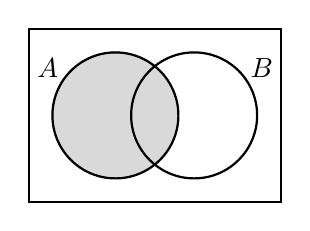
\begin{tikzpicture}[scale=0.4]
		\def\universal{(-4,-2.75) -- (4,-2.75) -- (4,2.75) -- (-4,2.75) -- cycle}		
		\def\firstcircle{(-1.25,0) circle (2cm)}
		\def\secondcircle{(1.25,0) circle (2cm)}
		\draw[fill=gray!30] \firstcircle;
		\draw[thick] \firstcircle;
		\draw[thick] \secondcircle;
		\draw[thick] \universal;
		\node at (-3.4,1.5) {$A$};
		\node at (3.4,1.5) {$B$};
	\end{tikzpicture}\\
	$A$
	\end{center}
  \end{minipage}
  \hspace{1.0cm}
   \begin{minipage}[th!]{0.2\textwidth}
  	\begin{center}
  	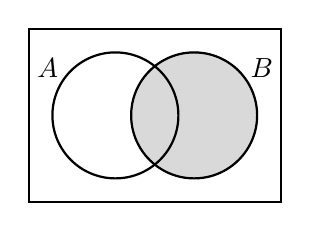
\begin{tikzpicture}[scale=0.4]
		\def\universal{(-4,-2.75) -- (4,-2.75) -- (4,2.75) -- (-4,2.75) -- cycle}		
		\def\firstcircle{(-1.25,0) circle (2cm)}
		\def\secondcircle{(1.25,0) circle (2cm)}
		\draw[fill=gray!30] \secondcircle;
		\draw[thick] \firstcircle;
		\draw[thick] \secondcircle;
		\draw[thick] \universal;
		\node at (-3.4,1.5) {$A$};
		\node at (3.4,1.5) {$B$};
	\end{tikzpicture}\\
	$B$
	\end{center}
  \end{minipage}
    \hspace{1.0cm}
   \begin{minipage}[th!]{0.2\textwidth}
  	\begin{center}
  	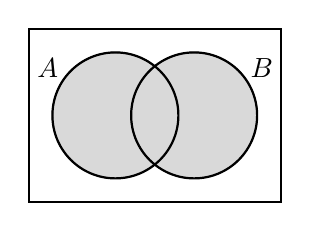
\begin{tikzpicture}[scale=0.4]
		\def\universal{(-4,-2.75) -- (4,-2.75) -- (4,2.75) -- (-4,2.75) -- cycle}		
		\def\firstcircle{(-1.25,0) circle (2cm)}
		\def\secondcircle{(1.25,0) circle (2cm)}
		\draw[fill=gray!30] \firstcircle;
		\draw[fill=gray!30] \secondcircle;
		\draw[thick] \firstcircle;
		\draw[thick] \secondcircle;
		\draw[thick] \universal;
		\node at (-3.4,1.5) {$A$};
		\node at (3.4,1.5) {$B$};
	\end{tikzpicture}\\
	$A \cup B$
	\end{center}
  \end{minipage}

\vspace{0.5cm}

   \begin{minipage}[th!]{0.2\textwidth}
  	\begin{center}
  	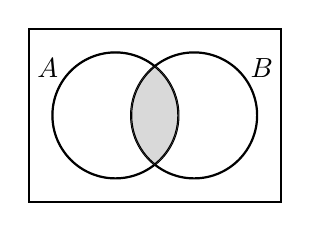
\begin{tikzpicture}[scale=0.4]
		\def\universal{(-4,-2.75) -- (4,-2.75) -- (4,2.75) -- (-4,2.75) -- cycle}		
		\def\firstcircle{(-1.25,0) circle (2cm)}
		\def\secondcircle{(1.25,0) circle (2cm)}
		\draw[thick] \firstcircle;
		\draw[thick] \secondcircle;
		\draw[thick] \universal;
		\node at (-3.4,1.5) {$A$};
		\node at (3.4,1.5) {$B$};
		\draw[clip] \firstcircle;
		\draw[clip] \secondcircle;
		\fill[gray!30] (0,0) circle (2cm);
		\draw[thick] \firstcircle;
		\draw[thick] \secondcircle;
	\end{tikzpicture}\\
	$A \cap B$
	\end{center}
  \end{minipage}
\hspace{1.0cm}  
 \begin{minipage}[th!]{0.2\textwidth}
  	\begin{center}
  	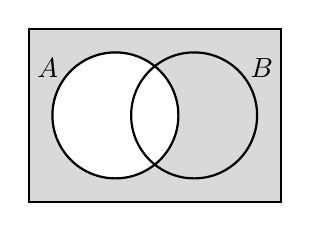
\begin{tikzpicture}[scale=0.4]
		\def\universal{(-4,-2.75) -- (4,-2.75) -- (4,2.75) -- (-4,2.75) -- cycle}		
		\def\firstcircle{(-1.25,0) circle (2cm)}
		\def\secondcircle{(1.25,0) circle (2cm)}
		\draw[fill=gray!30] \universal;
		\draw[fill=white] \firstcircle;
		\draw[thick] \firstcircle;
		\draw[thick] \secondcircle;
		\draw[thick] \universal;
		\node at (-3.4,1.5) {$A$};
		\node at (3.4,1.5) {$B$};
	\end{tikzpicture}\\
	$A^c$
	\end{center}
  \end{minipage}
  \hspace{1.0cm}
 \begin{minipage}[th!]{0.2\textwidth}
  	\begin{center}
  	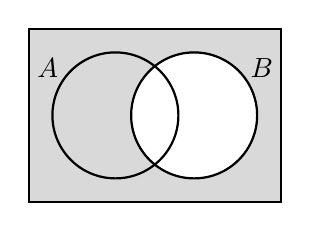
\begin{tikzpicture}[scale=0.4]
		\def\universal{(-4,-2.75) -- (4,-2.75) -- (4,2.75) -- (-4,2.75) -- cycle}		
		\def\firstcircle{(-1.25,0) circle (2cm)}
		\def\secondcircle{(1.25,0) circle (2cm)}
		\draw[fill=gray!30] \universal;
		\draw[fill=white] \secondcircle;
		\draw[thick] \firstcircle;
		\draw[thick] \secondcircle;
		\draw[thick] \universal;
		\node at (-3.4,1.5) {$A$};
		\node at (3.4,1.5) {$B$};
	\end{tikzpicture}\\
	$B^c$
	\end{center}
  \end{minipage}
\caption{Vennn diagrams}
\label{F:Venn}
\end{center}
\end{figure}
 
As we have discussed, to prove that two sets $X$ and $Y$ are equal we prove that each is a subset of the other. The next example provides another illustration of the  idea.

\begin{example} \label{ex:set_eq} Let $A$, $B$, and $C$ be sets. We will prove that $A \cap (B \setminus C) = (A \cap B) \setminus (A \cap C)$. 

To prove this set equality we must prove that $A \cap (B \setminus C) \subseteq (A \cap B) \setminus (A \cap C)$ and $(A \cap B) \setminus (A \cap C) \subseteq A \cap (B \setminus C)$. We start with $A \cap (B \setminus C) \subseteq (A \cap B) \setminus (A \cap C)$.

To prove that $A \cap (B \setminus C) \subseteq (A \cap B) \setminus (A \cap C)$, we need to demonstrate that every element in $A \cap (B \setminus C)$ is also in $(A \cap B) \setminus (A \cap C)$. To do this, we select an arbitrary element in $A \cap (B \setminus C)$ and show that this element is in $(A \cap B) \setminus (A \cap C)$. Let $x \in A \cap (B \setminus C)$. Then $x \in A$ and $x \in B \setminus C$. The fact that $x \in B \setminus C$ implies that $x \in B$ but $x \notin C$. Therefore, $x \in A$ and $x \in B$, but $x \notin C$. This implies that $x \in A$ and $x \in B$, but $x \in A$ and $x \notin C$. So $x \in A$ and $x \in B$, but $x \notin A \cap C$. We conclude that $x \in (A \cap B) \setminus (A \cap C)$. This proves that $A \cap (B \setminus C) \subseteq (A \cap B) \setminus (A \cap C)$.

For the reverse containment, we let $y \in (A \cap B) \setminus (A \cap C)$. So $y \in A \cap B$ but $y \notin A \cap C$. Since $y \in A \cap B$, we know that $y \in A$ and $y \in B$. The fact that $y \notin A \cap C$ means that $y \notin C$. So $y \in A$, $y \in B$, and $y \notin C$.  Thus, $y \in A$ and $y \in B \setminus C$. We conclude that $y \in A \cap (B \setminus C)$, which shows that $(A \cap B) \setminus (A \cap C) \subseteq A \cap (B \setminus C)$. The two containments, $A \cap (B \setminus C) \subseteq (A \cap B) \setminus (A \cap C)$ and $(A \cap B) \setminus (A \cap C) \subseteq A \cap (B \setminus C)$ demonstrate that $A \cap (B \setminus C) = (A \cap B) \setminus (A \cap C)$.

\end{example}

We will use the ideas in Activity \ref{act:set_equality} and Example \ref{ex:set_eq} to prove set equalities throughout this text. The next activity will provide some additional practice. 
 
\begin{activity} \label{act:sets_1} In this activity we work with unions, intersections, and complements of sets. Let $A$ and $B$ be sets. 
	\ba
	\item  Let $A = \{1,2,3,4,5,6\}$ and $B = \{2,4,6,8,10\}$, with $U = \{1,2,3,4,5,6,7,8,9,10\}$. 
		\begin{enumerate}[i.]
		\item Determine the elements in $A \cup B$ and $A \cap B$. What are the elements in $(A \cup B)^c$ and $(A \cap B)^c$?
		
		\item Determine the elements in $A^{c} \cup B^{c}$ and $A^{c} \cap B^{c}$. 

		\end{enumerate}

%	If $U = \{a,b,c,d,e,f,g\}$ and $A = \{c,e,g\}$, what is $U \setminus A$? 
	
	\item Let $A$ and $B$ be arbitrary subsets of a universal set $U$. There are connections between $A$, $B$ and their complements, unions, and intersections. 
		\begin{enumerate}[i.]
		\item Use Venn diagrams to draw $(A \cup B)^c$ and $(A \cap B)^c$.  
		
		\item Use the Venn diagrams and the result of (a) to find and prove a relationship between $A^c$, $B^c$ and $(A \cup B)^c$.

		\item Use the Venn diagrams and the result of (a) to find and prove a relationship between $A^c$, $B^c$ and $(A \cap B)^c$.

		\end{enumerate}
		
	\ea
\end{activity}

\begin{comment}

\ActivitySolution

\ba
\item Let $A = \{1,2,3,4,5,6\}$ and $B = \{2,4,6,8,10\}$, with $U = \{1,2,3,4,5,6,7,8,9,10\}$. 
	\begin{enumerate}[i.]
	
	\item In this example we have 
\[A \cup B = \{1,2,3,4,5,6,8,10\} \ \text{ and } \ A \cap B = \{2,4,6\}.\]

	\item Given $A \cap B$ and $A \cup B$ from part i.,  
\[(A \cap B)^c = \{1,3,5,7,8,9,10\} \ \text{ and } \ A^{c} \cup B^{c} = \{1,3,5,7,8,9,10\}\]
and
\[(A \cup B)^c = \{7,9\} \ \text{ and } \ A^{c} \cap B^{c} = \{7,9\}.\]

	\end{enumerate}
	
%\item In this example we have $U \setminus A = \{a,b,d,f\}$.

\item Venn diagrams illustrating the sets $(A \cup B)^c$ and $(A \cap B)^c$ are shown below.
\begin{center}
 \begin{minipage}[th!]{0.2\textwidth}
  	\begin{center}
  	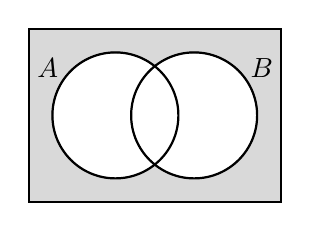
\begin{tikzpicture}[scale=0.4]
		\def\universal{(-4,-2.75) -- (4,-2.75) -- (4,2.75) -- (-4,2.75) -- cycle}		
		\def\firstcircle{(-1.25,0) circle (2cm)}
		\def\secondcircle{(1.25,0) circle (2cm)}
		\draw[fill=gray!30] \universal;
		\draw[fill=white] \firstcircle;
		\draw[fill=white] \secondcircle;
		\draw[thick] \firstcircle;
		\draw[thick] \secondcircle;
		\draw[thick] \universal;
		\node at (-3.4,1.5) {$A$};
		\node at (3.4,1.5) {$B$};
	\end{tikzpicture}\\
	$(A \cup B)^c$
	\end{center}
  \end{minipage}
  \hspace{1.0cm}
 \begin{minipage}[th!]{0.2\textwidth}
  	\begin{center}
  	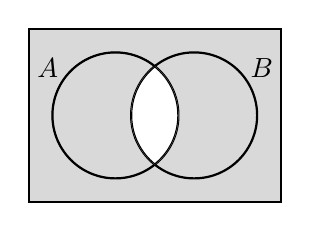
\begin{tikzpicture}[scale=0.4]
		\def\universal{(-4,-2.75) -- (4,-2.75) -- (4,2.75) -- (-4,2.75) -- cycle}		
		\def\firstcircle{(-1.25,0) circle (2cm)}
		\def\secondcircle{(1.25,0) circle (2cm)}
		\draw[fill=gray!30] \universal;	
		\draw[thick] \firstcircle;
		\draw[thick] \secondcircle;
		\draw[thick] \universal;
		\node at (-3.4,1.5) {$A$};
		\node at (3.4,1.5) {$B$};
		\draw[clip] \firstcircle;
		\draw[clip] \secondcircle;
		\fill[white] (0,0) circle (2cm);
		\draw[thick] \firstcircle;
		\draw[thick] \secondcircle;
	\end{tikzpicture}\\
	$(A \cap B)^c$
	\end{center}
  \end{minipage}
\end{center}

	\begin{enumerate}[i.]
	\item The Venn diagrams and (a) indicate that $(A \cup B)^c = A^c \cap B^c$. To prove this statement, start by letting $x \in (A \cup B)^c$. Then $x \notin (A \cup B)$. So $x \notin A$ and $x \notin B$. This means that $x \in A^c$ and $x \in B^c$, which implies that $x \in (A^c \cap B^c)$. We conclude that $(A \cup B)^c \subseteq (A^c \cap B^c)$.
	
Now suppose that $x \in (A^c \cap B^c)$. Then $x \in A^c$ and $x \in B^c$. So $x \notin A$ and $x \notin B$ and $x \notin (A \cup B)$. From this it follows that $x \in (A \cup B)^c$. We conclude that $(A^c \cap B^c) \subseteq (A \cup B)^c$.The two containments demonstrate that $(A \cup B)^c = A^c \cap B^c$.

	\item The Venn diagrams and (a) indicate that $(A \cap B)^c = A^c \cup B^c$.  prove this statement, start by letting $x \in (A \cap B)^c$. Then $x \notin (A \cap B)$. So $x \notin A$ or $x \notin B$. This means that $x \in A^c$ or $x \in B^c$, which implies that $x \in (A^c \cup B^c)$. We conclude that $(A \cap B)^c \subseteq (A^c \cup B^c)$.
	
Now suppose that $x \in (A^c \cup B^c)$. Then $x \in A^c$ or $x \in B^c$. So $x \notin A$ or $x \notin B$, which means $x \notin (A \cap B)$. But this implies that $x \in (A \cap B)^c$. We conclude that $(A^c \cup B^c) \subseteq (A \cap B)^c$.The two containments demonstrate that $(A \cap B)^c = A^c \cup B^c$.

	\end{enumerate}
	
\ea	

\end{comment}

In Activity \ref{act:sets_1} we worked with the union and intersection of two sets. There is no reason to restrict these definitions to only two sets, as the next activity illustrates. 

\begin{activity}  To define an infinite collection of sets we often use what is called an \emph{indexing set}. An indexing set allows us to consider a collection of objects that are in one-to-one correspondence with a set like the positive integers, or even the real numbers. When using an indexing set, we generally make a statement such as ``let $\{A_{\alpha}\}$ for $\alpha \in I$ be a collection of sets indexed by some set $I$". The collection $\{A_{\alpha}\}_{\alpha \in I}$ is called an \emph{indexed family of sets}.\index{indexed family of sets} 

	\ba
	\item The set $I$ could be finite. As an example, let $A_{n} = \{1, 2, 3, \ldots n\}$ for $n$ in the set $I = \{1,2,3, \ldots, 10\}$.
		\begin{enumerate}[i.]
		\item What is $A_5$? What is $A_{8}$? 
		
		\item How many sets are in the indexed family $\{A_n\}_{n \in I}$?
		\end{enumerate}
	
	\item The indexing set can be infinite. For example, let $A_{\alpha} = [0, |\alpha|)$ for $\alpha$ in the set $\R$ (where $[a,b)$ is the interval consisting of the real numbers $x$ such that $a \leq x < b$). In this case, what is $A_5$? What is $A_{\pi}$?  What is $A_{-\frac{2}{3}}$? 
		
	\item We have defined the union and intersection of two sets. The same idea can be extended to define the union and intersection of an indexed collection of sets. 
		\begin{enumerate}[i.]
		\item Recall that if $A$ and $B$ are sets, the intersection $A \cap B$ is the set $\{x \mid x \in A \text{ and } x \in B\}$. How can we extend this definition from two sets to any collection of sets? In other words, how do we \textbf{define} \index{set!arbitrary intersection} 
	\[\bigcap_{\alpha \in I} A_{\alpha}?\]
In the example in (b), what set is $\ds \bigcap_{\alpha \in \R} A_{\alpha}$?
		
	\item Recall that if $A$ and $B$ are sets, the union $A \cup B$ is the set $\{x \mid x \in A \text{ or } x \in B\}$. How can we extend this definition from two sets to any collection of sets? In other words, how do we \textbf{define} \index{set!arbitrary union} 
	\[\bigcup_{\alpha \in I} A_{\alpha}?\]
In the example in (b), what set is $\ds \bigcup_{\alpha \in \R} A_{\alpha}$?
	
	\end{enumerate}
	
	\ea

\end{activity}

\begin{comment}

\ActivitySolution

	\ba
	\item 
		\begin{enumerate}[i.]
		\item In this case we have $A_5 = \{1,2,3,4,5\}$ and $A_{8} = \{1,2,3,4,5,6,7,8\}$. 
		
		\item Since the indexing set has 10 elements there are 10 sets in the indexed collection of sets.
		
		\end{enumerate}
		
	\item In this case we have $A_5 = [0,5)$, $A_{\pi} = [0,\pi)$, and $A_{-\frac{2}{3}} = \left[0, \frac{2}{3}\right)$. 
	
	\begin{enumerate}[i.]

		
	\item We define $\bigcap_{\alpha \in I} A_{\alpha}$ as follows:
	\[\bigcap_{\alpha \in I} A_{\alpha} = \{x \mid x \in A_{\alpha} \text{ for all } \alpha \in I\}.\]
In our example from (b) we claim that $\bigcap_{\alpha \in I} A_{\alpha} = \{0\}$. To prove this statement, we have that $0 \in A_{\alpha}$ for every $\alpha \in \R$ by definition. So $\{0\} \subseteq  \bigcap_{\alpha \in I} A_{\alpha} = \{0\}$. Now we show that $0$ is the only element in $\bigcap_{\alpha \in I} A_{\alpha} = \{0\}$. Let $x$ be a nonzero real number. Then $A_{x/2} = [0, |x|/2)$ does not contain $x$. So $x \notin \bigcap_{\alpha \in I} A_{\alpha} = \{0\}$. We conclude that $\bigcap_{\alpha \in I} A_{\alpha} = \{0\}$.

	
		\item We define $\bigcup_{\alpha \in I} A_{\alpha}$ as follows:
	\[\bigcup_{\alpha \in I} A_{\alpha} = \{x \mid x \in A_{\alpha} \text{ for some } \alpha \in I\}.\]
In our example from (b) we claim that $\bigcup_{\alpha \in I} A_{\alpha} = [0, \infty)$. Since $A_{\alpha} \subset [0, \infty)$ for every $\alpha \in \R$, it follows that $\bigcup_{\alpha \in I} A_{\alpha} \subseteq [0, \infty)$. Now we prove the reverse containment. Let $x \in [0, \infty)$. Then $x \in [0, 2x) = A_{2x}$. Then $x \in \bigcup_{\alpha \in I} A_{\alpha}$ and $[0, \infty) \subseteq \bigcup_{\alpha \in I} A_{\alpha}$. The two containments demonstrate that  $\bigcup_{\alpha \in I} A_{\alpha} = [0, \infty)$.


	\end{enumerate}
	
\ea

\end{comment}

These properties $(A \cap B)^c = A^c \cup B^c$ and $(A \cup B)^c = A^c \cap B^c$ that we learned about in Activity \ref{act:sets_1} are called DeMorgan's Laws. These laws apply to any union or intersection of sets, finite or infinite. The proofs are left Exercise (\ref{ex:DeMorgan}).   

\begin{theorem}[DeMorgan's Laws] Let $\{A_{\alpha}\}$ is a collection of sets indexed by a set $I$ in some universal set $U$. Then 
\begin{enumerate}
\item $\displaystyle \left(\bigcup_{\alpha \in I} A_{\alpha}\right)^c = \bigcap_{\alpha \in I} A_{\alpha}^c$ 
\item $\displaystyle \left(\bigcap_{\alpha \in I} A_{\alpha}\right)^c = \bigcup_{\alpha \in I} A_{\alpha}^c$ 
\end{enumerate}
\end{theorem}

\begin{activity} ~
\ba
\item Verify DeMorgan's Laws in the specific case of $A_{\alpha} = \{1, 2, 3, \ldots \alpha\}$ in $U = \Z$, where $\alpha$ is any element of the indexing set $I = \Z^+$. 

\item Why should the complement of a union be an intersection and why should the complement of an intersection be a union? (Hint: Consider the definitions of unions and intersections.)

\ea

\end{activity}

\begin{comment}

\ActivitySolution 

\ba

\item Let $\Z^- = \{n \in \Z \mid n < 0\}$. First note that $A_{\alpha}^c = \Z^- \cup \{0\} \cup \{\alpha+1, \alpha+2, \ldots\}$. So $\bigcap_{\alpha \in I} A_{\alpha}^c =  \Z^- \cup \{0\}$. Also, $\bigcup_{\alpha \in I} A_{\alpha} = \Z^+$, so $\left(\bigcup_{\alpha \in I} A_{\alpha}\right)^c = \Z^- \cup \{0\}$. 

Since $A_1^c = \Z \setminus \{1\}$, and $1$ is not an element of any $A_{\alpha}^c$, we have $\bigcup_{\alpha \in I} A_{\alpha}^c = \Z \setminus \{1\}$. Since $A_1 = \{1\}$, the only element common to all of the $A_{\alpha}$ is $1$, and $\bigcap_{\alpha \in I} A_{\alpha} = \{1\}$. So $\left(\bigcap_{\alpha \in I} A_{\alpha}\right)^c = \Z \setminus \{1\}$. 

\item Recall that a union is defined as an ``or" statement and an intersection is an ``and" statement. That is $A \cup B$ is the set of elements in $A$ or $B$, and $A \cap B$ is the set of elements in $A$ and $B$.  A complement is a negation, and the negation of ``$A$ or $B$" is ``(not $A$) and (not $B$)". Similarly, the negation of ``$A$ and $B$" is ``(not $A$) or (not $B$)".   

\ea

\end{comment}


\csection{Cartesian Products of Sets}

The final operation on sets that we discuss is the \emph{Cartesian product} (or \emph{cross product}). This is an operation that we have seen before. When we draw the graph of a line $y = mx+b$ in the plane, we plot the points $(x,mx+b)$. These points are ordered pairs of real numbers. We can extend this idea to any sets. 

\begin{definition} Let $A$ and $B$ are sets. The \textbf{Cartesian product}\index{Cartesian product} of $A$ and $B$ is the set 
\[A \times B = \{(a,b) \mid a \in A \text{ and } b \in B\}.\]
\end{definition}

In other words, the Cartesian product of $A$ and $B$ is the set of ordered pairs $(a,b)$ with $a$ coming from $A$ and $b$ coming from $B$. Note that the order is important. 

\begin{activity} ~
	\ba
	\item List all of the elements in $\{\text{red}, \text{blue}\} \times \{\text{car}, \text{truck}, \text{van}\}$. 
	
	\item If $A$ has $m$ elements and $B$ has $n$ elements, how many elements does the set $A \times B$ have? Explain.

	\ea
	
\end{activity}

\begin{comment}

\ActivitySolution

	\ba
	\item The elements are 
	\begin{center} (red,car), (red,truck), (red,van), (blue,car), (blue,truck), (blue,van).\end{center}
	
	\item Any element in $A \times B$ pairs an element of $A$ with an element of $B$. We can choose $n$ elements from $A$ and $m$ from $B$, so the total number of pairings is $nm$. 

	\ea
	

\end{comment}

There is no reason to restrict ourselves to a Cartesian product of just two sets. This is an idea that we have encountered before. The Cartesian product $\R \times \R$ is the standard real plane that we denote as $\R^2$ and the Cartesian product $\R \times \R \times \R$ is the three-dimensional real space denoted as $\R^3$. If we have an indexed collection $\{X_{i}\}$ of sets, with $i$ running through the set of positive integers, then we can define the Cartesian product of the sets $X_{i}$ as the set of infinite sequences $(x_1, x_2, \ldots, x_n, \ldots)$, where $x_i \in X_i$ for each $i \in \Z^+$. We denote this cartesian product as 
\[\Pi_{i \in \Z^+} X_i = \Pi_{i=1}^{\infty} X_i. \]
The capital pi ($\Pi$) is used to represent a product an an analog of the capital sigma ($\Sigma$) that is used to represent a sum. We will study sequences in more detail later. 


To conclude this section we summarize some properties of sets. Many of these properties can be extended to arbitrary collections of sets. Most of the proofs are straightforward. The associative and distributive laws are left for Exercise (\ref{ex:set_props}). 

\newpage
\begin{theorem} Let $A$, $B$, and $C$ be subsets of a universal set $U$. 
\begin{multicols}{2}
\begin{description}
\item[Properties of the Empty Set.]  ~
	\begin{enumerate}[i.]
	\item $A \cap \emptyset = \emptyset$ 
	\item $A \cup \emptyset = A$ 
	\item $A-\emptyset = A$ 
	\item $\emptyset^c = U$
	\end{enumerate}
\item[Properties of the Universal Set.] ~
	\begin{enumerate}[i.]
	\item $A \cap U = A$ 
	\item $A \cup U = U$ 
	\item $A-U = \emptyset$ 
	\item $U^c = \emptyset$  
	\end{enumerate}
\item[Idempotent Laws.] ~
	\begin{enumerate}[i.]
	\item  $A \cap A = A$ 
	\item $A \cup A = A$ 
	\end{enumerate} 
	\vspace{24pt}
\item[Commutative Laws.] ~
	\begin{enumerate}[i.]
	\item $A \cap B  = B \cap A$
	\item $A \cup B = B \cup A$  
	\end{enumerate}
\item[Associative Laws.] ~
	\begin{enumerate}[i.]
	\item $(A \cap B) \cap C = A \cap (B \cap C)$ 
	\item $(A \cup B) \cup C = A \cup (B \cup C)$ 
	\end{enumerate}
\item[Distributive Laws.] ~
	\begin{enumerate}[i.]
	\item $A \cap (B \cup C) = (A \cap B) \cup (A \cap C)$ 
	\item$A \cup (B \cap C) = (A \cup B) \cap (A \cup C)$ 
	\end{enumerate}
\item[Basic Properties.] ~
	\begin{enumerate}[i.]
	\item $\left(A^c\right)^c = A$ 
	\item $A - B = A \cap B^c$ 
	\end{enumerate}
\item[Subsets and Complements.] ~

$A \subseteq B$ \text{ if and only if } $B^c \subseteq A^c$
\end{description}
\end{multicols}
\end{theorem}

\csection{Summary}
Important ideas that we discussed in this section include the following.
\begin{itemize}
\item We can consider a set to be a well-defined collection of elements.
\item A subset of a set is any collection of elements from that set. That is, a subset $S$ of a set $X$ is a set with the property that if $s \in S$, then $s \in X$. 
\item If $X$ and $Y$ are sets, then the union $X \cup Y$ is the set 
\[X \cup Y = \{z \mid z \in X \text{ or } z \in Y\}.\]
The union of an arbitrary collection $\{X_{\alpha}\}$ of sets for $\alpha$ in some indexing set $I$ is the set 
\[\bigcup_{\alpha \in I} X_{\alpha} = \{z \mid z \in X_{\beta} \text{ for some } \beta \in I\}.\]
\item If $X$ and $Y$ are sets, then the intersection $X \cap Y$ is the set 
\[X \cap Y = \{z \mid z \in X \text{ and } z \in Y\}.\]
The intersection of an arbitrary collection $\{X_{\alpha}\}$ of sets for $\alpha$ in some indexing set $I$ is the set 
\[\bigcap_{\alpha \in I} X_{\alpha} = \{z \mid z \in X_{\beta} \text{ for all } \beta \in I\}.\]
\item If $X$ is a set and $A$ is a subset of $X$, then the complement of $A$ in $X$ is the set 
\[A^c = \{x \in X \mid x \notin A\}.\]
\item If $\{X_{i}\}$ is a collection of sets with $i$ in some indexing set $I$, where $I$ is finite or $I$ is the set of positive integers, the Cartesian product $\Pi_{i \in I} X_i$ of the sets $X_{i}$ as the set of all ordered tuples of the form $(x_i)$ where $i \in I$. 
\end{itemize}

\csection{Exercises}

\be

\item Let $A$, $B$, and $C$ be subsets of a set $X$. Express each of the following sets in mathematical notation using the symbols $\cup$, $\cap$, and $\setminus$.
\ba
\item The elements of $X$ that belong to $A$ and $B$, but not $C$.

\item The elements of $X$ that belong to $C$ and either $A$ or $B$.

\item The elements of $X$ that belong to $A$ but not to both $B$ and $C$.

\item The elements of $X$ that belong to none of the sets $A$, $B$, and $C$.

\item The elements of $X$ that fail to belong to at least two of the sets $A$, $B$, and $C$.

\item  The elements of $X$ that fail to belong to at most one of the sets $A$, $B$, and $C$.

\ea

\begin{comment}

\ExerciseSolution

\ba
\item This set $A \cap B$ is the set of elements that belong to both $A$ and $B$. So the set in question is $(A \cap B) \setminus C$. 

\item The set $A \cup B$ is the set of elements belonging to $A$ or $B$. So the set in question is $C \cap (A \cup B)$. 

\item The set of elements that belong to both $B$ and $C$ is $B \cap C$. So the set in question is $A \setminus (B \cap C)$. 

\item We remove the elements of $A \cup B \cup C$ from $X$. So the set in question is $X \setminus (A \cup B \cup C)$. 

\item The set of elements that belong to at least two of the sets $A$, $B$, and $C$ is $(A \cap B) \cup (A \cap C) \cup (B \cap C)$. So the set in question is $X \setminus ((A \cap B) \cup (A \cap C) \cup (B \cap C))$. 

\item  The set of elements that belong to $A$ but not $B$ or $C$ is $A \setminus (B \cup C)$. So the set of elements that belong to exactly one of $A$, $B$, or $C$ is $(A \setminus (B \cup C)) \cup (B \setminus (A \cup C)) \cup (C \setminus (A \cup B))$. The set of elements that belong to none of $A$, $B$, or $C$ is $X \setminus(A \cup B \cup C)$. So the set in question is 
\[(A \setminus (B \cup C)) \cup (B \setminus (A \cup C)) \cup (C \setminus (A \cup B)) \cup (X \setminus(A \cup B \cup C)).\]

\ea

\end{comment}



\item Let $X \subset Y \subset Z$. Prove or disprove.
\ba
\item $C_Y(X) \subset C_Z(X)$.

\item $Z \setminus (Y \setminus X) = X \cup (Z \setminus Y)$. 


\ea

\begin{comment}

\ExerciseSolution

\ba
\item  To prove this containment, we choose an arbitrary element from $C_Y(X)$ and show that the element is also in $C_Z(X)$. Suppose $t \in C_Y(X)$. Then $t \in Y$ but $t \not\in X$. Since $Y \subset Z$, it follows that $t \in Z$. So $t \in Z$ but $t \notin X$. This means $t \in C_Z(X)$. We conclude that $C_Y(X) \subset C_Z(X)$.

\item  To prove $Z \setminus (Y \setminus X) \subseteq X \cup (Z \setminus Y)$, suppose that $t \in Z \setminus (Y \setminus X)$. By definition, $t \in Z$ but $t \notin (Y\setminus X)$. So $t \in X$ or $t \notin Y$. This gives us two possibilities: $t \in Z$ and $t \in X$ or $t \in Z$ and $t \notin Y$. 
\begin{itemize}
\item If $t \in X$ and $t \in Z$, then $X \subset Z$ implies $t \in X$. 
\item If $t \in Z$ and $t \notin Y$, then $t \in Z\setminus Y$. 
\end{itemize}
Thus, we either have $t \in X$ or $t \in Z\setminus Y$. This is the same as saying $t \in X \cup (Z\setminus Y)$. So  $Z \setminus (Y\setminus X) \subseteq X \cup (Z\setminus Y)$.

For the reverse containment, suppose $t \in X \cup (Z\setminus Y)$. Then $t \in X$ or $t \in Z\setminus Y$. We consider the cases.  
\begin{itemize}
\item Suppose $t \in X$. Then $X \subseteq Z$ implies $t \in Z$. The fact that $t \in X$ means that $t \notin Y\setminus X$. Thus, $t \in Z \setminus (Y\setminus X)$.
\item Now suppose that $t \in Z\setminus Y$. Since $Z\setminus Y \subseteq Z$, it follows that $t \in Z$. The facts that $Y\setminus X \subseteq Y$ and $t \notin Y$ also show that $t \notin Y\setminus X$. Thus, $t \in Z \setminus (Y\setminus X)$. 
\end{itemize}
In either case we have $t \in Z \setminus (Y\setminus X)$, and so $X \cup (Z\setminus Y) \subseteq Z \setminus (Y\setminus X)$. The two containments combine to verify that $Z \setminus (Y\setminus X) = X \cup (Z\setminus Y)$.

\ea

\end{comment}

\item \label{ex:set_props} Let $A$ and $B$ be subsets of a universal set $U$. Prove the associative and distributive laws. That is, prove each of the following.
	\ba
	\item $(A \cap B) \cap C = A \cap (B \cap C)$ 
	\item $(A \cup B) \cup C = A \cup (B \cup C)$ 
	\item $A \cap (B \cup C) = (A \cap B) \cup (A \cap C)$ 
	\item$A \cup (B \cap C) = (A \cup B) \cap (A \cup C)$ 
	\ea
	
\begin{comment}

\ExerciseSolution

	\ba
	\item Suppose that $x \in (A \cap B) \cap C$. Then $x \in A \cap B$ and $x \in C$. So $x \in A$ and $x \in B$, and $x \in C$. It follows that $x \in A$ and $x \in B \cap C$, so $x \in  A \cap (B \cap C)$. Thus, $(A \cap B) \cap C \subseteq  A \cap (B \cap C)$. 
	
	Now suppose that $x \in A \cap (B \cap C)$. Then $x \in A$ and $x \in B \cap C$. So $x \in A$, and $x \in B$ and $x \in C$. Thus, $x \in A \cap B$ and $x \in C$ or $x \in (A \cap B) \cap C$. It follows that $A \cap (B \cap C) \subseteq (A \cap B) \cap C$. The two containments show that $(A \cap B) \cap C = A \cap (B \cap C)$.
	
	\item Suppose that $x \in (A \cup B) \cup C$. Then $x \in A \cup B$ or $x \in C$. Thus, $x \in A$ or $x \in B$, or $x \in C$. This means that $x \in A$ or $x \in B \cup C$. It follows that $x \in A \cup (B \cup C)$ and so $(A \cup B) \cup C \subseteq A \cup (B \cup C)$. 
	
	Now suppose that $x \in A \cup (B \cup C)$. Then $x \in A$ or $x \in B \cup C$. From this we can say that $x \in A$, or $x \in B$ or $x \in C$. Then $x \in A \cup B$ or $x \in C$. It follows that that $x \in (A \cup B) \cup C$ and $A \cup (B \cup C) \subseteq (A \cup B) \cup C$. The two containments show that $(A \cup B) \cup C = A \cup (B \cup C)$. 
	
	\item Suppose that $x \in A \cap (B \cup C)$. Then $x \in A$ and $x \in B \cup C$. So $x \in A$ and $x$ is in one of $B$ or $C$. If $x in B$, then $x \in A \cap B$. If $x \in C$, then $x \in A \cap C$. In either case, $x \in (A \cap B) \cup (A \cap C)$. So $A \cap (B \cup C) \subseteq (A \cap B) \cup (A \cap C)$.
	
	Now suppose that $x \in (A \cap B) \cup (A \cap C)$. Then $x \in A \cap B$ or $x \in A \cap C$. If $x \in A \cap B$, then $a \in A$ and $x \in B \subseteq B \cup C$ and so $x \in A \cap (B \cup C)$. Similarly, if $x \in A \cap C$, then $a \in A$ and $x \in C \subseteq B \cup C$ and so $x \in A \cap (B \cup C)$. Thus, $(A \cap B) \cup (A \cap C) \subseteq A \cap (B \cup C)$. The two containments show that $A \cap (B \cup C) = (A \cap B) \cup (A \cap C)$.
	
	\item Suppose that $x \in A \cup (B \cap C)$. Then $x \in A$ or $x \in B \cap C$. If $x \in A$, then $x \in A \cup B$ and $x \in A \cup C$ and $x \in (A \cup B) \cap (A \cup C)$. If $x \in B \cap C$,  then $x \in B \subseteq A \cup B$ and $x \in C \subseteq A \cup C$. So $x \in (A \cup B) \cap (A \cup C)$. We conclude that $A \cup (B \cap C) \subseteq (A \cup B) \cap (A \cup C)$.
	
	Now suppose that $x \in (A \cup B) \cap (A \cup C)$. Then $x \in A \cup B$ and $x \in A \cup C$. If $x \in A$, then $x \in A \cup (B \cap C)$. If $x \notin A$, then $x \in B$ and $x \in C$. So $x \in B \cap C \subseteq A \cup (B \cap C)$. It follows that $(A \cup B) \cap (A \cup C) \subseteq A \cup (B \cap C)$. The two containments show that $A \cup (B \cap C) = (A \cup B) \cap (A \cup C)$.
	
	\ea
	

\end{comment}

\item \label{ex:DeMorgan} Prove DeMorgan's Laws. That is, let $\{A_{\alpha}\}$ be a collection of sets indexed by a set $I$ in some universal set $U$. Prove that 
\begin{enumerate}
\item $\displaystyle \left(\bigcup_{\alpha \in I} A_{\alpha}\right)^c = \bigcap_{\alpha \in I} A_{\alpha}^c$ 
\item $\displaystyle \left(\bigcap_{\alpha \in I} A_{\alpha}\right)^c = \bigcup_{\alpha \in I} A_{\alpha}^c$ 
\end{enumerate}

\begin{comment}

\ExerciseSolution  Let $\{A_{\alpha}\}$ be a collection of sets indexed by a set $I$ in some universal set $U$. First we show that $\displaystyle \left(\bigcup_{\alpha \in I} A_{\alpha}\right)^c = \bigcap_{\alpha \in I} A_{\alpha}^c$. Let $x \in \displaystyle \left(\bigcup_{\alpha \in I} A_{\alpha}\right)^c$. Then $x \in U$ but $x$ cannot be in any of the $A_{\alpha}$. So $x \in A_{\alpha}^c$ for every $\alpha \in I$ and $x \in \displaystyle \bigcap_{\alpha \in I} A_{\alpha}^c$. Thus, $\displaystyle \left(\bigcup_{\alpha \in I} A_{\alpha}\right)^c \subseteq \bigcap_{\alpha \in I} A_{\alpha}^c$. For the reverse containment, suppose $x \in \bigcap_{\alpha \in I} A_{\alpha}^c$. Then $x \in A_{\alpha}^c$ for every $\alpha \in I$. This means that $x \notin A_{\alpha}$ for every $\alpha \in I$. That is, $x \notin \displaystyle \bigcup_{\alpha \in I} A_{\alpha}$. Thus $x \in \displaystyle \left(\bigcup_{\alpha \in I} A_{\alpha}\right)^c$. This shows that $\displaystyle  \bigcap_{\alpha \in I} A_{\alpha}^c \subseteq \left(\bigcup_{\alpha \in I} A_{\alpha}\right)^c$. The two containments demonstrate that $\displaystyle  \bigcap_{\alpha \in I} A_{\alpha}^c = \left(\bigcup_{\alpha \in I} A_{\alpha}\right)^c$.

Now we prove that $\displaystyle \left(\bigcap_{\alpha \in I} A_{\alpha}\right)^c = \bigcup_{\alpha \in I} A_{\alpha}^c$. Let $x \in \displaystyle \left(\bigcap_{\alpha \in I} A_{\alpha}\right)^c$. Then $x \in U$ but $x \notin \displaystyle \bigcap_{\alpha \in I} A_{\alpha}$. So there is a $\beta$ in $I$ such that $x \notin A_{\beta}$. It follows that $x \in A_{\beta}^c$ and so $x \in \displaystyle \bigcup_{\alpha \in I} A_{\alpha}^c$. Thus, $\displaystyle \left(\bigcap_{\alpha \in I} A_{\alpha}\right)^c \subseteq \bigcup_{\alpha \in I} A_{\alpha}^c$. For the reverse containment, assume that $x \in \displaystyle \bigcup_{\alpha \in I} A_{\alpha}^c$. Then $x \in A_{\beta}^c$ for some $\beta \in I$. So $x \notin A_{\beta}$ and $x \notin \displaystyle \bigcap_{\alpha \in I} A_{\alpha}$. We conclude that $x \in \displaystyle \left(\bigcap_{\alpha \in I} A_{\alpha}\right)^c$. Thus, $\displaystyle \bigcup_{\alpha \in I} A_{\alpha}^c \subseteq \left(\bigcap_{\alpha \in I} A_{\alpha}\right)^c$. The two containments demonstrate that $\displaystyle \left(\bigcap_{\alpha \in I} A_{\alpha}\right)^c = \bigcup_{\alpha \in I} A_{\alpha}^c$.

\end{comment}

\item What familiar set is $\emptyset \times A$ for any set $A$? Explain.  

\begin{comment}

\ExerciseSolution If $(x,a) \in \emptyset \times A$, then $x \in \emptyset$. But this is impossible, so there are no elements in $\emptyset \times A$. We conclude that $\emptyset \times A = \emptyset$.

\end{comment}


\item \label{ex:power_set} If $A$ is a set, the power set\index{power set} of $A$, denoted $2^A$ is the collection of all subsets of $A$. 
	\ba
	\item List the elements of $\ds 2^{\{1,2\}}$. 
		
	\item If $A$ is a set with three elements, how many elements are in $2^A$?
		
	\item If $A$ is a set with $n$ elements, make a conjecture about the number of elements in $2^A$. Prove your conjecture?

	\ea
	
\begin{comment}

\ExerciseSolution

	\ba
	\item The subsets of $\{1,2\}$ are $\emptyset$, $\{1\}$, $\{2\}$, and $\{1,2\}$. 
			
	\item There is only one subset of $A$ with no elements, there are $\binom{3}{1} = 3$ subsets of $A$ with one element, there are $\binom{3}{2} = 3$ subsets of $A$ with exactly two elements, and only one subset of $A$ with three elements. So the number of elements in $2^A$, when $A$ has three elements, is
	\[1+3+3+1 = 8.\]
		
	\item We will use the following result about binomial coefficients. For any integer $n \geq 1$, 
\begin{align*}
\binom{n-1}{k-1} + \binom{n-1}{k} &= \frac{(n-1)!}{(k-1)!((n-1)-(k-1))!} + \frac{(n-1)!}{k!(n-1-k)!}  \\
	&= \frac{(n-1)!}{(k-1)!(n-k)!} + \frac{(n-1)!}{k!(n-1-k)!}  \\
	&= \frac{k(n-1)!}{k!(n-k)!} + \frac{(n-k)(n-1)!}{k!(n-k)!}  \\
	&= \frac{k(n-1)!+(n-k)(n-1)!}{k!(n-k)!}  \\
	&= \frac{n(n-1)!}{k!(n-k)!} \\
	&= \frac{n!}{k!(n-k)!} \\
	&= \binom{n}{k}.
\end{align*}
Suppose a set $A$ has $n$ elements. If $k$ is between 0 and $n$, there are $\binom{n}{k}$ subsets of $A$ with exactly $k$ elements. So the number of elements in $2^A$ is 
\begin{equation} \label{eq:binom}
\sum_{k=0}^n \binom{n}{k}.
\end{equation}
We can show via induction that $\sum_{k=0}^n \binom{n}{k} = 2^n$. First notice that $\binom{0}{0} = 1 = 2^0$, so (\ref{eq:binom}) is true if $n=0$. Also, 
\[\binom{1}{0} + \binom{1}{1} = 1+1 = 2 = 2^1,\]
so (\ref{eq:binom}) is true if $n=1$. Now assume that (\ref{eq:binom}) is true for any value of $n$ between 0 and $m$ for some integer $m \geq 1$. Using the facts that $\binom{m+1}{k} = \binom{m}{k-1} + \binom{m}{k}$ established above and $\binom{m+1}{0} = 1 = \binom{m}{0}$ and $\binom{m+1}{m+1} = 1 = \binom{m}{m}$, we have 
\begin{align*}
\sum_{k=0}^{m+1} \binom{m+1}{k} &= \binom{m+1}{0} + \sum_{k=1}^m \binom{m+1}{k} + \binom{m+1}{m+1} \\
	&= \binom{m}{0} + \sum_{k=1}^m \left( \binom{m}{k-1} + \binom{m}{k} \right) + \binom{m}{m} \\
	&= \left( \sum_{k=1}^m \binom{m}{k-1} + \binom{m}{m} \right) + \left( \binom{m}{0} + \sum_{k=1}^m \binom{m}{k} \right) \\
	&= 2 \sum_{k=0}^m  \binom{m}{k} \\
	&= 2\left(2^{m-1}\right) \\
	&= 2^m.
\end{align*}
So the number of elements of $2^A$ is $2^n$ when $A$ has $n$ elements.

	\ea
	
\end{comment}

\item  If $A$ is a set, the power set of $A$, denoted $2^A$ is the collection of all subsets of $A$. (See Exercise (\ref{ex:power_set}).) Critique each of the following statements. Doe the statement make sense or not? If not, explain why and then correct the statement to something that is true (and non-trivial).  
	\ba

	\item If $A$ is a set, then $A \in 2^A$.

	\item If $A$ is a set, then $A \subset 2^A$.

	\item If $A$ is a set, then $\{A\} \subset 2^A$.

	\item If $A$ is a set, then $\emptyset \in 2^A$.

	\item If $A$ is a set, then $\emptyset \subset 2^A$.

	\item If $A$ and $B$ are sets and $A \subseteq B$, then $2^A \subseteq 2^B$. 

	\ea
	
\begin{comment}
	
\ExerciseSolution

\ba

	\item This statement makes sense because $A$ is a subset of $A$. Since $2^A$ is the collection of subsets of $A$, it follows that $A \in 2^A$. 

	\item This statement doesn't make sense. The set $A$ is an element of $2^A$, not a subset. For example, if $A = \{1\}$, then $2^A = \{\emptyset, A\}$, and $A$ is not a subset of $2^A$. The set $\{A\}$ would be a subset of $2^A$. 

	\item  This statement makes sense. The element of the set $\{A\}$ is also an element of $2^A$, so $\{A\} \subset 2^A$.

	\item  This statement makes sense. Recall that $\emptyset$ is a subset of any set, so $\emptyset$ is a subset of $A$. That makes $\emptyset$ an element of $2^A$. 

	\item  This statement makes sense. The empty set is a subset of any set since every element of $\emptyset$ is an element of any set. 
	
	\item  This statement makes sense. Suppose $S \in 2^A$. Then $S$ is a subset of $A$. If $s \in S$, then $s \in A \subseteq B$, so $s \in B$. Thus, $S \subseteq B$. By definition, then, $S \in 2^B$. Therefore, $2^A \subseteq 2^B$. 
	
\ea

\end{comment}
	

\item Let $A$ and $B$ be sets, both of which have at least two distinct members. Prove that there is a subset $W \subset A \times B$ that is not the Cartesian product of a subset of $A$ with a subset of $B$. [Thus, not every subset of a Cartesian product is the Cartesian product of a pair of subsets.]

\begin{comment}


\ExerciseSolution Let $A$ and $B$ be sets, both of which have at least two distinct members. Let $a_1$ and $a_2$ be distinct elements of $A$ and $b_1$, $b_2$ distinct elements of $B$. Let $W = \{(a_1,b_2), (a_2, b_1)\}$. Since the elements of $W$ are ordered pairs of elements, first from $A$, then from $B$, it follows that $W \subset A \times B$. To show that $W$ is not a Cartesian product of a subset of $A$ with a subset of $B$, we proceed by contradiction and suppose that $W = A' \times B'$ for some subsets $A'$ of $A$ and $B'$ of $B$. Since $(a_1, b_2)$ and $(a_2, b_1)$ are in $W$, it follows that $a_1, a_2 \in A'$ and $b_1, b_2 \in B'$. But then $(a_2, b_2) \in A' \times B'$. The fact that $(a_2,b_2) \notin W$ contradicts the fact that $W = A' \times B'$. We conclude that the assumption that led us to this contradiction is false, and that $W$ is is not the Cartesian product of a subset of $A$ with a subset of $B$. 

\end{comment}



\item Let $I$ be the set of real numbers that are greater than $0$. For each $x \in I$, let $A_x$ be the open interval $(0,x)$. Prove that $\bigcap_{x \in I} A_x = \emptyset$, $\bigcup_{x \in I} A_x = I$. For each $x \in I$, let $B_x$ be the closed interval $[0,x]$. Prove that $\bigcap_{x \in I} B_x = \{0\}$, $\bigcup_{x \in I} B_x = I \cup \{0\}$.

\begin{comment}

\ExerciseSolution Let $I$ be the set of real numbers that are greater than $0$. For each $x \in I$, let $A_x$ be the open interval $(0,x)$. We first prove that $\bigcap_{x \in I} A_x = \emptyset$ by proving the containment in each direction. 

Since $\emptyset$ is a subset of any set, we know that $\emptyset \subseteq \bigcap_{x \in I} A_x$. So to prove the equality we only need to demonstrate the containment $\bigcap_{x \in I} A_x \subseteq \emptyset$. Suppose $y \in \bigcap_{x \in I} A_x $. Then $y \in A_x$ for every $x \in I$. That means that $y \in (0,x)$ for every positive real number $x$. So $y \in (0,1)$ and $y$ must be a positive number. But $\frac{y}{2} < y$ and so $y \notin \left(0, \frac{y}{2}\right)$, a contradiction. So our assumption that $\bigcap_{x \in I} A_x$ contained an element $y$ led to a contradiction, leaving us to conclude that $\bigcap_{x \in I} A_x$ is empty. Thus, $\bigcap_{x \in I} A_x = \emptyset$.

Next we show that $\bigcup_{x \in I} A_x = I$ by demonstrating the containment in both directions. 
\begin{itemize}
\item To prove that $\bigcup_{x \in I} A_x \subseteq I$, let $y \in \bigcup_{x \in I} A_x$. Then $y \in A_x$ for some $x \in I$. That means that $y \in (0,x)$. So $y$ must be a positive number, or $y \in I$. Thus, $\bigcup_{x \in I} A_x \subseteq I$. 
\item Now we prove that $I \subseteq \bigcup_{x \in I} A_x$. Let $y \in I$. Then $y$ is a positive real number. Since $y > 0$, it follows that $2y = y+y > y$. So $y \in (0,2y)$ and $y \in A_{2y}$. Thus, $y \in \bigcup_{x \in I} A_x$ and $I \subseteq \bigcup_{x \in I} A_x$. The two containments together demonstrate that $\bigcup_{x \in I} A_x = I$.
\end{itemize}

For each $x \in I$, let $B_x$ be the closed interval $[0,x]$. To prove that $\bigcap_{x \in I} B_x = \{0\}$ we verify the containment in each direction. 
\begin{itemize}
\item To show that $\bigcap_{x \in I} B_x \subseteq \{0\}$, let $y \in \bigcap_{x \in I} B_x$. It follows that $y \in [0,x]$ for every positive integer $x$. In particular, $y \in [0,1]$ and $y \geq 0$. To prove that $y=0$, assume to the contrary that $y > 0$. In this case, $\frac{y}{2} < y$ and so $y \notin \left[0, \frac{y}{2}\right]$. But this contradicts the fact that $y \in [0,x]$ for every positive integer $x$. We conclude that $y=0$ and $\bigcap_{x \in I} B_x \subseteq \{0\}$.
\item Demonstrating that $\{0\} \subseteq \bigcap_{x \in I} B_x$ is relatively simple. By definition, $0 \in [0,x]$ for every $x \in I$, so $0 \in B_x$ for every $x \in I$. Thus,  $\{0\} \subseteq \bigcap_{x \in I} B_x$. Combining the two containments verifies that $\bigcap_{x \in I} B_x = \{0\}$.
\end{itemize}

Finally, we show that $\bigcup_{x \in I} B_x = I \cup \{0\}$ by demonstrating the containment in both directions. 
\begin{itemize}
\item To prove that $\bigcup_{x \in I} B_x \subseteq I \cup \{0\}$, let $y \in \bigcup_{x \in I} B_x$. Then $y \in B_x$ for some $x \in I$. That means that $y \in [0,x]$ for some positive real number $x$. So $y$ must be a positive number or 0, or $y \in I$. Thus, $\bigcup_{x \in I} B_x \subseteq I$. 
\item Now we prove that $I \cup \{0\} \subseteq \bigcup_{x \in I} B_x$. Let $y \in I \cup \{0\}$. Then $y$ is a positive real number or $y=0$. If $y=0$, then $y \in [0,1] = B_1$. If $y > 0$, it follows $y \in [0,y] = B_{y}$. Thus, $y \in \bigcup_{x \in I} B_x$ in either case and $I \cup \{0\} \subseteq \bigcup_{x \in I} B_x$. The two containments together demonstrate that $\bigcup_{x \in I} B_x = I \cup \{0\}$.
\end{itemize}

\end{comment}


\item For each of the following, answer true if the statement is always true. If the statement is only sometimes true or never true, answer false and provide a concrete example to illustrate that the statement is false. If a statement is true, explain why. 

As an example of a true statement, consider the statement 
\begin{center} Let $A$, $B$, and $C$ be sets such that $A \cap B = A \cap C$ and $A \cap B \neq \emptyset$. Then $B \cap C \neq \emptyset$. \end{center}
We can justify the truth of this statement with a short argument. Since $A \cap B \neq \emptyset$, there is an element $x \in A \cap B$. Then $x \in B$. Since $A \cap B = A \cap C$, we also must have $x \in A \cap C$, which implies that $x \in C$. Thus, $x \in B \cap C$ and $B \cap C \neq \emptyset$. 

As an example of a false statement, consider the statement 
\begin{center} Let $A$, $B$, and $C$ be sets such that $A \cap B = A \cap C$. Then $B = C$. \end{center}
We can show that this statement is false by providing a counterexample. For example, let $A = \{0,1\}$, $B=\{1\}$, and $C = \{1,2\}$. Then $A \cap B = \{1\} = A \cap C$, but $B \neq C$.

	\ba
	\item If $A$, $B$, and $C$ are sets and $A \subseteq B$ and $A \subseteq C$, then $A \subseteq (B \cap C)$. 

	\item If $A$, $B$, and $C$ are sets and $A \subseteq C$ and $B \subseteq C$, then $(A \cup B) \subseteq C$.

	\item If $A$ and $B$ are subsets of a set $X$ and $A \subseteq B$, then $(X \setminus A) \subseteq (X \setminus B)$. 
	
	\item If $A$ and $B$ are subsets of a set $X$ and $A \subseteq B$, then $(X \setminus B) \subseteq (X \setminus A)$. 

	\item If $A$ and $B$ are sets, then $(A \cup B) \setminus B = A$. 

	\item If $A$ and $B$ are sets, then $A \setminus (A \setminus B) = B$. 
	
	\item If $A$, $B$, and $C$ are sets, then $A \cap (B \setminus C) = (A \cap B) \setminus (A \cap C)$. 
	
	\item If $A$ and $C$ are subsets of a set $X$, then $(A \setminus C) = A \cap (X \setminus C)$. 
	
	\item There are no elements of the set $\{\emptyset\}$.

	\item There are two distinct objects that belong to the set $\{\emptyset, \{\emptyset\}\}$. 
		
	\ea

\begin{comment}

\ExerciseSolution

	\ba
	\item This statement is true. Let $a \in A$. Since $A \subseteq B$ we have $a \in B$ and since $A \subseteq C$ we have $a \in C$. Thus, $A \subseteq (A \cap B)$. 

	\item This statement is true. If $x \in A \cup B$, then $x \in A$ or $x \in B$. If $x \in A$, then $A \subseteq C$ implies that $x \in C$. If $x \in B$, then $B \subseteq C$ implies $x \in C$. In either case, $x \in C$. 
	
	\item This statement is false. Let $X = \{1,2,3\}$, $A = \{1\}$, and $B = \{1,2\}$. Then $A \subseteq B$, but $(X \setminus A) = \{2,3\}$ and $(X \setminus B) = \{3\}$. 
	
	\item This statement is true. Let $x \in X \setminus B$. Then $x \in X$ but $x \notin B$. Since $x \notin B$ and $A \subseteq B$, it follows that $x \notin A$. So $x \in X \setminus A$. 
	
	\item This statement is false. Let $A = \{1,2\}$ and $B = \{2,3\}$. Then $(A \cup B) \setminus B = \{1\} \neq A$. 

	\item This statement is false. Let $X = \{1,2,3\}$, $A = \{1,2\}$ and $B = \{2,3\}$. Then $A \setminus B = \{1\}$, so $A \setminus (A \setminus B) = \{2\} \neq B$. 
	
	\item This statement is true. Let $x \in A \cap (B \setminus C)$ and $x \in (B \setminus C)$. This means $x \in A$ and $x \in B$ but $x$ is not in $C$. Thus, $x \in A$ and $x \in B$, but $x \notin (A \setminus C)$. So $x \in (A \cap B) \setminus (A \cap C)$. Now suppose that $x \in (A \cap B) \setminus (A \cap C)$. Then $x \in (A \cap B)$ but $x \notin (A \cap C)$. So $x \in A$ and $x \in B$, but $x \notin C$. So $x \in (B \setminus C)$ and $x in A$. It follows that $x \in A \cap (B \setminus C)$. 
	
	\item This statement is true. If $x \in A \setminus C$, then $x \in A$ and $x \notin C$. So $x \in A$ and $x \in (X \setminus C)$. Thus, $(A \setminus C) \subseteq (A \cap (X \setminus C))$. Let $x \in (A \cap (X \setminus C))$. Then $x \in A$ and $x \in (X \setminus C)$. So $x \in A$ and $x \notin C$, which implies $x \in (A \setminus C)$. Thus $(A \cap (X \setminus C)) \subseteq  (A \setminus C)$. The two containments verify the equality. 
	
	\item  This statement is false, the empty set is an element of $\{\emptyset\}$.
	
	\item  This statement is true. The set $\{\emptyset, \{\emptyset\}\}$ contains exactly the two elements $\emptyset$ and $ \{\emptyset\}$, which are different. 

		
	\ea


\end{comment}

\ee

 %1
\achapter{2}{Functions}\label{sec:functions}


\vspace*{-17 pt}
\framebox{
\parbox{\dimexpr\linewidth-3\fboxsep-3\fboxrule}
{\begin{fqs}
\item What is a function?
\item What is the domain of a function?
\item What is the difference between the range and codomain of a function?
\item What does it mean for a function to be an injection? A surjection?
\item When and how is the composite of two functions defined?
\item When and how is the inverse of a function defined?
\item What do we mean by the image and inverse image of a set under a function?
\item What properties relate images and inverse images of sets and set unions?  
\end{fqs}}}

\vspace*{13 pt}

\csection{Introduction}

Many topological properties are defined using continuous functions. We will focus on continuity later -- for now we review some important concepts related to functions. Much of this should be familiar, but some might be new. 

First we present the basic definitions. Much of our previous work has probably been with functions that map from the reals to the reals, but we will be considering functions form a more general perspective. We start with a formal definition of a function. 

\begin{definition} \label{def:function} A \textbf{function}\index{function} $f$ from a nonempty set $A$ to a set $B$ is a collection of ordered pairs $(a,b)$ so that 
\begin{itemize}
\item for each $a \in A$ there is a pair $(a,b)$ in $f$, and 
\item if $(a,b)$ and $(a,b')$ are in $f$, then $b=b'$.  
\end{itemize}
\end{definition}

Note that the first property is an existence property -- that if $a \in A$ then there is an element $b$ in $B$ that matches up with $a$. This first property also says that every element in $A$ is used, or that every element in $A$ is paired with an element in $B$, and the element in $B$ depends on the element in $A$ that is chosen. The second property is a uniqueness one -- that there is only one element $b$ in $B$ that is paired with a given element $a$ in $A$. 

We generally use an alternate notation for a function. If $(a,b)$ is an element of a function $f$, we write
\[f(a)=b,\]
and in this way we think of $f$ as a mapping from the set $A$ to the set $B$. We indicate that $f$ is a mapping from set $A$ to set $B$ with the notation
\[f : A \to B.\]
If $f$ maps the element $a \in A$ to the element $b \in B$ we also use the notation 
\[f : a \mapsto b.\]

There is some familiar terminology and notation associated with functions. Let $f$ be a function from a set $A$ to a set $B$. 
\begin{itemize}
\item The set $A$ is called the \textbf{domain}\index{function!domain} of $f$, and we write $\text{dom}(f) = A$.
\item The set $B$ is called the \textbf{codomain}\index{function!codomain} of $f$, and we write $\text{codom}(f) = B$. 
\item The subset $\{f(a) \mid a \in A\}$ of $B$ is called the \textbf{range}\index{function!range} of $f$, which we denote by $\text{range}(f)$. 
\item If $a \in A$, then $f(a)$ is the \textbf{image}\index{image of an element} of $a$ under $f$. Since each $a$ in $A$ is paired with a unique $b \in B$, there is only one image of $a$ under $f$. That is why it is appropriate to use the work ``the" when referring to the image of an element. 
\item If $b \in B$ and $b = f(a)$ for some $a \in A$, then $a$ is called a \textbf{preimage}\index{preimage of an element} of $b$. For a given $b \in B$, there may be many different preimages of $b$, no preimages of $b$, or just one preimage of $b$. It can be instructive to construct examples of each situation. The fact that a preimage of an element $b$ may not be unique is the reason we use the word ``a" when referring to a preimage. 
\end{itemize}

Knowing the domains and codomains is very important when working with functions, and we will pay a lot of attention to these sets. 

We have likely been exposed to one-to-one and onto function in our past mathematical experiences. One-to-one functions (or injections) and onto functions (or surjections) are special types of functions and we present their definitions here.

\begin{definition} Let $f$ be a function from a set $A$ to a set $B$. 
\begin{enumerate}
\item The function $f$ is an \textbf{injection}\index{function!injection} if, whenever $(a,b)$ and $(a',b)$ are in $f$, then $a=a'$. Alternatively, using the function notation, $f$ is an injection if $f(a)=f(a')$ implies $a=a'$. 
\item The function $f$ is a \textbf{surjection}\index{function!surjection} if, whenever $b \in B$, then there is an $a \in A$ so that $(a,b)$ is in $f$.  Alternatively, using the function notation, $f$ is a surjection if for each $b \in B$ there exists an $a \in A$ so that $f(a)=b$. 
\item The function $f$ is a \textbf{bijection}\index{function!bijection} if $f$ is both an injection and a surjection. 
\end{enumerate}
\end{definition}

\begin{pa} We often define functions with rules, but functions can also be defined by tables or graphs. We will work with functions defined by rules in this activity. The goal of this activity is to illustrate why the domain and the codomain are just as important as the rule defining the outputs when want to determine if a function is one-to-one and/or onto. As an example, let $f(x) = x^2+1$. (Note that $f$ is the function and $f(x)$ is the image of $x$ under $f$.)  Notice that
\[f(2) = 5 \text{ and } f(-2) = 5.\]
This observation is enough to prove that the function $f$ is not an injection since we can see that there exist two different inputs that produce the same output.

Since $f(x) = x^2 + 1$, we know that $f(x) \geq 1$ for all $x \in \R$. This implies that the function $f$ is not a surjection. For example, $-2$ is in the codomain of $f$ and $f(x) \neq -2$ for all $x$ in the domain of $f$.
\be
\item We can change the domain of a function so that the function is defined on a subset of the original domain. Such a function is called a restriction.

\begin{definition} Let $f$ be a function from a set $A$ to a set $B$ and let $C$ be a subset of $A$. The \textbf{restriction}\index{function!restriction} of $f$ to $C$ is the function $F: C \to B$ satisfying
\[F(c) = f(c) \text{ for all } c \in C.\]
\end{definition}

A notation used for the restriction is also $F = f\mid_C$. We also call $f$ an \emph{extension} of $F$. 

Let $f: \R \to \R$ be defined by $f(x) = x^2+1$, and let $h = f \mid_{\R^+}$, where $\R^+$ is the set of positive real numbers. So $h$ has the same codomain as $f$, but a different domain. 
	\ba
	\item Show that $h$ is an injection.

	\item Is $h$ a surjection? Justify your conclusion.

	\ea

\item Let $T = \{y \in \R \mid y \geq 1\}$, and let $F: \R \to T$ be defined by $F(x) = f(x)$. Notice that the function $F$ uses the same formula as the function $f$ and has the same domain as $f$, but has a different codomain than $f$.
	\ba
	\item Explain why $F$ is not an injection.

	\item Is $F$ a surjection? Justify your conclusion.

	\ea

\item Let $\R^*= \{x \in \R \mid x \geq 0\}$. Define $g : \R^* \to T$ by $g(x) = x^2 + 1$. 
	\ba
	\item Prove or disprove: the function $g$ is an injection.  

	\item Prove or disprove: the function $g$ is a surjection.

	\ea

\ee

\end{pa}

\begin{comment}

\ActivitySolution
\be
\item Let $h = f \mid_\R^+$, where $\R^+$ is the set of positive real numbers. 
	\ba
	\item Suppose $h(x) = h(y)$ for some $x, y \in \R^+$. Then $x^2+1 = y^2 + 1$ or $x^2 = y^2$. Since $x$ and $y$ are positive, this implies that $x = y$ and $h$ is an injection.

	\item The answer is no. Since $h(x) = x^2 + 1 \geq 1$, there is no input into $h$ that produces the output $0$.
	
	\ea

\item Let $T = \{y \in \R \mid y \geq 1\}$, and let $F: \R \to T$ be defined by $F(x) = f(x)$. 
	\ba
	\item Note that $F(-1) = 2 = F(1)$. Since $-1 \neq 1$ it follows that $F$ is not an injection.

	\item Yes, $F$ is a surjection. to see why, let $y \in T$. Then $y \geq 1$ so $y - 1 \geq 0$. Thus, $x = \sqrt{y-1}$ is a real number and $F(x) = (\sqrt{y-1})^2 + 1 = y$. Therefore, $F$ is a surjection.  	
	
	\ea

\item Let $\R^*= \{x \in \R \mid x \geq 0\}$. Define $g : \R^* \to T$ by $g(x) = x^2 + 1$. 
	\ba
	\item  Suppose $g(x) = g(y)$ for some $x, y \in \R^*$. Then $x^2+1 = y^2 + 1$ or $x^2 = y^2$. Since $x$ and $y$ are nonnegative, this implies that $x = y$ and $g$ is an injection.
	
	\item Let $y \in T$. Then $y \geq 1$ so $y - 1 \geq 0$. Thus, $x = \sqrt{y-1}$ is a nonnegative real number and $g(x) = (\sqrt{y-1})^2 + 1 = y$. Therefore, $g$ is a surjection.  
	\ea

\ee

\end{comment}

In our preview activity, the same mathematical formula was used to determine the outputs for the functions. However:
\begin{itemize}
\item One of the functions was neither an injection nor a surjection. 
\item One of the functions was not an injection but was a surjection.
\item One of the functions was an injection but was not a surjection.
\item One of the functions was both an injection and a surjection.
\end{itemize}
This illustrates the important fact that whether a function is injective or surjective not only depends on the formula that defines the output of the function but also on the domain and codomain of the function.

An important special function that is always an injection and surjection is the \emph{identity} function\index{function!identity} on a set. If $A$ is a set, the identity function on $A$ is denoted as $i_A$, and $i_A(a) = a$ for every $a \in A$. 

\csection{Composites of Functions}

In our past mathematical experiences, we have often added and multiplied functions together (e.g., if $f(x) = x^2$ and $g(x) = x+1$ map from $\R$ to $\R$, then $(fg)(x) = x^2(x+1)$ and $(f+g)(x) = x^2+(x+1)$).  In topology, we generally don't care about any algebraic structure a set might have, so we will move away from sums and products, and focus on compositions of functions.  

The basic idea of function composition is that, when possible, the output of a function $f$ is used as the input of a function $g$. The resulting function can be referred to as ``$f$ followed by $g$" and is called the composite of $f$ with $g$. The notation we use is $g \circ f$ (note the order -- $f$ is applied first). For example, if
\[f(x) = 3x^2 + 2 \text{ and } g(x) = \sin(x),\]
both mapping $\R$ to $\R$, then we can compute $(g \circ f)(x)$ as follows:
\[(g \circ f)(x) = g(f(x)) = g(3x^2 + 2) = \sin\left(3x^2 + 2\right).\]
In this case, $f(x)$, the output of the function $f$, was used as the input for the function $g$. This idea motivates the formal definition of the composition of two functions.

\begin{definition} Let $A$, $B$, and $C$ be nonempty sets, and let $f : A \to B$ and $g : B \to C$ be functions. The \textbf{composite}\index{composition of functions} of $f$ and $g$ is the function $g \circ f : A \to C$ defined by
\[(g \circ f)(x) = g(f(x))\]
for all $x \in A$
\end{definition}
We refer to the function $g \circ f$ as a composite function, and we read $(g \circ f)(x)$ as ``$g$ of $f$" of $x$.

\begin{activity} \label{act:functions_1} Let $A = \{1, 2, 3\}$, $B = \{a, b, c, d\}$, and $C = \{\alpha, \beta, \gamma\}$. Define $f : A \to B$, $g : A \to B$, and $h : B \to C$ by
\[f(1) = b, \ f(2) = c, \  f(3) = a,\]
\[g(1) = d, \ g(2) = c, \  g(3) = d, \text{ and }\]
\[h(a) = \gamma, \ h(b) = \alpha, \ h(c) = \beta,  \ h(d) = \alpha.\]
\ba
\item Find the images of the elements in $A$ under the function $h \circ f$.

\item Find the images of the elements in $A$ under the function $h \circ g$.

\item Are any of $f$, $g$, and $h$ injections? Are any of $f$, $g$, and $h$ surjections?

\item Is $h \circ f$ an injection? Is $h \circ f$ a surjection? Explain.

\item Is $h \circ g$ an injection? Is $h \circ g$ a surjection? Explain.

\ea

\end{activity}

\begin{comment}

\ActivitySolution

\ba
\item Applying the rules for $f$ and $h$ gives us 
\begin{align*}
(h \circ f)(1) &= h(f(1)) = h(b) = \alpha \\
(h \circ f)(2) &= h(f(2)) =  h(c) = \beta \\
(h \circ f)(3) &= h(f(3)) = h(a) = \gamma.
\end{align*}

\item Applying the rules for $g$ and $h$ gives us
\begin{align*}
(h \circ g)(1) &= h(g(1)) = h(d) = \alpha \\
(h \circ g)(2) &= h(g(2)) = h(c) = \beta \\
(h \circ g)(3) &= h(g(3)) = h(d) = \alpha.
\end{align*}

\item By the definition of $f$, we can see that each element in $B$ has at most one preimage. So $f$ is an injection. The fact that $g(1) = g(3) = d$ shows that $g$ is not an injection. Similarly, $h(a) = h(d) = \alpha$, so $h$ is not an injection. 

The element $d$ in $B$ has no preimage in $A$ under $f$, so $f$ is not a surjection. Similarly, the element $a$ in $B$ has no preimage under $g$, so $g$ isn't a surjection. Each element in $C$ has at least one preimage in $B$ under $h$, so $h$ is a surjection. 


\item Since $(h \circ f)(x)$ is always different than $(h \circ f)(y)$ when $x \neq y$, we see that $h \circ f$ is an injection. We can also see by inspection that the images of the elements in $A$ under $h \circ f$ produce all of the elements of $C$, so $h \circ f$ is a surjection.

\item Since $(h \circ g)(1) = \alpha = (h \circ g)(3)$, we see that $h \circ g$ is not an injection. It is also the case there there is no input to $h \circ g$ that produces the output $\gamma$, so $h \circ g$ is not a surjection.

\ea

\end{comment}

In Activity \ref{act:functions_1}, we asked questions about whether certain composite functions were injections and/or surjections. In mathematics, it is typical to explore whether certain properties of an object transfer to related objects. In particular, we might want to know whether or not the composite of two injective functions is also an injection. (Of course, we could ask a similar question for surjections.)  These questions are explored in the next activity.

\begin{activity} \label{act:composition2}
Let the sets $A$, $B$, $C$, and $D$ be as follows:
\[A = \{ a, b, c \}, \quad B = \{p, q, r\}, \quad C = \{u, v, w, x \}, \quad \text{and} \quad D = \{u, v \}.\]
\ba
  \item Construct a function $f : A \to B$ that is an injection and a function $g : B \to C$ that is an injection.  In this case, is the composite function $g \circ f : A \to C$ an injection?  Explain.

    \item Construct a function $f : A \to B$ that is a surjection and a function $g : B \to D$ that is a surjection.  In this case, is the composite function $g \circ f : A \to D$ a surjection?  Explain.

  \item Construct a function $f : A \to B$ that is a bijection and a function $g : B \to A$ that is a bijection.  In this case, is the composite function $g \circ f : A \to A$ a bijection?  Explain.

\ea
\end{activity}

\begin{comment}

\ActivitySolution

\ba
  \item Define $f$ and $g$ by 
  \[f(a) = p, \ f(b) = q, \ f(c) = r  \ \text{ and } \ g(p) = u, \ g(q) = v,  \ g(r) = w.\]
  So both $f$ and $g$ are injections. Notice that 
  \[(g \circ f)(a) = u, \ (g \circ f)(b) = v, \ \text{ and } \ (g \circ f)(c) = w,\]
  so $g \circ f : A \to C$ is also an injection.

    \item Define $f$ and $g$ by 
  \[f(a) = p, \ f(b) = q, \ f(c) = r  \ \text{ and } \ g(p) = u, \ g(q) = v,  \ g(r) = u.\]
  So both $f$ and $g$ are surjections. Notice that 
  \[(g \circ f)(a) = u, \ (g \circ f)(b) = v, \ \text{ and } \ (g \circ f)(c) = u,\]
  so $g \circ f : A \to D$ is also a surjection.

  \item Define $f$ and $g$ by 
  \[f(a) = p, \ f(b) = q, \ f(c) = r  \ \text{ and } \ g(p) = c, \ g(q) = b,  \ g(r) = a.\]
  So both $f$ and $g$ are bijections. Notice that 
  \[(g \circ f)(a) = c, \ (g \circ f)(b) = b, \ \text{ and } \ (g \circ f)(c) = a,\]
  so $g \circ f : A \to A$ is also a bijection.

\ea

\end{comment}

In Activity~\ref{act:composition2}, we explored some properties of composite functions related to injections, surjections, and bijections.  The following theorem summarizes the results that these explorations were intended to illustrate.  

\begin{theorem} \label{thm:compositefunctions} Let  $A$, $B$, and  $C$  be nonempty sets, and assume that $f : A \to B$ and 
$g : B \to C$.

\begin{enumerate}
\item If  $f$  and  $g$  are both injections, then  $(g \circ f) : A \to C$  is an injection. 
\label{thm:compositefunctions1}

\item If  $f$  and  $g$  are both surjections, then  $(g \circ f) : A \to C$  is a surjection. \label{thm:compositefunctions2}

\item If  $f$  and  $g$  are both bijections, then  $(g \circ f) : A \to C$  is a bijection. \label{thm:compositefunctions3}
\end{enumerate}
\end{theorem}




\begin{activity} ~
	\ba
	\item Prove part (1) of Theorem \ref{thm:compositefunctions}.
		
	\item Prove part (2) of Theorem \ref{thm:compositefunctions}.
		
	\item Why is the proof of part (3) of  Theorem \ref{thm:compositefunctions} a direct consequence of parts (1) and (2)?
		
	\ea
\end{activity}


\begin{comment}

\ActivitySolution

	\ba
	\item Let  $A$, $B$, and  $C$  be nonempty sets, and assume that  $f: A \to B$  and  $g: B \to C$  are both injections.  We will prove that  $g \circ f: A \to C$  is an injection. 
	
Suppose $(g \circ f)(x) = (g \circ f)(y)$ for some $x$ and $y$ in $A$. Then $g(f(x)) = g(f(y))$. The fact that $g$ is an injection means that $f(x) = f(y)$. Now the fact that $f$ is an injection implies that $x=y$. Thus, $g \circ f$ is an injection. 
		
	\item Let  $A$, $B$, and  $C$  be nonempty sets, and assume that  $f: A \to B$  and  $g: B \to C$  are both surjections.  We will prove that  $g \circ f: A \to C$  is a surjection.

Let  $c$ be an arbitrary element of  $C$.  We will prove there exists an $a \in A$ such that 
$( g \circ f ) ( a ) = c$.  Since  $g: B \to C$  is a surjection, it follows that there exists a  $b \in B$  such that  $g( b ) = c$.
Now $b \in B$  and   $f: A \to B$  is a surjection.  Hence, there exists an  $a \in A$  such that  $f( a ) = b$. We now  see that
\begin{align*}
  ( {g \circ f} )( a ) &= g\left( {f( a )} \right) \\ 
                       &= g( b ) \\ 
                       &= c. \\ 
\end{align*} 

We have therefore shown that for every  $c \in C$, there exists an  $a \in A$  such that  $( {g \circ f} )( a ) = c$.  This proves that  $g \circ f$  is a surjection. 

	
	\item Suppose that $f$ and $g$ are both bijections. The fact that $f$ and $g$ are both injections implies that $g \circ f$ is an injection by part (1). The fact that $f$ and $g$ are both surjections implies that $g \circ f$ is a surjection by part (2). So $g \circ f$ is a bijection. 
		
	\ea

\end{comment}

\csection{Inverse Functions} 

Now that we have studied composite functions, we will move on to consider another important idea: the inverse of a function. In previous mathematics courses, you probably learned that the exponential function (with base $e$) and the natural logarithm functions are inverses of each other.  You may have seen this relationship expressed as follows:
\begin{center}
For each $x \in \R$ with $x > 0$ and for each $y \in \R$, \\
$y = \ln(x)$  if and only if  $x = e^y$.
\end{center}
Notice that $x$ is the input and $y$ is the output for the natural logarithm function if and only if $y$ is the input and $x$ is the output for the exponential function.  In essence, the inverse function (in this case, the exponential function) reverses the action of the original function (in this case, the natural logarithm function).  In terms of ordered pairs (input-output pairs), this means that if  $( {x, y} )$ is an ordered pair for a function, then  $( {y, x} )$ is an ordered pair for its inverse.  The idea of reversing the roles of the first and second coordinates is the basis for our definition of the inverse of a function.

\begin{definition}
Let  $f : A \to B$  be a function.  The \textbf{inverse}\index{function!inverse} of
  $f$\!, denoted by  $f^{ - 1} $,
\label{sym:finverse} is the set of ordered pairs 
\[f^{ - 1}  = \left\{ { {( {b, a} ) \in B \times A} \mid ( {a, b} ) \in f} \right\}.\]
\end{definition}

Notice that this definition does not state that  $f^{-1} $  is a function.  Rather, $f^{-1}$ is simply a subset of  $B \times A$.  In Activity \ref{prog:exploringinverse}, we will explore the conditions under which the inverse of a function  $f: A \to B$ is itself a function from  $B$ to $A$.

\begin{activity} \label{prog:exploringinverse} 
Let  $A = \left\{ {a, b, c} \right\}$, $B = \left\{ {a,b,c,d} \right\}$, and 
$C = \left\{ {p, q, r} \right\}$.  Define
\begin{center}
\begin{tabular}{c  c  c}
$f: A \to C$ by ~~~~~&~~~~~  $g: A \to C$ by ~~~~~&~~~~~  $h: B \to C$ by \\
\hspace{-0.2in}$f( a ) = r $  &  \hspace{0.1in}$g( a ) = p $  &  \hspace{0.4in}$h( a ) = p $ \\
\hspace{-0.2in}$f( b ) = p $  &  \hspace{0.1in}$g( b ) = q $  &  \hspace{0.4in}$h( b ) = q $ \\
\hspace{-0.2in}$f( c ) = q $  &  \hspace{0.1in}$g( c ) = p $  &  \hspace{0.4in}$h( c ) = r $ \\
                          &                            &  \hspace{0.4in}$h( d ) = q $
\end{tabular}
\end{center}
	\ba

	\item Determine the inverse of each function as a set of ordered pairs.

	\item 
		\begin{enumerate}[i.] 
		\item Is  $f^{ - 1} $ a function from  $C$  to  $A$?  Explain.

		\item Is  $g^{ - 1} $ a function from  $C$  to  $A$?  Explain.

		\item Is  $h^{ - 1} $  a function from  $C$  to  $B$?  Explain.

		\end{enumerate}



	\item \label{A:exploringinverse3} Make a conjecture about what conditions on a function  $F: S \to T$ will ensure that its inverse is a function  from  $T$  to  $S$.

	\ea
\end{activity}


\begin{comment}

\ActivitySolution

	\ba

	\item We reverse each ordered pair to obtain the ordered pairs for the inverse. So 
	\[f^{-1} = \{(r,a), (p,b), (q,c)\}, \ g^{-1} = \{(p,a), (q,b), (p,c)\}, \ h^{-1} = \{(p,a), (q,b), (r,c), (q,d)\}.\]

	\item 
		\begin{enumerate}[i.] 
		\item Since $f^{-1}$ contains no ordered pairs with the same first coordinate, $f^{-1}$ defines a function. 

		\item The fact that $(p,a)$ and $(p,c)$ are in $g^{-1}$ means that $g^{-1}$ is not a function. 

		\item Since $(q,b)$ and $(q,d)$ are in $h^{ - 1} $, $h^{-1}$ is not a function.Explain.

		\end{enumerate}

	\item Suppose $f$ is a function from $A$ to $B$. For $f^{-1}$ to define a function, there can be no ordered pairs of the form $(a,b)$ and $(c,b)$ in $f$. That is, if $(x,y)$ and $(w,y)$ are in $f$, then $x=w$. If $f^{-1}$ is to be a function from $B$ to $A$, then for each $b \in B$ there must exist a pair $(a,b) \in f$. In other words, for $f^{-1}$ to be a function from $B$ to $A$, then $f$ has to be both an injection and a surjection. 

	\ea

\end{comment}

The result of the Activity \ref{prog:exploringinverse} should have been the following theorem.

\begin{theorem} \label{T:inverseandbijection}
Let  $A$  and  $B$  be nonempty sets, and let  $f: A \to B$.  The inverse of  $f$ is a function from  $B$  to  $A$  if and only if  $f$  is a bijection.  
\end{theorem}

The proof of Theorem \ref{T:inverseandbijection} is outlined in the following activity. 

\begin{activity} Theorem \ref{T:inverseandbijection} is a biconditional statement, so we need to prove both directions. Let  $A$  and  $B$  be nonempty sets, and let  $f: A \to B$.
	\ba
	\item Assume that  $f$  is a bijection. We will prove that $f^{-1}$ is a function, that is that $f^{-1} $ satisfies the conditions of Definition~\ref{def:function}. 
		\begin{enumerate}[i.]
		\item Let $b \in B$. What property does $f$ have that ensures that $(b,a) \in f^{-1}$ for some $a \in A$? What conclusion can we draw about $f^{-1}$? 

		\item Now let $b \in B$, $a_1 , a_2  \in A$ and assume that  
\[( {b, a_1 } ) \in f^{ - 1} \text{ and } ( {b, a_2 } ) \in f^{-1}.\]
What does this tell us about elements that must be in $f$? What property of $f$ ensures that $a_1=a_2$? What conclusion can we draw about $f^{-1}$? 

		\end{enumerate}
		
	\item Now assume that  $f^{-1} $  is a function from $B$ to $A$. We will prove that $f$ is a bijection.
			\begin{enumerate}[i.]
			\item What does it take to prove that $f$ is an injection? Use the fact that $f^{-1}$ is a function to prove that $f$ is an injection.
						
			\item What does it take to prove that $f$ is a surjection? Use the fact that $f^{-1}$ is a function to prove that $f$ is a surjection.
						
			\end{enumerate}
			
		\ea
\end{activity}


\begin{comment}

\ActivitySolution

\ba
\item 
	\begin{enumerate}[i.]
	\item Since $f$  is a surjection,  there exists an $a \in A$  such that  $f( a ) = b$.  This implies that  
$( {a, b} ) \in f$ and hence that  $( {b, a} ) \in f^{ - 1} $.  Thus, each element of  $B$  is the first coordinate of an ordered pair in  $f^{ - 1} $.  

	\item We must now prove  that each element of  $B$  is the first coordinate of exactly one ordered pair in  $f^{ - 1} $.  So let  $b \in B$, $a_1 , a_2  \in A$
 and assume that  
\[( {b, a_1 } ) \in f^{ - 1} \text{ and } ( {b, a_2 } ) \in f^{ - 1} .\]
This means that  $( {a_1 , b} ) \in f$ and  $( {a_2 , b} ) \in f$. Since  $f$  is a bijection, $f$ is by definition an injection, and we can conclude that  $a_1  = a_2 $.  This proves that  $b$  is the first element of only one ordered pair in  $f^{ - 1} $.  Consequently, we have proved that  $f^{ - 1} $  satisfies the conditions of Definition~\ref{def:function} and hence  $f^{ - 1} $  is a function from  $B$  to  $A$.

	\end{enumerate}
	
\item 
	\begin{enumerate}[i.]
	\item To prove that  $f$  is an injection, we will assume that  $a_1 , a_2  \in A$ and that $f( {a_1 } ) = f( {a_2 } )$, and we must show that  $a_1  = a_2 $.  If we let  $b = f( {a_1 } ) = f( {a_2 } )$, we can conclude that
\[( {a_1 , b} ) \in f \text{ and }( {a_2 , b} ) \in f.\]
But this means that  
\[( {b, a_1 } ) \in f^{ - 1} \text{ and }( {b, a_2 } ) \in f^{ - 1}. \]
Since we have assumed that  $f^{ - 1} $ is a function, we can conclude that  $a_1  = a_2 $.  Hence,  $f$  is an injection.

	\item Now to prove that  $f$  is a surjection, we will choose an arbitrary $b \in B$ and show that there exists an  $a \in A$ such that  $f( a ) = b$.  Since  $f^{ - 1} $  is a function,  $b$  must be the first coordinate of some ordered pair in  $f^{ - 1} $.  Consequently, there exists an  
$a \in A$  such that
\[( {b, a} ) \in f^{ - 1} .\]
Now this implies that  $( {a, b} ) \in f$, and so $f( a ) = b$.  This proves that  $f$  is a surjection.  Since we have also proved that  $f$  is an injection, we can conclude that  $f$  is a bijection, as desired.

	\end{enumerate}
\ea

\end{comment}

In the situation where  $f: A \to B$  is a bijection and  $f^{-1} $ is a function from  $B$  to  $A$, we can write  $f^{-1} : B \to A$.  In this case, we frequently say that $f$  is an \textbf{invertible function},  and we usually do not use the ordered pair representation for either  $f$  or  $f^{-1} $.  Instead of writing  $( {a, b} ) \in f$, we write  $f( a ) = b$, and instead of writing  $( {b, a} ) \in f^{-1} $, we write  $f^{-1} ( b ) = a$.  Using the fact that  $( {a, b} ) \in f$  if and only if  $( {b, a} ) \in f^{-1} $, we can now write  $f( a ) = b$  if and only if  $f^{-1} ( b ) = a$.   Theorem~\ref{T:inversenotation} formalizes this observation.

\begin{theorem}  \label{T:inversenotation}
Let  $A$  and  $B$  be nonempty sets, and let  $f: A \to B$  be a bijection.  Then 
$f^{ - 1} : B \to A$ is a function, and for every  $a \in A$ and $b \in B$,
\[f( a ) = b  \text{ if and only if } f^{ - 1} ( b ) = a.\]
\end{theorem}

The next result provide useful information about inverse functions.  The proofs are left for Exercise (\ref{ex:inverse_composite}). 

\begin{corollary} \label{C:inversecomposition}
Let  $A$  and  $B$  be nonempty sets, and let  $f: A \to B$  be a bijection.  Then
\begin{enumerate}
\item For every $x$ in $A$, $\left( f^{ - 1}  \circ f \right)(x) = x$.
\label{C:inversecomposition1}
\item For every $y$ in $B$, $\left( f \circ f^{ - 1}\right)(y) = y$.
\label{C:inversecomposition2}
\end{enumerate}
\end{corollary}

The next question to address is what we can say about a composition of bijections. In particular, if $f: A \to B$  and  $g: B \to C$  are both bijections, then $f^{ - 1} : B \to A$  and  $g^{ - 1} : C \to B$ are both functions. Must it be the case that $g \circ f$ is invertible and, if so, what is $(g \circ f)^{-1}$? 

\begin{activity} \label{act:comp_inverse} Let $f: A \to B$  and  $g: B \to C$ both be bijections. 
	\ba
	\item Why do we know that $g \circ f$ is invertible?
	
	\item Now we determine the inverse of $g \circ f$. We might be tempted to think that $(g \circ f)^{-1}$ is $g^{-1} \circ f^{-1}$, but this composite is not defined because $g^{-1}$ maps $B$ to $C$ and $f^{-1}$ maps $B$ to $A$. However, $f^{_1} \circ g^{-1}$ is defined. To prove that $(g \circ f)^{-1} = f^{-1} \circ g^{-1}$, we need to prove that two functions are equal. How do we prove that two functions are equal? 

	\item Suppose $c \in C$.
		\begin{enumerate}[i.]
		\item What tells us that there is a $b \in B$ so that $g(b) = c$?
		
		\item What tells us that there is an $a \in A$ so that $f(a) = b$?
	
		\item What element is $(g \circ f)^{-1}(c)$? Why?
	
		\item What element is $f^{-1}(b)$? Why? What element is $g^{-1}(c)$? Why?
		
		\item What element is $(f^{-1} \circ g^{-1})(c)$? Why? What can we conclude about $(g \circ f)^{-1}$ and $f^{-1} \circ g^{-1}$? Explain.

		\end{enumerate}
	\ea
	
\end{activity}


\begin{comment}

\ActivitySolution

\ba
\item Theorem~\ref{thm:compositefunctions} tells us that $g \circ f: A \to C$  is a bijection, and hence invertible. Note that $( {g \circ f} )^{ - 1} : C \to A$.  

\item To prove that $ ({g \circ f} )^{ - 1} =  ( {f^{ - 1}  \circ g^{ - 1} } )$, we need to show that 
\[( {g \circ f} )^{ - 1} ( c ) = ( {f^{ - 1}  \circ g^{ - 1} } )( c )\]
for every $c \in C$. 

\item Suppose $c \in C$. 
	\begin{enumerate}[i.]
	\item Let $c \in C$. Since the function  $g$  is a surjection, there exists a  $b \in B$ such that $g(b) = c$. 
	
	\item Since  $f$  is a surjection, there exists an  $a \in A$  such that $f(a) = b$. 

	\item We then have $(g \circ f)(a) = g(f(a)) = g(b) = c$, so $a = (g \circ f)^{-1}(c)$. 
	
	\item By definition, $f^{-1}(b) = a$ and $g^{-1}(c) = b$. 
	
	\item It follows that  
	\[\left(f^{-1} \circ g^{-1}\right)(c) = f^{-1}\left(g^{-1}(c)\right) = f^{-1}(b) = a.\]
	
	\item Since 
	\[ (g \circ f)^{-1}(c)  = a = \left(f^{-1} \circ g^{-1}\right)(c),\]
	we conclude that $(g \circ f)^{-1}(c)  =  \left(f^{-1} \circ g^{-1}\right)(c)$ for every $c \in C$. Consequently, $(g \circ f)^{-1}  =  f^{-1} \circ g^{-1}$. 

	\end{enumerate}
\ea

\end{comment}

The result of Activity \ref{act:comp_inverse} is contained in the next theorem.

\begin{theorem} \label{compositionofbijections}
Let $f: A \to B$  and  $g: B \to C$  be bijections.  Then  $g \circ f$  is a bijection and  
$( {g \circ f} )^{ - 1}  = f^{ - 1}  \circ g^{ - 1} $.
\end{theorem}

\csection{Functions and Sets}

We conclude this section with a connection between subsets and functions. A bit of notation first. If $f$ is a function from a set $X$ to a set $Y$, and if $A$ is a subset of $X$ and $B$ is a subset of $Y$, we define $f(A)$ and $f^{-1}(B)$ as 
\[f(A) = \{f(a) \mid a \in C\},\]
and 
\[f^{-1}(B) = \{a \in A \mid f(a) \in B\}.\]
We call $f(A)$ the image of the set $A$ under $f$ and $f^{-1}(B)$ is the preimage of the set $B$ under $f$. Note that $f^{-1}(B)$ is defined for any function, not just invertible functions. So it is important to recognize that the use of the notation $f^{-1}(B)$ does not imply that $f$ is invertible. 

When we work with continuous functions in later sections, we will need to understand how a function behaves with respect to subsets. One result is in the following lemma. 

\begin{lemma} \label{lem:functions_subsets} Let $f : X \to Y$ be a function and let $\{A_{\alpha}\}$ be a collection of subsets of $X$ for $\alpha$ in some indexing set $I$, and $\{B_{\beta}\}$ be a collection of subsets of $Y$ for $\beta$ in some indexing set $J$. Then
\begin{enumerate}
\item $f\left(\bigcup_{\alpha \in I} A_{\alpha}\right) = \bigcup_{\alpha \in I} f(A_{\alpha})$ and
\item $f^{-1}\left(\bigcup_{\beta \in J} B_{\beta}\right) = \bigcup_{\beta \in J} f^{-1}(B_{\beta})$.
\end{enumerate}
\end{lemma}

\begin{proof} Let $f : X \to Y$ be a function and let $\{A_{\alpha}\}$ be a collection of subsets of $X$ for $\alpha$ in some indexing set $I$. To prove part 1, we demonstrate the containment in both directions. 

Let $b \in f\left(\bigcup_{\alpha \in I} A_{\alpha}\right)$. Then $b = f(a)$ for some $a \in \bigcup_{\alpha \in I} A_{\alpha}$. It follows that $a \in A_{\rho}$ for some $\rho \in I$. Thus, $b \in f(A_{\rho}) \subseteq \bigcup_{\alpha \in I} f(A_{\alpha})$. We conclude that $f\left(\bigcup_{\alpha \in I} A_{\alpha}\right) \subseteq \bigcup_{\alpha \in I} f(A_{\alpha})$. 

Now let $b \in \bigcup_{\alpha \in I} f(A_{\alpha})$. Then $b \in f(A_{\rho})$ for some $\rho \in I$. Since $A_{\rho} \subseteq \bigcup_{\alpha \in I} A_{\alpha}$, it follows that $b \in f\left(\bigcup_{\alpha \in I} A_{\alpha}\right)$. Thus, $\bigcup_{\alpha \in I} f(A_{\alpha}) \subseteq f\left(\bigcup_{\alpha \in I} A_{\alpha}\right)$. The two containments prove part 1.

For part 2, we again demonstrate the containments in both directions. Let $a \in f^{-1}\left(\bigcup_{\beta \in J} B_{\beta}\right)$. Then $f(a) \in \bigcup_{\beta \in J} B_{\beta}$. So there exists $\mu \in J$ such that $f(a) \in B_{\mu}$. This implies that $a \in f^{-1}(B_{\mu}) \subseteq \bigcup_{\beta \in J} f^{-1}(B_{\beta})$. We conclude that $f^{-1}\left(\bigcup_{\beta \in J} B_{\beta}\right) \subseteq \bigcup_{\beta \in J} f^{-1}(B_{\beta})$. 

For the reverse containment, let $a \in \bigcup_{\beta \in J} f^{-1}(B_{\beta})$. Then $a \in f^{-1}(B_{\mu})$ for some $\mu \in J$. Thus, $f(a) \in B_{\mu} \subseteq \bigcup_{\beta \in J} B_{\beta}$.  So $a \in f^{-1}\left(\bigcup_{\beta \in J} B_{\beta}\right)$. Thus, $\bigcup_{\beta \in J} f^{-1}(B_{\beta}) \subseteq f^{-1}\left(\bigcup_{\beta \in J} B_{\beta}\right)$. The two containments verify part 2. 
\end{proof}

At this point it is reasonable to ask if Lemma \ref{lem:functions_subsets} would still hold if we replace unions with intersections. We leave that question for Exercise (\ref{ex:intersection_image}). 

Another result is contained in the next activity.

\begin{activity} Let $X$, $Y$, and $Z$ be sets, and let $f: X \to Y$ and $g: Y \to Z$ be functions. Let $C$ be a subset of $Z$. There is a relationship between $(g \circ f)^{-1}(C)$ and $f^{-1}(g^{-1}(C))$. Find and prove this relationship.

\end{activity}

\begin{comment}

\ActivitySolution We will show that $(g \circ f)^{-1}(C)=f^{-1}(g^{-1}(C))$. Let $x \in (g \circ f)^{-1}(C)$. Then $(g \circ f)(x) \in C$. So $g(f(x)) \in C$ and $f(x) \in g^{-1}(C)$. From this it follows that $x \in f^{-1}(g^{-1}(C))$. So $(g \circ f)^{-1}(C) \subseteq f^{-1}(g^{-1}(C))$. 

Now assume that $x \in f^{-1}(g^{-1}(C))$. Then $f(x) \in g^{-1}(C)$. We then have $g(f(x)) \in C$ or $(g \circ f)(x) \in C$. Thus, $x \in (g \circ f)^{-1}(C)$ and $f^{-1}(g^{-1}(C)) \subseteq (g \circ f)^{-1}(C)$. The two containments demonstrate that $f^{-1}(g^{-1}(C)) = (g \circ f)^{-1}(C)$.

\end{comment}

\csection{The Cardinality of a Set}

How big is a set? When a set is finite, we can count the number of elements in the set and answer the question directly. When a set is infinite, the question is a little more complicated. For example, how big is $\Z$? How big is $\Q$? Since $\Z$ is a subset of $\Q$, we might think that $\Q$ contains more elements than $\Z$. But $\Z$ is infinite and how many more elements can we have than infinity? We won't answer that question in this section, but it is an interesting one to consider. 

If two finite sets have the same number of elements, then it should seem natural to say that the sets are of the same size. How do we extend this to infinite sets? If two finite sets have the same number of elements, then we can pair each element in one set with exactly one element in the other. This is exactly what a bijection does.  So a set with $n$ elements can be paired with the set $\{1, 2, \ldots, n\}$, where $n$ is a positive integer. This is how we can define a finite set. 

\begin{definition} A set $A$ is a \textbf{finite} set\index{finite set} if $A = \emptyset$ or there is a bijection $f$ mapping $A$ to the set $\{1,2,3, \ldots, n\}$ for some positive integer $n$. 
\end{definition}

In the case that $A = \emptyset$, we say that $A$ has \emph{cardinality} $0$, and if there is a bijection from $A$ to the set $\{1,2, \ldots, n\}$, we say that $A$ has cardinality $n$.  If there is no positive integer $n$ such that there is a bijection from set $A$ to $\{1,2, \ldots, n\}$ we say that $A$ is an \emph{infinite} set and say that $A$ has infinite cardinality. We use the word \emph{cardinality} instead of number of elements because we can't actually count the number of elements in an infinite set. We denote the cardinality of the set (the number of elements in the set) $A$ by $|A|$. It is left to the homework to show that if $A$ and $B$ are sets with $|A|=n$ and $|B| = m$, then $n=m$ if and only if there is a bijection $f: A \to B$. This tells us that cardinality is well defined. Since composites of bijections are bijections with inverses that are bijections, if there is a bijection from set $A$ to $\{1,2, \ldots, n\}$ and a bijection from a set $B$ to $\{1,2, \ldots, n\}$ for some positive integer $n$, then there is a bijection between $A$ and $B$. Using this idea, we say that two sets (either finite or infinite) have the same cardinality\index{cardinality of a set} if there is a bijection between the sets. We will discuss cardinality in more detail a bit later. 

\csection{Summary}
Important ideas that we discussed in this section include the following.
\begin{itemize}
\item A function $f$ from a nonempty set $A$ to a set $B$ is a collection of ordered pairs $(a,b)$ so that for each $a \in A$ there is a pair $(a,b)$ in $f$, and if $(a,b)$ and $(a,b')$ are in $f$, then $b=b'$.  If $f$ is a function we use the notation $f(a) = b$ to indicate that $(a,b) \in f$. 
\item If $f$ is a function from $A$ to $B$, the set $A$ is the domain of the function.
\item If $f$ is a function from $A$ to $B$, the set $B$ is the codomain of the function. The set 
\[\{f(a) \mid a \in A\}\]
 is the range of the function. So the range of a function is a subset of the codomain.  
\item A function $f$ from a set $A$ to a set $B$ is an injection if, whenever $f(a) = f(a')$ for $a$, $a' \in A$, then $a = a'$. The function $f$ is a surjection if, whenever $b \in B$, then there is an $a \in A$ so that $f(a)=b$. 
\item If $f$ is a function from a set $A$ to a set $B$ and if $g$ is a function from $B$ to a set $C$, then the composite $g \circ f$ is a function from $A$ to $C$ defined by $(g \circ f)(a) = g(f(a))$ for every $a \in A$. 
\item A function $f$ from a set $A$ to a set $B$ is a bijection if $f$ is both a surjection and injection. When $f$ is a bijection from $A$ to $B$, then $f$ has an inverse $f^{-1}$ defined by $f^{-1}(b) = a$ when $f(a) = b$. 
\item If $f$ is a function from a set $A$ to a set $B$, and if $C$ is a subset of $A$, then image of $C$ under $f$ is the set 
\[f(C) = \{f(c) \mid c \in C\},\]
and if $D$ is a subset of $Y$, the inverse image of $D$ is the set 
\[f^{-1}(D) = \{a \in A \mid f(a) \in D\}.\]
\item Important properties that relate images and inverse images of sets and set unions are the following. If $f$ is a function from a set $X$ to a set $Y$, and if $\{A_{\alpha}\}$ is a collection of subsets of $X$ for $\alpha$ in some indexing set $I$, and $\{B_{\beta}\}$ be a collection of subsets of $Y$ for $\beta$ in some indexing set $J$, then  
\begin{enumerate}[i.]
\item $f\left(\bigcup_{\alpha \in I} A_{\alpha}\right) = \bigcup_{\alpha \in I} f(A_{\alpha})$ and
\item $f^{-1}\left(\bigcup_{\beta \in J} B_{\beta}\right) = \bigcup_{\beta \in J} f^{-1}(B_{\beta})$.
\end{enumerate}
\end{itemize}

\csection{Exercises}
\be

\item 
	\ba
	\item Find a function $f: \R \to \R$ such that each element in the codomain has exactly one preimage. 

	\item Find a function $f: \R \to \R$ such that each element in the codomain has at least two preimages.
	
	\item Find a function $f: \R \to \R$ such that each element has exactly two preimages. 
	
	\item Find a function $f: \R \to \R$ such that there is an element in the codomain that has exactly three preimages and another element in the codomain that as exactly two preminages.

	
	\item Find a function $f: \R \to \R$ such that there is an element in the codomain that has infinitely many preimages. 	
	\ea


\begin{comment}

\ExerciseSolution

	\ba
	\item Let $f: \R \to \R$ be the identity function. Then $f$ is a bijection and so  each element in the codomain is the image of exactly one element in the domain. 
	
	\item Let $f : \R \to \R$ be defined by 
	\[f(x) = \begin{cases} \ln(|x|) &\text{ if } x \neq 0 \\ 0 &\text{ if } x = 0 \end{cases}\]
	as illustrated in Figure \ref{F:Exercise_2_1_b}.

If $y$ is in $\R$, then both $e^y$ and $-e^{y}$ are preimages of $y$. Note that $0$ is also a preimage of $0$. 
\begin{figure}[h]
\begin{center}
\resizebox{!}{2.0in}{\includegraphics{Exercise_2_1_b.eps}}
\caption{A function with all output having at least two preimages.} 
\label{F:Exercise_2_1_b}
\end{center}
\end{figure}

	\item Let $f(x) = x-k$ when $2k < x \leq 2k+2$ for every integer $k$. So, for example, $f(x) = x+2$ when $-4 < x \leq -2$ and $f(x)=x$ when $0 < x \leq 2$. 
If $y$ is in $\R$, then $y$ is in $(2k, 2k+1]$ for some integer $k$. Then both $y+(k-1)$ and $y+k$ are preimages of $y$ as illustrated in Figure \ref{F:Exercise_2_1_c}.
\begin{figure}[h]
\begin{center}
\resizebox{!}{2.0in}{\includegraphics{Exercise_2_1_c.eps}}
\caption{A function with all output having exactly two preimages.} 
\label{F:Exercise_2_1_c}
\end{center}
\end{figure}
	
	
	\item Let $f: \R \to \R$ be defined by $f(x) = x^3-9x$ as shown in Figure \ref{F:Exercise_2_1_d}. The preimage of $0$ is $\{-3,0,3\}$ and the preimage of $-6\sqrt{3}$ is $\{-2\sqrt{3},\sqrt{3}\}$. 
\begin{figure}[h]
\begin{center}
\resizebox{!}{2.0in}{\includegraphics{Exercise_2_1_d.eps}}
\caption{A function with one output having exactly two preimages and one with three preimages.} 
\label{F:Exercise_2_1_d}
\end{center}
\end{figure}
	
	\item  Let $f: \R \to \R$ be defined by $f(x) = \sin(x)$. The preimage of $0$ is $\{\pi k \mid k \in \Z\}$.  
		
	\ea
	
\end{comment}

\item \label{exer:forexample} For each of the following functions, determine if the function is an injection, a surjection, a bijection, or none of these. Remember to be careful about the domain and range in each case. Justify all of your conclusions.
\ba
\item $F:\mathbb{R} \to \mathbb{R}$  defined by  $F( x ) = 5x + 3$, for all  $x \in \mathbb{R}$  

\item $G:\Z \to \Z$  defined by  $G( x ) = 5x + 3$, for all  $x \in \Z$

\item $f: ( \R \setminus \left\{ 4 \right\} ) \to \R$ defined  by $f ( x ) = \dfrac{3x}{x - 4}$, for all 
          $x \in \left( \R \setminus\{ 4 \} \right)$  

\item $g: ( \R \setminus \left\{ 4 \right\} ) \to ( \R \setminus \left\{ 3 \right\} )$ defined by $g ( x ) = \dfrac{3x}{x - 4}$,  for all $x \in \left( \R \setminus \{ 4 \} \right)$   

\item $h: \R \to \R_{\geq 0}$ defined by $h(x) = x^2$ for every $x \in \R$, where $\R_{\geq 0} = \{x \in \R \mid x \geq 0\}$

\item $k: \R_{\geq 0} \to \R_{\geq 0}$ defined by $k(x) = x^2$ for every $x \in \R_{\geq 0}$


\ea

\begin{comment}

\ExerciseSolution

\ba
\item First we show that $F$ is an injection. Suppose $x_1, x_2 \in \R$ with $F(x_1) = F(x_2)$. Then $5x_1+3 = 5x_2+3$. Subtracting $3$ from both sides and cancelling the $5$ shows that $x_1 = x_2$. Thus, $F$ is an injection.

Next we show that $F$ is a surjection. Let $y \in \R$. Let $x = \frac{y-3}{5}$. Then $x \in \R$ and 
\[F(x) = F\left(\frac{y-3}{5}\right) = 5\left(\frac{y-3}{5}\right) + 3 = (y-3) + 3 = y,\]
so $F$ is a surjection. Since $F$ is both an injection and a surjection, we conclude that $F$ is a bijection. 

\item First we show that $G$ is an injection. Suppose $x_1, x_2 \in \Z$ with $G(x_1) = G(x_2)$. Then $5x_1+3 = 5x_2+3$. Subtracting $3$ from both sides and cancelling the $5$ shows that $x_1 = x_2$. Thus, $G$ is an injection.

In order for $G$ to be a surjection there would have to be an integer $x$ such that $G(x) = 0$. But if $G() = 0$, then $5x+3 = 0$ and so $5x = -3$. But this implies that the integer $5$ divides the integer $3$ in $\Z$, which is impossible. So $G$ is not a surjection and $G$ is not a bijection. 

\item Suppose $x_1, x_2 \in \R \setminus \{4\}$ with $f(x_1) = f(x_2)$. Then 
\begin{align*}
\frac{3x_1}{x_1 - 4} &=  \frac{3x_2}{x_2 - 4} \\
3x_1(x_2-4) &=  3x_2(x_1-4) \\
3x_1x_2 - 12x_1 &= 3x_1x_2 - 12x_2 \\
-12x_1 &= -12x_2 \\
x_1 &= x_2.
\end{align*}
So $f$ is an injection. 

In order for $f$ to be a surjection, it must be the case that there is a real number $x$ not equal to $4$ such that $f(x) = 3$. But then 
\begin{align*}
\frac{3x}{x-4} &= 3 \\
3x &= 3(x-4) \\
3x &= 3x-12 \\
0 &= -12,
\end{align*}
which is impossible. We conclude that $f$ is not a surjection and $f$ is not a bijection.  


\item From the previous part we know that $g(x) \neq 3$ for every $x$, so $g$ maps into $\R \setminus \{3\}$. Suppose $x_1, x_2 \in \R \setminus \{4\}$ with $g(x_1) = g(x_2)$. Then 
\begin{align*}
\frac{3x_1}{x_1 - 4} &=  \frac{3x_2}{x_2 - 4} \\
3x_1(x_2-4) &=  3x_2(x_1-4) \\
3x_1x_2 - 12x_1 &= 3x_1x_2 - 12x_2 \\
-12x_1 &= -12x_2 \\
x_1 &= x_2.
\end{align*}
So $g$ is an injection. 

To show that $g$ is a surjection, let $y \in \R \setminus \{3\}$. Let $x = \frac{4y}{y-3}$. Then 
\[g(y) = \frac{3\frac{4y}{y-3}}{\frac{4y}{y-3} - 4} = \frac{12y}{4y - 4(y-3)} = \frac{12y}{12} = y.\]
Thus, $g$ is a surjection and also a bijection.   

\item Since $h(-1) = 1 = h(1)$, we conclude that $h$ is not an injection. To show that $h$ is a surjection, let $y \in \R_{\geq 0}$. Then $\sqrt{y} \in \R$ and $h(\sqrt{y}) = y$. Thus, $h$ is surjection but not a bijection. 

\item Different from the previous part, we will show that $k$ is an injection. Let $x_1, x_2 \in \R_{\geq 0}$ and assume that $k(x_1) = k(x_2)$. Then $x_1^2 = x_2^2$. The fact that neither $x_1$ nor $x_2$ is negative implies that $x_1 = x_2$ and $k$ is an injection. To show that $k$ is a surjection, let $y \in \R_{\geq 0}$. Then $\sqrt{y} \in \R_{\geq 0}$ and $k(\sqrt{y}) = y$. Thus, $k$ is surjection and a bijection.  $k: \R_{\geq 0} \to \R_{\geq 0}$ defined by $k(x) = x^2$ for every $x \in \R_{\geq 0}$


\ea


\end{comment}



\item Let $A = \{1,2,3,4,5,6,7,8,9,10\}$ and let $B = \{a,b,c,d,e,g\}$, and define $f:A \to B$ as given in Table \ref{T:Sec_2_fn_example}.
\begin{table}[h]
\begin{center}
\begin{tabular}{c|cccccccccc}
$x$	&1&2&3&4&5&6&7&8&9&10 \\
$f(x)$ &$c$&$d$&$a$&$g$&$a$&$c$&$e$&$d$&$c$&$a$ 
\end{tabular}
\caption{A function from $A$ to $B$.}
\label{T:Sec_2_fn_example}
\end{center}
\end{table}
	\ba
	\item If $f$ an injection? Is $f$ a surjection? Explain.
	
	\item Find a largest subset $C$ of $A$ (largest in the number of elements of $C$) such that $f|_C$ is an injection. 
	
	\item Find a subset $D$ of $B$ such that $f$ is a surjection.
	
	\item Find subsets $X$ of $A$ and $Y$ of $B$ such that $f|_X : X \to Y$ is a bijection. 
	
	\ea
	
\begin{comment}
\ExerciseSolution
	\ba
	\item Since $f(1) = f(6) = c$, we conclude that $f$ is not an injection. There is no preimage of $b$ in B$, so $f$ is not a surjection.
	
	\item We need each output to be the preimage of exactly one input. This will be the case if $C = \{1,2,3,4,7\}$. 
	
	\item In this case we need $D$ to be the set of all outputs of $f$. So $D = \{a,c,d,e,g\}$. 
	
	\item We can use the set $C$ from (b) and the set $D$ from (c). 
		
	\ea


\end{comment}


\item Let $A$ and $B$ be sets, both of which have at least two distinct members. 
\ba
\item Illustrate a subset $X \subset A \times B$ that is the Cartesian product of a subset of $A$ with a subset of $B$.

\item Show that there is a subset $W \subset A \times B$ that is not the Cartesian product of a subset of $A$ with a subset of $B$. [Thus, not every subset of a Cartesian product is the Cartesian product of a pair of subsets.]

\ea

\begin{comment}

\ExerciseSolution 

\ba

\item Let $A = \{1,2\}$ and $B = \{3,4\}$. Then $\{1\} \times \{2\} = \{1,2\}$ is a subset of $A \times B$ that is of the form $X \times Y$ with $X \subset A$ and $Y \subset B$.   

\item Let $A$ and $B$ be sets, both of which have at least two distinct members. Let $a_1$ and $a_2$ be distinct elements of $A$ and $b_1$, $b_2$ distinct elements of $B$. Let $W = \{(a_1,b_2), (a_2, b_1)\}$. Since the elements of $W$ are ordered pairs of elements, first from $A$, then from $B$, it follows that $W \subset A \times B$. To show that $W$ is not a Cartesian product of a subset of $A$ with a subset of $B$, we proceed by contradiction and suppose that $W = A' \times B'$ for some subsets $A'$ of $A$ and $B'$ of $B$. Since $(a_1, b_2)$ and $(a_2, b_1)$ are in $W$, it follows that $a_1, a_2 \in A'$ and $b_1, b_2 \in B'$. But then $(a_2, b_2) \in A' \times B'$. The fact that $(a_2,b_2) \notin W$ contradicts the fact that $W = A' \times B'$. We conclude that the assumption that led us to this contradiction is false, and that $W$ is is not the Cartesian product of a subset of $A$ with a subset of $B$. 

\ea

\end{comment}

\item The cardinality of a finite set is defined to be the number of elements of that set. We denote the cardinality of a set $A$ as $|A|$.  Let $A$ and $B$ be sets with $|A| = n$ and $|B| = m$ for some positive integers $m$ and $n$. Prove that there is a bijection $f: A \to B$ if and only if $n = m$. 

\begin{comment}

\ExerciseSolution Assume $A$ and $B$ are finite sets with $n$ and $m$ elements, respectively. First we prove that if $f : A \to B$ is a bijection, then $n = m$. So assume there is a bijection $f: A \to B$. We proceed by contradiction and assume that $n \neq m$. Let $B = \{b_1, b_2, \ldots, b_m\}$. Since $n \neq m$, there are two cases to consider.
\begin{description}
\item[Case 1: $n>m$] Since $f$ is a surjection, for each $i$ between $1$ and $m$ there exists $a_i \in A$ such that $f(a_i) = b_i$. If $a_i = a_j$ for some $i$ and $j$, then $b_i = f(a_i) = f(a_j) = b_j$, which implies that $i=j$. So the  $a_i$ are all distinct. Now $\{a_1, a_2, \ldots, a_m\} \subseteq A$, and $|A| = n >m$, so there is an element $a_{m+1} \in A$ with $a_{m+1} \neq a_i$ for $1 \leq i \leq m$. Thus, $f(a_{m+1}) \in B$ means that $f(a_{m+1}) = b_j$ for some $1 \leq j \leq m$. But then $f(a_{m+1}) = f(a_j)$. Since $f$ is an injection, this implies that $a_{m+1} = a_j$, a contradiction. We conclude that $n$ is not larger than $m$.  
\item[Case 2: $m>n$] Again, since $f$ is a surjection, for each $i$ between $1$ and $m$ there exists $a_i \in A$ such that $f(a_i) = b_i$. As in Case 1, the $a_i$ are all distinct. But then $\{a_1, a_2, \ldots, a_m\} \subseteq A$, and $|A| \geq m > n$, which is a contradiction. Thus, $m$ cannot exceed $n$.  
\end{description}
We are left, therefore, with the conclusion that $n=m$.

Now we prove that if $n = m$, then there is a bijection $f: A \to B$. So assume $n = m$. Let $A = \{a_1, a_2, \ldots, a_n\}$ and $B = \{b_1, b_2, \ldots, b_n\}$. Define $f : A \to B$ by $f(a_i) = b_i$ for $1 \leq i \leq n$.  We will show that $f$ is a bijection. First we prove that $f$ is an injection. Suppose $f(a_i) = f(a_j)$ for some $1 \leq i, j \leq n$. Then $b_i = b_j$ which implies $i=j$. Thus, $f$ is an injection. By definition, $f$ is a surjection. Therefore, $f$ is a bijection. 

\end{comment}

\item Let $X$ and $Y$ be sets and let $f: X \to Y$ be a function.
\ba
\item  Let $A$ be a subset of $X$. Show that $A \subseteq f^{-1}(f(A))$. Make an example to show that in general, $A \neq f^{-1}(f(A))$. (Hint: To show that the sets are not equal, consider sets $X$ and $Y$ with two elements.) 

\item Let $B$ be a subset of $Y$. Show that $f(f^{-1}(B)) \subseteq B$. Make an example to show that in general, $f(f^{-1}(B)) \neq B$. (Hint: To show that the sets are not equal, consider sets $X$ and $Y$ with two elements.) 

\item  Prove that $f$ is a surjection if and only if $f(f^{-1}(B)) = B$ for every subset $B$ of $Y$.

\item Prove that $f$ is an injection if and only if $f^{-1}(f(A)) = A$ for every subset $A$ of $X$.

\ea

\begin{comment}

\ExerciseSolution 

\ba

\item Let $A$ be a subset of $X$. Let $a \in A$. Then $f(a) \in f(A)$. This means that $a \in f^{-1}(f(A))$.  Thus,  $A \subseteq f^{-1}(f(A))$. 

To demonstrate that we do not always obtain an equality, let $X = \{x_1, x_2\}$ and $Y = \{y_1, y_2\}$, and let $f:X \to Y$ be defined by $f(x) = y_1$ for every $x \in X$. Then
\[f^{-1}(f(\{x_1\})) = f^{-1}(\{y_1\}) = \{x_1, x_2\} \neq \{x_1\}.\]

\item Let $B$ be a subset of $Y$ and let $b \in f(f^{-1}(B))$. Then there is an element $x \in f^{-1}(B)$ such that $b = f(x)$. But since $x \in f^{-1}(B)$, we have that $f(x) \in B$. Thus, $b \in B$ and $f(f^{-1}(B)) \subseteq B$.

To demonstrate that we do not always obtain an equality, let $X = \{x_1, x_2\}$ and $Y = \{y_1, y_2\}$, and let $f:X \to Y$ be defined by $f(x) = y_1$ for every $x \in X$. Then
\[f(f^{-1}(Y)) = f(X) = \{y_1\} \neq Y.\]

\item For one direction, assume that $f$ is a surjection. Let $B$ be a subset of $Y$. We will show that $f(f^{-1}(B)) = B$. From part (b) we know that $f(f^{-1}(B)) \subseteq B$, so we only need to show that $B \subseteq f(f^{-1}(B))$. Let $b \in B$. Since $f$ is a surjection, there is an element $x \in X$ such that $f(x) = b$. The fact that $f(x) = b \in B$ means that $x \in f^{-1}(B)$. Thus, $b = f(x) \in f(f^{-1}(B))$. We conclude that  $f(f^{-1}(B)) = B$.

Now we assume that $f(f^{-1}(B)) = B$ for every subset $B$ of $Y$ and show that $f$ is a surjection. Let $y \in Y$. Since $f(f^{-1}(Y)) = Y$, we have that there exists $x \in f^{-1}(Y)$ such that $f(x) = y$. Thus, $f$ is a surjection. 

\item We assume that $f$ is an injection and that $A$ is a subset of $Y$. We show that $f^{-1}(f(A)) = A$.  By part (a) we know that $A \subseteq f^{-1}(f(A))$, so we only need to demonstrate that $f^{-1}(f(A)) \subseteq A$. Let $a \in f^{-1}(f(A))$. Then $f(a) \in f(A)$. This implies that there is an element $x \in A$ such that $f(x) = f(a)$. The fact that $f$ is an injection then shows that $a = x \in A$. Thus, $f^{-1}(f(A)) \subseteq A$ and $f^{-1}(f(A)) = A$.

Now assume that $f^{-1}(f(A))= A$ for every subset $A$ of $X$. We will prove that $f$ is an injection. Suppose $x_1$ and $x_2$ are in $X$ with $f(x_1) = f(x_2)$.  Then $x_1 \in f^{-1}(f(\{x_2\})$. By hypothesis, $f^{-1}(f(\{x_2\}) = \{x_2\}$. So $x_1 = x_2$ and $f$ is an injection.

\ea

\end{comment}

\item \label{ex:intersection_image} Let $f : X \to Y$ be a function and let $\{A_{\alpha}\}$ be a collection of subsets of $X$ for $\alpha$ in some indexing set $I$, and $\{B_{\beta}\}$ be a collection of subsets of $Y$ for $\beta$ in some indexing set $J$. Prove or disprove each of the following. If a statement is not true, is either containment true? Prove your answers.
\ba
\item $f\left(\bigcap_{\alpha \in I} A_{\alpha}\right) = \bigcap_{\alpha \in I} f(A_{\alpha})$ 
\item $f^{-1}\left(\bigcap_{\beta \in J} B_{\beta}\right) = \bigcap_{\beta \in J} f^{-1}(B_{\beta})$
\ea

\begin{comment}

\ExerciseSolution Let $f : X \to Y$ be a function and let $\{A_{\alpha}\}$ be a collection of subsets of $X$ for $\alpha$ in some indexing set $I$. 

\ba

\item Let $X = \{a,b,c\}$ and define $f: X \to X$ by $f(a)=a$, $f(b) = a$, and $f(c) = c$. Let $A_1 = \{a\}$ and $A_2 = \{b\}$. Then $f(A_1 \cap A_2) = f(\emptyset) = \emptyset$ while $f(A_1) \cap f(A_2) = \{a\}$. So the first statement is not true. However, it is true that $f\left(\bigcap_{\alpha \in I} A_{\alpha}\right) \subseteq \bigcap_{\alpha \in I} f(A_{\alpha})$. To see why, let $b \in f\left(\bigcap_{\alpha \in I} A_{\alpha}\right)$. Then $b = f(a)$ for some $a \in \bigcap_{\alpha \in I} A_{\alpha}$. It follows that $a \in A_{\rho}$ for every $\rho \in I$. Thus, $b = f(a) \in f(A_{\rho})$ for every $\rho \in I$ and $b \in \bigcap_{\alpha \in I} f(A_{\alpha})$. We conclude that $f\left(\bigcap_{\alpha \in I} A_{\alpha}\right) \subseteq \bigcap_{\alpha \in I} f(A_{\alpha})$. 

\item This statement is true. We demonstrate the containments in both directions. Let $a \in f^{-1}\left(\bigcap_{\beta \in J} B_{\beta}\right)$. Then $f(a) \in \bigcap_{\beta \in J} B_{\beta}$. So $f(a) \in B_{\mu}$ for every $\mu \in J$ and $a \in f^{-1}(B_{\mu})$ for every $\mu \in J$. Thus, $a \in \bigcap_{\beta \in J} f^{-1}(B_{\beta})$. We conclude that $f^{-1}\left(\bigcup_{\beta \in J} B_{\beta}\right) \subseteq \bigcup_{\beta \in J} f^{-1}(B_{\beta})$. 

For the reverse containment, let $a \in \bigcap_{\beta \in J} f^{-1}(B_{\beta})$. Then $a \in f^{-1}(B_{\mu})$ for every $\mu \in J$. Thus, $f(a) \in B_{\mu}$ for every $\mu \in J$ and $f(a) \in \bigcap_{\beta \in J} B_{\beta}$.  So $a \in f^{-1}\left(\bigcap_{\beta \in J} B_{\beta}\right)$. Thus, $\bigcap_{\beta \in J} f^{-1}(B_{\beta}) \subseteq f^{-1}\left(\bigcap_{\beta \in J} B_{\beta}\right)$. The two containments verify the equality. 

\ea

\end{comment}



\item \label{ex:inverse_composite} Let  $A$  and  $B$  be nonempty sets, and let  $f: A \to B$  be a bijection. Prove that 
	\ba

	\item For every $x$ in $A$, $\left( f^{-1}  \circ f \right)(x) = x$.

	\item For every $y$ in $B$, $\left( f \circ f^{-1}\right)(y) = y$.

	\ea
	
\begin{comment}

\ExerciseSolution

\ba

\item Let $x \in A$ and let $f(x) = y$.  By Theorem~\ref{T:inversenotation}, we can conclude that  $f^{-1}(y) = x$.  Therefore,
\[(f^{-1} \circ f)(x) = f^{-1}(f(x)) = f^{-1}(y) = x.\]

\item Let $y \in B$. Since $f$ is a bijection, there is a unique $x \in A$ such that $f(x) = y$. Theorem~\ref{T:inversenotation} tells us that $f^{-1}(y) = x$. So 
\[(f \circ f^{-1})(y) = f(f^{-1}(y)) = f(x) = y.\]

\ea

\end{comment}

\item \label{ex:inverse_composite_sets} Let $R$, $S$, and $T$ be sets, and let $g: R \to S$ and $h : S \to T$ be functions.  Let $O$ be a subset of $T$.  Show that $(h \circ g)^{-1}(O) = g^{-1}(h^{-1}(O)$.  


\begin{comment}

\ExerciseSolution First let $x \in (h \circ g)^{-1}(O)$. Then $(h \circ g)(x) \in O$. It follows that $h(g(x)) \in O$. So $g(x) \in h^{-1}(O)$. From this we have $x \in g^{-1}(h^{-1}(O))$. We conclude that $(h \circ g)^{-1}(O) \subseteq g^{-1}(h^{-1}(O))$. 

Now suppose that $x \in g^{-1}(h^{-1}(O))$. Then $g(x) \in h^{-1}(O)$. From this we have that $h(g(x)) \in O$. Thus, $(h \circ g)(x) \in O$ and $x \in (h \circ g)^{-1}(O)$. We conclude that $g^{-1}(h^{-1}(O)) \subseteq (h \circ g)^{-1}(O)$. The two containments confirm the equality $(h \circ g)^{-1}(O) = g^{-1}(h^{-1}(O)$. 

\end{comment}



\item Let $X_1$ and $X_2$ be nonempty sets, and let $X = X_1 \times X_2$. Define $\pi_i :X  \to X_i$ by $\pi_i(x) = x_i$, where $x = (x_1,x_2)$. We call $\pi_i$ the \emph{projection} of $X$ onto $X_i$.  Let $Y_1$ and $Y_2$ be nonempty sets, and let $Y = Y_1 \times Y_2$.  Assume that for each $i$ there is a function $f_i : X_i \to Y_i$. For example, let $X_i = \{i,i+1\}$ and $Y_i = \{-i, -i-1\}$. We could then define $f_i$ by $f_i(x) = -x$ for $i$ either $1$ or $2$. 
\ba
\item Prove that $\pi_i$ is a surjection for each $i$.
\item Prove that there is a unique function $f: X \to Y$ such that $\pi_i \circ f = f_i \circ \pi_i$ for each $i$. (Note that one of the $\pi_i$ maps $X$ to $X_i$ and the other maps $Y$ to $Y_i$.)

\item The function $f$ from part (b) is denoted as $f = f_1 \times f_2$. Let $Z_1$ and $Z_2$ be two nonempty sets, and let $Z = Z_1 \times Z_2$. Assume that there are functions $g_i : Y_i \to Z_i$ for each $i$. Show that 
\[\left(g_1 \times g_2\right) \circ \left(f_1 \times f_2\right) = (g_1 \circ f_1) \times (g_2 \circ f_2).\]

\item Suppose that each $f_i$ has an inverse $h_i$. Show that $\left(f_1 \times f_2\right)^{-1} = h_1 \times h_1$. 

\ea

\begin{comment}

\ExerciseSolution
\ba
\item Let $t_1 \in X_1$ and $t_2 \in X_2$. Then $\pi_1((t_1,t_2)) = t_1$ and $\pi_2((t_1,t_2)) = t_2$. So each $\pi_i$ is a surjection. 

\item Let $x = (x_j)$ be in $X$. Since $f_i$ maps $X_i$ to $Y_i$, we know that $f_i(x_i) \in Y_i$.  Define $f: X \to Y$ by $f(x) = (f_i(x_i))$. Then
\[(\pi_i \circ f)(x) = \pi_i(f(x)) = \pi_i((f_j(x_j))) = f_i(x_i) \text{ and } (f_i \circ \pi_i)(x) = f_i(\pi_i(x)) = f_i(x_i),\]
so $\pi_i \circ f = f_i \circ \pi_i$.

To prove uniqueness, suppose there is another function $F : X \to Y$ with $\pi_i \circ F = f_i \circ \pi_i$ for each $i$.  Let $t = (t_1, t_2) \in X$ and let $F(t) = F((t_1,t_2)) = (s_1,s_2)$ in $Y$. Then 
\[(\pi_i \circ F)(t) = \pi_i(F(t)) = \pi_i(s_1,s_2) = s_i\]
and
\[(f_i \circ \pi_i)(t) = f_i(\pi_i(t)) = f_i (t_i).\]
So $s_i = f_i(t_i)$ for each $i$ and $F(t) = (s_1,s_2) = (f_1(t_1), f_2(t_2)) = f(t)$. Therefore $F = f$ and the function $f$ is unique.

\item Let $x = (x_1,x_2)$ be in $X$. Then
\begin{align*}
\left[\left(g_1 \times g_2\right) \circ \left(f_1 \times f_2\right)]\right](x) &= \left(g_1 \times g_2\right)\left( \left(f_1 \times f_2\right)(x)\right) \\
	&= \left(g_1 \times g_2\right)((f_1(x_1), f_2(x_2))) \\
	&= (g_1(f_1(x_1)), g_2(f_2(x_2))) \\
	&= ((g_1 \circ f_1)(x_1), (g_2 \circ f_2)(x_2)) \\
	&= ((g_1 \circ f_1) \times (g_2 \circ f_2))(x).
\end{align*}
So $\left(g_1 \times g_2\right) \circ \left(f_1 \times f_2\right) = (g_1 \circ f_1) \times (g_2 \circ f_2)$.

\item Let $x = (x_1,x_2)$ be in $X$ and $y = (y_1,y_2)$ be in $Y$. The result of part (b) shows that 
\[\left[\left(h_1 \times h_2\right) \circ \left(f_1 \times f_2\right)\right](x) = (h_1(f_1(x_1)), h_2(f_2(x_2))) = (x_1,x_2) = x\]
and
\[\left[\left(f_1 \times f_2\right) \circ \left(h_1 \times h_2\right)]\right](y) = (f_1(h_1(y_1)), f_2(h_2(y_2))) = (y_1,y_2) = y,\]
So $\left(h_1 \times h_2\right) \circ \left(f_1 \times f_2\right)$ is the identity on $X$ and $\left(f_1 \times f_2\right) \circ \left(h_1 \times h_2\right)$ is the identity on $Y$. This verifies that $\left(f_1 \times f_2\right)^{-1} = h_1 \times h_2$. 

\ea

\end{comment}



\item Let $\N$ be the set of positive integers. Define $f:\N \to \Z$ as follows: For each $n \in \N$, let
\[f(n) = \frac{1 + (-1)^n (2n - 1)}{4}.\]
Is the function $f$ an injection?  Is the function $f$ a surjection?  Justify your conclusions. (Hint: Start by calculating several outputs for the function before you attempt to write a proof.  In exploring whether or not the function is an injection, it might be a good idea to use cases based on whether the inputs are even or odd.  In exploring whether $f$ is a surjection, consider using cases based on whether the output is positive or less than or equal to zero.)

\begin{comment}

\ExerciseSolution Suppose that $k$ and $m$ are natural numbers and $f(k) = f(m)$. Then
\begin{align*}
\frac{1 + (-1)^k (2k - 1)}{4} &= \frac{1 + (-1)^m (2m - 1)}{4} \\
1 + (-1)^k (2k - 1) &= 1 + (-1)^m (2m - 1) \\
(-1)^k (2k - 1) &= (-1)^m (2m - 1).
\end{align*}
Notice that $k$ and $m$ are both at least $1$, so $2k-1$ and $2m-1$ are positive. In order to have an equality, it follows that $k$ and $m$ must have the same parity. Now we consider cases.
\begin{description}
\item[$k$ and $m$ are both even:] In this case $(-1)^k = (-1)^m = 1$ and we then have $2k-1 = 2m-1$ or $k = m$. 
\item[$k$ and $m$ are both odd:] In this case $(-1)^k = (-1)^m = -1$ and we then have $-(2k-1) = -(2m-1)$ or $k = m$. 
\end{description}
Therefore, $f$ is an injection.

To show that $f$ is a surjection, let $s \in \Z$.  First notice that $f(1) = 0$, so $0$ is in the range of $f$. Again we consider cases.
\begin{description}
\item[$s$ is positive:] In this case we have 
\[f(2s) = \frac{1+(-1)^{2s}(4s-1)}{4} =  \frac{1+(4s-1)}{4} = \frac{4s}{4} = s.\]
\item[$s$ is negative:] In this case we have 
\[f(1-2s) = \frac{1+(-1)^{1-2s}(2(1-2s)-1}{4} =  \frac{1-(1-4s)}{4} = \frac{4s}{4} = s.\]
\end{description}
We conclude that $f$ is a surjection. 


\end{comment}

\item An operation $*$ on a set $S$ is a function from $S \times S$ to $S$ that assigns to the pair $(x,y) \in S \times S$ the element $x*y$ in $S$. For example, addition of integers can be defined as a function 
$f : \Z \times \Z \to \Z$ that maps the pair $(a,b)\in \Z \times \Z$ to the integer $f(a,b) = a+b$.
		\ba
		\item Is the function $f$ an injection?  Justify your conclusion.
                 \item Is the function $f$ a surjection?  Justify your conclusion.
		\ea

\begin{comment}

\ExerciseSolution The function $f$ is not a surjection since $f((2,3)) = 2+3 = 5 = 4 + 1 = f((4,1))$. To determine if $f$ is a surjection, let $m \in \Z$. Then $f((m-1,1)) = (m-1)+1 = m$, so $f$ is a surjection.

\end{comment}


\item Let $A$, $B$, and $C$ be sets and let $f : A \to B$ and $g : B \to C$ be functions.
		\ba
		\item Is it true that if $g \circ f$ is an injection, then both $f$ and $g$ are injections? If the answer is no, are there any conditions that $f$ or $g$ must satisfy if $g \circ f$ an injection? Prove your answers.
		\item Is it true that if $g \circ f$ is a surjection, then both $f$ and $g$ are surjections? If the answer is no, are there any conditions that $f$ or $g$ must satisfy if $f \circ g$ a surjection? Prove your answers.  
		\ea
		
\begin{comment}

\ExerciseSolution

\ba

\item Let $A = C = \{1,2\}$ and $B = \{1,2,3\}$. Let $f: A \to B$ be defined by $f(x) = x$ and let $g: B \to C$ be defined by $g(1)=1$, $g(2) = 2$, and $g(3) = 2$. Then $(g \circ f)(1) = 1$ and $(g \circ f)(2) = 2$, so $g \circ f$ is an injection. However, since $g(2) = g(3)$, the function $g$ is not an injection.  

This example illustrates the general idea that if $g \circ f$ is an injection, then $f$ is an injection. To see why, suppose $g \circ f$ is an injection and let $x_1$ and $x_2$ be in $A$ such that $f(x_1) = f(x_2)$. Applying $g$ to both sides gives us $(g \circ f)(x_1) = (g \circ f)(x_2)$. But then the fact that $g \circ f$ is an injection implies that $x_1 = x_2$. Thus, $f$ is an injection. 

\item Let $A = \{1,2\} = C$, and $B = \{1,2,3\}$. Let $f: A \to B$ be defined by $f(x) = x$ and let $g: B \to C$ be defined by $g(1)=1$, $g(2) = 2$, and $g(3) = 2$. Then $(g \circ f)(1) = 1$ and $(g \circ f)(2) = 2$, so $g \circ f$ is a surjection. However, since there is no $x \in A$ with $f(x) = 3$, the function $f$ is not a surjection.  

This example illustrates the general idea that if $g \circ f$ is a surjection, then $g$ is a surjection. To see why, suppose $g \circ f$ is a surjection and let $z \in C$. The fact that $g \circ f$ is a surjection means that there is an element $x \in A$ with $(g \circ f)(x) = z$. It follows that $g(f(x)) = z$ and so $g$ is a surjection. 

\ea

\end{comment}

\item 
	\ba
	\item Is composition of functions a commutative operation? Prove your answer.
	\item Is composition of functions an associative operation? Prove your answer. 
	\ea

\begin{comment}

\ExerciseSolution

\ba

\item The answer is no. Let $f: \R \to \R$ be defined by $f(x) = 2x+1$ and let $g : \R \to \R$ be defined by $g(x) = x-1$. Then 
\[(f \circ g)(1) = f(g(1)) = f(0) = 1 \text{ while } (g \circ f)(1) = g(f(1)) = g(3) = 2.\]
So $f \circ g \neq g \circ f$. 

\item The answer is yes. Let $A$, $B$, $C$, and $D$ be sets and let $f: A \to B$, $g: B \to C$, and $h : C \to D$ be functions. Let $x \in A$. Then 
\begin{align*}
((f \circ g) \circ h)(x) &= (f \circ g)(h(x)) \\
	&= f(g(h(x))) \\
	&= f(g \circ h)(x)) \\
	&= (f \circ (g \circ h))(x).
\end{align*}
So $(f \circ g) \circ h = f \circ (g \circ h)$ and composition of functions is associative.

\ea


\end{comment}


\item 
\ba
\item Define $f: \Z_5 \to \Z_5$ by $f\left( [x] \right) = \left[x^2 + 4 \right]$ for all $[x] \in \Z_5$.  Write the inverse of $f$ as a set of ordered pairs, and explain why $f^{-1}$ is not a function.

\item Define $g: \Z_5 \to \Z_5$ by $g\left( [x] \right) = \left[x^3 + 4 \right]$ for all $[x] \in \Z_5$.  Write the inverse of $g$ as a set of ordered pairs, and explain why $g^{-1}$ is a function.

\item Is it possible to write a formula for $g^{-1}\left( [y] \right)$, where $[y] \in \Z_5$?  The answer to this question depends on whether or not it is possible to define a cube root of elements of $\Z_5$.  Recall that for a real number $x$, we define the cube root of $x$ to be the real number $y$ such that $y^3 = x$.  That is,

\begin{center}
$y = \sqrt[3]{x}$ if and only if $y^3 = x$.
\end{center}

Using this idea, is it possible to define the cube root of each element of $\Z_5$?  If so, what is 
$\sqrt[3]{[0]}$, $\sqrt[3]{[1]}$, $\sqrt[3]{[2]}$, $\sqrt[3]{[3]}$, and $\sqrt[3]{[4]}$.

\item Now answer the question posed at the beginning of part~(c).  If possible, determine a formula for $g^{-1}\left([y] \right)$ where $g^{-1}: \Z_5 \to \Z_5$.
\ea

\begin{comment}

\ExerciseSolution

\ba
\item As a set of ordered pairs, $f = \{(([0],[4]), ([1],[0]), ([2], [3]), ([3],[3]), ([4], [0])\}$. The inverse of $f$ is then $\{([4],[0]), ([0], [1]), ([3], [2]), ([3],[3]), ([0], [4])\}$. The inverse is not a function because both $([3], [2])$ and $([3],[3])$ are in $f^{-1}$. 

\item As a set of ordered pairs, $g = \{(([0],[4]), ([1],[0]), ([2], [2]), ([3],[1]), ([4], [3])\}$. The inverse of $g$ is then $\{([4],[0]), ([0], [1]), ([2], [2]), ([1],[3]), ([3], [4])\}$. Since there are no distinct ordered pairs in $g^{-1}$ with the same first entry, we see that $g^{-1}$ is a function.

\item Evaluating $g^3$ for every input gives us 
\begin{center}
\begin{tabular}{l|cccccc}
$[x]$			&$[0]$	&$[1]$	&$[2]$	&$[3]$	&$[4]$ \\
$[x]^3$		&$[0]$	&$[1]$	&$[3]$	&$[2]$	&$[4]$ \\
\end{tabular}
\end{center}
Therefore,
\[\sqrt[3]{[0]} = [0],  \sqrt[3]{[1]} = [1], \sqrt[3]{[2]}=[3], \sqrt[3]{[3]} = [2], \text{ and } \sqrt[3]{[4]} = [4].\]

\item Algebraically, $g^{-1}([y]) = [x]$ if $[y^3 + 4] = [x]$. Solving for $y$ yields $[y] = \sqrt[3]{[x-4]}$. So $g^{-1}([y]) = \sqrt[3]{[y-4]}$. We can compare with the collection of ordered pairs in part (b):
\begin{align*}
g^{-1}([0]) &= \sqrt[3]{[-4]} = \sqrt[3]{[1]} = [1] \\
g^{-1}([1]) &= \sqrt[3]{[-3]} = \sqrt[3]{[2]} = [3] \\
g^{-1}([2]) &= \sqrt[3]{[-2]} = \sqrt[3]{[3]} = [2] \\
g^{-1}([3]) &= \sqrt[3]{[-1]} = \sqrt[3]{[4]} = [4] \\
g^{-1}([4]) &= \sqrt[3]{[0]} =  [0]
\end{align*}
as expected.

\ea


\end{comment}

\item Let $A$ be the set of all functions $f:[a,b] \to \R$ that are continuous on $[a,b]$ (use your memory of continuous functions from calculus for this problem). Let $B$ be the subset of $A$ consisting of all functions possessing a continuous derivative on $[a,b]$. Let $C$ be the subset of $B$ consisting of all functions whose value at $a$ is 0. 
\ba
\item 
	\begin{enumerate}[i.]
	\item Give an example of a function that is in $A$ and not in $B$ with $[a,b] = [-1,1]$. 
	\item Give an example of a function that is in $B$ but not in $C$ with $[a,b] = [-1,1]$. 
	\item Give an example of a function that is in $C$ with $[a,b] = [-1,1]$.
	\end{enumerate}
 
\item Let $d:B \to A$ be defined by 
\[d(f) = f'.\]
Is the function $d$ invertible? Justify your response.

\item To each function $f \in A$, let $h(f)$ be the function defined by 
\[(h(f))(x) = \int_a^x f(t) \, dt\]
for $x \in [a,b]$.
	\begin{enumerate}[i.]
	\item Verify that $h$ maps $A$ to $C$. 
	
	\item Show that $h$ is invertible by finding a function $g : C \to A$ such that $g$ and $h$ are inverse functions. 
	\end{enumerate}

\ea

\begin{comment}

\ExerciseSolution 

\ba
\item 
	\begin{enumerate}[i.]
	\item The standard example of a continuous function without a derivative is $f(x) = |x|$. This function does not have a derivative at $x=0$. 
	\item Since the derivative of $f(x) = x^2$ is $f'(x) = 2x$ and $f(-1) = 1$, the function $f$ is in $B$ but not in $C$.  
	\item An example would be $f(x) = x^2-1$. 
	\end{enumerate}
	
\item The function $d$ is not invertible because $d$ is not an injection. Let $f: [a,b] \to \R$ and $g : [a,b] \to \R$ be defined by $f(x) = x$ and $g(x) = x+1$ for all $x \in [a,b]$. Both $f$ and $g$ have continuous (constant) derivatives, and so $f, g \in B$. Note that $f(0) \neq g(0)$, so $f \neq g$. However, $d(f)(x) = 1 = d(g)(x)$ for every $x \in [a,b]$, so $d(f) = d(g)$. This shows that $d$ is not an injection and is therefore not invertible.

\item Now we consider the function $h$. 
	\begin{enumerate}[i.]
	\item Let $f \in A$. By the FUNdamental Theorem of Calculus we know that 
\[\frac{d h(f)}{dx} = \frac{d}{dx} \int_a^x f(t) \, dt = f(x),\]
so $h(f)$ has a continuous derivative on $[a,b]$. Since $\int_a^x  f(t) \, dt$ is a function of $x$ whose output is a real number for any $x \in [a,b]$, we see that $h$ maps $f$ to a continuous function on $[a,b]$. Finally, $f(a) = \int_a^a f(t) \, dt = 0$, and so $h(f) \in C$. Thus, $h$ maps $A$ to $C$.  

	\item Define $d|_C: C \to A$ as the restriction of $d$ to $C$, that is $d|_C$ is the function that associates with each function in $C$ its derivative. Note that if $f \in C$, then 
\[(d|_C(h(f)))(x) = \frac{d}{dx}((h(f))(x)) = \frac{d}{dx} \int_a^x f(t) \, dt = f(x).\]
Also, since $f(a)=0$ we have 
\[h((d|_C(f))(x)) = \int_a^x f'(t) \, dt = f(x) - f(a) = f(x).\]
So $h(f)=k$ if and only if $d|_C(k) = f$. This shows that $h$ and $d|_C$ are inverses of each other.      

	\end{enumerate}

\ea

\end{comment}




\item For each of the following, answer true if the statement is always true. If the statement is only sometimes true or never true, answer false and provide a concrete example to illustrate that the statement is false. If a statement is true, explain why. 
	\ba
	\item If $A$ is a subset of $X$, then $A \subseteq f^{-1}(f(A))$.
	
	\item If $A$ is a subset of $X$, then $f^{-1}(f(A)) \subseteq A$.

	\item  If $B$ is a subset of $Y$, then $B \subseteq f(f^{-1}(B))$.
	
	\item If $B$ is a subset of $Y$, then $f(f^{-1}(B)) \subseteq B$.

	\item If $A_1$ and $A_2$ are subsets of $X$ with $A_1 \subseteq A_2$, then $f(A_1) \subseteq f(A_2)$.
		
	\item If $B_1$ and $B_2$ are subsets of $Y$ with $B_1 \subseteq B_2$, then $f^{-1}(B_1) \subseteq f^{-1}(B_2)$.
	
	\item If $B_1$ and $B_2$ are subsets of $Y$ with $B_1 \subseteq B_2$, then $f^{-1}(B_2) \subseteq f^{-1}(B_1)$.
	
	\item If $A_1$ and $A_2$ are subsets of $X$, then $f(A_1 \cup A_2) = f(A_1) \cup f(A_2)$.
	
	\item If $B_1$ and $B_2$ are subsets of $Y$, then $f^{-1}(B_1 \cup B_2) = f^{-1}(B_1) \cup f^{-1}(B_2)$.	
	
	\item If $A_1$ and $A_2$ are subsets of $X$, then $f(A_1 \cap A_2) = f(A_1) \cap f(A_2)$.
	
	\item If $B_1$ and $B_2$ are subsets of $Y$, then $f^{-1}(B_1 \cap B_2) = f^{-1}(B_1) \cap f^{-1}(B_2)$.	
	
	\item If $A_1$ and $A_2$ are subsets of $X$, then $f(A_1 \setminus A_2) = f(A_1) \setminus f(A_2)$.

	\item If $B_1$ and $B_2$ are subsets of $Y$, then $f^{-1}(B_1 \setminus B_2) = f^{-1}(B_1) \setminus f^{-1}(B_2)$.	

	\ea

\begin{comment}
	
\ExerciseSolution
	\ba
	\item This statement is true. Let $a \in A$. Then $f(a) \in f(A)$ and so $a \in f^{-1}(f(A))$. 
	
	\item This statement is false. Let $X = \{1,2\} = Y$ and let $f: X \to Y$ be defined by $f(x) = 1$. Let $A = \{1\}$. Then $f(A) = \{1\}$ and $f^{-1}(f(A)) = X \neq A$. 

	\item This statement is false. Let $X = \{1,2\} = Y$ and let $f: X \to Y$ be defined by $f(x) = 1$. Let $B = \{1,2\}$. Then $f^{-1}(B) = \{1,2\}$ and $f(f^{-1}(B) = \{1\} \neq B$. 
		
	\item This statement is true. Let $b \in f(f^{-1}(B))$. Then there is an $a \in f^{-1}(B)$ such that $f(a) = b$. Since $a \in f^{-1}(B)$, we know that $f(a) \in B$. Thus, $b \in B$. 

	\item This statement is true. Let $b \in f(A_1)$. Then there is an element $a \in A_1$ such that $f(a) = b$. Since $A_1 \subseteq A_2$, we also have $a \in A_2$. So $b \in f(A_2)$. 
		
	\item This statement is true. Let $y \in f^{-1}(B_1)$. Then $f(y) \in B_1 \subseteq B_2$, so $y \in f^{-1}(B_2)$. 
		
	\item This statement is false. Let $X = \{1,2,3\}$, $f: X \to X$ by $f(x) = 1$, $B_1 = \{2\}$, and $B_2 = \{1,2\}$. Then $f_{-1}(B_1) = \emptyset$ while $f^{-1}(B_2) = X$. 
	
	\item This statement is true. Let $y \in f(A_1 \cup A_2)$. Then there is an $x \in (A_1 \cup A_2)$ such that $f(x) = y$. Either $x \in A_1$ or $x \in A_2$. If $x \in A_1$, then $y = f(x) \in f(A_1)$ and $y \in f(A_1) \cup f(A_2)$. If $x \in A_2$, then $y = f(x) \in f(A_2)$ and $y \in f(A_1) \cup f(A_2)$. So $f(A_1 \cup A_2) \subseteq f(A_1) \cup f(A_2)$. Now suppose $y \in f(A_1) \cup f(A_2)$. Then $y \in f(A_1)$ or $y \in f(A_2)$. If $y \in f(A_1)$, then there is an $x \in A_1 \subseteq (A_1 \cup A_2)$ such that $f(x) = y$. If $y \in f(A_2)$, then there is an $x \in A_2 \subseteq (A_1 \cup A_2)$ such that $f(x) = y$. In either case, $y \in f(A_1 \cup A_2)$. So $f(A_1) \cup f(A_2 \subseteq f(A_1 \cup A_2)$. We conclude that $f(A_1 \cup A_2) = f(A_1) \cup f(A_2)$.
	
	\item This statement is true. Let $x \in f^{-1}(B_1 \cup B_2)$. Then $f(x) \in (B_1 \cup B_2)$. If $f(x) \in B_1$, then $x \in f^{-1}(B_1) \subseteq f^{-1}(B_1) \cup f^{-1}(B_2)$ and if $f(x) \in B_2$, then $x \in f^{-1}(B_2) \subseteq f^{-1}(B_1) \cup f^{-1}(B_2)$. In either case, $x \in  f^{-1}(B_1) \cup f^{-1}(B_2)$. Now suppose that $x \in f^{-1}(B_1) \cup f^{-1}(B_2)$. Then $x \in f^{-1}(B_1)$ or $x \in f^{-1}(B_2)$. If  $x \in f^{-1}(B_1)$, then $f(x) \in B_1 \subseteq (B_1 \cup B_2)$. If $x \in f^{-1}(B_2)$, then $f(x) \in B_2 \subseteq (B_1 \cup B_2)$. Since $f(x) \in (B_1 \cup B_2)$ we conclude that $x \in f^{-1}(B_1 \cup B_2)$	
	
	\item This statement is false. Let $X = \{1,2,3\}$, $f: X \to X$ defined by $f(1)=2$, $f(2) = f(3) = 3$, $A_1 = \{1,2\}$, and $A_2 = \{1,3\}$. Then $f(A_1) \cap f(A_2) = \{2,3\}$ but $f(A_1 \cap A_2) = f(\{1\}) = \{2\}$. However, it is true that $f(A_1 \cap A_2)  \subseteq (f(A_1) \cap f(A_2))$. To see why, let $y \in f(A_1 \cap A_2)$. Then there exists $x \in (A_1 \cap A_2)$ such that $f(x) = y$. Now $x \in A_1$ and $x \in A_2$, so $y = f(x) \in f(A_1)$ and $y = f(x) \in f(A_2)$. Thus, $y \in (f(A_1) \cap f(A_2))$. 
	
	\item This statement is false. Let $X = \{1,2,3\}$, $f: X \to X$ defined by $f(1)=2$, $f(2) = f(3) = 3$, $B_1 = \{1,2\}$, and $B_2 = \{2,3\}$. Then $f^{-1}(B_1) \cap f^{-1}(B_2) = \{2\}$ but $f^{-1}(B_1 \cap B_2) = f^{-1}(\{2\}) = \emptyset$. However, it is true that $f^{-1}(B_1 \cap B_2)  \subseteq f^{-1}(B_1) \cap f^{-1}(B_2))$. To see why, let $x \in f^{-1}(B_1 \cap B_2) $. Then $f(x) \in (B_1 \cap B_2)$. So $f(x) \in B_1$ and $f(x) \in B_2$. So $x \in f^{-1}(B_1)$ and $x \in f^{-1}(B_2)$, which implies that $x \in f^{-1}(B_1) \cap f^{-1}(B_2)$.   
	
	\item This statement is false. Let $X = \{1,2,3\}$, $f: X \to X$ defined by $f(1) = f(2) = f(3) = 1$, $A_1 = \{1,2\}$, and $A_2 = \{2,3\}$. Then $f(A_1 \setminus A_2) = f(\{1\}) = 1$ while $f(A_1) \setminus f(A_2) = \{1\} \setminus \{1\} = \emptyset$. However, it is true that $f(A_1) \setminus f(A_2) \subseteq f(A_1 \setminus A_2)$. To see why, let $y \in (f(A_1) \setminus f(A_2))$. Then $y \in f(A_1)$ but $y \notin f(A_2)$. Since $y \in f(A_1)$, there exists $x \in A_1$ such that $f(x) = y$. But $y \notin f(A_2)$, so $x \notin A_2$. Thus, $x \in (A_1 \setminus A_2)$ and $y \in f(A_1 \setminus A_2)$. 
	
	\item This statement is false. Let $X = \{1,2,3\}$, $f: X \to X$ defined by $f(1) = f(2) = f(3) = 1$, $B_1 = \{1,2\}$, and $B_2 = \{1,3\}$. Then $f^{-1}(B_1 \setminus B_2) = f^{-1}(\{1\}) = X$ while $(f^{-1}(B_1) \setminus f^{-1}(B_2)) = X \setminus X = \emptyset$. It is true, however, that  $(f^{-1}(B_1) \setminus f^{-1}(B_2)) \subseteq f^{-1}(B_1 \setminus B_2) $. To see why, let $x \in (f^{-1}(B_1) \setminus f^{-1}(B_2))$. Then $x \in f^{-1}(B_1)$ but $x \notin f^{-1}(B_2)$. So $f(x) \in B_1$ but $f(x) \notin B_2$. This implies that $f(x) \in (B_1 \setminus B_2)$, or that $x \in f^{-1}(B_1 \setminus B_2)$.   
	\ea

\end{comment}

\ee


  %2

\part{Metric Spaces}

\achapter{3}{Metric Spaces} \label{sec:metric_spaces}


\vspace*{-17 pt}
\framebox{
\parbox{\dimexpr\linewidth-3\fboxsep-3\fboxrule}
{\begin{fqs}
\item What is a metric and what is a metric space? 
\item How are the Euclidean, taxicab, and max metric different and how are they similar?
\end{fqs}}}

\vspace*{13 pt}

\csection{Introduction}

Metric spaces are particular examples of topological spaces. A metric space is a space that has a metric defined on it. A metric is a function that measures the distance between points in a metric space. 

We are familiar with one special metric, the Euclidean metric $d_E$ in $\R^2$ where 
\[d_E((x_1,x_2),(y_1,y_2)) = \sqrt{(x_1-y_1)^2 + (x_2-y_2)^2}.\]
\begin{figure}[ht]
\begin{center}
\resizebox{!}{2.0in}{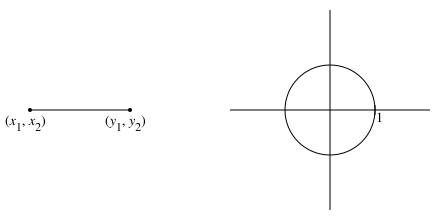
\includegraphics{Euclidean_metric}}
\end{center}
\caption{The Euclidean distance between $(x_1,x_2)$ and $(y_1,y_2)$ and the Euclidean unit circle in $\R^2$.}
\label{F:Euclidean_metric}
\end{figure}
Using this metric, the distance between two points $(x_1,x_2)$ and $(y_1,y_2)$ is the length of the segment connecting the points, while the unit circle (the set of points a distance 1 from the origin) looks like what we think of as a circle as illustrated in Figure \ref{F:Euclidean_metric}.

As we will see, there are many other metrics that can be defined on $\R^n$, or on other sets. 

 
\begin{pa} Consider the function $d_T$ that assigns to each pair of points in $\R^2$ the real number 
\[d_T((x_1,x_2),(y_1,y_2)) = | x_1-y_1 | + | x_2-y_2 |.\] 
This function $d_T$ is sometimes called the \emph{taxicab metric}\index{metric!taxicab} or \emph{distance} because the distance between points $x$ and $y$ can be thought of as obtained by driving around a city block rather than going directly from point $x$ to point $y$. 

Any distance function should satisfy certain properties: the distance between two points should never be negative, the distance from point $A$ to point $B$ should be the same as the distance from point $B$ to point $A$, the shortest distance between two points $A$ and $B$ should never be more than the distance from $A$ to some point $C$ plus the distance from $C$ to $B$, and the distance between points should only be zero if the points are the same. In this activity, we determine if $d_T$ has these properties. Let $x=(x_1,x_2)$ and $y=(y_1,y_2)$ in $\R^2$. 

\be
\item Prove that $d_T(x,y) \geq 0$. 

\item Prove that $d_T(x,y) = d_T(y,x)$. 

\item  Prove that $d_T(x,y) = 0$ if and only if $x = y$. 

\item Let $z = (z_1,z_2)$ in $\R^2$. Read the proof of Lemma \ref{lem:abs_TI} (below) and then use Lemma \ref{lem:abs_TI} to show that 
\[d_T(x,y) \leq d_T(x,z) + d_T(z,y).\]	
(Do you have any questions about the proof of the lemma?)

\begin{lemma} \label{lem:abs_TI} Let $a$ and $b$ be real numbers. Then
\[| a+b | \leq | a | + | b |.\]
\end{lemma}

\begin{proof} Let $a$ and $b$ be real numbers. To prove the lemma we consider cases. 
\begin{description}
\item[Case 1: $a \geq 0$ and $b \geq 0$.] In this case $a+b$ is nonnegative and so $| a | = a$, $| b | = b$, and $| a+b | = a+b$. Then
\[| a+b | = a+b =  | a | + | b |.\]
\item[Case 2: $a \leq 0$ and $b \leq 0$.] In this case $a = -a'$ and $b = -b'$ where $a'$ and $b'$ are nonnegative. It follows from Case 1 that 
\[| a+b | = | -(a'+b') | = | a'+b' | = a'+b' = | a' | + | b' | = | -a' | + | -b' | = | a | + | b |.\]
\item[Case 3: One of $a$ or $b$ is positive and the other negative.] Without loss of generality we assume $a > 0$ and $b < 0$. Again we consider cases. Note that $b < 0$ implies $a+b < a$. 
	\begin{itemize}
	\item Suppose $b \geq -2a$. Then $a+b \geq -a$ and so $-a \leq a+b < a$. It follows that  
\[| a+b | \leq a = | a | < | a | + | b |.\]  
	\item The last case is when $b < -2a$. In this case $-b > 2a$ and so 
	\[| b | = -b > 2a = 2| a | > | a |.\]
	 Then $a+b < a = | a | < | b |$. Finally, $a > 0$ implies $a+b > b = -| b |$. So
\[- | b | < a+b < | b |\]
and 
\[| a+b | \leq | b | < | a | + | b |.\]
	\end{itemize}
\end{description}
This proves our lemma for every possible pair $a$, $b$.
\end{proof}  

\item A picture to illustrate the taxicab distance $d_T$ between (points $x_1,x_2)$ and $(y_1,y_2)$ is shown in Figure \ref{F:PA_metric}. Draw a picture of the unit circle (the set of points a distance 1 from the origin) using the Taxicab metric. Explain your reasoning.
\begin{figure}[ht]
\begin{center}
\resizebox{!}{2.0in}{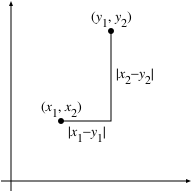
\includegraphics{Taxicab}}
\end{center}
\caption{The taxicab distance between $(x_1,x_2)$ and $(y_1,y_2)$ in $\R^2$.}
\label{F:PA_metric}
\end{figure}

	
\ee


\end{pa}

\begin{comment}

\ActivitySolution

\be
\item Since $| a | \geq 0$ for any $a \in \R$, we have that $| x_1-y_1 | \geq 0$ and $| x_2-y_2 | \geq 0$. Thus,
\[d_T(x,y) = | x_1-y_1 | + | x_2-y_2 | \geq 0.\]

\item  Since $| -1 | = 1$, we have that 
\begin{align*}
d_T(x,y) &= | x_1-y_1 | + | x_2-y_2 | \\
	&= | (-1)(y_1-x_1) | + | (-1)(y_2-x_2) | \\
	&= | (-1) | | y_1-x_1 | + | (-1) | | y_2-x_2 | \\
	&= | y_1-x_1 | + | y_2-x_2 | \\
	&= d_T(y,x).
\end{align*}


\item  Suppose 
\[d_T(x,y) =  | x_1-y_1 | + | x_2-y_2 | = 0.\]
Since $|a| \geq 0$ for every real number $a$, it follows that 
\[| x_1-y_1 | = 0 = | x_2-y_2 |.\]
Therefore, $x_1=y_1$ and $x_2=y_2$, which makes $x = y$. 

Now suppose $x = y$. Then $x_1=y_1$ and $x_2=y_2$ and 
\[| x_1-y_1 | = 0 = | x_2-y_2 |.\]
it follows that   
\[d_T(x,y) = | x_1-y_1 | + | x_2-y_2 | = 0+0 = 0.\]  

\item   First note that 
\begin{align*}
d(x,z) + d(z,y) &= \left(| x_1-z_1 | + | x_2-z_2 | \right) + \left( | z_1-y_1 | +  | z_2-y_2 | \right) \\
	&= \left(| x_1-z_1 | + | z_1-y_1 | \right) + \left( | x_2-z_2 |  + | z_2-y_2 | \right).
\end{align*}
Applying Lemma \ref{lem:abs_TI} give us 
\begin{align*}
d(x,z) + d(z,y) &= \left( | x_1-z_1 | + | z_1-y_1 | \right) + \left(| x_2-z_2 |  + | z_2-y_2 | \right) \\
	&\geq \left(| (x_1-z_1) + (z_1-y_1) | \right) + \left(| (x_2-z_2) + (z_2-y_2) | \right) \\
	&= | x_1-y_1 | + | x_2-y_2 | \\
	&= d(x,y).
\end{align*}

\item A point $(x_1,x_2)$ will be a distance 1 from the origin if $|x_1| + |x_2| = 1$. This will only happen if 
\[|x_2| = 1- |x_1| \text{ and } -1 \leq x_1, x_2 \leq 1.\]
In other words, the point $(x_1,x_2)$ must lie on one of the lines 
\begin{align*}
x_2 &= 1-x_1 \text{ if } x_1, x_2 \geq 0 \\
x_2 &= 1+x_1 \text{ if } x_1<0 \text{ and } x_2 \geq 0 \\
x_2 &= -1+x_1 \text{ if } x_1\geq 0 \text{ and } x_2 < 0 \\
x_2 &= -1-x_1 \text{ if } x_1, x_2 \leq 0.
\end{align*}
So the unit circle using the metric $d_T$ in $\R^2$ looks as depicted in Figure \ref{F:taxicab_circle}.
\begin{figure}[ht]
\begin{center}
\resizebox{!}{2.0in}{\includegraphics{Taxicab_circle}}
\end{center}
\caption{The unit circle in $\R^2$ using the taxicab metric.}
\label{F:taxicab_circle}
\end{figure}
	
\ee


\end{comment}

The taxicab metric can be extended to $\R^n$ for any $n \geq 1$ as follows. If $x = (x_1, x_2, \ldots, x_n)$ and $y = (y_1, y_2, \ldots, y_n)$ are in $\R^n$, then the taxicab distance $d_T(x,y)$ from $x$ to $y$ is defined as
\[d_T(x,y) = |x_1-y_1| + |x_2-y_2| + \cdots + |x_n-y_n| = \sum_{i=1}^n |x_i-y_i|.\]


\csection{Metric Spaces}

For most of our mathematical careers our mathematics has taken place in $\R^2$, where we measure the distance between points $(x_1,x_2)$ and $(y_1,y_2)$ with the standard Euclidean distance $d_E$. In our preview activity we saw that the function $d_T$ satisfies many of the same properties as $d_E$. These properties allow us to use $d_E$ or $d_T$ as distance functions. We call any distance function a \emph{metric}, and any space on which a metric is defined is called a \emph{metric space}. 

\begin{definition} A \textbf{metric}\index{metric} on a space $X$ is a function $d : X \times X \to \R^+ \cup \{0\}$ that satisfies the properties: 
\begin{enumerate}
\item $d(x,y) \geq 0$ for all $x,y \in X$,
\item $d(x,y) = 0$ if and only if $x = y$ in $X$,
\item $d(x,y) = d(y,x)$ for all $x, y \in X$, and
\item $d(x,y) \leq d(x,z) + d(z,y)$ for all $x,y,z \in X$.
\end{enumerate}
\end{definition}

Properties 1 and 2 of a metric say that a metric is \emph{positive definite}, while property 3 states that a metric is \emph{symmetric}. Property 4 of the definition is usually the most difficult property to verify for a metric and is called the \emph{triangle inequality}\index{triangle inequality}. 

\begin{definition} A \textbf{metric space}\index{metric space} is a pair $(X,d)$, where $d$ is a metric on the space $X$. 
\end{definition}

When the metric is clear from the context, we just refer to $X$ as the metric space.


\begin{activity} \label{act:MS_metrics} For each of the following, determine if $(X,d)$ is a metric space. If $(X,d)$ is a metric space, explain why. If $(X,d)$ is not a metric space, determine which properties of a metric $d$ satisfies and which it does not. If $(X,d)$ is a metric space, give a geometric description of the unit circle (the set of all points in $X$ a distance $1$ from the zero element) in the space.  
	\ba
	\item $X = \R$, $d(x,y) = \max\{|x|,|y|\}$. 

	
	\item $X = \R$, $d(x,y) = \begin{cases} 0 & \text{ if } x=y \\ 1 & \text{ if } x \neq y. \end{cases}$


	\item $X = \R^2$, $d((x_1,x_2),(y_1,y_2)) = \max\{| x_1-y_1 |, | x_2-y_2 | \}$ 

 
	\item $X = C[0,1]$, the set of all continuous functions on the interval $[0,1]$, 
	\[d(f,g) = \ds \int_0^1 | f(x) - g(x) | \, dx.\] 

	\ea

\end{activity}

\begin{comment}

\ActivitySolution

	\ba
	\item  This function $d$ is not a metric on $\R$. It is the case by definition that $d(x,y) \geq 0$ for all $x,y \in \R$. If $x \neq y$, then at least one of $x,y$ is not 0 and $d(x,y) > 0$. Also, $d(1,1) = 1$, not 0, so $d$ does not satisfy the second property of a metric. This $d$ is symmetric, and also satisfies the triangle inequality. To see why the triangle inequality is satisfied, let $x,y,z \in \R$. We look at two cases. 
\begin{itemize}
\item If $|x| \geq |z|$, then 
\[d(x,z)=|x| \text { and } d(x,y)+d(y,z) \geq |x| + d(y,z) \geq |x| = d(x,z).\]
\item If $|x| < |z|$, then 
\[d(x,z)=|z| \text { and } d(x,y)+d(y,z) \geq d(x,y) + |z| \geq |z| = d(x,z).\]
\end{itemize}
In either case,
\[d(x,z) \leq d(x,y)+d(y,z)\]
and $d$ satisfies the triangle inequality.
	
	\item This $d$ does define a metric on $X$. By definition, $d(x,y) \geq 0$ for all $x, y \in X$. If $x \neq y$, then $y \neq x$, so $d$ is symmetric. By definition, $d(x,y) = 0$ if and only if $x=y$. Let $x,y,z \in X$. Then 
$d(x,y)+d(x,z) = 0$ if and only if $x = y = z$. In this case
\[0 = d(x,z) = 0 + 0 = d(x,y) = d(y,z).\]
If $x$, $y$, and $z$ are not all equal, then 
\[d(x,y) + d(y,z) \geq 1 \geq d(x,z).\]
So $d$ satisfies the triangle inequality and $d$ is a metric. Note that this argument did not depend on the elements of $X$, so this $d$ defines a metric on any set. It is interesting to notice that the unit circle in this metric is all of $\R$ except for the origin. 

	\item Let $x = (x_1,x_2)$ and $y = (y_1, y_2)$. Now $|a| \geq 0$ for any real number $a$, so $d(x,y) \geq 0$. That $d$ is symmetric follows from the fact that $|-a| = |a|$ for any real number $a$:
	\[d(x,y) =\max\{ | x_1 - y_1 |, | x_2 - y_2 | \} = \max\{| y_1 - x_1 |, | y_2 - x_2 |\} = d(y,x).\]
If $x = y$, then 
\[d(x,y) =\max\{ | x_1 - y_1 |, | x_2 - y_2 | \} = \max\{0,0\} = 0.\]
If $d(x,y) = 0$, then
\[0 = 	\max\{ | x_1 - y_1 |, | x_2 - y_2 | \}.\]
But if $x_1 \neq y_1$ or $x_2 \neq y_2$, then $|x_1-y_1| > 0$ or $|x_2 - y_2 | > 0$, forcing $d(x,y) > 0$. So if $d(x,y) = 0$, then $x = y$. 

Now we consider the triangle inequality. Let $x = (x_1,x_2)$, $y=(y_1, y_2)$, $z = (z_1, z_2)$ in $\R^2$. We know that 
\[|x_1-z_1| = |(x_1-y_1) + (y_1-z_1)| \leq |x_1-y_1| + |y_1-z_1|\]
and
\[|x_2-z_2| = |(x_2-y_2) + (y_2-z_2)| \leq |x_2-y_2| + |y_2-z_2|.\]

It is the case that $d(x,z) = \max\{|x_1-z_1|,|x_2-z_2|\}$ is either equal to $|x_1-z_1|$ or $|x_2-z_2|$. Suppose that $d(x,z) = |x_1-z_1|$. Then 
\[d(x,z) \leq |x_1-y_1| + |y_1-z_1| \leq \max\{|x_1-y_1|, |x_2-y_2|\} + \max\{|y_1-z_1|, |y_2-z_2|\} = d(x,y) + d(y,z).\]
Similarly, if $d(x,z) = |x_2-z_2|$. Then 
\[d(x,z) \leq |x_2-y_2| + |y_2-z_2| \leq \max\{|x_1-y_1|, |x_2-y_2|\} + \max\{|y_1-z_1|, |y_2-z_2|\} = d(x,y) + d(y,z).\]
So $d$ satisfies the triangle inequality. Thus, $d$ is a metric on $X$. This metric is called the \emph{max} metric. In this case, the unit circle is the set of points $(x_1,x_2)$ such that $\max\{|x_1|, |x_2|\} = 1$. This is the set of points $(x_1,x_2)$ where $x_1 = 1$ and $-1 \leq x_2 \leq 1$ or $x_2 = 1$ and $-1 \leq x_1 \leq 1$. In other words, the unit circle in this space is the square centered at the origin of side length 2. 

	\item We show that $d$ is a metric. Let $f, g$ be in $C[0,1]$. If we integrate a nonnegative function over any interval, the resulting area is never negative. So $d(f,g) \geq 0$. Since $|a - b| = |b - a|$ for any real numbers $a$ and $b$, it follows that $d$ is symmetric. From calculus we know that 
	\[d(f,f) = \int_0^1 |f(x)-f(x)| \, dx = \int_0^1 0 \, dx = 0.\]
	Now suppose that $d(f,g) = 0$. To show that $f = g$, we proceed by contradiction and assume that $f \neq g$. So there exists $c \in [0,1]$ such that $f(c) \neq g(x)$. Since $f$ and $g$ are continuous, there must be some small interval $I$ in $[0,1]$ containing $c$ such that $f(x) \neq g(x)$ on $I$. Then ${f(x) - g(x)} > 0$ on $I$ and 
	\[\int_I |f(x) - g(x)| \, dx > 0.\]
Therefore,	
	\[d(f,g) = \int_0^1 |f(x)-g(x)| \, dx = \int_{x \notin I} |f(x)-g(x)| \, dx + \int_{x \in I} |f(x)-g(x)| \, dx > 0.\]
So $d(f,g) = 0$ implies that $f=g$. 

Finally, we consider the triangle inequality. Let $h \in C[0,1]$. Then
\begin{align*}
\int_0^1 |f(x)-g(x)| \, dx &= \int_0^1 |(f(x)-h(x))+(h(x)-g(x)| \, dx \\
	&\leq \int_0^1 |f(x)-h(x)| + |h(x)-g(x)| \, dx \\
	&= \int_0^1 |f(x)-h(x)| \, dx + \int_0^1 |h(x)-g(x)| \, dx \\
	&= d(f,h) + d(h,g).
\end{align*}	 

The unit circle is difficult to visualize here, but it is the set of functions $f$ that bound one unit of area between the graph of $f$ and the $x$-axis on $[0,1]$. 
	\ea

\end{comment}


It should be noted that not all metric spaces are infinite. We discuss one metric on a finite space in the following example.

\begin{example} \label{exp:finite_ms} Let $X = \{a,b,c\}$ and define $d: A \times A \to \R^+ \cup \{0\}$ with the entries in Table \ref{T:finite_metric_ex}.
\begin{table}[ht]
\begin{center}
\begin{tabular}{c|ccc}
	&$a$ 	&$b$		&$c$ \\ \hline
$a$	&$0$		&$3$		&$5$ \\ 
$b$	&$3$		&$0$		&$4$ \\
$c$	&$5$		&$4$		&$0$ 
\end{tabular}
\caption{Table of values for a function $d$.}
\label{T:finite_metric_ex}
\end{center}
\end{table}
By definition we have $d(x,y) \geq 0$ for all $x, y \in X$ with $d(x,y) = 0$ if and only if $x=y$. Since the table is symmetric around the diagonal, we can see that $d(x,y) = d(y,x)$ for all $x,y \in X$. The only item to verify is the triangle inequality. If $d(x,y) = 0$, then
\[d(x,y) = 0 \leq d(x,z) + d(z,y)\]
for any $x,y \in X$. If $d(x,z) = 0$, then $x=z$ and 
\[d(x,y) = d(z,y) \leq d(z,z) + d(z,y).\]
That leaves three cases to consider, when $x$, $y$, and $z$ are distinct. Now 
\begin{align*}
d(a,b) &= 3 \leq 5+4 = d(a,c) + d(c,b), \\
d(a,c) &= 5 \leq 3+4 = d(a,b) + d(b,c), \\
d(b,c) &= 4 \leq 3+5 = d(b,a) + d(a,c).
\end{align*}
So $d$ is a metric on $X$. 
\end{example}

Example \ref{exp:finite_ms} shows that even finite sets can be metric spaces. In fact, we can make a finite metric space by taking any finite subset $S$ of a metric space $(X,d)$ and use as a metric the restriction of $d$ to $S$. Example \ref{exp:finite_ms} illustrates this by letting $a = (0,0)$, $b = (3,0)$, and $c = (3,4)$ in $\R^2$. Then $d$ is the restriction of the Euclidean metric to the set $X$. Another way to construct a finite metric space is to start with a finite set of points and make a graph with the points as vertices. Construct edges so that the graph is connected (that is, there is a path from any one vertex to any other) and give weights to the edges as illustrated in Figure \ref{F:Graph_metric}. We then define a metric $d$ on $S$ by letting $d(x,y)$ be the length of a shortest path between vertices $x$ and $y$ in the graph. For example, $d(b,c) = d(b,e) + d(e,c) = 9$ in this example. 
\begin{figure}[h]
\begin{center}
\resizebox{!}{2.0in}{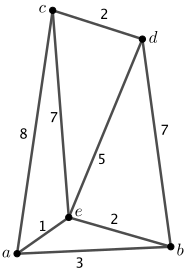
\includegraphics{Graph_metric.eps}}
\caption{A graph to define a metric.} 
\label{F:Graph_metric}
\end{center}
\end{figure}
%\includegraphics[trim=left bottom right top, clip]{file}

Just as with the Euclidean and taxicab metrics, item (c) in Activity \ref{act:MS_metrics} can be extended to $\R^n$ as follows. If $x = (x_1, x_2, \ldots, x_n)$ and $y = (y_1, y_2, \ldots, y_n)$ are in $\R^n$, then the maximum distance $d_M(x,y)$ from $x$ to $y$ is defined as
\[d_M(x,y) = \max\{| x_1-y_1 |, | x_2-y_2 |, |x_3-y_3|, \ldots, |x_n-y_n| \} = \max_{1 \leq i \leq n} \{|x_i-y_i|\}.\]
The metric $d_M$ is called the \emph{max} metric{\index{metric!max}. In the following section we prove that the Euclidean metric is in fact a metric. Proofs that $d_T$ and $d_M$ are metrics are left to Exercises (\ref{ex:Taxicab}) and (\ref{ex:Max}). 

\csection{The Euclidean Metric on $\R^n$}
The metric space that is most familiar to us is the metric space $(\R^2, d_E)$, where 
\[d_E((x_1,x_2), (y_1,y_2)) = \sqrt{(x_1-y_1)^2 + (x_2-y_2)^2}\] 
The metric $d_E$ called the \emph{standard} or \emph{Euclidean}\index{metric!Euclidean} metric on $\R^2$. 

We can generalize this Euclidean metric from $\R^2$ to any dimensional real space. Let $n$ be a positive integer and let $x = (x_1, x_2, \ldots, x_n)$ and $y = (y_1, y_2, \ldots, y_n)$ be in $\R^n$. We define $d_E : \R^n \times \R^n \to \R$ by 
\[d_E(x,y) = \sqrt{(x_1-y_1)^2 + (x_2-y_2)^2 + \cdots (x_n-y_n)^2} = \sqrt{\sum_{i=1}^n (x_i-y_i)^2}.\]
In the next activity we will show that $d_E$ satisfies the first three properties of a metric.  

\begin{activity} Let $x = (x_1, x_2, \ldots, x_n)$ and $y = (y_1, y_2, \ldots, y_n)$ be in $\R^n$.
\ba
\item Show that $d_E(x,y) \geq 0$. 

\item Show that $d_E(x,y) = d_E(y,x)$.

\item Show that if $x=y$, then $d_E(x,y) = 0$.

\item Show that if $d_E(x,y) = 0$, then $x=y$. 

\ea

\end{activity}

\begin{comment}

\ActivitySolution

\ba
\item Since $(x_i-y_i)^2 \geq 0$ for each $i$, we have 
\[d_E(x,y) =  \sqrt{\sum_{i=1}^n (x_i-y_i)^2} \geq 0.\] 

\item Since $(x_i-y_i)^2 = (y_i-x_i)^2$ for each $i$, we have 
\[d_E(x,y) =  \sqrt{\sum_{i=1}^n (x_i-y_i)^2} = \sqrt{\sum_{i=1}^n (y_i-x_i)^2} = d_E(y,x).\] 

\item If $x = y$, then $x_i = y_i$ and $x_i-y_i = 0$ for each $i$ . Then
\[d_E(x,y) =  \sqrt{\sum_{i=1}^n (x_i-y_i)^2} =  \sqrt{\sum_{i=1}^n 0} = 0.\] 

\item Suppose $d_E(x,y) = 0$. If $x_k \neq y_k$ for some $k$, then $(x_k - y_k)^2 > 0$. This makes
\[d_E(x,y) =  \sqrt{\sum_{i=1}^n (x_i-y_i)^2} =  \sqrt{\sum_{i \neq k} (x_i-y_i)^2 + (x_k-y_k)^2} \geq \sqrt{0 +  (x_k-y_k)^2} > 0.\]
So we must have $x_i = y_i$ for every $i$ and $x=y$. 

\ea

\end{comment}

Proving that the triangle inequality is satisfied is often the most difficult part of proving that a function is a metric. We will work through this proof with the help of the Cauchy-Schwarz Inequality. 

\begin{lemma}[Cauchy-Schwarz Inequality\index{Cauchy-Schwarz Inequality}] \label{lem:CS_Euclidean} Let $n$ be a positive integer and $x = (x_1, x_2, \ldots, x_n)$, $y=(y_1, y_2, \ldots, y_n)$ be in $\R^n$. Then 
\begin{equation} \label{eq:SL}
\sum_{i=1}^n x_iy_i \leq  \left(\sqrt{\sum_{i=1}^n x_i^2}\right) \left(\sqrt{\sum_{i=1}^n y_i^2}\right).
\end{equation} 
\end{lemma}

\begin{activity} Before we prove the Cauchy-Schwarz Inequality, let us analyze it in two specific situations.
	\ba
	\item Let $x=(1,4)$ and $y = (3,2)$ in $\R^2$. Verify the Cauchy-Schwarz Inequality in this case.

	\item Let $x=(1,2, -3)$ and $y = (-4, 0, -1)$ in $\R^3$. Verify the Cauchy-Schwarz Inequality in this case.

	\ea
\end{activity}

\begin{comment}

\ActivitySolution
	\ba
	\item Here we have 
	\[\sum_{i=1}^2 x_iy_i = (1)(3) + (4)(2) = 11\]
	and
	\[\left(\sqrt{\sum_{i=1}^2 x_i^2}\right) \left(\sqrt{\sum_{i=1}^2 y_i^2}\right) = \sqrt{1+9}\sqrt{16+4} = \sqrt{200} \approx 14.1.\]

	\item Here we have 
	\[\sum_{i=1}^3 x_iy_i = (1)(-4) + (2)(0) + (-3)(-1) = -1\]
	and
	\[\left(\sqrt{\sum_{i=1}^3 x_i^2}\right) \left(\sqrt{\sum_{i=1}^3 y_i^2}\right) = \sqrt{1+4+9}\sqrt{16+0+1} = \sqrt{238} \approx 15.4.\]

	\ea

\end{comment}

Now we prove the Cauchy-Schwarz Inequality.

\begin{proof}[Proof of the Cauchy-Schwarz Inequality]  Let $n$ be a positive integer and $x = (x_1, x_2, \ldots, x_n)$, $y=(y_1, y_2, \ldots, y_n)$ be in $\R^n$. To verify (\ref{eq:SL}) it suffices to show that 
\[\left(\sum_{i=1}^n x_iy_i\right)^2 \leq  \left(\sum_{i=1}^n x_i^2\right) \left(\sum_{i=1}^n y_i^2\right).\]
This is difficult to do directly, but there is a nice trick one can use.
Consider the expression
\[\sum (x_i-\lambda y_i)^2.\]
(All of our sums are understood to be from 1 to $n$, so we will omit the limits on the sums for the remainder of the proof.) Now
\begin{align}
0 & \leq \sum (x_i-\lambda y_i)^2 \notag \\
	&= \sum \left(x_i^2 - 2\lambda x_iy_i + \lambda^2 y_i^2 \right) \notag \\
	&= \left( \sum y_i^2 \right)\lambda^2 - 2\left(\sum x_iy_i\right) \lambda + \left(\sum x_i^2\right). \label{eq:SL_1}
\end{align}
To interpret this last expression more clearly, let $a=\sum y_i^2$, $b=-2\sum x_iy_i$ and $c = \sum x_i^2$. The inequality defined by (\ref{eq:SL_1}) can then be written in the form
\[p(\lambda) = a \lambda^2 + b \lambda + c \geq 0.\]
So we have a quadratic $p(\lambda)$ that is never negative. This implies that the quadratic $p(\lambda)$ can have at most one real zero. The quadratic formula gives the roots of $p(\lambda)$ 
as
\[\frac{-b \pm \sqrt{b^2-4ac}}{2a}.\]
If $b^2-4ac > 0$, then $p(\lambda)$ has two real roots. Therefore, in order for $p(\lambda)$ to have at most one real zero we must have
\[0 \geq b^2-4ac = 4 \left(\sum x_iy_i\right)^2 - 4\left(\sum y_i^2\right)\left(\sum x_i^2\right)\]
or
\[\left(\sum y_i^2\right)\left(\sum x_i^2\right) \geq \left(\sum x_iy_i\right)^2.\]
This establishes the Cauchy-Schwarz Inequality.
\end{proof}

One consequence of the Cauchy-Schwarz Inequality that we will need to show that $d_E$ is a metric is the following.

\begin{corollary} \label{cor:SL} Let $n$ be a positive integer and $x = (x_1, x_2, \ldots, x_n)$, $y=(y_1, y_2, \ldots, y_n)$ be in $\R^n$. Then 
\[\sqrt{\sum_{i=1}^n (x_i+y_i)^2} \leq \sqrt{\sum_{i=1}^n x_i^2} + \sqrt{\sum_{i=1}^n y_i^2}.\]
\end{corollary}

\begin{activity} Before we prove the corollary, let us analyze it in two specific situations.
	\ba
	\item Let $x=(1,4)$ and $y = (3,2)$ in $\R^2$. Verify Corollary \ref{cor:SL} in this case.
 
	\item Let $x=(1,2, -3)$ and $y = (-4, 0, -1)$ in $\R^3$. Verify Corollary \ref{cor:SL} in this case.

	\ea
\end{activity}

\begin{comment}

\ActivitySolution

	\ba
	\item Here we have 
	\[\sqrt{\sum_{i=1}^2 (x_i+y_i)^2} = \sqrt{4^2+6^2} = \sqrt{52} \approx 7.2\]
	and
	\[\sqrt{\sum_{i=1}^2 x_i^2} + \sqrt{\sum_{i=1}^2 y_i^2} = \sqrt{1+16} + \sqrt{9+4} = \sqrt{17}+\sqrt{13} \approx 7.7.\] 
 
	\item Here we have 
	\[\sqrt{\sum_{i=1}^3 (x_i+y_i)^2} = \sqrt{(-3)^1+2^2+(-4)^2} = \sqrt{29} \approx 5.4\]
	and
	\[\sqrt{\sum_{i=1}^3 x_i^2} + \sqrt{\sum_{i=1}^3 y_i^2} = \sqrt{1+4+9} + \sqrt{16+0+1} = \sqrt{14}+\sqrt{17} \approx 7.8.\] 


	\ea
	
\end{comment}

Now we prove Corollary \ref{cor:SL}.

\begin{proof}[Proof of Corollary \ref{cor:SL}] Let $n$ be a positive integer and $x = (x_1, x_2, \ldots, x_n)$, $y=(y_1, y_2, \ldots, y_n)$ be in $\R^n$. Now
\begin{align*}
\sum \left(x_i+y_i\right)^2 &= \sum \left(x_i^2 +2x_iy_i + y_i^2 \right) \\
	&= \sum x_i^2 + 2\sum x_iy_i + \sum y_i^2 \\
	&\leq \sum x_i^2 + 2\left(\sqrt{\sum x_i^2}\right) \left(\sqrt{\sum y_i^2} \right) + \sum y_i^2 \\
	&= \left(\sqrt{\sum x_i^2} + \sqrt{\sum y_i^2}\right)^2.
\end{align*}
Taking the square roots of both sides yields the desired inequality.
\end{proof}

We can now complete the proof that $d_E$ is a metric.

\begin{activity} Let $n$ be a positive integer and $x = (x_1, x_2, \ldots, x_n)$, $y=(y_1, y_2, \ldots, y_n)$, and $z=(z_1, z_2, \ldots, z_n)$ be in $\R^n$. Use Corollary \ref{cor:SL} to show that 
\[d_E(x,y) \leq d_E(x,z)+d_E(z,y).\]

\end{activity}

\begin{comment}

\ActivitySolution Now we can apply Corollary \ref{cor:SL} to verify that $d_E$ satisfies the triangle inequality.  Let $n$ be a positive integer and $x = (x_1, x_2, \ldots, x_n)$, $y=(y_1, y_2, \ldots, y_n)$ be in $\R^n$. Then
\begin{align*}
d_E(x,z) + d_E(z,y) &= \sqrt{\sum (x_i-z_i)^2} + \sqrt{\sum (z_i-y_i)^2} \\
	&\geq \sqrt{ \sum \left[(x_i-z_i)+(z_i-y_i)\right]^2}  \\
	&= \sqrt{ \sum (x_i-y_i)^2}  \\
	&= d_E(x,y).
\end{align*}

\end{comment}


This concludes our proof that the Euclidean metric is in fact a metric. 

We have seen several metrics in this section, some of which are given special names. Let $x = (x_1, x_2, \ldots, x_n)$ and $y = (y_1, y_2, \ldots, y_n)$
\begin{itemize}
\item The Euclidean metric $d_E$, where
\[d_E(x,y) = \sqrt{(x_1-y_1)^2 + (x_2-y_2)^2 + \cdots (x_n-y_n)^2} = \sqrt{\sum_{i=1}^n (x_i-y_i)^2}.\]
\item The Taxicab metric $d_T$, where 
\[d_T(x,y) = |x_1-y_1| + |x_2-y_2| + \cdots + |x_n-y_n| = \sum_{i=1}^n \{|x_i-y_i|\}.\]
\item The max metric $d_M$, where 
\[d_M(x,y) = \max\{| x_1-y_1 |, | x_2-y_2 |, |x_3-y_3|, \ldots, |x_n-y_n| \} = \max_{1 \leq i \leq n} \{|x_i-y_i|\}.\]
\end{itemize}
We have only shown that $d_T$ and $d_M$ are metrics on $\R^2$, but similar arguments apply in $\R^n$. Proofs are left to Exercises (\ref{ex:Taxicab}) and (
\ref{ex:Max}). In addition, the \emph{discrete metric}\index{metric!discrete}
\[d(x,y) = \begin{cases} 0 & \text{ if } x=y \\ 1 & \text{ if } x \neq y \end{cases}\]
makes any set $X$ into a metric space. The proof is left to Exercise (\ref{ex:MS_discrete}).

\csection{Summary}
Important ideas that we discussed in this section include the following.
\begin{itemize}
\item A metric on a space $X$ is a function that measures distance between elements in the space. More formally, a metric on a space $X$ is a function $d: X \times X \to \R^+ \cup \{0\}$ such that 
	\begin{enumerate}
	\item $d(x,y) \geq 0$ for all $x,y \in X$,
	\item $d(x,y) = 0$ if and only if $x = y$ in $X$,
	\item $d(x,y) = d(y,x)$ for all $x, y \in X$, and
	\item $d(x,y) \leq d(x,z) + d(z,y)$ for all $x,y,z \in X$.
	\end{enumerate}
A metric space is any space combined with a metric defined on that space.

\item The Euclidean, taxicab, and max metric are all metrics on $\R^n$, so they all provide ways to measure distances between points in $\R^n$. These metric are different in how they define the distances. 

	\begin{itemize}
	\item The Euclidean metric is the standard metric that we have used through our mathematical careers. For elements $x = (x_1, x_2, \ldots, x_n)$ and $y = (y_1, y_2, \ldots, y_n)$ in $\R^n$, the Euclidean metric $d_E$ is defined as
\[d_E(x,y) =  \sqrt{(x_1-y_1)^2 + (x_2-y_2)^2 + \cdots (x_n-y_n)^2} = \sqrt{\sum_{i=1}^n (x_i-y_i)^2}.\]
With this metric, the unit circle in $\R^2$ (the set of points a distance $1$ from the origin) is the standard unit circle we know from Euclidean geometry. 

	\item The taxicab metric $d_T$ is defined as
\[d_T(x,y) = |x_1-y_1| + |x_2-y_2| + \cdots + |x_n-y_n| = \sum_{i=1}^n |x_i-y_i|.\]
The unit circle in $\R^2$ using the taxicab metric is the square with vertices $(1,0)$, $(0,1)$, $(-1,0)$, and $(0,-1)$ when viewed in Euclidean geometry. 

	\item The max metric $d_M$ is defined by 
\[d_M(x,y) = \max\{| x_1-y_1 |, | x_2-y_2 |, |x_3-y_3|, \ldots, |x_n-y_n| \} = \max_{1 \leq i \leq n} \{|x_i-y_i|\}.\]
Under the max metric, the unit circle in $\R^2$ is the square with vertices $(1,1)$, $(-1,1)$, $(-1,-1)$, and $(1,-1)$ when viewed in Euclidean geometry.

	\end{itemize}
	
\end{itemize}


\csection{Exercises}

\be

\item \label{ex:MS_discrete} Let $X$ be a set.  Show that the function $d$ (the discrete metric) defined by 
\[d(x,y) = \begin{cases} 0 & \text{ if } x=y \\ 1 & \text{ if } x \neq y \end{cases}\]
is a metric. 

\begin{comment}

\ExerciseSolution Let $x$, $y$, and $z$ be in $X$. By definition, $d(x,y) \geq 0$, $d(x,y) = 0$ if and only if $x=y$, and $d(x,y) = d(y,x)$. So the only item to prove is the triangle inequality. We consider the cases $x \neq y$ and $x = y$. 
\begin{itemize}
\item If $x \neq y$, then 
\[d(x,y) + d(y,z) \geq 1 \geq d(x,z).\]
\item If $x=y$, then 
\[d(x,y) + d(y,z) = d(y,z) = d(x,z).\]
\end{itemize}
We conclude that $d$ is a metric on any set. 

\end{comment}


\item \label{ex:MS_mod_metric} Let $X = \{1,3,5\} \subset \Z$ and define $d: X \times X \to \R$ by $d(x,y) = xy - 1 \pmod{n}$. That is, $d(x,y)$ is the remainder when $xy - 1$ is divided by $n$. 
	\begin{itemize}
	\item For each value of $n$, determine if $d$ defines a metric on $X$. Prove your answers. 
	\item The unit circle in $\R^2$ with metric $d$ is the set of all points in $\R^2$ whose distance from the origin is $1$. If we let the distance be less than $1$, then we have what we call an open ball. We can make this same definition in any metric space.
	
\begin{definition} \label{def:ms_open_ball} Let $(Y, d_Y)$ be a metric space.  For any positive real number $r$, the \textbf{open ball centered at}\index{open ball in a metric space} $b$ \textbf{of radius} $r$ in $(Y, d_Y)$ is the  the set 
\[B(b,r) = \{y \in Y \mid d_Y(y,b) < r\}.\]
\end{definition}

If $(X,d)$ is a metric space for a given value of $n$, determine all of the open balls in $X$ centered at $1$. If $(X,d)$ is not a metric space, explain why. 
	\end{itemize}

\ba
\item $n = 4$

\item $n = 8$

\ea

\begin{comment}

\ExerciseSolution

\ba
\item  Since $xy-1 \pmod{4}$ is never negative, we see that $d(x,y) \geq 0$ for all $x,y \in X$. To determine if $d(x,y) = 0$ if and only if $x=y$, we calculate all of the distances as shown in Table \ref{T:d_example_4}.
\begin{table}[h]
\begin{center}
\begin{tabular}{|c|c|c|c|} \hline
		&$1$	&$3$	&$5$	\\ \hline
$1$		&$0$	&$2$	&$0$	\\ \hline
$3$		&$2$	&$0$	&$2$	\\ \hline
$5$		&$0$	&$2$	&$0$	\\ \hline
\end{tabular}
\caption{Values of $d$ with $n=4$.}
\label{T:d_example_4}
\end{center}	
\end{table}
Note that $d(1,5)=0$, but $1 \neq 5$. Thus, $d$ is not a metric on $X$. 

\item  Since $xy-1 \pmod{8}$ is never negative, we see that $d(x,y) \geq 0$ for all $x,y \in X$. To verify that $d(x,y) = 0$ if and only if $x=y$, we calculate all of the distances as shown in Table \ref{T:d_example_8}.
\begin{table}[h]
\begin{center}
\begin{tabular}{|c|c|c|c|} \hline
		&$1$	&$3$	&$5$	\\ \hline
$1$	&$0$	&$2$	&$4$	\\ \hline
$3$	&$2$	&$0$	&$6$	\\ \hline
$5$	&$4$	&$6$	&$0$	\\ \hline
\end{tabular}
\caption{Values of $d$ with $n=8$.}
\label{T:d_example_8}
\end{center}	
\end{table}
The symmetry along the main diagonal in Table \ref{T:d_example_8} also shows that $d(x,y) = d(y,x)$ for all $x, y \in X$. 

Finally, we consider the triangle inequality. Let $a,b,c \in X$. If $a=b$, then 
\[d(a,b) = 0 \leq d(a,c) + d(c,b).\]
So we only need consider the cases where $a \neq b$. Assume $a \neq b$. If $c = a$, then 
\[d(a,b) = d(c,b) = d(a,c) + d(c,b).\]
A similar result holds if $c = b$. So the only case left to consider is if $a$, $b$, and $c$ are all distinct. In this case, $d(a,b) \leq 6$, while $d(a,c) + d(c,b) \geq 2 + 4 = 6$. So 
\[d(a,b) \leq 6 \leq 2 + 4 \leq d(a,c) + d(c,b).\]
Therefore, $d$ is a metric on $X$ and $(X,d)$ is a metric space. 


The open balls centered at $a=1$ in $X$ are 
\begin{align*}
B(1,r) &= \{1\} \text{ if } r \leq 2, \\
B(1,r) &= \{1,3\} \text{ if } 2 < r \leq 4, \\
B(1,r) &= \{1,3,5\} \text{ if } 4 < r. 
\end{align*}

\ea

\end{comment}


\item \label{ex:MS_Q_metric} Let $Q$ be the set of all rational numbers in reduced form. A rational number $\frac{r}{s}$ is in reduced form if $s > 0$ and $r$ and $s$ have no common factors larger than $1$. Define $d : Q \times Q \to \R$ by 
\[d\left(\frac{a}{b}, \frac{r}{s}\right) = \max\{| a-r |, | b-s |\}.\]
	\ba
	\item Prove that $d$ is a metric. 
	
	\item A metric allows us to determine which elements in our metric space are ''close" together. Describe the set of elements in $Q$ that are a distance no more than $1$ from $\frac{2}{3}$ using this metric $d$. In other words, describe the open ball centered at $\frac{2}{3}$ with radius $1$ (see Definition \ref{def:ms_open_ball}).
	
	\item If $a$, $b$, and $c$ are elements of a metric space $(X, d_X)$, we say that $b$ is between $a$ and $c$ if $d_X(a,c) = d_X(a,b) + d_X(b,c)$. Using the Euclidean metric on $\Q$, there are infinitely many different rational numbers between $0$ and $1$ (the rational numbers between $0$ and $1$ that lie on the Euclidean line through $0$ and $1$. Describe all of the points in $(\Q,d)$ that are between $0$ and $1$.  
	
	\ea

\begin{comment}

\ExerciseSolution

	\ba
	\item Let $\frac{a}{b}$ and $\frac{r}{s}$ be rational numbers in reduced form. By definition we have that $d\left(\frac{a}{b}, \frac{r}{s}\right) \geq 0$. Since $|r-a| = |a-r|$ and $|s-b| = |b-s$, it follows that 
	\[d\left(\frac{a}{b}, \frac{r}{s}\right) =  \max\{| a-r |, | b-s |\} =  \max\{| r-a |, | s-b |\} = d\left(\frac{r}{s}, \frac{a}{b}\right).\]
	So $d$ is symmetric. 
	
	Suppose $d\left(\frac{a}{b}, \frac{r}{s}\right) = 0$. Then $\max\{| a-r |, | b-s |\} = 0$ which implies that both $|a-r| = 0$ and $|b-s| = 0$. From this we have that $a=r$ and $b=s$, or $\frac{a}{b} = \frac{r}{s}$. Conversely, suppose $\frac{a}{b} = \frac{r}{s}$. The fact that $\frac{a}{b} = \frac{r}{s}$ means that $as = br$. Since $a$ and $b$ share no prime factors, every prime in the prime factorization of $b$ must be a factor of $s$. Thus, $s = \pm b$. But since $b$ and $s$ are positive, it follows that $b=s$.  Cancelling $b$ from both sides of $as = br$ yields $a=r$. But this means that $|a-r| = |b-s| = 0$ and so $d\left(\frac{a}{b}, \frac{r}{s}\right) = 0$.
	
Lastly, we must verify the triangle inequality. Let $\frac{e}{f}$ be another rational number in reduced form. By the triangle inequality of the Euclidean metric, we know that 
\[|a - e| \leq |a-r| + |r-e| \text{ and }  |b-f| \leq |b-s| + |s-f|.\]
Now 
\[d\left(\frac{a}{b}, \frac{r}{s}\right) =  \max\{| a-r |, | b-s |\} \geq |a-r| \text{ and } d\left(\frac{a}{b}, \frac{r}{s}\right) =  \max\{| a-r |, | b-s |\} \geq |b-s|\]
and
\[d\left(\frac{r}{s}, \frac{e}{f}\right) =  \max\{| r-e |, | s-f |\} \geq |r-e| \text{ and } d\left(\frac{r}{s}, \frac{e}{f}\right) =  \max\{| r-e |, | s-f |\} \geq |s-f|.\]
So 
\[d\left(\frac{a}{b}, \frac{r}{s}\right) + d\left(\frac{r}{s}, \frac{e}{f}\right) \geq |a-r| + |r-e| \geq |a-e|\]
and
\[d\left(\frac{a}{b}, \frac{r}{s}\right) + d\left(\frac{r}{s}, \frac{e}{f}\right) \geq |s-d| + |s-f| \geq |b-f|.\]
Therefore,
\[d\left(\frac{a}{b}, \frac{r}{s}\right) + d\left(\frac{r}{s}, \frac{e}{f}\right) \geq \max\{|a-e|, |b-f|\} = d\left(\frac{a}{b}, \frac{e}{f}\right).\]
We conclude that $d$ is a metric. 
		
	\item An element $\frac{a}{b}$ in $Q$ is within $\frac{1}{2}$ of $\frac{2}{3}$ if
	\[d\left(\frac{a}{b}, \frac{2}{3}\right) \leq 1.\]
	This happens when
	\[\max\{|a-2|, |b-3|\} \leq 1.\]
We must then have $|a-2| \leq 1$ and $|b-3| \leq 1$. Now $|a-2| \leq 1$ when $1 \leq a \leq 3$ and $|b-3| \leq 1$ when $2 \leq b \leq 4$.  But $a$ and $b$ must be integers so $a$ can be $1$, $2$, or $3$ and $b$ can be $2$, $3$, or $4$. But it must also be the case that $a$ and $b$ have no common positive factors other than $1$, so the elements in $Q$ that are no more than a distance $1$ from $\frac{2}{3}$ are $\frac{1}{2}$, $\frac{1}{3}$, $\frac{1}{4}$, $\frac{2}{3}$, $\frac{3}{2}$, and $\frac{3}{4}$. 

\item Since $0 = \frac{0}{1}$ and $1 = \frac{1}{1}$ we have that $d(0,1) = 1$. So if $b = \frac{u}{v}$ is between $0$ and $1$, then 
\[1 = d(0,b) + d(b,1).\]
Now $d(0,b) = \max\{|u|, |v-1|\}$ and $d(1,b) = \max\{|u-1|, |v-1|\}$. We consider the cases. 
\begin{itemize}
\item Suppose $d(0,b) = |u|$ and $d(a,b) = |u-1|$. Then 
\[1 = |u| + |u-1|.\]
Since $u$ is an integer, the cases are $|u| = 0$ and $|u-1| = 1$, or $|u|=1$ and $|u-1| = 0$. When $u=0$, $b=0$.  When $|u-1|=0$ we have $u = 1$. The fact that  $|u-1| \geq |v-1|$ implies that $0 \geq |v-1|$ and $v = 1$. In this case $b = 1$. 

\item Suppose $d(0,b) = |u|$ and $d(a,b) = |v-1|$. Then 
\[1 = |u| + |v-1|.\]
The cases are $|u|=0$ and $|v-1| = 1$, or $|u| = 1$ and $|v-1| = 0$.  When $u=0$, $b=0$. When $|v-1| = 0$ we must have $v = 1$. The fact that $0 = |v-1| \geq |u-1|$ implies that $u=1$. 

\item Suppose $d(0,b) = |v-1|$ and $d(a,b) = |u-1|$. Then 
\[1 = |v-1| + |u-1|.\]
The cases are $|u-1|=0$ and $|v-1| = 1$, or $|u-1| = 1$ and $|v-1| = 0$.  When $|u-1|=0$ we have $u=1$. The fact that $0 = |u-1| \geq |v-1|$ tells us that $v=1$. So $b=1$. When $|v-1| = 0$, then $v=1$. The fact that  $0 = |v-1| \geq |u|$ implies that $u=0$. This makes $b=0$. 

\item Suppose $d(0,b) = |v-1|$ and $d(a,b) = |v-1|$. Then 
\[1 = |v-1| + |v-1|.\]
But this is impossible when $v$ is an integer. 

\end{itemize}
We conclude that the only rational numbers in $(\Q,d)$ between $0$ and $1$ are $b = 0$ and $b=1$. 

	\ea
	

\end{comment}


\item Let $(\Q,d)$ be the metric space from Exercise (\ref{ex:MS_Q_metric}). If $a$, $b$, and $c$ are elements of a metric space $(X, d_X)$, we say that $b$ is \emph{between} $a$ and $c$ if $d_X(a,c) = d_X(a,b) + d_X(b,c)$. Using the Euclidean metric on $\Q$, there are infinitely many different rational numbers between $0$ and $1$ (the rational numbers between $0$ and $1$ that lie on the Euclidean line through $0$ and $1$. In this exercise we explore numbers that are between others in the space $(\Q,d)$. 

\ba

\item Find all of the elements in $(\Q,d)$ that are between $0$ and $1$.  

\item Which is closer to $0$ in $(\Q,d)$: $1$ or $\frac{1}{3}$?

\item Now find all of the elements in $(\Q,d)$ that are between $0$ and $\frac{1}{3}$.  

\ea
	

\begin{comment}

\ExerciseSolution

	\ba
\item Since $0 = \frac{0}{1}$ and $1 = \frac{1}{1}$ we have that $d(0,1) = 1$. So if $b = \frac{u}{v}$ is between $0$ and $1$, then 
\[1 = d(0,b) + d(b,1).\]
Now $d(0,b) = \max\{|u|, |v-1|\}$ and $d(1,b) = \max\{|u-1|, |v-1|\}$. We consider the cases. 
	\begin{itemize}
	\item Suppose $d(0,b) = |u|$ and $d(1,b) = |u-1|$. Then 
\[1 = |u| + |u-1|.\]
Since $u$ is an integer, the cases are $|u| = 0$ and $|u-1| = 1$, or $|u|=1$ and $|u-1| = 0$. When $u=0$, $b=0$.  When $|u-1|=0$ we have $u = 1$. The fact that  $|u-1| \geq |v-1|$ implies that $0 \geq |v-1|$ and $v = 1$. In this case $b = 1$. 

	\item Suppose $d(0,b) = |u|$ and $d(1,b) = |v-1|$. Then 
\[1 = |u| + |v-1|.\]
The cases are $|u|=0$ and $|v-1| = 1$, or $|u| = 1$ and $|v-1| = 0$.  When $u=0$, $b=0$. When $|v-1| = 0$ we must have $v = 1$. The fact that $0 = |v-1| \geq |u-1|$ implies that $u=1$. 

	\item Suppose $d(0,b) = |v-1|$ and $d(1,b) = |u-1|$. Then 
\[1 = |v-1| + |u-1|.\]
The cases are $|u-1|=0$ and $|v-1| = 1$, or $|u-1| = 1$ and $|v-1| = 0$.  When $|u-1|=0$ we have $u=1$. The fact that $0 = |u-1| \geq |v-1|$ tells us that $v=1$. So $b=1$. When $|v-1| = 0$, then $v=1$. The fact that  $0 = |v-1| \geq |u|$ implies that $u=0$. This makes $b=0$. 

	\item Suppose $d(0,b) = |v-1|$ and $d(a,b) = |v-1|$. Then 
\[1 = |v-1| + |v-1|.\]
But this is impossible when $v$ is an integer. 

	\end{itemize}
We conclude that the only rational numbers in $(\Q,d)$ between $0$ and $1$ are $b = 0$ and $b=1$. 

\item Since $d(0,1) = 1$ and $d\left(0,\frac{1}{3}\right) = 2$, it appears that in this space $1$ is closer to $0$ than $\frac{1}{3}$ is. 

\item We have that $d\left(0,\frac{1}{3}\right) = 2$. So if $b = \frac{u}{v}$ is between $0$ and $\frac{1}{3}$, then 
\[2 = d(0,b) + d\left(b,\frac{1}{3}\right).\]
Now $d(0,b) = \max\{|u|, |v-1|\}$ and $d\left(b,\frac{1}{3}\right) = \max\{|u-1|, |v-3|\}$. We consider the cases. 

\begin{itemize}
	\item Suppose $d(0,b) = |u|$ and $d\left(b,\frac{1}{3}\right) = |u-1|$. Then 
\[2 = |u| + |u-1|.\]
The cases are $|u| = 0$ and $|u-1| = 2$, $|u|=1$ and $|u-1| = 1$, and $|u|=2$ and $|u-1| = 0$.  But there are no integers $u$ for which $|u| = 0$ and $|u-1| = 2$, $|u|=1$ and $|u-1| = 1$, and $|u|=2$ and $|u-1| = 0$.
	
	\item Suppose $d(0,b) = |u|$ and $d\left(b,\frac{1}{3}\right) = |v-3|$. Then 
\[2 = |u| + |v-3|.\]
The cases are $|u|=0$ and $|v-3| = 2$, $|u| = 1$ and $|v-3| = 1$, and $|u|=2$ and $|v-3| = 0$. 
	\begin{enumerate}[i.]
	\item When $u=0$, $b=0$. 
	\item When $|u|=1$ and $|v-3| = 1$ we have $u =-1$ or $u=1$ and $v = 2$ or  $v=4$. The cases that satisfy $|u| \geq |v-1|$ and $|v-3| \geq |u-1|$ are $u=1$ and $v=2$. This makes $b = \frac{1}{2}$. 
	\item When $|u|=2$ and $|v-3| = 0$, we have $u = -2$ or $u = 2$ and $v = 3$. None of these cases satisfy $|u| \geq |v-1|$ and $|v-3| \geq |u-1|$. 
	\end{enumerate}

\end{itemize}
		
\item Suppose $d(0,b) = |v-1|$ and $d\left(b,\frac{1}{3}\right) = |u-1|$. Then 
\[2 = |v-1| + |u-1|.\]
The cases are $|u-1|=0$ and $|v-1| = 2$, $|u-1| = 1$ and $|v-1| = 1$, and $|u-1|=2$ and $|v-1| = 0$. 
	\begin{enumerate}[i.]
	\item When $|u-1|=0$ and $|v-1| = 2$, we have $u = 1$ and $v = 3$. This case satisfies both $|v-1| \geq |u|$ and $|u-1| \geq |v-3|$. So $b=\frac{1}{3}$. 
	\item When $|u-1|=1$ and $|v-1| = 1$ we have $u =0$ or $u=2$ and $v = 2$. When $u=0$, $b=0$. The case $u=2$ and $v=2$ doesn't satisfy both $|v-1| \geq |u|$ and $|u-1| \geq |v-3|$.  
	\item When $|u-1|=2$ and $|v-1| = 0$, we have $u = -1$ or $u = 3$ and $v = 1$. Neither case satisfies both $|v-1| \geq |u|$ and $|u-1| \geq |v-3|$.  
	\end{enumerate}
	
\item Suppose $d(0,b) = |v-1|$ and $d\left(b,\frac{1}{3}\right) = |v-3|$. Then 
\[2 = |v-1| + |v-3|.\]
The cases are $|v-1|=0$ and $|v-3| = 2$, $|v-1| = 1$ and $|v-3| = 1$, and $|v-1|=2$ and $|v-3| = 0$. 
	\begin{enumerate}[i.]
	\item The only time $|v-1|=0$ and $|v-3| = 2$ is when $v=1$. We must also have $|v-1| \geq |u|$ and $|v-3| \geq |u-1|$. This only happens when $u=0$. So $b=0$. 
	\item The only time $|v-1|=1$ and $|v-3| = 1$ is when $v=2$. We must also have $|v-1| \geq |u|$ and $|v-3| \geq |u-1|$. This only happens when $u=1$. So $b=\frac{1}{2}$. 
	\item The only time $|v-1|=2$ and $|v-3| = 0$ is when $v=3$. We must also have $|v-1| \geq |u|$ and $|v-3| \geq |u-1|$. This only happens when $u=1$. So $b=\frac{1}{3}$. 
		
	\end{enumerate}
	
We conclude that the rational numbers in $(\Q,d)$ between $0$ and $\frac{1}{3}$ are $b = 0$, $\frac{1}{3}$, and $\frac{1}{2}$.  It seems strange that $\frac{1}{2}$ should be between $0$ and $\frac{1}{3}$, but recall that $d\left(0, \frac{1}{3}\right) = 2$ while $d\left(0, \frac{1}{2}\right) = 1$. So $\frac{1}{3}$ is farther away from $0$ than $\frac{1}{2}$. 



	\ea


\end{comment}

\item \label{ex:Taxicab} Prove that the taxicab metric $d_T$ is a metric on $\R^n$. 

\begin{comment}

\ExerciseSolution Let $x = (x_1, x_2, \ldots, x_n)$ and $y = (y_1, y_2, \ldots, y_n)$ be in $\R^n$. Since $d_E(x_i,y_i) = |x_i-y_i|  \geq 0$ for each $i$, it follows that
\[d_T(x,y) = \sum_{i=1}^n | x_i-y_i | \geq 0.\]
We also know that $|r-s| = |s-r|$ for any $r, s \in \R$, so 
\[d_T(x,y) = \sum_{i=1}^n | x_i-y_i | = \sum_{i=1}^n | y_i-x_i | = d_T(y,x).\]

Suppose $x = y$. Then $x_i=y_i$ for each $i$ and 
\[d_T(x,y) = \sum_{i=1}^n | x_i-y_i | = \sum_{i=1}^n 0 = 0.\]

Conversely, if $d_T(x,y) = 0$, the facts that $|x_i - y_i| \geq 0$ and 
\[d_T(x,y) = \sum_{i=1}^n | x_i-y_i | = 0\]
imply that $|x_i-y_i| = 0$ for each $i$. Consequently, $x_i = y_i$ for each $i$ and $x = y$.

Now we address the triangle inequality. Let $z = (z_1, z_2, \ldots, z_n) \in \R^n$. Then
\begin{align*}
d_T(x,z) &=  \sum_{i=1}^n | x_i-z_i | \\
	&= \sum_{i=1}^n | (x_i-y_i) + (y_i-z_i) | \\
	&\leq \sum_{i=1}^n | (x_i-y_i) | + |(y_i-z_i) | \\
	&= \sum_{i=1}^n | (x_i-y_i) | + \sum_{i=1}^n |(y_i-z_i) | \\
	&= d_T(x,y) + d_T(y,z).
\end{align*}

\end{comment}

\item \label{ex:Max} Let $A$ and $B$ be nonempty finite subsets of $\R^n$, and let $A+B = \{a+b \mid a \in A, b \in B\}$.

\ba

\item Prove that $\max (A+B) \leq \max A + \max B$.

\item Prove that the max metric $d_M$ is a metric on $\R^n$. 

\ea

\begin{comment}

\ExerciseSolution 

\ba

\item Let $m = \max (A+B)$. Then $m = a+b$ for some $a \in A$ and $b \in B$. Now $a \leq \max A$ and $b \leq \max B$, so $m = a+b \leq \max A + \max B$. 

\item Let $x = (x_1, x_2, \ldots, x_n)$ and $y = (y_1, y_2, \ldots, y_n)$ be in $\R^n$. Since $d_E(x_i,y_i) = |x_i-y_i|  \geq 0$ for each $i$, it follows that
\[d_M(x,y) = \max\{ | x_i-y_i | \} \geq 0.\]
We also know that $|r-s| = |s-r|$ for any $r, s \in \R$, so 
\[d_M(x,y) = \max\{ | x_i-y_i | \} = \max\{ | y_i-x_i | \} = d_M(y,x).\]

Suppose $x = y$. Then $x_i=y_i$ for each $i$ and 
\[d_M(x,y) = \max\{ | x_i-y_i | \} = 0.\]

Conversely, if $d_M(x,y) = 0$, the fact that $|x_i - y_i| \geq 0$ for each $i$ implies that we must have $|x_i-y_i| = 0$ for each $i$. Consequently, $x_i = y_i$ for each $i$ and $x = y$.

Now we address the triangle inequality. Let $z = (z_1, z_2, \ldots, z_n) \in \R^n$. From part (a) we then have
\begin{align*}
d_M(x,z) &= \max\{ | x_i-z_i | \} \\
	&= \max\{ | (x_i-y_i) + (y_i-z_i) | \} \\
	&\leq \max\{ |x_i-y_i| + |y_i-z_i| \} \\
	&\leq \max \{(x_i-y_i) |\} + \max\{|(y_i-z_i) | \} \\
	&= d_M(x,y) + d_M(y,z).
\end{align*}

\ea

\end{comment}

\item \label{ex:MS_hub} If $x = (x_1, x_2, \ldots, x_n)$, we let $|x| = \sqrt{x_1^2+x_2^2+ \cdots + x_n^2}$. For $x = (x_1, x_2, \ldots, x_n)$ and $y = (y_1, y_2, \ldots y_n)$, define $d_H: \R^n \times \R^n \to \R$ by 
\[d_H(x,y) = \begin{cases} 0 &\text{ if } x=y \\ |x|+|y| &\text{ otherwise}. \end{cases}\]

\ba
\item Show that $d_H$ is a metric (called the \emph{hub} metric). 

\item ~
	\begin{enumerate}[i.]
	\item  Let $a = \left(\frac{1}{2}, 0\right)$. Explicitly describe which points are in the set $B(a,1)$ in $(\R^2, d_H)$. (See Exercise \ref{ex:MS_mod_metric} for the definition of an open ball.)

	\item Let $a = (3,4)$. Explicitly describe which points are in the set $B(a,1)$ in $(\R^2, d_H)$. 

	\item Now explicitly describe all open balls in $(\R^2, d_H)$. 
		
	\end{enumerate}

\ea

\begin{comment}

\ExerciseSolution

\ba
\item Let $x$ and $y$ be in $\R^n$. 
\begin{itemize}
\item Note that $d_H(x,y) \geq 0$ by definition. 
\item If $x=y$, then $d_H(x,y) = 0 = d_H(y,x)$. If $x \neq y$, then 
\[d_H(x,y) = |x|+|y| = |y|+|x| = d_H(y,x).\]
\item Next we demonstrate that $d_H(x,y) = 0$ if and only if $x=y$. First, suppose $x=y$. Then $d_H(x,y) = 0$ by definition. Now suppose that $d_H(x,y) = 0$. This means that $|x|+|y| = 0$. Since $|x| \geq 0$ and $|y| \geq 0$, it follows that $|x| = |y| = 0$. If $x = (x_1,x_2, \ldots, x_n)$, then $0 = |x| = \sqrt{x_1^2+x_2^2 + \cdots + x_n^2}$ implies that $x_i = 0$ for each $i$ and so $x = 0$. For the same reason, $y = 0$. So if $d_H(x,y) = 0$, then $x = y = 0$. 
\item To verify the triangle inequality, let $z$ be in $\R^2$. We know that $|y| \geq 0$, so 
\[d_H(x,z) = |x| + |z| \leq |x| + 2|y| + |z| = (|x|+|y|) + (|y|+|z|) = d_H(x,y) + d_H(y,z).\]
\end{itemize}

\item ~
	\begin{enumerate}[i.]
	\item  We look for all points $x$ in $\R^2$ such that $d(x,a) < 1$. That is, the set of points $x$ such that $|x| + |a| < 1$. Now $|a| = \frac{1}{2}$, so we look for the set of points $x$ in $\R^2$ such that $|x| < 1-\frac{1}{2} = \frac{1}{2}$. If $x = (x_1,x_2)$, we then want all of the points satisfying $|x|^2 = x_1^2+x_2^2 < \frac{1}{4}$. This set of points satisfying $x_1^2+x_2^2 = \frac{1}{4}$ is the Euclidean circle centered at the origin of radius $\frac{1}{2}$. So 
\[B(a,1) = \{a\} \cup \left\{(x_1,x_2) \mid x_1^2+x_2^2 < \left(\frac{1}{2}\right)^2\right\}\]
is the point $a$ along with the open Euclidean disk of radius $\frac{1}{2}$ centered at the origin as illustrated in Figure \ref{F:Hub_metric}.
\begin{figure}[h]
\begin{center}
\resizebox{!}{2.0in}{\includegraphics{Hub_metric.png}}
\caption{The open ball $B(a,1)$.} 
\label{F:Hub_metric}
\end{center}
\end{figure}

	\item Notice that $|a| = \sqrt{3^2+4^2} = \sqrt{25} = 5$. So if $x \in B(a,1)$, then 
\[d_H(x,a) = |x|+|a| = |x| + 5 < 1.\]
Bu this makes $|x| < -4$, which is not possible. So $B(a,1) = \{a\}$. 

	\item Let $a \in \R^2$, and let $r > 0$. Then $x \in B(a,r)$ when 
\[d_H(x,a) = |x| + |a| < r\]
or $B(a,r)$ is the set consisting of $a$ and of all $x \in \R^2$ such that 
\[|x| < r - |a|.\]
If $r-|a| \leq 0$, then the only point in $B(a,r)$ is $a$. If $r > |a|$, then $B(a,r)$ is the open Euclidean disk centered at the origin of radius $r - |a|$ along with the point $a$.  Note that if $|a| < r \leq 2|a|$, then $r - |a| \leq |a|$ and so $a$ is not in the open Euclidean ball centered at the origin of radius $r$. But when $r \geq 2|a|$, then $a$ is in this disk. 
	
	\end{enumerate}
	
\ea

\end{comment}


\item Let $\Z$ be the set of integers and let $p$ be a prime. For each pair of distinct integers $m$ and $n$ there is an integer $t = t(m,n)$ such that $|m-n| = k \times p^t$, where $p$ does not divide $k$. For example, if $p=5$, $m = 34$, and $n = 7$, then $m-n = 27 = 27 \times 5^0$. So $t(43,7) = 27$. However, if $m = 54$ and $n = 4$, then $m-n = 50 = 2 \times 5^2$. So $t(54,4) = 2$. 

Define $d: \Z \times \Z \to \R$ by 
\[d(m,n) = \begin{cases} 0 &\text{ if } m=n \\ \frac{1}{p^t} &\text{ if } m \neq n. \end{cases}\] 


\ba

\item Determine the values of $d(62,170)$ using $p=3$ and $d(14008,2003)$ using $p=7$. 

\item Prove that if $a$, $b$, and $c$ are in $\Z$, then 
\[t(a,c) \geq \min\{t(a,b), t(b,c)\}.\]

\item Prove that $(\Z,d)$ is a metric space.

\item Let $p = 3$. Describe the set of all elements $x$ in $(\Z,d)$ such that $d(x,0) = 1$. 

\item Continue with $p=3$. Describe the set of all elements $x$ in $(\Z,d)$ such that $d(x,0) < \frac{1}{2}$.

\ea

\begin{comment}

\ExerciseSolution

\ba

\item With $p=3$ we have $170-62 = 108 = 4 \times 3^3$, so $t(62,170) = 3$. This makes $d(62,170) = \frac{1}{27}$.  

With $p=7$, we have $14008-2003 = 12005 = 5 \times 7^4$, so $t(2003,14008) = 4$. This makes $d(14008,2003) = \frac{1}{7^4}$. 

\item Let $p$ be prime and let $a$, $b$, and $c$ be in $\Z$. We have that 
\[a-c = k_1p^{t(a,c)}, \ a-b = k_2p^{t(a,b)}, \ \text{ and } \ b-c = k_3p^{t(b,c)}\]
for some integers $k_1$, $k_2$, and $k_3$ that are not divisible by $p$. Then
\[k_1p^{t(a,c)} = a-c = (a-b) + (b-c) = k_2p^{t(a,b)} +  k_3p^{t(b,c)}.\]
We consider the cases where $t(a,b) \leq t(b,c)$ and $t(a,b) > t(b,c)$.
\begin{description}
\item[Case 1: $t(a,b) \leq t(b,c)$.] Then $\min\{t(a,b), t(b,c)\} = t(a,b)$. It follows that
\[a-c = k_2p^{t(a,b)} +  k_3p^{t(b,c)} = p^{t(a,b)}\left(k_2 + k_3p^{t(b,c) - t(a,b)}\right)\]
and so $p^{t(a,b)}$ divides $a-c$. This makes $t(a,c) \geq t(a,b)$. 
\item[Case 2: $t(a,b) < t(b,c)$.] Then $\min\{t(a,b), t(b,c)\} = t(b,c)$. It follows that
\[a-c = k_2p^{t(a,b)} +  k_3p^{t(b,c)} = p^{t(b,c)}\left(k_3p^{t(a,b) - t(b,c)} + k_3\right)\]
and so $p^{t(b,c)}$ divides $a-c$. This makes $t(a,c) \geq t(b,c)$. 
\end{description}
In either case we have $t(a,c) \geq \min\{t(a,b), t(b,c)\}$. 


\item Let $p$ be a prime and let $a$ and $b$ be integers. Since $p$ is prime, $p^t$ is positive for any real integer $t$. Thus, $d(a,b) \geq 0$. 

If $a=b$, then $d(a,b) = 0 = d(b,a)$. If $a \neq b$, then $a-b = k \times p^t$ and $b-a = (-k) \times p^t$. Then $d(a,b) = \frac{1}{p^t} = d(b,a)$. so $d$ is symmetric.

If $a = b$, then $d(a,b) = 0$ by definition. Now suppose that $d(a,b) = 0$. If $a \neq b$, then $d(a,b) = \frac{1}{p^t} \neq 0$, which is a contradiction. Therefore, $a = b$. We conclude that $d(a,b) = 0$ if and only if $a=b$. 

Finally, we verify the triangle inequality. Let $c \in \Z$.  If $a = b$, then 
\[d(a,b) = 0 \leq d(a,c) + d(c,b).\]
So assume $a \neq b$. If $c = a$, then 
\[d(a,b) = 0 + d(a,b) = d(a,c) + d(c,b)\]
and if $c = b$, then 
\[d(a,b) = d(a,b) + 0 = d(a,c) + d(c,b).\]
So we can assume that $a$, $b$, and $c$ are three distinct integers. Let $m = \min\{t(a,b), t(b,c)\}$. Note that if $m \leq n$ for some nonnegative integer $n$, then $p^m \leq p^n$ and $\frac{1}{p^m} \geq \frac{1}{p^n}$. From (a) we know that $m \leq t(a,c)$, so we have 
\[d(a,b) + d(b,c) = \frac{1}{p^{t(a,b)}} + \frac{1}{p^{t(b,c)}} \geq \frac{1}{p^m} \geq \frac{1}{p^{t(a,c)}} = d(a,c).\]

\item Let $p=3$ and let $a \in \Z$ such that $d(a,0) = 1$. Then $a = a-0 = k \times p^1$ for some integer $k$. So the set of integers $a$ such that $d(a,0) = 1$ are all of the integers of the form $kp$ where $\gcd(k,p) = 1$.  

\item Note that $t(a,b)$ is always a nonnegative integer. So if $d(a,0) < \frac{1}{2}$, then $d(a,0) = 0$. This is the set of all integers relatively prime to $p$. 

\ea


\end{comment}



\item Let $(X, d_X)$ and $(Y, d_Y)$ be metric spaces. We can make the Cartesian product $X \times Y$ into a metric space by defining a metric $d'$ on $X \times Y$ as follows. If $(x_1, y_2)$ and $(x_2, y_2)$ are in $X \times Y$, then 
	\[d'((x_1,y_1), (x_2, y_2)) = \max\{d_X(x_1,x_2), d_Y(y_1,y_2)\}.\]
You may assume without proof that $d'$ is a metric on $X \times Y$. 

\ba
\item Let $(X, d_X) = (\R^2, d_M)$ and $(Y, d_Y) = (\R^2, d_T)$. Let $u = ((1,2), (1,-1))$ and $v = ((0,5),(2,-2))$. What is 
\[d'(u,v)?\]
Recall that 
\[d_M((x_1,x_2),(y_1,y_2)) = \max\{ | x_1-y_1 |, | x_2-y_2 |\}\]
and
\[d_T((x_1,x_2),(y_1,y_2)) = | x_1-y_1 | + | x_2-y_2 |.\]
		
\item Let $(X, d_X) = (\R, d_E)$ and $(Y, d_Y) = (\R, d)$, where $d$ is the discrete metric. Let  
\[A=\{(x,y) \in \R \times \R \mid -1\leq x \leq 1 \text{ and } -1 \leq y \leq 1\}\]
in $X \times Y$.  Let $a = (0,1)$ in $X \times Y$. Describe, geometrically, what the open ball $B(a,1)$ looks like in the product space $X \times Y$.  Draw a picture of this open ball. %Is $a$ an interior point of $A$? Explain. 

\ea

\begin{comment}

\ExerciseSolution
		\ba
		\item  In this case we have 
\begin{align*}
d'(((1,2), (1,-1)), &((0,5),(2,-2))) = \max\{d_M((1,2), (0,5)), d_T((1,-1), (2,-2))\} \\
	&= \max\{\max\{| 1-0 |, | 2-5 |\}, | 1-2 | + | -1-(-2) |\} \\
	&= \max\{3, 1+1 \} \\
	&= 3.
\end{align*}
	
		\item  If $y \neq 1$, then $d(y,1) = 1$ and $d'((x,y), a) \geq 1$. So the points in $B(a,1)$ lie along the line $y=1$. Now
\[d'((x,1),a) = d_E(x,0) = | x |,\]
so $B(a,1)$ is the open line segment $\{(x,y) \mid -1<x<1, y=1\}$. See Figure \ref{F:Open_product}
Since $B(a,1) \subseteq A$, the point $a$ is an interior point of $A$. 
\begin{figure}[h]
\begin{center}
\resizebox{!}{2.0in}{\includegraphics{Open_product.pdf}}
\caption{The open ball $B(a,1)$.} 
\label{F:Open_product}
\end{center}
\end{figure}

		\ea

\end{comment}

\item Let $X = \R^+$, the set of positive reals, and define $d: X \times X \to \R$ by 
\[d(x,y) = |\ln(y/x)|.\]
Is $d$ is a metric on $X$? Prove your answer. 

\begin{comment}

\ExerciseSolution We show that $d$ is a metric on $X$. Let $x, y \in X$. By definition we have $d(x,y) \geq 0$. Also,
\[d(x,y) = |\ln(y/x)| = |\ln(x/y)^{-1}| = |-\ln(x/y)| = |\ln(x/y)| = d(y,x).\]

Suppose $x=y$. Then $d(x,y) = |\ln(1)| = 0$. Conversely, suppose $d(x,y) = 0$. Then $|\ln(y/x)| = 0$. This implies that $\frac{y}{x} = 1$ or that $x=y$. 

Finally, we verify the triangle inequality. Let $z \in X$. Then
\begin{align*} 
d(x,y) + d(y,z) &= |\ln(y/x)| + |\ln(z/y)| \\
	&= |\ln(y) - \ln(x)| + |\ln(z) - \ln(y)| \\
	&= |\ln(x) - \ln(y)| + |\ln(y) - \ln(z)| \\
	&\geq |\ln(x) - \ln(z)| \\
	&= d(x,z).
\end{align*}

We conclude that $d$ is a metric on $X$. 

\end{comment}

\item \label{ex:1_over_1_plus_t_metric} Let $d: \R \times \R \to \R$ be defined by 
\[d(x,y) = \frac{|x-y|}{|x-y|+1}.\]
Show that $d$ is a metric on $\R$. (Hint: For the triangle inequality, note that $d(x,y) = f(|x-y|)$ where $f(t) = \frac{t}{t+1}$, and $f$ is an increasing function.)

\begin{comment}

\ExerciseSolution Let $x, y, z \in \R$. By definition, $d(x,y) \geq 0$. Also, 
\[d(x,y) = \frac{|x-y|}{|x-y|+1} = \frac{|y-x|}{|y-x|+1} = d(y,x).\]

If $x=y$, then $|x-y| = 0$ and $d(x,y) = 0$. Conversely, if $d(x,y) = 0$, then it follows that $|x-y| = 0$ or $x=y$. 

Finally, we demonstrate the triangle inequality. Let $f(t) = \frac{t}{t+1}$. Then $d(x,z) = f(|x-z|)$. Since $f'(t) = \frac{1}{(t+1)^2} > 0$ when $t > 0$, we see that $f$ is an increasing function. So
\begin{align*}
d(x,z) &= f(|x-z|)    \\
	&= f(|(x-y)+(y-z)|) \\
	&\leq f(|x-y|+|y-z|) \\
	&= \frac{|x-y|+|y-z|}{(|x-y|+|y-z|+1)} \\
	&= \frac{|x-y|}{(|x-y|+|y-z|+1)} + \frac{|y-z|}{(|x-y|+|y-z|+1)} \\
	&\leq \frac{|x-y|}{(|x-y|+1)} + \frac{|y-z|}{(|y-z|+1)} \\
	&= d(x,y) + d(y,z).
\end{align*}
We conclude that $d$ is a metric. 

Note that $d(x,y) < 1$ for all $x,y \in \R$. This is an example of a \emph{bounded} metric. 

\begin{definition} A metric $d$ on a set $X$ is \textbf{bounded} if there is a constant $K$ such that $d(x,y) \leq K$ for all $x, y \in X$.
\end{definition} 
 
\end{comment}

\item Let $(X,d)$ be a metric space and $k$ be a constant. Define $kd: X \times X \to \R$ by 
\[(kd)(x,y) = kd(x,y).\]
Under what, if any, conditions is $kd$ a metric on $X$. Justify your answer. 


\item A real valued function $f$ on an interval is \emph{concave} if 
\begin{equation} \label{eq:concave}
f((1-\alpha)x + \alpha y) \geq (1-\alpha)f(x) + \alpha f(y)
\end{equation}
for all $\alpha \in [0,1]$ and all $x$ and $y$ in the interval. Note that the expression $(1-\alpha)x + \alpha y$ is linear in $\alpha$ and is equal to $x$ when $\alpha = 0$ and $y$ when $\alpha = 1$. So $(1-\alpha)x + \alpha y$ is a parameterization of the line segment joining $x$ to $y$. As Figure \ref{F:concave} indicates, (\ref{eq:concave}) implies that the graph of a concave function $f$ on any interval $[x,y]$ lies above the secant line joining the points $(x,f(x))$ and $(y,f(y))$. 
\begin{figure}[ht]
\begin{center}
\resizebox{!}{1.75in}{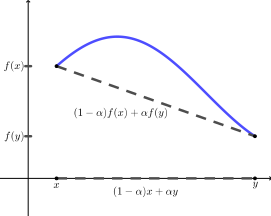
\includegraphics{Concave}}
\caption{A concave function.}
\label{F:concave}
\end{center}
\end{figure}

\ba

\item Let $f(x) = -x^2$ map $\R$ to $\R$ with the standard Euclidean metric. Show that $f$ is concave on the interval $[-1,1]$.  (Hint: Start with the fact that $\alpha(1-\alpha)(x-y)^2 \geq 0$.)

\item Show that if $f$ is a concave function on $[0,\infty)$ and $f(0) \geq 0$, an interval and $a$ and $b$ are in the interval, then 
\[f(a) + f(b) \geq f(a+b).\]
(Hint: Consider (\ref{eq:concave}) with $y=0$. Then use the fact that $\frac{a}{a+b}$ is in $[0,1]$.)

\item Suppose $(X,d)$ is a metric space and $f: [0, \infty) \to [0, \infty)$ is an increasing, concave function such that $f(x) = 0$ if and only if $x=0$. Prove that $f \circ d$ is a metric on $X$. 

\ea

\begin{comment}

\ExerciseSolution 

\ba

\item Let $x$ and $y$ be in $[-1,1]$ and let $\alpha$ be between $0$ and $1$. Since $\alpha$ and $1-\alpha$ are both between $0$ and $1$, and $(x-y)^2 \geq 0$, we have that 
\begin{align*}
\alpha(1-\alpha)(x-y)^2 &\geq 0 \\
(\alpha-\alpha^2)(x^2-2xy+y^2)  &\geq 0 \\
\alpha(x^2-2xy+y^2) - \alpha^2(x^2-2xy+y^2) &\geq 0 \\
\alpha x^2 - \alpha^2x^2 - 2 \alpha xy + 2\alpha^2xy - \alpha^2y^2 + \alpha y^2 &\geq 0 \\
 \big( -x^2 +2 \alpha x^2 - \alpha^2 x^2 -  2 \alpha xy + 2\alpha^2xy - \alpha^2y^2 \big)  + (x^2 - \alpha x^2 + \alpha y^2) &\geq 0 \\
  \big( -(1-\alpha)^2x^2 - 2\alpha(1-\alpha)xy - \alpha^2y^2 \big) + (x^2 - \alpha x^2 + \alpha y^2) &\geq 0 \\
  -((1-\alpha)x + \alpha y)^2 -((1-\alpha)(-x^2) + \alpha (-y^2)) &\geq 0 \\
f((1-\alpha)x + \alpha y) - ((1-\alpha)f(x) + \alpha f(y)) &\geq 0  \\
f((1-\alpha)x + \alpha y)  &\geq (1-\alpha)f(x) + \alpha f(y).
\end{align*}

So $f$ is concave on $[-1,1]$. Note that this argument doesn't depend on $x$ and $y$ begin in the interval $[-1,1]$, so $f$ is concave on any interval. 

\item First note that if $y=0$ we have 
\[f(tx) \geq tf(x) + (1-t) f(y) \geq tf(x)\]
for all $x \in [0,\infty)$ and all $t \in [0,1]$. 
Let $a, b \in [0, \infty)$ with $a \neq b$. Then 
\[f(a)+f(b) = f\left(\frac{a}{a+b}(a+b)\right) + f\left(\frac{b}{a+b}(a+b)\right) \geq \frac{a}{a+b}f(a+b) + \frac{a}{a+b}f(a+b) = f(a+b).\]

\item Let $x, y, z \in X$. Since the codomain of both $f$ and $d$ is the set of non-negative real numbers, we conclude that $(f \circ d)(x,y) \geq 0$. Also,
\[(f \circ d)(x,y) = f(d(x,y)) = f(d(y,x)) = (f \circ d)(y,x)\]
and $f \circ d$ is symmetric. 

Suppose $x=y$. Then 
\[(f \circ d)(x,y) = f(d(x,x)) = f(0) = 0.\]
Conversely, suppose $(f \circ d)(x,y) = 0$. Then $f(d(x,y)) = 0$. The fact that $f(t) = 0$ if and only if $t=0$ implies that $d(x,y) = 0$. Thus, $x=y$. 

Finally, we address the triangle inequality. The result of part (a) and the fact that $f$ is increasing show that  
\begin{align*}
(f \circ d)(x,y) + (f \circ d)(y,z) &= f(d(x,y)) + f(d(y,z)) \\
	&\geq f(d(x,y)+d(y,z)) \\
	&\geq f(d(x,z) \\
	&= (f \circ d)(x,z).
\end{align*}

\ea

\end{comment}



\item For each of the following, answer true if the statement is always true. If the statement is only sometimes true or never true, answer false and provide a concrete example to illustrate that the statement is false. If a statement is true, explain why. 
	\ba
	\item The function $d: \R \times \R \to \R$ defined by $d(x,y) = (x-y)^2$ is a metric on $\R$. 

	\item Every nonempty set can be made into a metric space. 
	
	\item It is possible to define an infinite number of metrics on every set containing at least two elements.

	\item Let $(X, d_X)$ and $(Y, d_Y)$ be metric spaces with $|X| \geq 2$. Then the function $d: X \times Y \to \R$ defined by $d((a,b),(c,d)) = d_X(a,c)d_Y(b,d)$ is a metric on $X \times Y$.
	
	\item Let $(X,d)$ be a metric space. If $X$ is infinite, then the range of $d$ is also an infinite set. 

			
	\ea

\begin{comment}

\ExerciseSolution

	\ba
	
	\item This statement is false. Although $d$ satisfies $d(x,y) \geq 0$ and $d(x,y) = d(y,x)$ for all $x$, $y$ in $\R$, and $d(x,y) = 0$ if and only if $x=y$, the function $d$ fails to satisfy the triangle inequality. Note that $d(1,3) = 2^2 = 4$ but 
	\[d(1,2) + d(2,3) = 1^2+1^2 = 2 < d(1,3).\]
	
		\item This statement is true. The discrete metric is a metric on any set. 
	
	\item This statement is true. If $d$ is a metric on a set $X$ and $k$ is a positive real number, then $kd : X \times X \to \R$ defined by $(kd)(x,y) = k(d(x,y))$ is also a metric. To see why, let $x$, $y$, and $z$ be in $X$
	\begin{itemize}
	\item The fact that $d(x,y) \geq 0$ implies that $kd(x,y) \geq 0$. 
	\item Since $d(x,y) = d(y,x)$ it is also the case that $kd(x,y) = kd(y,x)$.
	\item Because $d(x,x) = 0$ we also have $kd(x,x) = 0$, and if $kd(x,y) = 0$, then $d(x,y) = 0$ which makse $x = y$.
	\item Finally $kd$ satisfies the triangle inequality:
	\[(kd)(x,z) = k(d(x,z)) \leq k(d_x,y) + d(y,z)) = kd(x,y) + kd(y,z) = (kd)(x,y) + (kd)(y,z).\]
	\end{itemize}
	
	\item This statement is false. Let $x_1$ and $x_2$ be distinct elements in $X$ and let $y \in Y$. Then
	\[d((x_1,y), (x_2,y)) = d_X(x_1,x_2)d_Y(y,y) = 0\]
	even though $(x_1,y) \neq (x_2,y)$. 
		
	\item This statement is false. Let $X = \R$ with the discrete metric. Then the range of $d$ is $\{0,1\}$. 

	
	\ea


\end{comment}

\ee
  %3
\achapter{4}{Applications of Metric Spaces} \label{chap:metric_spaces_apps}

\csection{Introduction}\label{sec_met_space_app}

In this section we explore two applications of metric spaces.  

\csection{The Hamming Metric}\label{sec_hamming}

In our society, a great deal of information is communicated electronically. Bank transactions, television programs, military communications, cell phone calls, digital images, and almost any interchange one can think of either can be or is digitized and transmitted electronically. In many situations we need to compare one set of data to another (e.g., Internet searches for text strings or image matches, DNA strands), and metrics are often used for this purpose. Computers work in a binary system, that is they recognize only zeros and ones. So a digital text message is a string of zeros and ones. That is, a digital message is a collection of  elements in the space $X^n$ for some positive integer $n$, where $X = \{0,1\}$. Each element in $X^n$ is called a \emph{word} - that is, a word is an element in $X^n$ denoted in the form $(x_1, x_1, \ldots, x_n)$. Just like in the English language, where not every combination of letters corresponds to words that make sense, not every word is recognizable as part of an intelligible message. We might, for example, code the letters of the alphabet by assigning numbers 1-26 to the letters, then make them elements of $X^n$ by converting to binary. The collection of all intelligible words is called a \emph{code}. So a code is just some subset of $X^n$ that all parties agree are sensible words. The words in a code are called \emph{code words}. To deal with problems that occur in transmitting digital messages, like scrambling (\emph{encoding}) messages, unscrambling (\emph{decoding}) messages, and detecting and correcting errors in messages, it is useful to have a way to measure distance between words. One way is to use the Hamming metric. 

\begin{definition} Let $x = (x_1, x_2, \ldots, x_n)$ and $y = (y_1, y_2, \ldots, y_n)$ be words in $X^n$. The \textbf{Hamming distance} \index{metric!Hamming} $d_H$ between $x$ and $y$ is 
\[d_H(x,y) = \sum_{i=1}^n | x_i-y_i |.\]
\end{definition}

Recall that for each $i$ both $x_i$ and $y_i$ are either 0 or 1. So 
\[| x_i-y_i | = \begin{cases} 0 &\text{if } x_i=y_i \\ 1 &\text{ if } x_i \neq y_i. \end{cases}\]
In other words, $d_H(x,y)$ counts the number of components at which $x$ and $y$ are different.

\begin{activity} ~

\ba 
\item Explain why $d_H$ is a metric.

\item Suppose we create a code
\[C = \{c_1,c_2,c_3,c_4,c_5,c_6,c_7,c_8\}\] 
in $X^6$, where  
\begin{center}
\begin{tabular}{lll}
$c_1 = (0,0,0,0,0,0)$, 	&$c_2=(0,0,0,0,1,1)$, 	&$c_3=(0,0,0,1,0,1)$, 	\\
$c_4=(0,0,1,0,0,1)$, 		&$c_5=(0,0,0,1,1,0)$, 	&$c_6=(0,0,1,0,1,0)$, 	\\
$c_7=(0,0,1,1,0,0)$, 		&$c_8=(0,0,1,1,1,1)$.	&
\end{tabular}
\end{center}
That is, the words $c_1$, $c_2$, $c_3$, $c_4$, $c_5$, $c_6$, $c_7$, $c_8$ are the only words that can comprise a message. 

Find $d_H(c_2, c_8)$.

\item Suppose we are on the receiving end of the message 
\begin{equation*} \label{eq:message}
(0,0,0,1,1,1) \ (0,0,1,1,0,0) \ (1,0,0,0,0,0) \ (0,0,0,0,1,1) \ (0,0,1,0,0,1).
\end{equation*} 
	\begin{enumerate}[i.]
	\item How do we know that an error has occurred in transmission of the message we received?

	\item To correct the errors in this received message, we replace the incorrect words with the code word(s) in $C$ closest to them. Correct this message. (Note that there may be more than one possible substitution. Find all of the possibilities.)
	
		\end{enumerate}
	
\ea

\end{activity}

\begin{comment}

\ActivitySolution

\ba

\item Note that $d_H$ is just the taxicab metric on $X^n$ and so the same argument that shows the taxicab metric is a metric on $\R^n$ will work in $X^n$. 

	\begin{enumerate}[i.]
	\item Since $c_2$ and $c_8$ differ only in the third and fourth components, we have that $d_H(c_2,c_8) = 2$. 

	\item  Note that $(0,0,0,1,1,1)$ and $(1,0,0,0,0,0)$ are not in $C$. Since $C$ contains all of the possible words in our message, we know that there are errors in our message. 

	\item 
	\begin{itemize}
	\item The code words closest to $(0,0,0,1,1,1)$ are $c_2$, $c_3$, $c_5$, and $c_8$, which are all a distance $1$ from $(0,0,0,1,1,1)$. 
	\item The code word closest to $(1,0,0,0,0,0)$ is $c_1$, which is a distance $1$ from $(0,0,0,1,0,0)$.
	\end{itemize}
So the messages that are closest to the one received are $c_i \ c_7 \ c_1 \ c_2 \ c_4$, where $i$ is one of $2$, $3$, $5$, or $8$. We assume that one of these is the correct message.	

	\end{enumerate}

\ea

\end{comment}

\csection{The Levenshtein Metric}\label{sec_levenshtein}

The Levenshtein metric is one measure of distance that researchers use to understand DNA. DNA is composed of double chains of nucleotides, which wind together to form a double helix. The nucleotides come in four types: adenine (A), cytosine (C), guanine (G), and thymine (T). The nucleotides in the two chains of a DNA strand pair together, (A with T, and C with G), so the nucleotides in one chain determine the nucleotides in the other. Therefore, we can represent a DNA strand with a string of letters from the alphabet $\{A, C, G, T\}$. One problem DNA researchers have is how to compare two strands of DNA, and the Levenshtein metric is one way that the distance between strands can be measured. Other metrics could be used, but the Levenshtein metric is appropriate to the task for several reasons. During evolution, changes in DNA sequences arise due to nucleotide substitution, or the insertion or deletion of nucleotides. These evolutionary changes can be modeled by the operations that determine the Levenshtein distance better than other metrics. In addition, the Levenshtein metric can be used to calculate distances between strings of different lengths. The Levenshtein metric also has applications in spell checkers, speech recognition, and automated plagiarism detection. To understand how the Levenshtein metric is calculated, consider the question of how far apart the words ``green" and ``grease" are.

To compare these words, we have to be able to change letters, and add or delete letters. If $x = x_1x_2 \cdots x_n$ is a string of letters, we allow the following operations:
\begin{description}
\item[a deletion:] replace $x$ with $x_1 \cdots x_{i-1}x_{i+1} \cdots x_n$ for some $i$, 
\item[an insertion:] replace $x$ with $x_1 \cdots x_{i}yx_{i+1} \cdots x_n$, where $y$ is an allowable letter and $0 \leq i \leq n$, 
\item[a substitution:] replace $x$ with $x_1 \cdots x_{i-1}yx_{i+1} \cdots x_n$, where $y$ is an allowable letter and $1 \leq i \leq n$.
\end{description}

\begin{activity} ~

\ba 

\item Using the allowable operations, change the word ``green" into the word ``grease". Specifically identify each operation you use. (Note: the intermediate strings of letters do not have to form recognizable words.) How many operations did you use?


\item If it took three operations to transform ``green" into ``grease", we could say that the distance between ``green" and ``grease" is at most 3. However, it may be possible to transform ``green" into ``grease" in fewer than 3 operations, which might change our opinion of the distance between these words. 

In general, to define the Levenshtein distance $d_L$ between a sting $x$ and a string $y$, let $m_d$ denote the number of deletions, $m_i$ the number of insertions, and $m_s$ the number of substitutions we use to get from $x$ to $y$. There may be many different combinations of $m_d$, $m_i$, and $m_s$ that get us from $x$ to $y$, so we want the smallest number. 

\begin{definition} The \textbf{Levenshtein distance}\index{metric!Levenshtein} $d_L(x,y)$ between strings $x$ and $y$ is 
\[d_L(x,y) = \min\{m_d+m_i+m_s\}.\]
\end{definition}
Prove that the Levenshtein distance function is really a metric on the set of all possible words (sensical or nonsensical). 



\item  A spell checker corrects the misspelled word ``tupotagry". Using the Levenshtein metric, which word would the spell checker use as the closest to ``tupotagry"? Why?
\begin{center} ``topography" \hspace{0.25in} ``topology" \hspace{0.25in} ``tautology" \end{center}

\ea

\end{activity}

\begin{comment}

\ActivitySolution

\ba

\item To change ``green" into ``grease", we could proceed as follows:
\begin{center}
\begin{tabular}{l|ll} 
Operation	&word \\
		&green \\
Step 1: replace e	&grean \\
Step 2: replace n	&greas \\
Step 3: insert e	&	grease
\end{tabular}
\end{center}

\item Let $x = x_1x_2 \cdots x_a$, $y = y_1y_2 \cdots y_b$, and $z = z_1z_2 \cdots z_c$ be strings. Let $m_d$ denote the number of deletions, $m_i$ the number of insertions, and $m_s$ the number of substitutions we use to get from $x$ to $y$. Since $m_d$, $m_i$, and $m_s$ are all nonnegative, we conclude that $d_L(x,y) \geq 0$. 

We can get from $x$ to $x$ with no deletions, insertions, or substitutions, so $d_L(x,x) = 0$. Suppose $d_L(x,y) = 0$. Then we must be able to get from $x$ to $y$ with no deletions, insertions, or substitutions. Thus, $x$ and $y$ must be the same.

Each deletion, insertion, and substitution is reversible, so $d_L(x,y) = d_L(y,x)$.

Finally, we address the triangle inequality. If we transform $x$ to $y$ in $d_L(x,y)$ steps, and $y$ to $z$ in $d_L(y,z)$ steps, then we can concatenate these steps to get from $x$ to $z$. Thus, $d_L(x,z) \leq d_L(x,y) + d_L(y,z)$. We conclude that $d_L$ is a metric. 

\item  
	\begin{itemize}
	\item To get from ``tupotagry" to ``topography",	
	\begin{center}
\begin{tabular}{l|ll} 
Operation	&tupotagry \\
Step 1: replace u	&topotagry \\
Step 2: replace t	&topogagry \\
Step 3: insert r		&topogragry \\
Step 4: replace g	&topogapry \\
Step 5: replace r	&topogaphy.
\end{tabular}
\end{center}
All of these steps are necessary, so $d_L(\text{tupotagry}, \text{topography}) = 5$. 

	\item To get from ``tupotagry" to ``topology",	
	\begin{center}
\begin{tabular}{l|ll} 
Operation	&tupotagry \\
Step 1: replace u	&topotagry \\
Step 2: replace g	&topolagry \\
Step 3: replace a	&topologry \\
Step 4: delete r		&topology. 
\end{tabular}
\end{center}
All of these steps are necessary, so $d_L(\text{tupotagry}, \text{topology}) = 4$. 

	\item To get from ``tupotagry" to ``tautology",	
	\begin{center}
\begin{tabular}{l|ll} 
Operation	&tupotagry \\
Step 1: replace u	&tapotagry \\
Step 2: replace p	&tauolagry \\
Step 3: replace o	&tautlogry \\
Step 4: replace	l	&tautoogry \\ 
Step 5: replace	o	&tautolgry \\ 
Step 6: replace	g	&tautolory \\ 
Step 7: replace	r	&tautology.
\end{tabular}
\end{center}
It takes fewer steps to replace a letter than to delete and insert, so $d_L(\text{tupotagry}, \text{tautology}) = 7$. 

\end{itemize}
We conclude that a spell checker would identify ``topology" as the closest of these three words to ``tupotagry". 

\ea


\end{comment}

  %4
\achapter{5}{The Greatest Lower Bound}\label{chap:glb}


\vspace*{-17 pt}
\framebox{
\parbox{\dimexpr\linewidth-3\fboxsep-3\fboxrule}
{\begin{fqs}
\item What is a lower bound and a greatest lower bound of a subset of $\R$? 
\item What is an upper bound and a least upper bound of a subset of $\R$? 
\item How is a greatest lower bound used to define the distance from a point to a set? Why is it necessary to use a greatest lower bound?
\end{fqs}}}

\vspace*{13 pt}

\csection{Introduction}\label{sec_glb_intro}

The real numbers have a special property that allows us to, among other things, define the distance between a point and a set in a metric space. It also allows us to define distances between subsets of certain types of metric spaces, which creates a whole new metric space whose elements are the subsets of the metric space. We will examine that property of the real numbers in this activity. 

We begin by considering the problem of defining the distance between a real number and an interval in $\R$ with the Euclidean metric $d_E$ defined by 
\[d_E(x,y) = | x-y |.\]
Let $x = 1$ and let $A$ be the closed interval $[-1,0]$. It is natural to suggest that the distance between the point $x$ and the set $A$, denoted $d_E(x,A)$, should be the distance from the point $x$ to the point in $A$ closest to $x$. So in this case we would say 
\[d(x,A) = d(x,[-1,0]) = d_E(x,0) = 1.\]
This might lead us to suggest that the distance from a point $x$ to a set $A$, denoted by $d(x,A)$ is the minimum distance from the point to any point in the set, or $d(x,A) = \min\{d_E(x,a) \mid a \in A\}$. 

What if we changed the set $A$ to be the open interval $(-1,0)$? What then should $d(x,A)$ be, or should this distance even exist? If we think of the distance between a point and a set as measuring how far we have to travel from the point until we reach the set, then in the case of $x=1$ and $A=(-1,0)$, as soon as we travel a distance more than 1 from $x$ in the direction of $A$, we reach the set $A$. So we might intuitively say that $d_E(x,(-1,0)) = 1$ as well. But we cannot define this distance as a distance from $x$ to a point in $A$ since $0 \notin A$. We need a different way to formulate the notion of a distance from a point to a set.

In a case like this, with $x=1$ and $A = (-1,0)$, we can examine the set $T=\{d_E(x,a) \mid a \in A\}$ and notice some facts about this set. For example, the set $T$ is a subset of the nonnegative real numbers. Also, in this example there are no numbers in $T$ that are smaller than 1. Because of this property, we will call the number 1 a \emph{lower bound} for $T$. More generally,



\begin{definition} Let $S$ be a nonempty subset of $\R$. A \textbf{lower bound}\index{lower bound} for $S$ is a real number $m$ such that $m \leq s$ for all $s \in S$. 
\end{definition}

If a subset $S$ of $\R$ has a lower bound, we say that $S$ is \emph{bounded below}. So the set $T = \{d_E(1,a) \mid a \in (-1,0)\}$ is bounded below by 1. The set $T$ is also bounded below by 0.5 and 0. In fact, any number less than 1 is a lower bound for $T$. The critical idea, though, is that no number larger than 1 is a lower bound for $T$. Because of this we call 1 a \emph{greatest lower bound} of $T$. More generally,

\begin{definition} Let $S$ be a nonempty subset of $\R$ that is bounded below. A \textbf{greatest lower bound}\index{greatest lower bound} for $S$ is a real number $m$ such that 
\begin{enumerate}
\item $m$ is a lower bound for $S$ and
\item if $k$ is a lower bound for $S$, then $m \geq k$. 
\end{enumerate}
\end{definition}

A greatest lower bound is also called an \emph{infimum}\index{infimum}. We might now use this idea of a greatest lower bound to define the distance between $1$ and $A = (-1,0)$ as the greatest lower bound of the set $\{d_E(1,a) \mid a \in (-1,0)\}$. However, there are questions we need to address before we can do so. One question is whether or not every nonempty subset of $\R$ that is bounded below has an infimum. The answer to this question is yes, and we will take this result as an axiom of the real number system (often called the \emph{completeness axiom}). 

\begin{pa} ~
\be
\item Does every subset of $\R$ have a lower bound? Explain. (When a subset of $\R$ has a lower bound we say that the set is \emph{bounded below}.)

\item Which of the following subsets $S$ of $\R$ are bounded below? If the set is bounded below, what is its infimum? 
	\begin{enumerate}[i.]
	\item $S = \{x \mid 3x^2-12x+3 < 0\}$

	\item $S = \{3x^3-1 \mid x \in \R\}$

	\item $S = \{2^r+3^s \mid r, s \in \Z^+\}$

	\end{enumerate}
	
\item How would you define a least upper bound of a subset $S$ of $\R$?

\ee


\end{pa}

\begin{comment}

\ActivitySolution

\be
\item  The answer is no. The set $\Z$ has no lower bound, and neither does the interval $(-\infty, 0]$. 

\item Which of the following subsets $S$ of $\R$ are bounded below? If the set is bounded below, what is its infimum? Assume the Euclidean metric throughout.
	\begin{enumerate}[i.]
	\item  Since $p(x)=3x^2-12x+3$ is a parabola that opens up, the values of $x$ that make $p(x) < 0$ will occur on a bounded interval. The intercepts of $p$ are found to be $x = 2 \pm \sqrt{3}$ via the quadratic formula. Since $p(0)<0$, $p(x)$ will be negative on the interval $(2-\sqrt{3}, 2+\sqrt{3})$. So $S$ is bounded below by its infimum $2 - \sqrt{3}$. 

	\item  We know that $\lim_{x \to -\infty} 3x^3-1 = -\infty$, so the set $S$ is not bounded below. 

	\item  Since $2^r+3^s >0$ for any real numbers $r$ and $s$, the set $S$ is bounded below by 0. Both $2^r$ and $3^s$ increase as $r$ and $s$ increase, so the smallest value of $2^r+3^s$ occurs when $r$ and $s$ are as small as they can be. This happens when $r = s = 1$. So the infimum of $S$ is $2^1+3^1 = 5$. 

	\end{enumerate}
	
\item  A subset $S$ of $\R$ is \emph{bounded above} if there is a real number $y$ such that $y \geq x$ for all $x \in S$. Such an element $y$ is an \emph{upper bound} for $S$. A least upper bound should be defined in a way similar to the infimum:

\begin{definition} Let $S$ be a nonempty subset of $\R$ that is bounded above. A \textbf{least upper bound} for $S$ is a real number $M$ such that 
\begin{enumerate}
\item $M$ is an upper bound for $S$ (that is, $M \geq s$ for all $s \in S$) and
\item if $k$ is an upper bound for $s$, then $M \leq k$. 
\end{enumerate}
\end{definition}

\ee

\end{comment}


\csection{The Distance from a Point to a Set}\label{sec_dist_point_set}

Metrics are used to establish separation between objects. Topological spaces can be placed into different categories based on how well certain types of sets can be separated. We have defined metrics as measuring distances between points in a metric space, and in this activity we extend that idea to measure the distance between a point and a subset in a metric space. However, there are two questions we need to address before we can do so. The first we mentioned in our preview activity. We will assume the \emph{completeness axiom} of the reals, that is that any subset of $\R$ that is bounded below always has a greatest lower bound. The second question is whether or not a greatest lower bound is unique. 

\begin{activity} Let $S$ be a subset of $\R$ that is bounded below, and assume that $S$ has a greatest lower bound. In this activity we will show that the infimum of $S$ is unique. 
\ba
\item What method can we use to prove that there is only one greatest lower bound for $S$?

\item Suppose $m$ and $m'$ are both greatest lower bounds for $S$. Why are $m$ and $m'$ both lower bounds for $S$?

\item What two things does the second property of a greatest lower bound tell us about the relationship between $m$ and $m'$?  

\item Why must the greatest lower bound of $S$ be unique?

\ea

\end{activity}

\begin{comment}

\ActivitySolution

\ba
\item We assume that there are two greatest lower bounds for $S$ and show that they are equal. 

\item Suppose $m$ and $m'$ are both greatest lower bounds for $S$. By definition, every greatest lower bound is also a lower bound. 

\item Since $m$ is a lower bound for $S$ and $m'$ is a greatest lower bound for $S$, it follows that $m \leq m'$. Similarly, $m'$ is a lower bound for $S$ and $m$ is a greatest lower bound for $S$ so $m' \leq m$.  

\item The two inequalities $m \leq m'$ and $m' \leq m$ show that $m = m'$ and so there is only one greatest lower bound of $S$.

\ea


\end{comment}

With the existence and uniqueness of greatest lower bounds considered, we can now say that any nonempty subset $S$ of $\R$ that is bounded below has a unique greatest lower bound. We use the notation $\glb(S)$ (or $\inf(S)$ for \emph{infimum} of $S$) for the greatest lower bound of $S$. There is also a \emph{least upper bound}\index{least upper bound} ($\lub(S)$, or $\sup(S)$ for \emph{supremum}\index{supremum}) of a subset $S$ of $\R$ that is bounded above. 

Now we can formally define the distance between a point and a subset in a metric space.
 
\begin{definition} Let $(X,d)$ be a metric space, let $x \in X$, and let $A$ be a nonempty subset of $X$. The \textbf{distance from $x$ to $A$} is
\[\inf\{d(x,a) \mid a \in A\}.\]
\end{definition}

We denote the distance from $x$ to $A$ by $d(x,A)$. When calculating these distances, it must be understood what the underlying metric is. 

\begin{activity} There are a couple of facts about the distance between a point and a set that we examine in this activity. Let $(X,d)$ be a metric space, let $x \in X$, and let $A$ be a nonempty subset of $X$
\ba
\item Why must $d(x,A)$ exist?  

\item If $d(x,A) = 0$, must $x \in A$? 

\ea

\end{activity}

\begin{comment}

\ActivitySolution

\ba
\item Since $d(x,y) \geq 0$, the set $\{d(x,a) \mid a \in A\}$ is bounded below by $0$. Since $A$ is not empty, the set $\{d(x,a) \mid a \in A\}$ is also not empty. So $\inf\{d(x,a) \mid a \in A\}$ exists. 

\item The answer is no. Let $A = (0,1)$ in $\R$ using the Euclidean metric. Then $d(1,A) = 0$, but $1 \notin A$. 

\ea

\end{comment}



\csection{Summary}\label{sec_glb_summ}
Important ideas that we discussed in this section include the following.
\begin{itemize}

\item  A lower bound or a nonempty subset $S$ of $\R$ that is bounded below is a real number $m$ such that $m \leq s$ for all $s \in S$. A greatest lower bound (or infimum) for a nonempty subset $S$ of $\R$ that is bounded below is a real number $m$ such that 
\begin{enumerate}[i.]
\item $m$ is a lower bound for $S$ and
\item if $k$ is a lower bound for $S$, then $m \geq k$. 
\end{enumerate}
\item An upper bound for a nonempty subset $S$ of $\R$ that is bounded above is a real number $M$ such that $M \geq s$ for all $s \in S$. A least upper bound (or supremum) for a nonempty subset $S$ of $\R$ that is bounded above is a real number $M$ such that 
\begin{enumerate}[i.]
\item $M$ is an upper bound for $S$ and
\item if $k$ is an upper bound for $s$, then $M \leq k$. 
\end{enumerate}

\item The distance from a point $x$ to a set $A$ in a metric space $(X,d)$ is $d(x,A) = \inf \{d(x,a) \mid a \in A\}$. There may be no point $a \in A$ such that $d(x,A) = d(x,a)$, so it is necessary to use an infimum to define this distance.

\end{itemize}

\csection{Exercises}\label{sec_glb_exer}

\be

\item Let $S$ be a nonempty subset of $\R$ that is bounded below. Let $a \in \R$, and define $a+S$ to be $a+S = \{a+s \mid s \in S\}$. 
\ba
	\item Explain why $a+\inf(S)$ is a lower bound for $a+S$. Explain why $a+S$ has an infimum. 
	
 	\item Let $b$ be a lower bound for $a+S$. Show that $a + \inf(S) \geq b$. Then explain why $a+\inf(S) = \inf(a+S)$.   

\ea

\begin{comment}

\ExerciseSolution

\ba

\item Since $\inf(S) \leq s$ for all $s \in S$, it follows that $a+\inf(S) \leq a+s$ for all $s \in S$. Therefore, $a+\inf(S)$ is a lower bound for $a+S$. 

\item Let $b$ be a lower bound for $a+S$. Suppose to the contrary that $b > a+\inf(S)$. Then $b-a > \inf(S)$. So $b-a$ cannot be a lower bound for $S$. Thus, there is an element $s \in S$ such that $b-a > s$. But then $b > a+s$, which contradicts the fact that $b$ is a lower bound for $a+S$. We conclude that $a+\inf(S)$ is a lower bound for $a+S$ from part (a) and $a+\inf(S)$ is greater than or equal to any other lower bound for $a+S$. Thus, $a+\inf(S) = \inf(a+S)$. 

\ea

\end{comment}

\item \label{ex:GLB_between} Let $S$ be a nonempty subset of $\R$.
\ba
\item Assume that $S$ is bounded above, and let $t = \sup(S)$. Show that for every $r < t$, there is a number $s \in S$ such that $r < s \leq t$. 

\item Assume that $S$ is bounded below, and let $t = \inf(S)$. Show that for every $r > t$, there is a number $s \in S$ such that $t \leq s < r$.

\ea

\begin{comment}

\ExerciseSolution 

\ba

\item Let $r < t$. Suppose to the contrary that no such $s$ exists. Since $t$ is an upper bound for $S$, we know that there is no element $s \in S$ with $s > t$. If there is also no element $s \in S$ with $r < s \leq t$, then it must be the case that $r \geq s$ for every $s \in S$. In other words, $r$ is an upper bound for $S$. But this contradicts the fact that $t$ is the least upper bound for $S$. We conclude that there must be an element $s \in S$ with $r < s \leq t$. 

\item Let $r > t$. Suppose to the contrary that no such $s$ exists. Since $t$ is a lower bound for $S$, we know that there is no element $s \in S$ with $s < t$. If there is also no element $s \in S$ with $t \leq s < r$, then it must be the case that $r \leq s$ for every $s \in S$. In other words, $r$ is a lower bound for $S$. But this contradicts the fact that $t$ is the greatest lower bound for $S$. We conclude that there must be an element $s \in S$ with $t \leq s < r$. 

\ea

\end{comment}

\item Let $A$ and $B$ be nonempty subsets of $\R$ that are bounded above and below. Let $A+B = \{a+b \mid a \in A, b \in B\}$. 

\ba

\item Follow the steps below to show that $\sup(A+B) = \sup(A) + \sup(B)$.
	\begin{enumerate}[i.]
	\item Let $x = \sup(A)$ and $y = \sup(B)$. Show that $x+y$ is an upper bound for $A+B$. 
	
	\item The previous part shows that $A+B$ is bounded above and so has a supremum. Let $z = \sup(A+B)$. Explain why $z \leq x+y$. 
	
	\item To show that $z = x+y$ we have to prove that $z$ cannot be strictly less than $x+y$. Suppose to the contrary that $z < x+y$. Let $\epsilon = x+y-z$. Use the result of Exercise \ref{ex:GLB_between} to arrive at a contradiction.
	
	\end{enumerate}

\item Prove that $\inf(A+B) = \inf(A) + \inf(B)$.

\item Prove or disprove: $\sup(A \cup B) = \max\{\sup(A), \sup(B)\}$

\item Prove or disprove: $\inf(A \cup B) = \min\{\inf(A), \inf(B)\}$

\ea

\begin{comment}

\ExerciseSolution

\ba

\item Let $x = \sup(A)$ and $y = \sup(B)$. 

	\begin{enumerate}[i.]
	
	\item If $a \in A$ and $b \in B$, then $a+b \leq x+y$ and so $x+y$ is an upper bound for $A+B$. 
	
	\item Thus, $A+B$ has a supremum. Let $z = \sup(A+B)$. Then $z \leq x+y$ since $z$ is the least upper bound for $A+B$. 
	
	\item Let $\epsilon = x+y-z$. Then $\epsilon > 0$ and so Exercise \ref{ex:GLB_between} tells us that there exist elements $a \in A$ and $b \in B$ such that $x-\frac{\epsilon}{2} < a \leq x$ and $y-\frac{\epsilon}{2} < b \leq y$. Then $a+b \in A+B$ and 
	\[a+b > x+y - \epsilon = x+y-(x+y-z) = z = \sup(A+B).\]
	But this is impossible, so we conclude that $z = x+y$. 
	
	\end{enumerate}

\item Let $x = \inf(A)$ and $y = \inf(B)$. If $a \in A$ and $b \in B$, then $a+b \geq x+y$ and so $x+y$ is a lower bound for $A+B$. 
Thus, $A+B$ has an infimum. Let $z = \inf(A+B)$. Then $z \geq x+y$ since $z$ is the greatest lower bound for $A+B$. To show that $z = x+y$ we proceed by contradiction and assume that $z > x+y$. Let $\epsilon = z-(x+y)$. Then $\epsilon > 0$ and so Exercise \ref{ex:GLB_between} tells us that there exist elements $a \in A$ and $b \in B$ such that $x \leq a < x+\frac{\epsilon}{2}$ and $y \leq b < y+\frac{\epsilon}{2}$. Then $a+b \in A+B$ and 
	\[a+b < x+y + \epsilon = x+y+(z-(x+y)) = z = \inf(A+B).\]
	But this is impossible, so we conclude that $z = x+y$. 

\item We prove this statement to be true. Let $x = \sup(A)$ and $y = \sup(B)$, and assume without loss of generality that $x \leq y$. Let $w \in A \cup B$. Then $w \in A$ or $w \in B$. If $w \in A$, then $w \leq x \leq y$ and if $w \in B$, then $w \leq y$. So $y$ is an upper bound for $A \cup B$. Thus, $A \cup B$ has a supremum. Let $z = \sup(A \cup B)$. Since $z$ is the least upper bound of $A \cup B$, it follows that $z \leq y$. To prove that $z = y$, proceed by contradiction and assume that $z < y$. Then Exercise \ref{ex:GLB_between} shows that there is an element $b \in B$ such that $z < b \leq y$. But $b \in A \cup B$ and so we must have $z \geq b$, a contradiction. We conclude that $z = y$.  

\item We prove this statement to be true. Let $x = \inf(A)$ and $y = \inf(B)$, and assume without loss of generality that $x \leq y$. Let $w \in A \cup B$. Then $w \in A$ or $w \in B$. If $w \in A$ then $w \geq x$ and if $w \in B$ then $w \geq y \geq x$.  So $x$ is a lower bound for $A \cup B$. Thus, $A \cup B$ has an infimum. Let $z = \inf(A \cup B)$. Since $z$ is the greatest lower bound of $A \cup B$, it follows that $z \geq x$. To prove that $z = x$, proceed by contradiction and assume that $z > x$. Then Exercise \ref{ex:GLB_between} shows that there is an element $a \in A$ such that $x \leq a < z$. But $a \in A \cup B$ and so we must have $z \leq a$, a contradiction. We conclude that $z = x$. 

\ea

\end{comment}

\item \label{ex:GLB_function_sup_metric} Let $X = C[a,b]$, the set of continuous functions from $\R$ to $\R$ on an interval $[a,b]$. Define $d: X \times X \to \R$ by \[d(f,g) = \sup\{|f(x)-g(x)| \mid x \in [a,b]\}.\]


\ba
\item What is $d(x^2,1-2x)$ on $[0,1]$? 

\item Prove that $d$ is a metric on $X$. Describe in geometric terms how this metric measures the distance between functions $f$ and $g$. (This metric is called the \emph{supremum metric} or the \emph{uniform metric} on $X$.  

\ea

\begin{comment}

\ExerciseSolution

\ba

\item Consider the function $h$ defined by $h(x) = |f(x)-g(x)| = |x^2-2x+1| = |(x-1)^2|$ on $[0,1]$. The function $h$ has a maximum value of $1$ at the input of $x=0$ on $[0,1]$. So $d(x^2,1-2x) = 1$. 

\item Let $a$ and $b$ be real numbers with $a < b$. Let $f, g \in C([a,b])$. By definition we have $d(f,g) \geq 0$. Also
\[d(f,g) = \sup_{x \in [a,b]}\{|f(x)-g(x)|\} = \sup_{x \in [a,b]}\{|g(x)-f(x)|\} = d(g,f).\]

If $f=g$, then $f(x) = g(x)$ for all $x \in [a,b]$. As a result, $d(f,g) = \sup_{x \in [a,b]}\{|f(x)-g(x)|\} = \sup\{0\} = 0$. Conversely, suppose that $d(f,g) = 0$. Then $\sup_{x \in [a,b]}\{|f(x)-g(x)|\} = 0$ which implies that $|f(x) - g(x)| = 0$ for all $x \in [a,b]$. But this means that $f(x) = g(x)$ for all $x \in [a,b]$ and so $f = g$.

Finally, we address the triangle inequality. Let $h \in C[a,b]$. Then 
\begin{align*}
d(f,h) &= \sup_{x \in [a,b]}\{|f(x)-h(x)|\} \\
	&= \sup_{x \in [a,b]}\{|(f(x)-g(x)) + (g(x)-h(x))|\} \\
	&\leq \sup_{x \in [a,b]}  \{|(f(x)-g(x))|\} + \sup_{x \in [a,b]}  \{|(g(x)-h(x))|\} \\
	&= d(f,g) + d(g,h).
\end{align*}

\ea

\end{comment}

\item \label{ex:GLB_Archimedean} In this exercise we prove the \emph{Archimedean property} of the natural numbers. Note that the set of natural numbers, denoted $\N$ or $\Z^+$, is the set of all positive integers. 

\begin{theorem}[The Archimedean Property.]\index{Archimedean property} Given any real number $x$, there exists a natural number $N$ such that $N > x$. 
\end{theorem}

Let $x$ be a real number. 
\ba
\item Suppose that there is no positive integer $N$ such that $N > x$. Explain how we can conclude that $\Z^+$ is bounded above. 

\item Assuming that $\Z^+$ is bounded above, explain why $\Z^+$ must have a least upper bound $M$. 

\item Explain why $M$ cannot be a least upper bound for $\Z^+$. Explain why this proves the Archimedean property. 



\ea

\begin{comment}

\ExerciseSolution

\ba

\item If there is no positive integer $N$ such that $N > x$, then $x$ is an upper bound for $\Z^+$. 

\item The fact that $1 \in \Z^+$ means that $\Z^+$ is not empty. Since $\Z+$ is not empty and bounded above, it follows that $\Z^+$ has a least upper bound $M$.

\item Let $M' = \lfloor M \rfloor$, that is $M'$ is the largest integer less than $M$. (Think of truncating the decimal expansion of $M$ at the units place -- $\lfloor 3.14 \rfloor = 3$, for example). Since $M$ is the largest integer less than $M$, it follows that $M < M'+1$. But $M'+1$ is a positive integer larger than $M$, so $M$ can't be an upper bound for $\Z^+$. This contradiction shows that there must be a positive integer $N$ such that $N > x$.
\ea

\end{comment}

\item \label{ex:GLB_Archimedean_2} In this exercise we prove two statements that are equivalent to the Archimedean property (see Exercise (\ref{ex:GLB_Archimedean})). One of the statements is the following theorem:

\begin{theorem} \label{thm:Archimedean_2} Given real numbers $x$ and $y$ with $x > 0$, there exists a natural number $N$ such that $Nx > y$. 
\end{theorem}

\ba

\item Let $x$ and $y$ be real numbers with $x > 0$. 

	\begin{enumerate}[i.]
	\item Show that if the Archimedean property is true, then so is Theorem \ref{thm:Archimedean_2}. 

	\item Show that if Theorem \ref{thm:Archimedean_2} is true, then so is the Archimedean property.  Conclude that Theorem \ref{thm:Archimedean_2} is equivalent to the Archimedean property.
	
	\end{enumerate}
	
\item A second statement that is equivalent to the Archimedean property is the following.

\begin{theorem} \label{thm:Archimedean_3} If $x$ is a positive real number, then there exists a positive integer $N$ such that $\frac{1}{N} < x$. 
\end{theorem}

Prove that Theorem \ref{thm:Archimedean_3} is equivalent to the Archimedean property. 
\ea

\begin{comment}

\ExerciseSolution

\ba

\item 
	\begin{enumerate}[i.]
	\item Let $z = \frac{y}{x}$. The Archimedean property shows that there is a positive integer $N$ such that $N > z - \frac{y}{x}$. Since $x > 0$ it follows that $Nx > y$. 

	\item The Archimedean property follows from Theorem \ref{thm:Archimedean_2} by letting $x = 1$. 

	\end{enumerate}
	
\item  First we show that the Archimedean property implies Theorem \ref{thm:Archimedean_3}. Let $x$ be a positive number, and let $y = \frac{1}{x}$. By the Archimedean property, there exists a positive integer $N$ such that $N > y = \frac{1}{x}$. But then $\frac{1}{N} < x$. 

Now we show that Theorem \ref{thm:Archimedean_3} implies the Archimedean property. Let $x$ be a real number. If $x < 0$, then we can choose $N = 1$. If $x > 0$, then $\frac{1}{x}$ is a positive real number. Theorem \ref{thm:Archimedean_3} shows that there is a positive integer $N$ such that $\frac{1}{N} < \frac{1}{x}$. It follows that $N > x$, verifying the Archimedean property.    

\ea

\end{comment}

\item \label{ex:GLB_rational} We can use greatest lower bounds to prove the following theorem.

\begin{theorem} Given any two distinct real numbers $x$ and $y$, there is a rational number that lies between them.
\end{theorem}

This theorem tells us an important fact -- that the rational numbers are what is called \emph{dense} in the set of real numbers. We prove this theorem in this exercise. Let $x$ and $y$ be real numbers and assume $x < y$. By the Archimedean property of the natural numbers (see Exercises \ref{ex:GLB_Archimedean} and \ref{ex:GLB_Archimedean_2}), there is a positive integer $n$ such that $n(y-x) > 1$. Let $S = \{k \in \Z \mid k > nx \}$. 
\ba
\item Show that $S$ is bounded below in $\R$.

\item Explain why $S$ contains an integer $m$ such that if $q \in \Z$ with $q < m$, then $q \leq nx$.  It may be helpful to use the Well-Ordering Principle that states
\begin{center} Every subset of the integers that is bounded below contains its infimum. \end{center}
(The Well-Ordering Principle is one of many axioms that are equivalent to the Principle of Mathematical Induction. These principles are taken as axioms and are assumed to be true.)

\item Explain why $m > nx$ and $m-1 \leq nx$. Use these inequalities, along with $n(y-x) > 1$, to show that $nx < m < ny$. Then find a rational number that is strictly between $x$ and $y$.  

\ea


\begin{comment}

\ExerciseSolution

\ba
\item The real number $nx$ is a lower bound for $S$ in $\R$. That is, if $q \in \Z$ with $q < nx$, then $q \notin S$. 

\item We now know that $S$ is bounded below. To show that $S$ has an infimum, we need to show that $S$ is not empty. This is again by the Archimedean property of $\Z$ -- that $\Z$ is unbounded above. Since $S$ is a nonempty set that is bounded below, $S$ has an infimum $m$. The Well-Ordering Principle then shows that $m \in S$. 

\item Since $m \in S$, we have $m > nx$ by definition. The fact that $m-1 < m$ and that $m$ is the greatest lower bound of $S$ implies that $m-1 \notin S$. So $m-1 \leq nx$ and $m \leq nx + 1$. 
Recall that $n(y-x) > 1$, so $ny > nx+1$ and we have 
\[m \leq nx +1 < ny.\]
Combining the inequalities $nx < m$ and $m < ny$ gives us 
\[nx<m < ny.\]
Since $n > 0$, we can divide all parts of the last inequality to obtain
\[x < \frac{m}{n} < y,\]
and we have demonstrated the existence of a rational number strictly between $x$ and $y$. 

\ea

\end{comment}

\item Show that every open ball in $(\R^2,d_E)$ contains a point $x = (x_1,x_2)$ with both $x_1$ and $x_2$ rational.

\begin{comment}

\ExerciseSolution Let $a = (a_1,a_2)$ and $B = B(a,r)$ for some real number $r > 0$.  Let $s = \frac{r}{\sqrt{2}}$. Exercise \ref{ex:GLB_rational} shows that there is a rational number between any two real numbers, so let $x_1$ be a rational number between $a_1$ and $a_1+s$ and let $x_2$ be a rational number between $a_2$ and $a_2+s$. Let $x = (x_1,x_2)$. We will show that $x$ is in $B$. 

By construction we have $|a_1-x_1| < s$ and $|a_2-x_2| < s$. Calculating the distance between $a$ and $x$ gives us 
\begin{align*}
d_E(a,x) &= \sqrt{(a_1-x_1)^2 + (a_2-x_2)^2} \\
	&= \sqrt{|a_1-x_1|^2 + |a_2-x_2|^2} \\
	&< \sqrt{s^2+s^2} \\
	&= \sqrt{\frac{r^2}{2} + \frac{r^2}{2}} \\
	&= \sqrt{r^2} \\
	&= r.
\end{align*}
Since $d_E(a,x) < r$, we have that $x \in B$. 

\end{comment}

\item We are familiar with solving the quadratic equation $x^2-2 = 0$ to obtain the solutions $\pm \sqrt{2}$. But do we really know that the number $\sqrt{2}$ exists? We address that question in this exercise and demonstrate the existence of the number $\sqrt{2}$ using the greatest lower bound. 
\ba

\item To begin, let $S = \{x \in \R^+ \mid x^2 > 2\}$. Explain why $S$ must have a greatest lower bound $m$. 

\item In what follows we demonstrate that $m^2 = 2$, which makes $m = \sqrt{2}$. We consider the cases $m^2 < 2$ and $m^2 > 2$. 
	\begin{enumerate}[i.]
	\item Suppose $m^2 < 2$. Show that there is a positive integer $n$ such that 
	\[\left(m+\frac{1}{n}\right)^2~<~2.\]
	Explain why this also cannot happen.
	
	\item Suppose $m^2 > 2$. Show that there is a positive integer $n$ such that 
	\[\left(m-\frac{1}{n}\right)^2~>~2.\] 
	Explain why this also cannot happen.

	\end{enumerate}

\item Explain how we have demonstrated the existence of $\sqrt{2}$.
\ea


\begin{comment}

\ExerciseSolution

\ba

\item Certainly $S$ is bounded below by $0$. Since $3^2 = 9 > 2$, it follows that $3 \in S$ and $S$ is not empty. Since $S$ is a nonempty subset of $\R$ that is bounded below, $S$ has a greatest lower bound $m$. 

\item 
	\begin{enumerate}[i.]
	\item Suppose $m^2 < 2$. Then the real number $y = \frac{2-m^2}{2}$ is positive. By the Archimedean property there is a positive integer $n_1$ such that $n_1 > \frac{2m}{y}$ and there exists a positive integer $n_2$ such that $n_2 > \frac{1}{\sqrt{y}}$. Let $n = \max\{n_1,n_2\}$. Then 
	\begin{align*}
	n &> \frac{2m}{y} \\
	y &> \frac{2m}{n}
	\end{align*}
	and
	\begin{align*}
	n &> \frac{1}{\sqrt{y}} \\
	\frac{1}{n} &< \sqrt{y} \\
	\frac{1}{n^2} &< y.
	\end{align*}
We now have 
\[\left(m+\frac{1}{n}\right)^2 = m^2 + \frac{2m}{n} + \frac{1}{n^2} < m^2 + 2y = m^2 + 2\left(\frac{2-m^2}{2}\right) = 2\]
and so $m+\frac{1}{n}$ is a lower bound for $S$. But $m+\frac{1}{n} > m$, which contradicts the fact that $m$ is the greatest lower bound for $S$. We conclude that $m^2 \geq 2$. 	
	
	\item Now suppose $m^2 > 2$.	Then $m^2 - 2 > 0$. There is a positive integer $n$ such that $n > \frac{2m}{m^2-2}$. Then $\frac{1}{n} < \frac{m^2-2}{2m}$ and $-\frac{1}{n} > -\frac{m^2-2}{2m}$. So 
\[\left(m-\frac{1}{n}\right)^2 = m^2 - \frac{2m}{n} + \frac{1}{n^2} > m^2 - \frac{2m}{n} >  m^2 - 2m\left(\frac{m^2-2}{2m}\right) = 2.\]
But then $m-\frac{1}{n}$ is in $S$ while $m-\frac{1}{n}$ is less than $m$. This contradicts the fact that $m$ is a lower bound for $S$. 	
	
	\end{enumerate}

\item Since we eliminated the cases $m^2 > 2$ and $m^2 < 2$, the only conclusion we can draw is that $m^2 = 2$. Since $m > 0$, we conclude that $m = \sqrt{2}$. 

\ea

\end{comment}

\item \label{ex:GLB_irrational} Similar to Exercise \ref{ex:GLB_rational} we can prove the following theorem.

\begin{theorem} Given any two distinct real numbers $x$ and $y$, there is an irrational number that lies between them.
\end{theorem}

\ba

\item The first step is to demonstrate the existence of an irrational number. We will do that by proving that $\sqrt{2}$ is irrational. Proceed by contradiction and assume that $\sqrt{2}$ is a rational number. That is, $\sqrt{2} = \frac{r}{s}$ for some positive integers $r$ and $s$ such that $r$ and $s$ have no positive common factors other than 1. 

	\begin{enumerate}[i.]
	\item Explain why $r^2=2s^2$. Since $2$ is prime, it follows that $2$ divides $r$. 
	
	\item Show that $2$ divides $s$. Explain how this proves that $\sqrt{2}$ is an irrational number.
	
	\end{enumerate}

\item Let $x$ and $y$ be distinct real numbers. Show that there exists an integer $q$ and a positive integer $N$ such that $z=\frac{q\sqrt{2}}{2^N}$ is an irrational number between $x$ and $y$. (Hint: Consider the approach in Exercise \ref{ex:GLB_rational} .)


\ea

\begin{comment}

\ExerciseSolution

\ba
\item
	\begin{enumerate}[i.]
	\item Multiplying both sides of $\sqrt{2} = \frac{r}{s}$ shows that $\sqrt{2}s = r$. Squaring both sides gives us $2s^2 = r^2$. Thus, $2$ divides $r$. 
	
	\item Since $2$ divides $r$, we have $r = 2t$ for some integer $t$. Then $2s^2 = (2t)^2 = 4t^2$. Cancelling the $2$s on both sides gives us $s^2 = 2t^2$. Thus $2$ divides $s$. But this contradicts the fact that $r$ and $s$ have no positive common factors other than $1$. We conclude that $\sqrt{2}$ must be irrational. 
	
	\end{enumerate}
	
\item Let $x$ be a positive real number, and let $y = \frac{x}{\sqrt{2}}$. By Exercise \ref{ex:GLB_Archimedean_2} there exists a positive integer $N$ such that $\frac{1}{N} < y = \frac{x}{\sqrt{2}}$. It follows that $\frac{\sqrt{2}}{N} < x$. 

\item Let $x$ and $y$ be distinct real numbers with $x < y$. Then there is a positive integer $N$ such that $N > \frac{\sqrt{2}}{y-x}$, or $\frac{N}{\sqrt{2}}(y-x) > 1$. Let $S = \left\{k \in \Z \mid k > \frac{N}{\sqrt{2}}x \right\}$. The real number $\frac{N}{\sqrt{2}}x$ is a lower bound for $S$ in $\R$. That is, if $q \in \Z$ with $q < \frac{N}{\sqrt{2}}x$, then $q \notin S$. To show that $S$ has an infimum, we need to show that $S$ is not empty. This is again by the Archimedean property of $\Z$ -- that $\Z$ is unbounded above. Since $S$ is a nonempty set that is bounded below, $S$ has an infimum $m$. The Well-Ordering Principle then shows that $m \in S$. Since $m \in S$, we have $m > \frac{N}{\sqrt{2}}x$ by definition. The fact that $m-1 < m$ and that $m$ is the greatest lower bound of $S$ implies that $m-1 \notin S$. So $m-1 \leq \frac{N}{\sqrt{2}}x$ and $m \leq \frac{N}{\sqrt{2}}x + 1$. 
Recall that $\frac{N}{\sqrt{2}}(y-x) > 1$, so $\frac{N}{\sqrt{2}}y > \frac{N}{\sqrt{2}}x+1$ and we have 
\[m \leq \frac{N}{\sqrt{2}}x +1 < \frac{N}{\sqrt{2}}y.\]
Combining the inequalities $\frac{N}{\sqrt{2}}x < m$ and $m < \frac{N}{\sqrt{2}}y$ gives us 
\[\frac{N}{\sqrt{2}}x < m < \frac{N}{\sqrt{2}}y.\]
Since $\frac{N}{\sqrt{2}} > 0$, we can divide all parts of the last inequality by $\frac{N}{\sqrt{2}}$ to obtain
\[x < \frac{\sqrt{2}}{N} < y,\]
and so $\frac{\sqrt{2}}{N}$ is strictly between $x$ and $y$. All that remains is to demonstrate that $\frac{\sqrt{2}}{N}$ is an irrational number. If not, then $\frac{\sqrt{2}}{N} = \frac{u}{v}$ for some integers $u$ and $v$. But then $\sqrt{2} = \frac{Nu}{v}$ which implies that $\sqrt{2}$ is a rational number, which it is not. We conclude that $\frac{\sqrt{2}}{N}$ is an irrational number. 

\ea


\end{comment}

\item \label{ex:GLB_triangle} Let $(X,d)$ be a metric space and $A$ a nonempty subset of $X$. For $x,y \in X$, prove that $d(x,A) \leq d(x,y) + d(y,A)$.

\begin{comment}

\ExerciseSolution Let $(X,d)$ be a metric space and $A$ a nonempty subset of $X$. Let $x$ and $y$ be elements of $X$, and let $a \in A$. By definition, we know that 
\[d(x,A) \leq d(x,a).\]
The triangle inequality then gives us 
\[d(x,A) \leq d(x,a) \leq d(x,y) + d(y,a).\]
So $d(y,a) \geq d(x,A) - d(x,y)$. Thus, $d(x,A) - d(x,y)$ is a lower bound for the set $\{d(y,a) \mid a \in A\}$. Since we know that $d(y,A)~=~\inf_{a \in A} \{d(y,a)\}$ is the greatest lower bound for the set $\{d(y,a) \mid a \in A\}$, it follows that  
\[d(y,A) \geq d(x,A) - d(x,y)\]
or
\[d(x,A) \leq d(x,y) + d(y,A).\]


\end{comment}

\item Prove that if $(X,d)$ is a metric space and $B$ and $C$ are nonempty subsets of $X$, then 
\[d(a, B \cup C) = \min\{d(a,B), d(a,C)\}\]
for every $a \in X$. 

\begin{comment}

\ExerciseSolution Recall that $d(a,B \cup C) = \inf\{d(a,x) \mid x \in B \cup C\}$. Without loss of generality, assume that $d(a,B) \leq d(a,C)$. We will show that $d(a, B \cup C) = d(a,B)$. First we show that $d(a,B)$ is a lower bound for $\{d(a,x) \mid x \in B \cup C\}$. Let $x \in B \cup C$. Then $x \in B$ or $x \in C$. If $x \in B$, then by definition $d(a,B) \leq d(a,x)$. If $x \in C$, then $d(a,B) \leq d(a,C) \leq d(a,x)$. Thus, $d(a,B)$ is a lower bound for $\{d(a,x) \mid x \in B \cup C\}$. 

Now we demonstrate that $d(a,B)$ is greater than or equal to any other lower bound for $\{d(a,x) \mid x \in B \cup C\}$. Let $m$ be a lower bound for $\{d(a,x) \mid x \in B \cup C\}$ and assume to the contrary that $m > d(a,B) = \inf\{d(a,b) \mid b \in B\}$. Then there must exist an element $b \in B$ with $m > d(a,b)$. But $b \in B \cup C$ and so $m \leq d(a,b)$, a contradiction. We conclude that $d(a,B)$ is a lower bound for $\{d(a,x) \mid x \in B \cup C\}$ and is greater than or equal to any other lower bound for $\{d(a,x) \mid x \in B \cup C\}$. It follows that $d(a,B) = d(a, B \cup C)$.  

\end{comment}	

 
\item For each of the following, answer true if the statement is always true. If the statement is only sometimes true or never true, answer false and provide a concrete example to illustrate that the statement is false. If a statement is true, explain why.  Throughout, let $S$ and $T$ be bounded subsets of $\R$ (a subset of $\R$ is bounded if it is both bounded above and bounded below).
	\ba
	\item Any nonempty subset of $S$ is bounded.

	\item  If $S + T = \{s+t \mid s \in S, t \in T\}$, then $\sup(S + T) = \max\{\sup(S), \sup(T)\}.$ 

	\item  Let $S + T = \{s+t \mid s \in S, t \in T\}$, then $\inf(S + T) = \min\{\inf(S), \inf(T)\}$. 
	
	\item If $U$ is a nonempty subset of $S$, then $\sup(U) \leq \sup(S)$.
	
	\item If $U$ is a nonempty subset of $S$, then $\inf(S) \leq \inf(U)$.

	\item If $A$ is a subset of $\R$ and $x \in \R$ with $d(x,A) = 0$, then $x \in A$.
	
	\ea

\begin{comment}

\ExerciseSolution

\ba

\item This statement is false. Let $S = (-1,1)$ and $T = (0,2)$. Then $\sup(S) = 1$, $\sup(T) = 2$, and $\sup(S \cap T) = 1$. 

\item This statement is false. Let $S = (-1,1)$ and $T = (0,2)$. Then $\inf(S) = -1$, $\inf(T) = 0$, and $\inf(S \cap T) = 0$. 

	
\item This statement is true. Let $m_S = \inf(S)$, $m_T = \inf(T)$, and $M = \inf(S+T)$. Let $x \in S+T$. Then $x = s+t$ for some $s \in S$ and $t \in T$. So $x = s+t \geq m_S + m_T$ and it follows that $m_S + m_T$ is a lower bound for $S+T$. The fact that $m$ is the greatest lower bound for $S+T$ implies that $M \geq m_S + m_T$.
	
\item This statement is true. Let $U$ be a nonempty subset of $S$, and let $M_U = \sup(U)$ and $M_S = \sup(S)$. Since $U \subseteq S$, we know that $M_S$ is an upper bound for $U$. By the definition of a least upper bound, it follows that $M_U \leq M_S$. 

\item This statement is true. Let $U$ be a nonempty subset of $S$, and let $m_U = \inf(U)$ and $m_S = \inf(S)$. Since $U \subseteq S$, we know that $m_S$ is a lower bound for $U$. By the definition of a greatest lower bound, it follows that $m_S \leq m_U$. 

\item This statement is false. Let $A = (0,1)$ and $x = 0$. Then $d(x,A) = 0$ but $x \notin A$. 

		
	\ea

\end{comment}

\ee
  %5
\achapter{6}{Continuous Functions in Metric Spaces}\label{chap:continuous_functions}


\vspace*{-17 pt}
\framebox{
\parbox{\dimexpr\linewidth-3\fboxsep-3\fboxrule}
{\begin{fqs}
\item What does it mean for a function between metric spaces to be continuous at a point?
\item What does it mean for a function between metric spaces to be continuous?
\end{fqs}}}

\vspace*{13 pt}

\csection{Introduction}\label{sec_cont_func_intro}

We have likely had previous experiences with continuous functions. Continuity is an important consideration in optimization problems because a continuous function attains a maximum value and a minimum value on any closed and bounded interval. Continuous functions also satisfy the Intermediate Value Theorem, that a continuous function $f$ takes on all values between $f(a)$ and $f(b)$ on an interval $[a,b]$. An important consequence of the Intermediate Value Theorem is that if $f$ is a continuous function on an interval and $f(a)$ and $f(b)$ have opposite signs, then $f$ must have a root in the interval $[a,b]$. In this section we will begin to explore continuity of functions between metric spaces. Our ultimate goal in future sections is to understand continuous functions well enough that we can define continuity just in terms of open sets. 

In calculus we discuss the idea of continuity. A function $f:\R \to \R$ (using the standard Euclidean metric) is continuous at a point $a$ if 
\[\lim_{x \to a} f(x) = f(a).\]
This involved providing some explanation about what it means for a function $f$ to have a limit at a point. Intuitively, the idea is that a function $f$ has a limit $L$ at $x=a$ if we can make all of the value of $f(x)$ as close to $L$ as we want by choosing $x$ as close to (but not equal to) $a$ as we need. To extend this informal notion of limit to continuity at a point we would say that a function $f$ is continuous at a point $a$ if if we can make all of the value of $f(x)$ as close to $f(a)$ as we want by choosing $x$ as close to $a$ as we need (now $x$ can equal $a$). 

In order to define continuity in a more general context (in topological spaces) we will need to have a rigorous definition of continuity to work with. We will begin by discussing continuous functions from $\R$ to $\R$, and build from that to continuous functions in metric spaces. These ideas will allow us to ultimately define continuous functions in topological spaces. 

We begin by working with continuous functions from $\R$ to $\R$. Our goal is to make more rigorous our informal definition of continuity at a point. To do so will require us to formally defining what we mean by 
\begin{itemize}
\item making the values of $f(x)$ ``as close to $f(a)$ as we want", and
\item choosing $x$ ``as close to $a$ as we need".
\end{itemize}

\begin{figure}[ht]
\begin{center}
\resizebox{!}{2.0in}{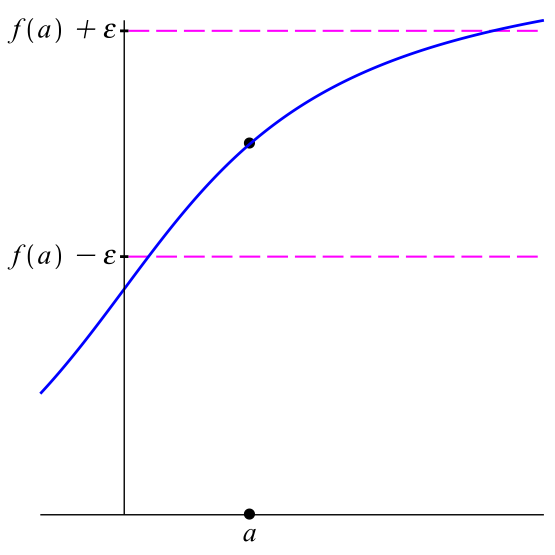
\includegraphics{Continuity_1}} \hspace{0.75in} \resizebox{!}{2.0in}{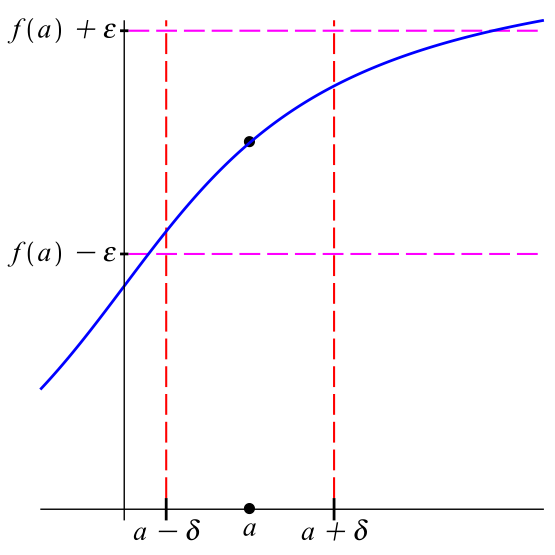
\includegraphics{Continuity_2}}
\caption{Demonstrating the definition of continuity at a point.}
\label{F:Continuity}
\end{center}
\end{figure}
Let's deal with the first statement, making the values of $f(x)$ ``as close to $f(a)$ as we want". What this means is that if we set any tolerance, say $0.0001$, then we can make the values of $f(x)$ within $0.0001$ of $f(a)$. Since the absolute value $| f(x)-f(a) |$ measures how close $f(x)$ is to $f(a)$, we can rewrite the statement that the values of $f(x)$ are within $0.0001$ of $f(a)$ as $| f(x) - f(a) | < 0.0001$. Of course, $0.0001$ may not be as close as we want to $f(a)$, so we need a way to indicate that we can make the values of $f(x)$ arbitrarily close to $f(a)$ -- within any tolerance at all. We do this by making the tolerance a parameter, $\epsilon$. Then our job is to make the values of $f(x)$ within $\epsilon$ of $f(a)$ regardless of the size of $\epsilon$. We write this as 
\[| f(x) - f(a) | < \epsilon.\]
We can picture this as shown at left in Figure \ref{F:Continuity}. Here we want to make the values of $f(x)$ lie within an $\epsilon$ band of $f(a)$ above and below $f(a)$. That is, we want to be able to make the values of $f(x)$ lie between $f(a)-\epsilon$ and $f(a)+\epsilon$. 

Now we have to address the question of how we ``make" the values of $f(x)$ to be within $\epsilon$ of $f(a)$. Since the values $f(x)$ are the dependent values, dependent on $x$, we ``make" the values of $f(x)$ have the property we want by choosing the inputs $x$ appropriately.  In order for $f$ to be continuous at $x=a$, we must be able to find $x$ values close enough to $a$ to force $| f(x) - f(a) | < \epsilon$. Pictorially, we can see how this might happen in the image at right in Figure \ref{F:Continuity}. We need to be able to find an interval around $x=a$ so that the graph of $f(x)$ lies in the $\epsilon$ band around $f(a)$ for values of $x$ in that interval. In other words, we need to be able to find some positive number $\delta$ so that if $x$ is in the interval $(a-\delta, a+\delta)$, then the graph of $f(x)$ lies in the $\epsilon$ band around $y=f(a)$. More formally, if we are given any positive tolerance $\epsilon$, we must be able to find a positive number $\delta$ so that if $| x-a | < \delta$ (that is, $x$ is in the interval $(a-\delta, a+\delta)$), then $| f(x) - f(a) | < \epsilon$ (or $f(x)$ lies in the $\epsilon$ band around $y=f(a)$).   

This gives us a rigorous definition of what it means for a function $f: \R \to \R$ to be continuous at a point.

\begin{definition} \label{def:epsilon_delta_continuity} A function $f : \R \to \R$ is \textbf{continuous at a point} $a$ if, given any $\epsilon > 0$, there exists a $\delta > 0$ so that $| x - a | < \delta$ implies $| f(x) - f(a)| < \epsilon$.
\end{definition}

Note that the value of $\delta$ can depend on the value of $a$ and on $\epsilon$, but not on values of $x$. 

\begin{pa} \label{pa:MS_continuity} The GeoGebra file at \url{https://www.geogebra.org/m/rym36sqs} will allow us to play around with this definition. Use this GeoGebra applet for the first two problems in this activity. 
\be
\item Enter $f(x)=x\sin(x)$ as your function. (You can change the viewing window coordinates, the base point $a$, and the function using the input boxes at the left on the screen.) Determine a value of $\delta$ so that $| f(x) - f(1) | < 0.5$ whenever $| x - 1 | < \delta$. Explain your method.

\item Now find a value of $\delta$ so that $| f(x) - f(2.5) | < 0.25$ whenever $| x - 2.5 | < \delta$. Explain your method.

\item ~
	\ba
	\item What is the negation of the definition of continuity at a point? In other words, what do we need to do to show that a function $f: \R \to \R$ is not continuous at a point $x=a$? 

	\item Use the negation of the definition to explain why the function $f : \R \to \R$ defined by 
	\[f(x) = \begin{cases} -1 &\text{ if } x < 1 \\ 1 &\text{ if } x \geq 1 \end{cases}\]
	is not continuous at $x=1$. 

	\ea
	
\ee


\end{pa}

\begin{comment}

\ActivitySolution
\be
\item We look for a value of $\delta$ so that the graph of $f$ on the interval $(1-\delta, 1+\delta)$ is contained entirely within the band $(f(1)-0.5, f(1)+0.5)$. A value of $\delta$ that works in this case is $\delta = 0.3$, as illustrated at left in Figure \ref{F:PA_Continuity_2}. 
 
\begin{figure}[ht]
\begin{center}
\resizebox{!}{1.8in}{\includegraphics{PAContinuity_a}} \hspace{0.5in} \resizebox{!}{1.8in}{\includegraphics{PAContinuity_b}}
\caption{Continuity at a point for Preview Activity \ref{pa:MS_continuity}.}
\label{F:PA_Continuity_2}
\end{center}
\end{figure}

\item  We look for a value of $\delta$ so that the graph of $f$ on the interval $(2.5-\delta, 2.5+\delta)$ is contained entirely within the band $(f(2.5)-0.25, f(2.5)+0.25)$. A value of $\delta$ that works in this case is $\delta = 0.1$, as illustrated at right in Figure \ref{F:PA_Continuity_2}. 

\item ~
	\ba
	\item  We negate a universal quantifier with an existential quantifier and an existential quantifier with a universal quantifier. So a function $f : \R \to \R$ is not continuous at $x=a$ if there exists an $\epsilon > 0$ so that for all $\delta > 0$, the fact that $| x-a | < \delta$ does not imply $| f(x) - f(a) | < \epsilon$. 

	\item  The graph of $f$ is shown in Figure \ref{F:PA_Continuity_3}. Let $\epsilon = 0.5$. Given $\delta > 0$, the point $x = 1-\frac{\delta}{2}$ is in the interval $(1-\delta, 1+\delta)$, but  
\[| f(x) - f(1) | = | f\left(1-\frac{\delta}{2}\right) - f(1) | = | -1 - 1 | = 2.\]
So $| f(x) - f(1) | > \epsilon$. This shows that $f$ is not continuous at $x=1$. 

\begin{figure}[ht]
\begin{center}
\resizebox{!}{2.0in}{\includegraphics{PAContinuity_c}}
\caption{The function $f$ is not continuous at $x=1$.}
\label{F:PA_Continuity_3}
\end{center}
\end{figure}

	\ea
	
\ee

\end{comment}

\csection{Continuous Functions Between Metric Spaces}\label{sec_cont_func_btwn}
In our preview activity we saw how to formally define what it means for a function $f : \R \to \R$ to be continuous at a point. 


Note that Definition \ref{def:epsilon_delta_continuity} depends only on being able to measure how close points are to each other. Since that is precisely what a metric does, we can extend this notion of continuity to define continuity for functions between metric spaces. Continuity is an important idea in topology, and we will work with this idea extensively throughout the semester.
 
If we let $d_E : \R \times \R \to \R$ be defined by $d_R(x,y) = | x - y |$, then we have seen that $d_E$ is a metric on $\R$ (note that $d_E$ is the Euclidean metric on $\R$). Using this metric we can reformulate what it means for a function $f : \R \to \R$ to be continuous at a point.

\begin{definition}[Alternate Definition] A function $f : \R \to \R$ is \textbf{continuous at a point} $a$ if, given any $\epsilon > 0$, there exists a $\delta > 0$ so that $d_E(x,a) < \delta$ implies $d_E(f(x), f(a)) < \epsilon$.
\end{definition}

This alternate definition depends on the metric $d_E$. We could easily replace the metric $d$ with any other metric we choose. This allows us to define continuity at a point for functions between metric spaces.

\begin{definition} Let $(X,d_X)$ and $(Y, d_Y)$ be metric spaces. A function $f:X \to Y$ is \textbf{continuous}\index{continuity at a point in a metric space} at $a \in X$ if, given any $\epsilon > 0$, there exists a $\delta > 0$ so that $d_X(x,a)< \delta$ implies $d_Y(f(x), f(a)) < \epsilon$.  
\end{definition}

Once we have defined continuity at a point, we can define continuous functions.

\begin{definition} Let $(X,d_X)$ and $(Y, d_Y)$ be metric spaces. A function $f:X \to Y$ is \textbf{continuous}\index{continuous function} if $f$ is continuous at every point in $X$. 
\end{definition}

\begin{example} In general, to prove that a function $f:X \to Y$ is continuous, where $(X,d_X)$ and $(Y, d_Y)$ are metric spaces, we begin by choosing an arbitrary element $a$ in $X$. Then we let $\epsilon$ be a number greater than $0$ and show that there is a $\delta > 0$ so that $d_Y(f(x),f(a)) < \epsilon$ whenever $d_X(x,a) < \delta$. The $\delta$ we need cannot depend on $x$ (since $x$ isn't known), but can depend on the value of $a$ that we choose, and will likely depend on $\epsilon$ as well. That is, there is a function $C$ of only the independent variables $a$ and $\epsilon$ that produces the $\delta$, or $\delta = C(a,\epsilon)$. As an example, let $X = \R$ and let $d_X$ be defined as 
\[d_X(x,y) = \min\{|x-y|,1\}.\]
The proof that $d_X$ is a metric is left for Exercise \ref{ex:min_1_metric}. Consider $f : X \to Y$ defined by $f(x) = x^2$, where $(Y,d_Y) = (\R, d_E)$. To show that $f$ is continuous, we let $a \in \R$ and let $\epsilon > 0$. 

\begin{quote} \textbf{Scratch work.} What happens next is not part of the proof, but shows how we go about finding a $\delta$ we need. We are looking for $\delta > 0$ such that $d_X(x,a) < \delta$ implies that $d_E(f(x),f(a)) < \epsilon$. That is, we want to make 
\[d_E(f(x),f(a)) = \sqrt{(f(x)-f(a))^2} = |f(x)-f(a)| = |x^2-a^2| < \epsilon\]
whenever
\[d_X(x,a) = \min\{|x-a|, 1\} < \delta.\]
Now $|x^2-a^2| = |(x-a)(x+a)| = |x-a| \ |x+a|$. If $d_X(x,a) < \delta$, then $\min\{|x-a|, 1\} < \delta$. If we choose $\delta < 1$, then $d_X(x,a) < \delta < 1$ implies that $|x-a| < 1$ and so $d_X(x,a) = |x-a|$. Now
\[|x+a| = |(x-a) + 2a| \leq |x-a| + 2|a| < 1+2|a|.\]
It follows that 
\[|x-a| \ |x+a| < \delta(1+2|a|).\]
To make this product less that $\epsilon$, we can choose $\delta$ such that $\delta(1+2|a|) < \epsilon$ or $\delta < \frac{\epsilon}{1+2|a|}$. That is, there is a function $C$ of $\epsilon$ that gives us the $\delta$ we want, namely $\delta = C(a,\epsilon) = \left\{1, \frac{\epsilon}{1+2|a|}\right\}$. 

Now we ignore this paragraph and present the proof, which is essentially reversing the steps we just made. If the steps can't be reversed, then we have to rethink our argument. The next step in the proof might seem like magic to the uninitiated reader, but we have seen behind the curtain so it isn't a mystery to us.
\end{quote}

\noindent Let $\delta$ be a positive number less than $\min\left\{1, \frac{\epsilon}{1+2|a|}\right\}$. Then 
\[d_X(x,a) = \min\{|x-a|,1\} < \delta\]
implies that $d_X(x,a) < \delta < 1$ and so $d_X(x,a) = |x-a| < \delta < 1$. Then
\[|x+a| = |(x-a) + 2a| \leq |x-a| + 2|a| < 1+2|a|.\]
It follows that
\begin{align*}
d_E(f(x),f(a)) &= \sqrt{(f(x)-f(a))^2} \\
	&= |f(x)-f(a)| \\
	&= |x^2-a^2| \\
	&= |(x-a)(x+a)| \\
	&= |x-a| \ |x+a| \\
	&< \delta (1+2|a|) \\
	&<  \left(\frac{\epsilon}{1+2|a|}\right) (1+2|a|) \\
	&= \epsilon.
\end{align*}
We conclude that $f$ is continuous at every point in $X$ and so $f$ is a continuous function.
\end{example}

Not all functions are continuous as we see in the next example. 

\begin{example} \label{exp:not_continuous} Let $X = Y = \R$ and define $f : X \to Y$  by $f(x) = x$. Let $d_X$ be the Euclidean metric and $d_Y$ the discrete metric. (Recall that $d_Y(x,y) = 1$ whenever $x \neq y$.) Let $a \in X$ and let $0 < \epsilon < 1$. 
 
Let $\delta > 0$, and let $x = a+\frac{\delta}{2}$. Then $x \neq a$ and $d_X(x,a) < \delta$. However, 
\[d_Y(f(x),f(a)) = d_Y(x,a) = 1.\]
So if $0 < \epsilon < 1$, there is no $\delta > 0$ such that $d_X(x,a) < \delta$ implies that $d_Y(f(x),f(a)) < \epsilon$. We conclude that $f$ is continuous at no point in $X$.  
\end{example}

Certain functions are always continuous, as the next activity shows.

\begin{activity} \label{act:id_constant_continuous} ~ 
	\ba
	\item Let $(X, d_X)$ and $(Y, d_Y)$ be metric spaces, and let $b \in Y$. Define $f : X \to Y$ by $f(x) = b$ for every $x \in X$. Show that $f$ is a continuous function.
		
	\item Let $(X, d)$ be a metric space. Define the function $i_X : X \to X$ by $i_X(x) = x$ for every $x \in X$. Show that $i_X$ is a continuous function. (The function $i_X$ is called the \emph{identity function}\index{identity function} on $X$.)
	
	\item Why doesn't the argument in part (b) contradict Example \ref{exp:not_continuous}?
		
	\ea
\end{activity}

\begin{comment}

\ActivitySolution
	\ba
	\item Let $a \in X$ and let $\epsilon$ be greater than 0. Choose $\delta$ to be any positive number. If $d_X(x,a) < \delta$, then $d_Y(f(x),f(a)) = d_Y(b,b) = 0 < \epsilon$.  Therefore, $f$ is continuous at every point in $X$ and so is a continuous function. 
		
	\item Let $a \in X$ and let $\epsilon$ be greater than 0. Choose $\delta = \epsilon$. If $d_X(x,a) < \delta$, then $d_X(f(x),f(a)) = d_X(x,a) < \delta = \epsilon$.  Therefore, $f$ is continuous at every point in $X$ and so is a continuous function. 
	
	\item In Example \ref{exp:not_continuous} the domain and codomain are different metric spaces, which is not the case in (b).	
	\ea

\end{comment}

More complicated examples are in the next activity.

\begin{activity} Let $X = (\R^2, d_T)$ and $Y = (\R^2, d_M)$, where 
\[d_T((x_1, x_2), (y_1,y_2)) = | x_1-y_1 | + | x_2-y_2 |\]
is the taxicab metric and 
\[d_M((x_1, x_2), (y_1,y_2)) = \max\{| x_1-y_1 |,  | x_2-y_2 |\}\]
is the max metric. Define $f : \R^2 \to \R^2$ by $f((a,b)) = (a+b, b)$.
	\ba
	\item Is $f$ a continuous function from $X$ to $Y$? Justify your answer.
	
	\item Is $f$ a continuous function from $Y$ to $X$? Justify your answer.
	
	
	\ea
\end{activity}

\begin{comment}

\ActivitySolution

	\ba
	\item  Let $a=(a_1,a_2) \in \R^2$ and let $\epsilon > 0$. Choose any $0 < \delta < \epsilon$. Let $x = (x_1,x_2)$ in $\R^2$ and suppose $d_T(x,a) < \delta$. Then
\[d_T(x,a) = | x_1-a_1\ | + | x_2-a_2 | < \delta = \epsilon.\]
It follows that
\begin{align*}
d_M(f(x), f(a)) &= d_M((x_1+x_2, x_1), (a_1+a_2, a_2)) \\
	&= \max\{ | (x_1+x_2)-(a_1+a_2) |, | x_2-a_2 | \} \\
	&= \max\{ | (x_1-a_1)+(x_2-a_2) |, | x_2-a_2 | \} \\
	&\leq \max\{ | x_1-a_1 | + | x_2-a_2 |, | x_2-a_2 | \} \\
	&= |x_1-a_1|+|x_2-a_2| < \epsilon.
	\end{align*}
Thus, the function $f$ is continuous at every point in $\R^2$ and is therefore a continuous function from $X$ to $Y$. 

	\item  Let $a=(a_1,a_2) \in \R^2$ and let $\epsilon > 0$. Choose any $0 < \delta < \frac{\epsilon}{3}$. Let $x = (x_1,x_2)$ in $\R^2$ and suppose $d_M(x,a) < \delta$. Then
\[d_M(x,a) = \max\{| x_1-a_1\ |, | x_2-a_2 |\} < \delta < \frac{\epsilon}{3}.\]
So $| x_1-a_1 | < \frac{\epsilon}{3}$ and $| x_2-a_2 | < \frac{\epsilon}{3}$. Then
\begin{align*}
d_T(f(x), f(a)) &= d_T((x_1+x_2, x_1), (a_1+a_2, a_2)) \\
	&= | (x_1+x_2)-(a_1+a_2) | + | x_2-a_2 |  \\
	&= | (x_1-a_1)+(x_2-a_2) | + | x_2-a_2 | \} \\
	&\leq \left(| x_1-a_1 | + | x_2-a_2 |\right) + | x_2-a_2 | \\
	&\leq \frac{\epsilon}{3}+\frac{\epsilon}{3} + \frac{\epsilon}{3}  \\
	&= \epsilon.
\end{align*}
Thus, the function $f$ is continuous at every point in $\R^2$ and is therefore a continuous function from $Y$ to $X$. 
	
	\ea

\end{comment}

\csection{Composites of Continuous Functions}\label{sec_comp_cont_func}

Let $(X, d_X)$, $(Y,d_Y)$, and $(Z, d_Z)$ be metric spaces, and suppose $f: X \to Y$ and $g: Y \to Z$ are continuous functions. It seems natural to ask if the composite $g \circ f : X \to Z$ is a continuous function.

\begin{activity}  Let $(X, d_X)$, $(Y,d_Y)$, and $(Z, d_Z)$ be metric spaces, and suppose $f: X \to Y$ and $g: Y \to Z$ are continuous functions. We will prove that $g \circ f$ is a continuous function. 
	\ba
	\item What do we have to do to show that $g \circ f$ is a continuous function? What are the first two steps in our proof?
		
	\item Let $a \in X$ and let $b = f(a)$. Suppose $\epsilon > 0$ is given. Explain why there must exist a $\delta_1 > 0$ so that $d_Y(y,b) < \delta_1$ implies $d_Z(g(y), g(b)) < \epsilon$. 
		
	\item Now explain why there exists a $\delta_2 > 0$ so that $d_X(x,a) < \delta_2$ implies that $d_Y(f(x), f(a)) < \delta_1$. 
		
	\item Prove that $g \circ f : X \to Z$ is a continuous function.
			
	\ea
\end{activity}

\begin{comment}

\ActivitySolution
	\ba
	\item We have to start with a point $a \in X$ and an $\epsilon$ greater than $0$. We have to find a positive number $\delta$ such that $d_X(x,a) < \delta$ implies that $d_Z((g \circ f)(x), (g \circ f)(a)) < \epsilon$. 
		
	\item Since $g$ is continuous at $b$, there exists a $\delta_1 > 0$ so that $d_Y(y,b)  < \delta_1$ implies $d_Z(g(y), g(b)) < \epsilon$. 
		
	\item Since $f$ is continuous at $a$, there exists a $\delta_2 > 0$ so that $d_X(x,a) < \delta_2$ implies that $d_Y(f(x), f(a)) < \delta_1$ (here we are using $\delta_1$ as our $\epsilon$). 
		
	\item Let $\delta = \delta_2$ and suppose that $d_X(x,a) < \delta$. Then $d_Y(f(x),f(a)) < \delta_1$. But then $d_Z(g(f(x)), g(f(a)) < \epsilon$. This shows that $g \circ f : X \to Z$ is a continuous function.
			
	\ea

\end{comment}


Continuity is an important concept in topology. We have seen how to define continuity in metric spaces, and we will soon expand on this idea to define continuity without reference to metrics at all. This will allow us to later define continuous functions between arbitrary topological spaces. 


\csection{Summary}\label{sec_cont_func_summ}
Important ideas that we discussed in this section include the following.
\begin{itemize}
\item Let $(X,d_X)$ and $(Y, d_Y)$ be metric spaces. A function $f:X \to Y$ is continuous at $a \in X$ if, given any $\epsilon > 0$, there exists a $\delta > 0$ so that $d_X(x,a)< \delta$ implies $d_Y(f(x), f(a)) < \epsilon$.  

\item Let $(X,d_X)$ and $(Y, d_Y)$ be metric spaces. A function $f:X \to Y$ is continuous if $f$ is continuous at every point in $X$.
\end{itemize}

\csection{Exercises}\label{sec_cont_func_exer}

\be

\item Let $f: \R \to \R$ be defined by $f(x) = |x|$, with the Euclidean metric on both the domain and the codomain. Is $f$ continuous at $x=0$? Prove your answer.

\begin{comment}

\ExerciseSolution The answer is yes. Let $\epsilon$ be greater than $0$. Let $\delta = \epsilon$. Then $|x - 0| < \delta$ means that $|x| < \delta$. Then $|f(x)-f(0)| = |x| < \delta = \epsilon$. So $f$ is continuous at $0$. 

\end{comment}

\item Let $f: \R \to \R$ be defined by $f(x) = \begin{cases} \frac{x}{|x|} &\text{ if } x \neq 0 \\ 1 &\text{ if } x=0. \end{cases}$ Is $f$ continuous at $x=0$? Prove your answer.

\begin{comment}

\ExerciseSolution The answer is no. Let $\epsilon$ be greater than $0$ and less than $1$, and let $\delta$ be greater than $0$. If $x \in (0, \delta)$, then $f(x) = 1$. Then $|x - 0| < \delta$ implies that 
\[|f(x)-f(0)| = |1-0|  = 1 > \epsilon.\]   


\end{comment}


\item Let $(Y, d_Y) = (\R, d_E)$, where $d_E$ is the Euclidean metric. %On $\R$ we have $d_E(a,b) = |a-b|$. 
\ba
\item Let $(X,d_X) = (\R^2, d_E)$.  Prove or disprove: the function $f:X \to Y$ defined by $f((x_1,x_2)) = x_1 + x_2$ is continuous. 

\item Let $(X,d_X) = (\R^2, d_M)$ where $d_M$ is the max metric.  Prove or disprove: the function $f:X \to Y$ defined by $f((x_1,x_2)) = x_1 + x_2$ is continuous. 

\ea


\begin{comment}

\ExerciseSolution 
\ba
\item Let $a = (a_1, a_2)$ be in $X$.  We will demonstrate that $f$ is continuous at $a$.  Let $\epsilon$ be greater than $0$. Let $\delta = \frac{\epsilon}{2}$. Suppose $x = (x_1,x_2) \in X$ such that $d_E(x,a) < \delta$. Then
\[d_E(x,a) = \sqrt{(x_1-a_1)^2 + (x_2-a_2)^2} < \delta.\]
Now
\[|x_1-a_1| = \sqrt{(x_1-a_1)^2} \leq \sqrt{(x_1-a_1)^2 + (x_2-a_2)^2} < \delta = \frac{\epsilon}{2}\]
and
\[|x_2-a_2| = \sqrt{(x_2-a_2)^2} \leq \sqrt{(x_1-a_1)^2 + (x_2-a_2)^2} < \delta = \frac{\epsilon}{2}.\]
This implies that 
\begin{align*}
d_E(f(x),f(a)) &= |(x_1+x_2)-(a_1+a_2)| \\
	&= |(x_1-a_1)+(x_2-a_2)| \\
	&\leq |x_1-a_1| + |x_2-a_2| \\
	&< \frac{\epsilon}{2} + \frac{\epsilon}{2} \\
	&= \epsilon.
\end{align*}
Thus, $f$ is continuous at every point in $X$ and so $f$ is a continuous function.

\item Let $a = (a_1, a_2)$ be in $X$.  We will demonstrate that $f$ is continuous at $a$.  Let $\epsilon$ be greater than $0$. Let $\delta = \frac{\epsilon}{2}$. Suppose $x = (x_1,x_2) \in X$ such that $d_M(x,a) < \delta$. Then
\[d_M(x,a) = \max\{|x_1-a_1|, |x_2-a_2|\}  < \delta = \epsilon.\]
\begin{align*}
d_E(f(x),f(a)) &= |(x_1+x_2)-(a_1+a_2)| \\
	&= |(x_1-a_1)+(x_2-a_2)| \\
	&\leq |x_1-a_1| + |x_2-a_2| \\
	&< \frac{\epsilon}{2} + \frac{\epsilon}{2} \\
	&= \epsilon.
\end{align*}
Thus, $f$ is continuous at every point in $X$ and so $f$ is a continuous function.


\ea

\end{comment} 


\item Let $X$ be any set and define $d : X \times X \to \R$ by 
\[d(x,y) = \begin{cases} 0 &\text{ if } x=y \\ 1 &\text{ if } x \neq y. \end{cases}\]
Exercise \ref{ex:MS_discrete} on page \pageref{ex:MS_discrete} asks us to show that $d$ is a metric (the discrete metric) on $\R$. 

Let $(X,d_X)$ and $(Y, d_Y)$ be metric spaces with $d_X$ the discrete metric. Determine all of the continuous functions $f$ from $X$ to $Y$. 

\begin{comment}

\ExerciseSolution We will prove that any function $f: X \to Y$ is continuous. Let $f: X \to Y$ be a function and let $a \in X$. Let $\epsilon$ be a positive real number and let $\delta = 1$. For any $x \in X$ with $d_X(x,a) < \delta$, it must be the case that $x = a$. It follows that $d_Y(f(x),f(a)) = d_Y(f(a),f(a)) = 0 < \epsilon$. So $f$ is continuous at every point in $X$ and $f$ is a continuous function.  

\end{comment}

\item \label{ex:sum_continuous} Let $f$ and $g$ be continuous functions from $(\R,d_E)$ to $(\R, d_E)$. 
	\ba
	\item Let $k \in \R$ with $k \neq 0$ and define $kf : \R \to \R$ by $(kf)(x) = kf(x)$ for all $x \in \R$. Show that $kf$ is a continuous function.
	
	
	\item Define $f+g : \R \to \R$ by $(f+g)(x) = f(x) + g(x)$ for all $x \in \R$. Show that $f+g$ is a continuous function.
	
	\ea
	
\begin{comment}

\ExerciseSolution

\ba

\item Let $\epsilon > 0$ be given and let $a \in \R$. Since $f$ is continuous at $a$ there is a $\delta > 0$ such that $d_E(f(x),f(a)) < \frac{\epsilon}{|k|}$ whenever $d_E(x,a) < \delta$. Then
\[d_E((kf)(x), (kf)(a)) = d_E(kf(x), kf(a)) = |kf(x)-kf(a)| = |k||f(x)-f(a)| < |k|\ \frac{\epsilon}{k} = \epsilon\]
whenever $d_E(x,a) < \delta$. We conclude that $kf$ is continuous at every $a \in \R$ and so $kf$ is a continuous function. 


\item Let $\epsilon$ be greater than $0$ and let $a \in \R$. Since $f$ is continuous at $a$, there exists $\delta_f > 0$ such that $d_E(f(x),f(a)) < \frac{\epsilon}{2}$ whenever $d_E(x,a) < \delta_f$. Similarly, since $g$ is continuous at $a$, there exists $\delta_g > 0$ such that $d_E(g(x),g(a)) < \frac{\epsilon}{2}$ whenever $d_E(x, a) < \delta_g$. Let $\delta = \min\left\{\delta_f, \delta_g\right\}$. Now suppose that $d_E(x,a) < \delta$. Then 
\begin{align*}
d_E((f+g)(x), (f+g)(a)) &= d_E(f(x)+g(x), f(a) + g(a)) \\
	&= |f(x)-f(a) + g(x)-g(a)| \\
	&\leq |f(x)-f(a)| + |g(x)-g(a)| \\
	&= d_E(f(x),f(a)) + d_E(g(x), g(a)) \\
	< \frac{\epsilon}{2} + \frac{\epsilon}{2} \\
	&= \epsilon.
\end{align*}
Thus, $f+g$ is a continuous function.

\end{comment}

\item Let $f$ and $g$ be continuous functions from $(\R, d_E)$ to $(\R,d_E)$. In this exercise we will prove that $fg$ is a continuous function from $\R$ to $\R$.  Let $a$ be in $\R$, and follow the steps below to show that $fg$ is continuous at $x=a$. Let $\epsilon$ be a positive number.

	\ba
	
	\item We will first want to express $f(x)g(x) - f(a)g(a)$ in a more useful way. Use the fact that $f(x) = f(a) + (f(x)-f(a))$ and $g(x)  = g(a) + (g(x)-g(a))$ to show that 
	\begin{equation*}
	f(x)g(x)-f(a)g(a) = f(a)(g(x)-g(a)) + g(a)(f(x)-f(a)) + (f(x)-f(a))(g(x)-g(a)).
	\end{equation*}
	
	\item Explain why there exist positive numbers $\delta_1$, $\delta_2$, $\delta_3$, and $\delta_4$ such that 
\begin{align*}
|f(x)-f(a)| < \sqrt{\frac{\epsilon}{3}} &\text{ when } |x-a| < \delta_1 \\
|g(x)-g(a)| <  \sqrt{\frac{\epsilon}{3}}  &\text{ when } |x-a| < \delta_2 \\
|f(x)-f(a)| < \frac{\epsilon}{3(1+|g(a)|)}  &\text{ when } |x-a| < \delta_3 \\
|g(x)-g(a)| < \frac{\epsilon}{3(1+|f(a)|)}  &\text{ when } |x-a| < \delta_4.
\end{align*}

	\item Use the results of (a) and (b) to show that $fg$ is continuous at $x=a$. (Hint: $1+|f(a)| > |f(a)|$.)

	
	
	\ea
	
\begin{comment}

\ExerciseSolution

\ba

\item We write $f(x)$ and $g(x)$ as $f(x) = f(a) + (f(x)-f(a))$ and $g(x)  = g(a) + (g(x)-g(a))$. Then
\begin{align*}
f(x)g(x)-f(a)g(a) &= \big(f(a) + (f(x)-f(a))\big) \big(g(a) + (g(x)-g(a)) \big) - f(a) g(a) \\
	&= f(a)(g(x)-g(a)) + g(a)(f(x)-f(a)) + (f(x)-f(a))(g(x)-g(a)).
\end{align*}

\item Since $\sqrt{\frac{\epsilon}{3}}$ is a positive number and since $f$ is continuous at $x=a$, there exists a positive number $\delta_1$ such that 
\[|f(x)-f(a)| < \sqrt{\frac{\epsilon}{3}} \text{ when } |x-a| < \delta_1.\]
A similar argument shows that 
\begin{align*}
|g(x)-g(a)| <  \sqrt{\frac{\epsilon}{3}}  &\text{ when } |x-a| < \delta_2 \\
|f(x)-f(a)| < \frac{\epsilon}{3(1+|g(a)|)}  &\text{ when } |x-a| < \delta_3 \\
|g(x)-g(a)| < \frac{\epsilon}{3(1+|f(a)|)}  &\text{ when } |x-a| < \delta_4
\end{align*}
for some positive real numbers $\delta_2$, $\delta_3$, and $\delta_4$. 

\item Now let $\delta$ be the minimum of $\delta_1$, $\delta_2$, $\delta_3$, and $\delta_4$. It follows that 
\begin{align*}
|f(x)g(x)-f(a)g(a)| &= \left|\big(f(a) + (f(x)-f(a))\big) \big(g(a) + (g(x)-g(a)) \big) - f(a) g(a) \right| \\
	&= |f(a)(g(x)-g(a)) + g(a)(f(x)-f(a)) + (f(x)-f(a))(g(x)-g(a))| \\ 
	&\leq |f(a)| \ |g(x)-g(a)| + |g(a)| \ |f(x)-f(a)| + |f(x)-f(a)| \ |g(x)-g(a)| \\
	&< (1+|f(a)|) \left(\frac{\epsilon}{3(1+|f(a)|)}  \right) + (1+|g(a)|) \left( \frac{\epsilon}{3(1+|g(a)|)}  \right) + \left(\sqrt{\frac{\epsilon}{3}}\right) \left(\sqrt{\frac{\epsilon}{3}}\right) \\
	&= \frac{\epsilon}{3} + \frac{\epsilon}{3}  + \frac{\epsilon}{3}  \\
	&= \epsilon.
\end{align*}
So $fg$ is a continuous function. 

\ea

\end{comment}
	
\item Let $f$ and $g$ be functions from $(\R,d_E)$ to $(\R,d_E)$. 

\ba

\item Is it true that if $f+g$ is a continuous function, then $f$ and $g$ are continuous functions? Verify your answer.

\item Is it true that if $fg$ is a continuous function, then $f$ and $g$ are continuous functions? Verify your answer. 

\ea

\begin{comment}

\ExerciseSolution

\ba

\item The answer is no. Let $f: \R \to \R$ with the Euclidean metric on both the domain and codomain be defined by $f(x) = \begin{cases} 1 &\text{ if } x \geq 0 \\ 0 &\text{ if } x < 0. \end{cases}$. Let $g(x) = -f(x)$ for all $x \in \R$. Then $f+g$ is the constant function $0$ and so $f+g$ is a continuous function. However, the function $f$ is not continuous at $x=0$. To see why, let $\epsilon = \frac{1}{2}$. For any $\delta > 0$, if $x \in (0, \delta)$, then $f(x) = 1$. So $|x - 0| < \delta$ does not imply that $|f(x)-f(0)| < \epsilon$.   

\item Again, the answer is no. Let $f(x)$ be as in part (a) and let $g(x) = \begin{cases} 0 &\text{ if } x \geq 0 \\ 0 &\text{ if } x < 1. \end{cases}$. Then $fg$ is the constant function $0$ but $f$ is not continuous at $x=0$.

\ea


\end{comment}


\item Let $f(x) = 2x^2+1$ map from $\R$ to $\R$, with both the domain and codomain having the Euclidean metric.

	\ba
	
	\item Let $\epsilon = \frac{1}{4}$. Find a value of $\delta$ such that $|x-1| < \delta$ implies that $|f(x)-f(a)| < \epsilon$. You might use the applet at  to confirm your value of $\delta$. 
	
	\item Prove that $f$ is continuous at $x=1$. 
	
	\ea
	
\begin{comment}

\ExerciseSolution

\ba

\item First we find a candidate for our value for $\delta$, then we show that our value of $\delta$ works. To find a value of $\delta$, we work backwards. Note that $|x - 1| < \frac{1}{4}$ implies that $-\frac{1}{4} < x-1 < \frac{1}{4}$ or that $\frac{7}{4} < x+1 < \frac{9}{4}$. Thus, $\frac{7}{4} < |x+1| < \frac{9}{4}$ and $\frac{4}{9} < \frac{1}{|x+1|} < \frac{4}{7}$. Assume $|f(x)-f(a)| < \frac{1}{4}$. Then
\begin{align*}
| 2x^2+1 - (2(1)^2+1)| &< \frac{1}{4} \\
|2x^2-2| &< \frac{1}{4} \\
|x^2-1| &< \frac{1}{8} \\
|x-1||x+1| &< \frac{1}{8} \\
|x-1| &< \frac{1}{8}\left(\frac{1}{|x+1|}\right). 
\end{align*}
So if we choose $\delta = \frac{1}{8}\left(\frac{4}{9}\right)$, then 
\[|x-1| < \delta < \frac{1}{8}\left(\frac{4}{9}\right) < \frac{1}{8}\left(\frac{1}{|x+1|}\right).\] 

Now we reverse the process to show that this value of $\delta$ works. Let $\delta = \frac{1}{18} = \frac{1}{8}\left(\frac{4}{9}\right)$. Then $|x -1 | < \delta$ implies 
\begin{align*}
|x-1| &< \frac{1}{8}\left(\frac{4}{9}\right) \\
|x-1| &< \frac{1}{8}\left(\frac{1}{|x+1|}\right) \\
|x-1||x+1| &< \frac{1}{8} \\
|x^2-1| &< \frac{1}{8} \\
|2x^2-2| &< \frac{1}{4} \\
| 2x^2+1 - (2(1)^2+1)| &< \frac{1}{4} \\
|f(x) - f(1)| &< \epsilon.
\end{align*}

\item In (a) we showed that if $\epsilon$ is greater than or equal to $\frac{1}{4}$, we can find a $\delta$ such that $|x-1| < \delta$ implies $|f(x)-f(a)| < \epsilon$. So let $\epsilon > 0$ and $\$\epsilon < \frac{1}{4}$. Then $|x - 1| < \epsilon$ implies that $-\epsilon < x-1 < \epsilon$ or that $2-\epsilon < x+1 < 2+\epsilon$. Thus, $\frac{1}{2+\epsilon} < |x+1| < \frac{1}{2-\epsilon}$. To find the $\delta$ we want, assume $|f(x)-f(a)| < \epsilon$. Then
\begin{align*}
| 2x^2+1 - (2(1)^2+1)| &< \epsilon \\
|2x^2-2| &< \epsilon \\
|x^2-1| &< \frac{\epsilon}{2} \\
|x-1||x+1| &< \frac{\epsilon}{2} \\
|x-1| &< \frac{\epsilon}{2}\left(\frac{1}{|x+1|}\right).
\end{align*}
To make $|x-1| < \frac{\epsilon}{2}\left(\frac{1}{|x+1|}\right)$ we can use $\delta = \frac{\epsilon}{2}\left(\frac{1}{2+\epsilon}\right)$.

Let $\delta = \frac{\epsilon}{2}\left(\frac{1}{2+\epsilon}\right)$. Then $|x -1 | < \delta$ implies 
\begin{align*}
|x-1| &< \frac{\epsilon}{2}\left(\frac{1}{2+\epsilon}\right)\\
|x-1| &< \frac{\epsilon}{2}\left(\frac{1}{|x+1|}\right) \\
|x-1||x+1| &< \frac{\epsilon}{2}  \\
|x^2-1| &< \frac{\epsilon}{2} \\
|2x^2-2| &< \epsilon \\
| 2x^2+1 - (2(1)^2+1)| &< \epsilon  \\
|f(x) - f(1)| &< \epsilon.
\end{align*}
Therefore, $f$ is continuous at $x=1$. 


\ea

\end{comment}

%\item Let $(X, d_X)$, $(Y, d_Y)$, and $(Z, d_Z)$ be metric spaces, and let $f: X \to Y$ and $g: Y \to Z$ be continuous functions. Prove that $(g \circ f)$ is a continuous function from $X$ to $Z$. 

%\begin{comment}

%\ExerciseSolution Let $a \in X$. Let $\epsilon$ be a positive number. Let $y = f(x)$ and let $b = f(a)$. The fact that $g$ is a continuous function means that $g$ is continuous at $b$. So there exists a positive real number $\delta'$ such that $d_Z(g(y), g(b)) < \epsilon$ whenever $d_Y(y,b) < \delta'$. Since $f$ is continuous at $x=a$, there is a positive number $\delta$ such that $d_Y(f(x),f(a)) < \delta'$ whenever $d_X(x, a) < \delta$. So when $d_X(x, a) < \delta$, we have $d_Y(f(x), f(a)) = d_Y(y, b) < \delta'$ and 
%\begin{align*}
%d_Z((g \circ f)(x), (g \circ f)(a)) &= d_Z(g(f(x)), g(f(a))) \\
%	&=d_Z(g(y), g(b)) \\
%	&< \epsilon.
%\end{align*}
 
%\end{comment}




\item \label{ex:min_1_metric} Define $d: \R \times \R \to \R$ as 
\[d(x,y) = \min\{|x-y|,1\}.\]
Prove that $d$ is a metric.

\begin{comment}

\ExerciseSolution Let $x, y, z \in \R$. By definition, $d(x,y) \geq 0$. Since $|x - x| = 0$, we see that $d(x,x) = 0$. Also, if $d(x,y) = 0$, then $0 = d(x,y) = |x-y|$ and $x=y$. 

If $d(x,y) = 1$, then $|x-y| = |y-x| \geq 1$ and so $d(y,x) = d(x,y) = 1$. If $d(x,y) < 1$, then $|x-y| = |y-x| < 1$ and so $d(y,x) = |y-x| = d(x,y)$. 

Finally, we verify the triangle inequality using cases.
\begin{itemize}
	\item Suppose one of $d(x,y)$ is $1$. Without loss of generality, assume $d(x,y) = 1$. Now $d(x,z) \leq 1$, so 
\[d(x,z) \leq 1 \leq 1 + d(y,z) = d(x,y) + d(y,z).\]

\item Suppose that $d(x,y) = |x-y| < 1$ and $d(y,z) = |y-z| < 1$. Since $d(x,z) \leq |x-z|$ we have 
\[d(x,z) \leq |x-z| \leq |x-y|+|y-z| = d(x,y) + d(y,z).\]	
	
	\end{itemize}
	
\end{itemize}

We conclude that $d$ is a metric on $\R$. 

\end{comment}


\item Let $f : \R \to \R$ be a continuous function, with both copies of $\R$ having the Euclidean metric. Assume that $f(x) = 0$ whenever $x$ is rational. Prove that $f(x) = 0$ for every $x \in \R$. (Hint: Use Exercise \ref{ex:GLB_rational} on page \pageref{ex:GLB_rational}.)

\begin{comment}

\ExerciseSolution Suppose to the contrary that $f(y) \neq 0$ for some irrational number $y$. Let $\epsilon$ be a positive real number less than $|f(y)|$. Let $\delta$ be a positive real number. By Exercise \ref{ex:GLB_rational} on page \pageref{ex:GLB_rational} we can always find a rational number between any two real numbers. So there is a rational number $r$ in the interval $(y - \delta, y + \delta)$. So even though $|r - y| < \delta$, we have $|f(r)-f(y)| = |f(y)| > \epsilon$. This implies that $f$ is not continuous at $y$, a contradiction. We conclude that $f(y) = 0$ for every irrational number $y$ and $f(x) = 0$ for every $x \in \R$. 

\end{comment}

\item Let $f: \R \to \R$ be defined by $f(x) = 0$ if $x$ is irrational and $f(x) = 1$ if $x$ is rational. Assume the Euclidean metric on both copies of $\R$. Show that $f$ is not continuous at any point in $\R$. (Hint: Use Exercise \ref{ex:GLB_rational} on page \pageref{ex:GLB_rational} and Exercise \ref{ex:GLB_irrational} on page \pageref{ex:GLB_irrational}.)


\begin{comment}

\ExerciseSolution Let $a \in \R$. We first show that $f$ is not continuous at $a$ if $a$ is rational. Let $\epsilon$ be a positive real number less than $1$. Let $\delta$ be a positive real number. By Exercise \ref{ex:GLB_irrational} on page \pageref{ex:GLB_irrational}, we can always find an irrational number between any two real numbers. So there is an irrational number $z$ in the interval $(a - \delta, a + \delta)$. So even though $|z - a| < \delta$, we have $|f(z)-f(a)| = |f(a)| > \epsilon$. This implies that $f$ is not continuous at $a$. 

Now assume that $a$ is an irrational number. Let $\epsilon$ be a positive real number less than $1$. Let $\delta$ be a positive real number. By Exercise \ref{ex:GLB_rational} on page \pageref{ex:GLB_rational}, we can always find a rational number between any two real numbers. So there is a rational number $r$ in the interval $(a - \delta, a + \delta)$. So even though $|r - a| < \delta$, we have $|f(r)-f(a)| = |f(r)| > \epsilon$. This implies that $f$ is not continuous at $a$. So $f$ is not continuous at any real number.

\end{comment}


\item Let $g: \R \to \R$ be defined by $g(x) = 0$ if $x$ is irrational and $g(x) = x$ if $x$ is rational. Assume the Euclidean metric on both copies of $\R$. Show that $g$ is continuous only at $0$. 

\begin{comment}

\ExerciseSolution First we demonstrate that $g$ is continuous at $0$. Let $\epsilon$ be a positive real number and let $\delta = \epsilon$. Suppose $x \in \R$ with $|x - 0| = |x| < \delta$. If $x$ is irrational then 
\[|g(x)-g(0)| = |g(x)| = 0 < \epsilon\]
and if $x$ is rational then 
\[|g(x)-g(0)| = |g(x)| = |x| < \delta = \epsilon.\]
Therefore, $g$ is continuous at $0$. 

Now suppose $a \neq 0$. Let $\epsilon < |a|$ and $\delta$ be positive. We consider cases.
\begin{description}
\item[$a$ is irrational:] Let $x$ be a rational number in $(a-\delta, a+\delta)$ with $|x| > |a|$. Then $|x - a| < \delta$ but 
\[|g(x)-g(a)| = |g(x)| = |x| > |a| > \epsilon.\]
So $g$ is not continuous at $a$.
\item[$a$ is rational:] Let $x$ be an irrational number in $(a-\delta, a+\delta)$ with $|x| > |a|$. Then $|x - a| < \delta$ but 
\[|g(x)-g(a)| = |g(a)| = |a| > \epsilon.\]
So $g$ is not continuous at $a$.
\end{description}

\end{comment}

\item Let $X$ be the set of continuous functions $f: [a,b] \to \mathbb{R}$. Let $d^*$ be the distance function on $X$ defined by 
\[d^*(f,g)= \int_a^b \la f(t)-g(t) \ra \, dt,\]
for $f, g \in X$. For each $f \in X$, set 
\[I(f) = \int_a^b f(t) \, dt.\]

\ba

\item Determine the value of $d^*(f,g)$ when $f(x) = x^2$, $g(x) = 3-2x$, and $[a,b] = [-3,3]$. 

\item Determine the value of $I(f)$ if $f(x) = 2x$ and $[a,b] = [0,2]$. 

\item Prove that the function $I : (X, d^*) \to (\R,d)$ is continuous, where $d$ is the Euclidean metric. (Hint: It helps to start by explicitly writing down what it means for $I$ to be continuous in terms of the metrics $d^*$ and $d$ before trying to prove this statement.)

\ea

\begin{comment}

\ExerciseSolution 
\ba

\item Here we have $|t^2-(3-2t)| = |t^2+2t-3|$. Now $t^2+2t-3 = (t+3)(t-1)$, and so $t^2+2t-3 \leq 0$ on $[-3,1]$ and $t^2+2t-3 \geq 0$ on $[1,3]$. Therefore, 
\begin{align*}
d^*(f,g) &= \int_{-3}^3 |t^2+2t-3| \, dt \\
	&=  \int_{-3}^1 -(t^2+2t-3) \, dt + \int_1^3 t^2+2t-3 \, dt \\
	&= \left( -\frac{t^3}{3} - t^2 + 3t\right)_{-3}^1 + \left(\frac{t^3}{3}+t^2-3t\right)_1^3 \\
	&= \frac{32}{3} + \frac{32}{3} \\
	&= \frac{64}{3}.
\end{align*}

\item In this case we have 
\[I(f) = \int_0^2 2t \, dt = t^2\bigm|_0^2 = 4.\]

\item Let $(X, d^*)$ and $I$ be defined as in the problem statement. Recall that a function $F : (Y, d_Y) \to (Z, d_Z)$ is continuous at the point $b \in Y$ if, given any $\epsilon > 0$ there exists $\delta > 0$ so that $d_Y(y,b) < \delta$ implies $d_Z(F(y), F(b)) < \epsilon$. Translating that continuity statement to our situation, to prove that $I$ is continuous at $f \in X$, we need to demonstrate that for any $\epsilon > 0$ there exists $\delta > 0$ so that $d^*(g,f) < \delta$ implies $d(I(g), I(f)) < \epsilon$. 

Let $f \in X$, and let $\epsilon > 0$. Let $\delta = \epsilon$. Now let $g \in X$ such that $d^*(g,f) < \delta$. That means 
\begin{equation} \label{eq:Ex1_p39_1}
d^*(g,f) = \int_a^b \la g(t) - f(t) \ra \, dt < \delta = \epsilon.
\end{equation}
We need to prove that $d(I(g), I(f)) < \epsilon$. By definition of $d$ and $I$ we have 
\begin{equation} \label{eq:Ex1_p39_2}
d(I(g), I(f)) = \la \int_a^b g(t) \, dt - \int_a^b f(t) \, dt \ra = \la \int_a^b g(t) - f(t) \, dt \ra.
\end{equation}
For any definite integral we know that 
\[\la \int_a^b h(t) \, dt \ra \leq \int_a^b \la h(t) \ra \, dt.\]
So it follows from (\ref{eq:Ex1_p39_1}) and (\ref{eq:Ex1_p39_2}) that 
\begin{align*}
d(I(g), I(f)) &=  \la \int_a^b g(t) - f(t) \, dt \ra \\
	&\leq \int_a^b \la g(t) - f(t) \ra \, dt  \\
	&< \epsilon.
\end{align*}
Thus, the function $I$ is continuous at every point in $X$, and is therefore a continuous function.

\ea

\end{comment}


\item For each of the following, answer true if the statement is always true. If the statement is only sometimes true or never true, answer false and provide a concrete example to illustrate that the statement is false. If a statement is true, explain why. 

	\ba
	\item Let $f : X \to Y$ be a function, where $(X, d_X)$ and $(Y, d_Y)$ are metric spaces. If $d_X$ is the discrete metric and $d_Y$ is any metric, then $f$ is continuous.
	
	\item Let $f : X \to Y$ be a function, where $(X, d_X)$ and $(Y, d_Y)$ are metric spaces. If $d_Y$ is the discrete metric and $d_X$ is any metric, then $f$ is continuous.

	\item Let $d_1$ and $d_2$ be two metrics on a set $X$. The identity function $i_X : (X,d_1) \to (X,d_2)$ defined by $i_X(x) = x$ for every $x \in X$ is continuous. 
	
	\item Let $f$ and $g$ be continuous functions from $(\R^2, d_T)$ (the taxicab metric) to $(\R,d_E)$. Then the function $f+g$ from $(\R^2, d_T)$ to $(\R,d_E)$ defined by $(f+g)(x) = f(x) + g(x)$ for every $x \in \R^2$ is a continuous function.  
	
	\item If $(X, d_X)$ and $(Y,d_Y)$ are metric spaces with $y \in Y$, then the constant function $f: X \to Y$ defined by $f(x) = y$ for every $x \in X$ is a continuous function.
		
	\ea

\begin{comment}

\ExerciseSolution

	\ba
	
	\item This statement is true. Let $a \in X$ and let $\epsilon$ be greater than 0. Let $\delta = 1$. Then if $x \in X$ with $d_X(x,a) < \delta$, then $x = a$. So $d_Y(f(x), f(a)) = 0 < \epsilon$. Since $f$ is continuous at every point, $f$ is a continuous function. 
	
	\item This statement is false. Let $f : (\R,d_E) \to (\R,d)$, where $d$ is the discrete metric, be defined by $f(x) = x$. Let $\epsilon = 0.5$ and $\delta$ be a positive real number. Let $x \in \R$ with $0 < |x| < \min\{1, \delta\}$. Then $d_E(x,0) < \delta$ but \[d(f(x),f(0)) = d(x,0) = 1 > \epsilon.\]
So $f$ is not continuous at $0$. 	
			
	\item This statement is false. Let $X = \R$, let $d_1 = d_E$, and $d_2$ be the discrete metric. Suppose $\epsilon < 1$. If $x \neq 0$ is in $\R$ with $d_E(x,0) < \delta$, where $\delta > 0$, then $d_2(i_X(x),i_X(0)) = d_2(x,0) = 1$ which is not less than $\epsilon$. So $i_X$ is not continuous at $0$ and $i_X$ is not a continuous function. 

	\item This statement is true. Let $\epsilon$ be greater than $0$ and let $a = (a_1,a_2) \in \R^2$. Since $f$ is continuous at $a$, there exists $\delta_f > 0$ such that $d_E(f(x),f(a)) < \frac{\epsilon}{2}$ whenever $d_T(x,a) < \delta_f$. Similarly, since $g$ is continuous at $a$, there exists $\delta_g > 0$ such that $d_E(g(x),g(a)) < \frac{\epsilon}{2}$ whenever $d_T(x, a) < \delta_g$. Let $\delta = \min\left\{\delta_f, \delta_g\right\}$. Now suppose that $d_T(x,a) < \delta$. Then 
\begin{align*}
d_E((f+g)(x), (f+g)(a)) &= d_E(f(x)+g(x), f(a) + g(a)) \\
	&= |f(x)-f(a) + g(x)-g(a)| 
	&\leq |f(x)-f(a)| + |g(x)-g(a)| \\
	&= d_E(f(x),f(a)) + d_E(g(x), g(a)) \\
	< \frac{\epsilon}{2} + \frac{\epsilon}{2} \\
	&= \epsilon.
\end{align*}
Thus, $f+g$ is a continuous function.

	\item This statement is true. Let $a \in X$. Let $\epsilon$ be positive and let $\delta = \epsilon$. If $d_X(x,a) < \delta$, then 
	\[d_Y(f(x),f(a)) = d_Y(y,y) = 0 < \epsilon.\]

		
	\ea



\end{comment}

\ee


  %6
\achapter{7}{Open Balls and Neighborhoods in Metric Spaces}\label{chap:open_balls}


\vspace*{-17 pt}
\framebox{
\parbox{\dimexpr\linewidth-3\fboxsep-3\fboxrule}
{\begin{fqs}
\item What is an open ball in a metric space? Give one important property of open balls.
\item What is a neighborhood of a point in a metric space?
\item How can we use open balls or neighborhoods to determine the continuity of a function at a point?
\end{fqs}}}

\vspace*{13 pt}

\csection{Introduction}\label{sec_open_balls_intro}
Open sets are vitally important in topology. We will see later that every topological space is completely defined by its open sets, and continuous functions can be defined just in terms of open sets. In this section we introduce the idea of open balls and neighborhoods in metric spaces and discover a few of their properties. This discussion will form the basis for introducing open sets in the next section.

Recall that the continuity of a function $f$ from a metric space $(X, d_X)$ to a metric space $(Y, d_Y)$ at a point $a$ is defined in terms of sets of points $x \in X$ such that $d_X(x,a) < \delta$ and $y \in Y$ such that $d_Y(y, f(a)) < \epsilon$ for positive real numbers $\delta$ and $\epsilon$. In $\R$ with the Euclidean metric $d_E$, for real numbers $x$ and $a$ the set of $x$ values satisfying $d_E(x,a) < \delta$ is the set of $x$ values so that $| x-a | < \delta$. We often write this set in interval notation as $(a-\delta, a+\delta)$ and call $(a-\delta, a+\delta)$ an open interval. An informal reason that we call such an interval open (as opposed to the intervals $[a-\delta, a+\delta)$, $(a-\delta, a+\delta]$, or $[a-\delta, a+\delta]$) is that the open interval does not contain either of its endpoints. A more substantial reason to call such an interval open is that if $x'$ is any element in $(a-\delta, a+\delta)$, then we can find another open interval around $x'$ that is completely contained in the interval $(a-\delta, a+\delta)$. So you could naively think of an open interval as one in which there is enough room in the interval for any point in the interval to wiggle around a bit and stay within the interval. 

Since the open interval $(a-\delta, a+\delta)$ can be described completely by the Euclidean metric as the set of $x$ values so that $d_E(x,a) < \delta$, there is no reason why we can't extend this notation of open interval to any metric space. We must note, though, that $\R$ is one-dimensional while most metric spaces are not, so the term ``interval" will no longer be appropriate. We replace the concept of interval with that of an open ball.

\begin{definition} Let $(X, d_X)$ be a metric space, and let $a \in X$. For $\delta > 0$, the \textbf{open ball} $B(a, \delta)$ \textbf{of radius $\delta$ around $a$}\index{open ball in a metric space} is the set 
\[B(a, \delta) = \{x \in X \mid d_X(x,a) < \delta\}.\]
\end{definition}

We note here that our notation for an open ball is not universal. For example, some texts use $B_{\delta}(a)$ for our $B(a,\delta)$. 

\begin{pa} Describe and draw a picture of the indicated open ball in each of the following metric spaces. 
\be
\item The open ball $B(2, 1)$ in the metric space $(\R, d_E)$ with the Euclidean metric
\[d_E(x,y) = | x-y |.\]

\item The open ball $B((3,2), 1)$ in the metric space $(\R^2, d_E)$ with the Euclidean metric
\[d_E((x_1,x_2),(y_1,y_2)) = \sqrt{(x_1-y_1)^2 + (x_2-y_2)^2}.\]


\item The open ball $B((3,2), 1)$ in the metric space $(\R^2, d_M)$ with the max metric
\[d_M((x_1,x_2),(y_1,y_2)) = \max\{| x_1-y_1 |, | x_2-y_2 |\}.\]

\item The open ball $B((3,2), 1)$ in the metric space $(\R^2, d_T)$ with the taxicab metric
\[d_T((x_1,x_2),(y_1,y_2)) = | x_1-y_1 | + | x_2-y_2 |.\]

\item The open ball $B((3,2), 1)$ in the metric space $(\R^2, d)$ with the discrete metric
\[d(x,y) = \begin{cases} 0 &\text{if } x=y \\ 1 &\text{if } x \neq y.\end{cases}.\]
What is the difference between $B((3,2),1)$ and $B((3,2),r)$ in this metric space if $r > 1$? If $r < 1$?

\ee


\end{pa}

\begin{comment}

\ActivitySolution
\be
\item  In this case the ball $B(2,1)$ is the set $\{x \mid | x-2 | < 1\}$. The solutions to the inequality $| x-2 | < 1$ are the values of $x$ so that $1 < x < 3$ as shown in Figure \ref{F:Ball_E1}. 
\begin{figure}[ht]
\begin{center}
\resizebox{!}{0.25in}{\includegraphics{Ball_E1}}
\caption{$B(2, 1)$ in $(\R, d_E)$ .}
\label{F:Ball_E1}
\end{center}
\end{figure}

\item  The open ball $B((3,2), 1)$ in this metric space is the set of points $(x,y)$ so that
\[\sqrt{(x-3)^2+(y-2)^2} < 1,\]
or 
\[(x-3)^2+(y-2)^2 < 1.\]
Since the equation $(x-3)^2+(y-2)^2 = 1$ is the equation of a circle centered at the point $(3,2)$ with radius 1, the open ball $B((3,2), 1)$ is the set of all points inside the disk whose boundary is this circle as illustrated at left in Figure \ref{F:Balls_2_3}.

\begin{figure}[ht]
\begin{center}
\resizebox{!}{2.0in}{\includegraphics{Ball_E2}} \hspace{0.25in}
\resizebox{!}{2.0in}{\includegraphics{Ball_M}} 
\caption{Left: $B((3,2), 1)$ in $(\R^2, d_E)$. Right: $B((3,2), 1)$ in $(\R, d_M)$.}
\label{F:Balls_2_3}
\end{center}
\end{figure}



%\begin{figure}[ht]
%\begin{center}
%\begin{minipage}{3in} 
%\begin{center}
%\resizebox{!}{2.0in}{\includegraphics{Ball_E2}} 
%\caption{$B((3,2), 1)$ in $(\R^2, d_E)$.}
%\label{F:Ball_E2}
%\end{center}
%\end{minipage} \hspace{0.25in}
%\begin{minipage}{3in}
%\begin{center}
%\resizebox{!}{2.0in}{\includegraphics{Ball_M}} 
%\caption{$B((3,2), 1)$ in $(\R, d_M)$.}
%\label{F:Ball_M}
%\end{center}
%\end{minipage}
%\end{center}
%\end{figure}


\item  The open ball $B((3,2), 1)$ in this metric space is the set of points $(x,y)$ so that
\[\max\{| x-3 |, | y-2 |\} < 1.\]
This will happen when 
\[| x-3 | < 1 \ \text{ or } \ | y-2 | < 1,\]
giving us the set of points $(x,y)$ such that $2<x<4$ and $1<y<3$. This describes the inside of the box whose sides are bounded by the lines $x=2$, $x=4$, $y=1$, and $y=3$ as illustrated at right in Figure \ref{F:Balls_2_3}.
%\begin{figure}[ht]
%\begin{center}
%\resizebox{!}{2.0in}{\includegraphics{Ball_M}} 
%\caption{$B((3,2), 1)$ in $(\R, d_M)$.}
%\label{F:Ball_M}
%\end{center}
%\end{figure}

\item  The open ball $B((3,2), 1)$ in this metric space is the set of points $(x,y)$ so that
\[| x-3 | + | y-2 | < 1.\]
The equation $| x-3 | + | y-2 | = 1$ has as its solution the four lines 
\begin{align*}
(x-3) + (y-2) &= 1 \\
(x-3) + (2-y) &= 1 \\
(3-x) + (y-2) &= 1 \\
(3-x) + (2-y) &= 1.
\end{align*}
The graphs of these four lines 
\begin{align*}
x+y &= 6 \\
x-y &= 2 \\
y-x &= 0  \\
x+y &= 4.
\end{align*}
These four lines form the diamond shown in Figure \ref{F:Balls_4_5}, and so the open ball $B((3,2), 1)$ in this metric space is the inside of that diamond as illustrated at left in Figure \ref{F:Balls_4_5}.

\begin{figure}[ht]
\begin{center}
\resizebox{!}{2.0in}{\includegraphics{Ball_T}} \hspace{0.25in} 
\resizebox{!}{2.0in}{\includegraphics{Ball_D}} 
\caption{Left: $B((3,2), 0.5)$ in $(\R^2, d_T)$. Right: $B((3,2), 1)$ in $(\R^2, d)$.}
\label{F:Balls_4_5}
\end{center}
\end{figure}


%\begin{figure}[ht]
%\begin{center}
%\resizebox{!}{2.0in}{\includegraphics{Ball_T}} 
%\caption{$B((3,2), 0.5)$ in $(\R^2, d_T)$.}
%\label{F:Ball_T}
%\end{center}
%\end{figure}

%\begin{figure}[ht]
%\begin{center}
%\begin{minipage}{3in} 
%\begin{center}
%\resizebox{!}{2.0in}{\includegraphics{Ball_T}} 
%\caption{$B((3,2), 0.5)$ in $(\R^2, d_T)$.}
%\label{F:Ball_T}
%\end{center}
%\end{minipage} \hspace{0.25in}
%\begin{minipage}{3in}
%\begin{center}
%\resizebox{!}{2.0in}{\includegraphics{Ball_D}} 
%\caption{$B((3,2), 1)$ in $(\R^2, d)$.}
%\label{F:Ball_D}
%\end{center}
%\end{minipage}
%\end{center}
%\end{figure}

\item  Let $a = (3,2)$. If $x \neq a$ in this space, then $d(x,a) = 1$. So the only element in $B((3,2),1)$ in this space is $a$ itself, as shown at right in Figure \ref{F:Balls_4_5}. However, if $r > 1$, then every element in $\R^2$ is in $B(a,r)$. 
%\begin{figure}[ht]
%\begin{center}
%\resizebox{!}{2.0in}{\includegraphics{Ball_D}} 
%\caption{$B((3,2), 1)$ in $(\R^2, d)$.}
%\label{F:Ball_D}
%\end{center}
%\end{figure}

\ee

\end{comment}


\csection{Neighborhoods}\label{sec_neighborhoods}

We are familiar with the idea of open intervals in $\R$. We next introduce the idea of an open neighborhood of a point and characterize continuity in terms of neighborhoods. This is the next step in developing the notation of continuity in topological spaces. 

The open ball $B(a, \delta)$ in a metric space $(X,d)$ is also called the \emph{$\delta$-neighborhood}\index{$\delta$-neighborhood of a point in a metric space} around $a$. A neighborhood of a point can be thought of as any set that envelops that point. 

\begin{definition} Let $(X, d_X)$ be a metric space, and let $a \in X$. A subset $N$ of $X$ is a \textbf{neighborhood}\index{neighborhood in a metric space} of $a$ if there exists a $\delta > 0$ such that $B(a, \delta) \subseteq N$. 
\end{definition} 

\begin{example} \label{exp:neighborhood_MS} ~
\begin{itemize}
\item In $\R$ with the Euclidean metric, the set $\R^+$ (the positive real numbers) is a neighborhood of $a=1$ because the open ball $B(1,0.5)$ is completely contained in $\R^+$.  
\item In $\R$ with the Euclidean metric, the set $\Z$ is not a neighborhood of $a=1$ because any open ball centered at $a=1$ will contain some non-integers. 
\item In $\R$ with the discrete metric, the set $\Z$ is a neighborhood of $a=1$ because the open ball $B(a,1) = \{a\}$. 
\end{itemize}

\end{example}
 
As another example, the open ball $B(a, \delta)$ is a neighborhood of $a$. We can say even more about open balls. 

\begin{activity} Let $(X, d)$ be a metric space, let $a \in X$, and let $\delta > 0$.  In this activity we ask the question, is $B(a, \delta)$ a neighborhood of each of its points? 
\ba
\item Let $b \in B(a, \delta)$. What do we have to do to show that $B(a, \delta)$ is a neighborhood of $b$? 

\item Use Figure \ref{F:Open_ball_neighborhood} to help show that $B(a, \delta)$ is a neighborhood of $b$.
\begin{figure}[h]
\begin{center}
\resizebox{!}{2.0in}{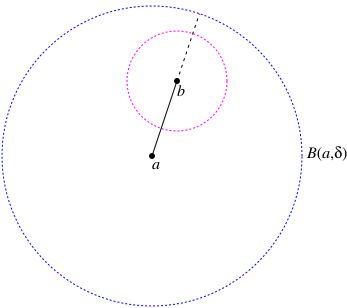
\includegraphics{Open_ball_neighborhood}}
\caption{$B(a, \delta)$ as a neighborhood of $b$.} 
\label{F:Open_ball_neighborhood}
\end{center}
\end{figure}

\item Is the converse true? That is, if a set is a neighborhood of each of its points, is the set an open ball? No proof is necessary, but a convincing argument is in order. 

\ea

\end{activity}

\begin{comment}

\ActivitySolution
\ba
\item We need to show that there is an open ball around $b$ that is entirely contained in $B(a, \delta)$. 


\item Let $\beta = d(a,b)$ and let $\gamma = \delta - \beta$. Let $c \in B(b,\gamma)$. Then 
\[d(a,c) \leq d(a,b) + d(b,c) < \beta + \gamma = \beta + (\delta - \beta) = \delta.\]
So $c \in B(a,\delta)$ and $B(b,\gamma) \subset B(a,\delta)$.  

\item This statement is not true. Consider $A = (0,1) \cup (2,3)$ as a subset of $\R$ with the Euclidean metric. The set $A$ is a neighborhood of each of its points, but $A$ is not an open ball -- rather $A$ is the union of two disjoint open balls. 

\ea

\end{comment}

\csection{Continuity and Neighborhoods}\label{sec_cont_neighborhoods}
We can define continuity now in terms of neighborhoods instead of using metrics. The advantage here is that this idea does not explicitly depend on the existence of a metric, so we will be able to adopt this concept of continuity for arbitrary topological spaces. 

Recall that a function $f$ from a metric space $(X, d_X)$ to a metric space $(Y, d_Y)$ is continuous at $a \in X$ if, for any $\epsilon > 0$ there exists $\delta > 0$ so that $d_X(x,a) < \delta$ implies $d_Y(f(x),f(a)) < \epsilon$. We can interpret this definition of continuity to say that for every $\epsilon > 0$, the inverse image under $f$ of the open ball $B(f(a), \epsilon)$ contains the open ball $B(a, \delta)$ for some $\delta > 0$. It is not unreasonable to wonder if the set $f^{-1}\left(B(f(a), \epsilon)\right)$ itself is an open ball. We investigate this question in the following activity. 

\begin{activity} \label{act:OB_1} Let $f$ be a function from a metric space $(X, d_X)$ to a metric space $(Y, d_Y)$ that is continuous at $a \in X$. Using the notation from the paragraph above, in this activity we determine if $f^{-1}\left(B(f(a), \epsilon)\right)$ must equal $B(a, \delta)$ for some $\delta$.

Define $f : \R \to \R$ by 
\[f(x) = x^2,\]
where we use the Euclidean metric $d_E$ throughout.  Assume that $f$ is a continuous function.  Then $f$ is continuous at $x=2$.
\ba
\item What is $B(f(2), 1)$? 

\item What is $f^{-1}\left(B(f(2), 1)\right)$?

\item Is $f^{-1}\left(B(f(2), 1)\right)$ an open ball centered at $2$? Explain.

\ea

\end{activity}
 
\begin{comment}

\ActivitySolution
\ba
\item The set $B(f(2),1)$ is the interval $(f(2)-1,f(2)+1) = (3,5)$ in $\R$.

\item The set of points in $\R$ that map into $B(f(2),1)$ is the interval $(\sqrt{3}, \sqrt{5})$. 

\item Since $\sqrt{5} - 2 \approx 0.236$ and $2 - \sqrt{3} \approx 0.2679$, the set $f^{-1}\left(B(f(2), 1)\right)$ only contains an open ball centered at $2$, but is not itself an open ball centered at 2. 

\ea

\end{comment}

The conclusion to be drawn from Activity \ref{act:OB_1} is that if $f$ is continuous, we can only conclude that the inverse image of $B(f(a), \epsilon)$ \emph{contains} an open ball centered at $a$. By definition of continuity, if for every $\epsilon > 0$ there exists a $\delta > 0$ so that the open ball $f^{-1}\left(B(f(a), \epsilon)\right)$ contains $B(a, \delta)$, then $f$ is continuous at $a$. We summarize this in the next theorem.


\begin{theorem} \label{thm:open_ball_continuity} Let $f$ be a function a metric space $(X, d_X)$ to a metric space $(Y, d_Y)$, and let $a \in X$. Then $f$ is continuous at $a \in X$ if and only if, given any $\epsilon > 0$ there exists $\delta > 0$ so that 
\[B(a, \delta) \subseteq f^{-1}\left(B(f(a), \epsilon)\right).\]
\end{theorem}

We can extend this idea of continuity to describe continuity in terms of neighborhoods. This condition will allow us to later consider continuous functions even if there are no metrics on our spaces. 

\begin{theorem} Let $(X, d_X)$ and $(Y,d_Y)$ be metric spaces, and let $f : X \to Y$ be a function. Then $f$ is continuous at $a \in X$ if and only if the inverse image of every neighborhood of $f(a)$ is a neighborhood of $a$. 
\end{theorem}

\begin{proof} Let $(X, d_X)$ and $(Y,d_Y)$ be metric spaces, and let $f : X \to Y$ be a function. To prove this biconditional statement we need to prove both implications. First assume that $f$ is continuous at some point $a \in X$. We will show that for any neighborhood $N$ of $f(a)$ in $Y$, its inverse image $f^{-1}(N)$ in $X$ is a neighborhood of $a$ in $X$. Let $N$ be a neighborhood of $f(a)$ in $Y$. To demonstrate that $f^{-1}(N)$ is a neighborhood of $a$ in $X$, we need to find an open ball around $a$ that is contained in $f^{-1}(N)$. Since $N$ is a neighborhood of $f(a)$, by definition there exists $\epsilon > 0$ so that $B(f(a), \epsilon) \subseteq N$. Since $f$ is continuous at $a$, there exists $\delta > 0$ such that $B(a, \delta) \subseteq f^{-1}\left(B(f(a), \epsilon)\right)$. So if $x \in B(a, \delta)$, then $f(x) \in B(f(a), \epsilon) \subseteq N$. So $B(a, \delta) \subseteq f^{-1}(N)$, and $f^{-1}(N)$ is a neighborhood of $a$ in $X$. 

The proof of the reverse implication is left for the next activity.
\end{proof}



\begin{activity} Let $(X, d_X)$ and $(Y,d_Y)$ be metric spaces, and let $f : X \to Y$ be a function. Let $a \in X$. In this activity we prove that if the inverse image of every neighborhood of $f(a)$ is a neighborhood of $a$, then $f$ is continuous at $a$.
\ba
\item What does Theorem \ref{thm:open_ball_continuity} tell us that we need to do to show that $f$ is continuous at $a$?

\item Suppose $\epsilon$ is greater than 0, why is $B(f(a), \epsilon)$ a neighborhood of $f(a)$ in $Y$?

\item What does our hypothesis tell us about $f^{-1}\left(B(f(a), \epsilon)\right)$?

\item What can we conclude from part (c)?

\item How do (a)-(d) show that $f$ is continuous at $a$?

\ea

\end{activity}

\begin{comment}

\ActivitySolution
\ba
\item We need to show that the inverse image of any open ball centered at $f(a)$ contains an open ball centered at $a$.

\item We showed earlier that an open ball is a neighborhood of each of its points.

\item Our hypothesis tells us that $f^{-1}\left(B(f(a), \epsilon)\right)$ is a neighborhood of $a$ in $X$. 

\item As a neighborhood of $a$, it follows that there exists $\delta > 0$ such that $B(a, \delta) \subseteq f^{-1}\left(B(f(a), \epsilon)\right)$. 

\item The previous parts show that given any $\epsilon > 0$ there exists $\delta > 0$ such that $B(a, \delta) \subseteq f^{-1}\left(B(f(a), \epsilon)\right)$. Theorem \ref{thm:open_ball_continuity} then shows that $f$ is continuous at $a$. 

\ea

\end{comment}

\noindent We conclude this section with some important facts about neighborhoods. Assume that $(X,d)$ is a metric space and $a \in X$. 

\begin{itemize}
\item There is a neighborhood that contains $a$.
\item If $N$ is a neighborhood of $a$ and $N \subseteq M$, then $M$ is a neighborhood of $a$.
\item If $M$ and $N$ are neighborhoods of $a$, then so is $M \cap N$.
\end{itemize}

The proofs are straightforward and left for Exercise (\ref{ex:Nghb_properties}).

\csection{Summary}\label{sec_open_balls_summ}
Important ideas that we discussed in this section include the following.
\begin{itemize}
\item If $(X,d)$ is a metric space and $a \in X$, then an open ball centered at $a$ is a set of the form
\[B(a,\delta) = \{ x \in X \mid d(x,a) < \delta\}\]
for some positive number $\delta$. 
\item A subset $N$ of a metric space $(X,d)$ is s neighborhood of a point $a \in N$ if there is a positive real number $\delta$ such that $B(a,\delta) \subseteq N$.
\item An important property of open balls is that every open ball is a neighborhood of each of its points. This is our first step toward defining the concept of open sets that will form the foundation for topological spaces. 
\item A function $f$ from a metric space $(X,d_X)$ to a metric space $(Y,d_Y)$ is continuous at $a \in X$ if $f^{-1}(N)$ is a neighborhood of $a$ in $X$ for any neighborhood $N$ of $f(a)$ in $Y$. 
\end{itemize}


\csection{Exercises}\label{sec_open_balls_exer}

\be

\item Determine, with proof, which of the following sets $A$ is a neighborhood of $a$ in the indicated metric space. 

\ba

\item $A = \{(x,y) \in \R^2 \mid x^2+y^2 < 1\}$ in $(\R^2,d_E)$ with $a = (0.5,0.5)$

\item $A$ is the $x$-axis in $(\R^2,d_T)$ with $a =(0,0)$, where $d_T$ is the taxicab metric

\item $A$ is the set of rational numbers in $(\R, d_E)$ with $a = 0$

\item $A$ is the set of positive integers in $(Q,d)$ and $a = 1$, where $Q$ is the set of all rational numbers in reduced form with metric $d : Q \times Q \to \R$ defined by 
\[d\left(\frac{a}{b}, \frac{c}{d}\right) = \max\{| a-c |, | b-d |\}\]
(The fact that $d$ is a metric is the topic of Exercise \ref{ex:MS_Q_metric} on page \pageref{ex:MS_Q_metric}.)


\ea

\begin{comment}

\ExerciseSolution

\ba

\item Since $A = B((0,0),1)$ and we know that every open ball is a neighborhood of each of its points, we conclude that $A$ is a neighborhood of $a$. 

\item Let $\delta$ be a positive real number and consider the open ball $B(a, \delta)$ in $(\R^2,d_T)$. The point $\left(0, \frac{\delta}{2}\right)$ is in $B(a,\delta)$ but not in $A$. So $A$ cannot contain any open ball centered at $a$. We conclude that $A$ is not a neighborhood of $a$.  

\item Exercise \ref{ex:GLB_irrational} on page \pageref{ex:GLB_irrational} tells us that there is an irrational number between any two real numbers. So there are irrational numbers in any interval of the form $(a - \delta, a+\delta)$ for any $\delta > 0$. We conclude that $A$ is not a neighborhood of $a$. 

\item Consider the ball $B(a,1)$ in $Q$. An element $\frac{p}{q}$ is in $B(a,1)$ if 
\[d\left(\frac{1}{1}, \frac{p}{q}\right) = \max\{| 1-p |, | 1-q |\} < 1.\]
This can only happen if $|1-p| < 1$ and $|1-q| < 1$. But $p$ and $q$ are integers, so we must have $p = q = 1$. Thus, $B(a,1) = \{a\}$. So any set that contains $a$ in $Q$ contains $B(a,1)$. We conclude that any set that contains $a$ is a neighborhood of $a$.   

\ea

\end{comment}


\item Let $X = \{1,3,5\}$ and define $d_X: X \times X \to \R$ by $d_X(x,y) = xy - 1 \pmod{8}$. That is, $d_X(x,y)$ is the remainder when $xy - 1$ is divided by $8$. That $d_X$ is a metric on $X$ is examined in Exercise \ref{ex:MS_mod_metric} on page \pageref{ex:MS_mod_metric}. Let $(Y,d_Y)$ be a metric space. Is it possible to define a function $f: X \to Y$ that is not continuous? Explain. 

\begin{comment}

\ExerciseSolution Recall that $d_X$ has values as in Table \ref{T:open_balls_example_8}.
\begin{table}[h]
\begin{center}
\begin{tabular}{|c|c|c|c|} \hline
	&$1$	&$3$	&$5$	\\ \hline
$1$	&$0$	&$2$	&$4$	\\ \hline
$3$	&$2$	&$0$	&$6$	\\ \hline
$5$	&$4$	&$6$	&$0$	\\ \hline
\end{tabular}
\caption{Values of $d_X$.}
\label{T:open_balls_example_8}
\end{center}	
\end{table}
Notice that $B(x,1) = \{x\}$ for every $x \in X$. So if $f: X \to Y$ is a function and $N$ is a neighborhood of $f(x)$ in $Y$, then $B(x,1) \subseteq f^{-1}(N)$. So $f^{-1}(N)$ is a neighborhood of $x$ for every $x \in X$ and $f$ must be a continuous function. 

\end{comment}
	

\item If $x = (x_1, x_2, \ldots, x_n)$, we let $|x| = \sqrt{x_1^2+x_2^2+ \cdots + x_n^2}$. For $x = (x_1, x_2, \ldots, x_n)$ and $y = (y_1, y_2, \ldots y_n)$, define $d_H: \R^n \times \R^n \to \R$ by 
\[d_H(x,y) = \begin{cases} 0 &\text{ if } x=y \\ |x|+|y| &\text{ otherwise}. \end{cases}\]
The fact that $d_H$ is a metric is examined in Exercise \ref{ex:MS_hub} on page \pageref{ex:MS_hub}. 

Let $(X,d_X) = (\R^2, d_H)$ and let $(Y,d_Y) = (\R, d_E)$. Define $f: X \to Y$ and $g: X \to Y$ by 
\[f(x) = \begin{cases} 0 &\text{ if } x = (0,0) \\ 1 &\text{ otherwise} \end{cases} \  \text{ and } \ g(x) = \begin{cases} 0 &\text{ if } |x|<1 \\ 1 &\text{ otherwise} \end{cases}.\]
One of $f$, $g$ is continuous and the other is not. Determine which is which, with proof for each. 

\begin{comment}

\ExerciseSolution Let $B = B(0,1)$ in $Y$. Notice that $f^{-1}(B) = \{(0,0)\}$. Now $B((0,0),r) = \{x \in \R^2 \mid |x|<r\}.$ So the only way $B((0,0),r) = f^{-1}(B)$ is if $r=0$. Thus, $f^{-1}(B)$ is not a neighborhood of $(0,0)$ and so $f$ is not continuous. 

Now we show that $g$ is continuous. Let $a = (a_1,a_2) \in X$. We demonstrate that $g$ is continuous at $a$. By the definition of $g$, we either have $g(a) = 0$ or $g(a) = 1$. We consider the cases.
\begin{description}
\item[Case 1: $g(a) = 0$.] In this case we have $|a| < 1$. Let $B = B(g(a),\epsilon) = B(0,\epsilon) = (-\epsilon, \epsilon)$. Let $\delta = \frac{3|a|}{2}$. If $x$ is in $B(a,\delta)$, then 
\begin{align*}
d_H(a,x) &< \delta \\
|a|+|x| &<  \frac{3|a|}{2} \\
|x| &< \frac{|a|}{2} < 1.
\end{align*}
So we must have $g(x) = 0$ as well. Thus,
\[|g(a) - g(x)| = |0-0|  = 0 <  \epsilon.\]
We conclude that $g$ is continuous at $a$ when $g(a) = 0$. 
    
\item[Case 2: $g(a) = 1$.] Here we have $|a| \geq 1$. Let $\delta = |a|$. If $x$ is in $B(a,\delta)$, then 
\begin{align*}
d_H(a,x) &< \delta \\
|a|+|x| &<  |a| \\
|x| < 0.
\end{align*}
But then $B(a,\delta) = \{a\}$ and $B(a,\delta) \subseteq g^{-1}(B(g(a),\epsilon)$. We conclude that $g$ is continuous at $a$ when $g(a) = 1$. 
\end{description} 

\end{comment}

\item Recall from Section \ref{sec:metric_spaces} that we can construct a finite metric space by starting with a finite set of points and making a graph with the points as vertices. We construct edges so that the graph is connected (that is, there is a path from any one vertex to any other) and give weights to the edges. We then define a metric $d$ on $S$ by letting $d(x,y)$ be the length of a shortest path between vertices $x$ and $y$ in the graph. \\

Consider the metric space $(X,d)$ corresponding to the graph in Figure \ref{F:Graph_metric_ex}. 
\begin{figure}[h]
\begin{center}
\resizebox{!}{2.0in}{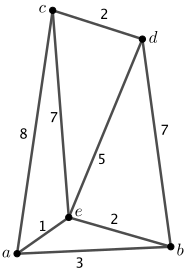
\includegraphics{Graph_metric.eps}}
\caption{A graph to define a metric.} 
\label{F:Graph_metric_ex}
\end{center}
\end{figure}
\ba
\item Determine all of the open balls $B(a,\delta)$ for every positive real number $\delta$. 

\item Find all of the neighborhoods of $a$. 

\ea

\begin{comment}

\ExerciseSolution

\ba

\item First we list the distances from $a$ to the other points in $X$:
\begin{center}
\begin{tabular}{c|cccc}
$x$		&$b$	&$c$&$d$&$e$ \\
$d(a,x)$	&$3$&$8$&$6$&$1$
\end{tabular}
\end{center}
So 
\begin{itemize}
\item if $\delta \leq 1$, then $B(a,\delta) = \{a\}$; \\
\item if $1< \delta \leq 3$, then $B(a,\delta) = \{a,e\}$; \\
\item if $3< \delta \leq 6$, then $B(a,\delta) = \{a,b,e\}$; \\
\item if $6< \delta \leq 8$, then $B(a,\delta) = \{a,b,d,e\}$; \\
\item if $8< \delta$, then $B(a,\delta) =X$.
\end{itemize}

\item Every neighborhood of $a$ must contain $a$, and if $A$ is a subset of $X$ that contains $a$, then $B(a,1) = \{a\}$ is a subset of $A$. So the neighborhoods of $a$ are the subsets of $X$ that contain $a$.  

\ea

\end{comment}

\item \label{ex:linear_continuous}
	\ba
	\item Let $f: (\R,d_E) \to (\R,d_E)$ be defined by $f(x) = ax+b$ for some real numbers $a$ and $b$ with $a \neq 0$. Let $p \in \R$ and let $r > 0$. Show that $f^{-1}(B(f(p),r))$ contains an open ball centered at $p$. Conclude that every linear function from $(\R,d_E)$ to $(\R,d_E)$ is continuous. (Hint: By Exercise \ref{ex:sum_continuous} on page \pageref{ex:sum_continuous} we can assume $a > 0$ to simplify the problem.)
	
	\item Let $f: (\R,d_E) \to (\R,d_E)$ be defined by $f(x) = ax^2+bx+c$ for some real numbers $a$, $b$, and $c$ with $a \neq 0$. Let $p \in \R$ and let $r > 0$. $f^{-1}(B(f(p),r))$ contains an open ball centered at $p$. Conclude that every quadratic function from $(\R,d_E)$ to $(\R,d_E)$ is continuous. (Hint: Consider cases.)
	
	\ea
	
\begin{comment}

\ExerciseSolution

\ba

\item Let $f(x) = ax+b$ for some real numbers $a$ and $b$ with $a > 0$. Let $p \in \R$ and let $r > 0$. Then $f^{-1}(B(f(p),r) = B\left(p, \frac{r}{m}\right)$ and so $f$ is continuous at $x=p$. Since $f$ is continuous at every real input, $f$ is a continuous function. 

\item Let $f(x) = ax^2+bx+c$ for some real numbers $a$, $b$, and $c$ with $a > 0$. Notice that $f$ attains its minimum value of $f(m) = c-\frac{b^2}{4a}$ at $m = -\frac{b}{2a}$. Let $p \in \R$ and let $r > 0$. We consider cases.
\begin{description}
\item[$p > m$:] Let $r' = \min\{r, |f(p)-f(m)|\}$. Then $B(f(p),r') \subseteq B(f(p),r)$ and $f^{-1}(B(f(p),r')) \subseteq (m, \infty)$. So there exist unique $x_1$, $x_2$ in $(m, \infty)$ such that $f(x_1) = f(p)-r'$ and $f(x_2) = f(p)+r'$. Let $s = \min\{p-x_1, x_2-p\}$. Then $B(p,s) \subseteq f^{-1}(B(f(p), r') \subseteq f^{-1}(B(f(p), r)$. 

\item[$p < m$:] Let $r' = \min\{r, |f(p)-f(m)|\}$. Then $B(f(p),r') \subseteq B(f(p),r)$ and $f^{-1}(B(f(p),r')) \subseteq (-\infty,m)$. So there exist unique $x_1$, $x_2$ in $(m, \infty)$ such that $f(x_1) = f(p)+r'$ and $f(x_2) = f(p)-r'$. Let $s = \min\{p-x_1, x_2-p\}$. Then $B(p,s) \subseteq f^{-1}(B(f(p), r') \subseteq f^{-1}(B(f(p), r)$. 

\item[$p = m$:] In this case there exist $x_1$, $x_2$ in $\R$ such that $f(x_1) = f(p)+r = f(x_2)$ and $x_1 < x_2$. Let $s = p-x_1$. Then $B(p,s) \subseteq f^{-1}(B(f(p), r)$. 

\end{description}

In each case, the inverse image of any open ball that has $f(p)$ as an element contains an open ball that has $p$ as an element. We conclude that $f$ is a continuous function. 

\ea

\end{comment}

\item \label{ex:metric_continuous} Let $(X,d)$ be a metric space, and let $A$ be a nonempty subset of $X$. Exercise \ref{ex:GLB_triangle} on page \pageref{ex:GLB_triangle} tells us that 
\[d(b,A) \leq d(b,c) + d(c,A)\]
 for all $b, c \in X$. 

Define $f: X \to \R$ by $f(x) = d(x,A)$. Let $b \in X$. Given $\epsilon > 0$, show that there is a neighborhood $N$ of $b$ such that $x \in N$ implies $f(x) \in B(f(b),\epsilon)$. Conclude that $f$ is a continuous function. (Assume the metric on $\R$ is the Euclidean metric.)


\begin{comment}

\ExerciseSolution Define $f: X \to \R$ by $f(x) = d(x,A)$. Let $b \in X$ and let $\epsilon$ be greater than $0$. Let $N = B(b, \epsilon)$.  We know that $N$ is a neighborhood of $b$. Suppose $x \in N$. Part i. shows that  
\[d(b,A) \leq d(b,x) + d(x,A) < \epsilon+d(x,A).\]
 So $d(b,A) - d(x,A) < \epsilon$ and $-\epsilon < d(x,A) - d(b,A)$. It follows that $|d(b,A) - d(x,A)| < \epsilon$ and $f(x) \in B(f(a),\epsilon)$.  This shows that $f$ is a continuous function.  


\end{comment}


\item Let $a$ and $b$ be distinct points of a metric space $X$. Prove that there are neighborhoods $N_a$ and $N_b$ of $a$ and $b$ respectively such that $N_a \cap N_b = \emptyset$.  

\begin{comment}

\ExerciseSolution Let $a$ and $b$ be distinct points of a metric space $(X,d)$. Since $a \neq b$, we know that $d(a,b) > 0$. Let $r = \frac{d(a,b)}{2}$. By definition, $N_a = B(a; r)$ and $N_b = B(b; r)$ are neighborhoods of $a$ and $b$ respectively. We will show that the intersection of $N_a$ and $N_b$ is empty. Assume to the contrary that there is an element $x$ in $N_a \cap N_b$. Then $d(x,a) < r$ and $d(x,b) < r$. It follows that 
\[d(a,b) \leq d(a,x) + d(x,b) < r + r = 2r = d(a,b).\]
Since this is impossible, we conclude that $N_a \cap N_b = \emptyset$ as desired. 

\end{comment}

\item \label{ex:Nghb_properties} Let $(X,d)$ be a metric space and let $a \in X$. Prove each of the following.

\ba
\item There is a neighborhood that contains $a$.
\item If $N$ is a neighborhood of $a$ and $N \subseteq M$, then $M$ is a neighborhood of $a$.
\item If $M$ and $N$ are neighborhoods of $a$, then so is $M \cap N$.
\ea

\begin{comment}

\ExerciseSolution

\ba

\item Every ball is a neighborhood of each of its points, so $B(a,1)$ is a neighborhood of $a$ that contains $a$.

\item Since $N$ contains an open ball $B$ that contains $a$, we have that $B \subseteq N \subseteq M$ and $M$ contains an open ball that contains $a$. So $M$ is a neighborhood of $a$.

\item Suppose $M$ and $N$ are neighborhoods of $a$. Then there are open balls $B(a,m) \subseteq M$ and $B(a,n) \subseteq N$ for some positive real numbers $m$ and $n$. Then $B(a, \min\{m,n\}) \subseteq B(a,m) \cap B(a,n) \subseteq M \cap N$. Thus, $M \cap N$ is a neighborhood of $a$. 

\ea

\end{comment}
 
\item Let $f: (\R,d_E) \to (\R,d_E)$ be a continuous function. Show that if $f(a) > 0$ for some $a \in \R$, then there is a neighborhood $N$ of $a$ such that $f(x) > 0$ for all $x \in N$. 

\begin{comment}

\ExerciseSolution Assume that $f: (\R,d_E) \to (\R,d_E)$ is continuous and suppose $f(a) > 0$ for some $a \in \R$. There exists $\delta > 0$ such that $|x - a| < \delta$ implies $|f(x)-f(a)| < f(a)$. It follows that $-f(a) < f(x)-f(a) < f(a)$ or $0 < f(x) < 2f(a)$. Thus, $f(x) > 0$ for all $x$ in $B(a, \delta)$. 

\end{comment}

\item Let $(X,d)$ be a metric space where $d$ is the discrete metric. Show that every subset of $X$ is a neighborhood of each of its points.

\begin{comment}

\ExerciseSolution Let $A$ be a subset of $X$ and let $a \in A$. Since $B(a,1) = \{a\} \subseteq A$, we see that $A$ is a neighborhood of each of its points. 

\end{comment}

\item For each of the following, answer true if the statement is always true. If the statement is only sometimes true or never true, answer false and provide a concrete example to illustrate that the statement is false. If a statement is true, explain why. 

	\ba
	\item If $N$ is a neighborhood of a point $a$ in a metric space $X$, then any open ball contained in $N$ is also a neighborhood of $a$. 

	\item If $N$ is a neighborhood of a point $a$ in a metric space $X$, then $N$ is a neighborhood of each of its points. 	
		
	\item If $X$ and $Y$ are metric spaces and $f : X \to Y$ is a continuous function, then $f(N)$ is a neighborhood of $f(a)$ in $Y$ whenever $N$ is a neighborhood of $a$ in $X$. 
	
	\item If $X$ and $Y$ are metric spaces and $f : X \to Y$ is continuous at $a \in X$, and $N$ is a neighborhood of $f(a)$ in $Y$, then $f^{-1}(N)$ is a neighborhood of $a$ in $X$.
	
	\item If $a$ is a point in a metric space $X$ and if $\delta$ is a positive real number, then the open ball $B(a,\delta)$ contains infinitely many points of $X$.

	\item If $N_1$, $N_2$, $\ldots$, $N_k$ are neighborhoods of a point $a$ in a metric space $X$ for some positive integer $k$, then $\bigcap_{i=1}^k N_i$ is a neighborhood of $a$.  
	
	\item If $N_{\alpha}$ is a neighborhood of a point $a$ in a metric space $X$ for all $\alpha$ in some indexing set $I$, then $\bigcap_{\alpha \in I} N_{\alpha}$ is a neighborhood of $a$.  
	
	\ea

\begin{comment}

\ExerciseSolution

\ba

\item This statement is false. Let $(X, d_X) = (\R, d_E)$. Then $N = B(3,3) = (0,6)$ is a neighborhood of $a=3$, but $B(1,1) \subset N$ does not contain $3$ and is not a neighborhood of $3$.  
	 
	\item This statement is false. Let $(X, d_X) = (\R, d_E)$. The set $N = [0,2]$ is a neighborhood of $1$, since $B(1,1) \subset N$. However, if $B(c,r)$ contains $0$ for some $c \in N$ and some $r > 0$, then $d_E(0,c)  = c < r$. So if $x = \frac{c-r}{2}$, then since all of our points lie on the line $\R$ we have 
	\[d_E(x,c) = |c-x| = c-\left(\frac{c-r}{2}\right) = \frac{c+r}{2} < \frac{r+r}{2} = r.\]
So $x \notin N$ and it follows that $N$ contains no open ball containing $0$. Thus, $N$ is not a neighborhood of $0$. 

	\item This statement is false. Let $X = Y = \R$ with the Euclidean metrics, and let $f(x) = 0$ for all $x \in \R$. We know that constant functions are continuous. Then $N = B(0,1)$ is a neighborhood of $0$, but $f(N) = \{0\}$ does not contain any open balls and so is not a neighborhood of $f(0)$. 

	\item This statement is true since it is just a restatement of a theorem about continuous functions.

	\item This statement is false. Let $X = \R$ and $d$ be the discrete metric. Then $B(0,1) = \{0\}$. 
		
	\item This statement is true. Each $N_i$ contains an open ball that contains $a$. Since an open ball is a neighborhood of each of its points, for each $i$ there is an open ball $B(a,r_i)$ contained in $N_i$. If we let $r = \min\{r_i \mid 1 \leq i \leq k\}$, then $r > 0$ and $B(a,r) \subseteq B(a,r_i) \subseteq N_i$ for each $i$. Thus, $B(a,r) \subseteq \bigcap_{i=1}^k N_i$. 	

	\item This statement is false. Let $I = \Z^+$ and for each $k \in I$ let $N_k = \left(-\frac{1}{k}, \frac{1}{k}\right)$. Then $N_k$ is a neighborhood of $0$ for each $k \in I$. However, $\bigcap_{\alpha \in I} N_{\alpha} = \{0\}$ is not a neighborhood of $0$ because $\{0\}$ contains no open ball of positive radius. 

\ea





\end{comment}

\ee

  %7
\achapter{8}{Open Sets in Metric Spaces}\label{sec:open_sets}


\vspace*{-17 pt}
\framebox{
\parbox{\dimexpr\linewidth-3\fboxsep-3\fboxrule}
{\begin{fqs}
\item What is an open set in a metric space?
\item What is an interior point of a subset of a metric space? How are interior points related to open sets?
\item What is the interior of a set? How is the interior of a set related to open sets?
\item How can we use open sets to determine the continuity of a function?
\item What important properties do open sets have in relation to unions and intersections?
\end{fqs}}}

\vspace*{13 pt}

\csection{Introduction}

Consider the interval $(a,b)$ in $\R$ using the Euclidean metric. If $m = \frac{a+b}{2}$, then $(a,b) = B\left(m,\frac{b-a}{2}\right)$, so every open interval is an open ball. As an open ball, an open interval $(a,b)$ is a neighborhood of each of its points. This is the foundation for the definition of an open set in a metric space. 

Recall that we defined a subset $N$ of $X$ to be neighborhood of point $a$ in a metric space $(X,d)$ if $N$ contains an open ball $B(a, \epsilon)$ for some $\epsilon > 0$. We saw that every open ball is a neighborhood of each of its points, and we will now extend that idea to define an \emph{open set} in a metric space.

\begin{definition} A subset $O$ of a metric space $X$ is an \textbf{open set}\index{open set in a metric space} if $O$ is a neighborhood of each of its points.
\end{definition}

So, by definition, any open ball is an open set. Also by definition, open sets are neighborhoods of each of their points. Open sets are different than non-open sets. For example, $(0,1)$ is an open set in $\R$ using the Euclidean metric, but $[0,1)$ is not. The reason $[0,1)$ is not an open set is that there is no open ball centered at $0$ that is entirely contained in $[0,1)$. So $0$ has a different property than the other points in $[0,1)$. The set $[0,1)$ is a neighborhood of each of the points in $(0,1)$, but is not a neighborhood of $0$. We can think of the points in $(0,1)$ as being in the interior of the set $[0,1)$. This leads to the next definition. 

\begin{definition} Let $A$ be a subset of a metric space $X$. A point $a \in A$ is an \textbf{interior point}\index{interior point in a subset of a metric space} of $A$ if $A$ is a neighborhood of $a$.
\end{definition}

As we will soon see, open sets can be characterized in terms of interior points. 

\begin{pa} ~
\be
\item Determine if the set $A$ is an open set in the metric space $(X,d)$. Explain your reasoning.
	\ba
	\item $X = \R$, $d = d_E$, the Euclidean metric, $A = [0,0.5)$.

	\item $X = \{x \in \R \mid 0 \leq x \leq 1\}$, $d = d_E$, the Euclidean metric, $A = [0,0.5)$. Assume that the Euclidean metric is a metric on $X$. 

	\item $X = \{a,b,c,d\}$, $d$ is the discrete metric defined by 
\[d(x,y) = \begin{cases} 0 &\text{if } x = y \\ 1 &\text{if } x \neq y, \end{cases}\]
and $A = \{a,b\}$. 

	\ea

\item ~
	\ba
	\item What are the interior points of the following sets in $(\R, d_E)$? Explain. 
	\[(0,1) \ \ \ (0,1] \ \ \ [0,1) \ \ \ [0,1].\]

	\item Let $A = \{0, 1, 2\}$ in $(\R, d_E)$. What are the interior points of $A$? Explain.
	
	\item Let $\Q$ be the set of rational numbers in $(\R, d_E)$. What are the interior points of $\Q$? Explain.
	
	\ea
\ee

\end{pa}

\begin{comment}

\ActivitySolution

\be
\item Determine if the set $A$ is an open set in the metric space $(X,d)$. Explain your reasoning.
	\ba
	\item The set $A$ is not an open set in $X$. Note that $0 \in A$, but the open ball of radius $\epsilon$ in $\R$ centered at $0$ has the form $(-\epsilon, \epsilon)$. So not open ball in $\R$ centered at $0$ is entirely contained in $A$. Thus, $A$ is not a neighborhood of $0$ and $A$ is not an open set.  

	\item  The set $A$ is an open set in $X$. Note that every open ball in $X$ must be contained in $X$. So the open ball of radius $0.25$ in $X$ centered at $0$ has the form $[0, 0.25)$, which is entirely contained in $A$. If $a$ is any point of $A$ other than $0$, then the open ball centered at $a$ of radius $\min\{a, 0.5-a\}$ is contained in $A$. So $A$ is a neighborhood of each of its points and $A$ is an open set. 

	\item  Notice that if $x \in X$, then $B(x, 0.5) = \{x\}$. So $A$ contains the open balls $B(a, 0.5)$ and $B(b, 0.5)$. Thus, $A$ is a neighborhood of each of its points and $A$ is an open set. 

	\ea

\item ~
	\ba
	\item  If $0 < a < 1$, then each of these sets contains the ball $B(a, \min\{a, 1-a\})$. So every point in $(0,1)$ is an interior point of each set. Note that any open ball $B(0,r)$ contains $-\frac{r}{2}$ and any open ball $B(1,r)$ contains the point $1+\frac{r}{2}$. These points are not in any of the sets, so $0$ and $1$ are not interior points of any of these sets.

	\item Let $r > 0$. Since $B(0,r)$ contains $\min\left\{0.25, \frac{r}{2}\right\}$, $B(1,r)$ contains $\min\left\{1.25, 1+\frac{r}{2}\right\}$, and $B(2,r)$ contains $\min\left\{2.25, 2+\frac{r}{2}\right\}$, we see that no point in $A$ is an interior point of $A$. 
	
	\item  Let $q \in \Q$, and let $r > 0$. If $r$ is irrational, the ball $B(q,r)$ contains the irrational number $q+\frac{r}{2}$. If $r$ is rational, then the ball $B(q,r)$ contains the irrational number $q+\frac{r}{2\pi}$. In either case, the ball $B(q,r)$ contains a number that is not in $\Q$. Thus, no point of $\Q$ is an interior point of $\Q$.  
	
	\ea
\ee


\end{comment}


\csection{Open Sets}

Open sets are vitally important in topology. In fact, we will see later that every topological space is completely defined by its open sets. Recall that an open ball is an open set. There are other subsets that every metric space contains, and we might ask if they are open or not.  

\begin{activity} Let $X$ be a metric space.
\ba
\item Is $\emptyset$ an open set in $X$? Explain.

\item Is $X$ an open set in $X$? Explain.

\ea

\end{activity}

\begin{comment}

\ActivitySolution

\ba
\item Since $\emptyset$ contains no points, it follows that $\emptyset$ is a neighborhood of each of its points. So $\emptyset$ is an open set. 

\item Let $a \in X$. For any $\epsilon > 0$, the ball $B(a,\epsilon)$ is a subset of $X$. Thus, $X$ is a neighborhood of each of its points and $X$ is an open set in $X$. 

\ea

\end{comment}


We have defined open balls, and open balls are the canonical examples of open sets. In fact, as the following theorem shows, the open balls determine the open sets.

\begin{theorem} \label{thm:OS_1} Let $X$ be a metric space. A subset $O$ of $X$ is open if and only if $O$ is a union of open balls.
\end{theorem}

\begin{proof} Let $X$ be a metric space and $O$ a subset of $X$. To prove this biconditional statement we first assume that $O$ is an open set and demonstrate that $O$ is a union of open balls. Let $a \in O$. Since $O$ is open, there exists $\epsilon_a > 0$ so that $B(a, \epsilon_a) \subseteq O$. We will show that 
\[O = \bigcup_{a \in O} B(a, \epsilon_a).\]
By the way we chose $\epsilon_a$, $B(a, \epsilon_a) \subseteq O$ for every $a \in O$. So $\bigcup_{a \in O} B(a, \epsilon_a) \subseteq O$. For the reverse containment, let $x \in O$. Then $x \in B(x, \epsilon_x)$ and so $x \in \bigcup_{a \in O} B(a, \epsilon_a)$. Thus, $O \subseteq \bigcup_{a \in O} B(a, \epsilon_a)$. We conclude that $O$ is a union of open balls if $O$ is an open set.

The proof of the converse is left for the following activity.
\end{proof}


\begin{activity} Let $X$ be a metric space. To prove the remaining implication of Theorem \ref{thm:OS_1}, assume that a subset $O$ of $X$ is a union of open balls. 
\ba
\item What do we need to show to prove that $O$ is an open set?

\item Let $x \in O$. Why is there an open ball $B$ in $O$ that contains $x$?

\item Complete the proof to show that $O$ is an open set.

\ea

\end{activity}

\begin{comment}

\ActivitySolution
\ba
\item We need to show that $O$ is a neighborhood of each of its points. 

\item Let $x \in O$. Since $O$ is a union of open balls, there must be an open ball $B$ in $O$ that contains $x$.  

\item Since every ball is a neighborhood of each of its points, there exists $\epsilon > 0$ such that $B(x, \epsilon) \subseteq B \subseteq O$. Thus, $O$ is a neighborhood of each of its points and is therefore an open set.

\ea

\end{comment}

Theorem \ref{thm:OS_1} tells us that every open set is made up of open balls, so the open balls generate all open sets much like a basis of a vector space in linear algebra generates all of the elements of the vector space. For this reason we call the set of open balls in a metric space a \emph{basis} for the open sets of the metric space. We will discuss this idea in more detail in a subsequent section.

\csection{Unions and Intersections of Open Sets}

Once we have defined open sets we might wonder about what happens if we take a union or intersection of open sets. 

\begin{activity} \label{act:Open_union} ~
\ba
\item Let $A = (-2,1)$ and $B = (-1,2)$ in $(\R, d_E)$. 
	\begin{enumerate}[i.]
	\item Is $A \cup B$ open? Explain.
		
	\item Is $A \cap B$ open? Explain.
		
	\end{enumerate}
	
\item Let $X = \R$ with the Euclidean metric. Let $A_n = \left(1-\frac{1}{n}, 1+\frac{1}{n}\right)$ for each $n \in \Z^+$.
	\begin{enumerate}[i.]
	\item What is $\bigcup_{n \geq 1} A_n$? A proof is not necessary.
			
	\item Is $\bigcup_{n \geq 1} A_n$ open in $\R$? Explain.
	
	\item What is $\bigcap_{n \geq 1} A_n$? A proof is not necessary.
			
	\item Is $\bigcap_{n \geq 1} A_n$ open in $\R$? Explain.
		
	\end{enumerate}

\ea

\end{activity}

\begin{comment}

\ActivitySolution

\ba
\item Let $A = (-2,1)$ and $B = (-1,2)$ in $(\R, d_E)$. 
	\begin{enumerate}[i.]
	\item Let $a \in A \cup B$. Then $a \in (-2,1)$ or $a \in (-1,2)$. These open intervals are open balls, and so are neighborhoods of each of their points. Thus, $A \cup B$ is a neighborhood of each of its points. 
		
	\item In this case we have $A \cap B = (-1,1)$. Since $(-1,1)$ is an open ball, $(-1,1)$ is a neighborhood of each of its points. Thus, $A \cap B$ is a neighborhood of each of its points and $A \cap B$ is an open set. 
		
	\end{enumerate}
	
\item Let $X = \R$ with the Euclidean metric. Let $A_n = \left(1-\frac{1}{n}, 1+\frac{1}{n}\right)$ for each $n \in \Z^+$.
	\begin{enumerate}[i.]
	\item When $n = 1$ the interval is $(0,2)$. All intervals for $n > 1$ are contained in $(0,2)$, so $\bigcup_{n \geq 1} A_n = (0,2)$.
			
	\item Since $\bigcup_{n \geq 1} A_n$ is an open ball, it is also an open set $\R$? 
	
	\item Each interval $\left(1-\frac{1}{n}, 1+\frac{1}{n}\right)$ contains 1. However, we can make $n$ larger enough so that any integer not equal to 1 is not in $\left(1-\frac{1}{n}, 1+\frac{1}{n}\right)$. So $\bigcap_{n \geq 1} A_n = \{1\}$. 
			
	\item There is no open ball of positive radius contained in $\bigcap_{n \geq 1} A_n$, so $\bigcap_{n \geq 1} A_n$ is not open in $\R$.
		
	\end{enumerate}
	

\ea

\end{comment}

Activity \ref{act:Open_union} demonstrates that an arbitrary intersection of open sets is not necessarily open. However, there are some things we can say about unions and intersections of open sets.

\begin{theorem} Let $X$ be a metric space.
\begin{enumerate}
\item Any union of open sets in $X$ is an open set in $X$.
\item Any finite intersection of open sets in $X$ is an open set in $X$. 
\end{enumerate}
\end{theorem}

\begin{proof} Let $X$ be a metric space. To prove part 1, assume that $\{O_{\alpha}\}$ is a collection of open sets in $X$ for $\alpha$ in some indexing set $I$ and let $O = \bigcup_{\alpha \in I} O_{\alpha}$. By Theorem \ref{thm:OS_1}, we know that $O_{\alpha}$ is a union of open balls for each $\alpha \in I$. Combining all of these open balls together shows that $O$ is a union of open balls and is therefore an open set by Theorem \ref{thm:OS_1}. 

For part 2, assume that $O_1$, $O_2$, $\ldots$, $O_n$ are open sets in $X$ for some $n \in \Z^+$. To show that $O = \bigcap_{k=1}^n O_k$ is an open set, we will show that $O$ is a neighborhood of each of its points. Let $x \in O$. Then $x \in O_k$ for each $1 \leq k \leq n$. Let $k$ be between 1 and $n$. Since $O_k$ is open, we know that $O_k$ is a neighborhood of each of its points. So there exists $\epsilon_k > 0$ such that $B(x, \epsilon_k) \subseteq O_k$. Since there are only finitely many values of $k$, let $\epsilon = \min\{\epsilon_k \mid 1 \leq k \leq n\}$. Then $B(x, \epsilon) \subseteq B(x, \epsilon_k)$ for each $k$ and so $B(x, \epsilon) \subseteq \bigcap_{k=1}^n O_k = O$. Therefore, $O$ is a neighborhood of each of its points and $O$ is an open set.
\end{proof}


\csection{Continuity and Open Sets}
Recall that we showed that a function $f$ from a metric space $(X,d_X)$ to a metric space $(Y,d_Y)$ is continuous if and only if $f^{-1}(N)$ is a neighborhood of $a \in X$ whenever $N$ is a neighborhood of $f(a)$ in $Y$. We can now provide another characterization of continuous functions in terms of open sets. This is the characterization that will serve as our definition of continuity in topological spaces.

\begin{theorem} \label{thm:Open_continuity} Let $f$ be a function from a metric space $(X,d_X)$ to a metric space $(Y,d_Y)$. Then $f$ is continuous if and only if $f^{-1}(O)$ is an open set in $X$ whenever $O$ is an open set in $Y$.  
\end{theorem}

\begin{proof} Let $(X, d_X)$ and $(Y,d_Y)$ be metric spaces, and let $f : X \to Y$ be a function. To prove this biconditional statement we need to prove both implications. First assume that $f$ is a continuous function. We must show that $f^{-1}(O)$ is an open set in $X$ for every open set $O$ in $Y$. So let $O$ be an open set in $Y$. To demonstrate that $f^{-1}(O)$ is open in $X$, we will show that $f^{-1}(O)$ is a neighborhood of each of its points. Let $a \in f^{-1}(O)$. Then $f(a) \in O$. Now $O$ is an open set, so there is an open ball $B(f(a), \epsilon)$ around $f(a)$ that is entirely contained in $O$. Since $B(f(a), \epsilon)$ is a neighborhood of $f(a)$, we know that $f^{-1}(B(f(a), \epsilon))$ is a neighborhood of $a$. Thus, there exists $\delta > 0$ so that $B(a, \delta) \subseteq f^{-1}(B(f(a), \epsilon))$. Now $f(B(a, \delta)) \subseteq B(f(a), \epsilon) \subseteq O$, and so $B(a, \delta) \subseteq f^{-1}(O)$. We conclude that $f^{-1}(O)$ is a neighborhood of each of its points and is therefore an open set in $X$.

The proof of the reverse implication is left for the next activity.
\end{proof}


\begin{activity} Let $f$ be a function from a metric space $(X,d_X)$ to a metric space $(Y,d_Y)$. 
\ba
\item What assumption do we make to prove the remaining implication of Theorem \ref{thm:Open_continuity}? What do we need to demonstrate to prove the conclusion?

\item Let $a \in X$, and let $N$ be a neighborhood of $f(a)$ in $Y$. Why does there exist an $\epsilon > 0$ so that $B(f(a), \epsilon) \subseteq N$.

\item What does our hypothesis tell us about $f^{-1}(B(f(a), \epsilon))$ in $X$?

\item Why is $f^{-1}(N)$ a neighborhood of $a$? How does this show that $f$ is a continuous function? 

\ea

\end{activity}

\begin{comment}

\ActivitySolution

\ba
\item We assume that $f^{-1}(O)$ is an open set in $X$ whenever $O$ is an open set in $Y$. We need to show that for any $a \in X$, $f^{-1}(N)$ is a neighborhood of $a$ whenever $N$ is a neighborhood of $f(a)$. 

\item By definition of a neighborhood, there exists an $\epsilon > 0$ so that $B(f(a), \epsilon) \subseteq N$.

\item Now $B(f(a), \epsilon)$ is an open set in $Y$, so $f^{-1}(B(f(a), \epsilon))$ is an open set in $X$ by hypothesis.

\item  Every open set is a neighborhood of each of its points, and $a \in f^{-1}(B(f(a), \epsilon))$, so there exists $\delta > 0$ such that $B(a, \delta) \subseteq f^{-1}(B(f(a), \epsilon))$. Now $f(B(a, \delta)) \subseteq B(f(a), \epsilon) \subseteq N$, so $B(a, \delta) \subseteq f^{-1}(N)$. We conclude that $f^{-1}(N)$ is a neighborhood of $a$ and so $f$ is a continuous function. 

\ea

\end{comment}

Recall that every open set is a union of open balls, so we can simplify proofs of continuous functions in metric spaces by working only with open balls instead of arbitrary open sets. The next activity provides the details.

\begin{activity} \label{act:continuity_balls} In this activity we prove the following corollary to Theorem \ref{thm:Open_continuity}.

\begin{corollary} \label{cor:continuity_balls} A function $f$ from a metric space $(X,d_X)$ to a metric space $(Y,d_Y)$ is continuous if and only if $f^{-1}(B)$ is open in $X$ whenever $B$ is an open ball in $Y$.
\end{corollary}

To set up the proof, let $(X,d_X)$ and $(Y,d_Y)$ be metric spaces, and let $f: X \to Y$ be a function.

	\ba

	\item Since the corollary is a biconditional statement, we need to prove both implications. First, assume that $f$ is continuous. Use Theorem \ref{thm:Open_continuity} to explain why $f^{-1}(B)$ is open in $X$ whenever $B$ is an open ball in $Y$. 

\item For the remaining implication, assume that $f^{-1}(B)$ is an open set in $X$ for any open ball $B$ in $Y$. To show that $f$ is a continuous function, we will use Theorem \ref{thm:Open_continuity} and show that $f^{-1}(O)$ is open in $X$ whenever $O$ is an open set in $Y$. So let $O$ be an open set in $Y$. 
	\begin{enumerate}[i.]
	\item What does Theorem \ref{thm:OS_1} tell us about $O$. 
	
	\item Recall that Lemma \ref{lem:functions_subsets} tells us that if $\{B_{\beta}\}$ is a collection of subsets of $Y$ for $\beta$ in some indexing set $J$, then \[f^{-1}\left(\bigcup_{\beta \in J} B_{\beta}\right) = \bigcup_{\beta \in J} f^{-1}(B_{\beta}).\]
 Use Lemma \ref{lem:functions_subsets} to show that $f^{-1}(O)$ is open in $X$ and conclude that $f$ is a continuous function. 
 
 	\end{enumerate}

	\ea
	
\end{activity}

\begin{comment}

\ActivitySolution

\ba

\item Since $B$ is an open set and $f$ is continuous, Theorem shows that $f^{-1}(B)$ is an open set in $X$.

\item 
	\begin{enumerate}[i.]
	\item Theorem \ref{thm:OS_1} tells us that $O = \bigcup_{t \in I}B(t, \alpha_t)$ is a union of open balls in $Y$ for $t$ in some indexing set $I$. 
	
	\item By Lemma \ref{lem:functions_subsets} we have 
\[f^{-1}(O) = f^{-1}\left( \bigcup_{t \in I} B(t, \alpha_t) \right) = \bigcup_{t \in I} f^{-1}(B(t, \alpha_t)).\]
By hypothesis, $f^{-1}(B(t, \alpha_t)$ is an open set in $X$. Therefore, $f^{-1}(O)$ is a union of open sets in $X$ and so $f^{-1}(O)$ is open in $X$. We conclude that $f$ is a continuous function. 

	\end{enumerate}

\ea

\end{comment}

\begin{example} \label{exp:linear_continuous}  As an example of Corollary \ref{cor:continuity_balls}, we prove that the square function from $\R$ to $\R$ is a continuous function. Let $X = \R$ with the Euclidean metric $d_E$, and let $f: X \to X$ be defined by $f(x) = x^2$. We will show that $f$ is a continuous function by verifying that $f^{-1}(B)$ is open in $X$ for every open ball $B$ in $X$. Let $B = B(b,\beta) = (b-\beta, b+\beta)$ be an open ball in $X$. Let $B' = B(b,\beta) \cap (\R^+ \cup \{0\})$. We consider cases.
\begin{itemize}
\item Suppose that $B' = \emptyset$. Then $f^{-1}(B) = \emptyset$ and $f^{-1}(B)$ is open in $X$.  
\item Suppose that $B' = [0, b+\beta)$. Then $f^{-1}(B) = (-\sqrt{b+\beta}, \sqrt{b+\beta})$ and $f^{-1}(B)$ is open in $X$. 
\item The final case is $B' = (b-\beta, b+\beta)$. Then 
\[f^{-1}(B) = (-\sqrt{b+\beta}, -\sqrt{b-\beta}) \cup (\sqrt{b-\beta}, \sqrt{b+\beta})\]
and $f^{-1}(B)$ is open in $X$. \end{itemize}
Since the inverse image of every open ball is an open set, we conclude that $f$ is a continuous function.
\end{example}


\csection{The Interior of a Set}

Open sets can be characterized in terms of their interior points. By definition, every open set is a neighborhood of each of its points, so every point of an open set $O$ is an interior point of $O$. Conversely, if every point of a set $O$ is an interior point, then $O$ is a neighborhood of each of its points and is open. This argument is summarized in the next theorem. 

\begin{theorem} Let $X$ be a metric space. A subset $O$ of $X$ is open if and only if every point of $O$ is an interior point of $O$. 
\end{theorem}

The collection of interior points in a set form a subset of that set, called the \emph{interior} of the set.

\begin{definition} The \textbf{interior}\index{interior of a set} of a subset $A$ of a metric space $X$ is the set
\[\Int(A) = \{a \in A \mid a \text{ is an interior point of } A\}.\]
\end{definition}

\begin{activity} Determine $\Int(A)$ for each of the sets $A$.
\ba
\item $A = (0,1]$ in $(\R, d_E)$

\item $A = [0,1]$ in $(\R, d_E)$

\item $A = \{-2\} \cup [0,5] \cup \{7,8,9\}$ in $(\R,d_E)$

\ea
\end{activity}

\begin{comment}

\ActivitySolution
\ba
\item The interior of $A$ is the set $(0,1)$. 

\item The interior of $A$ is the set $(0,1)$. 

\item There are no open ball containing $-2$, $7$, $8$, or $9$ that is entirely contained in $A$. So the interior of $A$ is the set $(0,5)$. 

\ea

\end{comment}

One might expect that the interior of a set is an open set. This is true, but we can say even more. As Theorem \ref{thm:Interior_MS} will show, if $A$ is a subset of a metric space $X$, not only is $\Int(A)$ an open set, but every open set that is contained in $A$ is a subset of $\Int(A)$. So $\Int(A)$ is the largest, in the sense of containment, open subset of $X$ that contains $A$. 

\begin{theorem} \label{thm:Interior_MS} Let $(X,d)$ be a metric space, and let $A$ be a subset of $X$. Then interior of $A$ is the largest open subset of $X$ contained in $A$.  
\end{theorem}

\begin{proof} Let $(X,d)$ be a metric space, and let $A$ be a subset of $X$. We need to prove that $\Int(A)$ is an open set in $X$, and that $\Int(A)$ is the largest open subset of $X$ contained in $A$. First we demonstrate that $\Int(A)$ is an open set. Let $a \in \Int(A)$. Then $a$ is an interior point of $A$, so $A$ is a neighborhood of $a$. This implies that there exists an $\epsilon > 0$ so that $B(a, \epsilon) \subseteq A$. But $B(a, \epsilon)$ is a neighborhood of each of its points, so every point in $B(a, \epsilon)$ is an interior point of $A$. It follows that $B(a, \epsilon) \subseteq \Int(A)$. Thus, $\Int(A)$ is a neighborhood of each of its points and, consequently, $\Int(A)$ is an open set. 

The proof that $\Int(A)$ is the largest open subset of $X$ contained in $A$ is left for the next activity.
\end{proof}

\begin{activity} Let $(X,d)$ be a metric space, and let $A$ be a subset of $X$. 
\ba
\item What will we have to show to prove that $\Int(A)$ is the largest open subset of $X$ contained in $A$?

\item Suppose that $O$ is an open subset of $X$ that is contained in $A$, and let $x \in O$. What does the fact that $O$ is open tell us?

\item Complete the proof that $O \subseteq \Int(A)$.

\ea

\end{activity}


\begin{comment}

\ActivitySolution

\ba
\item We need to prove that any open subset of $X$ that is contained in $A$ is a subset of $\Int(A)$.

\item The fact that $O$ is an open set tells us that there exists an open ball $B$ centered at $x$ that is contained in $O$. 

\item Then $B \subseteq A$ and $A$ is a neighborhood of $x$. So $x \in \Int(A)$. Therefore, $O \subseteq \Int(A)$ and $\Int(A)$ is the largest open subset of $X$ contained in $A$. 

\ea

\end{comment}

One consequence of Theorem \ref{thm:Interior_MS} is the following.

\begin{corollary} A subset $O$ of a metric space $X$ is open if and only if $O = \Int(O)$. 
\end{corollary}
 
The proof is left for Exercise (\ref{ex:O_int_O}).

\csection{Summary}
Important ideas that we discussed in this section include the following.
\begin{itemize}
\item A subset $O$ of a metric space $(X,d)$ is an open set if $O$ is a neighborhood of each of its points. Alternatively, $O$ is open if $O$ is a union of open balls.
\item A point $a$ in a subset $A$ of a metric space $(X,d)$ is an interior point of $A$ if $A$ is a neighborhood of $a$. A set $O$ is open if every point of $O$ is an interior point of $O$. 
\item The interior of a set is the set of all interior points of the set. The interior of a set $A$ in a metric space $X$ is the largest open subset of $X$ contained in $A$. A set is open if and only if the set is equal to its interior. 
\item A function $f$ from a metric space $X$ to a metric space $Y$ is continuous if $f^{-1}(O)$ is open in $X$ whenever $O$ is open in $Y$. 
\item Any union of open sets is open, while any finite intersection of open sets is open.
\end{itemize}

\csection{Exercises}

\be

\item Let $d$ be the discrete metric. Let $(X,d)$ be a metric space. 
	\ba
	
	\item Show that every subset of $X$ is open.
		
	\item Let $(Y, d_Y)$ be a metric space. Prove that every function $f: X \to Y$ is continuous. 
	
	\item Is it also true that every function $f: Y \to X$ is continuous? If yes, prove your answer. If no, find a counterexample. 

	\ea
	
\begin{comment}

\ExerciseSolution

	\ba
	\item Let $A$ be a subset of $X$ and let $a \in A$. Then $B(a, 1) = \{a\} \subset A$, and so $A$ is a neighborhood of each of its points. Therefore, $A$ is open. 

	\item Now let $f : X \to Y$ be a function. Let $O$ be an open subset of $Y$. Since every subset of $X$ is open (using the discrete metric), we see that $f^{-1}(O)$ is an open set in $X$, and $f$ is continuous. So every function $f: X \to Y$ is continuous if $X$ has the discrete metric. 

	\item This statement is not true. Let $X = Y = \R$, with the discrete metric on $X$ and the Euclidean metric on $Y$. Let $f : Y \to X$ be the identity function: $f(y) = y$ for all $y \in Y$. The set $\{0\}$ is open in $X$, but $f^{-1}(O) = \{0\}$ is not an open set in $Y$ because $\{0\}$ is not a neighborhood of $0$  
		\ea
	
\end{comment}



\item \label{ex:O_int_O} Prove that a subset $O$ of a metric space $X$ is open if and only if $O = \Int(O)$. 

\begin{comment}

\ExerciseSolution Suppose $O$ is open. We show that $O = \Int(O)$. By definition, $\Int(O) \subseteq O$, so we only need to show that $O \subseteq \Int(O)$. Let $x \in O$. Since $O$ is open, there is an open ball $B$ that contains $x$ that is a subset of $O$. Thus, $O$ is a neighborhood of $x$ and so $x \in \Int(O)$. We conclude that $O = \Int(O)$. 

Now suppose that $O = \Int(O)$. To show that $O$ is open, we demonstrate that $O$ is a neighborhood of each of its points. Let $x \in O$. Then $x \in \Int(O)$ and $x$ is an interior point of $O$. This means that $O$ is a neighborhood of $x$ and so $O$ is a neighborhood of each of its points. This shows that $O$ is open. 

\end{comment}

\item Let $A$ and $B$ be subsets of a metric space $X$ with $A \subseteq B$. Prove or disprove the following.
\ba

\item  $\Int(A) \subseteq \Int(B)$

\item $\Int(\Int(A)) = \Int(A)$

\ea

\begin{comment}

\ExerciseSolution

\ba

\item Let $x \in \Int(A)$. Then there exists $r > 0$ such that $B = B(a,r) \subseteq A \subseteq(B)$. So $x \in \Int(B)$ and $\Int(A) \subseteq \Int(B)$.

\item Since $\Int(A)$ is an open set, it is equal to its interior. Therefore, $\Int(\Int(A)) = \Int(A)$.

\ea


\end{comment}


\item Let $a, b \in \R$ with $a < b$. Show that the set $(a,b]$ in $(\R, d_E)$ is not an open set. 

\begin{comment}

\ExerciseSolution Consider the point $b$. Any open ball $B(b,r)$ with $r > 0$ contains the point $b+\frac{r}{2}$, which is not in $(a,b]$. So $b \notin \Int((a,b])$ and $(a,b]$ is not an open set. 

\end{comment}

\item Let $A = \{(x,y) \in \R^2 \mid 1 < x < 3, 0 < y < 1\}$. 

\ba
\item Is $A$ an open set in $(\R^2, d_E)$? Prove your answer. 

\item Is $A$ an open set in $(\R^2, d_T)$? Prove your answer. 

\item Is $A$ an open set in $(\R^2, d_M)$? Prove your answer. 

\ea

\begin{comment}

\ExerciseSolution

\ba
\item The answer is yes. Let $a = (x,y)$ in $A$ and let $r = \min\{|x-1|, |x-3|, |y|, |y-1|\}$. If $z = (z_1,z_2) \in B(a,r)$, then 
\[|x-z_1| = \sqrt{(x-z_1)^2} \leq \sqrt{(x-z_1)^2 + (y-z_2)^2} = d_E(a,z) < r\] 
and
\[|y-z_2| = \sqrt{(y-z_1)^2} \leq \sqrt{(x-z_1)^2 + (y-z_2)^2} = d_E(a,z) < r.\]
Since $r \leq |x-1|$ and $r \leq |x-3|$, it follows that $z_1$ is closer to $x$ than either 1 or 3. That is, $1 < z_1 < 3$. Similarly, $r < |y|$ and $r < |y-1|$ implies that $0 < z_2 < 1$. So $B(a,r) \subseteq A$ and $a$ is an interior point of $A$. We conclude that $A$ is an open set. 

\item The answer is yes. Let $a = (x,y)$ in $A$ and let $r = \min\{|x-1|, |x-3|, |y|, |y-1|\}$. If $z = (z_1,z_2) \in B(a,r)$, then 
\[|x-z_1| = \leq |x-z_1| + |y-z_2| = d_T(a,z) < r\] 
and
\[|y-z_2|  \leq |x-z_1| + |y-z_2| = d_T(a,z) < r.\]
Since $r \leq |x-1|$ and $r \leq |x-3|$, it follows that $z_1$ is closer to $x$ than either 1 or 3. That is, $1 < z_1 < 3$. Similarly, $r < |y|$ and $r < |y-1|$ implies that $0 < z_2 < 1$. So $B(a,r) \subseteq A$ and $a$ is an interior point of $A$. We conclude that $A$ is an open set.  

\item The answer is yes. Let $a = (x,y)$ in $A$ and let $r = \min\{|x-1|, |x-3|, |y|, |y-1|\}$. If $z = (z_1,z_2) \in B(a,r)$, then 
\[|x-z_1| = \leq \max\{|x-z_1|, |y-z_2|\} = d_M(a,z) < r\] 
and
\[|y-z_2|  \leq \max\{|x-z_1|, |y-z_2|\} = d_M(a,z) < r.\]
Since $r \leq |x-1|$ and $r \leq |x-3|$, it follows that $z_1$ is closer to $x$ than either 1 or 3. That is, $1 < z_1 < 3$. Similarly, $r < |y|$ and $r < |y-1|$ implies that $0 < z_2 < 1$. So $B(a,r) \subseteq A$ and $a$ is an interior point of $A$. We conclude that $A$ is an open set.  

\ea

\end{comment}


\item Let $S$ be a finite set of points in $\R^2$. Is the set $\R^2 \setminus A$ an open set in $(\R^2, d_E)$? Prove your answer.

\begin{comment}

\ExerciseSolution The answer is yes. Let $S = \{s_1, s_2, \ldots, s_k\}$ for some positive integer $k$. Let $a \in \R^2 \setminus A$ and let $r = \min\{d_E(a,s_1), d_E(a,s_2), \ldots, d_E(a,s_k)\}$. Since $d_E(a,s_i) \geq r$ for each $i$, it follows that $B(a,r) \subseteq \R^2 \setminus S$. So $a$ is an interior point of $\R^2 \setminus S$ and $\R^2 \setminus S$ is an open set.  

\end{comment} 

\item Let $(X, d_X)$ and $(Y, d_Y)$ be metric spaces and let $f: X \to Y$ be a function. Prove that $f$ is continuous if and only if $f^{-1}(\Int(B)) \subseteq \Int(f^{-1}(B))$ for every subset $B$ of $Y$.

\begin{comment}

\ExerciseSolution First suppose that $f$ is continuous. Let $B$ be a subset of $Y$. The fact that $\Int(B)$ is a subset of $B$ implies that $f^{-1}(\Int(B)) \subseteq f^{-1}(B)$. Now $\Int(B)$ is an open set in $Y$, so $f^{-1}(\Int(B))$ is open in $X$. Thus, every point in $f^{-1}(\Int(B))$ is in $\Int(f^{-1}(B))$ and it follows that $f^{-1}(\Int(B)) \subseteq \Int(f^{-1}(B))$.

Now assume that $f^{-1}(\Int(B)) \subseteq \Int(f^{-1}(B))$ for every subset $B$ of $Y$. Let $O$ be an open set in $Y$. Then $O = \Int(O)$ and so $f^{-1}(O) = f^{-1}(\Int(O)) \subseteq \Int(f^{-1}(O))$. Now $\Int(f^{-1}(O)) \subseteq f^{-1}(O)$, so we conclude that  
$f^{-1}(O) = \Int(f^{-1}(O))$. Therefore, $f^{-1}(O)$ is an open set and $f$ is a continuous function.

\end{comment}


\item Consider the metric space $(Q,d)$, where $d : Q \times Q \to \R$ is defined by 
\[d\left(\frac{a}{b}, \frac{u}{v}\right) = \max\{| a-u |, | b-v |\}\]
(The fact that $d$ is a metric is the topic of Exercise \ref{ex:MS_Q_metric} on \pageref{ex:MS_Q_metric}.) Describe the open ball $B(q,2)$ in $Q$ if $q = \frac{2}{5}$.

\begin{comment}

\ExerciseSolution The element $\frac{u}{v}$ in $Q$ is in $B(q,2)$ if 
\[d\left(\frac{2}{5}, \frac{u}{v}\right) = \max\{|a-u|, |b-v|\} < 2.\]
So $|2-u|< 2$ and $|5-v|< 2$. This makes $0 < u < 4$ and $3 < v < 7$. But $u$ and $v$ are integers with no common factors, so
\[B(q,2) = \left\{\frac{1}{4}, \frac{1}{4}, \frac{1}{6}, \frac{2}{5}, \frac{3}{4}, \frac{3}{5} \right\}.\] 

\end{comment}

\item Let $(X,d)$ be a metric space and let $x_1$ and $x_2$ be distinct points in $X$. Prove that there are open sets $O_1$ containing $x_1$ and $O_2$ containing $x_2$ such that $O_1 \cap O_2 = \emptyset$. (This shows that we can separate points in metric spaces with open sets. Separation properties are important in topology.)

\begin{comment}

\ExerciseSolution Let $(X,d)$ be a metric space and let $x_1$ and $x_2$ be distinct points in $X$. Let $r = \frac{d(x_1,x_2)}{2}$. We know that the open balls $O_1 = B(x_1,r)$ and $O_2 = B(x_2,r)$ are neighborhoods of $x_1$ and $x_2$, respectively. Now we show that $O_1 \cap O_2 = \emptyset$. Suppose $x \in O_1 \cap O_2$. Then $d(x,x_1) < r$ and $d(x_2,x) < r$. This makes
\[d(x_1,x_2) \leq d(x_1,x) + d(x,x_2) < r+r = d(x_1,x_2).\]
This contradiction shows that $O_1 \cap O_2 = \emptyset$. 

\end{comment}

\item \label{ex:linear_continuous} Let $X = \R$ with the Euclidean metric $d_E$, and let $Y = \R$ with the metric $d$ defined by $d(x,y) = \frac{|x-y|}{|x-y|+1}$ (that $d$ is a metric is the subject of Exercise (\ref{ex:1_over_1_plus_t_metric}) on \pageref{ex:1_over_1_plus_t_metric}).  Let $a$ and $b$ be real numbers and let $f:\R \to \R$ be defined by $f(x) = ax+b$. That is, $f$ is an arbitrary linear function from $\R$ to $\R$.

\ba

\item Describe the open balls in $(Y, d)$.  That is, if $a$ is a real number and $\delta$ is a positive real number, what is the specific set of points in $B(a, \delta)$ in $Y$?

\item Is $f$ from $X$ to $Y$ continuous for any real numbers $a$ and $b$? Prove your answer.

\item Is $f$ from $Y$ to $X$ continuous for any real numbers $a$ and $b$? Prove your answer.

\ea

\begin{comment}

\ExerciseSolution 

\ba

\item Let $c \in \R$ and let $\delta$ be a positive real number. Notice that for any real numbers $x$ and $y$ we have $|x-y|< 1 + |x-y|$, so $d(x,y) =  \frac{|x-y|}{|x-y|+1} < 1$. So if $\delta \geq 1$, then $B(c,\delta) = \R$. If $\delta < 1$, then $d(c,x) < \delta$ implies that 
\begin{align*}
\frac{|x-c|}{|x-c|+1} &< \delta \\
|x-c| &< \delta(|x-c|+1) \\
|x-c|(1-\delta) &< \delta \\
|x-c| &< \frac{\delta}{1-\delta}.
\end{align*}
So $B(c, \delta)$ is the interval $\left(c-\frac{\delta}{1-\delta}, c+\frac{\delta}{1-\delta} \right)$ in $\R$. 

\item Let $B = B(c,\delta)$ be an open ball in $Y$. By part (a), $B(c, \delta) = \left(c-\frac{\delta}{1-\delta}, c+\frac{\delta}{1-\delta} \right)$, which is an open ball in $X$. So $f^{-1}(B)$ is open in $X$ and $f$ is a continuous function. 

\item Let $B = B(t,\delta) = (t-\delta, t+\delta)$ be an open ball in $X$. The fact that $f$ is a bijection implies that $f^{-1}(t-\delta, t+\delta)$ is the interval $I$ in $\R$ with endpoints $\frac{t+b-\delta}{a}$ and $\frac{t+b+\delta}{a}$ and length $2\frac{\delta}{|a|}$. 

We will write $I$ as a union of open balls in $Y$. Let $n \in \Z^+$ such that $\frac{\delta}{n|a|} < 1$. Let $\alpha= \frac{2 \delta}{n|a|+2\delta}$. Let $\beta = \frac{\alpha}{1-\alpha}$. Then 
\begin{align*}
n \beta &= n\left(\frac{\alpha}{1-\alpha}\right) \\
	&= n\frac{\frac{2 \delta}{n|a|+2\delta}}{1-\frac{2 \delta}{n|a|+2\delta}} \\
	&= n\left(\frac{2\delta}{n|a| + 2\delta - 2 \delta}\right) \\
	&= \frac{2\delta}{|a|}.
\end{align*}

We consider the cases $a< 0$ and $a> 0$. Assume $a < 0$. Then $I = f^{-1}(B) = \left( \frac{t+\delta+b}{a}, \frac{t-\delta+b}{a} \right)$. To make the notation easier, let $r = \frac{t+\delta+b}{a}$ and $s = \frac{t-\delta+b}{a}$. For k from $1$ to $n-1$, let $c_k = r+k\beta$.  That is, $c_1 = r+\beta$, $c_2 = r+2 \beta$, $\ldots$, $c_{n-1} = r+(n-1) \beta$. Since $n \beta = 2\frac{\delta}{|a|}$, we have $s = r+n\beta = c_{n-1}+ \beta$. For $k$ from $1$ to $n-1$ let $J_k = (c_k - \beta, c_k + \beta) = \left(c_k - \frac{\alpha}{1-\alpha},  c_k + \frac{\alpha}{1-\alpha} \right) = B(c_k, \alpha)$ in $Y$ by part (a). By construction, $B(c_k, \alpha) \subset I$ for every $k$. If $x \in I$, then $r < x < s$. So there exists a positive integer $m$ such that $r+m \beta \leq x < r+(m+1) \beta$. Thus, $x \in (c_m-\beta, c_m+\beta) = B(c_m, \alpha)$. We conclude that $I = \bigcup_{1 \leq k \leq n-1} B(c_k, \alpha)$, and $f^{-1}(B)$ is open in $Y$. The case when $a > 0$ proceeds in the same manner, with $r = \frac{t-\delta+b}{a}$ and $s = \frac{t+\delta+b}{a}$. Therefore, $f^{-1}(B)$ is an open set in $Y$ and $f$ is a continuous function.

\ea

\end{comment}
 
\item Let $f: \R^2 \to \R$ be defined by $f((x,y)) = x$. Assume that we use the max metric $d_M$ on $\R^2$ and the Euclidean metric $d_E$ on $\R$. Use Theorem  to determine if $f$ a continuous function. Prove your conjecture. 	

\begin{comment}

\ExerciseSolution Let $B = (a-\delta, a+\delta)$ be an open ball in $\R$. Now $f^{-1}((a-\delta, a+\delta))$ is the set $A = (a-\delta, a+\delta) \times \R$ in $\R^2$. To show that $f^{-1}(B)$ is open in $\R^2$, we will demonstrate that $A$ is an open set in $\R^2$ with the max metric.

To simplify the notation, we will prove that $(a,b) \times \R$ is a union of open balls for any real numbers $a$ and $b$ with $a < b$. Let $\alpha = \frac{b-a}{2}$and let $c = \frac{b+a}{2}$. If $z = (z_1, z_2) \in \R^2$, recall that the open ball $B(z, \delta)$ in $\R^2$ with the max metric has the form 
\[B(z, \delta) = \{(x,y) \mid \max\{|x-z_1|, |y-z_2|\} < \delta \}.\]
If $y \in \R$, let $B_{y} = B((c,y),\alpha)$ in $\R^2, d_M)$. We will demonstrate that $\bigcup_{y \in \R} B_y = (a,b) \times \R$. 

Let $z = (z_1,z_2) \in \bigcup_{y \in \R} B_y$. Then there is a $t \in \R$ such that $z \in \bigcup_{t \in \R} B_t$. This implies that $|t-c| < \alpha$, or that $t \in (a,b)$. Thus, $z \in (a,b) \times \R$. 

Now let $w = (w_1, w_2)$ be in $(a,b) \times \R$. Then $w_1 \in (a,b)$ and $w_2 \in \R$. Since $w_1 \in (a,b)$, we have that $|w_1 - c| < \alpha$. So $w \in B_((w_1,w_2), \alpha)$. We conclude that $(a,b) \times \R = \bigcup_{y \in \R} B_y$. Therefore, $f^{-1}(B)$ is open in $\R^2$ with the max metric and $f$ is continuous.  

\end{comment}


\item For each of the following, answer true if the statement is always true. If the statement is only sometimes true or never true, answer false and provide a concrete example to illustrate that the statement is false. If a statement is true, explain why. 

	\ba
	
	\item If $A$ and $B$ are nonempty subsets of a metric space $X$, then $\Int(A \cup B) \subseteq \Int(A) \cup \Int(B)$.

	\item If $A$ and $B$ are nonempty subsets of a metric space $X$, then $\Int(A) \cup \Int(B) \subseteq  \Int(A \cup B)$.

	\item If $A$ and $B$ are nonempty subsets of a metric space $X$, then $\Int(A \cap B) \subseteq \Int(A) \cap \Int(B)$.

	\item If $A$ and $B$ are nonempty subsets of a metric space $X$, then $\Int(A) \cap \Int(B) \subseteq  \Int(A \cap B)$.

	\item Every subset of an open set in a metric space $(X,d)$ is open in $X$.

	\item A subset $O$ of $\R^2$ is open under the Euclidean metric $d_E$ if and only if $O$ is open under the taxicab metric $d_T$.
	
	\item Let X = $[0,1] \cup [2,3]$ endowed with the Euclidean metric. Then $[0, 1]$ is an open subset of $X$. 


		
	\ea

\begin{comment}

\ExerciseSolution

\ba

\item This statement is false. Let $A = (0,2)$ and $B = [2,3)$ in $(\R, d_E)$. Then $\Int(A \cup B) = (0,3)$ while $\Int(A) \cup \Int(B) = (0,2) \cup (2,3)$. 

\item This statement is true. Let $x \in \Int(A) \cup \Int(B)$. Then $x \in \Int(A)$ or $x \in \Int(B)$. If $x \in \Int(A)$, there is an open ball $C$ that contains $x$ that is a subset of $A$. Since $A \subset A \cup B$, we know that $C \subset A \cup B$ and $x \in \Int(A \cup B)$.  Similarly, if $x \in \Int(B)$, there is an open ball $C$ that contains $x$ that is a subset of $B$. Since $B \subset A \cup B$, we know that $C \subset A \cup B$ and $x \in \Int(A \cup B)$.

\item This statement is true. Suppose $x \in \Int(A \cap B)$.  Then there is an open ball $C$ contained in $A \cap B$ such that $x \in C$. But $C \subset A$ and $C \subset B$, so $x \in \Int(A) \cap \Int(B)$.

\item This statement is true. Suppose $x \in \Int(A) \cap \Int(B)$. Then there are open balls $B_1 = B(x,r_1)$ and $B_2 = B(x, r_2)$ such that $B_1 \subseteq A$ and $B_2 \subseteq B$. Let $r = \min\{r_1, r_2\}$. Then $B_0 = B(x,r) \subseteq B_1 \subseteq A$ and $B_0 \subseteq B_2 \subseteq B$. Thus, $x \in \Int(A \cap B)$.


	\item This statement is false. The set $(-1,2)$ is an open ball in $(\R, d_E)$, but the point $0$ is not an interior point of $[0,1]$ in $\R$, and so $[0,1]$ is not an open set in $\R$. 
	 
	\item This statement is true. What it boils down to is that we can find a taxicab ball in every Euclidean ball and we can find a Euclidean ball in every taxicab ball, as illustrated in Figure \ref{F:Taxicab_Euclidean}.	
\begin{figure}[h]
\begin{center}
\resizebox{!}{1.25in}{\includegraphics{Euclidean_Taxicab.eps}} \hspace{0.5in} \resizebox{!}{1.25in}{\includegraphics{Taxicab_Euclidean.eps}}
\caption{Balls inside balls.}
\label{F:Taxicab_Euclidean}
\end{center}
\end{figure}
%\includegraphics[trim=left bottom right top, clip]{file}
To formally verify this statement, suppose $O$ is open in $(\R^2, d_E)$. Let $x = (x_1,x_2) \in O$. Since $O$ is open, there is an $\epsilon > 0$ such that $B_E = B(x,\epsilon) \subseteq O$ using the metric $d_E$. Let $\delta = \frac{\epsilon}{2}$, and let $B_T$ be the ball centered at $x$ of radius $\delta$ in the taxicab metric. Note that if $y = (y_1,y_2) \in B_T$, then 
	\[\sqrt{(x_i-y_i)^2} = |x_i - y_i| \leq |x_1-y_1| + |x_2-y_2| = d_T(y,x) < \delta\]
	for $i$ either $1$ or $2$. From this we have 
	\[d_E(x,y) = \sqrt{(x_1-y_1)^2 + (x_2-y_2)^2} \leq \sqrt{(x_1-y_1)^2} + \sqrt{(x_2-y_2)^2} < 2\delta = \epsilon.\]
	So $B_T \subseteq B_E \subseteq O$ and $O$ is a neighborhood of $x$ in the taxicab metric. This makes $O$ open in $(\R^2, d_T)$. 

Conversely, suppose $O$ is open in $(\R^2, d_T)$. Let $x = (x_1,x_2) \in O$. Since $O$ is open, there is an $\epsilon > 0$ such that $B_T = B(x,\epsilon) \subseteq O$ using the metric $d_T$. Let $\delta = \frac{\epsilon}{2}$, and let $B_E$ be the ball centered at $x$ of radius $\delta$ in the Euclidean metric. Note that if $y = (y_1,y_2) \in B_E$, then 
	\[|x_i - y_i| = \sqrt{(x_i-y_i)^2} \leq  \sqrt{(x_1-y_1)^2 + (x_2-y_2)^2} = d_E(x,y) < \delta\]
	for $i$ either $1$ or $2$. From this we have 
	\[d_T(x,y) = |x_1-y_1| + |x_2-y_2| = < 2\delta = \epsilon.\]
	So $B_E \subseteq B_T \subseteq O$ and $O$ is a neighborhood of $x$ in the Euclidean metric. This makes $O$ open in $(\R^2, d_E)$. 	

	\item This statement is true. For any point $a$ in $(0,1)$, the ball $B(a,r) \subset X$ for $r = \min\{a, 1-a\}$. We also have  $B(0,1) = [0,1)$ and $B(1,1) = (0,1)$, both of which are subsets of $X$. So the set $[0,1]$ is a neighborhood of each of its points in $X$ and so is open in $X$.  
	
\ea


\end{comment}

\ee  %8
\achapter{9}{Sequences in Metric Spaces}\label{chap:sequences}

\vspace*{-17 pt}
\framebox{
\parbox{\dimexpr\linewidth-3\fboxsep-3\fboxrule}
{\begin{fqs}
\item What is a sequence in a metric space?
\item What does it mean for a sequence to have a limit in a metric space?
\item How can we use sequences to determine the continuity of a function at a point?
\end{fqs}}}

\vspace*{13 pt}

\csection{Introduction}\label{sec_seq_intro}

We were introduced to sequences in calculus, and we can extend the notion of the limit of a sequence to metric spaces. Sequences provide an alternate way to describe many ideas in metric space. For example, we will see that we can characterize continuity in terms of sequences, and we can use sequences to determine open and closed sets. 

Recall from calculus that a sequence of real numbers is a list of numbers in a specified order. We write a sequence $a_1$, $a_2$, $\ldots$, $a_n$, $\ldots$ as $(a_n)_{n \in \Z^+}$ or just $(a_n)$. If we think of each $a_n$ as the output of a function, we can give a more formal definition of a sequence as a function $f: \Z^+ \to \R$, where $a_n = f(n)$ for each $n$. 

A sequence $(a_n)$ of real numbers converges to a number $L$ if we can make all of the numbers in the sequence as close to $L$ as we like by choosing $n$ to be large enough. Once again, this is an informal description that we need to make more rigorous. As we saw with continuous functions, we can make more rigorous the idea of ``closeness" by introducing a symbol for a number that can be arbitrarily small. So we can say that the numbers $a_n$ can get as close to a number $L$ as we want if we can make $| a_n - L | < \epsilon$ for any positive number $\epsilon$. The idea of choosing $n$ large enough is just finding a large enough fixed integer $N$ so that $| a_n - L | < \epsilon$ whenever $n \geq N$. This leads to the definition.

\begin{definition} \label{def:sequence_limit_real} A sequence $(a_n)$ of real numbers has a \textbf{limit}\index{limit of a sequence of real numbers} $L$ if, given any $\epsilon > 0$ there exists a positive integer $N$ such that 
\[| a_n - L | < \epsilon \ \text{ whenever } \ n \geq N.\]
\end{definition}

When a sequence $(a_n)$ has a limit $L$, we write 
\[\lim_{n \to \infty} a_n = L,\]
or just $\lim a_n = L$ (since we assume the limit for a sequence occurs as $n$ goes to infinity) and we say that the sequence $(a_n)$ \emph{converges} to $L$.

\begin{example} We can draw a graph of a sequence $(a_n)$ of real numbers as the set of points $(n,a_n)$. In this way we can visualize a sequence and its limit. By definition, $L$ is a limit of the sequence $(a_n)$ if, given any $\epsilon > 0$, we can go far enough out in the sequence so that the numbers in the sequence all lie in the horizontal band between $y = L -\epsilon$ and $L+ \epsilon$ as illustrated in Figure \ref{F:sequence_limit} for the sequence $\left(\frac{n}{1+n}\right)$. 
\begin{figure}[h]
\begin{center}
\resizebox{!}{2.0in}{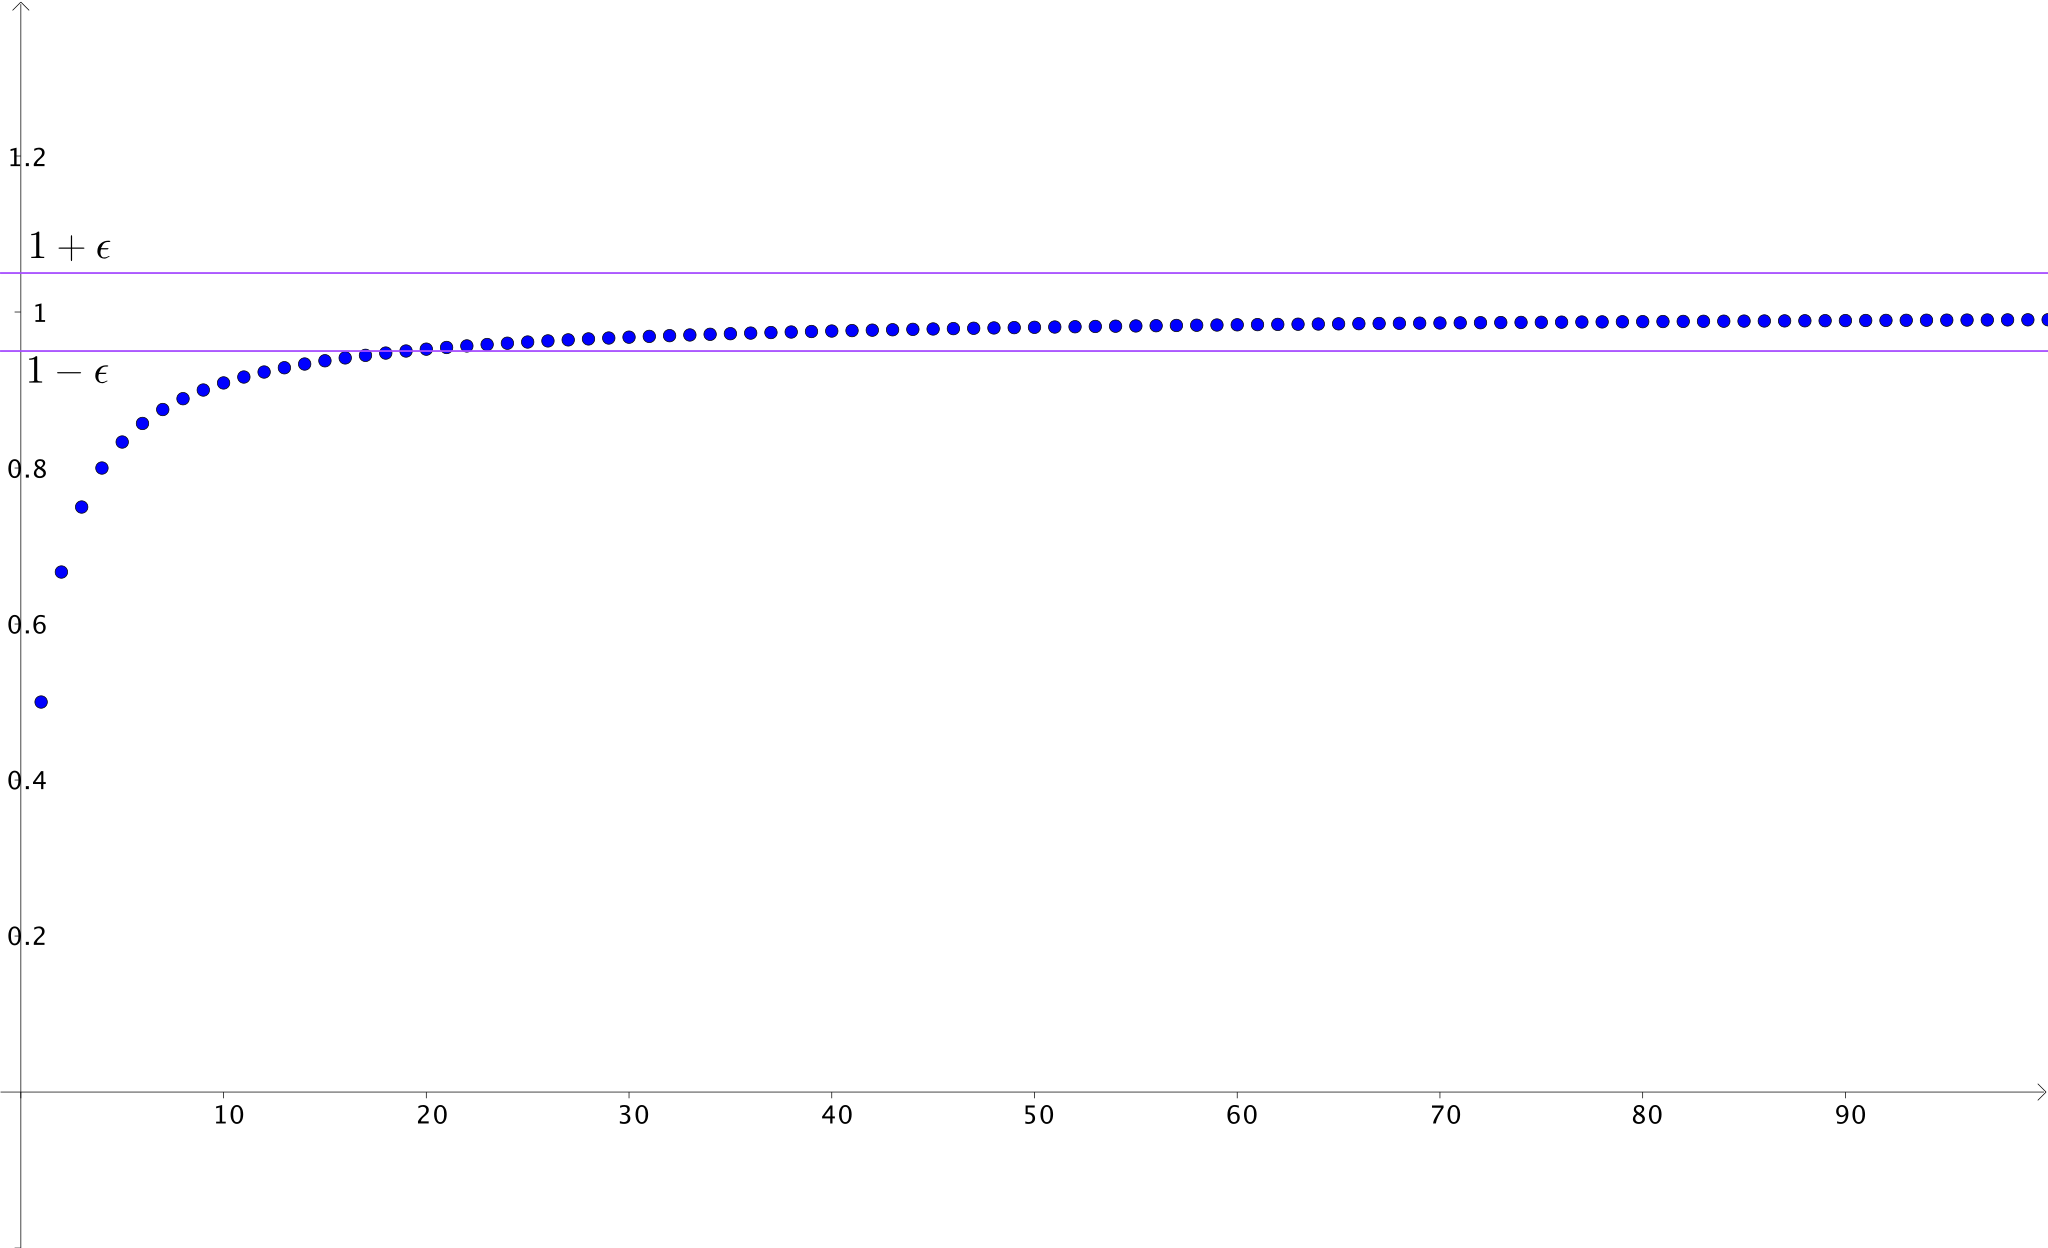
\includegraphics{Sequence_limit}}
\caption{The limit of the sequence $\left(\frac{n}{1+n}\right)$.} 
\label{F:sequence_limit}
\end{center}
\end{figure}
To verify that the limit of the sequence $\left(\frac{n}{1+n}\right)$ is $1$, we start with $\epsilon > 0$. 

\begin{quote} \textbf{Scratch work.} Now we need to find $N$ so that $n \geq N$ implies $\left| \frac{n}{1+n} - 1 \right| < \epsilon$. Just as with our continuity example, this work is not part of the proof, but shows how we go about finding the $N$ we need. To make $\left| \frac{n}{1+n} - 1 \right| < \epsilon$ we need
\begin{align*}
\left| \frac{n}{1+n} - 1 \right| &< \epsilon \\
\left| \frac{n}{1+n} - \frac{1+n}{1+n}  \right| &< \epsilon \\
\left| \frac{-1}{1+n} \right| &< \epsilon \\
1+n &> \frac{1}{\epsilon} \\
n &> \frac{1}{\epsilon} -1.
\end{align*}

Now we use this scratch work to design our proof. 
\end{quote}

Let $N > \frac{1}{\epsilon} -1$ (so that $N$ depends on $\epsilon$). Then for $n \geq N$ we have 
\begin{align*}
n &> N > \frac{1}{\epsilon} -1 \\
1+n &> \frac{1}{\epsilon} \\
|-1| \left| \frac{1}{1+n} \right| &< \epsilon \\
\left| \frac{-1}{1+n} \right| &< \epsilon \\
\left| \frac{n}{1+n} - 1 \right| &< \epsilon \\
\left| \frac{n}{1+n} - \frac{1+n}{1+n}  \right| &< \epsilon.
\end{align*}
So the sequence $\left(\frac{n}{1+n}\right)$ has a limit of $1$.
\end{example}

Definition \ref{def:sequence_limit_real} only applies to sequences of real numbers. Ultimately, we want to phrase the definition in a way that allows us to define limits of sequences in metric spaces and topological spaces. So we have to reformulate the definition in such a way that it does not depend on distances. 

Recall that $| x-y |$ defined a metric $d_E$ on $\R$, that is 
\[d_E(x,y) = | x-y |.\]
So we can rephrase the definition of a limit of a sequence of real numbers as follows.

\begin{definition}[Alternate Definition] A sequence $(a_n)$ of real numbers has a \textbf{limit} $L$ if, given any $\epsilon > 0$ there exists a positive integer $N$ such that 
\[d_E(a_n, L) < \epsilon \ \text{ whenever } \ n \geq N.\]
\end{definition}

Once we have described a limit of a sequence in terms of a metric, then we can extend the idea into any metric space. 

\begin{definition} A \textbf{sequence}\index{sequence in a metric space} in a metric space $(X,d)$ is a function $f: \Z^+ \to X$.  
\end{definition}

If $f$ is a sequence in $X$, we write the sequence defined by $f$ as $(f(n))$, where $n \in \Z^+$. We also use the notation $(a_n)$, when $a_n = f(n)$. As long as $X$ has a metric defined on it, we can then describe the limit of a sequence.

\begin{definition} Let $(X,d)$ be a metric space. A sequence $(a_n)$ in $X$ has a \textbf{limit}\index{limit of a sequence in a metric space} $L \in X$ if, given any $\epsilon > 0$ there exists a positive integer $N$ such that 
\[d(a_n, L) < \epsilon \ \text{ whenever } \ n \geq N.\]
\end{definition}

In other words, a sequence  $(a_n)$ in a metric space $(X,d)$ has a limit $L \in X$ if $\lim d(a_n,L) = 0$ -- or that the sequence $d(a_n,L)$ of real numbers has a limit of $0$. Just as with sequences of real numbers, when a sequence $(a_n)$ has a limit $L$, we say that the sequence $(a_n)$ \emph{converges} to $L$, or that $L$ is a limit of the sequence $(a_n)$. 

\begin{pa} ~
\be
\item Explain why the sequence $\left(\frac{1}{n}\right)$ converges to 0 in $\R$ using the Euclidean metric $d_E$, where 
\[d_E(a,y) = | x-y |.\]

\item Consider the sequence $(a_n) = \left(\left(\frac{1}{n}, \frac{1}{n+1} \right)\right)$ in $(\R^2, d_T)$, where $d_T$ is the taxicab metric
\[d_T((x_1, x_2), (y_1, y_1)) = | x_1-y_1| + | x_2-y_2 |.\]
Does the sequence $(a_n)$ converge? If so, find its limit and prove that your candidate is the limit. If not, explain why.

\item Let $(b_n) = \left((2n, n^2)\right)$ in the metric space $(\R^2, d)$, where $d$ is the discrete metric defined by 
\[d(x,y) = \begin{cases} 0 &\text{if } x=y \\ 1 &\text{if } x \neq y. \end{cases}\]
Does the sequence $(b_n)$ converge? If so, find its limit and prove that your candidate is the limit. If not, explain why.

\ee

\end{pa}


\begin{comment}

\ActivitySolution

\be
\item  Let $a_n = \frac{1}{n}$ for each positive integer $n$. Let $\epsilon > 0$. We will show that there is a positive integer $N$ such that $n \geq N$ implies $d_E(a_n,0) < \epsilon$. Since the set of positive integers is unbounded above, there exists a positive integer $N$ so that $\frac{1}{N} < \epsilon$. Then, if $n \geq N$, it follows that 
\[d_E(a_n,0) = | a_n-0 | = | \frac{1}{n} | \leq \frac{1}{N} < \epsilon.\]
We conclude that $lim \frac{1}{n} = 0$.   

\item  We will show that $\lim a_n = (0,0)$. Let $\epsilon > 0$. Choose $N \in \Z^+$ so that $N > \frac{2}{\epsilon}$. This makes $\frac{1}{N} < \frac{\epsilon}{2}$. Note that $\frac{1}{N+1} < \frac{1}{N} < \frac{\epsilon}{2}$ as well. Now let $n \geq N$. Then 
\begin{align*}
d_T(a_n, (0,0)) &= \left| \frac{1}{n} - 0 \right| + \left| \frac{1}{n+1} - 0 \right| \\
	&= \frac{1}{n} + \frac{1}{n+1} \\
	&\leq \frac{1}{N} + \frac{1}{N+1} \\
	&< \frac{\epsilon}{2} + \frac{\epsilon}{2} \\
	&= \epsilon.
\end{align*}


\item  We claim that the sequence $(b_n)$ does not have a limit. To demonstrate this, we proceed by contradiction and assume that the sequence $(b_n)$ has a limit $b$. So for any $\epsilon > 0$ there exists an integer $N > 0$ so that $n \geq N$ implies $d(b_n,b) < \epsilon$. Let $\epsilon = \frac{1}{2}$. Now $(2n,n^2) \neq (2m,m^2)$ if $m \neq n$ in $\Z$, so all of the entries of the sequence $(b_n)$ are distinct. Now either $b = b_n$ for some $n$ or $b \neq b_n$ for all $n$. In either case there is a large enough $N$ so that $b \neq b_n$ for all $n \geq N$. Then $n \geq N$ implies 
\[d(b_n,b) = 1 > \epsilon.\]
So there cannot be an integer $N > 0$ so that $d(b_n,b) < \epsilon$ for $n \geq N$, no matter what $b$ is, so the sequence $(b_n)$ does not have a limit.

\ee

\end{comment}

\csection{Sequences and Continuity in Metric Spaces}\label{sec_seq_cont_metric}

There are different characterizations of continuity. We have already see the $\epsilon$-$\delta$ definition and a characterization in terms of neighborhoods. In this section we investigate sequences and limits of sequences in metric spaces, and then provide a characterization of continuous functions in terms of sequences. 

\begin{activity} A reasonable question to ask is if a limit of a sequence is unique. We will answer that question in this activity. Let $(X,d)$ be a metric space and $(a_n)$ a sequence in $X$. Assume the sequence $(a_n)$ has a limit in $X$. To show that a limit of the sequence $(a_n)$ is unique, we need to show that if $\lim a_n = a$ and $\lim a_n = a'$ for some $a, a' \in X$, then $a=a'$.

Suppose $\lim a_n = a$ and $\lim a_n = a'$ for some $a, a' \in X$. Without much to go on it might appear that proving $a=a'$ is a difficult task. However, if $d(a,a') < \epsilon$ for any $\epsilon > 0$, then it will have to be the case that $a=a'$. So let $\epsilon > 0$. 

	\ba
	\item Why must there exist a positive integer $N$ so that $d(a_n, a) < \frac{\epsilon}{2}$ for all $n \geq N$?

	\item Why must there exist a positive integer $N'$ so that $d(a_n, a') < \frac{\epsilon}{2}$ for all $n \geq N'$?

	\item Now let $m = \max\{N, N'\}$. What can we say about $d(a_m,a)$ and $d(a_m,a')$? Why?
	
	\item Use the triangle inequality to conclude that $d(a,a') < \epsilon$. What else can we conclude?

	\ea

\end{activity}

\begin{comment}

\ActivitySolution
	\ba
	\item Since $a$ is a limit of $(a_n)$, the definition of a limit of a sequence states that, given $\frac{\epsilon}{2}$ (using $\frac{\epsilon}{2}$ in place of $\epsilon$), there exists a positive integer $N$ so that $d(a_n, a) < \frac{\epsilon}{2}$ for all $n \geq N$.

	\item Since $a'$ is a limit of $(a_n)$, the definition of a limit of a sequence states that, given $\frac{\epsilon}{2}$ (using $\frac{\epsilon}{2}$ in place of $\epsilon$), there exists a positive integer $N'$ so that $d(a_n, a') < \frac{\epsilon}{2}$ for all $n \geq N'$.

	\item Since $m$ is larger than $N$ we know that $d(a_m,a) < \frac{\epsilon}{2}$. Since $m$ is larger than $N'$ we know that $d(a_m,a') < \frac{\epsilon}{2}$. 
		
	\item We now have that
	\[d(a,a') \leq d(a,a_m) + d(a_m,a') < \frac{\epsilon}{2} + \frac{\epsilon}{2} = \epsilon.\]
	From this we can conclude that $a = a'$. 
	
	\ea

\end{comment}

Continuity can also be described in terms of sequences. The basic idea is this. Suppose that $f : \R \to \R$ is continuous at a point $a$. This means that $f$ has a limit (as a continuous function) at $a$. So if we were to take any sequence $(a_n)$ that converges to $a$, then the continuity of $f$ implies that $f(a) = f(\lim a_n) = \lim f(a_n)$. That this is both a necessary condition and a sufficient condition for continuity is given in the next theorem.

\begin{theorem} \label{thm:seq_continuity}  Let $(X,d_X)$ and $(Y,d_Y)$ be metric spaces, and let $a \in X$. A function $f:X \to Y$ is continuous at $a$ if and only if $\lim f(a_n) = f(a)$ for any sequence $(a_n)$ in $X$ that converges to $a$. 
\end{theorem}

\begin{proof} Let $(X,d_X)$ and $(Y,d_Y)$ be metric spaces, let $a \in X$, and let $f: X \to Y$ be a function. Assume that $f$ is continuous at $a$. We will show that $\lim f(a_n) = f(a)$ for any sequence $(a_n)$ in $X$ that converges to $a$. Let $(a_n)$ be a sequence in $X$ that converges to $a$ (we know such a sequence exists, namely the sequence $(a)$). To verify that $\lim f(a_n) = a$, let $\epsilon > 0$. The fact that $f$ is continuous at $a$ means that there is a $\delta > 0$ so that $d_Y(f(x), f(a)) < \epsilon$ whenever $d_X(x,a) < \delta$. Since $(a_n)$ converges to $a$, we know that there exists a positive integer $N$ such that $d_X(a_n, a) < \delta$ whenever $n \geq N$. This implies that 
\[d_Y(f(a_n), f(a)) < \epsilon \ \text{ whenever } \ n \geq N.\]
We conclude that if $f$ is continuous at $a$, then $\lim f(a_n) = f(a)$ for any sequence $(a_n)$ in $X$ that converges to $a$.

The proof of the reverse implication is contained in the next activity.
\end{proof}


\begin{activity} Let $(X,d_X)$ and $(Y,d_Y)$ be metric spaces, let $a \in X$, and let $f: X \to Y$ be a function. We prove the remaining implication of Theorem \ref{thm:seq_continuity}, that $f$ is continuous at $a$ if $\lim f(a_n) = f(a)$ for any sequence $(a_n)$ in $X$ that converges to $a$, in this activity. 
\ba
\item To have an additional assumption with which to work, let us proceed by contradiction and assume that $f$ is not continuous at $a$. Why can we then say that there is an $\epsilon > 0$ so that there is no $\delta > 0$ with the property that $d_X(x,a) < \delta$ implies $d_Y(f(x), f(a)) < \epsilon$?

\item To create a contradiction, we will construct a sequence $(a_n)$ that converges to $a$ while $(f(a_n))$ does not converge to $f(a)$. 
	\begin{enumerate}[i.]
	\item Explain why we can find a positive integer $K$ such that $\frac{1}{K} < \epsilon$.
	
	\item If $k > K$, explain why there is an element $a_k \in B\left(a, \frac{1}{k}\right)$ so that $d_Y(f(a_k), f(a)) \geq \epsilon$.

\item For $k \leq K$, let $a_k$ be any element in $B\left(a, \frac{1}{k}\right)$. Explain why $a$ is a limit of $(a_n)$. 

\item Explain why $f(a)$ is not a limit of the sequence $(f(a_n))$. What conclusion can we draw, and why? 

	\end{enumerate}
\ea

\end{activity}

\begin{comment}

\ActivitySolution

\ba
\item Since $f$ is not continuous at $a$, we negate the definition of continuity, negating universal and existential quantifiers. This tells us that exists an $\epsilon > 0$ such that there is no $\delta > 0$ with the property that $d_X(x,a) < \delta$ implies $d_Y(f(x), f(a)) < \epsilon$.

\item 
	\begin{enumerate}[i.]
	\item The sequence $\frac{1}{k}$ of real numbers converges to $0$, so we can make $\frac{1}{k}$ as close to $0$ as we like. That means we can make $\frac{1}{k}$ less than $\epsilon$ if $k$ is large enough. So there is some positive integer $K$ such that $\frac{1}{K} < \epsilon$. 
	
	\item From part (a), for each $k > K$ there is no $\delta$  with the property that $d_X(x,a) < \delta$ implies $d_Y(f(x), f(a)) < \epsilon$. Thus, there must be some element $a_k$ with $d_X(a_k,a) < \frac{1}{k}$ and $d_Y(f(a_k),f(a)) > \epsilon$. Since $d_X(a_k,a) < \frac{1}{k}$, we know that $a_k \in B\left(a, \frac{1}{k}\right)$. 
	
	\item Choosing any $a_k \in B\left(a, \frac{1}{k}\right)$ when $k \leq K$ gives us a sequence $(a_n)$. We now show that $a$ is the limit of $(a_n)$. Let $\alpha > 0$. Let $N$ be a positive integer such that $\frac{1}{N} < \alpha$. If $n \geq N$, since $a_n \in B\left(a, \frac{1}{n}\right)$, we see that 
	\[d_X(a_n,a) < \frac{1}{n} < \frac{1}{N} < \alpha.\]
	Therefore, the sequence $(a_n)$ has a limit of $a$. 
	
	\item  Now we demonstrate that $(f(a_n))$ does not have $f(a)$ as a limit. Using $\epsilon$ as given, note that $n > K$ implies that $d_Y(f(a_k), f(a)) \geq \epsilon$. We can always choose $n$ larger enough so that $\frac{1}{n} < \delta$ for any given $\delta > 0$. So there can be no $\delta$ such that $d(x,a) < \delta$ implies $d_Y(f(a_k),f(a)) < \epsilon$. 

	\item Assuming that $f$ is not continuous at $a$ led to the construction of a sequence $(a_n)$ with limit $a$, but $\lim f(a_n) \neq f(a)$. This contradicts our hypothesis. We must therefore conclude that $f$ is continuous at $a$. 

	\end{enumerate}
\ea


\end{comment}

One way that Theorem \ref{thm:seq_continuity} is often used is illustrated in the next activity. 

\begin{activity} \label{act:sequence_continuity} Let $f$ be the function from $\R$ to $\R$, both with the Euclidean metric, defined by 
\[f(x) = \begin{cases} \sin\left(\frac{1}{x}\right) &\text{ if } x \neq 0 \\ 0 &\text{ if } x = 0. \end{cases}\]
We consider the $f$ continuity of $f$ at $0$ in this activity.

	\ba
	\item Draw a graph of $f$ on some small interval centered at $0$. Based on the  graph, do you think $f$ has a limit at $0$? Explain. (There is no right answer here, just your intuition based on the graph.)
	
	\item At which inputs is $f(x)=1$? 
	
	\item Use the result of (b) to find a sequence $(a_n)$ that converges to $0$ for which $f(a_n) = 1$ for every $n$.
	
	\item What does the result of (c) tell us about the continuity of $f$ at $0$? 
	

	\ea

\end{activity}

\begin{comment}

\ActivitySolution

\ba

\item A graph of $f$ on the interval $[-1,1]$ is shown in Figure \ref{F:top_sine}. Based on the appearance of the graph, it looks as though the graph oscillates back and forth infinitely often between $-1$ and $1$ as $x$ gets close to $0$. So we don't expect the function $f$ to have a limit at $0$.  
\begin{figure}[h]
\begin{center}
\resizebox{!}{2.0in}{\includegraphics{topologist_sine}}
\caption{A graph of $f(x)$.} 
\label{F:top_sine}
\end{center}
\end{figure}

\item We will have $f(x) = 1$ when $\sin\left(\frac{1}{x}\right) = 1$. This happens when $\frac{1}{x} = \frac{\pi}{2} + k \pi$ for any integer $k$, or when 
\[x = \frac{1}{\frac{\pi}{2} + k \pi}.\]

\item Let $a_n = \frac{1}{\frac{\pi}{2} + n \pi}$. As $n$ goes to infinity, $a_n$ converges to $0$. But $f(a_n) = 1$ for every $n$. This means that if $f$ has a limit at $0$, that limit has to be $1$. But $f(0) = 0$, so $f$ is not continuous at $0$. 

\ea

\end{comment}

While it can sometimes be difficult to prove a fact about all sequences that converge to a point, Activity \ref{act:sequence_continuity} shows that we can use Theorem \ref{thm:seq_continuity} to prove that a function $f$ is not continuous at an input $a$ be finding just one sequence $(a_n)$ that converges to $a$ for which $\lim f(a_n) \neq f(a)$. We conclude this section with one final note. 

\noindent IMPORTANT NOTE: Theorem \ref{thm:seq_continuity} tells us that if $f : X \to Y$ is a continuous function, then $f$ commutes with limits. That is, if $(a_n)$ is a sequence in $X$ that converges to $a \in X$, then 
\[f(a) = f(\lim a_n) = \lim f(a_n).\]


 \csection{Summary}\label{sec_seq_summ}
Important ideas that we discussed in this section include the following.
\begin{itemize}
\item A sequence in a metric space $X$ is a function $f : \Z^+ \to X$.
\item  A sequence $(a_n)$ in a metric space $(X,d)$ has a limit $L$ in $X$ if, given any $\epsilon > 0$ there exists a positive integer $N$ such that $d(a_n,L) < \epsilon$ whenever $n \geq N$.
\item Let $f$ be a function from a metric space $(X,d_X)$ to m metric space $(Y,d_Y)$. Then $f$ is continuous at $a \in X$ if and only if $\lim f(a_n) = f(a)$ for any sequence $(a_n)$ in $X$ that converges to $a$.
\end{itemize}

\csection{Exercises}\label{sec_seq_exer}

\be

\item Determine, with proof, the convergence or divergence of each of the following sequences in the indicated metric spaces.

\ba

\item $a_n = 1+\frac{1}{n}$ in $(\R, d_E)$

\item $a_n = (2,n)$ in $(\R^2, d_M)$

\item $a_n$ is the function defined by 
\[a_n(x) = \frac{1}{n}x\]
where $X$ is the set of real valued functions on the interval $[0,1]$ and the metric $d$ is defined by 
\[d(f,g) = \sup\{|f(x)-g(x)| \mid x \in [0,1]\}.\]
(See Exercise \ref{ex:GLB_function_sup_metric} on page \pageref{ex:GLB_function_sup_metric}.)


\ea

\begin{comment}

\ExerciseSolution 

\ba

\item We prove that $(a_n)$ converges to $1$. Let $\epsilon$ be a positive real number. We know there is an $N \in \Z^+$ such that $\frac{1}{N} < \epsilon$. Then if $n \geq N$, 
\[|a_n - 1| = \left|\frac{1}{n}\right| < \frac{1}{N} < \epsilon.\]
Therefore, $\lim a_n = 1$. 

\item We prove that $(a_n)$ has no limit. Let $a = (u,v)$ be a point in $\R^2$ and let $\epsilon$ be a positive real number.  We know that 
\[d_M(a_n,a) = \max\{|2-u|, |n-v|\}.\]
By the Archimedean property, there is $M \in \Z^+$ such that $M - v \geq \epsilon$. So if $n \geq M$ we have 
\[d_M(a_n,a) = \max\{|2-u|, |n-v|\} \geq |n-v| > M-v \geq \epsilon.\] 
So there can be no $N \in \Z^+$ with $d_M(a_n,a) < \epsilon$ whenever $n \geq N$. We conclude that the sequence $(a_n)$ has no limit. 

\item We prove that the sequence $(a_n)$ converges to the constant function $a$ defined by $a(x) = 0$ for all $x \in [0,1]$. Notice that $a_n(x)$ is the linear function connecting the points $(0,0)$ and $\left(1,\frac{1}{n}\right)$. So 
\[d(a_n,a) = \sup\{|a_n(x)-a(x)| \mid x \in [0,1]\} = \left(\frac{1}{n}-0\right| = \frac{1}{n}.\]
Let $\epsilon > 0$. By the Archimedean property, there is an $N \in \Z^+$ such that $N > \frac{1}{\epsilon}$. Then for $n \geq N$ we have 
\[d(a_n,a) = \frac{1}{n} \leq \frac{1}{N} < \epsilon.\]

\ea

\end{comment}


\item Let $A$ be a subset of $\R$.

\ba

\item Show that if $A$ is bounded above, then there is a sequence $(a_n)$ in $A$ such that $\lim a_n = \sup(A)$. 

\item Show that if $A$ is bounded below, then there is a sequence $(a_n)$ in $A$ such that $\lim a_n = \inf(A)$. 

\item Are the limits from (a) or (b) necessarily in $A$? Explain.
\ea

\begin{comment}

\ExerciseSolution

\ba

\item Assume that $A$ is bounded above so that $s = \sup(A)$ exists. Let $n \in \Z^+$. Since $s-\frac{1}{n} < s$, we know that $s-\frac{1}{n}$ is not an upper bound for $A$. So there exists $a_n \in A$ such that $s-\frac{1}{n} < a_n \leq s$. Given any $\epsilon > 0$, there exists $N \in \Z^+$ such that $\frac{1}{N} < \epsilon$. So if $n \geq N$, then $|a_n - s| < \frac{1}{n} < \frac{1}{N} < \epsilon$. We conclude that $\lim a_n = s$. 

\item Assume that $A$ is bounded above so that $t = \inf(A)$ exists. Let $n \in \Z^+$. Since $t+\frac{1}{n} < t$, we know that $t+\frac{1}{n}$ is not a lower bound for $A$. So there exists $a_n \in A$ such that $t \leq a_n < t+\frac{1}{n}$. Given any $\epsilon > 0$, there exists $N \in \Z^+$ such that $\frac{1}{N} < \epsilon$. So if $n \geq N$, then $|a_n - t| < \frac{1}{n} < \frac{1}{N} < \epsilon$. We conclude that $\lim a_n = t$. 

\item Let $A$ be the open interval $(0,1)$ in $\R$ with the Euclidean metric.  Then $\sup(A) = 1$ and $\inf(A) = 0$. So neither limit needs to be in $A$.  
\ea

\end{comment}

\item Let $(X,d)$ be a metric space, let $x \in X$, and let $A$ be a nonempty subset of $X$. Recall that the distance from $x$ to $A$ is 
\[d(x,A) = \inf \{d(x,a) \mid a \in A.\]
In this exercise we see how we can view the distance between a point and a set in terms of sequences. Let $m = d(x,A)$. We will show that there must be a sequence $(a_n)$ in $A$ so that $d(x,A) = \lim d(x,a_n)$. 
\ba
\item For each $n \in \Z^+$, let $B_n = B\left(x;m+\frac{1}{n}\right)$. Why must $B_n \cap A \neq \emptyset$ for each $n \in \Z^+$? 

\item Let $a_n \in B_n \cap A$ for each $n$. What property does this sequence have? Explain how we have just proved the following theorem.

\begin{theorem} Let $(X,d)$ be a metric space, let $x \in X$, and let $A$ be a nonempty subset of $X$. Then there exists a sequence $(a_n)$ in $A$ such that 
\[\lim d(x,a_n) = d(x,A).\]
\end{theorem}

\ea


\begin{comment}

\ExerciseSolution

\ba
\item Suppose to the contrary that there is an $n \in \Z^+$ such that $B_n \cap A = \emptyset$. Then there is no element $c \in A$ such that $d(x,c) < m + \frac{1}{n}$. This makes $m + \frac{1}{n}$ a lower bound for $\{d(x,a) \mid a \in A\}$ greater than the greatest lower bound of $\{d(x,a) \mid a \in A\}$. Since this cannot happen, we conclude that $B_n \cap A \neq \emptyset$ for every $n \in \Z^+$. 

\item We have
\[\lim d(x,a_n) \leq \lim \left(m+\frac{1}{n}\right) = m.\]
So we have found a sequence $(a_n)$ in $A$ satisfying $\lim d(x,a_n) = d(x,A)$.

\ea

\end{comment}

\item ~
	\ba
	\item Let $(Y,d')$ be a subspace of $(X,d)$. Let $a_1$, $a_2$, $\ldots$ be a sequence of points in $Y$ and let $a \in Y$. Prove that if $\lim_n a_n = a$ in $(Y,d')$, then $\lim_n a_n = a$ in $(X,d)$. 

	\item Show that the converse of part (a) is false by considering the subspace $(\Q, d_{\Q})$ (the rational numbers) of $(R,d)$. Let $a_1$, $a_2$, $\ldots$ be a sequence of rational numbers such that $\lim_n a_n = \sqrt{2}$. Prove that , given $\epsilon > 0$, there is a positive integer $N$ such that for $n, m > N$, $|a_n - a_m | < \epsilon$. Does the sequence  $a_1$, $a_2$, $\ldots$ converge when considered to be a sequence of points in $\Q$?  

	\ea

\begin{comment}

\ExerciseSolution 
\ba
\item Let $(Y,d')$ be a subspace of $(X,d)$. Let $a_1$, $a_2$, $\ldots$ be a sequence of points in $Y$ and assume $\lim_n a_n = a$ for some $a \in Y$. Let $\epsilon > 0$. Then there exists an $N \in \Z^+$ so that $d'(a_n,a) < \epsilon$ whenever $n \geq N$. But $d'(a_n,a) = d(a_n,a)$, so $d(a_n,a) < \epsilon$ whenever $n \geq N$. This implies that $\lim a_n = a$ in $X$. 

\item Here we assume $d = d_E$ in $\R$ and that $d_{\Q}$ is the restriction of $d$ to $\Q$. Let $\epsilon > 0$. Since $\lim a_n = \sqrt{2}$, there exists $N \in \Z^+$ so that $n \geq N$ implies $| a_n - \sqrt{2} | < \frac{\epsilon}{2}$. Now let $n, m > N$. The triangle inequality then gives us \[| a_n - a_m | \leq | a_n - \sqrt(2)| + | \sqrt{2} - a_m | < \frac{\epsilon}{2} + \frac{\epsilon}{2} = \epsilon.\]

Now we will show that the sequence $(a_n)$ does not converge as a sequence in $\Q$. Assume to the contrary that the sequence $(a_n)$ does converge as a sequence in $\Q$. The uniqueness of limits then implies that $\sqrt{2}$ is a rational number. That means that $\sqrt{2} = \frac{p}{q}$ for some relatively prime positive integers $p$ and $q$. This implies that $q\sqrt{2} = p$ or $2q^2 = p^2$. The fact that $2$ divides $p^2$ means that $p$ must be even. So $p = 2r$ for some positive integer $r$. It follows that 
\[2q^2 = (2r)^2 = 4r^2.\]
But then $q^2 = 2r^2$ and $2$ divides $q$. This contradicts the fact that $p$ and $q$ are relatively prime. So $\sqrt{2}$ is not a rational number and the sequence $(a_n)$ does not converge as a sequence in $\Q$.  

\ea

\end{comment}

\item \label{ex:limit_properties} In this exercise we prove some standard results about limits of sequences from calculus. Let $(a_n)$ and $(b_n)$ be convergent sequences in a metric space $(\R,d_E)$. 

\ba

\item Show that $\lim ka_n = k \lim a_n$ for any real number $k$.

\item Show that $\lim (a_n + b_n) = \lim a_n + \lim b_n$. 

\item Show that the sequence $(a_n)$ is bounded. That is, show that there is a positive real number $M$ such that $|a_n| \leq M$ for all $n \in \Z^+$. 

\item Show that $\lim a_nb_n = \lim a_n \ \lim b_n$. 

\item If $b_n \neq 0$ for every $n$ and $\lim b_n \neq 0$, show that $\lim \frac{a_n}{b_n} = \frac{\lim a_n}{\lim b_n}$. 

\ea

\begin{comment}

\ExerciseSolution

\ba

\item Let $a = \lim a_n$, let $k \in \R$, and let $\epsilon$ be a positive real number. If $k = 0$, then 
\[\lim ka_n = \lim 0 = 0 = 0(a) = 0\lim a_n.\]
So suppose $k \neq 0$. Let $N \in \Z^+$ such that $d(a_n, a) < \frac{\epsilon}{|k|}$ if $n \geq N$. So if $n \geq N$, then 
\[d_E(ka_n, ka) = |k|d_E(a_n,a) < |k| \frac{\epsilon}{|k|} = \epsilon.\]
So $\lim ka_n = ka$. 

\item Let $a = \lim a_n$, $b = \lim b_n$, and let $\epsilon$ be a positive real number. There exists $N_1 \in \Z^+$ such that $d_E(a_n,a) < \frac{\epsilon}{2}$ whenever $n \geq N_1$, and there exists $N_2 \in \Z^+$ such that $d_E(b_n,b) < \frac{\epsilon}{2}$ whenever $n \geq N_2$. Let $N = \max\{N_1, N_2\}$. Then if $n \geq N$ we have 
\begin{align*}
d_E(a_n+b_n, a+b) &= |(a_n+b_n) - (a+b)| \\
	&= |(a_n-a) + (b_n-b)| \\
	&\leq |a_n-a| + |b_n-b| \\
	&< \frac{\epsilon}{2} + \frac{\epsilon}{2} \\
	&= \epsilon.
\end{align*}
Therefore,  $\lim (a_n + b_n) = \lim a_n + \lim b_n$. 

\item Let $a = \lim a_n$. There exists $N \in \Z^+$ such that $d_E(a_n,a) < 1$ whenever $n \geq N$. Thus, if $n \geq N$, we have $|a_n-a| < 1$ or $a-1 < a_n < a+1$. So $|a_n| < K$ for $n \geq N$, where $K = \max\{|a-1|, |a+1|\}$. Let $M = \max\{|a_1|, |a_2|, \ldots, |a_{N-1}|, K\}$. Then $|a_n| \leq M$ for all $n \in \Z^+$. 
 
\item Let $a = \lim a_n$, $b = \lim b_n$, and let $\epsilon$ be a positive real number. The sequence $(b_n)$ is bounded by the previous part of this problem, so let $M$ be an upper bound for $\{|b_n| \mid n \in \Z^+\}$. There exists $N_1 \in \Z^+$ such that $d_E(a_n,a) < \frac{\epsilon}{2(K+1)}$ whenever $n \geq N_1$, and there exists $N_2 \in \Z^+$ such that $d_E(b_n,b) < \frac{\epsilon}{2(|a|+1)}$ whenever $n \geq N_2$. Let $N = \max\{N_1, N_2\}$. Then if $n \geq N$ we have 
\begin{align*}
d_E(a_nb_n, ab) &= |a_nb_n - ab| \\
	&= |a_nb_n - b_na + b_na- ab| \\
	&= |b_n(a_n-a) + a(b_n-b)| \\
	&\leq |b_n| |a_n-a| + |a| |b_n-b| \\
	&< K\left(\frac{\epsilon}{2(K+1)} + |a|\frac{\epsilon}{2(|a|+1)}\right) \\
	&< \frac{\epsilon}{2} + \frac{\epsilon}{2} \\
	&= \epsilon.
\end{align*}
Therefore,  $\lim (a_nb_n) = \lim a_n \ \lim b_n$. 


\item Let $b = \lim b_n$. If we show that $\lim \frac{1}{b_n} = \frac{1}{\lim b_n}$, then we can use the result of the previous part because
\[\lim \frac{a_n}{b_n} = \lim a_n \ \lim \frac{1}{b_n} = \lim a_n \ \frac{1}{\lim b_n} = \frac{\lim a_n}{\lim b_n}.\]

One result we will need is that the sequence $(b_n)$ is bounded below by a positive number. There is an $N \in \Z^+$ such that $|b_n - b| < \frac{|b|}{2}$ whenever $n \geq N$. So if $n \geq N$, then $|b_n| > \frac{|b|}{2}$. Let $M = \min\left\{|a_1|, |a_2|, \ldots, |a_{N-1}|, \frac{|b|}{2}\right\}$. Then $|a_n| \geq M$ for all $n \in \Z^+$. 

Now let $\epsilon$ be a positive number. Let $M > 0$ be a lower bound for the sequence $(b_n)$. There exists $N \in \Z^+$ such that $d_E(b_n,b) < \epsilon \ |b| \ M$ whenever $n \geq N$. So if $n \geq N$, then 
\begin{align*}
d_E\left(\frac{1}{b_n}, \frac{1}{b}\right) &= \left| \frac{1}{b_n} - \frac{1}{b} \right| \\
	&= \left| \frac{b-b_n}{bb_n} \right| \\
	&\leq \frac{1}{|bb_n|} \epsilon \ |b| \ M \\
	&= \frac{M}{|b_n|} \epsilon \\
	&< \epsilon.
\end{align*}
So $\lim \frac{1}{b_n} = \frac{1}{\lim b_n}$ as desired.
	

\ea

\end{comment}


\item Let $f$ and $g$ be continuous functions from $\R$ to $\R$, both with the standard Euclidean metric. Define the function $fg$ from $\R$ to $\R$ by 
\[(fg)(x) = f(x)g(x) \text{ for every } x \in \R.\]
	\ba
	\item Prove that $fg$ is a continuous function.
	
	\item Assume that $g(x) \neq 0$ for every $x \in \R$. Define the function $\frac{f}{g}$ from $\R$ to $\R$ by $\frac{f}{g}(x) = \frac{f(x)}{g(x)}$ for every $x \in \R$. Use the definition of continuity to prove that $\frac{f}{g}$ is a continuous function.
	
	\ea
	
\begin{comment}

\ExerciseSolution

\ba
\item Let $a \in \R$. Let $(a_n)$ be a sequence in $\R$ that converges to $a$. Since $f$ and $g$ are continuous at $a$, we know that $\lim f(a_n) = f(a)$ and $\lim g(a_n) = g(a)$. We use the result of Exercise \ref{ex:limit_properties} on the sequences $(f(a_n))$ and $(g(a_n))$. to see that 
\[\lim (fg)(a_n) = \lim f(a_n)g(a_n) = \lim f(a_n) \lim g(a_n) = f(a) g(a).\]
So $fg$ is continuous at $a$. 

\item Similar to part (a) we have 
\[\lim \left(\frac{f}{g}\right)(a_n) = \lim \frac{f(a_n)}{g(a_n)} = \frac{\lim f(a_n)}{ \lim g(a_n)} = \frac{f(a)}{g(a)}.\]
So $\frac{f}{g}$ is continuous at $a$. 

\ea

\end{comment}

\item Let $(c_n) = (a_n,b_n)$ be a sequence in $(\R^2, d_E)$. Show that the sequence $(c_n)$ converges to a point $(a,b)$ if and only if $(a_n)$ converges to $a$ and $(b_n)$ converges to $b$ in $(\R, d_E)$. 

\begin{comment}

\ExerciseSolution First assume that the sequence $(c_n)$ converges to a point $c = (a,b) \in \R^2$. Let $\epsilon$ be a positive number. There exists $N \in \Z^+$ such that $d_E(c_n, c) < \epsilon$ whenever $n \geq N$. So if $n \geq N$ we have
\begin{align*}
d_E(a_n, a) &= |a_n-a| \\
	&\leq \sqrt{ |a_n-a|^2 + |b_n-b|^2} \\
	&= d_E(c_n,c) \\
	&< \epsilon
\end{align*}
and 
\begin{align*}
d_E(b_n, b) &= |b_n-b| \\
	&\leq \sqrt{ |a_n-a|^2 + |b_n-b|^2} \\
	&= d_E(c_n,c) \\
	&< \epsilon.
\end{align*}
We conclude that $(a_n)$ converges to $a$ and $(b_n)$ converges to $b$.

For the converse, we will use the following result:

\begin{lemma} Let $x$ and $y$ be real numbers. Then 
\[\sqrt{x^2+y^2} \leq |x| + |y|.\]
\end{lemma}

\begin{proof} Let $x$ and $y$ be real numbers. Then 
\begin{align*}
x^2 + y^2 &\leq |x|^2 + 2|x| \ |y| + |y|^2 \\
x^2 + y^2 &\leq (|x|+|y|)^2 \\
\sqrt{x^2+y^2} \leq |x| + |y|.
\end{align*}
\end{proof}

Now assume that $(a_n)$ converges to $a$ and $(b_n)$ converges to $b$ in $(\R, d_E)$. Let $c = (a,b)$ and let $\epsilon$ be a positive real number. There exists $N_1 \in \Z^+$ such that $d_E(a_n,a) < \frac{\epsilon}{2} $ whenever $n \geq N_1$ and there exists $N_2 \in \Z^+$ such that $d_E(b_n,b) < \frac{\epsilon}{2} $ whenever $n \geq N_2$. Let $N = \max\{N_1, N_2\}$. Then, using the lemma, if $n \geq N$ we have
\begin{align*}
d_E(c_n,c) &= \sqrt{ |a_n-a|^2 + |b_n-b|^2} \\
	&\leq |a_n-a| + |b_n-b| \\
	&= d_E(a_n,a) + d_E(b_n,b) \\
	&< \frac{\epsilon}{2} + \frac{\epsilon}{2} \\
	&= \epsilon.
\end{align*}
We conclude that $(c_n)$ converges to $c$ in $(\R^2, d_E)$. 

\end{comment}

\item Define $f : (\R,d_E) \to (\R,d_E)$ by 
\[f(x) = \begin{cases} 0 &\text{ if } x \text{ is irrational} \\ x &\text{ if } x \text{ is rational.} \end{cases}\]

\ba

\item Show that $f$ is continuous at exactly one point. Assume that both copies of $\R$ are given the Euclidean topology.

\item Modify the function $f$ to construct a new function $g: \R \to \R$ such that $g$ is continuous at exactly the numbers $0$ and $1$. Prove your result. Can you see how to extend this to construct a function $h: \R \to \R$ that is continuous at any given finite number of points? 

\ea

\begin{comment}

\ExerciseSolution 

\ba

\item First we demonstrate that $f$ is not continuous at every nonzero input. Suppose $a \neq 0$. Every ball centered at $a$ contains a rational number and an irrational number. So for each $n \in \Z^+$, there is a rational number $r_n$ and an irrational number $i_n$ in $B\left(a,\frac{1}{n}\right)$. But then $r_n \to a$ and $i_n \to a$. If $f$ were continuous at $a$, then $f(r_n) \to f(a)$ and $f(i_n) \to f(a)$. But $f(r_n) = r_n \to a$ while $f(i_n) = 0 \to 0 \neq a$. Thus, $f$ is not continuous at $a$. 

Now we demonstrate that $f$ is continuous at $0$. Let $(s_n)$ be a sequence of real numbers with $s_n \to 0$.  Note that $|f(s_n)| \leq |s_n|$, so the fact that $s_n \to 0$ implies that $f(s_n) \to 0$. Therefore, $f$ is continuous at $0$.

\item Define $g: \R \to \R$ by 
\[g(x) = \begin{cases} 0 &\text{ if } x \text{ is irrational} \\ x(x-1) &\text{ if } x \text{ is rational.} \end{cases}\]

First we demonstrate that $g$ is not continuous at every input except $0$ and $1$. Suppose $a \neq 0$ and $a \neq 1$. Every ball centered at $a$ contains a rational number and an irrational number. So for each $n \in \Z^+$, there is a rational number $r_n$ and an irrational number $i_n$ in $B\left(a,\frac{1}{n}\right)$. But then $r_n \to a$ and $i_n \to a$. If $f$ were continuous at $a$, then $f(r_n) \to f(a)$ and $f(i_n) \to f(a)$. But $f(r_n) = r_n(r_n-1) \to a(a-1) \neq 0$ while $f(i_n) = 0 \to 0$. Thus, $f$ is not continuous at $a$. 

Now we demonstrate that $f$ is continuous at $0$ and at $1$. Let $(s_n)$ be a sequence of real numbers with $s_n \to 0$.  Note that $|f(s_n)| \leq |s_n| \ |s_n-1|$, so the fact that $s_n \to 0$ implies that $f(s_n) \to 0 = f(0)$. Therefore, $f$ is continuous at $0$. Now let $(t_n)$ be a sequence of real numbers with $t_n \to 1$.  Note that $|f(t_n)| \leq |t_n| \ |t_n-1|$, so the fact that $t_n \to 1$ implies that $f(t_n) \to 0 = f(1)$. Therefore, $f$ is continuous at $1$.

In general, if $p(x)$ is a real valued polynomial function with zeros at $k$ distinct points, then the function $h: \R \to \R$ defined by 
\[h(x) = \begin{cases} 0 &\text{ if } x \text{ is irrational} \\ p(x) &\text{ if } x \text{ is rational} \end{cases}\]
will be continuous at exactly those zeros of $p(x)$. 

\ea

\end{comment}

\item Let $X$ be the set of real valued functions on the interval $[0,1]$ and let $d$ be the metric on $X$ defined by 
\[d(f,g) = \sup\{|f(x)-g(x)| \mid x \in [0,1]\}.\]
(See Exercise \ref{ex:GLB_function_sup_metric} on page \pageref{ex:GLB_function_sup_metric}.)

There is a difference between the point-wise convergence of a sequence of functions and convergence in the metric space $(X,d)$ that we explore in this exercise. For each $n \in \Z^+$, define $f_n :[0,1] \to \R$ by $f_n(x) = x^n$. 

\ba

\item Let $0 \leq a < 1$. Show that the sequence $(a_n)$ where $a_n = a^n$ converges to $0$ in $(\R, d_E)$. 

\item Since the sequence $(1)$ converges to $1$, if we look at the behavior at each point, we might think that the sequence $(f_n)$ converges to the function $f$ defined by 
\begin{equation} \label{eq:0_1_function}
f(x) = \begin{cases} 0 &\text{ if } x \neq 1 \\ 1 &\text{ if } x=1. \end{cases}
\end{equation}
Determine if the sequence $(f_n)$ converges to $(f)$ in the metric space $(X,d)$.

\item Suppose now we consider the sequence $(f_n)$ as a sequence of functions in $C[0,1]$, the space of continuous functions from $\R$ to $\R$, using the metric
\[d(f,g) = \int_0^1 |f(x) - g(x)| \,dx.\]
(Refer to Activity \ref{act:MS_metrics}.) The function in (\ref{eq:0_1_function}) is not a continuous function, so can't be a limit of the sequence $(f_n)$ in $C[01]$. Determine if the sequence $(f_n)$ has a limit in $C[0,1]$. If so, what is the limit? If not, verify that the sequence has no limit. 

\ea

\begin{comment}

\ExerciseSolution
\ba

\item Let $\epsilon$ be a positive number. We can assume that $\epsilon$ is also less than $1$. Note that $\ln(\epsilon) < 0$ and $\ln(a) < 0$. Let $N \in \Z^+$ such that $N > \frac{\ln(\epsilon)}{\ln(a)}$. Then if $n \geq N$ we have 
\begin{align*}
n &> \frac{\ln(\epsilon)}{\ln(a)} \\
n \ln(a) &< \ln(\epsilon) \\
\ln\left(a^n\right) &< \ln(\epsilon) \\
a^n &< \epsilon \\
\left|a^n - 0\right| &< \epsilon.
\end{align*}
So the sequence $\left(a^n\right)$ converges to $0$ for any $0 \leq a < 1$. 

\item We will show that the sequence $(f_n)$ does not converge to $f$. Since $x^n$ is an increasing function of $x$, it follows that 
\[\sup\{\left|x^n-0\right| \mid 0 \leq x < 1\} = 1.\]
So there is no way that $d(f_n,f)$ can be less than $\epsilon$ if $\epsilon < 1$. 

\item We will how that the sequence $(f_n)$ converges to the $0$ function in $C[0,1]$. Note that 
\[d(f_n,0) = \int_0^1 |x^n - 0| \, dx = \frac{x^{n+1}{n+1}}\biggm|_0^1 = \frac{1}{n+1}.\]
As $n$ goes to infinity, $\frac{1}{n+1}$ converges to $0$. So $\lim (f_n)$ is the zero function. 

\ea

\end{comment}

\item For each of the following, answer true if the statement is always true. If the statement is only sometimes true or never true, answer false and provide a concrete example to illustrate that the statement is false. If a statement is true, explain why.  

	\ba
	\item If $(a_n)$ is a sequence in $(\R, d_E)$ with $a_{n+1} < a_n$ for each $n \in \Z^+$ and the set $\{a_n\}$ is bounded below, then $\inf \{a_n \mid n \in \Z^+\}$ is the limit of the sequence $(a_n)$. 
	
	\item Let $X$ be a metric space and $A$ a nonempty subset of $X$. If $a \in X$ and if $B(a,r)$ in $X$ contains a point of $A$ for every $r > 0$, then there is a sequence in $A$ that converges to $a$. 
	
	\item Let $R$ be a nonempty subset of $\R$ that is bounded above and below. If $S$ is a nonempty subset of $\R$ and $x \leq y$ for all $x \in S$ and for all $y \in R$, then $\sup(S) \leq \inf(R)$. 
	
	\item The sequence $\left(\frac{1}{n}\right)$ converges to $0$ in the metric space $Q$ of all rational numbers in reduced form with metric $d$ defined by
\[d\left(\frac{a}{b}, \frac{r}{s}\right) = \max\{| a-r |, | b-s |\}.\]
(See Exercise \ref{ex:MS_Q_metric} on page \pageref{ex:MS_Q_metric} .)

	\item The only convergent sequences in a metric space $(X,d)$ with discrete metric $d$ are the sequences that are eventually constant. (A sequence $(a_n)$ in a metric space $X$ is eventually constant if there is an element $a \in X$ and an $N \in \Z^+$ such that $a_n = a$ for all $n \geq N$.) 
	
	\ea

\begin{comment}

\ExerciseSolution

\ba

\item This statement is true. To formally verify it, let $a = \inf \{a_n \mid n \in \Z^+\}$. Let $\epsilon > 0$ be given. Since $a+\epsilon$ cannot be a lower bound for $\{a_n\}$, there must be an element $a_N$ in $\{a_n\}$ such that $d_E(a,a_N) < \epsilon$. The fact that $\{a_n\}$ is decreasing means that $d_E(a,a_k) < \epsilon$ whenever $k \geq N$. We conclude that $a \lim a_n$. 
	
	\item This statement is true. To formally verify it, let $n \in \Z^+$. Then there exists $a_n \in A$ with $d(a,a_n) < \frac{1}{n}$. We demonstrate that the sequence $(a_n)$ converges to $a$. Let $\epsilon > 0$ be given. Then let $N \in \Z^+$ such that $N > \frac{1}{\epsilon}$. If $n \geq N$, then $d_E(a_n,a) < \frac{1}{n} < \frac{1}{N} < \epsilon$. 

	\item  This statement is true. Since $R$ is bounded above, $\sup(R)$ exists. The fact that $x \leq y$ for all $x \in S$ and all $y \in R$ means that $S$ is bounded above by $\sup(R)$. Thus, $\sup(S)$ exists. Suppose to the contrary that $\sup(S) > \inf(R)$ and let $\epsilon = \sup(S) - \inf(R)$. Let $(s_n)$ be a sequence in $S$ that converges to $\sup(S)$ and let $(r_n)$ be a sequence in $R$ that converges to $\inf(R)$. There exists $N_1 \in \Z^+$ such that $n \geq N_1$ implies $|s_n - \sup(S)| < \frac{\epsilon}{2}$.  It follows that $s_N > \sup(S) - \epsilon = \inf(R)$. But $s_N < y$ for every $y \in R$, so $s_N$ is a larger lower bound for $R$ than $\inf(R)$, which is impossible. 

	\item This statement is false. If $r > 0$, then $B(0,r)$ in $Q$ is the set of rational numbers $\frac{u}{v}$ in reduced form with 
	\[d\left(\frac{0}{1}, \frac{u}{v}\right) = \max\{|u|, |v-1|\} < r.\]
	But $u$ and $v$ are integers, so there are only finitely many elements of $Q$ that are in $B(0,r)$. So given any $\epsilon > 0$ there can be no $N \in \Z^+$ such that $n \geq N$ implies $d\left(0, \frac{1}{n}\right) < \epsilon$.
	
	\item This statement is true. Let $(a_n)$ be a sequence in a metric space $(X,d)$ that converges to an element $a \in X$, where $d$ is the discrete metric. Then given any $0 < \epsilon < 1$ there is an $N \in \Z^+$ such that $d(a_n,a) < \epsilon$ whenever $n \geq N$. But the only element in $B(a,\epsilon)$ is $a$, so $a_n = a$ for all $n \geq N$.  
	 
\ea




\end{comment}

\ee

  %9
\achapter{10}{Closed Sets in Metric Spaces}\label{sec:closed_sets}

\vspace*{-17 pt}
\framebox{
\parbox{\dimexpr\linewidth-3\fboxsep-3\fboxrule}
{\begin{fqs}
\item What are boundary points, limit points, and isolated points of a set in a metric space? How are they related and how are they different?
\item What does it mean for a set to be closed in a metric space?
\item What important properties do closed sets have in relation to unions and intersections?
\item How can we use closed sets to determine the continuity of a function?
\item How are limit points related to sequences?
\item How are boundary points related to sequences?
\item What is the boundary of a set in a metric space?
\item How are limit points and boundary points related to closed sets?
\item What is the closure of a set in a metric space?
\item How are closed sets related to sequences?
\end{fqs}}}

\vspace*{13 pt}

\csection{Introduction}
Once we have defined open sets in metric spaces, it is natural to ask if there are closed sets. Recall that closed intervals are important in calculus because every continuous function on a closed interval attains an absolute maximum and absolute minimum value on that interval. If we have closed sets in metric spaces, we might consider if there is some result that is similar to this for continuous functions on closed sets. In this section we introduce the idea of closed sets in metric spaces and discover a few of their properties. 

Every interval of the form $[a,b]$ in $\R$ is a closed set using the Euclidean metric. What distinguishes these closed intervals from the open intervals is that the open intervals do not contain either of their endpoints -- this is what makes an open interval a neighborhood of each of its points. In general, what makes open sets open is that they do not contain their boundaries. If an open set doesn't contain its boundary, then its complement, by contrast, should contain its boundary. This leads to the definition of a closed set. 

\begin{definition} \label{def:closed_metric_space} A subset $C$ of a metric space $X$ is \textbf{closed}\index{closed subset of a metric space} if its complement $X \setminus C$ is open. 
\end{definition}


We said that open sets are open because they do not contain their boundary and closed sets are closed because they do contain their boundary. However, we did not define what we mean by boundary. The point $a$ on the ``boundary" of an open interval of the form $O=(a,b)$ in $\R$ with the Euclidean metric has the property that every open ball that contains $a$ contains points in $O$ and points not in $O$. This is what makes the point $a$ lie on the boundary. We can also think of the point $a$ as being at the very limit of the set $O$. This motivates the next definition.

\begin{definition} Let $X$ be a metric space, and let $A$ be a subset of $X$. A \textbf{boundary point}\index{boundary point in a metric space} of $A$ is a point $x \in X$ such that every neighborhood of $x$ contains a point in $A$ and a point in $X \setminus A$. 
\end{definition}

For example, in $A=(0,1)$ as a subset of $(\R, d_E)$, the number 0 is a boundary point of $A$ because any open interval in $\R$ that contains $0$ contains points in $A$ and points not in $A$. Boundary points can arise in other ways. If $A = \{0,1\}$ as a subset of $(\R, d_E)$, then 0 is again a boundary point because any open interval in $\R$ that contains $0$ contains a point ($0$) in $A$ and points not in $A$. However, $0$ is the only point in $A$ that is contained in any open interval that contains $0$. In this case we call $0$ an \emph{isolated point} of $A$, and in the case of the set $A = (0,1)$ we call $0$ an \emph{accumulation point} or a  \emph{limit point} of $A$ (the use of the word ``limit" here will become clear later). 

\begin{definition} Let $X$ be a metric space, and let $A$ be a subset of $X$. 
\begin{enumerate}
\item An \textbf{accumulation point}\index{accumulation point in a metric space} or \textbf{limit point}\index{limit point in a metric space} of $A$ is a point $x \in X$ such that every neighborhood of $x$ contains a point in $A$ different from $x$. 
\item  An \textbf{isolated point}\index{isolated point in a metric space} of $A$ is a point $a \in A$ such that there exists a neighborhood $N$ of $a$ in $X$ with $N \cap A = \{a\}$.  
\end{enumerate}
\end{definition}

You might wonder about the use of the term ``limit point" and how limit points might be related to limits. As we will see later, limit points are limits of sequences, but the definition as we have given is one that will translate directly to toplogical spaces later. 

Note that every boundary point is either an accumulation point or an isolated point. The proof is left as an exercise.

\begin{pa} ~
\be
\item For each of the given sets $A$, find all boundary points, limit points, and isolated points. Then determine if the set $A$ is a closed set in the metric space $(X,d)$. Explain your reasoning.
	\ba
	\item $X = \R$, $d = d_E$, the Euclidean metric, $A = [0,0.5)$.

	\item $X = \{x \in \R \mid 0 < x \leq 1\}$, $d = d_E$, the Euclidean metric, $A = (0,0.5]$. 

	\item $X = \{a,b,c,e\}$, $d$ is the discrete metric defined by 
\[d(x,y) = \begin{cases} 0 &\text{if } x = y \\ 1 &\text{if } x \neq y, \end{cases}\]
and $A = \{a,b\}$. 

	\ea
	
\item Label each of the following statements as either true or false. If true, provide a convincing argument. If false, provide a specific counterexample.
	\ba
	\item Every limit point is a boundary point.
	
	\item Every boundary point is a limit point.

	\item Every limit point is an isolated point
	
	\item Every isolated point is a limit point.
	
	\item Every boundary point is an isolated point.
	
	\item Every isolated point is a boundary point.
	
	\ea
	
\ee

\end{pa}

\begin{comment}

\ActivitySolution

\be

\item  For each of the given sets $A$, find all boundary points, limit points, and isolated points. Then determine if the set $A$ is a closed set in the metric space $(X,d)$. Explain your reasoning.
	\ba
	\item The only points in $X$ for which every neighborhood contains points in $A$ and points not in $A$ are $0$ and $0.5$, so $0$ and $0.5$ are the boundary points of $A$. If $x \in [0,0.5]$, then every neighborhood of $x$ contains a point in $A$ different from $x$, so every $x$ with $0 \leq x \leq 0.5$ is a limit point of $A$. There are no isolated points of $A$. 
	
The set $A$ is not a closed set in $X$. Note that $\R \setminus A = (-\infty, 0) \cup [0.5, \infty)$. No matter what value $0 < \delta < 0.5$ has, the open ball $B(0.5, \delta)$ contains the point $0.5-\frac{\delta}{2}$, which is not contained in $\R \setminus A$. Since $\R \setminus A$ is not a neighborhood of $0.5$, the set $\R \setminus A$ is not open. If follows that $A$ is not closed in $\R$. 

	\item  The only point in $X$ for which every neighborhood contains points in $A$ and points not in $A$ is $0.5$, so $0.5$ is the only boundary point of $A$. If $x \in (0,0.5]$, then every neighborhood of $x$ contains a point in $A$ different from $x$, so every $x$ with $0 < x \leq 0.5$ is a limit point of $A$. There are no isolated points of $A$. 
	
The set $A$ is a closed set in $X$. In this case $X \setminus A  = (0,1]$. Note that every open ball in $X$ must be contained in $X$, so the open ball of radius $0.25$ in $X$ centered at $1$ has the form $(0.75, 1]$, which is entirely contained in $X \setminus A$. If $a$ is any point of $X setminus A$ other than $0$, then the open ball centered at $a$ of radius $\min\{a, 0.5-a\}$ is contained in $X \setminus A$. So $A \setminus A$ is a neighborhood of each of its points and $X \setminus A$ is an open set. Therefore, $A$ is a closed set in $X$. 

	\item  If $x \in X$ and $r < 1$, then $B(x,r) = \{x\}$. So $A$ has no boundary points. For the same reason, $A$ has no limit points, and every point of $A$ is an isolated point. 
		
Notice that if $x \in X \setminus = \{c,d\}$, then $B(x, 0.5) = \{a\}$. So $X \setminus A$ contains the open balls $B(c, 0.5)$ and $B(d, 0.5)$. Thus, $X \setminus A$ is a neighborhood of each of its points and $X \setminus A$ is an open set. It follows that $A$ is a closed set in $X$.  

	\ea
	
\item Label each of the following statements as either true or false. If true, provide a convincing argument. If false, provide a specific counterexample.
	\ba
	\item  This statement is false. Let $A = (0,1)$ in $(\R, d_E)$. Then $B(0.5,0.25)$ contains points in $A$ different from $0.5$, but no points not in $A$. So $0.5$ is a limit point of $A$ but not a boundary point of $A$.  
	
	\item  This statement is false. Consider $X = (\R, d_E)$ and $A = \{0\} \cup (1,2)\}$. Note that $B(0, 0.5) \cap A = \{0\}$, so $0$ is not a limit point of $A$. However, if $\epsilon > 0$, then $B(0,\epsilon)$ contain a point (namely $0$) in $A$ and points not in $A$. 
	
	\item This statement is false. Let $A = (0,1)$ in $(\R,d_E)$. If $\epsilon > 0$, the open ball $B(0, \epsilon)$ contains points in $A$ different from $0$. So $0$ is a limit point of $A$, but not an isolated point of $A$. 
	
	\item  This statement is false. Let $A = \{0,1\}$ in $(\R, d_E)$. Then $B(0, 0.5) \cap A = \{0\}$, so $0$ is an isolated point of $A$, but not a limit point of $A$.
	
	\item  This statement is false. Let $A = (0,1)$ in $(\R,d_E)$. If $\epsilon > 0$, the open ball $B(0, \epsilon)$ contains points in $A$ different from $0$ and points not in $A$. So $0$ is a boundary point of $A$, but not an isolated point of $A$. 
	
	\item  This statement is false. Let $X = \{0,1,2\}$ with the discrete metric, and let $A = \{0,1\}$. Then $B(0,0.5) \cap A = \{0\}$, so $0$ is an isolated point. But $B(0, 0.5)$ contains no points in $X \setminus A$, so $0$ is not a boundary point of $A$.  

	\ea

\ee

\end{comment}	



\csection{Closed Sets in Metric Spaces}

Recall that Definition \ref{def:closed_metric_space} defines a closed set in a metric space to be a set whose complement is open. We have seen that both $\emptyset$ and $X$ are open subsets of $X$. We now ask the same question, this time in terms of closed sets.  


\begin{activity} Let $X$ be a metric space.
\ba
\item Is $\emptyset$ closed in $X$? Explain.

\item Is $X$ closed in $X$? Explain.

\ea

\end{activity}

\begin{comment}

\ActivitySolution

\ba
\item Since $X \setminus \emptyset = X$ and $X$ is open in $X$, it follows that $\emptyset$ is closed in $X$. 

\item Since $X \setminus X = \emptyset$ and $\emptyset$ is open in $X$, it follows that $X$ is closed in $X$. 

\ea

\end{comment}


Note that a subset of a metric space can be both open and closed. We call such sets \emph{clopen} (for closed-open). When we discussed open sets, we saw that an arbitrary union of open sets is open, but that an arbitrary intersection of open sets may not be open (although a finite intersection of open sets is open). Since closed sets are complements of open sets, we should expect a similar result for closed sets.  

\begin{activity} \label{act:Closed_union} Let $X = \R$ with the Euclidean metric. Let $A_n = \left[\frac{1}{n}, 1-\frac{1}{n}\right]$ for each $n \in \Z^+$, $n \geq 2$.
\ba
\item What is $\bigcup_{n \geq 2} A_n$? A proof is not necessary.
		
\item Is $\bigcup_{n \geq 2} A_n$ closed in $\R$? Explain.

\ea

\end{activity}

\begin{comment}

\ActivitySolution

\ba
\item As we let $n$ go to infinity, $1-\frac{1}{n}$ will approach $1$ but not reach $1$, and $\frac{1}{n}$ will approach $0$ but not reach $0$. So $\bigcup_{n \geq 1} A_n = (0,1)$.
		
\item The complement of $\bigcup_{n \geq 1} A_n$ in $\R$ is $(-\infty,0] \cup [1,\infty)$, and $0$ is not an interior point. So $(-\infty,0] \cup [1,\infty)$ is not open and $\bigcup_{n \geq 1} A_n$ is not closed in $\R$.

\ea

\end{comment}

Activity \ref{act:Closed_union} shows that an arbitrary union of closed sets is not necessarily closed. However, the following theorem tells us what we can say about unions and intersections of closed sets. The results should not be surprising given the relationship between open and closed sets.

\begin{theorem} Let $X$ be a metric space.
\begin{enumerate}
\item Any intersection of closed sets in $X$ is a closed set in $X$.
\item Any finite union of closed sets in $X$ is a closed set in $X$. 
\end{enumerate}
\end{theorem}

\begin{proof} Let $X$ be a metric space. To prove part 1, assume that $\{C_{\alpha}\}$ is a collection of closed sets in $X$ for $\alpha$ in some indexing set $I$. DeMoivre's Theorem shows that 
\[X \setminus \bigcap_{\alpha \in I} C_{\alpha} = \bigcup_{\alpha \in I} X \setminus C_{\alpha}.\]
The latter is an arbitrary union of open sets and so it an open set. By definition, then, $\bigcap_{\alpha \in I} C_{\alpha}$ is a closed set. 

For part 2, assume that $C_1$, $C_2$, $\ldots$, $C_n$ are closed sets in $X$ for some $n \in \Z^+$. To show that $C = \bigcup_{k=1}^n C_k$ is a closed set, we will show that $X \setminus C$ is an open set. Now 
\[X \setminus \bigcup_{i=1}^n C_{i} = \bigcap_{i=1}^n X \setminus C_{i}\]
is a finite intersection of open sets, and so is an open set. Therefore, $\bigcup_{i=1}^n C_{i} $ is a closed set. 
\end{proof}


\csection{Continuity and Closed Sets}
Recall that we showed that a function $f$ from a metric space $(X,d_X)$ to a metric space $(Y,d_Y)$ is continuous if and only if $f^{-1}(O)$ is open for every open set $O$ in $Y$. We might conjecture that a similar result holds for closed sets. Since closed sets are complements of open sets, to make this connection we will want to know how $X \setminus f^{-1}(B)$ is related to $f^{-1}(Y \setminus B)$ for $B \subset Y$. 

\begin{activity} \label{act:CS_1} Let $f$ be a function $f$ from a metric space $(X,d_X)$ to a metric space $(Y,d_Y)$, and let $B$ be a subset of $Y$.
\ba
\item Let $x \in X \setminus f^{-1}(B)$.
	\begin{enumerate}[i.]
	\item What does this tell us about $f(x)$?

	\item What can we conclude about the relationship between $X \setminus f^{-1}(B)$ and $f^{-1}(Y \setminus B)$?
		
	\end{enumerate}
	
\item Let $x \in f^{-1}(Y \setminus B)$.
	\begin{enumerate}[i.]
	\item What does this tell us about $f(x)$?

	\item What can we conclude about the relationship between $X \setminus f^{-1}(B)$ and $f^{-1}(Y \setminus B)$?
		
	\end{enumerate}	

	\item What is the relationship between $X \setminus f^{-1}(B)$ and $f^{-1}(Y \setminus B)$?
	
\ea

\end{activity}

\begin{comment}

\ActivitySolution

\ba
\item Let $x \in X \setminus f^{-1}(B)$.
	\begin{enumerate}[i.]
	\item Then $x \in X$ but $x \notin f^{-1}(B)$. That means $x \in X$ but $f(x) \notin B$. 

	\item Since $f(x) \notin B$, $f(x) \in (Y \setminus B)$ or $x \in f^{-1}(Y \setminus B)$. Thus, $(X \setminus f^{-1}(B)) \subseteq f^{-1}(Y \setminus B)$.
		
	\end{enumerate}
	
\item Let $x \in f^{-1}(Y \setminus B)$.
	\begin{enumerate}[i.]
	\item Then $f(x) \in (Y \setminus B)$. So $f(x) \notin f^{-1}(B)$. 

	\item We conclude that $f(x) \in (X \setminus f^{-1}(B))$. Thus, $ f^{-1}(Y \setminus B) \subseteq (X \setminus f^{-1}(B))$. 
		
	\end{enumerate}	

	\item The two containments in (a) and (b) show that $X \setminus f^{-1}(B) = f^{-1}(Y \setminus B)$.
	
\ea

\end{comment}

Now we can consider the issue of continuity and closed sets.

\begin{activity} \label{act:CS_2} Let $f$ be a function from a metric space $(X,d_X)$ to a metric space $(Y,d_Y)$. 
\ba
\item Assume that $f$ is continuous and that $C$ is a closed set in $Y$. How does the result of Activity \ref{act:CS_1} tell us that $f^{-1}(C)$ is closed in $X$?

\item Now assume that $f^{-1}(C)$ is closed in $X$ whenever $C$ is closed in $Y$. How does the result of Activity \ref{act:CS_1} tell us that $f$ is a continuous function?

\ea

\end{activity}

\begin{comment}

\ActivitySolution

\ba
\item Since $C$ is closed, we know that $Y \setminus C$ is open. This means that $f^{-1}(Y \setminus C)$ is also open. Activity \ref{act:CS_1} tell us that $f^{-1}(Y \setminus B) = X \setminus f^{-1}(C)$. The fact that $X \setminus f^{-1}(C)$ is open implies that $f^{-1}(C)$ is closed. 

\item Suppose $O$ is an open set in $Y$. Then $Y \setminus O$ is a closed set. Activity \ref{act:CS_1} tells us that $f^{-1}(Y \setminus O) = X \setminus f^{-1}(O)$. That $X \setminus f^{-1}(O)$ is closed means that $f^{-1}(O)$ is open. Thus, $f$ is a continuous function. 

\ea

\end{comment}

The result of Activity \ref{act:CS_2} is summarized in the following theorem.

\begin{theorem} \label{thm:closed_sets_continuity_MS} Let $f$ be a function from a metric space $(X,d_X)$ to a metric space $(Y,d_Y)$. Then $f$ is continuous if and only if $f^{-1}(C)$ is closed in $X$ whenever $C$ is a closed set in $Y$.  
\end{theorem}

\csection{Limit Points, Boundary Points, Isolated Points, and Sequences}

Recall that a limit point of a subset $A$ of a metric space $X$ is a point $x \in X$ such that every neighborhood of $x$ contains a point in $A$ different from $x$. You might wonder about the use of the word ``limit" in the definition of limit point. The next activity should make this clear. 

\begin{activity} \label{act:CS_3} Let $X$ be a metric space, let $A$ be a subset of $X$, and let $x$ be a limit point of $A$. 
\ba
\item Let $n \in \Z^+$. Explain why $B\left(x, \frac{1}{n}\right)$ must contain a point $a_n$ in $A$ different from $x$. 

\item What is $\lim a_n$? Why?

\ea

\end{activity}

\begin{comment}

\ActivitySolution

\ba
\item The fact that $B\left(x, \frac{1}{n}\right)$ is a neighborhood of $x$ implies that $B\left(x, \frac{1}{n}\right)$ must contain a point $a_n$ in $A$ different from $x$. 

\item Given any $\epsilon > 0$, we can choose $N$ such that $\frac{1}{N} < \epsilon$. So $n \geq N$ implies that $d(a_n,x) < \frac{1}{n} < \frac{1}{N} < \epsilon$. So $\lim a_n = x$. 

\ea

\end{comment}

The result of Activity \ref{act:CS_3} is summarized in the following theorem.

\begin{theorem} \label{thm:CS_limit_pt} Let $X$ be a metric space, let $A$ be a subset of $X$, and let $x$ be a limit point of $A$. Then there is a sequence $(a_n)$ in $A$ that converges to $x$.
\end{theorem}

Of course, the constant sequence $(a)$ always converges to the point $a$, so every point in a set $A$ is the limit of a sequence. With limit points there is a non-constant sequence that converges to the point. We might ask what we can say about a point $a \in A$ if the only sequences in $A$ that converges to $a \in A$ are the eventually constant sequences $(a)$. (By an eventually constant sequence $(a_n)$, we mean that there is a positive integer $K$ such that for $k \geq K$, we have $a_k = a$ for some element $a$.) That is the subject of our next activity. 

\begin{activity} Let $(X,d)$ be a metric space, and let $A$ be a subset of $X$.
\ba
\item Let $a$ be an isolated point of $A$. Prove that the only sequences in $A$ that converge to $a$ are the eventually constant sequences $(a)$. 

\item Prove that if the only sequences in $A$ that converges to $a$ are the eventually constant sequences $(a)$, then $a$ is an isolated point of $A$.

\ea

\end{activity}

\begin{comment}

\ActivitySolution

\ba
\item Suppose $(a_n)$ is a sequence in $A$ that converges to $a$. Let $N$ be a neighborhood of $a$ in $X$ such that $A \cap N = \{a\}$. Since $N$ is a neighborhood of $a$, there is an open ball $B(a,\epsilon)$ that is a subset of $N$.  The fact that $(a_n)$ converges to $a$ means that there is a positive integer $K$ such that $k \geq K$ implies that $d(a_k,a) < \epsilon$. Then $a_k \in (A \cap N)$ and so $a_k = a$.  

\item We prove the contrapositive. Assume that $a$ is not an isolated point of $A$. We will show that there is a sequence in $A$ that converges to $a$ that is not eventually constant. For each positive integer $n$, we know that $B\left(x, \frac{1}{n}\right)$ is a neighborhood of $a$. Since $a$ is not a limit point of $A$, it follows that $B\left(x, \frac{1}{n}\right) \cap A$ contains an element $a_n$ of $A$ different from $a$.But then $(a_n)$ is a sequence in $A$ that converges to $a$ with $a_n \neq a$ for every $n$.  

\ea

\end{comment}

Boundary points are points that are, in some sense, situated ``between" a set and its complement. We will make this idea of ``between" more concrete soon. 

An argument just like the one in Activity \ref{act:CS_3} gives us the following result about boundary points. 

\begin{theorem} \label{thm:CS_2} Let $X$ be a metric space, let $A$ be a subset of $X$, and let $b$ be a boundary point of $A$. Then there are sequences $(x_n)$ in $X \setminus A$ and $(a_n)$ in $A$ that converge to $x$.
\end{theorem}

\csection{Limit Points and Closed Sets}

There is a connection between limit points and closed sets. The open set $(1,2)$ in $(\R, d_E)$ does not contain all of its limit points or any of its boundary points, while the closed set $[1,2]$ contains all of its boundary and limit points. This is an important attribute of closed sets. Recall that for a limit point $x$ of a subset $A$ of a metric space $X$, every neighborhood of $x$ contains a point in $A$ different from $x$. We can make the neighborhoods as small as we like so, in a sense, the limit points of $A$ that are not in $A$ are the points in $X$ that are arbitrarily close to the set $A$. We denote the set of limit points of $A$ as $A'$, and the limit points of a set can tell us if the set is closed.

\begin{theorem} \label{thm:closed_limitpoints} Let $C$ be a subset of a metric space $X$, and let $C'$ be the set of limit points of $C$. Then $C$ is closed if and only if $C' \subseteq C$.  
\end{theorem}

\begin{proof} Let $X$ be a metric space, and let $C$ be a subset of $X$. First we assume that $C$ is closed and show that $C$ contains all of its limit points. Let $x \in X$ be a limit point of $C$. We proceed by contradiction and assume that $x \notin C$. Then $x \in X \setminus C$, which is an open set. This implies that there is an $\epsilon > 0$ so that $B(x, \epsilon) \subseteq X \setminus C$. But then this neighborhood $B(x, \epsilon)$ contains no points in $C$, which contradicts the fact that $x$ is a limit point of $C$. We conclude that $x \in C$ and $C$ contains all of its limit points.

The converse of the result we just proved is the subject of the next activity.

\end{proof}


\begin{activity} Let $C$ be a subset of a metric space $X$, and let $C'$ be the set of limit points of $C$. In this activity we prove that $C$ is closed if $C$ contains all of its limit points. So assume $C' \subseteq C$. 
\ba
\item What do we need to do to show that $C$ is closed? 

\item If we proceed by contradiction to prove that $C$ is closed, we assume that $C$ is not closed. What does this tell us about $X \setminus C$?  

\item What does the conclusion of part (b) tells us?

\item How does the result of (c) contradict the assumption that $C$ contains all of its limit points? 

\ea

\end{activity}

\begin{comment}

\ActivitySolution

\ba
\item We need to show that $X \setminus C$ is open. 

\item To proceed by contradiction, we assume that $X \setminus C$ is not open.  

\item  Then there exists $x \in X \setminus C$ such that no neighborhood of $x$ is entirely contained in $X \setminus C$. 

\item This implies that every neighborhood of $x$ contains a point in $C$ and so $x$ is a limit point of $C$. It follows that $x \in C$, contradicting the fact that $x \in X \setminus C$. We conclude that $X \setminus C$ is open and $C$ is closed.

\ea

\end{comment}

\csection{The Closure of a Set}

We have seen that the interior of a set is the largest open subset of that set. There is a similar result for closed sets. For example, let $A = (0,1)$ in $(\R, d_E)$. The set $A$ is an open set, but if we union $A$ with its limit points, we obtain the closed set $C = [0,1]$. Moreover, The set $[0,1]$ is the smallest closed set that contains $A$. This leads to the idea of the \emph{closure} of a set. 

\begin{definition} The \textbf{closure}\index{closure of a set in a metric space} of a subset $A$ of a metric space $X$ is the set 
\[\overline{A} = A \cup A'.\]
\end{definition}

In other words, the closure of a set is the collection of the elements of the set and the limit points of the set -- those points that are on the ``edge" of the set. The importance of the closure of a set $A$ is that the closure of $A$ is the smallest closed set that contains $A$. 

\begin{theorem} \label{thm:closure_closed} Let $X$ be a metric space and $A$ a subset of $X$. The closure of $A$ is a closed set. Moreover, the closure of $A$ is the smallest closed subset of $X$ that contains $A$. 
\end{theorem}

\begin{proof} Let $X$ be a metric space and $A$ a subset of $X$. To prove that $\overline{A}$ is a closed set, we will prove that $\overline{A}$ contains its limit points. Let $x \in \overline{A}'$. To show that $x \in \overline{A}$, we proceed by contradiction and assume that $x \notin \overline{A}$. This implies that $x \notin A$ and $x \notin A'$. Since $x \notin A'$, there exists a neighborhood $N$ of $x$ that contains no points of $A$ other than $x$. But $A \subseteq \overline{A}$ and $x \notin \overline{A}$, so it follows that $N \cap A = \emptyset$. This implies that there is an open ball $B \subseteq N$ centered at $x$ so that $B \cap A = \emptyset$. The fact that $x \in \overline{A}'$ means that $B \cap \overline{A}$ contains a point $y$ in $\overline{A}$ different from $x$. Since $B \cap A = \emptyset$, we must have $y \in A'$. But this, and the  fact that $B$ is a neighborhood of $y$, means that $B$ must contain a point of $A$ different than $y$. But $B \cap A = \emptyset$, so we have reached a contradiction. We conclude that $x \in \overline{A}$ and $\overline{A}' \subseteq \overline{A}$. This shows that $\overline{A}$ is a closed set. 

The proof that $\overline{A}$ is the smallest closed subset of $X$ that contains $A$ is left for the next activity.
\end{proof}

\begin{activity} Let $(X,d)$ be a metric space, and let $A$ be a subset of $X$. 
\ba
\item What will we have to show to prove that $\overline{A}$ is the smallest closed subset of $X$ that contains $A$?

\item Suppose that $C$ is a closed subset of $X$ that contains $A$. To show that $\overline{A} \subseteq C$, why is it enough to demonstrate that $A' \subseteq C$? 

\item If $x \in A'$, what can we say about $x$? 

\item Complete the proof that $\overline{A} \subseteq C$.

\ea

\end{activity}

\begin{comment}

\ActivitySolution

\ba
\item We need to prove that any closed subset of $X$ that contains $A$ also contains $\overline{A}$.

\item Since $\overline{A} = A \cup A'$ and $A \subseteq C$, to show that $\overline{A} \subseteq C$ we only need to demonstrate that $A' \subseteq C$. 

\item Let $N$ be a neighborhood of $x$. Then $N$ contains a point of $A$ different than $x$.

\item Since $A \subseteq C$, it follows that $N$ contains a point of $C$ different than $x$. So $x$ is a limit point of $C$. The fact that $C$ is closed means that $C$ contains its limit points, so $x \in C$. Therefore, $A' \subseteq C$ and $\overline{A} \subseteq C$. 


\ea

\end{comment}

One consequence of Theorem \ref{thm:closure_closed} is the following.

\begin{corollary} A subset $C$ of a metric space $X$ is closed if and only if $C = \overline{C}$. 
\end{corollary}
 
We can also characterize closed sets as sets that contain their boundaries.

\begin{definition} The \textbf{boundary} $\Bdry(A)$ of a subset $A$ of a metric space $X$ is the set of all boundary points of $A$.
\end{definition}

\begin{theorem} \label{thm:Closed_boundary} A subset $C$ of a metric space $X$ is closed if and only if $C$ contains its boundary. 
\end{theorem}

The proof of Theorem \ref{thm:Closed_boundary} is left to Exercise (\ref{ex:closed_bounded}).

Recall that a boundary point of a subset $A$ of a metric space $X$ is a point $x \in X$ such that every neighborhood of $x$ contains a point in $A$ and a point in $X \setminus A$. The boundary points are those that are somehow ``between" a set and its complement. For example if $A = (0,1]$ in $\R$, the boundary of $A$ is the set $\{0,1\}$. We also have that $\overline{A} = [0,1]$, $\R \setminus A = (-\infty, 0] \cup (1, \infty)$, and $\overline{\R \setminus A} = (-\infty, 0] \cup [1, \infty)$. Notice that $\Bdry(A) = \overline{A}  \cap \overline{\R \setminus A}$. That this is always true is formalized in the next theorem.

\begin{theorem} \label{thm:Bd_between} Let $X$ be a metric space and $A$ a subset of $X$. Then
\[\Bdry(A) = \overline{A} \cap \overline{X \setminus A}.\]
\end{theorem}

\begin{proof} Let $X$ be a metric space and $A$ a subset of $X$. To prove $\Bdry(A) = \overline{A} \cap \overline{X \setminus A}$ we need to verify the containment in each direction. Let $x \in \Bdry(A)$ and let $N$ be a neighborhood of $x$. Then $N$ contains a point in $A$ and a point in $X \setminus A$. We consider the cases of $x \in A$ or $x \notin A$. 
\begin{itemize}
\item Suppose $x \in A$. Then $x \in \overline{A}$. Also, $x \notin X \setminus A$, so $N$ must contain a point in $X \setminus A$ different from $x$. That makes $x$ a limit point of $X \setminus A$ and so $X \in \overline{A} \cap \overline{X \setminus A}$. 
\item Suppose $x \notin A$. Then $x \in X \setminus A \subseteq \overline{X \setminus A}$. Also, $x \notin A$, so $N$ must contain a point in $A$ different from $x$. That makes $x$ a limit point of $A$ and so $X \in \overline{A} \cap \overline{X \setminus A}$. 
\end{itemize}
In either case we have $x \in \overline{A} \cap \overline{X \setminus A}$ and so $\Bdry(A) \subseteq \overline{A} \cap \overline{X \setminus A}$.

For the reverse implication, refer to the next activity.

\end{proof}


\begin{activity} Let $X$ be a metric space and $A$ a subset of $X$. In this activity we prove that 
\[\overline{A} \cap \overline{X \setminus A} \subseteq \Bdry(A).\]
Let $x \in \overline{A} \cap \overline{X \setminus A}$.
\ba
\item What must be true about $x$, given that $x$ is in the intersection of two sets?

\item Let $N$ be a neighborhood of $x$. As we did in the proof of Theorem \ref{thm:Bd_between}, we consider the cases $x \in A$ and $x \notin A$. 
	\begin{enumerate}[i.]
	\item Suppose $x \in A$. Why must $N$ contain a point in $A$ and a point not in $A$? What does this tell us about $x$?
		
	\item Suppose $x \notin A$. Why must $N$ contain a point in $A$ and a point not in $A$? What does this tell us about $x$?
		
	\item What can we conclude from parts i. and ii.?
		
	\end{enumerate}

\ea

\end{activity}


\begin{comment}

\ActivitySolution

\ba
\item Since $x \in \overline{A} \cap \overline{X \setminus A}$, it is the case that $x \in \overline{A}$ and $x \in \overline{X \setminus A}$.

\item 
	\begin{enumerate}[i.]
	\item Suppose $x \in A$. Then $N$ contains a point, namely $x$, in $A$. Now $x \notin X \setminus A$ and $x \in \overline{X \setminus A}$ means that $N$ contains a point in $X \setminus A$ different from $x$. So $N$ contains a point in $A$ and a point in $X \setminus A$, which implies $x \in \Bdry(A)$. 
	
	\item Suppose $x \notin A$. Then $N$ contains a point, namely $x$, in $X \setminus A$. Now $x \notin A$ and $x \in \overline{A}$ means that $N$ contains a point in $A$ different from $x$. So $N$ contains a point in $A$ and a point in $X \setminus A$, which implies $x \in \Bdry(A)$. 
		
	\item In either case we have $x \in \Bdry(A)$ and so $\overline{A} \cap \overline{X \setminus A} \subseteq \Bdry(A)$. The two containments show that $\Bdry(A) = \overline{A} \cap \overline{X \setminus A}$.

		
	\end{enumerate}

\ea

\end{comment}

\csection{Closed Sets and Limits of Sequences}

Suppose we consider a sequence $(a_n)$ in a subset $A$ of a metric space $X$ that converges to a point $x$. Must it be the case that $x \in A$? We consider this question in the next activity. 

\begin{activity} \label{act:closed_limitpoints} Let $A = (0,1)$ and $B = [0,1]$ in $(\R, d_E)$. For each positive integer $n$, let $a_n =\frac{1}{n}$. Note that the sequence $(a_n)$ is contained in both sets $A$ and $B$.
\ba
\item To what does the sequence $(a_n)$ converge in $\R$?   

\item Is $\lim a_n$ in $A$? 

\item Is $\lim a_n \in B$?

\item Name two significant differences between the sets $A$ and $B$ that account for the different responses in parts (b) and $(c)$? Respond using the terminology we have introduced in this section. 

\ea

\end{activity}

\begin{comment}

\ActivitySolution

\ba
\item The sequence $(a_n)$ converges to $0$.

\item Since $0 \notin A$, even though $(a_n)$ is in $A$ and converges, the sequence $(a_n)$ does not converge to a point in $A$.  

\item Since $0 \in B$, the sequence $(a_n)$ converges to a point in $B$. 

\item One reason for this behavior is that $B$ is closed and $A$ is not. That is, $B$ contains all of its limit points but $A$ does not. 

\ea

\end{comment}

The result of Activity \ref{act:closed_limitpoints} is encapsulated in the next theorem.

\begin{theorem} \label{thm:Closed_convergent} A subset $C$ of a metric space $X$ is closed if and only if whenever $(c_n)$ is a sequence in $C$ that converges to a point $c \in X$, then $c \in C$. 
\end{theorem}

\begin{proof} Let $X$ be a metric space and $C$ a subset of $X$. First assume that $C$ is closed. Let $(c_n)$ be a convergent sequence in $C$ with $c = \lim c_n$. So either $c \in C$ or $c$ is a limit point of $C$. Since $C$ contains its limit points, either case gives us $c \in C$. So $\lim c_n \in C$. 

The proof of the remaining implication is left to the next activity.

\end{proof}

\begin{activity} Let $X$ be a metric space and $C$ a subset of $X$. In this activity we will prove that if any time a sequence $(c_n)$ in $C$ converges to a point $c \in X$, the point $c$ is in $C$, then $C$ is a closed set. 
\ba
\item List three different ways that we can show that a subset of a metric space is closed. Which one might be relevant in this situation to show that the set $C$ is closed? 

\item Let $c$ be a limit point of $C$. What does that tell us? 

\item Complete the proof that $C$ is a closed set. 


\ea

\end{activity}

\begin{comment}

\ActivitySolution

\ba
\item Different ways to show that a subset of a metric space is closed are:
\begin{itemize}
\item Use the definition and show that the complement of the set is open.
\item Use Theorem \ref{thm:closed_limitpoints} and prove that the set contains its limit points.
\item Use Theorem \ref{thm:Closed_boundary} and show that the set contains its boundary. 
\item Use Theorem \ref{thm:Closed_convergent} and show that whenever a sequence in the subset converges to a point, the limit point must be in the subset.
\end{itemize}
In our case, we might use Theorem \ref{thm:closed_limitpoints} and prove that $C$ contains its limit points.

\item Since $c$ is a limit point of $C$, there is a sequence $(c_n)$ in $C$ that converges to $c$. 

\item It follows from our hypothesis that $c \in C$, so $C$ contains its limit points and is closed.

\ea

\end{comment}


\csection{Summary}
Important ideas that we discussed in this section include the following.
\begin{itemize}
\item Let $X$ be a metric space and $A$ a subset of $X$. 
	\begin{enumerate}[i.]
	\item A point $x \in X$ is a boundary point of $A$ if every neighborhood of $x$ contains a point in $A$ and a point in $X \setminus A$. 
	\item A point $x$ is a limit point of $A$ if every neighborhood of $x$ contains a point in $A$ different from $x$.
	\item A point $a \in A$ is an isolated point of $A$ if there is a neighborhood $N$ of $a$ such that $N \cap A = \{a\}$. 
	\end{enumerate}
	Boundary points and limit points don't need to be in the set $A$, whereas an isolated point of $A$ must be in $A$. In $A = (0,1) \cup \{2\}$ as a subset of $=(\R, d_E)$, $0$ is a boundary point but not an isolated point while $2$ is a boundary point but not a limit point. Also, $0.5$ is a limit point but neither a boundary or isolated point. With $A$ as subset of $\R$ with the discrete metric, every point of $A$ is an isolated point but no point in $\R$ is a boundary point or a limit point of $A$. So even though every boundary point is either a limit point or an isolated point, the three concepts are different.
\item A subset $A$ of a metric space $X$ is closed if $X \setminus A$ is an open set. 
\item Any intersection of closed sets is closed while finite unions of closed sets are closed. 
\item A function $f$ from a metric space $X$ to a metric space $Y$ is continuous if $f^{-1}(C)$ is a closed set in $X$ whenever $C$ is a closed set in $Y$. 
\item Let $X$ be a metric space, let $A$ be a subset of $X$, and let $x$ be a limit point of $A$. Then there is a sequence $(a_n)$ in $A$ that converges to $x$.
\item Let $X$ be a metric space, let $A$ be a subset of $X$, and let $x$ be a boundary point of $A$. Then there are sequences $(x_n)$ in $X \setminus A$ and $(a_n)$ in $A$ that converge to $x$.
\item The boundary of a subset $A$ of a metric space $X$ is the set of boundary points of $A$. 
\item A subset $A$ of a metric space $X$ is closed if and only if $A$ contains all of its limit points. Similarly, $A$ is closed if and only if $A$ contains all of its boundary points.  
\item The set of all limit points of a subset $A$ of a metric space $X$ is denoted by $A'$. The closure of $A$ is the set $\overline{A} = A \cup A'$. The closure of $A$ is the smallest closed set in $X$ that contains $A$. 
\item A subset $A$ of a metric space $X$ is closed if and only if $\lim a_n$ is in $A$ whenever $(a_n)$ is a convergent sequence in $A$. 
\end{itemize}

\csection{Exercises}

\be

\item Informal, but convincing, arguments suffice for this problem.

\ba  

\item Let $D = \{(x,y) \in \R^2 \mid x^2+y^2 \leq 1\}$ as a subset of $(\R^2,d_E)$. Note that $D$ is the unit disk in the plane. Determine all of the interior points, boundary points, accumulation points, and isolated points of $D$. Give reasons for your conclusions. Is $D$ an open set? Is $D$ a closed set? Explain.

\item Let $A = \Q$, the set of rational numbers, as a subset of $(\R,d_E)$. Determine all of the interior points, boundary points, accumulation points, and isolated points of $A$. Give reasons for your conclusions. Is $A$ an open set? Is $A$ a closed set? Explain. 

\item Let $A = \left\{\frac{1}{n} \ \left| \right. \in \Z^+\right\}$ as a subset of $(\R,d_E)$. Determine all of the interior points, boundary points, accumulation points, and isolated points of $A$. Give reasons for your conclusions. Is $A$ an open set? Is $A$ a closed set? Explain.


\ea

\begin{comment}

\ExerciseSolution 

Every neighborhood of a point $a$ contains an open ball centered at $a$. So it suffices to consider the neighborhoods of open balls. 
\ba

\item Let $ = \{(x,y) \mid x^2+y^2 = 1\}$, so that $S$ is the unit circle. Let $s \in S$.  Let $B$ be an open ball centered at $s$ of radius $r$ as illustrated at left in the figure below. This open ball contains points in $D$ different from $s$ and points not in $D$, so $s$ is a boundary point and an accumulation point of $D$, but not an isolated point or an interior point of $D$. 

Consider $s = (x,y)$ where $x^2+y^2 < 1$. The line through $s$ and the origin intersects $S$ in two points. Let $r$ be smaller than the distance from either of those points, and let $B = B(s,r)$ be the open ball centered at $s$ of radius $r$ as shown in the the middle figure below. Then $B(s,r)$ is entirely contained in $D$, so $s$ is an interior point of $D$, but not a boundary point, accumulation point, or isolated point of $D$. 

Finally, let $s \in \R^2 \setminus D$. The line through $s$ and the origin intersects $S$ in two points. Let $r$ be smaller than the distance from either of those points, and let $B = B(s,r)$ be the open ball centered at $s$ of radius $r$ as shown in the the figure below at right. Then $B(s,r)$ doesn't intersect $D$ at all. So $s$ is not a boundary point or accumulation point of $D$. Note, however, that $s$ is an interior point of $\R^2 \setminus D$. 

We conclude that the interior points of $D$ are the points of the form $(x,y)$ where $x^2+y^2 < 1$, the boundary points of $D$ are the points of $S$, the accumulation points of $D$ are all of the points in $D$, and $D$ has no isolated points. Since there are points in $D$ that aren't interior points, $D$ is not an open set. But every point in $\R^2 \setminus D$ is an interior point, so $\R^2 \setminus D$ is an open set. This makes $D$ a closed set. 

%\begin{figure}[h]
\begin{center}
\resizebox{!}{1.5in}{\includegraphics{Boundary_ex_circle_1}} \hspace{0.5in} \resizebox{!}{1.5in}{\includegraphics{Boundary_ex_circle_3}} \hspace{0.5in} \resizebox{!}{1.5in}{\includegraphics{Boundary_ex_circle_2}}
%\caption{Points in $\R^2$ in relation to $S$.}
%\label{fig:Symmetry_problem1}
\end{center}
%\end{figure}


\item Let $x$ be a real number and let $r > 0$ be a real number. Then $B(x,r) = (x-r, x+r)$ contains infinitely many rational numbers and infinitely many irrational numbers. So $x$ is a boundary point of $A$ and an accumulation point of $A$. That is, every real number is both a boundary point of $A$ and an accumulation point of $A$. For the same reasons, there are no interior point of $A$, nor are there any isolated points of $A$. 

Since not every point in $A$ is an interior point, $A$ is not an open set. 

The complement of $A$ is the set of irrational numbers. Let $x$ be an irrational number. Then $B(x,r)$ contains infinitely many rational numbers, so $x$ is not an interior point of $\R \setminus A$. Thus, $\R \setminus A$ is not open and so $A$ is not closed.

\item We consider cases. First, suppose that $a = 1$. Then $B(a,0.5)$ consists of all real numbers $x$ with $0.5 < x < 1.5$. So there are no elements in $A$ that are in $B(a,0.5)$ other than $a$. 

Now let $m \in \Z^+$ with $m > 1$, and suppose $a = \frac{1}{m}$ in $A$. Let $r = \frac{1}{m(m+1)}$. Then if $x \in B(a,r)$ we have $|x-a|  < r$. So 
\[-r < |x-a|  < r,\]
which implies that 
\[a-r < x < a+r.\]
Now $m+1 > m-1$, so $\frac{1}{m+1} < \frac{1}{m-1}$ and $\frac{1}{m(m+1)} < \frac{1}{m(m-1)}$. Thus,
\[a+r = \frac{1}{m} + \frac{1}{m(m+1)} < \frac{1}{m} + \frac{1}{m(m-1)} = \frac{m-1+1}{m(m-1)} = \frac{1}{m-1}.\]
Also,
\[a - r = \frac{1}{m} - \frac{1}{m(m+1)} = \frac{m+1-1}{m(m+1)} = \frac{1}{m+1}\]
so $\frac{1}{m+1} < x < \frac{1}{m(m-1)}$ and there are no elements in $A$ in $B(a,r)$ other than $a$. 

We conclude that every element of $A$ is a boundary point and an isolated point, and that no elements of $A$ are interior points or accumulation points. 

Now we consider elements $x$ that are in $\R \setminus A$.  First suppose $x=0$. Let $r > 0$. Then $B(x,r) = (x-r,x+r) - (-r,r)$ contains both positive and negative numbers. By the Archimedean property, there is a positive integer $N$ such that $N > \frac{1}{r}$ or $\frac{1}{N} < r$. So $\frac{1}{N} \in B(x,r)$. This makes $0$ a boundary point of $A$ and an accumulation point of $A$, but not an interior point. Note also that $0$ is not an interior point of $\R \setminus A$. 

If $x < 0$, then $B(x,|x|)$ is a subset of the negative real numbers and so doesn't intersect $A$ at all. So a negative real number is not a boundary, accumulation, isolated, or interior point of $A$. 

Finally, suppose $x > 0$. If $x > 1$, then $B(x,x-1)$ contains only real numbers larger than $1$. So a positive real number larger than $1$ is not a boundary, accumulation, isolated, or interior point of $A$. The last case to consider is to suppose that $0 < x < 1$. There is an integer $N$ such that $N < \frac{1}{x} < N+1$. So $\frac{1}{N+1} < x < \frac{1}{N}$. Letting $r = \min\left\{\frac{1}{N} - x, x - \frac{1}{N+1}\right\}$ we have that $B(x,r) \subset  \left(\frac{1}{N+1}, \frac{1}{N}\right)$ and so $B(x,r)$ contains no points of $A$. 

We conclude that the set of boundary points of $A$ is $A \cup \{0\}$, the set of accumulation points of $A$ is $A \cup \{0\}$, there are no interior points of $A$, and the set of isolated points of $A$ is $A$. 

Since $\Int(A) = \emptyset$, we conclude that $A$ is not an open set. Also, $0$ is not an interior point of $\R \setminus A$, so $\R \setminus A$ is not open, meaning that $A$ is not closed.   


\ea

\end{comment}


\item Let $(X,d)$ be a metric space. Let $a \in X$, and let $r > 0$. We know that the open ball $B(a,r) = \{x \in X \mid d(a,x) < r\}$ is an open set. Let 
\[B[a,r] = \{x \in X \mid d(a,x) \leq r\}.\]
Prove or disprove: $B[a,r]$ is a closed set in $X$.

\begin{comment}

\ExerciseSolution Let $(X,d)$ be a metric space. Let $a \in X$, and let $r > 0$. We will show that $B[a,r]$ is a closed set by showing that $X \setminus B[a,r]$ is an open set. Let $b \in X \setminus B[a,r]$. Then $d(a,b) > r$. Let $s = d(a,b)-r$, and let $B = B(b,s)$. Let $x \in B$. Then
\[d(a,b) \leq d(a,x) + d(x,b).\]
Since $d(x,b) < s$, we have 
\[d(a,x) \geq d(a,b) - d(x,b) > d(a,b) - s = d(a,b) - (d(a,b) - r) = r.\]
So $x \notin B[a,r]$ and $B \subseteq X \setminus B[a,r]$. This makes $X \setminus B[a,r]$ a neighborhood of each of its points and so $X \setminus B[a,r]$ is open. We conclude that $B[a,r]$ is a closed set.  

\end{comment}

\item Let $(X,d)$ be a metric space. We have seen that it is possible for a subset of $X$ to be both open and closed. There is a characterization of sets that are both open and closed in terms of their boundaries. Find and prove such a characterization. (Your statement should have the form: A subset $A$ of a metric space $X$ is both open and closed if and only if the boundary of $A$ is $\underline{\hspace{0.5in}}$.)

\begin{comment}

\ExerciseSolution We will prove the following statement:

\begin{center} A subset $A$ of a metric space $(X,d)$ is both open and closed if and only if the boundary of $A$ is empty.  \end{center}

Let $(X,d)$ be a metric space and let $A$ be a subset of $X$. First we assume that $A$ is both open and closed. Let $x$ be an element of the boundary of $A$. We know that $\Bdry(A) = \overline{A} \cap \overline{X \setminus A}$, so $x \in \overline{A}$ and $x \in \overline{X \setminus A}$. Since $A$ is closed, it follows that $A = \overline{A}$ and so $x \in A$. The fact that $A$ is open means that $X \setminus A$ is closed, and so $X \setminus A = \overline{X \setminus A}$. So $x \in X \setminus A$. Since we can't have $x \in A$ and $x \in X \setminus A$ simultaneously, we conclude that no such $x$ exists and that the boundary of $A$ is empty.

To prove that if $\Bdry(A) = \emptyset$, then $A$ is both open and closed we use the following claim.

\noindent \textbf{Claim:} For any subset $B$ of $X$, $\Bdry(B) = \Bdry(X \setminus B)$.

\noindent \textit{Proof of the Claim:}  Let $B$ be a subset of $X$. Let $b$ be a boundary point of $B$. Then every neighborhood of $b$ contains a point in $B$ and a point in $X \setminus B$. But this means that $b \in \Bdry(X \setminus B)$. So $\Bdry(B) \subseteq \Bdry(X \setminus B)$. Applying the same argument to the set $C = X \setminus B$ and $X \setminus C = B$, we see that $\Bdry(X \setminus B) \subseteq \Bdry(B)$. The two containments show that $\Bdry(B) = \Bdry(X \setminus B)$. \\

The fact that $\Bdry(A) = \emptyset$ implies that $A$ contains its boundary. So $A$ is closed. Similarly, the claim shows that $\Bdry(X \setminus A) = \emptyset$, so $X \setminus A$ is closed. This shows that $A$ is also open. 

\end{comment}

\item Let $A$ be a subset of a metric space. Let $A'$ be the set of limit points of $A$ and $A^i$ the set of isolated points of $A$. Prove the following.
\ba
\item $A \cup A^i = A \cup A'$
\item $A' \cap A^i = \emptyset$
\item $A \subseteq A' \cup A^i$
\item $x \in \overline{A}$ if and only if there is a sequence of points of $A$ which converges to $x$
\item $\overline{A}$ is the intersection of all closed sets that contain $A$
\item $\Int(A)$ is the union of all open sets contained in $A$
\item $\overline{A}$ is the disjoint union of $\Int(A)$ and $\Bdry(A)$ 
\item $\overline{X \setminus A} = X \setminus \Int(A)$
\item $\Int(X \setminus A) = X \setminus \overline{A}$
\ea

\begin{comment}

\ExerciseSolution 
\ba
\item Let $x \in A' \cup A^i$. So $x \in A'$ or $x \in A^i$. If $x \in A'$, then $x \in A \cup A'$ and we are done. If $x \in A^i$, then by definition, $x \in A \subseteq A \cup A'$ and we are also done. Thus, $A' \cup A^i \subseteq A \cup A'$. For the reverse containment, let $x \in A \cup A'$. If $x \in A'$, then $x \in A' \cup A^i$ and we are done. So suppose $x \in A \setminus A'$. Then $x \in A$ and $x \notin A'$. The fact that $x \notin A'$ means that there exists an $\epsilon > 0$ such that $B(x, \epsilon)$ contains no points in $A$ different from $x$. Thus, $B(x, \epsilon) \cap A = \{x\}$ and $x \in A^i$. In either case $x \in A' \cup A^i$ and $A \cup A' \subseteq A' \cup A^i$. The two containments demonstrate that $A \cup A' = A' \cup A^i$. So defining $\overline{A}$ as either $A \cup A'$ or $A' \cup A^i$ is appropriate. 

\item  To prove that $A' \cap A^i = \emptyset$, we proceed by contradiction and assume to the contrary that there is an element $a \in A' \cap A^i$. Since $a \in A^i$ there exists $\epsilon > 0$ so that $B(a,\epsilon) \cap A = \{a\}$. But then the ball $B(a,\epsilon)$ contains no points in $A$ other than $a$. This contradicts the fact that $a \in A'$. Thus, $A' \cap A^i = \emptyset$.

\item To prove $A \subseteq A' \cup A^i$ we begin by letting $a \in A$. If $a \in A'$, then we are done, since $a' \subseteq A' \cup A^i$. So assume that $a \notin A'$. That implies that there must be an $\epsilon > 0$ so that the ball $B(x,\epsilon)$ contains no point of $A$ different than $a$. But this makes $a$ and isolated point of $A$ and $a \in A^i$. In either case, $a \in A' \cup A^i$ and so $A \subseteq A' \cup A^i$.

\item Now we prove that $x \in \overline{A}$ if and only if there is a sequence of points of $A$ which converges to $x$. Let $x \in \overline{A}$. Then $x \in A$ or $x \in A'$. Suppose $x \in A$. Then the sequence $(x)$ in $A$ converges to $x$. Now suppose that $x$ is a limit point of $A$. Then for each $n \in \Z^+$ there exists a point $a_n \in B\left(x,\frac{1}{n}\right)$ different from $x$. We see that $\lim d(a_n,x) < \frac{1}{n}$, so the sequence $(a_n)$ converges to $x$. In either case we have found a sequence in $A$ that converges to $x$. For the converse, suppose that $x \in X$ and there is a sequence $(a_n)$ of points in $A$ that converge to $x$. If $x \in A$, then $x \in \overline{A}$ and we are done. So suppose $x \notin A$. To show that $x$ is a limit point of $A$, let $N$ be a neighborhood of $x$. Then there is an $\epsilon > 0$ so that $B(x, \epsilon) \subseteq N$. Since the sequence $(a_n)$ converges to $x$, there is an $N \in \Z^+$ such that $n \geq N$ implies $d(a_n, x) < \epsilon$. So $a_n \in B(x, \epsilon)$. Since $x \notin A$, we know that $a_n \neq x$ for all $n \in \Z^+$. It follows that $N$ contains a point in $A$ different from $x$. Thus, $x \in A'$ and $x \in \overline{A}$. In either case, $x \in \overline{A}$.

\item Let $\Gamma$ be the collection of closed subsets of $X$ that contain $A$, and let $B = \bigcap_{F \in \Gamma} F$. We know that $\overline{A}$ is closed and contains $A$, so $\overline{A} \in \Gamma$. Thus, $B \subseteq \overline{A}$. Now we verify the reverse containment. We proved that $\overline{A}$ is the smallest closed set that contains $A$, so $\overline{A}$ is a subset of every element in $\Gamma$. Therefore $\overline{A} \subseteq C$ and $\overline{A} \subseteq B$. Having verified the two containments, we can say that $\overline{A} = \bigcap_{F \in \Gamma} F$. 

\item Let $\Gamma$ be the collection of open subsets of $X$ that are contained in $A$, and let $B = \bigcup_{F \in \Gamma} F$. We know that $\Int{A}$ is open and is contained in $A$, so $\int(A) \in \Gamma$. Thus, $\Int(A) \subseteq B$. Now we verify the reverse containment. We proved that $\Int(A)$ is the largest open subset of $A$, and so every open subset of $A$ is contained in $\Int(A)$. Therefore, $B \subseteq \Int(A)$. Having verified the two containments, we can say that $\Int(A) = \bigcup_{F \in \Gamma} F$. 

\item To prove that $\overline{A}$ is the disjoint union of $\Int(A)$ and $\Bdry(A)$ we need to show two things: that $\overline{A} = \Int(A) \cup \Bdry(A)$ and that $\Int(A) \cap \Bdry(A) = \emptyset$. First we demonstrate that $\overline{A} = \Int(A) \cup \Bdry(A)$ be verifying the containments in both directions. Let $x \in \overline{A}$. Then $x \in A$ or $x \in A'$. Begin by assuming that $x \in A$. We will show that $x \in \Int(A) \cup \Bdry(A)$. If $x \in \Int(A)$, then we are done. So assume $x \notin \Int(A)$. Then there is no open ball centered at $x$ that is entirely contained in $A$. So every open ball centered at $x$ contains a point ($x$) in $A$ and a point not in $A$. Thus, $x \in \Bdry(A)$. So we have shown that if $x \in A$, then $x \in \Int(A) \cup \Bdry(A)$. To complete this part of our proof, we assume that $x \notin A$ but $x \in A'$. Since $x \in A'$, every open ball centered at $x$ contains a point in $A$. Thus, every open ball centered at $x$ contains a point in $A$ different from $x$ (since $x \notin A$) and a point ($x$) not in $A$. This makes $x$ a boundary point of $A$. So in any case, $x \in \Int(A) \cup \Bdry(A)$, and we conclude that $\overline{A} \subseteq \Int(A) \cup \Bdry(A)$.

For the reverse containment, assume that $x \in \Int(A) \cup \Bdry(A)$. We know that $\Int(A) \subseteq A \subseteq \overline{A}$, and we proved that $\Bdry(A) = \overline{A} \cap \overline{x \setminus A} \subseteq \overline{A}$. So it follows that $\Int(A) \cup \Bdry(A) \subseteq \overline{A}$. The two containments demonstrate that $\overline{A} = \Int(A) \cup \Bdry(A)$. 

Finally, we verify that $\Int(A) \cap \Bdry(A) = \emptyset$. Suppose to the contrary that there is an element $x \in \Int(A) \cap \Bdry(A)$. Then there is an open ball $B$ centered at $x$ that is entirely contained in $\Int(A) \subseteq A$. But then $B$ contains no points not in $A$ and $x$ is not in $\Bdry(A)$. This contradiction demonstrates that $\Int(A) \cap \Bdry(A) = \emptyset$.

\item To prove that $\overline{X \setminus A} = X \setminus \Int(A)$ we verify the containments in each direction. Let $x \in \overline{X \setminus A}$. Since $x \in X$, we need to show that $x \notin \Int(A)$. Let $B$ be an open ball centered at $x$. The fact that $x \in \overline{X \setminus A}$ means that $x \in X \setminus A$ or $x$ is a limit point of $X \setminus A$. If $x \in X \setminus A$, then $x \notin A$. So $x \notin \Int(A)$. Suppose that $x$ is a limit point of $X \setminus A$. Then $B$ must contain a point of $X \setminus A$ different from $x$. In other words, $B$ must contain a point not in $A$ and so $B$ cannot be a subset of $A$. Thus, $x \notin \Int(A)$. It follows that $\overline{X \setminus A} \subseteq X \setminus \Int(A)$.

For the reverse containment, let $x \in X \setminus \Int(A)$. Then $x \notin \Int(A)$. We will show that $x \in \overline{X \setminus A} = (X \setminus A) \cup (X \setminus A)'$. If $x \notin A$, then we are done. So assume $x \in A$. Since $x \notin \Int(A)$, no open ball centered at $x$ can be a subset of $A$. In other words, every open ball centered at $x$ must contain a point not in $A$. Thus every open ball centered at $x$ must contain a point of $X \setminus A$ that is different than $x$. This means that $x$ is a limit point of $X \setminus A$ and so $x \in \overline{X \setminus A}$. We conclude that $X \setminus \Int(A) \subseteq \overline{X \setminus A}$. The two containments verify that $\overline{X \setminus A} = X \setminus \Int(A)$.

\item To prove that $\Int(X \setminus A) = X \setminus \overline{A}$ we verify the containments in each direction. Let $x \in \Int(X \setminus A)$. Since $x \in X$, to show that $x \in X \setminus \overline{A}$ we only need demonstrate that $x \notin \overline{A}$. The fact that $x \in \Int(X \setminus A)$ implies that there is an open ball $B$ centered at $x$ that is a subset of $X \setminus A$. So $x \notin A$. Also, that this ball $B$ does not contain a point of $ A$ means that $x$ is not a limit point of $A$. So $x \notin \overline{A}$ and $x \in X \setminus \overline{A}$. Thus, $\Int(X \setminus A) \subseteq X \setminus \overline{A}$. 

For the reverse containment, let $x \in X \setminus \overline{A}$. To show that $x \in \Int(X \setminus A)$ we will show that there is an open ball centered at $x$ that is a subset of $X \setminus A$. So $x \notin A$. Now $x \notin \overline{A}$, so $x \notin A'$. This means that there is an open ball $B$ centered at $x$ that contains no points of $A$ different from $x$. Since $x \notin A$, the open ball $B$ contains no points of $A$. Thus, $B \subseteq X \setminus A$ and $x \in \Int(X \setminus A)$. Thus, $X \setminus \overline{A} \subseteq \Int(X \setminus A)$ and the two containments show that $\Int(X \setminus A) = X \setminus \overline{A}$.

\ea

\end{comment}

\item Let $(X,d)$ be a metric space and $A$ a subset of $X$. Prove that a point $x \in X$ is a limit point of $A$ if and only if every open ball centered at $x$ contains a point in $A$ different from $x$.

\begin{comment}

\ExerciseSolution Suppose that $x$ is a limit point of $A$. Let $r>0$. Since $B(x,r)$ is a neighborhood of $x$, the definition of limit point tells us that $B(x,r)$ contains a point in $A$ different from $x$. So every open ball centered at $x$ contains a point in $A$ different from $x$.

Now assume that every open ball centered at $x$ contains a point in $A$ different from $x$. Let $N$ be a neighborhood of $x$. Then $B(x,r) \subseteq N$ for some $r > 0$. By hypothesis, this open ball contains a point in $A$ different from $x$, and that point is also in $N$. Thus, every neighborhood of $x$ contains a point in $A$ different from $x$ and $x$ is a limit point of $A$.  


\end{comment}

\item Let $A$ be a subset of a metric space. Let $A'$ be the set of limit points of $A$ and $A^i$ the set of isolated points of $A$. 
\ba
\item Prove that $A' \cap A^i = \emptyset$ and $A \subseteq A' \cup A^i$. 
\item Prove that $x \in \overline{A}$ if and only if there is a sequence of points of $A$ which converges to $x$. 
\item Prove that if $F$ is a closed set such that $A \subseteq F$, then $\overline{A} \subseteq F$. Then prove that $\overline{A}$ is the intersection of all such closed sets $F$ and hence is closed.
\ea

\begin{comment}

\ExerciseSolution Before we prove these items, we demonstrate that $A \cup A^i = A \cup A'$. Let $x \in A' \cup A^i$. So $x \in A'$ or $x \in A^i$. If $x \in A'$, then $x \in A \cup A'$ and we are done. If $x \in A^i$, then by definition, $x \in A \subseteq A \cup A'$ and we are also done. Thus, $A' \cup A^i \subseteq A \cup A'$. For the reverse containment, let $x \in A \cup A'$. If $x \in A'$, then $x \in A' \cup A^i$ and we are done. So suppose $x \in A \setminus A'$. Then $x \in A$ and $x \notin A'$. The fact that $x \notin A'$ means that there exists an $\epsilon > 0$ such that $B(x, \epsilon)$ contains no points in $A$ different from $x$. Thus, $B(x, \epsilon) \cap A = \{x\}$ and $x \in A^i$. In either case $x \in A' \cup A^i$ and $A \cup A' \subseteq A' \cup A^i$. The two containments demonstrate that $A \cup A' = A' \cup A^i$. So defining $\overline{A}$ as either $A \cup A'$ or $A' \cup A^i$ is appropriate. 

\ba
\item Assume to the contrary that there is an element $a \in A' \cap A^i$. Since $a \in A^i$ there exists $\epsilon > 0$ so that $B(a,\epsilon) \cap A = \{a\}$. But then the ball $B(a,\epsilon)$ contains no points in $A$ other than $a$. This contradicts the fact that $a \in A'$. Thus, $A' \cap A^i = \emptyset$.

\item Let $a \in A$. If $a \in A'$, then we are done, since $a' \subseteq A' \cup A^i$. So assume that $a \notin A'$. That implies that there must be an $\epsilon > 0$ so that the ball $B(x,\epsilon)$ contains no point of $A$ different than $a$. Bu this makes $a$ and isolated point of $A$ and $a \in A^i$. In either case, $a \in A' \cup A^i$ and so $A \subseteq A' \cup A^i$.

\item Let $x \in \overline{A}$. Then $x \in A$ or $x \in A'$. Suppose $x \in A$. Then the sequence $(x)$ in $A$ converges to $x$. Now suppose that $x$ is a limit point of $A$. Then for each $n \in \Z^+$ there exists a point $a_n \in B\left(x,\frac{1}{n}\right)$ different from $x$. We see that $\lim d(a_n,x) < \frac{1}{n}$, so the sequence $(a_n)$ converges to $x$. In either case we have found a sequence in $A$ that converges to $x$. For the converse, suppose that $x \in X$ and there is a sequence $(a_n)$ of points in $A$ that converge to $x$. If $x \in A$, then $x \in \overline{A}$ and we are done. So suppose $x \notin A$. To show that $x$ is a limit point of $A$, let $N$ be a neighborhood of $x$. Then there is an $\epsilon > 0$ so that $B(x, \epsilon) \subseteq N$. Since the sequence $(a_n)$ converges to $x$, there is an $N \in \Z^+$ such that $n \geq N$ implies $d(a_n, x) < \epsilon$. So $a_n \in B(x, \epsilon)$. Since $x \notin A$, we know that $a_n \neq x$ for all $n \in \Z^+$. It follows that $N$ contains a point in $A$ different from $x$. Thus, $x \in A'$ and $x \in \overline{A}$. In either case, $x \in \overline{A}$.
 
We proved in class that if $F$ is a closed set such that $A \subseteq F$, then $\overline{A} \subseteq F$. So the only item left to prove is that $\overline{A}$ is the intersection of all such closed sets $F$ and hence is closed. We proved in class that $\overline{A}$ is closed, so we only need to demonstrate that $\overline{A}$ is the intersection of all closed sets that contain $A$. 

Let $\Gamma$ be the collection of closed subsets of $X$ that contain $A$, and let $B = \bigcap_{F \in \Gamma} F$. Since every set in $\Gamma$ contains $A$, then $A \subseteq B$. Now we verify the reverse containment. Suppose $b \in B$. Proceed by contradiction. Assume $b \notin \overline{A}$. Then $b$ is not in $A$ and $b$ is not a limit point of $A$. So there exists an $\epsilon > 0$ so that $B(b,\epsilon) \cap A = \emptyset$. Let $F = X \setminus B(b,\epsilon)$. We know that $B(b, \epsilon)$ is an open set, so $F$ is closed. Since $B(b,\epsilon) \cap A = \emptyset$, we have $A \subset F$. Therefore, $F$ is a closed set containing $A$. Hence, $b \in F$. But $b \notin F = X \setminus B(b,\epsilon)$, which is a contradiction. Therefore, we conclude that $b \in \overline{A}$ and $B \subset \overline{A}$. Having verified the two containments, we can say that $\overline{A} = \bigcap_{F \in \Gamma} F$. 

\ea

\end{comment}

\item Recall that the distance from a point $x$ in a metric space $X$ to a nonempty subset $A$ of $X$ is 
\[d(a,X) = \inf\{d(x,a) \mid a \in A\}.\]
Prove that a subset $C$ of a metric space $X$ is closed if and only if whenever $x \in X$ and $d(x,C) = 0$, then $x \in C$. 

\begin{comment}

\ExerciseSolution Let $C$ be a subset of a metric space $X$. First assume that $C$ is closed. We will show that whenever $x \in X$ and $d(x,C) = 0$, then $x \in C$. So let $x \in X$ such that $d(x,C) = 0$. We know that there exists a sequence $(c_n)$ in $C$ such that $0 = d(x,C) = \lim d(x,c_n)$. If $x = c_n$ for some $n$, then $x \in C$ and we are done. Otherwise, given any open ball $B$ around $x$, there is a positive integer $n$ so that $c_n \in B$. Thus, every neighborhood of $x$ contains a point in $C$ different from $x$. This makes $x$ a limit point of $C$. The fact that $C$ is closed implies $x \in C$. 

Now assume that whenever $x \in X$ and $d(x,C) = 0$, then $x \in C$. We will prove that $C$ is closed by demonstrating that $C$ contains all of its limit points. Let $x$ be a limit point of $C$. So every neighborhood of $x$ contains a point in $C$ different from $x$. Thus, there is a point $c_n \in C$ such that $c_n \in B\left(x, \frac{1}{n}\right)$ for any positive integer $n$. It follows that $d(x,c_n) < \frac{1}{n}$ and so $\lim d(x,c_n) = 0$. Thus, $d(x,C) = 0$ and so $x \in C$. We conclude that $C$ contains all of its limit points and it therefore a closed set.

\end{comment}


\item Let $(X,d)$ be a metric space. In this exercise we show that some subsets of $X$, other than $\emptyset$ and $X$ must be closed. Show that any finite subset of $X$ is closed. (Hint: What are the limits points of a finite subset?)

\begin{comment}

\ExerciseSolution Let $(X,d)$ be a metric space and let $A$ be a finite subset of $X$. Let $a \in A$. Since $A$ is finite, label the other elements of $A$ as $a_1$, $a_2$, $\ldots$, $a_n$. Let $\epsilon = \min\{d(a,a_k) \mid 1 \leq k \leq n\}$. The fact that $A$ is finite means that $\epsilon$ is positive. Since $d(a,a_k) \geq \epsilon$ for each $k$ between $1$ and $n$, it follows that $B(a,\epsilon) =\{a\}$. This means that $a$ cannot be a limit point of $A$, since this neighborhood of $a$ contains no points in $A$ different than $a$. Thus, $A$ has no limit points and so contains all of its limit points. We conclude that $A$ is closed. 

\end{comment}

\item \label{ex:closed_bounded} Prove that a subset $C$ of a metric space $X$ is closed if and only if $C$ contains its boundary. 

\begin{comment}

\ExerciseSolution Let $X$ be a metric space, and let $C$ be a subset of $X$. First we assume that $C$ is closed and show that $C$ contains its boundary. Let $x \in X$ be a boundary point of $C$. We proceed by contradiction and assume that $x \notin C$. Then $x \in X \setminus C$, which is an open set. This implies that there is an $\epsilon > 0$ so that $B(x, \epsilon) \subseteq X \setminus C$. But then this neighborhood $B(x, \epsilon)$ contains no points in $C$, which contradicts the fact that $x$ is a boundary point of $C$. We conclude that $x \in C$ and $C$ contains its boundary.

For the converse, assume that $C$ contains its boundary. To show that $C$ is closed, we prove that $X \setminus C$ is open. We again proceed by contradiction and assume that $X \setminus C$ is not open. Then there exists $x \in X \setminus C$ such that no neighborhood of $x$ is entirely contained in $X \setminus C$. This implies that every neighborhood of $x$ contains a point in $C$. Since $x \in X \setminus C$, we have that $x \notin C$. So every neighborhood of $x$ contains a point in $C$ and a point in $X \setminus C$. Thus, $x$ is a boundary point of $C$. It follows that $x \in C$, contradicting the fact that $x \in X \setminus C$. We conclude that $X \setminus C$ is open and $C$ is closed.

\end{comment}

\item Let $(X,d_X)$ and $(Y,d_Y)$ be metric space and let $f: X \to Y$ be a function. 
\ba
\item Prove that $f$ is continuous if and only if $ f^{-1}(\Int(B)) \subseteq \Int(f^{-1}(B))$ for any subset $B$ of $Y$. 

\item Give an example where the containment, and not the equality, in (a) is the best we can do.  

\item Give an example to show that the equality in (a) can actually be achieved. 

\ea

\begin{comment}

\ExerciseSolution

\ba
\item  First assume that $f$ is a continuous function. Let $B$ be a subset of $Y$. Now $\Int(B)$ is an open set, so $f^{-1}(\Int(B))$ is an open set in $X$. Now we demonstrate that $f^{-1}(\Int(B)) \subseteq f^{-1}(B)$. Let $x \in f^{-1}(\Int(B))$. Since $f(x) \in \Int(B) \subseteq B$ it follows that $x \in f^{-1}(B)$. Thus, $f^{-1}(\Int(B)) \subseteq f^{-1}(B)$. The fact that $\Int(f^{-1}(B))$ is the largest open subset of $f^{-1}(B)$ means that $f^{-1}(\Int(B)) \subseteq \Int(f^{-1}(B))$. 

Now we assume that $f^{-1}(\Int(B)) \subseteq \Int(f^{-1}(B))$ for any subset $B$ of $Y$ and prove that $f$ is a continuous function. Let $O$ be an open set in $Y$. Then $O = \Int(O)$. It follows that 
\[f^{-1}(O) = f^{-1}(\Int(O)) \subseteq  \Int(f^{-1}(O)).\]
Since the interior of any set $A$ is a subset of $A$, we also have $\Int(f^{-1}(O)) \subseteq f^{-1}(O)$. Therefore, $f^{-1}(O) = \Int(f^{-1}(O))$ and $f^{-1}(O)$ is an open set. We conclude that $f$ is a continuous function.

\item  Let $(X,d_X) = (\R, d)$ with the discrete metric and $(Y, d_Y) = (\R, d_E)$. The every function from $X$ to $Y$ is continuous. Let $f: X \to Y$ be defined by $f(x) = x$. Let $B = \{0,1\}$ in $Y$. Then $f^{-1}(B) = \{0,1\}$ is an open set in $X$ and so $\Int(f^{-1}(B)) = \{0,1\}$. However, $\Int(B) = \emptyset$, so $f^{-1}(\Int(B)) = \emptyset$ as well. So in this case $f^{-1}(\Int(B))$ is not equal to $\Int(f^{-1}(B))$ even though $f$ is a continuous function.   

\item Let $X = Y = \R$, both with the Euclidean metric, and let $F$ be the identity mapping. Let $B$ be the open interval $(0,1)$. Then $\Int(B) = B$ and $f^{-1}(\Int(B)) = \Int(B) = B = f^{-1}(B) = f^{-1}(\Int(B))$. 

\ea


\end{comment}

\item \label{ex:MS_boundary_limit_isolated} Let $(X,d)$ be a metric space and let $A$ be a subset of $X$. Prove that every boundary point of $A$ is either a limit point or an isolated point of $A$. 

\begin{comment}

\ExerciseSolution Let $A$ be a subset of a metric space $X$, and let $x \in X$ be a boundary point of $A$. We consider two cases: $x \notin A$ and $x \in A$. 
\begin{itemize}
\item Suppose $x \notin A$. Let $N$ be a neighborhood of $x$. Since $x$ is a boundary point of $A$ we know that $N$ contains a point in $X \setminus A$ and a point (necessarily different from $x$) in $A$. So $x$ is a limit point of $A$. 

\item Now suppose that $x \in A$. Since $x$ is a boundary point of $A$ we know that $N$ contains a point in $X \setminus A$ and a point in $A$ (which may just be $x$). If every neighborhood of $x$ contains a point in $A$ different from $x$, then $x$ is a limit point of $A$. Otherwise, there is a neighborhood $N$ of $x$ that contains no point in $A$ different from $x$. That is, $N \cap A = \{x\}$. In this case, $x$ is an isolated point of $A$. 

\end{itemize}

\end{comment}

\item Let $(X,d)$ be a metric space, and let $A$ and $B$ be subsets of $X$.
	\ba
	\item Is it the case that $\overline{A \cup B} = \overline{A} \cup \overline{B}$? If true, prove it. If false, show why  and prove any containment that is true. 
	
	\item Is it the case that $\overline{A \cap B} = \overline{A} \cap \overline{B}$? If true, prove it. If false, show why  and prove any containment that is true. 
	
	\ea

\begin{comment}

\ExerciseSolution Let $(X,d)$ be a metric space and let $A$ and $B$ be subsets of $X$. 
\ba
\item We will show that $\overline{A \cup B} = \overline{A} \cup \overline{B}$. We first prove that $(A \cup B)' = A' \cup B'$. Let $x \in (A \cup B)'$. Then there is a sequence $(x_n)$ in $A \cup B$ that converges to $x$. Since there are infinitely many $x_n$, at least one of the sets $A$ or $B$ much contain infinitely many of the $x_n$. Without loss of generality, assume that $A$ contains infinitely many $x_n$, and let $(a_k)$ be the sequence such that $a_k$ is the $k$th entry from the sequence $(x_n)$ that is in $A$.  We prove that $(a_k)$ converges to $x$, which shows that $x \in A'$. Let $\epsilon > 0$. Since $(x_n)$ converges to $x$, there is a positive integer $N$ such that $d(x_n,x) < \epsilon$ for $n \geq N$. But then 
\[d(a_k,x) = d(x_k,x) < \epsilon\]
for $k \geq N$. Thus $(a_k)$ converges to $x$. We conclude that $(A \cup B)' \subseteq (A' \cup B')$. 

Now suppose that $x \in A' \cup B'$. Then $x \in A'$ or $x \in B'$. Without loss of generality, assume $x \in A'$. Then there is a sequence $(a_n)$ in $A$ that converges to $x$. But $a_n \in A \subseteq A\cup B$, so the sequence $(a_n)$ is also in $A \cup B$. Thus, $x \in (A \cup B)'$ and $(A' \cup B') \subseteq (A \cup B)'$. The two containments show that $(A' \cup B') = (A \cup B)'$.  

From this result we can show that $\overline{A \cup B} = \overline{A} \cup \overline{B}$. Using the fact that $\overline{C} = C \cup C'$ for any subset of $X$, we have
\[\overline{A \cup B} = (A \cup B) \cup (A \cup B)' = (A \cup B) \cup (A' \cup B') = (A \cup A') \cup (B \cup B') = \overline{A} \cup \overline{B}.\]

\item It is not true that $\overline{A \cap B} = \overline{A} \cap \overline{B}$. For example, let $(X, d) = (\R, d_E)$ and let $A = (0,1)$ and $B = (1,2)$. Then $A \cap B = \emptyset$ and so $\overline{A \cap B} = \emptyset$. But $\overline{A} = [0,1]$ and $\overline{B} = [1,2]$, which makes $\overline{A} \cap \overline{B} = \{1\}$. 

However, it is true that $\overline{A \cap B} \subseteq \overline{A} \cap \overline{B}$. To prove this containment, let $x \in \overline{A \cap B}$. Then there is a sequence $(x_n)$ in $A \cap B$ that converges to $x$. But $x_n \in A$ and $x_n \in B$ for each $n$, so there is a sequence $(x_n)$ in $A$ that converges to $x$ and a sequence $(x_n)$ in $B$ that converges to $x$. It follows that $x \in \overline{A}$ and $x \in \overline{B}$. So $x \in \overline{A} \cap \overline{B}$. We conclude that $\overline{A \cap B} \subseteq \overline{A} \cap \overline{B}$. 
\ea

\end{comment}



\item Recall that an infinite union of closed sets in a metric space may not be closed, and that an infinite intersection of open sets in a metric space may not be open. In this exercise we explore situations in which we can conclude that an infinite union of closed sets is closed and an infinite intersection of open sets is open. Let $(X,d)$ be a metric space. 
	\ba
	\item We first establish a preliminary result. Let $C$ be a closed subset of $X$ and $x \in X$. Prove that if $x \notin C$, then $d(x,C) > 0$. 

	\item Let $\{C_{\alpha}\}$ be a collection of closed subsets of $X$ for $\alpha$ in some indexing set $I$ with the property that given any $x \in X$, there exists an $\epsilon_x > 0$ such that $B(x, \epsilon_x)$ intersects at most finitely many of the sets $C_{\alpha}$. Prove that $\bigcup_{\alpha \in I} C_{\alpha}$ is closed. 	

	\item Determine and prove an analogous statement for open sets in $X$. 
	
	\ea

\begin{comment}

\ExerciseSolution

	\ba
	\item  We proceed by contradiction and assume that $x \notin C$ and $d(x,C) = 0$. Since $C$ is closed, $X \setminus C$ is open. So there is an $\epsilon > 0$ such that $B(x,\epsilon) \subseteq X \setminus C$. So $B(x,\epsilon) \cap C = \emptyset$. This means that there are no points in $C$ within $\epsilon$ of $x$, and so $d(x,C) \geq \epsilon > 0$. 

	\item  Let $(X,d)$ be a metric space. Let $\{C_{\alpha}\}$ be a collection of closed subsets of $X$ for $\alpha$ in some indexing set $I$ with the property that given any $x \in X$, there exists an $\epsilon_x > 0$ such that $B(x, \epsilon_x)$ intersects at most finitely many of the sets $C_{\alpha}$. Let $C = \bigcup_{\alpha \in I} C_{\alpha}$. We will prove that $C$ is closed by showing that $X \setminus C$ is open. Let $x \in X \setminus C$. Then the open ball $B(x, \epsilon_x)$ intersects at most finitely many sets $C_1$, $C_2$, $\ldots$, $C_n$ in $\{C_{\alpha}\}$. Since $x \notin C$, it follows that $x \notin C_i$ for any $i$. Now each of the sets $C_i$ is closed, so $d(x,C_i) = \delta_i > 0$ for each $i$. Let $\delta = \min\{\delta_i \mid 1 \leq i \leq n\}$. Then $B(x, \delta) \cap C = \emptyset$ and so $B(x, \delta) \subseteq X \setminus C$. Thus, $x$ is an interior point of $X \setminus C$ and so $X \setminus C$ is a neighborhood of each of its points. Therefore, $X \setminus C$ is open and so $C$ is closed. 

\noindent \textbf{Alternate Proof}. To prove that $C$ is closed, we demonstrate that $C$ contains all of its limit points. Let $x$ be a limit point of $C$. By hypothesis, the open ball $B(x, \epsilon_x)$ intersects at most finitely many sets $C_1$, $C_2$, $\ldots$, $C_k$ in $\{C_{\alpha}\}$. Since these sets $C_i$ are all closed, any finite union of these sets is closed. So the set $F = \bigcup_{i=1}^k C_i$ is a closed set. Theorem 16 on our theorem sheet tells us that there exists a sequence $(c_n)$ in $C$ so that $\lim c_n = x$. Thus, there is a positive integer $N$ with the property that $d(c_n,x) < \epsilon_x$ whenever $n \geq N$. Define a new sequence $(x_m)$ by $x_m = c_{N+m}$. Note that $d(x_m, x) < \epsilon_x$ for all $m$. This implies that the sequence $(x_m)$ is contained in $B(x, \epsilon_x) \cap C$. But $B(x, \epsilon)$ only intersects $C_i$ for $i$ from $1$ to $k$, so $(x_m) \in F$. Since $\lim x_m =x$, we conclude that $x \in F$ or $x$ is a limit point of $F$. Since $F$ is closed, either case gives us $x \in F$. So $x \in C$ and $C$ contains all of its limit points. Therefore, $C$ is closed. 

	\item  Let $(X,d)$ be a metric space. Let $\{O_{\alpha}\}$ be a collection of open subsets of $X$ for $\alpha$ in some indexing set $I$ with the property that given any $x \in X$, there exists an $\epsilon_x > 0$ such that $B(x, \epsilon_x) \subseteq O_{\alpha}$ for all but a finite number of sets $O_{\alpha}$ in $\{O_{\alpha}\}$. Let $O = \bigcap_{\alpha \in I} O_{\alpha}$. We will prove that $O$ is open by showing that $X \setminus O$ is closed. 

For each $\alpha \in I$, let $C_{\alpha} = X \setminus O_{\alpha}$. Note that each $C_{\alpha}$ is a closed set. Consider the ball $B(x, \epsilon_x)$. Now $B(x, \epsilon_x) \subseteq O_{\alpha}$ for all but a finite number of sets $O_{\alpha}$, so $B(x, \epsilon_x)$ intersects at most finitely many of the sets $C_{\alpha}$. By part (a), we can conclude that $C = \bigcup_{\alpha \in I} C_{\alpha}$ is closed. Since 
\[X \setminus O = X \setminus \bigcap_{\alpha \in I} O_{\alpha} = \bigcup_{\alpha \in I} X \setminus O_{\alpha} = C,\]
it follows that $O$ is open in $X$. 

	\ea

\end{comment}



\item For each of the following, answer true if the statement is always true. If the statement is only sometimes true or never true, answer false and provide a concrete example to illustrate that the statement is false. If a statement is true, explain why. 
	\ba
	\item If $x$ is a point in a metric space $X$, then the singleton set $\{x\}$ is closed. 

	\item The only subsets of $\R$ that are both open and closed under the standard metric are $\emptyset$ and $\R$. 
	
	\item If $(X,d)$ is the metric space with $X = \{1,3,5\}$ and $d(x,y) = xy - 1 \pmod{8}$, then the set $\{1,3\}$ is both open and closed in $X$.
	
	\item If $X$ is a metric space and $A \subseteq X$, then $\Int(\overline{A}) = A$. 
	
	\item The boundary of any subset of a metric space $X$ is a closed set.
	
	\item If $A$ is a subset of a metric space $X$, then $A \subseteq A' \cup A^i$ where $A'$ is the set of limit points of $A$ and $A^i$ is the set of isolated points of $A$

	
	\ea

\begin{comment}

\ExerciseSolution

\ba

	\item This statement is true. If $A = X \setminus \{x\}$ and $a \in A$, then $B(a, d(a,x))$ is a subset of $A$. Thus, $A$ is a neighborhood of each of its points and is open. This makes $\{x\}$ closed. 	
	
	\item This statement is true. Suppose $O$ is an open set in $\R$ different from $\emptyset$ and $\R$. We show that $O$ cannot be closed. Since $O \neq \R$, there is a real number $a \in \R \setminus O$. Since $O$ is not empty, there is a real number $b \in O$. Either $b > a$ or $b < a$. Suppose $b > a$ and let $S = \{d(x,a) \mid x \in O, x > a\}$. Then $S$ is bounded below by $0$ and $S \neq \emptyset$ because $b \in O$. Let $g = \inf(S)$. Now we either have $g \in O$ or $g \notin O$. If $g \in O$, the fact that $O$ is open means that there exists $\epsilon > 0$ such that $B(g, \epsilon) \subseteq O$. Since $a \notin O$, it must be the case that $\epsilon \leq d(g,a)$. But then $g' = g - \frac{1}{2}g(g,a) \in O$ and $d(a,g') < d(a,g)$, which contradicts that fact that $g$ is a lower bound for $S$. So $g \notin O$. To show that $O$ is not closed, we demonstrate that $\R \setminus O$ is not open by showing that $g$ is not an interior point of $\R \setminus O$. To the contrary, suppose there is an $\epsilon > 0$ such that $B(g, \epsilon) \subseteq \R \setminus O$. Then $g+\frac{\epsilon}{2}$ is a lower bound for $S$, which contradicts the fact that $g = \inf(S)$. We conclude that there is no proper subset of $\R$ that is both open and closed. 
	
	\item This statement is true. Recall that the distances in $X$ are as shown in the following table
	\begin{center}
	\begin{tabular}{c|ccc}
		&1	&3	&5 \\ \hline
	1	&0	&2	&4 \\
	3	&2	&0	&6 \\
	5	&4	&6	&0 
	\end{tabular}
	\end{center}
	So $\{1,3\} = B(1,3)$, which makes $\{1,3\}$ an open set in $X$. The complement $X \setminus \{1,3\} = \{5\}$ is equal to $B(5,1)$, which is also open. So $\{1,3\}$ is both open and closed in $X$. 
	
	\item This statement is false. Let $X = \R$ with the Euclidean metric and let $A = [0,1]$. Then $\overline{A} = [0,1]$ and $\Int(\overline{A}) = (0,1) \neq A$. 
		
	\item This statement is true. Let $A$ be a subset of $X$. Then $\Bdry(A) = \overline{A} \cap \overline{X \setminus A}$. So $\Bdry(A)$ is the intersection of two closed sets and so is closed. 
	
	\item This statement is true. To prove $A \subseteq A' \cup A^i$ we begin by letting $a \in A$. If $a \in A'$, then we are done, since $a' \subseteq A' \cup A^i$. So assume that $a \notin A'$. That implies that there must be an $\epsilon > 0$ so that the ball $B(x,\epsilon)$ contains no point of $A$ different than $a$. But this makes $a$ an isolated point of $A$ and $a \in A^i$. In either case, $a \in A' \cup A^i$ and so $A \subseteq A' \cup A^i$.

\ea


\end{comment}

\ee
  %10
\achapter{11}{Subspaces and Products of Metric Spaces}\label{chap:metric_subspaces}


\vspace*{-17 pt}
\framebox{
\parbox{\dimexpr\linewidth-3\fboxsep-3\fboxrule}
{\begin{fqs}
\item What is a subspace of a metric space? 
\item How do we find the open and closed sets in a subspace of a metric space?
\item What is a product of metric spaces and how do we make a product of metric spaces into a metric space?
\end{fqs}}}

\vspace*{13 pt}

\csection{Introduction}\label{sec_sub_metric_intro}

Let $(X,d)$ be a metric space, and let $A$ be a subset of $X$. We can make $A$ into a metric space itself in a very straightforward manner. When we do so, we say that $A$ is a \emph{subspace} of $X$. 


\begin{pa}  Let $(X,d)$ be a metric space, and let $A$ be a subset of $X$. To make the subset $A$ into a metric space, we need to define a metric on $A$. For us to consider $A$ as a subspace of $X$, we want the metric on $A$ to agree with the metric on $X$. So we define $d' : A \times A \to \R$ by 
\[d'(a_1,a_2) = d(a_1,a_2)\]
for all $a_1, a_2 \in A$. 
Note that $d$ and $d'$ are different functions because they have different domains. 
\begin{enumerate}
\item Show that $d'$ is a metric on $A$.

\vspace{0.25in}

Since $d'$ is a metric on $A$ it follows that $(A,d')$ is a metric space. The metric $d'$ is the \emph{restriction} of $d$ to $A \times A$ and can also be denoted by $d_A$. 

\begin{definition} Let $(X,d)$ be a metric space. A \textbf{subspace}\index{subspace of a metric space} of $(X,d)$ is a subset $A$ of $X$ together with the metric $d_A$ from $A \times A$ to $\R$ defined by 
\[d_A(a_1,a_2) = d(a_1,a_2)\]
for all $a_1,a_2 \in A$.  
\end{definition}

We might wonder what, if any, properties of the space $X$ are inherited by a subspace.

\vspace{0.25in}

\item Let $(X,d) = (\R,d_E)$ and let $A = [0,1]$. Let $0 < a < 1$. Is the set $[0,a)$ open in $X$? Is the set $[0,a)$ open in $A$? Explain.

\item Let $(X,d) = (\R,d_E)$ and let $A = \Z$. What are the open subsets of $A$? Explain. 

\item  Let $(X,d) = (\R^2,d_E)$, let $A = \{(x,0) \mid x \in \R\}$ (the $x$-axis in $\R^2$), and let $Z = \{(x,0) \mid 0 < x < 1\}$. Note that $Z \subset A \subset X$ and we can consider $Z$ as a subspace of $A$ and $X$, and $A$ as a subspace of $X$. 
		\ba
		\item Explain why $A$ is a closed subset of $X$.
	
		\item Explain why $Z$ is an open subset of $A$.

		\item Is $Z$ an open subset of $X$? Explain

		\ea
	
	\end{enumerate}
	
\end{pa}


\begin{comment}

\ActivitySolution

\begin{enumerate}
\item Let $a_1, a_2$, and $a_3$ be in $A$. Now $d'(a_1,a_2) = d(a_1,a_2) \geq 0$ with equality if and only if $a_1=a_2$ since $d$ is a metric. Also, $d'(a_1,a_2) = d(a_1,a_2) =  d(a_2,a_1) = d'(a_2,a_1)$, so $d'$ is symmetric. Finally, the fact that $d$ is a metric shows that 
\[d'(a_1,a_3) = d(a_1,a_3) \leq d(a_1,a_2) + d(a_2,a_3) = d'(a_1,a_2) + d'(a_2,a_3),\]
and $d'$ satisfies the triangle inequality. Thus, $d'$ is a metric on $A$. 

\item Since the set $[0,a)$ is not a neighborhood of $0$ in $X$, the set $[0,a)$ is not open in $X$. However, in $A$, the set $[0,a)$ always contains the open ball $B(r,\min\{r,a-r\})$ for any $r \in (0,a)$, and also contains the open ball $[0,\frac{a}{2}) = B\left(0, \frac{a}{2}\right)$.  So $[0,a)$ is an open neighborhood of each of its points in $A$ and is therefore an open set in $A$. So the open sets in a subspace of $X$ can be different than the open sets in $X$. 

\item  If $a \in \Z$, then $B(a,0.5) = \{a\}$ in $\Z$. So any point is an interior point of a subset of $\Z$ that contains it. Thus, every subset of $\Z$ is open in $\Z$. Note also, that $d_E$ restricted to $\Z$ is the discrete metric. 

\item
		\ba
		\item  Note that $X \setminus A = \{(x,y) \mid y \neq 0\}$. If $(a,b) \in X \setminus A$, then $B\left((a,b), \frac{b}{2}\right) \subset X \setminus A$. Thus, $X \setminus A$ is open in $X$ and so $A$ is closed in $X$. 

		\item  If $z \in Z$, then the open ball $B(z,\min\{z, 1-z\})$ is contained in $Z$. Thus, $Z$ is open in $A$.

		\item The answer is no. Let $z \in Z$ and let $r > 0$. The open ball $B(z,r)$ contains the point $\left(z, \frac{r}{2}\right)$ which is not in $Z$. So $Z$ is a neighborhood of none of its points in $X$ and is therefore not open in $X$. 

		\ea
	
\end{enumerate}

\end{comment}


\csection{Open and Closed Sets in Subspaces}\label{sec_open_closed_sub}

We saw in our preview activity that a subspace does not necessarily inherit the properties of the larger space. For example, a subset of a subspace might be open in the subspace, but not open in the larger space. However, there is a connection between the open subsets in a subspace and the open sets in the larger space. 

\begin{theorem} \label{thm:relatively_open_ms} Let $(X,d)$ be a metric space and $A$ a subset of $X$. A subset $O_A$ of $A$ is open in $A$ if and only if there is an open set $O_X$ in $X$ so that $O_A = O_X \cap A$. 
\end{theorem}

\begin{proof} Let $(X,d)$ be a metric space and $A$ a subset of $X$. Let $O_A$ be an open subset of $A$. So for each $a \in A$ there is a $\delta_a > 0$ so that $B_A(a, \delta_a) \subseteq O_A$, where $B_A(a, \delta_a)$ is the open ball in $A$ centered at $a$ of radius $\delta_a$. Then, $O_A~=~\bigcup_{a \in O_A}~B_A(a, \delta_a)$. Now let $B_X(a, \delta_a)$ be the open ball in $X$ centered at $a$ of radius $\delta_a$, and let $O_X = \bigcup_{a \in O_A} B_X(a, \delta_a)$. Note that \[B_A(a, \delta_a)~=~B_X(a, \delta_a)~\cap~A.\]
As a union of open balls in $X$, the set $O_X$ is open in $X$. Now
\[O_X \cap A = \left(\bigcup_{a \in O_A} B_X(a, \delta_a) \right) \cap A = \bigcup_{a \in O_A} \left( B_X(a, \delta_a) \cap A \right) = \bigcup_{a \in O_A} B_A(a, \delta_a) = O_A.\]
So there is an open set $O_X$ in $X$ such that $O_A = O_X \cap A$. 

For the reverse implication, see the following activity. 
\end{proof}


\begin{activity} Let $(X,d)$ be a metric space and $A$ a subset of $X$. Suppose that $O_A = A \cap O_X$ for some set $O_X$ that is open in $X$. In this activity we will prove that $O_A$ is an open subset of $A$. 
\ba
\item Let $a \in O_A$. Explain why there must exist a $\delta > 0$ such that $B_X(a, \delta)$, the open ball in $X$ of radius $\delta$ around $a$ in $X$, is a subset of $O_X$. 

\item What would be a natural candidate for an open ball in $A$ centered at $a$ that is contained in $A$? Prove your conjecture.

\item What conclusion can we draw?

\ea

\end{activity} 

\begin{comment}

\ActivitySolution

\ba
\item Since $O_A = O_X \cap A$, we also have $a \in O_X$. The fact that $O_X$ is open means that there exists $\delta > 0$ such that $B_X(a, \delta)$ is a subset of $O_X$. 

\item Let $B_A(a, \delta) = B_X(a, \delta) \cap A$. We will show that $B_A(a, \delta)$ is the open ball $B$ in $A$ centered at $a$ of radius $\delta$. If $t \in B_A(a, \delta)$, then $t \in A$ and $t \in B_X(a, \delta)$. So $t \in A$ and $d|_A(t,a) < \delta$. So $t \in B$. Now suppose $t \in B$. Then $t \in A$ and $d|_A(t,a) = d(t,a) < \delta$. Thus, $t \in A$ and $t \in B_X(a, \delta)$. This means that $t \in B_X(a, \delta) \cap A = _A(a, \delta)$. Thus, $B_A(a, \delta) = B$ and $B_A(a, \delta)$ is the open ball in $A$ centered at $a$ of radius $\delta$.

\item Since $B_A(a, \delta)$ is an open set in $A$, we conclude that $O_A$ is a neighborhood of each of its points and $O_A$ is open in $A$. 

\ea

\end{comment}

We might now wonder about closed sets in a subspace. If $X$ is a metric space and $A$ is a subspace, then by definition a subset $C_A$ of $A$ is closed if and only if $C_A = A \setminus O_A$ for some set $O_A$ that is open in $A$. The  analogy of Theorem \ref{thm:relatively_open_ms} is true for closed sets in subspaces.

\begin{theorem} \label{thm:relatively_closed_ms} Let $(X,d)$ be a metric space and $A$ a subset of $X$. A subset $C_A$ of $A$ is closed in $A$ if and only if there is a closed set $C_X$ in $X$ so that $C_A = C_X \cap A$. 
\end{theorem}

The proof is left to Exercise (\ref{ex:relatively_closed_ms}).


\csection{Products of Metric Spaces}\label{sec_prod_metric}
If we have two metric spaces $(X, d_1)$ and $(X_2 ,d_2)$, we might wonder if we can make the set $X_1 \times X_2$ into a metric space. A natural approach might be to define a function $d : (X_1 \times X_2) \times (X_1 \times X_2) \to \R$ by 
\[d((x,y),(u,v)) = d_1(x,u)d_2(y,v)\]
for $(x,y)$ and $(u,v)$ in $X_1 \times X_2$. However, this $d$ does not define a metric. For example, if $x \in X_1$ and $y \neq v$ in $X_2$, then $d((x,y),(x,v)) = 0$ even though $(x,y) \neq (x,v)$. To make a metric, we can take a clue from the Euclidean metric on $\R \times \R$. On $\R$, the metric has the form $d_1(x,y) = |x-y|$, while on $\R^2$ the metric  is 
\[d_E((x_1,x_2), (y_1,y_2)) = \sqrt{ (x_1-y_1)^2 + (x_2-y_2)^2} = \sqrt{d_1(x_1,y_1)^2 + d_1(x_2,y_2)^2}.\]

So on $(X, d_1)$ and $(X_2 ,d_2)$ we could consider defining $d : (X_1 \times X_2) \times (X_1 \times X_2) \to \R$ by
\[d((x_1,x_2), (y_1,y_2)) = \sqrt{ d_1(x_1,y_1)^2 + d_2(x_2,y_2)^2}.\]

We show that $d$ is a metric If $x=(x_1,x_2)$ and $y=(y_1,y_2)$ are in $X_1 \times X_2$, then $d(x,y) = \sqrt{ d_1(x_1,y_1)^2 + d_2(x_2,y_2)^2}$ is nonnegative by definition. Also, the symmetry of $d_1$ and $d_2$ imply that $d(x,y) = d(y,x)$. Note that $d(x,y) = 0$ if and only if $d_1(x_1,y_1) = d_2(x_2,y_2) = 0$. But this happens if and only if $x_1=y_1$ and $x_2=y_2$, or if $x = y$. The last (and most difficult) property to verify is the triangle inequality. 

Let $z = (z_1, z_2)$ be in $X_1 \times X_2$. Then
\begin{align*}
d(x,z)^2 &=  d_1(x_1,z_1)^2 + d_2(x_2,z_2)^2 \\
	&\leq \left(d_1(x_1,y_1) + d_1(y_1,z_1)\right)^2 + \left(d_2(x_2,y_2) + d_2(y_2,z_2)\right)^2 \\
	&= \left(d_1(x_1,y_1)^2 + d_2(x_2,y_2)^2\right) + 2\left(d_1(x_1,y_1)d_1(y_1,z_1) + d_2(x_2,y_2)d_2(y_2,z_2)\right) \\
	&\qquad + \left(d_1(y_1,z_1)^2 + d_2(y_2,z_2)^2\right)  \\
	&= d(x,y)^2 + 2\left(d_1(x_1,y_1)d_1(y_1,z_1) + d_2(x_2,y_2)d_2(y_2,z_2)\right) + d(y,z)^2 \\
	&\leq d(x,y)^2 + d(y,z)^2.
\end{align*}
Since all terms are non-negative we conclude that 
\begin{align*}
d(x,z) \leq \sqrt{d(x,y)^2 + d(y,z)^2} &\leq \sqrt{d(x,y)^2 + 2 d(x,y)d(y,z) + d(y,z)^2} \\
	&= \sqrt{\left(d(x,y)+d(y,z)\right)^2} \\
	&= d(x,y) + d(y,z).
\end{align*}

In the next activity we consider products of open balls and open sets in products oif metric spaces.

\begin{activity} \label{act:ms_product_open} Let $X_1 = [1,2]$ and $X_2 = [3,4]$ as subspaces of $\R^2$ using the Euclidean metric. 
\ba
\item Explain in detail what the product space $X_1 \times X_2$ looks like. 

\item If $B_1$ is an open ball in $X_1$ and $B_2$ is an open ball in $X_2$, is $B_1 \times B_2$ an open ball in $X_1 \times X_2$? Explain.

\item If $B_1$ is an open ball in $X_1$ and $B_2$ is an open ball in $X_2$, is $B_1 \times B_2$ an open set in $X_1 \times X_2$? Explain.

\item Find, if possible, an open subset of $X_1 \times X_2$ that is not of the form $O_1 \times O_2$ where $O_1$ is open in $X_1$ and $O_2$ is open in $X_2$.

\ea

\end{activity}

\begin{comment}

\ActivitySolution

\ba
\item The points of the form $(x_1,x_2)$ with $1 \leq x_1 \leq 2$ and $3 \leq x_2 \leq 4$ is the square in $\R^2$ with sides of length $1$ parallel to the coordinate axes and center at $(1.5,3.5)$. 

\item Let $B_1 = B(a,r)$ be an open ball in $X_1$ and $B_2 = B(b,s)$ be an open ball in $X_2$. Then $B_1 = (a-r,a+r)$ and $B_2 = (b-s,b+s)$. The set $B_1 \times B_2$ is the rectangle $R = \{(x,y) \mid a-r<x<a+r, b-s<y<b+s\}$ in $\R^2$. But an open ball using the Euclidean metric is an open disk, not a rectangle. 

\item Let $B_1 = (a-r,a+r)$ be an open ball in $X_1$ and $B_2 = (b-s,b+s)$ be an open ball in $X_2$. Let $(u,v) \in B_1 \times B_2$. Then $u \in B_1$ and $v \in B_2$. Let $\epsilon = \min\{r-d_1(a,u), s-d_2(b,v)\}$. Let $(w,z) \in B((u,v),\epsilon)$. Then 
\[d_1(a,w) \leq d_1(a,u) + d_1(u,w) < d_1(a,u) + (r-d_1(a,u)) = r\]
and
\[d_2(b,z) \leq d_2(b,v) + d_2(v,z) < d_2(b,v) + (s-d_2(b,v)) = s.\]
So $B((u,v),\epsilon) \subseteq (B_1 \times B_2)$. This makes $B_1 \times B_2$ a neighborhood of each of its points and so $B_1 \times B_2$ is an open set. 

\ea

\end{comment}

Activity \ref{act:ms_product_open} shows that open sets in a product are more complicated than just products of open sets in the factors. We will return to product later when we consider topological spaces. 

We conclude with one final comment about products. We can make the Cartesian product of any number of metric spaces into a metric space with the same construction we used for the product of two spaces. 

\begin{definition} Let $(X_i, d_i)$ be metric spaces for $i$ from $1$ to some positive integer $n$. The \textbf{product metric space}\index{product metric space} $(X,d)$ is the Cartesian product
\[X = X_1 \times X_2 \times \cdots \times X_n = \prod_{i=1}^n X_i\]
with metric $d$ defined by 
\[d(x,y) = \sqrt{\sum_{i=1}^n d_i(x_i,y_i)^2}\]
when $x = (x_1, x_2, \ldots, x_n)$ and $y = (y_1, y_2, \ldots, y_n)$ are in $X$.
\end{definition}

The metric $d$ is called the \emph{product metric}\index{product metric} and the spaces $(X_i,d_i)$ are called the \emph{coordinate}\index{coordinate space} or \emph{factor}\index{factor space} spaces of $(X,d)$. The proof that $d$ is a metric is essentially the same as in the $n=2$ case, and is left to Exercise (\ref{ex:prod_metric}). 

\csection{Summary}\label{sec_sub_metric_summ}
Important ideas that we discussed in this section include the following.
\begin{itemize}
\item A subset $A$ of a metric space $(X,d)$ is a metric space, called a subspace, by using the metric $d|_{A \times A}$ on $A$. 
\item If $X$ is a metric space and $A$ is a subspace of $X$, a subset $O_A$ of $A$ is open in $A$ if and only if $O_A = X \cap O$ for some open set $O$ in $X$. A subset $C_A$ of $A$ is closed in $A$ if $C_A = A \cap O_A$ for open set $O_A$ in $A$. Alternatively, a set $C_A$ is closed in $A$ if $C_A = A \cap C$ for some closed set $C$ in $X$.
\item Let $(X_i, d_i)$ be metric spaces for $i$ from $1$ to some positive integer $n$. The product metric space $(X,d)$ is the Cartesian product
\[X = X_1 \times X_2 \times \cdots \times X_n = \prod_{i=1}^n X_i\]
with metric $d$ defined by 
\[d(x,y) = \sqrt{\sum_{i=1}^n d_i(x_i,y_i)^2}\]
when $x = (x_1, x_2, \ldots, x_n)$ and $y = (y_1, y_2, \ldots, y_n)$ are in $X$.
\end{itemize}

\csection{Exercises}\label{sec_sub_metric_exer}

\be

\item Determine if the following sets $S$ are open in the subspace $A$ of the topological space $(\R, d_E)$.

\ba

\item $S = [1,2)$ in $A = [1,3]$

\item $S = \{1, 2\}$ in $A = \Q$

\item $S = \{1,2\}$ in $A = \Z$

\ea

\begin{comment}

\ExerciseSolution

\ba

\item Since $S = A \cap (0,2)$, it follows that $S$ is open in $A$. 

\item Any open set in $\R$ that contains 1 also contains $B(1,r)$ for some $r > 0$. But this open ball contains points in $\Q$ that are not in $S$. We conclude that $S$ is not open in $A$. 

\item Since $S = \Z \cap (0,1.5) \cup (1.5,2.5)$, we conclude that $S$ is open in $A$.

\ea


\end{comment}

\item Let $O$ be an open set in a metric space $(X,d)$. Show that a subset $U$ of $O$ is open in $(O, d|_O)$ if and only if $U$ is open in $(X,d)$. 

\begin{comment}

\ExerciseSolution Let $U$ be an open set in $O$. Then $U = O \cap V$ for some open set $V$ in $X$ by definition. Since $O$ is open in $X$, it follows that $O \cap V$ is open in $X$. Thus, $U$ is open in $X$.

Conversely, suppose that $U \subset O$ and that $U$ is open in $X$. Then $U = O \cap U$ and $U$ is open in $O$. 

\end{comment}

\item Let $(X,d_X)$ and $(Y, d_Y)$ be metric spaces, and let $f : X \to Y$ be a continuous function. If $A$ is a subspace of $X$, must the restriction $f|_A$ of $f$ to $A$ mapping $A$ to $Y$ be continuous? Give a proof that the restriction is continuous, or an example to show that the restriction need not be continuous.

\begin{comment}

\ExerciseSolution Let $(X,d_X)$ and $(Y, d_Y)$ be metric spaces, and let $f : X \to Y$ be a continuous function. Let $A$ be a subspace of $X$. We will prove that $f|_A : A \to Y$ is continuous. Let $O$ be an open subset of $Y$. Since $f$ is continuous, we know that $f^{-1}(O)$ is open in $X$. We will demonstrate that $(f|_A)^{-1}(O) = A \cap f^{-1}(O)$. This will prove that $(f|_A)^{-1}(O)$ is an open subset of $A$ and that $f|_A$ is continuous. 

Let $x \in (f|_A)^{-1}(O)$. Then $x \in A$ and $f|_A(x) \in O$. But $f|_A(x) = f(x)$, so $f(x) \in O$ and $x \in f^{-1}(O)$. So $x \in A \cap f^{-1}(O)$ and $(f|_A)^{-1}(O) \subseteq A \cap f^{-1}(O)$. 

Now suppose that $x \in A \cap f^{-1}(O)$. Then $x \in A$ and $x \in f^{-1}(O)$. So $f(x) \in O$ and $x \in A$. Thus, $f|_A(x) \in O$ and $x \in (f|_A)^{-1}(O)$. It follows that $A \cap f^{-1}(O) \subseteq (f|_A)^{-1}(O)$. The two containments show that $A \cap f^{-1}(O) = (f|_A)^{-1}(O)$.

\end{comment}

\item \label{ex:relatively_closed_ms} Prove Theorem \ref{thm:relatively_closed_ms}. That is, let $(X,d)$ be a metric space and $A$ a subset of $X$. Prove that a subset $C_A$ of $A$ is closed in $A$ if and only if there is a closed set $C_X$ in $X$ so that $C_A = C_X \cap A$. 

\begin{comment}

\ExerciseSolution Let $C_A$ be a closed subset of $A$. Then $C_A = A \setminus O_A$ for some open set $O_A$ in $A$. Since $O_A$ is open in $A$, there exists an open set $O_X$ in $X$ such that $O_A = A \cap O_X$. Then $C_X = X \setminus O_X$ is a closed set in $X$. We will show that $C_A = A \cap C_X$. 

Let $c \in C_A$. Then $c \in A$ and $c \notin O_A$. Since $c \in A$, we also have $c \in X$. Now $c \in A$ but not in $O_A$, so $c$ cannot be in $O_X$. Thus, $c \in (X \setminus O_X) = C_X$. The fact that $c \in A$ implies that $c \in (A \cap C_X)$. 

Now suppose that $c \in (A \cap C_X)$. Then $c \in A$ and $c \in C_X$. Since $c \in C_X$, it follows that $c \in (X \setminus O_X)$. Thus, $c \notin O_X$. But $O_A \subseteq O_X$, so $c \notin O_A$. We conclude that $c \in (A \setminus O_A) = C_A$.  Therefore, $C_A = A \cap C_X$. 

Now suppose that $C_A = A \cap C_X$ for some closed subset $C_X$ of $X$. We will show that $C_A$ is closed in $A$ by showing that $C_A = A \setminus O_A$ for some open set $O_A$ in $A$. The fact that $C_X$ is closed in $X$ means that $O_X = X \setminus C_X$ is an open set in $X$. Then $O_A = A \cap O_X$ is an open set in $A$. We demonstrate that $C_A = A \setminus O_A$. 

Let $c \in C_A$. Then $c \in (A \cap C_X)$. So $c \in A$ and $c \in C_X$. Thus, $c \notin (X \setminus C_X) = O_X$. It follows that $c \notin O_A$. So $c \in A$ and $c \notin O_A$, which means that $c \in (A \setminus O_A)$. 

Finally, suppose that $c \in (A \setminus O_A)$. Then $c \in A$ and $c \notin O_A$. Since $c \notin O_A$, it follows that $c \notin O_X$. So $c \in (X \setminus O_X) = C_X$ and $c \in (A \cap C_X) = C_A$. We conclude that $C_A = A \setminus O_A$.


\end{comment}

\item Let $(X,d_X)$ and $(Y,d_Y)$ be metric spaces. Prove or disprove: the function $d: X \times Y \to \R$ defined by 
\[d((x_1,y_1), (x_2,y_2)) = d_X(x_1,x_2) + d_Y(y_1,y_2)\]
is a metric on $X \times Y$. 

\begin{comment}

\ExerciseSolution We will show that $d$ is a metric on $X \times Y$. Let $x = (x_1,y_1)$ and $y = (x_2,y_2)$ be in $X \times Y$. First note that 
\[d(x,y) = d_X(x_1,x_2) + d_Y(y_1,y_2) \geq 0 + 0 = 0\]
Also
\[d(x,y) = d_X(x_1,x_2) + d_Y(y_1,y_2) = d_X(x_2,x_1) + d_Y(y_2,y_1) = d(y,z).\]

Suppose $x = y$. Then $x_1=x_2$ and $y_1 = y_2$, so 
\[d(x,y) = d_X(x_1,x_2) + d_Y(y_1,y_2) = 0 + 0 = 0.\]
Conversely, suppose that $d(x,y) = 0$. Then $d_X(x_1,x_2) + d_Y(y_1,y_2) = 0$. But both $d_X(x_1,x_2)$ and $d_Y(y_1,y_2)$ are non-negative, which implies that $d_X(x_1,x_2 = 0 = d_Y(y_1,y_2)$. So $x_1=x_2$ and $y_1=y_2$, or $x = y$. 

Finally, let $z = (x_3,y_3) \in X \times Y$. Then 
\begin{align*}
d(x,z) &= d_X(x_1,x_3) + d_Y(y_1,y_3) \\
	&\leq (d_X(x_1,x_2) + d_X(x_2,x_3)) + (d_Y(y_1,y_2) + d_Y(y_2,y_3)) \\
	&= (d_X(x_1,x_2)+d_Y(y_1,y_2)) + (d_X(x_2,x_3) + d_Y(y_2,y_3)) \\
	&= d(x,y) + d(y,z).
\end{align*}

\end{comment}


\item \label{ex:prod_metric} Let $(X_i, d_i)$ be metric spaces for $i$ from $1$ to some positive integer $n$. Let $d: \prod_{i=1}^n X_i \to \R$ be defined 
\[d(x,y) = \sqrt{\sum_{i=1}^n d_i(x_i,y_i)^2}\]
when $x = (x_1, x_2, \ldots, x_n)$ and $y = (y_1, y_2, \ldots, y_n)$ are in $X$. Show that $d$ is a metric on $\prod_{i=1}^n X_i$.

\begin{comment}

\ExerciseSolution We show that $d$ is a metric If $x=(x_n)$ and $y=(y_n)$ are in $\prod_{i=1}^n X_i$, then $d(x,y) = \sqrt{ \sum_{i=1}^n d_i(x_i,y_i)^2 }$ is nonnegative by definition. Also, the symmetry of each $d_i$ implies that 
\[d(x,y) = \sqrt{ \sum_{i=1}^n d_i(x_i,y_i)^2 } = \sqrt{ \sum_{i=1}^n d_i(y_i,x_i)^2 } = d(y,x).\]
Note that $d(x,y) = 0$ if and only if $d_i(x_i,y_i) = 0$ for each $i$. But then $x_i=y_i$ for each $i$ and so $x = y$. 

Finally, let $z = (z_n)$ be in $\prod_{i=1}^n X_i$. Then
\begin{align*}
d(x,z)^2 &=  \sum_{i=1}^n d_i(x_i,z_i)^2  \\
	&\leq \sum_{i=1}^n \left(d_i(x_i,y_i) + d_i(y_i,z_i)\right)^2 \\
	&= \sum_{i=1}^n \left(d_i(x_i,y_i)^2 + 2d_i(x_i,y_i) d_i(y_i,z_i) + d_i(y_i,z_i)^2\right) \\
	&= \sum_{i=1}^n d_i(x_i,y_i)^2 + 2 \sum_{i=1}^n d_i(x_i,y_i) d_i(y_i,z_i) +  \sum_{i=1}^n d_i(y_i,z_i)^2 \\
	&= d(x,y)^2 + + 2 \sum_{i=1}^n d_i(x_i,y_i) d_i(y_i,z_i)  + d(y,z)^2 \\
	&\leq d(x,y)^2 + d(y,z)^2.
\end{align*}
Since all terms are non-negative, we conclude that 
\[d(x,z) \leq \sqrt{d(x,y)^2 + d(y,z)^2} \leq d(x,y) + d(y,z).\]

\end{comment}

\item \label{ex:Subspace_monotone_convergence} Let $(x_n)$ be a non-decreasing sequence of real numbers that is bounded above. That is, $x_n \leq x_{n+1}$ for every $n$ and there is a positive real number $K$ such that $x_n \leq K$ for every $n$. Show that the sequence $(x_n)$ converges. 

\begin{comment}

\ExerciseSolution Since the set $S = \{x_n \mid n \in \Z^+\}$ is bounded above, the set has a least upper bound $M$. We will show that $\lim x_n = M$. Let $\epsilon$ be a positive real number. If there is no number $N \in \Z^+$ such that $x_N > M - \epsilon$, then $M - \epsilon$ is an upper bound for $S$. But this contradicts the fact that $M$ is the least upper bound of $S$. So there is a positive integer $N$ such that $x_N > M - \epsilon$. Since the sequence $(x_n)$ is non-decreasing, it follows that $x_n > M - \epsilon$ for every $n \geq N$. Since $x_n \leq M$ as well for all $n \in \Z^+$ it follows that for $n \geq N$ we have 
\[d_E(x_n,M) < \epsilon.\]
Thus, $(x_n)$ converges to $M$.  

\end{comment}

\item It is possible to consider infinite products as metric spaces. One important example is a Hilbert space\index{Hilbert space} $H$, which consists of all infinite sequences $(x_n)$ where $x_n \in \R$ for every $n$ and $\sum_{k = 1}^{\infty} x_k^2$ is finite. Hilbert space has important applications in physics, particularly in quantum mechanics. 
\ba
\item Give two distinct elements in $H$ and one infinite sequence that is not in $H$. Explain your examples. 

\item We define the norm of an element $x = (x_n)$ in $H$ as 
\[\lVert x\rVert = \sqrt{\sum_{k=1}^{\infty} x_k^2}.\]
From this norm we can define a distance between elements $x = (x_n)$ and $y = (y_n)$ in $H$ as follows:
\[d(x,y) = \lVert x-y \rVert,\]
where $x-y = (x_n-y_n)$. Another way to write $d$ is 
\[d(x,y) = \sqrt{\sum_{k=1}^{\infty} (x_k-y_k)^2}.\]
One potential problem with this function $d$ is that we need to know that if $x$ and $y$ are in $H$, then $x-y \in H$. That is, show that if $\sum_{k=1}^{\infty} x_k^2$ and $\sum_{k=1}^{\infty} y_k^2$ are finite, then $\sum_{k=1}^{\infty} (x_k-y_k)^2$ is also finite. (Hint: Consider a finite sum and use Exercise \ref{ex:Subspace_monotone_convergence}.)

\item Show that $d$ is a metric on $H$.

\item Let $E^m = \{(x_n) \in H \mid x_k = 0 \text{ for  } k > m\}$. Let $f: E^m \to \R^m$ be defined by $f((x_n)_{n=1}^{\infty}) = (x_n)_{n=1}^m$. Show that $f$ is a bijection such that $d((x_n), (y_n)) = d_E(f((x_n)), f((y_n)))$ for any elements $(x_n)$, $(y_n)$ in $H$. So $E^m$ is essentially the same as $\R^m$ and so we can consider the space $\R^m$ as embedded in $H$ as a subspace of $H$ for every $m \in \Z^+$. 
 
\ea

\begin{comment}

\ExerciseSolution

\ba

\item Since the sequence $\sum_{k=1}^{\infty} \frac{1}{k^2}$ is a $p$-series with $p = 2 > 1$, we know that  $\sum_{k=1}^{\infty} \frac{1}{k^2}$ converges. Thus, the sequence $\left(\frac{1}{n}\right)$ is in $H$. Similarly, the sequence $\left(\frac{1}{n^2}\right)$ is in $H$.  The the sequence $\sum_{k=1}^{\infty} \frac{1}{k}$ is a $p$-series with $p = 1$, which diverges. Therefore, the sequence $\left(\frac{1}{\sqrt{n}}\right)$ is not in $H$.

\item Expanding $(x_k-y_k)^2$ shows that 
\begin{align*}
\sum_{k=1}^{n} (x_k-y_k)^2 &= \sum_{k=1}^{n} x_k^2 - 2\sum_{k=1}^{n} x_ky_k + \sum_{k=1}^{n} y_k^2 \\
	&\leq \sum_{k=1}^{n} x_k^2 + 2\sum_{k=1}^{n} lx|_k|y|_k + \sum_{k=1}^{n} y_k^2 \\
	&\leq \sum_{k=1}^{n} x_k^2 + 2\left(\sqrt{\sum_{k=1}^n x_k^2}\right) \left(\sqrt{\sum_{k=1}^n y_k^2}\right)+ \sum_{k=1}^{n} y_k^2.
\end{align*}
Now $\sum_{k=1}^n x_k^2 \leq \lVert x \rVert^2$ and $\sum_{k=1}^n y_k^2 \leq \lVert y \rVert^2$ for any $n$, so 
\[\sum_{k=1}^{n} (x_k-y_k)^2 \leq \lVert x \rVert^2 + 2 \lVert x \rVert \lVert y \rVert + \lVert y \rVert^2 = (\lVert x \rVert + \lVert y \rVert)^2.\]
So the sequence $\left(\sum_{k=1}^{n} (x_k-y_k)^2\right)$ is a non-decreasing sequence of real numbers that is bounded above. Hence, by Exercise \ref{ex:Subspace_monotone_convergence}, the sequence $\left(\sum_{k=1}^{n} (x_k-y_k)^2\right)$ converges and its limit is the real number $\sum_{k=1}^{\infty} (x_k-y_k)^2$. 

\item Let $x=(x_n)$, $y=(y_n)$, and $z = (z_n)$ be in $H$. By definition, 
\[d(x,y) = \lVert x-y \rVert \geq 0\]
and 
\[d(x,y) = \lVert x-y \rVert = \lVert y-x \rVert = d(y,x).\]
Note that 
\[d(x,y) = \sqrt{\sum_{k=1}^{\infty} (x_k-y_k)^2} = 0\]
if and only if $|x_k-y_k|=0$ for every $k$. But this happens if and only if $x = y$. 

Finally, 
\begin{align*}
d(x,z)^2 &=  \sum_{k=1}^{\infty} (x_k-z_k)^2   \\
	&= \sum_{k=1}^{\infty} (|x_k-z_k|)^2   \\
	&= \sum_{k=1}^{\infty} \left(|(x_k-y_k)+(y_k-z_k)|\right)^2 \\
	&\leq \sum_{k=1}^{\infty} \left(|x_k-y_k|+|y_k-z_k|\right)^2 \\
	&= \sum_{k=1}^{\infty} |x_k-y_k|^2 + 2|x_k-y_k| \ |y_k-z_k|+|y_k-z_k|^2 \\
	&= \sum_{k=1}^{\infty} (x_k-y_k)^2 + 2\sum_{k=1}^{\infty} |x_k-y_k| \ |y_k-z_k|+ \sum_{k=1}^{\infty} (y_k-z_k)^2 \\
	&\leq \sum_{k=1}^{\infty} (x_k-y_k)^2 +  \sum_{k=1}^{\infty} (y_k-z_k)^2 \\
	&\leq d(x,y)^2 + d(y,z)^2.
\end{align*}
Since all terms are non-negative we conclude that 
\[d(x,z) \leq \sqrt{d(x,y)^2 + d(y,z)^2} \leq d(x,y) + d(y,z).\]

\item Let $x = (x_n)$ and $y = (y_n)$ be in $E^m$ and assume that $f((x_n)) = f((y_n))$. Since $x$ and $y$ are in $E^m$, we know that $x_k = y_k = 0$ for $k > m$. The fact that $f((x_n)) = f((y_n))$ implies that $(x_n)_{n=1}^m = (y_n)_{n=1}^m$, so $x_n = y_n$ for $1 \leq n \leq m$. We conclude that $x=y$ and that $f$ is an injection. Now let $(z_n)_{n=1}^m$ be in $\R^m$ and let $z = (z_n)_{n=1}^{\infty}$ where $z_k = 0$ for $k > m$. Since there are only a finite number of non-zero terms in $z$, we know that $z \in H$. Thus, $z \in E^m$ and $f(z) = (z_n)_{n=1}^m$. Therefore, $f$ is a surjection and a bijection.

Using the fact that $x_k = y_k =0$ when $k > m$ we also see that 
\begin{align*}
d((x_n), (y_n)) &= \sum_{k=1}^{\infty} (x_k-z_k)^2  \\
	&= \sum_{k=1}^{m} (x_k-z_k)^2  \\
	&= d_E((x_n)_{n=1}^m, (y_n)_{n=1}^m) \\
	&= d_E(f((x_n)), f((y_n))).
\end{align*}
 
\ea

\end{comment}


\item For each of the following, answer true if the statement is always true. If the statement is only sometimes true or never true, answer false and provide a concrete example to illustrate that the statement is false. If a statement is true, explain why. 
	\ba
	\item If $d$ is the discrete metric on a metric space $X$, then for any subspace $A$ of $X$, the restriction of $d$ to $A$ is the discrete metric.
	
	\item If $d$ is a metric on a space $X$ that is not the discrete metric, and if $A$ is a subset of $X$, then $d|_A$ cannot be the discrete metric. 
	
	\item Let $A$ be a subspace of a metric space $(X,d)$. If a sequence $(a_n)$ is in $A$ and $\lim a_n = a$ for some $a \in A$, then $\lim a_n = a$ in $X$. 

	\item Let $A$ be a subspace of a metric space $(X,d)$. If a sequence $(a_n)$ is in $A$ and $\lim a_n = a$ for some $a \in X$, then $\lim a_n = a$ in $A$. 	
	
	\item If $(X,d_X)$ and $(Y, d_Y)$ are metric spaces, then the function $d: X \times Y \to \R$ defined by 
	\[d((x_1,y_1), (x_2,y_2)) = \max\{d_X(x_1,x_2), d_Y(y_1,y_2)\}\]
	is a metric on $X \times Y$. 
	
	\item If $(X,d_X)$ and $(Y, d_Y)$ are metric spaces, then the function $d: X \times Y \to \R$ defined by 
	\[d((x_1,y_1), (x_2,y_2)) = d_X(x_1,x_2)d_Y(y_1,y_2)\]
	is a metric on $X \times Y$.
		
	\ea

\begin{comment}

\ExerciseSolution

	\ba
	\item This statement is true. If $d$ is the discrete metric on a metric space $X$ and if $A$ is a subset of $X$, then $d|_A(a,b)$ still equals $1$ if $a \neq b$ and $0$ if $a = b$ because $a$ and $b$ are elements of $X$. 
		
	\item This statement is false. Let $X = \R$ with the Euclidean metric. If $A = \{0,1\}$, then $d|A(0,1) = 1$ while $d|A(0,0) = d|A(1,1) = 0$. 
	
	\item This statement is true since all $a_n$ and $a$ are also in $X$. 

	\item This statement is false. Consider the sequence $(a_n)$ where $a_n = \left(1+\frac{1}{n}\right)^n$. Then $a_n \in \Q$ for every $n$ and $\lim a_n = e$ in $\R$. However, since $e \notin \Q$, the sequence $(a_n)$ has no limit in $\Q$.  	
	
	\item This statement is true. Let $x = (x_1,y_1)$, $y = (x_2,y_2)$, and $z = (x_3,y_3)$ in $X \times Y$. Since $d_X(x_1,x_2) \geq 0$ and $d_Y(y_1,y_2) \geq 0$, we know that $d(x,y) \geq 0$. Also,
\[d(x,y) = \max\{d_X(x_1,x_2), d_Y(y_1,y_2)\} = \max\{d_Y(y_1,y_2), d_X(x_1,x_2)\} = d(y,x).\]	

If $x = y$, then $d_X(x_1,x_2) 0 = d_Y(y_1,y_2)$ and so $d(x,y) = 0$. Conversely, if $d(x,y) = 0$, it must be the case that $d_X(x_1,x_2) 0 = d_Y(y_1,y_2)$. Thus, $x = y$. 

Finally, 
\begin{align*}
d(x,z) &= \max\{d_X(x_1,x_3), d_Y(y_1,y_3)\} \\
	&\leq \max\{d_X(x_1,x_2)+d_X(x_2,x_3), d_Y(y_1,y_2)+d_Y(y_2,y_3)\} \\	
	&\leq \max\{d_X(x_1,x_2), d_Y(y_1,y_2)\} + \max\{d_X(x_2,x_3), d_Y(y_2,y_3)\} \\
	&= d(x,y) + d(y,z).
\end{align*}
	
	\item This statement is false. Let $(X,d_X) = (Y, d_Y) = (\R, d_E)$, and let $x = (0,0)$ and $y = (0,1)$. Then $x \neq y$ but 	\[d(x,y) = d_X(0,0)d_Y(0,1) = 0.\]
		
	\ea



\end{comment}

\ee

  %11

\part{Topological Spaces}
\achapter{12}{Topological Spaces}\label{sec:top_spaces}


\vspace*{-17 pt}
\framebox{
\parbox{\dimexpr\linewidth-3\fboxsep-3\fboxrule}
{\begin{fqs}
\item What is a topology and what is a topological space?
\item What important properties do open sets have in relation to unions and intersections?
\item What is a basis for a topology? Why is a basis for a topology useful?
\item What is a neighborhood in a topological space?
\item What is an interior point and the interior of a set in a topological space?
\item What is the connection between the interior of a set and open sets in a topological space?
\end{fqs}}}

\vspace*{13 pt}

\csection{Introduction}

Many of the properties that we introduced in metric spaces (continuity, limit points, boundary) could be phrased in terms of the open sets in the space. With that in mind, we can broaden our concept of space by eliminating the metric and just defining the opens sets in the space. This produces what are called \emph{topological spaces}.


Recall that the open sets in a metric space satisfied certain properties, including that the arbitrary union of open sets is open and any finite intersection of opens sets is open. We will now take these properties as our axioms in defining topological spaces. 

\begin{definition} Let $X$ be a nonempty set. A set $\tau$\footnote{The symbol $\tau$ is the Greek lowercase letter tau.}
 of subsets of $X$ is said to a \textbf{topology}\index{topology} on $X$ if
\begin{enumerate}
\item $X$ and $\emptyset$ belong to $\tau$,
\item any union of sets in $\tau$ is a set in $\tau$, and
\item any finite intersection of sets in $\tau$ is a set in $\tau$.
\end{enumerate}
\end{definition}

A \emph{topological space}\index{topological space} is then any set on which a topology is defined. If $X$ is the space and $\tau$ a topology on $X$, we denote the topological space as $(X, \tau)$. The elements of $\tau$ are called the \emph{open sets}\index{open sets in a topological space} in the topological space. When the topology is clear from the context, we simple refer to $X$ as the topological space. Some examples are in order. 

\begin{pa} ~
\be
\item Suppose $X  = \{ a, b, c\}$. Is the set $\tau = \{a,b\}$ a topology on $X$? Justify your response. 

\item Suppose $X= \{a,b,c,d\}$. Is the collection of subsets consisting of $\tau = \{ \{a\}, \{b\}, \{a,b\} \}$ a topology on $X$? Justify your response. If not, what is the smallest collection of subsets of $X$ that need to be added to $\tau$ to make $\tau$ a topology on $X$? 

\item Suppose $X= \{a,b,c,d\}$. Is the collection of subsets consisting of 
\[\tau = \{\emptyset, \{a\}, \{b\}, \{d\}, \{a,b\}, \{a,d\}, X \}\]
a topology on $X$? Justify your response. If not, what is the smallest collection of subsets of $X$ that need to be added to $\tau$ to make $\tau$ a topology on $X$?.

\item Suppose $X= \{a,b,c,d\}$. Is the collection of subsets consisting of 
\[\tau = \{\emptyset, \{a\}, \{b\}, \{c\}, \{d\}, \{a,b\}, \{a,c\}, \{a,d\}, \{b, d\}, \{c,d\}, X \}\]
a topology on $X$? Justify your response. If not, what is the smallest collection of subsets of $X$ that need to be added to $\tau$ to make $\tau$ a topology on $X$?

\item  Let $F$ be the collection of finite subsets of $\R$.  Let $\tau = \{\emptyset, \R\} \cup F$. First, list three members of $F$ and three sets that are not in $F$. Next, is $\tau$ a topology on $\R$? Justify your response.

\item Let $\tau = \{\emptyset, \R, \{0\} \}$. Is $\tau$ a topology on $\R$? Justify your response.

\item Let $X$ be a set and let $\tau = \{\emptyset, X\}$. Is $\tau$ a topology on $X$? Justify your response.

\item Let $X$ be a set and let $\tau$ be the collection of all subsets of $X$. Is $\tau$ a topology on $X$? Justify your response.

\ee

\end{pa}

\begin{comment}

\ActivitySolution

\be
\item  The answer is no. The elements of a topology must be subsets of the space $X$, not elements of $X$. 

\item  Since $\emptyset \notin \tau$, as given $\tau$ is not a topology on $X$. We need to add both $\emptyset$ and $X$ to $\tau$ in order for $\tau$ to be a topology on $X$. Once we do that, then $\tau$ is closed under intersections and unions, so $\tau =  \{\emptyset , \{a\}, \{b\}, \{a,b\} , X \}$ is a topology on $X$. 

\item  Notice that $\{b\} \cup \{d\}$ is not in $\tau$, so $\tau$ is not a topology on $X$. Since the single element sets $\{a\}$, $\{b\}$, and $\{d\}$ are all in $\tau$, any union of these sets will be in $\tau$. The fact that $c$ is no an element of any set in $\tau$ means that 
\[\tau = \{ \emptyset, \{a\}, \{b\}, \{d\}, \{a,b\}, \{a,d\}, \{b,d\}, \{a,b,d\}, X \}\]
is a topology on $X$.  

\item  Notice that $\{a,b\} \cup \{c\}$ is not in $\tau$, so $\tau$ is not a topology on $X$. Since the single element sets $\{a\}$, $\{b\}$, $\{c\}$, and $\{d\}$ are all in $\tau$, any union of these sets will be in $\tau$. This means that every subset of $X$ must be in $\tau$,so 
\[\tau = 2^X\]
is a topology on $X$. 

\item   The sets $\{1\}$, $\{1,2\}$, and $\{1,2,3\}$ are all in $F$, while the sets $(0,1)$, $\Z$, and $\Q$ are not in $F$. Notice that the sets $\{n\}$ for $n \in \Z$ are all in $F$, but $\bigcup_{n \in \Z} \{n\} = \Z$ is not in $F$. Thus, $\tau$ is not closed under arbitrary unions and $\tau$ is not a topology on $\R$. 

\item  By inspection we can see that $\tau$ is closed under unions and intersections, so $\tau$ is a topology on $\R$. 

\item  By inspection we can see that $\tau$ is closed under unions and intersections, so $\tau$ is a topology on $\R$. This topology is called the \emph{indiscrete} or \emph{trivial} topology. 

\item  By definition, $\tau$ is closed under unions and intersections, so $\tau$ is a topology on $X$. This topology is called the \emph{discrete} topology. 

\ee

\end{comment}

\csection{Examples of Topologies}

In our preview activity we saw several examples of topologies. Suppose $X$ is a nonempty set.
\begin{itemize}
\item The topology consisting of all subsets of $X$ is called the \emph{discrete topology}\index{topology!discrete}.
\item The topology $\{\emptyset, X\}$ is the \emph{indiscrete topology}\index{topology!indiscrete}. 
\item If $(X,d)$ is a metric space, then the collection consisting of unions of all open balls is a topology called the \emph{metric topology}\index{topology!metric}. This result tells us that every metric space is topological space under the metric topology. We will see later than not every topological space is a metric space. 
\end{itemize}
The discrete and indiscrete topologies are topologies that can be defined on any set and are often used to use to generate examples. Another topology that can be defined on any set is in the next activity. 

\begin{activity} \label{act:TS_limits} Let $X$ be any set and let $\tau_{FC}$ consist of the empty set along with all subsets $O$ of $X$ such that $X \setminus O$ is finite. 
\ba
\item Prove that $\tau_{FC}$ is a topology on $X$. (The topology $\tau_{FC}$ is called the \emph{finite complement topology}\index{topology!finite complement} or the \emph{cofinite topology}\index{topology!cofinite}. 

\item Explain why $\tau_{FC}$ is the discrete topology when $X$ is finite.

\ea

\end{activity}

\begin{comment}

\ActivitySolution 

\ba

\item By definition, $\emptyset \in \tau_{FC}$. Since $X \setminus X = \emptyset$ is finite, $X \in \tau_{FC}$. Let $\{O_{\alpha}\}$ be a collection of open sets in $X$ for $\alpha$ in an indexing set $I$. Since $X \setminus O_{\alpha}$ is finite for each $\alpha \in I$, we have that 
\[X \setminus \bigcup_{\alpha \in I} O_{\alpha} = \bigcap_{\alpha \in I} (X \setminus O_{\alpha}) \subseteq (X \setminus O_{\beta}\]
for any $\beta \in I$ is a finite set. Thus, $\bigcup_{\alpha \in I} O_{\alpha} \in \tau_{FC}$. 

Now suppose that $I$ is finite. Then
\[X \setminus \bigcap_{\alpha \in I} O_{\alpha} = \bigcup_{\alpha \in I} (X \setminus O_{\alpha})\]
is a finite union of finite sets and so is finite. Thus, $\bigcap_{\alpha \in I} O_{\alpha} \in \tau_{FC}$. We conclude that $\tau_{FC}$ is a topology. 

\item Suppose $X$ is finite. Then $X \setminus O$ is finite for every subset $O$ of $X$. Thus, every subset of $X$ is open and so $\tau_{FC}$ is the discrete topology.

\ea


\end{comment}

\csection{Bases for Topologies}

It can be difficult to completely describe the open sets in a topology. Instead, we can describe the topology using a collection of sets that generate the topology. For example, if $(X,d)$ is a metric space then the collection of open sets in $X$ forms a topology on $X$, called the \emph{metric}  topology. We also saw that in a metric space, every open set in $X$ is a union of open balls. For that reason we called the collection of open balls a \emph{basis} for the open sets in $X$. We can do the same thing in any topological space. As a non-trivial example, an interesting topology defined on the positive integers is due to S.W. Golomb.  One can use this topology to prove that there are infinitely many primes. This topology also makes the positive integers into a connected Hausdorff space (more on these concepts later). The Golomb topology is defined as follows. If $a$ and $b$ are coprime integers in $\Z^+$ (that is, $a$ and $b$ have no common positive factors other than 1 so that the greatest common divisor of $a$ and $b$ is $1$), let 
\[B_{a,b} = \{a+bn \mid n \geq 0\}.\]
The collection of sets $B_{a,b}$ is a basis for the Golomb topology, and the topological space $(\Z^+, \tau)$ is called the \emph{Golomb space}\index{Golomb space}. It is an exercise in number theory to prove that the sets $B_{a,b}$ form a basis for a topology, so we will not go into the details. 

\begin{activity} \label{act:top_basis} Let $X = \{a,b,c,d\}$ and let $\tau = \{\emptyset, \{a\}, \{b\}, \{a,b\}, \{c,d\}, \{a,c,d\}, \{b,c,d\},X)$. You may assume that $\tau$ is a topology on $X$. Explain why any nonempty open set in the topological space $(X, \tau)$ can be written in terms of arbitrary unions and finite intersections of $\{a\}$, $\{b\}$, and $\{c,d\}$. 

\end{activity}

\begin{comment}

\ActivitySolution By exhaustively looking at every nonempty open set we can see that 
\begin{align*}
\{a\} &= \{a\} \\
\{b\} &= \{b\} \\
\{a,b\} &= \{a\} \cup \{b\} \\
\{c,d\} &= \{c,d\} \\
\{a,c,d\} &= \{a\} \cup \{c,d\} \\
X &=  \{a\} \cup \{b\} \cup \{c,d\}.
\end{align*}

\end{comment}

Activity \ref{act:top_basis} shows that, just like the open balls in a metric space, a topology can have a collection of subsets whose unions make up all of the open sets in the topology. We do need to take a little care, though. A basis will generate the collection of open sets for a topology, so the basis sets we start with should themselves be open sets. In addition, every element in the topological space should be an element of one of the basis sets, and since the basis elements are to produce all of the open sets in the topology, every set in the topology (except the empty set) should be a union of sets in a basis. It also must be the case that we can ensure that any finite intersection of sets in the topology remains a set in the topology when we write the sets in the topology in terms of the sets in a basis. To make the last two conditions happen, we will see that it is enough to insist that for any point in the intersection of basis elements, there is another basis element in that intersection that contains the point. This is summarized in Theorem \ref{thm:Basis}.  

\begin{theorem} \label{thm:Basis} Let $X$ be a set and let $\B$ be a collection of subsets of $X$ such that 
\begin{enumerate}
\item For each $x \in X$, there is a set in $\B$ that contains $x$.
\item If $x \in X$ is an element of $B_1 \cap B_2$ for some $B_1, B_2 \in \B$, then there is a set $B_3 \in \B$ such that $x \in B_3 \subseteq B_1 \cap B_2$. 
\end{enumerate}
Then the set $\tau$ that consists of the empty set and unions of elements of $\B$ is a topology on $X$.  
\end{theorem}

Before we prove Theorem \ref{thm:Basis}, we will need to know one fact about the set $\B$. 

\begin{activity} \label{act:Basis} Let $X$ be a set and $\B$ a collection of subsets of $X$ such that
\begin{enumerate}
\item For each $x \in X$, there is a set in $\B$ that contains $x$.
\item If $x \in X$ is an element of $B_1 \cap B_2$ for some $B_1, B_2 \in \B$, then there is a set $B_3 \in \B$ such that $x \in B_3 \subseteq B_1 \cap B_2$. 
\end{enumerate}
Let $B_1$, $B_2$, $\ldots$, $B_n$ be in $\B$. Our goal in this activity is to extend property 2 and show that if $x \in \bigcap_{1 \leq k \leq n} B_k$, then there is a set $B \in \B$ such that $x \in B$ and $B \subseteq \bigcap_{1 \leq k \leq n} B_k$. 
\ba
\item Since the statement we want to prove depends on a positive integer $n$, we will use mathematical induction. Explain why the $n=1$ and $n=2$ cases are true.

\item What is the inductive hypothesis and what do we want to prove in the inductive step? 

\item Use the inductive hypothesis and condition 2 to complete the proof of the following lemma.

\begin{lemma} \label{lem:Basis} Let $X$ be a set and $\B$ a collection of subsets of $X$ such that
\begin{enumerate}
\item For each $x \in X$, there is a set in $\B$ that contains $x$.
\item If $x \in X$ is an element of $B_1 \cap B_2$ for some $B_1, B_2 \in \B$, then there is a set $B_3 \in \B$ such that $x \in B_3 \subseteq B_1 \cap B_2$. 
\end{enumerate}
Let $B_1$, $B_2$, $\ldots$, $B_n$ be in $\B$. If $x \in \bigcap_{1 \leq k \leq n} B_k$, then there is a set $B \in \B$ such that $x \in B$ and $B \subseteq \bigcap_{1 \leq k \leq n} B_k$. 
\end{lemma}

\ea

\end{activity}

\begin{comment}

\ActivitySolution

\ba
\item The $n=1$ case is true by property (1) of $\B$, since a set $B_x$ that contains $x$ is a subset of itself. The $n=2$ case is the assumption (2).  

\item For the inductive hypothesis we assume that for some integer $n \geq 1$, if $B_1$, $B_2$, $\ldots$, $B_n$ are in $\B$ and $x \in \bigcap_{1 \leq k \leq n} B_k$, then there is a set $B \in \B$ such that $x \in B$ and $B \subseteq \bigcap_{1 \leq k \leq n} B_k$. We want to prove that if we have sets $B_1$, $B_2$, $\ldots$, $B_n$, $B_{n+1}$ in $\B$ and $x \in \bigcap_{1 \leq k \leq n+1} B_k$, then there is a set $B \in \B$ such that $x \in B$ and $B \subseteq \bigcap_{1 \leq k \leq n+1} B_k$.

\item  Assume the lemma is true for some $n \in \Z^+$ and assume that we have sets $B_1$, $B_2$, $\ldots$, $B_n$, $B_{n+1}$ in $\B$ and $x \in \bigcap_{1 \leq k \leq n+1} B_k$. Then $x \in \bigcap_{1 \leq k \leq n} B_k$, so by our induction hypothesis there is a set $B' \in \B$ with $x \in B'$ and $B' \subseteq \bigcap_{1 \leq k \leq n} B_k$. Now $x \in B' \cap B_{n+1}$, so condition 2 implies that there is a set $B \in \B$ with $x \in B$ and $B \subseteq B' \cap B_{n+1} \subseteq \bigcap_{1 \leq k \leq n+1} B_k$. This completes our proof.

\ea

\end{comment}

Now we can prove Theorem \ref{thm:Basis}.

\begin{proof}[Proof of Theorem  \ref{thm:Basis}] Let $X$ be a topological space, and let $\B$ and $\tau$ satisfy the given conditions. By definition, $\emptyset \in \tau$. For each $x \in X$ there is a set $B_x \in \B$ such that $x \in B_x$. Then $X = \bigcup_{x \in X} B_x$, and $X \in \tau$. To complete our proof that $\tau$ is a topology on $X$, we need to demonstrate that $\tau$ is closed under arbitrary unions and finite intersections. We first consider unions. Let $\{U_{\alpha}\}$ be a collection of sets in $\tau$ for $\alpha$ in some indexing set $I$. By definition, each $U_{\alpha}$ is empty or is a union of elements of $\B$. So either $U = \bigcup_{\alpha \in I} U_{\alpha}$ is empty, or is a union of sets in $\B$. Thus, $U \in \tau$ and $\tau$ is closed under arbitrary unions. 

Now we show that $\tau$ is closed under finite intersections. Let $n$ be a positive integer and let $\{U_{k}\}$ a collection of sets in $\tau$ for $1 \leq k \leq n$. Let $U = U_1 \cap U_2 \cap \cdots \cap U_n$. If $U_k = \emptyset$ for any $k$, then $U = \emptyset$ is in $\tau$. So suppose that $U_k \neq \emptyset$ for each $k$ between $1$ and $n$. Let $x \in U$. Then $x \in U_k$ for each $k$. For every $m$ between $1$ and $n$, the fact that $U_m$ is a union of elements in $\B$ implies that there exists $B_m \subseteq U_m$ with $x \in B_m$. Thus, $x \in \bigcap_{1 \leq m \leq n} B_m$. 

Lemma \ref{lem:Basis} shows that there is a set $B_x \in \B$ such that $x \in B_x$ and $B_x \subseteq \bigcap_{1 \leq m \leq n} B_m \subseteq \bigcap_{1 \leq m \leq n} U_m = U$. Since $x$ is an arbitrary element of $U$, we must have $U \subseteq \bigcup_{x \in U} B_x$. But each $B_x$ is subset of $U$, so $\bigcup_{x \in U} B_x \subseteq U$. It follows that 
\[U = \bigcup_{x \in U} B_x\]
and $U \in \tau$. Therefore, $ \tau$ is a topology on $X$.
\end{proof}

Any collection $\B$ of sets as given in Theorem \ref{thm:Basis} is given a special name.

\begin{definition} \label{def:basis_topology} Let $X$ be a set. A set $\B$ is a \textbf{basis for a topology}\index{basis!for a topology} (or just a \textbf{basis}) on $X$ if 
\begin{enumerate}
\item For each $x \in X$, there is a set in $\B$ that contains $x$.
\item If $x \in X$ is an element of $B_1 \cap B_2$ for some $B_1, B_2 \in \B$, then there is a set $B_3 \in \B$ such that $x \in B_3 \subseteq B_1 \cap B_2$. 
\end{enumerate}
\end{definition}

 The elements of a basis $\B$ are called \emph{basis elements}\index{basis!elements} or the \emph{basic open sets}\index{basic open set}. A basis for a topology on a set $X$ defines a topology on $X$ as shown in Theorem \ref{thm:Basis}.
 
 Note that because of property (1) of Definition \ref{def:basis_topology}, the union of the sets in the basis must contain $X$. In other words, the sets in a basis cover the space. The second property ensures that if a point is in the intersection of two basic open sets, then there is a smaller basic open set that contains $x$. 

\begin{definition} Let $\B$ be a basis for a topology on a set $X$. The \textbf{topology $\tau$ generated by $\B$}\index{topology generated by a basis} contains the empty set and all arbitrary unions of basis elements.
\end{definition}

When the topology for a space $X$ is clear from the context, we also call a basis for the topology a basis for $X$. 

\begin{activity} ~
\ba
\item Let $X=\{a,b,c,d,e,f\}$ and $\tau= \{\emptyset, \{a\}, \{c,d\},\{a,c,d\}, \{b,c,d,e,f\}, X \}$. 
	\begin{enumerate}[i.]
	\item Is the set 
	\[\mathcal{B}  = \{\{a\},\{a,c,d\} \}\] 
a basis for $\tau$? If not, add the smallest number of sets that you can to $\mathcal{B}$ to make a basis for this topology.

	\item Is the set 
\[\mathcal{B}  = \{\{a\},\{c,d\},\{b,c,d,e,f\} \}\] 
a basis for $\tau$? If not, add the smallest number of sets that you can to $\mathcal{B}$ to make a basis for this topology.

	\end{enumerate}

\item Let $X=\{a,b,c\}$ and let $X$ have the discrete topology (the topology consisting of all subsets of $X$). Is $\mathcal{B}  = \{\{a\},\{c\},\{a,b\},\{b,c\} \}$ a basis for $\tau$ in the the discrete topology? If not, add the smallest number of sets that you can to $\mathcal{B}$ to make a basis for this topology.

\item Find a basis for the discrete topology on any set $X$.

\ea

\end{activity}

\begin{comment}

\ActivitySolution

\ba
\item 
	\begin{enumerate}[i.]
	\item Since there is no set in $\mathcal{B}$ that contains the element $b$, the set $\mathcal{B}$ is not a basis for the topology $\tau$. Since every set in $\mathcal{B}$ must be an open set, and every set in $\tau$ has to be a union of sets in $\mathcal{B}$, we need add the open sets $\{c,d\}$ and $\{b,c,d,e,f\}$ to $\mathcal{B}$ to make a basis for the topology.
	
	\item Since
\begin{align*}
\{a\} &= \{a\} \\
\{c,d\} &= \{c,d\} \\
\{a,c,d\} &= \{a\} \cup \{c,d\} \\
\{b,c,d,e,f\} &= \{b,c,d,e,f\}
X &=  \{a\} \cup\{b,c,d,e,f\},
\end{align*}
we conclude that $\mathcal{B}$ is a basis for $\tau$

	\end{enumerate}
	
\item The set $\mathcal{B}$ is not a basis for $\tau$ because $\{b\}$ is not a union of sets in $\mathcal{B}$. If we add $\{b\}$ to $\mathcal{B}$, then we have all of the single point sets. Every subset of $X$ can be made of a union of single point sets, which then produces a basis for $\tau$. 

\item Since every single point set is open, our basis has to include all single point sets. But every subset of $X$ can be made of a union of single point sets, which explains why the collection of single points sets is a basis for $\tau$. 

\ea

\end{comment}

\csection{Metric Spaces and Topological Spaces}

Every metric space is a topological space, where the topology is the collection of open sets defined by the metric. This topology is called the \emph{metric topology}\index{topology!metric}. A natural question to ask is whether every topological space is a metric space. That is, given a topological space, can we define a metric on the space so that the open sets are exactly the sets in the topology? For example, any space with the discrete topology is a metric space with the discrete metric. 

\begin{activity} Let $X = \{a,b,c,e\}$ and $\tau = \{\emptyset, \{a\}, \{b\}, \{a,b\}, X \}$. Explain why there cannot be a  metric $d : X \times X \to \R$ so that the open sets in the metric topology are the sets in $\tau$. (Hint: Assume that such a metric exists and consider the open balls centered at $c$.)  

\end{activity}

\begin{comment}

\ActivitySolution Assume such a metric $d$ exists. Let $r = d(a,c)$. Then $B(c,r)$ is an open set containing $c$. The only such open set is $X$, but $d(a,c) < r$ implies that $a \notin B(c,r)$. This contradiction shows that no such metric exists.  

\end{comment}

We conclude that every metric space is a topological space, but not every topological space is a metric space. The topological spaces that can be realized as metric spaces are called \emph{metrizable}\index{metrizable topological space}. 

\csection{Neighborhoods in Topological Spaces}

Recall that we defined a neighborhood of a point $a$ in a metric space to be a subset of the space that contains an open ball centered at $X$. Every open ball is an open set, so we can extend the idea of neighborhood to topological spaces.

\begin{definition} Let $(X, \tau)$ be a topological space, and let $a \in X$. A subset $N$ of $X$ is a \textbf{neighborhood}\index{neighborhood in a topological space} of $a$ if $N$ contains an open set that contains $a$. 
\end{definition}

Let's look at some examples.

\begin{activity} Let $X = \{a,b,c,d\}$ and let $\tau = \{\emptyset, \{a\}, \{b\}, \{a,b\}, X \}$. 
\ba
\item Find all of the neighborhoods of the point $a$. 

\item Find all of the neighborhoods of the point $c$.

\ea

\end{activity}

\begin{comment}

\ActivitySolution

\ba
\item The open sets that contain $a$ are $\{a\}$, $\{a,b\}$, and $X$. So the neighborhoods of $a$ are the subsets of $X$ that contain these open sets, or 
\[\{a\}, \ \{a,b\}, \ \{a,c\}, \ \{a,d\}, \ \{a,b,c\}, \ \{a,b,d\}, \ \text{ and } \ X.\] 

\item The only open set containing $c$ is $X$, so $X$ is the only neighborhood of $c$. 

\ea

\end{comment}

In metric spaces, an open set was a neighborhood of each of its points. This is also true in topological spaces.

\begin{theorem} Let $(X, \tau)$ be a topological space. A subset $O$ of $X$ is open if and only if $O$ is a neighborhood of each of its points.
\end{theorem}

\begin{proof} Let $(X, \tau)$ be a topological space, and let $O$ be a subset of $X$. First we demonstrate that if $O$ is open, then $O$ is a neighborhood of each of its points. Assume that $O$ is an open set, and let $a \in O$. Then $O$ contains the open set $O$ that contains $a$, so $O$ is a neighborhood of $a$.

The reverse containment is the subject of the next activity.
\end{proof}

\begin{activity} Let $(X, \tau)$ be a topological space. Let $O$ be a subset of $X$. Assume $O$ is a neighborhood of each of its points. 
\ba
\item  What do we need to do to show that $O$ is an open set?

\item Let $a \in O$. Why must there exist an open set $O_a$ such that $a \in O_a \subseteq O$?

\item Complete the proof that $O$ is an open set. 

\ea

\end{activity}

\begin{comment}

\ActivitySolution

\ba
\item  To prove that $O$ is open, we can write $O$ as a union of open sets.

\item Let $a \in O$. Since $O$ is a neighborhood of $a$, there exists an open set $O_a$ such that $a \in O_a \subseteq O$.

\item We will show that 
\[\bigcup_{a \in O} O_a = O.\]
Since any union of open sets is an open set, this will verify that $O$ is an open set. Since $O_a \subseteq O$ for each $a \in O$, it follows that $\ds \bigcup_{a \in O} O_a \subseteq O$. Now let $x \in O$. Then $x \in O_x \subseteq \bigcup_{a \in O} O_a$ and $O \subseteq \bigcup_{a \in O} O_a$. 

\ea

\end{comment}

\csection{The Interior of a Set in a Topological Space}

We have seen that topologies define the open sets in a topological space. As in metric spaces, open sets can be characterized in terms of their interior points. We defined interior points in metric spaces in terms of neighborhoods -- the same holds true in topological spaces. 

\begin{definition} Let $A$ be a subset of a topological space $X$. A point $a \in A$ is an \textbf{interior point}\index{interior point} of $A$ if $A$ is a neighborhood of $a$.
\end{definition}

Remember that a set is a neighborhood of a point if the set contains an open set that contains the point. By definition, every open set is a neighborhood of each of its points, so every point of an open set $O$ is an interior point of $O$. Conversely, if every point of a set $O$ is an interior point, then $O$ is a neighborhood of each of its points and is open. This argument is summarized in the next theorem. 

\begin{theorem} Let $X$ be a topological space. A subset $O$ of $X$ is open if and only if every point of $O$ is an interior point of $O$. 
\end{theorem}

The collection of interior points in a set form a subset of that set, called the \emph{interior} of the set.

\begin{definition} The \textbf{interior} of a subset $A$ of a topological space $X$ is the set
\[\Int(A) = \{a \in A \mid a \text{ is an interior point of } A\}.\]
\end{definition}

\begin{activity} \label{act:interior} ~
\ba
\item Consider $(\R, \tau)$, where $\tau$ is the standard topology (by standard in this situation, we mean the metric topology determined by the Euclidean metric). Let $A=(-\infty,0)\cup (1,2]\cup \{3\}$ in $\R$. What is $\Int(A)$? What is the largest open subset of $\R$ contained in $A$?

\item Consider $(\R, \tau)$, where $\tau$ is the discrete topology (the one where all subsets are open). Let $A=(-\infty,0) \cup (1,2] \cup \{3\}$ in $\R$. What is $\Int(A)$? What is the largest open subset of $\R$ contained in $A$?

\item Consider $(\R, \tau)$, where $\tau$ is the finite complement topology (the one where the open sets are the empty set along with all subsets $O$ of $\R$ such that $\R \setminus O$ is finite). Let $A=(-\infty,0) \cup (1,2] \cup \{3\}$ in $\R$. What is $\Int(A)$? What is the largest open subset of $\R$ contained in $A$?

\item Let $X = \{a,b,c,d\}$ and let 
\[\tau = \{\emptyset, \{a\}, \{a,b\}, \{c\}, \{d\}, \{c,d\}, \{a,c,d\}, \{a,c\}, \{a,d\}, \{a,b,c\}, \{a,b,d\}, X\}.\]
Assume that $\tau$ is a topology on $X$. Let $A = \{b,c,d\}$. What is $\Int(A)$? What is the largest open subset of $X$ contained in $A$?

\ea

\end{activity}

\begin{comment}

\ActivitySolution

\ba
\item If $x \in (-\infty,0)$, then $B(x,|x|) \subseteq A$. If $x \in (1,2)$ and $r = \min\{x-1, 2-x\}$, then $B(x,r) \subseteq A$. So every point in $(-\infty,0) \cup (1,2)$ is an interior point of $A$. For any $\epsilon > 0$, the ball $B(2,\epsilon)$ contains points larger than $2$ and the ball $B(3,\epsilon)$ contains points larger than $3$. So neither $2$ nor $3$ is an interior point of $A$. This makes $\Int(A) = (-\infty,0) \cup (1,2)$. We also see that $\Int(A)$ is the largest open subset of $X$ contained in $A$.    

\item Since every subset of $\R$ is an open set, every set is a neighborhood of each of its points. That and the fact that $\Int(A) \subseteq A$ by definition allows us to conclude that $\Int(A) = A$. Since every set is open, the largest open set in $\R$ contained in $A$ is also $A$. 

\item Recall that a set $O$ is open in the finite complement topology if $\R \setminus O$ is finite. Since $\R \setminus A$ is not finite, no subset of $A$ is open and so no subset of $A$ can be a neighborhood of each of its points. It follows that $\Int(A) = \emptyset$. By the same reasoning, $A$ contains no open subset of $\R$, so the largest open subset of $\R$ contained in $A$ is $\emptyset$. 

\item Since $\{c\} \subseteq A$ and $\{d\} \subseteq A$, we see that $c$ and $d$ are interior points of $A$. However, there is no open subset of $A$ that contains $b$, so $b$ is not an interior point of $A$. It follows that $\Int(A) = \{c,d\}$, which is also the largest open subset of $X$ contained in $A$. 

\ea

\end{comment}


One might expect that the interior of a set is an open set, as it was in metric spaces. This is true, but we can say even more. In Activity \ref{act:interior} we saw that in our examples that $\Int(A)$ was the largest open subset of $X$ contained in $A$. That this is always true is the subject of the next theorem. 

\begin{theorem} \label{thm:Interior} Let $(X,d)$ be a topological space, and let $A$ be a subset of $X$. The interior of $A$ is the largest open subset of $X$ contained in $A$.  
\end{theorem}

\begin{proof} Let $X$ be a topological space, and let $A$ be a subset of $X$. We need to prove that $\Int(A)$ is an open set in $X$, and that $\Int(A)$ is the largest open subset of $X$ contained in $A$. First we demonstrate that $\Int(A)$ is an open set. Let $a \in \Int(A)$. Then $a$ is an interior point of $A$, so $A$ is a neighborhood of $a$. This implies that there exists an open set $O$ containing $a$ so that $O \subseteq A$. But $O$ is a neighborhood of each of its points, so every point in $O$ is an interior point of $A$. It follows that $O \subseteq \Int(A)$. Thus, $\Int(A)$ is a neighborhood of each of its points and, consequently, $\Int(A)$ is an open set. 

The proof that $\Int(A)$ is the largest open subset of $X$ contained in $A$ is left for the next activity.
\end{proof}

\begin{activity} Let $(X,d)$ be a topological space, and let $A$ be a subset of $X$. 
\ba
\item What will we have to show to prove that $\Int(A)$ is the largest open subset of $X$ contained in $A$?

\item Suppose that $O$ is an open subset of $X$ that is contained in $A$, and let $x \in O$. What does the fact that $O$ is open tell us? Then complete the proof that $O \subseteq \Int(A)$.

\ea

\end{activity}

\begin{comment}

\ActivitySolution

\ba
\item To prove that $\Int(A)$ is the largest open subset of $X$ contained in $A$ we need to prove that any open subset of $X$ that is contained in $A$ is a subset of $\Int(A)$.

\item Suppose that $O$ is an open subset of $X$ that is contained in $A$, and let $x \in O$. Since $O$ is a neighborhood of $x$, it follows that $A$ is a neighborhood of $x$ and $x \in \Int(A)$. It follows that $O \subseteq \Int(A)$ and $\Int(A)$ is the largest open subset of $X$ contained in $A$. 

\ea

\end{comment}

One consequence of Theorem \ref{thm:Interior} is the following.

\begin{corollary} A subset $O$ of a topological space $X$ is open if and only if $O = \Int(O)$. 
\end{corollary}
 
\csection{Summary}
Important ideas that we discussed in this section include the following.
\begin{itemize}
\item A topology on a set $X$ is a collection of open subsets of $X$. More specifically, a set $\tau$ of subsets of a set $X$ is a topology on $X$ if 
	\begin{enumerate}
	\item $X$ and $\emptyset$ belong to $\tau$,
	\item any union of sets in $\tau$ is a set in $\tau$, and
	\item any finite intersection of sets in $\tau$ is a set in $\tau$.
	\end{enumerate}
A topological space is a set along with a topology on the set. 
\item Any arbitrary union of open sets is open and any finite intersection of open sets is open in a topological space. 
\item It can be difficult to completely describe the open sets in a topology, and it can be difficult to work with arbitrary open sets. If a collection of simpler sets generate a topology, that collection of simpler sets is a basis for the topology. More formally 
 set $\B$ is a basis for a topology on a set $X$ if 
	\begin{enumerate}
	\item For each $x \in X$, there is a set in $\B$ that contains $x$.
	\item If $x \in X$ is an element of $B_1 \cap B_2$ for some $B_1, B_2 \in B$, then there is a set $B_3 \in \B$ such that $x \in B_3 \subseteq B_1 \cap B_2$. 
	\end{enumerate}
\item A subset $A$ of a topological space $X$ is a neighborhood of a point $a \in A$ if there is an open set $O$ contained in $A$ such that $a \in O$. 
\item A point $x$ in a subset $A$ of a topological space $X$ is an interior point of $A$ if $A$ is a neighborhood of $x$. The interior of set $A$ is the collection of all interior points of $A$. 
\item A subset $A$ of a topological space $X$ is open if and only if $A$ is equal to its interior. 
\end{itemize}

\csection{Exercises}

\be

\item You may wonder why we can't define a basis for a topology on a set $X$ to be any collection of subsets whose union is $X$. Consider the example of $X = \{a,b,c\}$ and $S = \{\{a\}, \{c\}, \{a,b\}, \{b,c\}\}$. 

\ba
\item Determine the collection of all of the unions of elements of $S$.

\item Explain why the collection of unions of the elements of $S$, along with the empty set, is not a topology on $X$. What property of a basis is not satisfied?

\ea

\begin{comment}

\ExerciseSolution

\ba

\item The collection of unions of elements of $S$ is 
\[\{\{a\}, \{c\}, \{a,b\}, \{b,c\}, \{a,b,c\}\}.\]

\item The set $\{\emptyset, \{a\}, \{c\}, \{a,b\}, \{b,c\}, \{a,b,c\}\}$ is not a topology on $X$ because it is not closed under finite intersections: $\{a,b\} \cap \{b,c\} = \{b\}$ is not in this set. So we have open sets $B_1 = \{a,b\}$ and $B_2 = \{b,c\}$ with $b \in B_1 \cap B_2$, but there is no element $B$ in this set with $b \in B$ and $B \subseteq B_1 \cap B_2$. 

\ea

\item For each integer $a$, let $a\Z = \{ka \mid k \in \Z\}$. That is, $a\Z$ is the set of all integer multiples of $a$.  

\ba

\item Show that $\{a\Z \mid a \in \Z\}$ is a basis for a topology $\tau$ on $\Z$. (Hint: What set is $m\Z \cap n\Z$?)

\item Is the set of positive integers an open set in the topological space $(\Z, \tau)$? Explain. 

\item Is the set of odd integers open in the topological space $(\Z, \tau)$? Explain.

\item Is the set $\{0\} \cup \{x \in Z \mid |x| \geq 5\}$ open in the topological space $(\Z, \tau)$? Explain.

\ea

\begin{comment}

\ExerciseSolution 

\ba

\item If $a \in \Z$, then $a \in a\Z$. Let $a$ and $b$ be integers. We will show that $a\Z \cap b\Z = m\Z$, where $m = \lcm(a,b)$, the least common multiple of $m$ and $n$. Suppose $k \in a\Z \cap b\Z$. Then $k = ra $ and $k = sb$ for some integers $r$ and $s$.  Since $m$ is the least common multiple of $a$ and $b$ it follows that $m$ divides $k$. So $k \in m\Z$. Now suppose $k \in m\Z$. Then there is an integer $p$ such that $k = mp$. The fact that $m$ is a common multiple of $a$ and $b$ implies that there are integers $u$ and $v$ such that $av = m$ and $bu = m$. Thus, $k = avp = bup$ and $k \in a\Z \cap b\Z$. We conclude that $a\Z \cap b\Z = m\Z$. 

So if $k \in a\Z \cap b\Z$, then $k \in m\Z \subseteq (a\Z \cap b\Z)$. Therefore, $\{a\Z \mid a \in \Z\}$ is a basis for a topology on $\Z$. 

\item The open sets are the unions of the basis elements $a \Z$ for $a \in \Z$. If $a = 0$, then $a \Z = \{0\}$. Otherwise, $a \Z$ contains negative integers. So the set of positive integers can not be realized as union of basis elements for $\tau$ and so is not an open set in the topological space $(\Z, \tau)$.

\item If $a \neq 0$, then $2a \in a\Z$ and so every non-zero basis element contains even numbers. So the set of odd integers can not be realized as union of basis elements for $\tau$ and so is not an open set in the topological space $(\Z, \tau)$.

\item Let $A = \{0\} \cup \{x \in Z \mid |x| \geq 5\}$, and let $O = \bigcup_{a \geq 5} a\Z$. Since $O$ is a union of basis sets, $O$ is open $(\Z, \tau)$. Now we show that $A = O$. Let $x \in A$. If $x \geq 0$, then $x = {x}(1)$, otherwise $x = |x|(-1)$. So $x \in |x|\Z \subset O$. Thus, $A \subseteq O$. Now let $y \in O$. Then $y \in a\Z$ for some $a \geq 5$. If $y = 0$, then $y \in A$. If $y \neq 0$, then  $y = ak$ for some nonzero integer $k$. It follows that $|y| = |ak| = |a||k| \geq |a| \geq 5$, and $y \in A$.  In either case, $y \in A$ and $O \subseteq A$. Therefore, $A = O$ and $A$ is open in $(\Z, \tau)$. 

\ea

\end{comment}

\item Let $a$ and $b$ be integers with $b \neq 0$. Let $A_{a,b} = a\Z+b = \{a + kb \mid k \in \Z\}$. 
	\ba
	\item Show that $\{A_{a,b} \mid a, b \in \Z, b \neq 0\}$ is a basis for a topology $\tau$ on $\Z$. (Hint: If $B_1 = A_{a_1,b_1}$ and $B_2 = A_{a_2,b_2}$, and if $x \in B_1 \cap B_2$, what can we say about $A_{x,b_1b_2}$?)
	
	\item Let $f : \Z \to \Z$ be defined by $f(n) = n + (-1)^n$. 
	
	\begin{enumerate}[i.]
	
	\item Prove that $f$ is a bijection.
	
	\item If $O$ is an open set in $\Z$, is $f(O)$ an open set?
	
	\item If $U$ is an open set in $\Z$, is $f^{-1}(U)$ an open set? (Hint: What is $f^{-1}$?)
	
	\end{enumerate}
	 
	\ea

\begin{comment}

\ExerciseSolution 
	\ba
	\item If $c \in \Z$, then $c = c + 1(0) \in A_{c,1}$. Let $a_1$, $b_1$, $a_1$, $b_2$ be in $\Z$ with $b_1$ and $b_2$ not zero. Let $B_1 = A_{a_1,b_1}$ and $B_2 = A_{a_2,b_2}$. Suppose $x \in B_1 \cap B_2$. Let $B = A_{x,b_1b_2}$. Since $x = x + 0b_1b_2$, we have $x \in B$. Now we will demonstrate that $B \subseteq B_1 \cap B_2$. Suppose $y \in B$. Then $y = x + kb_1b_2$ for some integer $k$. The fact that $x \in B_1 \cap B_2$ means that $x \in B_1$ and $x \in B_2$. So $x = a_1+r_1b_1 = a_2 + r_2b_2$ for some integers $r_1$, $r_2$. Then
\[y = x + kb_1b_2 = (a_1+r_1b_1) + kb_1b_2 = a_1 + (r_1+kb_2)b_1 \in B_1\]
and 
\[y = x + kb_1b_2 = (a_2+r_2b_2) + kb_1b_2 = a_2 + (r_2+kb_1)b_2 \in B_2.\]
We conclude that $\{A_{a,b} \mid a, b \in \Z, b \neq 0\}$ is a basis for a topology on $\Z$. 

	\begin{enumerate}[i.]
	\item First note that if $n$ is odd, then $f(n) = n - 1$ is even and if $n$ is even then $f(n) = n+1$ is odd. Suppose $f(a) = f(b)$. Then $f(a)$ and $f(b)$ must have the same parity, so $a$ and $b$ must have the same parity. Suppose $a$ and $b$ are both odd. Then $f(a) = f(b)$ implies that $a-1 = b-1$ or that $a=b$. If $a$ and $b$ are both even, then $f(a) = f(b)$ implies $a+1 = b+1$ or $a=b$. In either case, $a=b$ and so $f$ is an injection. 

Let $m \in \Z$. If $m$ is odd, then $m-1$ is even and $f(m-1) = (m-1) + 1 = m$. If $m$ is even, then $m+1$ is odd and $f(m+1) = (m+1) - 1 = m$. Thus, $f$ is a surjection.


	\item Let $O$ be an open. Then $O$ is a union of basis elements. That is, $O = \bigcup_{\alpha \in I} A_{\alpha} \right)$ where each $A_{\alpha}$ is a basis element for $\alpha$ in some indexing set $I$. Lemma 2.11 shows that 
	\[f(O) = f\left(\bigcup_{\alpha \in I} A_{\alpha} \right) = \bigcup_{\alpha \in I} f(A_{\alpha}).\]
So it is enough to determine if $f(A)$ is open whenever $A$ is an element of the basis.  

Let $a$, $b$ be in $\Z$ with $b \neq 0$. We consider cases. Let$ k \in \Z$. 
	\begin{itemize}
	\item Suppose $a$ and $b$ are both even. Then $a + bk$ is even and so $f(a+bk) = (a+1)+bk$. So $f(A_{a,b}) = A_{a+1,b}$. 

	\item Suppose $a$ is odd and $b$ is even. Then $a + bk$ is odd and so $f(a+bk) = (a-1)+bk$. So $f(A_{a,b}) = A_{a-1,b}$. 
	
	\item Suppose $a$ is even and $b$ is odd. We consider two sub-cases.
		\begin{itemize}
		\item Suppose $k$ is even. Then $k = 2n$ for some integer $n$, and $a + bk = a + b(2n)$ is even. So $f(a+bk) = (a+1)+bk = (a+1) + 2b n$. These elements are in $A_{a+1,2b})$. 
		\item Suppose $k$ is odd.  Then $k = 2n+1$ for some integer $n$, and $a + bk = a + b(2n+1) = (a+b) + 2bn$ is odd. So $f(a+bk) = (a-1)+bk = (a+b-1) + 2b n$. These elements are in $A_{a+b-1,2b})$. It follows that $f(A_{a,b}) = A_{a+1,2b} \cup A_{a+b-1,2b}$. 
		\end{itemize}
		 
	\item Suppose $a$ is odd and $b$ is odd. We consider two sub-cases.
		\begin{itemize}
		\item Suppose $k$ is even. Then $k = 2n$ for some integer $n$, and $a + bk = a + b(2n)$ is odd. So $f(a+bk) = (a-1)+bk = (a-1) + 2b n$. These elements are in $A_{a-1,2b})$. 
		\item Suppose $k$ is odd.  Then $k = 2n+1$ for some integer $n$, and $a + bk = a + b(2n+1) = (a+b) + 2bn$ is even. So $f(a+bk) = (a+1)+bk = (a+b+1) + 2b n$. These elements are in $A_{a+b+1,2b})$. It follows that $f(A_{a,b}) = A_{a-1,2b} \cup A_{a+b+1,2b}$. 
		\end{itemize}

	\item Note that if $n$ is even, then $n+1$ is odd and $f(f(n)) = f(n+1) = (n+1)-1 = n$. If $n$ is odd, then $n-1$ is even and $f(f(n)) = f(n-1) = (n-1)+1 = n$. So $f^{-1} = f$. Thus, $f^{-1}(A_{a,b}) = f(A_{a,b})$, which is open in $\Z$. 
	
	\end{itemize}
	
	\end{enumerate}
	
	\ea

\end{comment}

\item \label{ex:coarse_topology_example} Let $\B = \{(-x,x) \mid x \in \R^+\}$.  
	\ba
	\item Show that $\B$ is a basis for a topology $\tau$ on $\R$.
	
	\item Every basis set is open in $(\R, \tau_E)$. So we can ask it the topology $\tau$ is different than the Euclidean topology generated by all open intervals in $\R$. Show that there are intervals of the form $(a,b)$ that are open in $(\R, d_E)$ that are not open sets in $\tau$.

	\ea

\begin{comment}

\ExerciseSolution

	\ba
	\item First, $0 \in (-1,1)$. If $x \in \R$ is not zero, then $n \in (-|x|+1, |x|+1)$. 
	
	Now suppose that $B_1$ and $B_2$ are basis sets and $x \in B_1 \cap B_2$. As basis sets, we know that $B_1 = (-r,r)$ and $B_2 = (-s,s)$ for some $r,s \in \R^+$. Without loss of generality, assume that $r \leq s$. Then $B_1 \subseteq B_2$ and $x \in B_1 = B_1 \cap B_2$. 
So $\B$ is a basis for a topology on $\r$.	

	\item We will show that the interval $(0,1)$ is not open in $(\R, \tau)$. Since every basis set has the form $(-z,z)$ for $z \in \R^+$, every basis set contains negative real numbers. So $(0,1)$ can't be a union of basis sets and $(0,1)$ is not open in $(\R, \tau)$.  
		
	\ea

\end{comment}


\item Let $X = \{a,b,c\}$, and let $\tau_1 = \{\emptyset, \{a\}, \{a,b,c\}\}$ and $\tau_2 = \{\emptyset, \{a\}, \{b\}, \{a,b\}, \{a,b,c\}\}$. Both $\tau_1$ and $\tau_2$ are topologies in $X$, but every element in $\tau_1$ is also an element in $\tau_2$. Then this happens we say that $\tau_1$ is a weaker topology than $\tau_2$. Exercise (\ref{ex:coarse_topology_example} provides an example. More formally,

\begin{definition} \label{def:weaker_topologies} Let $\tau_1$ and $\tau_2$ be two topologies on a set $X$. If $\tau_1 \subseteq \tau_2$, then $\tau_1$ is a \textbf{coarser} (or \textbf{weaker}) topology than $\tau_2$. We also say that $\tau_2$ is a \textbf{finer} (or \textbf{stronger}) topology than $\tau_1$. 
\end{definition}

\ba

\item What is the weakest topology on any set?

\item What is the strongest topology on any set?

\item If a topology on $X$ contains all single point sets, then every subset is open and our our topology is the discrete topology. Also, if a topology on $X$ contains all two-point sets, then if $x$, $y$, and $z$ are in $X$ it follows that $\{x,y\} \cap \{x,z\} = \{x\}$ is in the topology and we again have the.discrete topology. Consider the topology
	\[\sigma = \{\emptyset, \{a\}, \{b\}, \{a,b\}, \{a,c\}, X\}.\]
The only sets not in $\sigma$ are $\{c\}$ and $\{b,c\}$, but adding either set to $\sigma$ will produce the discrete topology. So $\sigma$ is a strongest topology possible other than the discrete topology.	

\item Let $X = \{a,b,c\}$. Are there any topologies $\sigma$ on $X$ such that $\sigma$ is not the discrete topology but there are no stronger topologies on $X$ other than the discrete topology? Explain. 

\item Let $X = \{a,b,c\}$.  Are there any topologies $\gamma$ on $X$ such that $\gamma$ is not the indiscrete topology but there are no weaker topologies on $X$ other than the indiscrete topology? Explain.

\item In general, there may be many different bases for a given topology, and two different bases can have the same cardinality. This is not the case for finite topological space. Let $X$ be a finite set and let $\tau$ be a topology on $X$. In this exercise we will show that there is a minimal basis for the topology $\tau$. That is, there is a basis $\B_{\text{min}}$ of $\tau$ such that if $\B$ is any other basis for $\tau$, then $\B_{\text{min}} \subseteq \B$.

\ba

\item If $x \in X$, let $U_x$ be the intersection of all open sets that contain $x$. Explain why $U_x$ is an open set.

\item Let $\B_{\text{min}} = \{U_x \mid x \in X\}$. Show that $\B_{\text{min}}$ is a basis for $\tau$. 

\item Show that if $\B$ is a basis for $\tau$, then $\B_{\text{min}} \subseteq \B$. 

\item Let $X = \{a,b,c,d\}$ and let $\tau = \{\emptyset, \{a\}, \{a, b\}, \{a, c\}, \{a, b, c\}, \{a, d\}, \{a, b, d\}, \{a, c, d\}, \{a, b, c, d\}\}$. You may assume that $\tau$ is a topology on $X$. Find the unique minimal basis for $\tau$. 

\ea

\begin{comment}

\ExerciseSolution

\ba

\item Let $x \in X$. Since $X$ is finite, there are only finitely many open sets that contain $x$. The fact that the intersection of a finite number of open sets is open implies that $U_x$ is an open set.

\item If $x \in X$, then $x \in U_x$. Now let $B_1 = U_x$ and $B_2 = U_y$ for some $x$, $y$ in $X$, and suppose $z \in B_1 \cap B_2$. Then $B_1 \cap B_2$ is an open set that contains $z$ and so $U_z \subseteq B_1 \cap B_2$. So $\B_{\text{min}}$ is a basis for $\tau$. 

\item Let $\B$ be a basis for $\tau$. To show that $\B_{\text{min}} \subseteq \B$, let $U_x$ be an element of $\B_{\text{min}}$ we will show that $U_x \in \B$. The fact that $U_x \in \tau$ means that $U_x$ is a union of basis elements from $\B$. That is, there is a set $U \in \B$ such that $x \in U \subseteq U_x$. But $U_x$ is the intersection of all open sets that contain $x$, so it follows that $C = U_x$ and $U_x \in \B$. 
 
\item The minimal basis for $\tau$ is the set $\{U_a, U_b, U_c, U_d\}$. Since $\{a\}$ is in $\tau$, it follows that $U_a = \{a\}$. Also
\begin{align*}
U_b &= \{a,b\} \cap \{a,b,c\} \cap \{a,b,d\} \cap X = \{a,b\} \\
U_c &= \{a,c\} \cap \{a,b,c\} \cap \{a,c,d\} \cap X = \{a,c\} \\
U_d &= \{a,d\} \cap \{a,b,d\} \cap \{a,c,d\} \cap X = \{a,d\}.
\end{align*}
So the minimal basis for $\tau$ is $\{\{a\}, \{a,b\}, \{a,c\}, \{a,d\}\}$. 

\ea

\end{comment}

\item Below is a list of $9$ distinct topologies on $X = \{a,b,c\}$. Each topology lies in one or more sequences of topologies ordered by coarseness. For each topology $\tau$, list the longest sequence(s) of topologies that start $\{\emptyset, X\} \subset \tau$, ordered by coarseness. 

\begin{multicols}{2}
\begin{enumerate}[1.]

\item $\{\emptyset, X\}$

\item $\{\emptyset, \{a\}, X\}$

\item $\{\emptyset, \{a,b\}, X\}$

\item $\{\emptyset, \{a\}, \{a,b\}, X\}$

\item $\{\emptyset, \{a\}, \{b,c\}, X\}$

\item $\{\emptyset, \{a\}, \{b\}, \{a,b\}, X\}$

\item $\{\emptyset, \{b\}, \{a,b\}, \{b,c\}, X\}$

\item $\{\emptyset, \{b\}, \{c\}, \{b,c\}, \{a,c\}, X\}$

\item $\{\emptyset, \{a\}, \{b\}, \{a,b\}, \{b,c\}, X\}$

\item the discrete topology

\end{enumerate}

\end{multicols}

\ea


\begin{comment}

\ExerciseSolution

\ba

\item Since every topology on a set $X$ must contain $X$ and $\emptyset$, the weakest topology on any set is the indiscrete topology. 

\item The finest topology on any set is the topology on which every subset is open. This is the discrete topology. 

\item Consider $\gamma = \{\emptyset, \{a\}, X\}$. We know that $\emptyset$ and $X$ must be in any topology, and if we remove $\{a\}$ from $\gamma$ we have the indiscrete topology. So $\gamma$ is a weakest topology possible other than the indiscrete topology.	

\item The indiscrete topology is always the weakest topology while the discrete topology is always the strongest. Let $\tau_D$ represent the discrete topology. 

The longest sequence for which $\tau$ is the second topology is
\[\{\emptyset, X\} \subset \{\emptyset, \{a\}, X\} \subset \{\emptyset, \{a\}, \{a,b\}, X\} \subset \{\emptyset, \{a\}, \{b\}, \{a,b\}, X\} \subset \{\emptyset, \{a\}, \{b\}, \{a,b\}, \{b,c\}, X\} \subset \tau_D.\]

The longest sequence for which $\tau$ is the third topology is
\[\{\emptyset, X\} \subset \{\emptyset, \{a,b\}, X\} \subset \{\emptyset, \{a\}, \{a,b\}, X\} \subset \{\emptyset, \{a\}, \{b\}, \{a,b\}, X\} \subset \{\emptyset, \{a\}, \{b\}, \{a,b\}, \{b,c\}, X\} \subset \tau_D.\]

The longest sequence for which $\tau$ is the fourth topology is
\[\{\emptyset, X\} \subset \{\emptyset, \{a\}, \{a,b\}, X\} \subset \{\emptyset, \{a\}, \{b\}, \{a,b\}, X\} \subset \{\emptyset, \{a\}, \{b\}, \{a,b\}, \{b,c\}, X\} \subset \tau_D.\]

The longest sequence for which $\tau$ is the fifth topology is
\[\{\emptyset, X\} \subset \{\emptyset, \{a\}, \{b,c\}, X\} \subset  \{\emptyset, \{a\}, \{b\}, \{a,b\}, \{b,c\}, X\} \subset \tau_D.\]

The longest sequence for which $\tau$ is the sixth topology is
\[\{\emptyset, X\} \subset \{\emptyset, \{a\}, \{b\}, \{a,b\}, X\} \subset  \{\emptyset, \{a\}, \{b\}, \{a,b\}, \{b,c\}, X\} \subset \tau_D.\]

The longest sequence for which $\tau$ is the seventh topology is
\[\{\emptyset, X\} \subset \{\emptyset, \{b\}, \{a,b\}, \{b,c\}, X\} \subset  \{\emptyset, \{a\}, \{b\}, \{a,b\}, \{b,c\}, X\} \subset \tau_D.\]

The longest sequence for which $\tau$ is the eighth topology is
\[\{\emptyset, X\} \subset \{\emptyset, \{b\}, \{c\}, \{b,c\}, \{a,c\}, X\} \subset \tau_D.\]

The longest sequence for which $\tau$ is the ninth topology is
\[\{\emptyset, X\}  \{\emptyset, \{a\}, \{b\}, \{a,b\}, \{b,c\}, X\} \subset \tau_D.\]

Finally, the longest sequence for which $\tau$ is the discrete topology is
\[\{\emptyset, X\}  \subset \tau_D.\]

\ea

\end{comment}

\item Find all of the topologies on $X$ if 

\ba

\item $X$ is a single point set

\item $X$ is a two point set

\item $X$ is a three point set (Hint: there are 29 distinct topologies).

\ea

\begin{comment}

\ExerciseSolution

\ba

\item Suppose $X = \{a\}$. Since $X$ has only two subsets, the only topology on $X$ is the indiscrete topology $\{\emptyset, X\}$ (which is the same as the discrete topology in this case.)

\item Let $X = \{a,b\}$. We know that the indiscrete topology $\tau_1 = \{\emptyset, X\}$ and the discrete topology $\{\emptyset, \{a\}, \{b\}, X\}$ are topologies on $X$. Additional topologies on $X$ are $\tau_3 = \{\emptyset, \{a\}, X\}$ and $\tau_4 = \{\emptyset, \{b\}, X\}$. 

\item The 29 distinct topologies on $X = \{a,b,c\}$ are shown below. 
\begin{multicols}{2}
\begin{enumerate}[1.]

\item $\{\emptyset, X\}$

\item $\{\emptyset, \{a,b\}, X\}$

\item $\{\emptyset, \{a,c\}, X\}$

\item $\{\emptyset, \{b,c\}, X\}$

\item $\{\emptyset, \{a\}, X\}$

\item $\{\emptyset, \{b\}, X\}$

\item $\{\emptyset, \{c\}, X\}$

\item $\{\emptyset, \{a\}, \{a,b\}, X\}$

\item $\{\emptyset, \{a\}, \{a,c\}, X\}$

\item $\{\emptyset, \{a\}, \{b,c\}, X\}$

\item $\{\emptyset, \{b\}, \{a,b\}, X\}$

\item $\{\emptyset, \{b\}, \{a,c\}, X\}$

\item $\{\emptyset, \{b\}, \{b,c\}, X\}$

\item $\{\emptyset, \{c\}, \{a,b\}, X\}$

\item $\{\emptyset, \{c\}, \{a,c\}, X\}$

\item $\{\emptyset, \{c\}, \{b,c\}, X\}$

\item $\{\emptyset, \{a\}, \{a,b\}, \{a,c\}, X\}$

\item $\{\emptyset, \{b\}, \{a,b\}, \{b,c\}, X\}$

\item $\{\emptyset, \{c\}, \{a,c\}, \{b,c\}, X\}$

\item $\{\emptyset, \{a\}, \{b\}, \{a,b\}, X\}$

\item $\{\emptyset, \{a\}, \{c\}, \{a,c\}, X\}$

\item $\{\emptyset, \{b\}, \{c\}, \{b,c\}, X\}$

\item $\{\emptyset, \{a\}, \{b\}, \{a,b\}, \{a,c\}, X\}$

\item $\{\emptyset, \{a\}, \{b\}, \{a,b\}, \{b,c\}, X\}$

\item $\{\emptyset, \{a\}, \{c\}, \{a,c\}, \{a,b\}, X\}$

\item $\{\emptyset, \{a\}, \{c\}, \{a,c\}, \{b,c\}, X\}$

\item $\{\emptyset, \{b\}, \{c\}, \{b,c\}, \{a,b\}, X\}$

\item $\{\emptyset, \{b\}, \{c\}, \{b,c\}, \{a,c\}, X\}$

\item discrete topology

\end{enumerate}

\end{multicols}

\ea

\end{comment}


\item For each $n \in \Z^+$, let $O_n = \{n, n+1, n+2, \ldots\}$. Let $\tau = \{\emptyset, O_1, O_2, O_3, \ldots\}$. 
Show that $(\Z^+, \tau)$ is a topological space.

\begin{comment}

\ExerciseSolution By definition, $\emptyset \in \tau$ and $\Z^+ = O_1$ is  in $\tau$. Let $\{U_{\alpha}\}_{\alpha \in I}$ be a collection of sets in $\tau$ for $\alpha$ in some indexing set $I$. If $U_{\alpha} = \emptyset$ for all $\alpha \in I$, then $\bigcup_{\alpha \in I} U_{\alpha} = \emptyset$ is in $\tau$. So assume there is at least one $\alpha \in I$ such that $U_{\alpha} \neq \emptyset$. Note that $O_{i+1} \subseteq O_i$ for each $i \in \Z^+$. Let $k \in \Z^+$ be the smallest integer such that $U_{\alpha} = O_k$ for some $\alpha \in I$. Then $\bigcup_{\alpha \in I} U_{\alpha} = O_k$ is in $\tau$. So $\tau$ is closed under arbitrary unions. 

Now suppose that $I$ is finite. If $U_{\alpha} = \emptyset$ for any $\alpha \in I$, then $\bigcap_{\alpha \in I} U_{\alpha} = \emptyset$, which is in $\tau$. So suppose no $U_{\alpha}$ is empty. Since $I$ is finite, there is a largest positive integer $k$ such that $U_{\alpha} = O_k$. Then $\bigcap_{\alpha \in I} U_{\alpha} = O_k$, which is in $\tau$. We conclude that $\tau$ is a topology on $\Z^+$. 

\end{comment}

\item Let $A, B$ be two subsets in a topological space $X$. What can you say about the relationships between $\Int(A\cap B), \Int(A\cup B)$ and $\Int(A)\cap \Int(B), \Int(A)\cup \Int(B)$, respectively? Verify your results.

\begin{comment}

\ExerciseSolution Let $X = \R$ with the standard topology, and let $A = (0,1]$ and $B = [1,2)$. Then $A \cup B = (0,2)$ and $\Int(A \cup B) = (0,2)$. However, $\Int(A) \cup \Int(B) = (0,1) \cup (1,2)$, so $\Int( A\cup B) \neq (\Int(A) \cup \Int(B))$. It is true, though, that $\Int(A) \cup \Int(B) \subseteq \Int(A \cup B)$. To see what, let $x \in \Int(A) \cup \Int(B)$. Then $x \in \Int(A)$ or $x \in \Int(B)$. Without loss of generality, assume that $x \in \Int(A)$. Then there is an open set $O$ in $A$ with $x \in O$. But $O \subseteq A$ implies $O \subseteq (A \cup B)$, so $x$ is also in $\Int(A \cup B)$. 

Finally, we will prove that $\Int(A)\cap \Int(B) = \Int(A \cap B)$. Let $x \in \Int(A) \cap \Int(B) $. Then $x \in \Int(A)$ and $x \in \Int(B)$. So there exist open sets $O_A$ in $A$ and $O_B$ in $B$ such that $x \in O_A$ and $x \in O_B$. From this we have that $O = O_A \cap O_B$ is an open set contained in $A \cap B$ and $x \in O$. Thus, $x \in \Int(A \cap B)$. So $\Int(A)\cap \Int(B) \subseteq  \Int(A \cap B)$.

Now suppose that $x \in \Int(A \cap B)$. Then there is an open set $O$ in $A \cap B$ with $x \in O$. But $O \subseteq A$ and $O \subseteq B$, so $x \in \Int(A)$ and $x \in \Int(B)$. It follows that $x \in \Int(A) \cap \Int(B)$. So $\Int(A \cap B) \subseteq  \Int(A)\cap \Int(B)$. These two inclusions show that  $\Int(A \cap B) = \Int(A)\cap \Int(B)$.

\end{comment}
 
\item \label{ex:particular_point_topology} Let $X$ be a nonempty set and let $p$ be an element in $X$. Let $\tau_p$ be the collection of subsets of $X$ consisting of $\emptyset$, $X$, and all of the subsets of $X$ that contain $p$. Show that $\tau_p$ is a topology on $X$. (This topology is called the \emph{particular point topology}\index{topology!particular point}).

\begin{comment}

\ExerciseSolution By definition, we have $\emptyset$ and $X$ in $\tau_p$. Let $\{A_{\alpha}\}$ be a collection of sets in $\tau_p$. If $A_{\alpha} = \emptyset$ for each $\alpha \in I$, then $\bigcup_{\alpha \in I} A_{\alpha} = \emptyset$. This places $\bigcup_{\alpha \in I} A_{\alpha}$ in $\tau_p$. Suppose there is a $\beta \in I$ such that $A_{\alpha} \neq \emptyset$. Then $p \in A_{\beta} \subseteq \bigcup_{\alpha \in I} A_{\alpha}$ and $\bigcup_{\alpha \in I} A_{\alpha}$ is in $\tau_p$. We conclude that $\tau_p$ is closed under arbitrary unions. 

Now suppose that $I$ is a finite set. If $A_{\alpha} = \emptyset$ for any $\alpha \in I$, then $\bigcap_{\alpha \in I} A_{\alpha} = \emptyset$ is in $\tau_P$. Assume $A_{\alpha} \neq \emptyset$ for every $\alpha \in I$. Then $p \in A_{\alpha}$ for  every $\alpha$ in $I$, and $p \in \bigcap_{\alpha \in I} A_{\alpha}$ and .$\bigcap_{\alpha \in I} A_{\alpha} \in \tau_p$. Thus, $\tau_p$ is closed under finite intersections. We conclude that $\tau_p$ is a topology on $X$.
\end{comment}

\item \label{ex:excluded_point_topology} Let $X$ be a nonempty set and let $p$ be an element in $X$. Let $\tau_{\overline{p}}$ be the collection of subsets of $X$ consisting of $\emptyset$, $X$, and all of the subsets of $X$ that do not contain $p$. Show that $\tau_{\overline{p}}$ is a topology on $X$. (This topology is called the \emph{excluded point topology}\index{topology!excluded point}.)

\begin{comment}

\ExerciseSolution  By definition, we have $\emptyset$ and $X$ in $\tau_{\overline{p}}$. Let $\{A_{\alpha}\}$ be a collection of sets in $\tau_{\overline{p}}$ for $\alpha$ in some indexing set $I$. If $A_{\beta} = X$ for some $\beta \in I$, then $\bigcup_{\alpha \in I} A_{\alpha} = X$ is in $\tau_{\overline{p}}$. Suppose now that $A_{\alpha} \neq X$ for every $\alpha \in I$. Then $p \notin A_{\alpha}$ for every $\alpha$ in $I$, and it follows that $p \notin \bigcup_{\alpha \in I} A_{\alpha}$, and $\bigcup_{\alpha \in I} A_{\alpha} \in \tau_{\overline{p}}$. Thus arbitrary unions of elements in $\tau_{\overline{p}}$ are in $\tau_{\overline{p}}$.

Now suppose that $I$ is a finite set. If $A_{\alpha} = X$ for every $\alpha \in I$, then $\bigcap_{\alpha \in I} A_{\alpha} = X$ is in $\tau_{\overline{p}}$. Now suppose that $A_{\beta} \neq X$ for some $\beta \in I$. Since $p \notin A_{\beta}$, we have that $p \notin \bigcap_{\alpha \in I} A_{\alpha}$. So $\bigcap_{\alpha \in I} A_{\alpha} \in \tau_{\overline{p}}$ and $\tau_{\overline{p}}$ is closed under finite intersections. We conclude that $\tau_{\overline{p}}$ is a topology on $X$.

\end{comment}

\item \label{ex:digital_line_topology} One application of topology is in digital image displays, such as a computer screen. A digital image display is a rectangular array of pixels and can be modeled using a digital plane. In this exercise we consider a simplification of the digital plane -- the digital line -- which we consider as an infinite length one-dimensional collection of pixels. For each $n \in \Z$ we define  
\[B(n) = \begin{cases} \{n\}	&\text{if $n$ is odd}, \\ \{n-1,n,n+1\}	&\text{if $n$ is even}. \end{cases}\]
The sets $B(n)$ are illustrated in Figure \ref{F:Digital_line}.
\begin{figure}[ht]
\begin{center}
\resizebox{!}{0.75in}{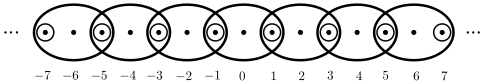
\includegraphics{Digital_line}}
\caption{The digital line topology.}
\label{F:Digital_line}
\end{center}
\end{figure}

In this exercise we explore the collection $\B = \{B(n)\}$. 

\ba
\item Show that the collection $\B = \{B(n)\}$ is a basis for a topology on $\Z$. (The resulting topology is called the \emph{digital line topology}\index{digital line topology} $\tau_{dl}$.\footnote{This digital line topology has applications in digital processing -- see \emph{Introduction to Topology: Pure and Applied} by Colin Adams and Robert Franzosa , Pearson Education, Inc., 2008,  Sections 1.4 and 11.3. The set $\Z$ with the digital line topology is called the \emph{digital line}.} (The digital line models a one-dimensional array of pixels, where the even integers are the pixels and the odd integers are boundaries between the pixels. Information about the \emph{digital plane} can be found in Section \ref{sec:Product_topology}.)


\item Determine which of the following sets are open in the digital line topology:
	\begin{enumerate}[i.]
	\item $\{0\}$
	\item $\{1\}$
	\item $\{0, 2\}$
	\item $\{1, 2, 3, 4, 5\}$
	\item $\Z^+$
	\item The set of odd integers.
	 \end{enumerate}
	 
\ea

\begin{comment}

\ExerciseSolution

\ba

\item Let $m \in \Z$ and suppose that $m$ is in $B_1 \cap B_2$ for some $B_1$ and $B_2$ in $\B$. Consider the case where $m$ is odd. Then $m \in B(m)$, $m \in B(m+1)$ and $m \in B(m-1)$. So $B_1$ and $B_2$ are one of $B(m)$, $B(m-1)$, and $B(m+1)$. In any case, $B(m)$ is then a subset of $B_1 \cap B_2$. 

Now consider the case where $m$ is even. Then $m \in B_(m)$ only. So $B_1 = B_2 = B(m)$, and $B(m) \subseteq B_1 \cap B_2$. We conclude that $\B$ is a basis for a topology on $\Z$. 

\item 	
	\begin{enumerate}[i.]
	\item The smallest open set that contains $0$ is $B(0) = \{-1,0,1\}$. So $\{0\}$ is not an open set. 
	\item Since $\{1\} = B(1)$, it follows that $\{1\}$ is an open set. 
	\item Any basis set that contains $0$ or $2$, also contains $1$. So $\{0, 2\}$ is not an open set. 
	\item Since $\{1, 2, 3, 4, 5\} = B(2) \cup B(4)$, it follows that the set $\{1, 2, 3, 4, 5\}$ is open.
	\item We can write $\Z^+$ as $\bigcup_{n \in \Z^+} B(n)$, so $\Z^+$ is an open set. 
	\item The set of odd integers can be written as $\bigcup_{n \text{ odd}} B(n)$, so the set of odd integers is an open set. 
	
	 \end{enumerate}

\ea

\end{comment}

\item \label{ex:TS_Zariski} Let $n$ be a positive integer and let $\mathcal{P}_n$ be the collection of all polynomials in $n$ real variables $x_1$, $x_2$, $\ldots$, $x_n$.  As a specific example, the polynomial 
\[f(x_1,x_2,x_3) = 2x_1x_3 + 5x_1x_2^2x_3^4 - x_2 + 10x_1^5x_3\]
is in $\mathcal{P}_3$. If $f(x_1, x_2, \ldots, x_n)$ is in $\mathcal{P}_n$, let $Z(f)$ be the set of zeros of the polynomial $f$. That is, 
\[Z(f) = \{(x_1, x_2, \ldots, x_n) \mid f(x_1,x_2, \ldots, x_n) = 0\}.\]
Note that $Z(f)$ is a subset of $\R^n$. For example, if $n=2$ and $f(x_1,x_2) = x_1^2 - x_2$ then $Z(f)$ is the set of ordered pairs in $\R^2$ satisfying $x_1^2-x_2 = 0$, or $x_2 = x_1^2$. This is the graph of the parabola $y=x^2$ in the plane. 

\ba

\item Describe $Z(f)$ in $\R^2$ if $f(x_1,x_2) = x_1^2 - 1$. 

\item If $E$ is a set of polynomials in $\mathcal{P}_n$, we let $Z(E) = \bigcap_{f \in E} Z(f)$ be the set of common zeros of all of the polynomials in $E$. Describe $Z(E)$ if $E = \{x_1+x_2+x_3, x_1-x_2-x_3, 3x_1+x_2+x_3\}$ in $\R^3$. 

%\item Let $E$ be a set of polynomials in $\mathcal{P}_n$. Prove or disprove $Z(E) = \bigcap_{f \in E} Z(f)$. 

\item Let $\mathcal{B}$ be the set of complements of the sets $Z(f)$ for $f \in \mathcal{P}_n$. Show that $\mathcal{B}$ is a basis for a topology on $\R^n$. The resulting topology is called the \emph{Zariski}\index{Zariski topology}\index{topology!Zariski} topology.

\item Is the set $S = \{(x_1,x_2) \in \R^2 \mid x_1 = 0 \text{ or } x_2 = 0\}$ an open set in $\R^2$ with the Zariski topology? Explain.  

\item Explain why the Zariski topology when $n=1$ is just the cofinite topology on $\R$. That is, show that every set that is open in the cofinite topology is open in the Zariski topology and that every set that is open in the Zaariski topology is open in the cofinite topology. 


\ea
 
\begin{comment}

\ExerciseSolution
 
\ba

 \item The zeros of the polynomial $f(x_1,x_2) = x_1^2 - 1$ occur when $x_1 = 1$ or $x_1 = -1$, while $x_2$ can take on any value. So $Z(x_1^2-1)$ is the union of the two lines $x=-1$ and $x=1$ in $\R^2$. 
 
 \item A little linear algebra shows that the reduced row echelon form of the matrix $\left[ \begin{array}{crr} 1&1&1 \\ 1&-1&-1 \\ 3&1&1 \end{array} \right]$ is $\left[ \begin{array}{ccc} 1&0&0 \\ 0&1&1 \\ 0&0&0 \end{array} \right]$. So $Z(E) = \{ (x_1,x_2,x_3) \mid x_2 = -x_3\}$ in $\R^3$. 

%\item Let $a \in Z(E)$ and let $f \in E$. Then $f(a) = 0$ and $a \in Z(f)$. It follows that $a \in \bigcap_{f \in E} Z(f)$. Now let $a \in \bigcap_{f \in E} Z(f)$. Then $f(a) = 0$ for every $f \in E$. Thus, $a \in Z(E)$. We conclude that $Z(E) = \bigcap_{f \in E} Z(f)$.

\item Let $a = (a_1,a_2,\ldots, a_n)$ be in $\R^n$. Let $f(x_1,x_2, \ldots, x_n) = 1$. Since $f(a) \neq 0$, $a \notin Z(f)$ and so $a \in \R^n \setminus Z(f)$. 

Now suppose that $B_1$ and $B_2$ are in $\mathcal{B}$ and $a \in B_1 \cap B_2$. Then $B_1 = \R^n \setminus Z(f_1)$ and $B_2 = \R^n \setminus Z(f_2)$ for some polynomials $f_1$ and $f_2$. Since $a \in B_1$, it follows that $f_1(a) \neq 0$. Similarly, since $a \in B_2$ we know that $f_2(a) \neq 0$. So $(f_1f_2)(a) = f_1(a)f_2(a) \neq 0$ and $a \notin Z(f_1f_2)$ and $a \in \R^n \setminus Z(f_1f_2)$. Thus, $\mathcal{B}$ is a basis for a topology on $\R^n$. 

\item The set $\{(0,x_2) \mid x_2 \in \R\}$ is $Z(x_1)$ while the set $\{(x_1,0) \mid x_1 \in \R\}$ is $Z(x_2)$. Now $B_1 = \R^2 \setminus Z(x_1)$ and $B_2 = \R^2 \setminus Z(x_2)$ are both open sets, and $S = B_1 \cap B_1$. As a finite intersection of open sets, we conclude that $S$ is an open set. 

\item Every polynomial in $\mathcal{P}_1$ has the form $ax+b$ where $a, b \in \R$. If $a \neq 0$, the only way $ax+b$ can have zeros is if $b = 0$. If $a \neq 0$ then the zeros of $ax+b$ are the same as the zeros of $x + \frac{b}{a}$. From this perspective we can just consider monic polynomials in $\mathcal{P}_1$. 

Let $O$ be an open set in $\R$ with the cofinite topology. Then $\R \setminus O$ is finite. Let $\R \setminus O = \{a_1, a_2, \ldots, a_k\}$. Let $f(x) = (x-a_1)(x-a_2) \cdots (x-a_k)$. Then $Z(f) = \R \setminus O$ and $\R \setminus Z(f) = O$. Thus, every set that is open in the cofinite topology is open in the Zariski topology.

To show that every open set in the Zariski topology is open in the cofinite topology, it suffices to show that this is true for the basis elements in the Zariski topology. Let $B = \R \setminus Z(f)$ be an open basis element in the Zariski topology, where $f$ is some polynomial in $\mathcal{P}_n$. Since $f$ can have only finitely many roots, the set $\R \setminus B = Z(f)$ is finite, and so $B$ is open in the cofinite topology. We conclude that the Zariski topology and cofinite topology are the same when $n =1$. Note that argument will not be valid when $n \geq 2$ because $Z(f)$ can be an infinite set.   

\ea

\end{comment}

\item For each of the following, answer true if the statement is always true. If the statement is only sometimes true or never true, answer false and provide a concrete example to illustrate that the statement is false. If a statement is true, explain why. 
	\ba
	\item The set $\{\emptyset, \{a,b\}, \{a,b,d,f\}, \{d,f\},X\}$ is a topology on the set $X = \{a,b,c,d,e,f\}$.

	\item  The set $\Z$ is an open subset of $\R$ using the finite complement topology $\tau_{FC}$ on $\R$.

	\item The set $\mathcal{B} = \{\{b\},\{c\}, \{a,b\}, \{b,c,d\}\}$ is a basis for the topology $\tau$ on the set $X = \{a,b,c,d\}$, where 
\[\tau = \{\emptyset, \{b\}, \{c\}, \{a,b\}, \{b,c\}, \{a,b,c\}, \{b,c,d\}, X\}.\]

	\item Let $X$ be a nonempty set. If $\tau$ is the discrete topology, then the topological set $(X,\tau)$ is metrizable.  

	\item The point $b$ is an interior point of the subset $A = \{a,b,d\}$ in the topological space $(X,\tau)$, where $X = \{a,b,c,d\}$ and 
\[\tau = \{\emptyset, \{a\}, \{a,b\}, \{c\}, \{d\}, \{c,d\}, \{a,c,d\}, \{a,c\}, \{a,d\}, \{a,b,c,\}, \{a,b,d\}, X\}.\]

	\item If $\tau_1$ and $\tau_2$ are topologies on a space $X$, then $\tau_1 \cup \tau_2$ is also a topology on $X$.  
	
	\item If $\tau_1$ and $\tau_2$ are topologies on a space $X$, then $\tau_1 \cap \tau_2$ is also a topology on $X$.
	
	\ea

\begin{comment}

\ExerciseSolution

\ba

	\item This statement is true. By definition, $\tau$ contains $\emptyset$ and $X$. The unions of the non-trivial sets in $\tau$ are 
	\[\{a,b\} \cup \{a,b,d,f\} = \{a,b,d,f\}, \{d,f\} \cup \{a,b,d,f\} = \{a,b,d,f\}, \text{ and } \{a,b\} \cup \{d,f\} = \{a,b,d,f\},\]
	and these unions are all in $\tau$. It is also the case that the intersections 
	\[\{a,b\} \cap \{a,b,d,f\} = \{a,b\}, \{d,f\} \cap \{a,b,d,f\} = \{d,f\}, \text{ and } \{a,b\} \cap \{d,f\} = \emptyset,\]
	of the non-trivial sets in $\tau$ are also in $\tau$. 
	
	\item  This statement is false since $\R \setminus \Z$ is not finite. 
	
	\item This statement is true. By inspection we can see that every element in $X$ is an element of some set in $\mathcal{B}$. Letting $B_1 = \{b\}$, $B_2 = \{c\}$, $B_3 = \{a,b\}$, and $B_4 = \{b,c,d\}$, we have that the intersections of the sets in $\mathcal{B}$ are 
	\begin{align*}
	B_1 \cap B_2 &= B_2 \cap B_3 = \emptyset, \\
	B_1 \cap B_i &= \{b\}, \text{ where } 3 \leq i \leq 4, \\
	B_2 \cap B_4 &= \{c\}, \text{ and } \\
	B_3 \cap B_4 &= \{b\}.
	\end{align*}
The only elements in $X$ that are in $B_i \cap B_j$ for some $i$ and $j$ are $b$ and $c$. But then either $B_1$ or $B_2$ is a subset of $B_i \cap B_j$. We conclude that $\mathcal{B}$ is a basis for $\tau$. 

	\item This statement is true since the topological space $(X,\tau)$ has the same open sets as the $(X, d)$, where $d$ is the discrete metric. 
	
	\item This statement is true since $\{a,b\}$ is an open set that contains $b$ and is also a subset of $A$. 

	\item This statement is false. Let $X = \{a,b,c\}$ with $\tau_1 = \{\emptyset, \{a\}, X\}$ and $\tau_2 =  \{\emptyset, \{b\}, X\}$. Then $\tau_1 \cup \tau_2 = \{\emptyset, \{a\}, \{b\}, X\}$. But $\{a\} \cup \{b\}$ is not in $\tau_1 \cup \tau_2$. 
		
	\item This statement is true. By definition, both $\emptyset$ and $X$ are in $\tau_1 \cap \tau_2$. Let $\{O_{\alpha}\}$ be a collection of sets in $\tau_1 \cap \tau_2$ for $\alpha$ in some indexing set $I$. Then each $O_{\alpha}$ is in $\tau_1$ and $\tau_2$, which means that $\bigcup_{\alpha \in I} O_{\alpha}$ is also in $\tau_1$ and $\tau_2$. Thus, $\bigcup_{\alpha \in I} O_{\alpha}$ is in $\tau_1 \cap \tau_2$. Similarly, if $I$ is finite, then $\bigcap_{\alpha \in I} O_{\alpha}$ is in $\tau_1$ and $\tau_2$, which means $\bigcap_{\alpha \in I} O_{\alpha}$ is in $\tau_1 \cap \tau_2$.
	
\ea

\end{comment}

\ee
  %12
\achapter{13}{Closed Sets in Topological Spaces}\label{sec:Closed_sets_topology}


\vspace*{-17 pt}
\framebox{
\parbox{\dimexpr\linewidth-3\fboxsep-3\fboxrule}
{\begin{fqs}
\item What does it mean for a set to be closed in a topological space?
\item What important properties do closed sets have in relation to unions and intersections?
\item What is a sequence in a topological space?
\item What does it mean for a sequence to converge in a topological space?
\item What is a limit of a sequence in a topological space?
\item What is a limit point of a subset of a topological space? How are closed sets related to limit points? 
\item What is a boundary point of a subset of a topological space and what is the boundary of a subset of a topological space? How are closed sets related to boundary points? 
\item What does it mean for a space to be Hausdorff? What important properties do Hausdorff spaces have?
\item What are the separation axioms $T_1$, $T_2$, $T_3$, and $T_4$. What is the underlying idea behind these properties?
\end{fqs}}}

\vspace*{13 pt}

\csection{Introduction}
We defined a closed set in a metric space to be the complement of an open set. Since a topology is defined in terms of open sets, we can make the same definition of closed set in a topological space. With the definition of closed set in hand, we can then ask if it is possible to define limit points, boundary, and closure in topological spaces and determine if there are corresponding properties for these ideas in topological spaces. 

\begin{definition} A subset $C$ of a topological space $X$ is \textbf{closed}\index{closed set in a topological space} if its complement $X \setminus C$ is open. 
\end{definition}

\begin{pa} ~
\be
\item List all of the closed sets in the indicated topological space.
	\ba
	\item $(X, \tau)$ with $X= \{a,b,c,d\}$ and $\tau = \{\emptyset, \{a\}, \{b\}, \{a,b\}, X \}$.

	\item $(X, \tau)$ with $X= \{a,b,c,d,e,f\}$ and $\tau = \{\emptyset,\{a\}, \{c,d\}, \{a,c,d\}, \{b,c,d,e,f\}, X\}$.

	\item $(X, \tau)$ with $X = \R$ and $\tau = \{\emptyset, \{0\}, \R\}$. 

	\item $(X, \tau)$ with $X = \{a,b,c\}$ and $\tau = \{\emptyset, \{a\}, \{b\},\{c\}, \{a,b\}, \{a,c\}, \{b,c\}, X \}$. (What is the name of this topology?)

	\item $(X, \tau)$ with $X=\Z^+$ and $\tau = \{\emptyset, X\}$ (this topology is called the \emph{indiscrete} or \emph{trivial} topology). 

	\ea


\item Using the examples from part (1), find (if possible), a set that is
	\ba
	\item both closed and open (if possible, find one that is not the entire set or the empty set)
	
	\item closed but not open
	
	\item open but not closed
	
	\item not open and not closed

	\ea

\item In $\R^n$ with the Euclidean metric, every single element set is closed. Does this property hold in the topological space $(X, \tau)$, where $X = \{a, b, c\}$ and $\tau = \{\emptyset, \{a\}, \{a, b\}, \{a, c\}, X\}$? Explain. 


\ee

\end{pa}

\begin{comment}

\ActivitySolution

\be
\item List all of the closed sets in the indicated topological space.
	\ba
	\item  The closed sets are the complements of the open sets, so the closed sets are 
\[X, \{b,c,d\}, \{a,c,d\}, \{c,d\}, \text{ and } \emptyset.\]

	\item  The closed sets are the complements of the open sets, so the closed sets are 
\[X, \{b,c,d,e,f\}, \{a,b,e,f\}, \{b,e,f\}, \{a\}, \text{ and } \emptyset.\]


	\item The closed sets are the complements of the open sets, so the closed sets are 
\[\R, \R-\{0\}, \text{ and } \emptyset.\]

	\item  Every subset is open, so this topology is the discrete topology. The closed sets are the complements of the open sets, so every subset is also closed. So the closed sets are 
\[X, \{b,c\}, \{a,c\}, \{a,b\}, \{c\}, \{b\},\{a\}, \text{ and } \emptyset.\]

	\item  The closed sets are the complements of the open sets, so the closed sets are 
\[X  \text{ and } \emptyset.\]

	\ea


\item 
	\ba
	\item  In the topological space $(X, \tau)$ with $X= \{a,b,c,d,e,f\}$ and $\tau = \{\emptyset,\{a\}, \{c,d\}, \{a,c,d\}, \{b,c,d,e,f\}, X\}$ the set $\{a\}$ is both open and closed. 
	
	\item  In the topological space $(X, \tau)$ with $X= \{a,b,c,d\}$ and $\tau = \{\emptyset, \{a\}, \{b\}, \{a,b\}, X \}$ the set $\{a,c,d\}$ is closed but not open. 
	
	\item  In the topological space $(X, \tau)$ with $X= \{a,b,c,d\}$ and $\tau = \{\emptyset, \{a\}, \{b\}, \{a,b\}, X \}$ the set $\{a,b\}$ is open but not closed. 
	
	\item  Consider the topological space $(X, \tau)$ with $X= \{a,b,c,d\}$ and $\tau = \{\emptyset, \{a\}, \{b\}, \{a,b\}, X \}$. The set $\{b,c\}$ is neither open nor closed. 
	
	\ea

\item Since $X \setminus \{a\} = \{b,c\}$ and $\{b,c\}$ is not open, the single element set $\{a\}$ is not closed. 

\ee

\end{comment}

\csection{Unions and Intersections of Closed Sets}

Now we have defined open and closed sets in topological spaces. In our preview activity we saw that a set can be both open and closed. As we did in metric spaces, we will call any set that is both open and closed a \emph{clopen}\index{clopen set in a topological space} (for closed-open) set.

By definition, any union and any finite intersection of open sets in a topological space is open, so the fact that closed sets are complements of open sets implies the following theorem. 

\begin{theorem} \label{thm:closed_TS} Let $X$ be a topological space.
\begin{enumerate}
\item Any intersection of closed sets in $X$ is a closed set in $X$.
\item Any finite union of closed sets in $X$ is a closed set in $X$. 
\end{enumerate}
\end{theorem}

\begin{proof} Let $X$ be a topological space. To prove part 1, assume that $C_{\alpha}$ is a collection of closed set in $X$ for $\alpha$ in some indexing set $I$. Then 
\[X \setminus \bigcap_{\alpha \in I} C_{\alpha} = \bigcup_{\alpha \in I} X \setminus C_{\alpha}.\]
The latter is an arbitrary union of open sets and so it an open set. By definition, then, $\bigcap_{\alpha \in I} C_{\alpha}$ is a closed set. 

For part 2, assume that $C_1$, $C_2$, $\ldots$, $C_n$ are closed sets in $X$ for some $n \in \Z^+$. To show that $C = \bigcap_{k=1}^n C_k$ is a closed set, we will show that $X \setminus C$ is an open set. Now 
\[X \setminus \bigcup_{\alpha \in I} C_{\alpha} = \bigcap_{\alpha \in I} X \setminus C_{\alpha}\]
is a finite intersection of open sets, and so is an open set. Therefore, $\bigcup_{\alpha \in I} C_{\alpha} $ is a closed set. 
\end{proof}

Theorem \ref{thm:closed_TS} tells us that any intersection of closed sets is closed, but only finite unions of closed sets are closed. How do we know that non-finite unions of closed sets aren't necessarily closed?

\begin{activity} Let $\Z$ be a topological space with the finite complement topology $\tau_{FC}$. That is, a non-empty set $O$ is open in $\Z$ if $\Z \setminus O$ is finite. 
	\ba
	\item What must be true about the cardinality of the closed sets in $(\Z, \tau_{FC})$? 
	
	\item Let $C_n = \{2, 3, \ldots, n\}$. Is the set $\bigcup_{n \geq 3} C_n$ a closed set in $(\Z, \tau_{FC})$? Explain. 

	\ea
	
\end{activity}
	
\begin{comment}

\ActivitySolution

\ba

\item If $C$ is closed, then $C$ is the complement of some open set $O$. That is, $C = \Z \setminus O$ is finite. 

\item Since $\bigcup_{n \geq 3} C_n = \{n \in \Z \mid n \geq 2\}$ is an infinite set, we can see that the union of all of the $C_n$ is not a closed set in $(\Z, \tau_{FC})$. We conclude that arbitrary unions of closed sets need not be closed. 

\ea

\end{comment}

\csection{Limit Points and Sequences in Topological Spaces}

Recall that we defined a limit point of a set $A$ in a metric space $X$ to be a point $x \in X$ such that every neighborhood of $x$ contains a point in $A$ different from $x$. Since we have defined neighborhoods in topological spaces, we can make the same definition. 

\begin{definition} Let $X$ be a topological space, and let $A$ be a subset of $X$. A \textbf{limit point}\index{limit point in a topological space} of $A$ is a point $x \in X$ such that every neighborhood of $x$ contains a point in $A$ different from $x$. 
\end{definition}

The set $A'$ of limit points of $A$ is called the \emph{derived set}\index{derived set} of $A$. 

\begin{activity} Find the limit point(s) of the following sets
\ba
\item $\{c,d\}$ in $(X, \tau)$ with $X= \{a,b,c,d\}$ and $\tau = \{\emptyset, \{a\}, \{b\}, \{a,b\}, X \}$

\item $\{a,b\}$ in the set $X= \{a,b,c,d,e,f\}$ with topology 
\[\tau= \{\emptyset,\{b\}, \{a,b,c\},\{d,e,f\},\{b,d,e,f\}, X\}.\] 

\item $\{a,b\} \subset X$ where $X = \{a,b,c\}$ in the discrete topology. 

\item $\{-1,0,1\} \subset \Z$ with $\tau$ the topology on $\Z$ with basis $\{B(n)\}$, where 
\[B(n) = \begin{cases} \{n\}	&\text{if $n$ is odd}, \\ \{n-1,n,n+1\}	&\text{if $n$ is even}. \end{cases}\]
(This topology is called the \emph{digital line topology} and has applications in digital processing. (This topology is called the \emph{digital line topology} and has applications in digital processing. That the collection $\{B(n)\}$ is a basis for a topology on $\Z$ is the topic of Exercise (\ref{ex:digital_line_topology}) on page \pageref{ex:digital_line_topology}.)
 
 \ea

\end{activity}

\begin{comment}

\ActivitySolution

\ba
\item  Neither $a$ nor $b$ is a limit point of $\{c,d\}$ since the open neighborhood $\{a,b\}$ contains no point in $\{c,d\}$ different than $a$ or $b$. The only open set that contains $c$ or $d$ is $X$, so that is the only neighborhood of $c$ or $d$. Since $X$ contains a point in $\{c,d\}$ that is different than $c$ (or $d$), both $c$ and $d$ are limit points of $\{c,d\}$. 

\item  None of the points $b$, $d$, $e$, or $f$ is a limit point of $\{a,b\}$ since the open neighborhood $\{b,d,e,f\}$ contains no point in $\{a,b\}$ different than $b$, $d$, $e$, or $f$. Any neighborhood of $a$ or $c$ must contain one of the open sets $\{a,b,c\}$ or $X$. So every neighborhood of $a$ or $c$ contains a point of $\{a,b\}$ different than $a$ or $c$. Therefore, the limit points of $\{a,b\}$ are $a$ and $c$ and $\{a,b\}' = \{a,c\}$. 

\item  For any $x \in \{a,b\}$, the open neighborhood $\{x\}$ of $x$ does not contain any points in $\{a,b\}$ different than $x$. So the set $\{a,b\}$ has no limit points. 

\item  Any neighborhood of $0$ must contain $B(0) = \{-1,0,1\}$, and so every neighborhood of $0$ contains a point in $\{-1,0,1\}$ different from $0$. Similarly, any neighborhood of $2$ must contain $B(2) = \{1,2,3\}$, and so every neighborhood of $2$ contains a point in $\{-1,0,1\}$ different from $2$. Also, any neighborhood of $-2$ must contain $B(-2) = \{-3,-2,-1\}$, and so every neighborhood of $-2$ contains a point in $\{-1,0,1\}$ different from $-2$. Thus, $\{-2,0,2\} \subseteq \{-1,0,1\}'$. If $n$ is odd, then the open neighborhood $B(n) = \{n\}$ contains no points of $\{-1,0,1\}$ different than $n$. So no odd integer is a limit point of $\{-1,0,1\}$. If $n$ is an even integer different than $-2$, $0$, and $2$, then the open neighborhood $B(n) = \{n-1,n,n+1\}$ contains no points in $\{-1,0,1\}$. Therefore, $\{-1,0,1\}' = \{-2,0,2\}$. 

\ea

\end{comment}

In metric spaces, a set is closed if and only if it contains all of its limit points. So the corresponding result in topological spaces should be no surprise. 

\begin{theorem} \label{thm:TS_closed_limitpoints} Let $C$ be a subset of a topological space $X$, and let $C'$ be the set of limit points of $C$. Then $C$ is closed if and only if $C' \subseteq C$.  
\end{theorem}

\begin{proof} Let $X$ be a topological space, and let $C$ be a subset of $X$. First we assume that $C$ is closed and show that $C$ contains all of its limit points. Let $x \in X$ be a limit point of $C$. We proceed by contradiction and assume that $x \notin C$. Then $x \in X \setminus C$, which is an open set. This means that there is a neighborhood (namely $X \setminus C$) of $x$ that contains no points in $C$, which contradicts the fact that $x$ is a limit point of $C$. We conclude that $x \in C$ and $C$ contains all of its limit points.

For the converse, assume that $C$ contains all of its limit points. To show that $C$ is closed, we prove that $X \setminus C$ is open. We again proceed by contradiction and assume that $X \setminus C$ is not open. Then there exists $x \in X \setminus C$ such that no neighborhood of $x$ is entirely contained in $X \setminus C$. This implies that every neighborhood of $x$ contains a point in $C$ and so $x$ is a limit point of $C$. It follows that $x \in C$, contradicting the fact that $x \in X \setminus C$. We conclude that $X \setminus C$ is open and $C$ is closed.
\end{proof}

In metric spaces we saw that limit point of a set is the limit of a sequence of points in the set. To explore this idea in topological spaces, we define sequences in the same way we did in metric spaces. 

\begin{definition} A \textbf{sequence}\index{sequence in a topological space} in a topological space $X$ is a function $f: \Z^+$ to $X$.
\end{definition}

We use the same notation and terminology related to sequences as we did in metric spaces: we will write $(x_n)$ to represent a sequence $f$, where $x_n = f(n)$ for each $ n \in \Z^+$. We can't define convergence in a topological space using a metric, but we can use open sets. Recall that a sequence $(x_n)$ in a metric space $(X,d)$ converges to a point $x$ in the space if, given $\epsilon > 0$ there exists a positive integer $N$ such that $d(x_n,x) < \epsilon$ for all $n \geq N$. In other words,  every open ball centered at $x$ contains all of the entries of the sequence past a certain point. We can replace open balls with open sets and make a similar definition of convergence in topological spaces. 

\begin{definition} A sequence $(x_n)$ in a topological space $X$ \textbf{converges}\index{convergent sequence in a topological space} to the point $x \in X$ if, for each open set $O$ that contains $x$ there exists a positive integer $N$ such that $x_n \in O$ for all $n \geq N$. 
\end{definition}

If a sequence $(x_n)$ converges to a point $x$, we call $x$ a \emph{limit}\index{limit of a sequence in a topological space} of the sequence $(x_n)$. 

\begin{activity} \label{act:TS_limits} In metric spaces, limits of sequences are unique. We may wonder if the same result is true in topological spaces. Consider the topological space $(X,\tau)$, where $X = \{a, b, c\}$ and $\tau = \{\emptyset, \{c\}, \{a, c\}, \{b, c\}, X\}$. Find all limits of all constant sequences in $X$.

\end{activity}

\begin{comment}

\ActivitySolution We start by finding all neighborhoods. 
\begin{itemize}
\item The neighborhoods of $a$ are $\{a,c\}$ and $X$.
\item The neighborhoods of $b$ are $\{b,c\}$ and $X$.
\item The neighborhoods of $c$ are $\{c\}$, $\{a,c\}$, $\{b,c\}$, and $X$.
\end{itemize}

Consider the sequence $(a)$. The neighborhood $\{b,c\}$ of $b$ does not contain $a$, so $b$ is not a limit of the sequence $(a)$. The neighborhood $\{c\}$ of $c$ does not contain $a$, so $c$ is not a limit of the sequence $(a)$. Therefore, the only limit of the sequence $(a)$ is $a$.

Now consider the sequence $(b)$. The neighborhood $\{a,c\}$ of $a$ does not contain $b$, so $a$ is not a limit of the sequence $(a)$. The neighborhood $\{c\}$ of $c$ does not contain $b$, so $c$ is not a limit of the sequence $(b)$. Therefore, the only limit of the sequence $(b)$ is $b$.

Finally, consider the sequence $(c)$.  Each neighborhood of $a$ and $b$ contains the entire sequence $(c)$, so $a$ and $b$ are both limits of $(c)$. It follows that every point in $X$ is a limit of the sequence $(a)$.

\end{comment}


The result of Activity \ref{act:TS_limits} is that sequences do not behave in topological spaces as we would expect them to. Consequently, sequences do not play the same important role in topological spaces as they do in metric spaces. However, the concept of limit point is important, as are the notions of boundary and closure in topological spaces. 

\csection{Closure in Topological Spaces}

Once we have a definition of limit point, we can define the closure of a set just as we did in metric spaces. 

\begin{definition} The \textbf{closure}\index{closure in topological spaces} of a subset $A$ of a topological space $X$ is the set 
\[\overline{A} = A \cup A'.\]
\end{definition}

In other words, the closure of a set is the collection of the elements of the set and the limit points of the set. The following theorem is the analog of the theorem in metric spaces about closures. 

\begin{theorem} \label{thm:TS_closure_closed} Let $X$ be a topological space and $A$ a subset of $X$. The closure of a $A$ is a closed set. Moreover, the closure of $A$ is the smallest closed subset of $X$ that contains $A$. 
\end{theorem}

\begin{proof} Let $X$ be a topological space and $A$ a subset of $X$. To prove that $\overline{A}$ is a closed set, we will prove that $\overline{A}$ contains its limit points. Let $x \in \overline{A}'$. To show that $x \in \overline{A}$, we proceed by contradiction and assume that $x \notin \overline{A}$. This implies that $x \notin A$ and $x \notin A'$. Since $x \notin A'$, there exists a neighborhood $N$ of $x$ that contains no points of $A$ other than $x$. But $A \subseteq \overline{A}$ and $x \notin \overline{A}$, so it follows that $N \cap A = \emptyset$. This implies that there is an open set $O \subseteq N$ centered at $x$ so that $O \cap A = \emptyset$. The fact that $x \in \overline{A}'$ means that $O \cap \overline{A}$ contains a point $y$ in $\overline{A}$ different from $x$. Since $O \cap A = \emptyset$, we must have $y \in A'$. But the fact that $O$ is a neighborhood of $y$ means that $O$ must contain a point of $A$ different than $y$, which contradicts the fact that $O \cap A = \emptyset$. We conclude that $x \in \overline{A}$ and $\overline{A}' \subseteq \overline{A}$. This shows that $\overline{A}$ is a closed set. 

The proof that $\overline{A}$ is the smallest closed subset of $X$ that contains $A$ is left for the next activity.
\end{proof}

\begin{activity} Let $(X,d)$ be a topological space, and let $A$ be a subset of $X$. 
\ba
\item What will we have to show to prove that $\overline{A}$ is the smallest closed subset of $X$ that contains $A$?

\item Suppose that $C$ is a closed subset of $X$ that contains $A$. To show that $\overline{A} \subseteq C$, why is it enough to demonstrate that $A' \subseteq C$? 

\item If $x \in A'$, what can we say about $x$? 

\item Complete the proof that $\overline{A} \subseteq C$.

\ea

\end{activity}

\begin{comment}

\ActivitySolution

\ba
\item We need to prove that any closed subset of $X$ that contains $A$ also contains $\overline{A}$.

\item Since $\overline{A} = A \cup A'$, if $C$ already contains $A$, then to show that $\overline{A} \subseteq C$, we only need to show that $A' \subseteq C$. 

\item If $x \in A'$, then $x$ is a limit point of $A$. That means that every neighborhood of $x$ in $X$ contains a point in $A$ different from $x$.

\item Let $x \in A'$, and let $N$ be a neighborhood of $x$. Then $N$ contains a point of $A$ different than $x$. Since $A \subseteq C$, it follows that $N$ contains a point of $C$ different than $x$. So $x$ is a limit point of $C$. The fact that $C$ is closed means that $C$ contains its limit points, so $x \in C$. Therefore, $A' \subseteq C$ and $\overline{A} \subseteq C$. 

\ea

\end{comment}

One consequence of Theorem \ref{thm:TS_closure_closed} is the following.

\begin{corollary} A subset $C$ of a topological space $X$ is closed if and only if $C = \overline{C}$. 
\end{corollary}

\csection{The Boundary of a Set}

In addition to limit points, we also defined boundary points in metric spaces. Recall that a boundary point of a set $A$ in a metric space $X$ could be considered to be any point in $\overline{A} \cap \overline{X \setminus A}$. We make the same definition in a topological space. 

\begin{definition} Let $(X, \tau)$ be a topological space, and let $A$ be a subset of $X$. A \textbf{boundary point}\index{boundary point in a topological space} of $A$ is a point $x \in X$ such that every neighborhood of $x$ contains a point in $A$ and a point in $X \setminus A$. The \textbf{boundary}\index{boundary in a topological space} of $A$ is the set 
\[\Bdry(A) = \{x \in X \mid x \text{ is a boundary point of } A\}.\]
\end{definition}

As with metric spaces, the boundary points of a set $A$ are those points that are ``between" $A$ and its complement. 

\begin{activity} \label{act:TS_bl_examples} Find the boundaries of the following sets
\ba
\item $\{c,d\}$ in $(X, \tau)$ with $X= \{a,b,c,d\}$ and $\tau = \{\emptyset, \{a\}, \{b\}, \{a,b\}, X \}$.

\item $\{a,b\}$ in the set $X= \{a,b,c,d,e,f\}$ with topology 
\[\tau= \{\emptyset,\{b\}, \{a,b,c\},\{d,e,f\},\{b,d,e,f\}, X\}.\] 

\item $\{a,b\} \subset X$ where $X = \{a,b,c\}$ in the discrete topology.

\item $\Z$ in $\R$ with the finite complement topology $\tau_{FC}$. 

\ea

\end{activity}

\begin{comment}

\ActivitySolution

\ba
\item  Neither $a$ nor $b$ is a boundary point of $\{c,d\}$ since the open neighborhood $\{a,b\}$ contains no point in $\{c,d\}$. The only open set that contains $c$ or $d$ is $X$, so that is the only neighborhood of $c$ or $d$. Since $X$ contains a point in $\{c,d\}$ that is different than $c$ (or $d$), and a point not in $\{c,d\}$, both $c$ and $d$ are boundary points of $\{c,d\}$. Therefore, $\Bdry(\{c,d\}) = \{c,d\}$. 

\item  None of the points $d$, $e$, or $f$ is a boundary point of $\{a,b\}$ since the open neighborhood $\{d,e,f\}$ contains no point in $\{a,b\}$. The open neighborhood $\{b\}$ of $b$ contains no points that are not in $\{a,b\}$, so $b$ is not a boundary point of $\{a,b\}$. Any neighborhood of $a$ or $c$ must contain one of the open sets $\{a,b,c\}$ or $X$. So every neighborhood of $a$ or $c$ contains a point of $\{a,b\}$ and a point not in $\{a,b\}$. So $a$ and $c$ are boundary points of $\{a,b\}$. Therefore, $\Bdry(\{a,b\}) = \{a,c\}$.  

\item Since $\{a\}$, $\{b\}$, and $\{c\}$ are open sets, and none of these sets contain points in both $A$ and $X \setminus A$, the boundary of $A$ is empty. 

\item Let $x \in \R$ and let $O$ be an open set containing $x$. Since $\R \setminus O$ is finite, there must be infinitely many points in both $\Z$ and $\R$ that are not in $\R \setminus O$. So $O$ contains infinitely many integers and real numbers. It follows that every point in $\Z$ is a boundary point and $\Bdry(\Z) = \R$. 

\ea

\end{comment}

Just as with metric spaces, we can characterize the closed sets as the sets that contain their boundary.

\begin{theorem} \label{thm:TS_Closed_boundary} A subset $C$ of a topological space $X$ is closed if and only if $C$ contains its boundary. 
\end{theorem}

The proof of Theorem \ref{thm:TS_Closed_boundary} is left to Exercise (\ref{ex:TS_Closed_boundary}).

\csection{Separation Axioms}

As we have seen, sequences in topological spaces do not generally behave as we would expect them to. As a result, we look for conditions on topological spaces under which sequences do exhibit some regular behavior. In our preview activity we saw that in it is possible in a topological space that single point sets do not have to be closed. In Activity \ref{act:TS_limits}, we also saw that limits of sequences in topological spaces are not necessarily unique. This type of behavior limits the results that one can prove about such spaces. As a result, we define classes of topological spaces whose behaviors are closer to what our intuition suggests. 

\begin{activity} \label{act:Hausdorff} ~
\ba
\item Consider a metric space $(X,d)$, and let $x$ and $y$ be distinct points in $X$. 
	\begin{enumerate}[i.]
	\item Explain why $x$ and $y$ cannot both be limits of the same sequence if we can find disjoint open balls $B(x,r)$ centered at $x$ and $B(y,s)$ centered at $y$ such that $B_x \cap B_y = \emptyset$.
	
	\item Now show that we can find disjoint open balls $B(x,r)$ centered at $x$ and $B(y,s)$ centered at $y$ such that $B(x,s) \cap B(y,r) = \emptyset$.
	
	\end{enumerate}

\item Return to our example from Activity \ref{act:TS_limits} with $X = \{a, b, c\}$ and topology 
\[\tau~=~\{\emptyset, \{c\}, \{a, c\}, \{b, c\}, X\}.\] 
We saw that every point in $X$ is a limit of the constant sequence $(c)$. If $x \neq c$ in $X$, Explain why there are no disjoint open sets $O_x$ containing $x$ and $O_c$ containing $c$. 	

\ea

\end{activity}

\begin{comment}

\ActivitySolution

\ba
\item Consider a metric space $(x,d)$, and let $x$ and $y$ be distinct points in $X$. 
	\begin{enumerate}[i.]
	\item Suppose a sequence $(x_n)$ has $x$ as a limit. Then there exists a positive integer $N$ such that $n \geq n$ implies $x_n \in B(x,r)$. But then $x_n \notin B(y,s)$ and so $y$ cannot be a limit of the sequence $(x_n)$. 
	
	\item Let $r = \frac{d(x,y)}{2}$. To show that $B(x,r) \cap B(y,r) = \emptyset$, suppose $z \in (B(x,r) \cap B(y,r)$. Then $z \in B(x,r)$. The triangle inequality $d(x,y) \leq d(x,z) + d(z,y)$ shows that 
	\[d(z,y) \geq d(x,y) - d(x,z) > d(x,y) - r = 2r -r = r.\]
	But this contradicts $z \in B(y,r)$. We conclude that $B(x,r) \cap B(y,r) = \emptyset$.
	
	\end{enumerate}

\item The only open sets that contain $a$ are $\{a,c\}$ and $X$ and the only open sets that contain $b$ are $\{b,c\}$ and $X$. These open sets all contain $c$, so there are no disjoint open sets $O_x$ and $O_c$ containing $x$ and $c$. 	

\ea

\end{comment}

It is the fact as described in Activity \ref{act:Hausdorff} that we can separate disjoint points by disjoint open sets that separates metric spaces from other spaces where limits are not unique. If we restrict ourselves to spaces where we can separate points like this, then we might expect to have unique limits. Such spaces are called \emph{Hausdorff} spaces. 

\begin{definition} A topological space $X$ is a \textbf{Hausdorff}\index{Hausdoff space} space if for each pair $x$, $y$ of distinct points in $X$, there exists open sets $O_x$ of $x$ and $O_y$ of $y$ such that $O_x \cap O_y = \emptyset$. 
\end{definition}

Activity \ref{act:Hausdorff} shows that every metric space is a Hausdorff space. Once we start imposing conditions on topological spaces, we restrict the number of spaces we consider.

\begin{activity} ~
\ba
\item Let $X$ be any set and $\tau$ the discrete topology. Is $(X, \tau)$ Hausdorff? Justify your answer.

\item Let $(X, \tau)$ be a Hausdorff topological space with $X = \{x, x_1, x_2, \ldots, x_n\}$ a finite set. Let $x \in X$. Is $\{x\}$ an open set? Explain. What does this say about the topology $\tau$? (Hint: Is $x$ a limit point of $\{x_1, x_2, \ldots, x_n\}$?)

\ea

\end{activity}

\begin{comment}

\ActivitySolution

\ba
\item Let $x$ and $y$ be distinct elements in $X$. Since every subset of $X$ is open, the disjoint open set $\{x\}$ and $\{y\}$ separate $x$ and $y$. So $(X, \tau)$ is Hausdorff.

\item Suppose $X = \{x, x_1, x_2, \ldots, x_n\}$. Let $A = \{x_1, x_2, \ldots, x_n\}$. We will show that $A$ is closed by demonstrating that $A$ contains all of its limit points. To do this we only need to show that $x$ is not a limit point of $A$. Since $X$ is Hausdorff, for each $i$ there exists an open sets $Ox_i$ and $O_i$ such that $Ox_i \cap O_i = \emptyset$. Let $O = \cap Ox_i$. Then $O$ is neighborhood of $x$ and $O \cap O_i = \emptyset$ for every $i$. Thus, $O$ does not contain any points in $A$. Since $A$ is closed, it follows that $\{x\} = X \setminus A$ is open. Since every single element set is open, the topology $\tau$ is the discrete topology. 

\ea

\end{comment}

\begin{example} \label{exp:K_topology} There are examples of Hausdorff spaces that are not the standard metric spaces. For example, Let  $K = \left\{\frac{1}{k} \mid k \text{ is a positive integer} \right\}$. We use $K$ to make a topology on $\R$ with basis all open intervals of the form $(a,b)$ and all sets of the form $(a,b) \setminus K$, where $a < b$ are real numbers. This topology adds the extra intervals of the form $(a,b) \setminus K$ to the standard open intervals to make a new topology. This topology is known as the $K$-topology on $\R$. Just as in $(\R, d_E)$, if $x$ and $y$ are distinct real numbers we can separate $x$ and $y$ with open intervals. 


\end{example}

The reason we defined Hausdorff spaces is because they have familiar properties, as the next theorems illustrate. 

\begin{theorem} Each single point subset of a Hausdorff topological space is closed.
\end{theorem}

\begin{proof} Let $X$ be a Hausdorff topological space, and let $A = \{a\}$ for some $a \in X$. To show that $A$ is closed, we prove that $X \setminus A$ is open. Let $x \in X \setminus A$. Then $x \neq a$. So there exist open sets $O_x$ containing $x$ and $O_a$ containing $a$ such that $O_x \cap O_a = \emptyset$. So $a \notin O_x$ and $O_x \subseteq X \setminus A$. Thus, every point of $X \setminus A$ is an interior point and $X \setminus A$ is an open set. This verifies that $A$ is a closed set.
\end{proof}


\begin{theorem} A sequence of points in a Hausdorff topological space can have at most one limit in the space.
\end{theorem}

\begin{proof} Let $X$ be a Hausdorff topological space, and let $(x_n)$ be a sequence in $X$. Suppose $(x_n)$ converges to $a \in X$ and to $b \in X$. Suppose $a \neq b$. Then there exist open sets $O_a$ of $a$ and $O_b$ of $b$ such that $O_a \cap O_b = \emptyset$. But the fact that $(x_n)$ converges to $a$ implies that there is a positive integer $N$ such that $x_n \in O_a$ for all $n \geq N$. But then $x_n \notin O_b$ for any $n \geq N$. This contradicts the fact that $(x_n)$ converges to $b$. We conclude that $a=b$ and that the sequence $(x_n)$ can have at most one limit in $X$. 
\end{proof}

Hausdorff spaces are important because we can separate distinct points with disjoint open sets. It is also of interest to consider what other types of objects we can separate with disjoint open sets. For example, the indiscrete topology is quite bad in the sense that its open sets can't distinguish between distinct points. That is, if $x$ and $y$ are distinct points in a space with the indiscrete topology, then every open set that contains $x$ also contains $y$. By contrast, in a Hausdorff space we can separate distinct points with disjoint open sets. This is an example of what is called a ``separation" property. Other types of separation properties describe different types of topological spaces. These separation properties determine what kind of objects we can separate with disjoint open sets -- e.g., points, points and closed sets, closed sets and closed sets. The following are the most widely used separation properties. These properties rule out kinds of unwelcome properties that a topological space might have. For example, recall that limits of sequences are unique in Hausdorff spaces. (We traditionally call these separation properties ``axioms" because we generally assume that our topological spaces have these properties. However, these are not axioms in the usual sense of the word, but rather properties.)

\begin{definition} Let $X$ be a topological space. 
\begin{enumerate}

\item The space $X$ is a \textbf{\emph{T}$_1$-space}\index{$T_1$-space} or \textbf{Frechet space}\index{Frechet space} if for every $x\neq y$ in $X$, there exist an open set $U$ containing $y$ such that $x \notin U$.  

\item The space $X$ is a \textbf{\emph{T}$_2$-space}\index{$T_2$-space} or a \textbf{Hausdorff space} if for every $x\neq y$ in $X$, there exist disjoint open sets $U$ and $V$ such that $x\in U$ and $y\in V$.

\item The space $X$ is \textbf{regular}\index{regular topological space} if for each closed set $C$ of $X$ and each point $x \in X \setminus C$, there exists disjoint open sets $U$ and $V$ in $X$ such that $C \subseteq U$ and $x \in V$. The space $X$ is a \textbf{\emph{T}$_3$-space}\index{$T_3$-space} or a \textbf{regular Hausdorff space} if $X$ is a regular $T_1$ space. 

\item The space $X$ is a \textbf{normal}\index{normal topological space} space if for each pair $C$ and $D$ of disjoint closed subsets of $X$ there exist disjoint open sets $U$ and $V$ such that $C \subseteq U$ and $D \subseteq V$.  The space $X$ is a \textbf{\emph{T}$_4$-space}\index{$T_4$-space} or a \textbf{normal Hausdorff space} if $X$ is a normal $T_1$ space. 

\end{enumerate}
\end{definition}
The use of the variable $T$ comes from the German ``Trennungsaxiome" for separation axioms. Note again that these are not technically axioms, but rather properties. An interesting question is why we insist that $T_3$ and $T_4$-spaces also be $T_1$. We want these axioms to provide more separation at the index increases. Consider a space $X$ with the indiscrete topology. In this space, nothing is separated. However, this space is vacuously regular and normal. To avoid this seeming incongruity, we insist on working only with $T_1$ spaces. Note that a space with the indiscrete topology is not $T_1$. 

It is the case that every $T_4$-space is $T_3$, every $T_3$-space is $T_2$, and every $T_2$-space is $T_1$. Verification of these statements are left to Exercise (\ref{ex:T_1_2_3}). These properties are also all different. That is, there are $T_1$-spaces that are not $T_2$ and $T_2$-spaces that are not $T_3$. These problems are given in Exercise (\ref{ex:not_T_1_2_3}). The fact that there are $T_3$-spaces that are not $T_4$ is a bit difficult. An example is the \emph{Niemytzki plane}. The Niemytzki plane is the upper half plane $X = \{(x,y) \in \R^2 \mid y \geq 0\}$. Let $L$ be the boundary of $X$. That is, $L = \{(x,y) \in \R^2 \mid y = 0\}$.  A basis for the topology on $X$ consists of the standard open disks centered at points with $y > 0$ along with the open disks in $X \setminus L$ that are tangent to $L$ together with their points of tangency. We won't verify that the Niemytzki plane is $T_3$ but not $T_4$. The interested reader can find an accessible proof in the article ``Another Proof that the Niemytzki Plane is not Normal" by David H. Vetterlein in the \emph{Pi Mu Epsilon Journal}, Vol. 10, No. 2 (SPRING 1995), pp. 119-121. 
 
 

\csection{Summary}
Important ideas that we discussed in this section include the following.
\begin{itemize}
\item A subset $C$ of a topological space $X$ is closed if $X \setminus C$ is open.
\item Any intersection of closed sets is closed, while unions of finitely many closed sets are closed. 
\item A sequence in a topological space $X$ is a function $f: \Z^+$ to $X$.
\item A sequence $(x_n)$ in a topological space $X$ converges to a point $x$ in $X$ if for each open set $O$ containing $x$, there exists a positive integer $N$ such that $x_n \in O$ for all $n \geq N$. 
\item If a sequence $(x_n)$ in a topological space $X$ converges to a point $x$, then $x$ is a limit of the sequence $(x_n)$. 
\item A limit point of a subset $A$ of a topological space $X$ is a point $x \in X$ such that every neighborhood of $x$ contains a point in $A$ different from $x$. A subset $C$ of a topological space $X$ is closed if and only if $C$ contains all of its limit points.   
\item A boundary point of a subset $A$ of a topological space $X$ is a point $x \in X$ such that every neighborhood of $x$ contains a point in $A$ and a point in $X \setminus A$. The boundary of $A$ is the set 
\[\Bdry(A) = \{x \in X \mid x \text{ is a boundary point of } A\}.\]
A subset $C$ of $X$ is closed if and only if $C$ contains its boundary. 
\item A topological space $X$ is Hausdorff if we can separate distinct points with open sets in the space. That is, if for each pair $x$, $y$ of distinct points in $X$, there exists open sets $O_x$ of $x$ and $O_y$ of $y$ such that $O_x \cap O_y = \emptyset$. 
Hausdorff spaces are important because sequences have unique limits in Hausdorff spaces and single point sets are closed. 
\item Separation axioms tell us what kinds of objects can be separated by open sets. 
	\begin{itemize}
	\item In a $T_1$-space, we can separate two distinct points with one open set. That is, given distinct points $x$ and $y$ in a $T_1$ topological space $X$, there is an open set $U$ that separates $y$ from $x$ in the sense that $y \in U$ but $x \notin U$. 
	\item In a $T_2$-space $X$ we can separate points more distinctly. That is, if $x$ and $y$ are different points in $X$, there exist disjoint open sets $U$ and $V$ such that $x \in U$ and $y \in V$. 
	\item In a $T_3$-space $X$ we can separate a point from a closed set that does not contain that point. That is, if $C$ is a closed subset of $X$ and $x$ is a point not in $C$, there exists disjoint open sets $U$ and $V$ in $X$ such that $C \subseteq U$ and $x \in V$. 
	\item In a $T_4$-space $X$ we can separate disjoint closed sets. That is, if $C$ and $D$ are disjoint closed subsets of $X$, there exist disjoint open sets $U$ and $V$ such that $C \subseteq U$ and $D \subseteq V$.  
	\end{itemize}
	
\end{itemize}

\csection{Exercises}

\be

\item Determine exactly which finite topological spaces are Hausdorff. Prove your result.

\begin{comment}

\ExerciseSolution We will show that a finite topological space $(X,\tau)$ is Hausdorff if and only if $\tau$ is the discrete topology. Let $(X, \tau)$ be a finite topological space. Suppose that $X$ is Hausdorff. To prove that $\tau$ is the discrete metric, we show that every singleton set is open. Let $x \in X$. Since $X$ is Hausdorff, for every $y \in X$ there are open sets $O_x$ and $O_y$ such that $x \in O_x$, $y \in O_y$, and $O_x \cap O_y = \emptyset$.  Let $O = \bigcup_{\substack{y \ in X \\ y \neq x}} O_y$. Since there are only finite many points $y$, the set $O$ is a finite union of open sets and so $O$ is an open set. For each $y \in X \setminus \{x\}$, we know that $y  \in O_y$. Also, no $O_y$ contains $x$. So $O = X \setminus \{x\}$. Thus, $\{x\} = X \setminus O$ and so $\{x\}$ is an open set. It follows that $\tau$ is the discrete metric.

Now suppose that $\tau$ is the discrete metric. To show that $X$ is Hausdorff, let $x$, $y$ be distinct points in $X$. Then $\{x\}$ and $\{y\}$ are open and separate $x$ and $y$, so $X$ is Hausdorff. 

\end{comment}

\item Let $(X, \tau)$ be a topological space and let $A$ be a subset of $X$. Prove that $\overline{A} = A \cup \Bdry(A)$. 

\begin{comment}

\ExerciseSolution Let $A$ be a subset of a topological space $X$. To prove that $\overline{A} = A \cup \Bdry(A)$ we demonstrate the containment in both directions. Let $x \in \overline{A}$. Then $x \in A$ or $x \in A'$. We consider the cases.
\begin{itemize}
\item Suppose that $x \in A$. Then $x \in A \cup \Bdry{A}$ and we are done.
\item Suppose $x \notin A$ and $x \in A'$. We show that $x \in \Bdry(A)$. Let $N$ be a neighborhood of $x$. Since $x \in A'$, we know that $N$ contains a point in $A$ different than $x$. But $x \notin A$, so $N$ contains a point in $A$ and a point not in $A$. Thus, $x \in \Bdry(A) \subseteq A \cup \Bdry(A)$. 
\end{itemize}
In either case we have $x \in A \cup \Bdry(A)$ and so $\overline{A} \subseteq A \cup \Bdry(A)$. 

For the reverse containment, let $x \in A \cup \Bdry(A)$. Then $x \in A$ or $x \in \Bdry(A)$. We consider the cases.
\begin{itemize}
\item Suppose that $x \in A$. Then $x \in A \cup A'$ and we are done.
\item Suppose $x \notin A$ and $x \in \Bdry(A)$. We show that $x \in A'$. Let $N$ be a neighborhood of $x$. Since $x \in \Bdry(A)$, we know that $N$ contains a point in $A$ and a point in $X \setminus A$. But $x \notin A$, so $N$ contains a point in $A$ different from $x$. Thus, $x \in A' \subseteq \overline{A}$. 
\end{itemize}
In either case we have $x \in \overline{A}$ and so $A \cup \Bdry(A) \subseteq \overline{A}$. Combining the containments gives us $A \cup \Bdry(A) =\overline{A}$.

\end{comment}

\item Let $A$ a subset of a topological space. Prove that $\Bdry(A) = \emptyset$ if and only if $A$ is open and closed.

\begin{comment}

\ExerciseSolution Let $A$ a subset of of a topological space $X$. First we show that $\Bdry(A) = \emptyset$ implies that $A$ is open and closed. Assume $\Bdry(A) = \overline{A} \cap \overline{X \setminus A} = \emptyset.$ To prove that $A$ is closed, we will demonstrate that $A = \overline{A}.$ Since we know that $A \subset \overline{A}$ for any set $A$, we only need show that $\overline{A} \subset A.$ We proceed by contradiction. Assume $\overline{A} \not\subset A,$ that is there exists a point $x \in \overline{A} \setminus A.$ Thus, $x$ is in both $\overline{A}$ and $X \setminus A$. We know that $X \setminus A \subset \overline{X \setminus A},$ so $x \in \overline{X \setminus A}.$ Therefore, $x \in \overline{A} \cap \overline{X \setminus A} = \Bdry(A).$ This is a contradiction to our assumption that $\Bdry(A) = \emptyset.$ Therefore we must have that $\overline{A} \subset A$ and $A$ is closed. 

To show $A$ is open, we will demonstrate that $X \setminus A$ is closed. Let $B = X \setminus A$. Note that 
\[\Bdry(B) = \overline{B} \cap \overline{X \setminus B)} = \overline{X \setminus A} \cap \overline{A} = \Bdry(A) = \emptyset.\]
The proof in the previous paragraph shows that $B = X \setminus A$ is closed. Therefore, $A$ is open. 

For the converse, assume that $A$ is both open and closed. Then $A$ and $X \setminus A$ are closed. So $\overline{A} = A$ and $\overline{X \setminus A} = X \setminus A$. So 
\[\Bdry(A) = \overline{A} \cap \overline{X \setminus A} = A \cap (X \setminus A) = \emptyset.\]

\end{comment}


\item Let $X$ be a nonempty set with at least two elements and let $p$ be a fixed element in $X$. Let $\tau_p$ be the particular point topology and $\tau_{\overline{p}}$ the excluded point topology on $X$. That is
\begin{itemize}
\item $\tau_{p}$ is the collection of subsets of $X$ consisting of $\emptyset$, $X$, and all of the subsets of $X$ that contain $p$.  
\item $\tau_{\overline{p}}$ is the collection of subsets of $X$ consisting of $\emptyset$, $X$, and all of the subsets of $X$ that do not contain $p$. 
\end{itemize}
That the particular point and excluded point topologies are topologies is the subject of Exercises (\ref{ex:particular_point_topology}) and (\ref{ex:excluded_point_topology}) on page \pageref{ex:particular_point_topology}. 

Let $A = (0,1]$ be a subset of $\R$. Find, with proof, $\overline{A}$, $\Int(A)$, and $\Bdry(A)$ when
	\ba
	\item $\R$ has the topology $\tau_{p}$ with $p = 0$
	
	\item $\R$ has the topology $\tau_{\overline{p}}$ with $p = 0$.
	
	\ea
	
\begin{comment}

\ExerciseSolution

	\ba
	\item 
	\begin{itemize}
	\item Since $\R \setminus A = (-\infty,0] \cup (1,\infty)$ contains $0$, we see that $\R \setminus A$ is open. This makes $A$ a closed set, so $\overline{A} = A$. 
	\item We know that $\Int(A)$ is the largest open set contained in $A$. But no nonempty subset of $A$ is open, since $0 \notin A$. Thus, $\Int(A) = \emptyset$. 
	\item Recall that $\Bdry(A) = \overline{A} \cap \overline{\R \setminus A}$. To determine $\overline{\R \setminus A}$, we note that $\overline{\R \setminus A}$ is the smallest closed set that contains $\R \setminus A$. Any set $B$ that contains $\R \setminus A$ also contains $0$, so $\R \setminus B$ does not contain $0$ and is therefore not open. Thus, the only closed set that contains $\R \setminus A$ is $\R$, and so $\overline{\R \setminus A} = \R$. This makes $\Bdry(A) = \overline{A} \cap \overline{\R \setminus A} = \overline{A} = A$. 
	\end{itemize}
	
\item 
	\begin{itemize}
	\item To find $\overline{A}$, we use the fact that $\overline{A}$ is the smallest closed set that contains $A$. Let $B$ be a closed set that contains $A$. Since $B$ is closed, we know that $\R \setminus B$ is open and that $0$ is not in $\R \setminus B$. Thus, $0 \in B$. The smallest set that contains both $A$ and $0$ is $[0,1]$, so $\overline{A} = [0,1]$. 
	\item Since $A$ does not contain $0$, it is the case that $A$ is open and so $\Int(A) = A$. 
	\item The fact that $A$ is open means that $\R \setminus A$ is closed and so $\overline{\R \setminus A} = \R \setminus A$. Then 
	\[\Bdry(A) = \overline{A} \cap \overline{\R \setminus A} = [0,1] \cap \left((-\infty,0] \cup (1,\infty)\right) = \{0\}.\]
	\end{itemize}
	
	\ea


\end{comment}



\item \label{ex:Closed_Sets_Sorgenfrey} Let $\B =  \{[a,b) \mid a < b \text{ in } \R\}$. 
\ba
\item Show that $\B$ is a basis for a topology $\tau_{\ell \ell}$ on $\R$. This topology is called the \emph{lower limit}\index{topology!lower limit} topology on $\R$. The line $\R$ with the topology $\tau_{\ell \ell}$ is sometimes called the \emph{Sorgenfrey line}\index{Sorgenfrey line} (after the mathematician Robert Sorgenfrey).

\item Show that every open interval $(a,b)$ is also an open set in the lower limit topology.

\item If $\tau_1$ and $\tau_2$ are topologies on a set $X$ such that $\tau_1 \subseteq \tau_2$, then $\tau_1$ is said to be a \emph{coarser} topology that $\tau_2$, or $\tau_2$ is a \emph{finer} topology that $\tau_1$. Part (b) shows that the lower limit topology may be a finer topology than the Euclidean metric topology. Determine if this is true, that the lower limit topology is actually a finer topology than the Euclidean metric topology on $\R$. Justify your answer.

\item Let $a < b$ be in $\R$. Is the set $[a,b)$ clopen in $(\R, \tau_{\ell \ell})$? Prove your answer.

\ea

\begin{comment}

\ExerciseSolution

\ba
\item Any real number $a$ is in the interval $[a,a+1)$. Suppose $x \in B_1 \cap B_2$, where $B_1 = [a_1, b_1)$ and $B_2 = [a_2, b_2)$ for some real numbers $a_1$, $b_1$, $a_2$, and $b_2$. Then $a_1 \leq x < b_1$ and $a_2 \leq x < b_2$. Without loss of generality, assume that $b_1 < b_2$. Then $x \in [x,b_1) \subseteq B_1 \cap B_2$. We conclude that $\B$ is a basis for a topology on $\R$. 

\item Let $a < b$ be in $\R$. Let $N$ be in $\Z^+$ such that $a+\frac{1}{n} < b$. For $n \geq N$ in $\Z^+$, let $B_n = \left[a+\frac{1}{n}, b\right)$. Then $B_n \in \B$ by definition. We will show that $\bigcup_{n \geq N} B_n = (a,b)$. Since $B_n \subset (a,b)$ for each $n \geq N$, we see that $\bigcup_{n \geq N} B_n \subseteq (a,b)$. Now we demonstrate that $(a,b) \subseteq \bigcup_{n \geq N} B_n$. Let $x \in (a,b)$. So $a < x < b$. Let $M \in \Z^+$ such that $M \geq N$ and $a + \frac{1}{M} < x$. Then $x \in \left[a + \frac{1}{M}, b\right)$ and so $x \in \bigcup_{n \geq N} B_n$. Therefore, $(a,b) = \bigcup_{n \geq N} B_n$ and $(a,b)$ is a union of open sets. We conclude that $(a,b)$ is an open set in the lower limit topology.  

\item We will demonstrate that the set $[0,1)$, which is open in the lower limit topology, is not open in the Euclidean metric topology. This will prove that the lower limit topology is finer than the Euclidean metric topology on $\R$.  

Let $O$ be an open set in the Euclidean metric topology that contains $0$. Then $O$ contains an open ball $B(0,\epsilon)$ for some $\epsilon > 0$. But then $O$ contains $-\frac{\epsilon}{2}$, which is not in $[0,1)$. Thus, there is no open set $O$ in the Euclidean metric topology with the property that $0 \in O \subseteq [0,1)$. We conclude that $0$ is not an interior point of $[0,1)$ in the Euclidean metric topology and so $\Int([0,1)) \neq [0,1)$. So $[0,1)$ is not an open set in the Euclidean metric topology.

\item First note that if $c \in \R$, then $[c,\infty) = \bigcup_{n \in \Z^+} [c,c+n)$, so $[c,\infty)$ is an open set in the lower limit topology. Second, we have $(-\infty, c) = \bigcup_{n \in \Z^+} [c-n, c)$, so the interval $(-\infty, c)$ is also open in the lower limit topology. It follows that 
\[\R \setminus [a,b) = (-\infty, a) \cup [b,\infty)\]
is an open set in the lower limit topology. Thus, $[a,b)$ is both open and closed in $(\R, \tau_{\ell \ell})$. 


\ea

\end{comment}

\item A subset $A$ of a topological space $X$ is said to be \emph{dense} in $X$ if $\overline{A} = X$. 
	\ba
	\item Show that $\Q$ is dense in $\R$ using the Euclidean metric topology.
	
	\item Is $\Z$ dense in $\R$  using the Euclidean metric topology? Prove your answer.
	
	\item Let $A$ be a subset of a topological space $A$. Prove that $A$ is dense in $X$ if and only if $A \cap O \neq \emptyset$ for every open set $O$.
	
	\ea
	
\begin{comment}

\ExerciseSolution

	\ba
	\item Let $x$ be a real number and let $O$ be an open set containing $x$. There exists $\epsilon > 0$ such that $B(x, \epsilon) \subseteq O$. Then $y =x + \frac{\epsilon}{2} \in B(x,\epsilon)$. We know that there is a rational number between any two real numbers, so there is a rational number $r$ between $x$ and $y$. Since 
	\[d(x,y) = d(x,r) + d(r,y)\]
	we have that 
	\[d(x,r) = d(x,y) - d(r,y) < \epsilon.\]
	Thus, $r$ is a rational number in $O$ that is different from $x$. We conclude that $x \in \overline{\Q}$ and so $\overline{\Q} = \R$. 
	
	\item The subset $\Z$ is not dense in $\R$. The open set $B(0,1)$ contains no integers other than $0$, so $0 \notin \overline{\Z}$. 
	
	\item Let $A$ be a subset of a topological space $A$. Suppose $A$ is dense in $X$. Then every point in $A$ is a limit point of $A$. Let $O$ be an open set and let $x \in O$. Since $x$ is a limit point of $A$, $O$ must contain a point in $A$ different from $x$. It follows that $A \cap O \neq \emptyset$. 
	
Now assume that $A \cap O \neq \emptyset$ for every open set $O$. If $A = X$, then $\overline{A} = X$ and we are done. Suppose $A \neq X$ and let $x \in X \setminus A$. Let $O$ be an open set that contains $x$. Since $x \notin A$, the fact that $A \cap O \neq \emptyset$ implies that $O$ contains an element of $A$ different from $x$.  Thus, $x \in A'$. Therefore, $\overline{A} = A \cup A' = X$ and $A$ is dense in $X$. 
	
	\ea
	
\end{comment}

\item Let $X$ be a topological space and let $A$ be a subset of $X$. 
\ba
\item Show that the sets $\Int(A)$, $\Bdry(A)$, and $\Int(A^c)$ are mutually disjoint (that is, the intersection of any two of these sets is empty).

\item Prove that $X = \Int(A) \cup \Bdry(A) \cup \Int(A^c)$.

\ea

\begin{comment}

\ExerciseSolution 

\ba
\item We take each intersection in turn.
\begin{itemize}
\item Suppose $x \in (\Int(A) \cap \Bdry(A))$. Since $x \in \Int(A)$, there exists an open set $O$ such that $x \in O \subseteq A$. So $O \cap (X \setminus A) = \emptyset$. But $x \in \Bdry(A)$, and so $O$ must intersect $X \setminus A$. This contradiction allows us to conclude that $\Int(A) \cap \Bdry(A) = \emptyset$. 

\item Suppose $x \in \Int(A) \cap \Int(A^c)$. Since $x \in \Int(A)$, there exists an open set $O$ such that $x \in O \subseteq A$. So $O \cap (X \setminus A) = \emptyset$. Also, $x \in \Int(A^c)$ and so there is an open set $O'$ such that $x \in O' \subseteq A^c$. But this makes $x \in A$ and $x \in A^c$, a contradiction. We conclude that $\Int(A) \cap \Int(A^c) = \emptyset$. 

\item Suppose $x \in \Bdry(A) \cap \Int(A^c)$. The fact that $x \in \Int(A^c)$ means that there is an open set $O$ such that $x \in O \subseteq(A^c)$. But then $O \cap A = \emptyset$, which contradicts that fact that $x \in \Bdry(A)$. We conclude that $\Bdry(A) \cap \Int(A^c) = \emptyset$.

\end{itemize}

\item We prove that $X = \Int(A) \cup \Bdry(A) \cup \Int(A^c)$ by demonstrating the containment in both directions. Since $\Int(A)$, $\Bdry(A)$, and $\Int(A^c)$ are all subsets of $X$, we have that $\Int(A) \cup \Bdry(A) \cup \Int(A^c) \subseteq X$. For the reverse containment, let $x \in X$. If $x \in \Int(A)$ or $x \in \Int(A^c)$, we are done. So assume $x \notin \Int(A) \cup \Int(A^c)$. We will show that $x \in \Bdry(A)$. Since $x \notin \Int(A)$, no open set containing $x$ can be entirely contained in $A$. Similarly, xince $x \notin \Int(A^c)$, no open set containing $x$ can be entirely contained in $A^c$. Therefore, every open set containing $x$ must contain a point in $A$ and a point in $A^c$. Thus, $x \in \Bdry(A)$. We conclude that $X \subseteq  \Int(A) \cup \Bdry(A) \cup \Int(A^c)$. The two containments demonstrate that $X =  \Int(A) \cup \Bdry(A) \cup \Int(A^c)$. 

\ea

\end{comment}

\item \label{ex:Closed_sets:Hausdorff_subspace} Prove that a subspace of a Hausdorff space is a Hausdorff space. 

\begin{comment}

\ExerciseSolution Let $(X, \tau_X)$ be a Hausdorff topological space and let $Y$ be a subspace of $X$ with induced topology $\tau_Y$. To prove that $Y$ is a Hausdorff space, let $y_1$ and $y_2$ be distinct elements of $Y$. We will demonstrate that there exist disjoint open sets $U_1$ and $U_2$ in $Y$ such that $y_1 \in U_1$ and $y_2 \in U_2$. Now $Y \subseteq X$ and so $y_1, y_2 \in X$. Since $X$ is a Hausdorff space, there exist disjoint open sets $O_1$ and $O_2$ in $X$ with $y_1 \in O_1$ and $y_2 \in O_2$. Let $U_1 = \ O_1 \cap Y$ and $U_2 = O_2 \cap Y$. Then $U_1, U_2 \in \tau_Y$, and 
\[U_1 \cap U_2 = (O_1 \cap Y) \cap (O_2 \cap Y) = (O_1 \cap O_2) \cap Y = \emptyset.\]
The fact that $y_1 \in Y$ and $y_1 \in O_1$ implies that $y_1 \in U_1$. Similarly, $y_2 \in U_2$. Therefore, $Y$ is a Hausdorff space. 

\end{comment}

\item Let $X$ be a nonempty set with at least two elements and let $p$ be a fixed element in $X$. Let $\tau_p$ be the particular point topology and $\tau_{\overline{p}}$ the excluded point topology on $X$. That is
\begin{itemize}
\item $\tau_{p}$ is the collection of subsets of $X$ consisting of $\emptyset$, $X$, and all of the subsets of $X$ that contain $p$.  
\item $\tau_{\overline{p}}$ is the collection of subsets of $X$ consisting of $\emptyset$, $X$, and all of the subsets of $X$ that do not contain $p$.
\end{itemize}
That the particular point and excluded point topologies are topologies is the subject of Exercises (\ref{ex:particular_point_topology}) and (\ref{ex:excluded_point_topology}) on page \pageref{ex:particular_point_topology}. 

Determine, with proof, if $X$ is a Hausdorff space when 	
	\ba
	\item $X$ has the topology $\tau_{p}$
	
	\item $X$ has the topology $\tau_{\overline{p}}$.
	
	\ea
	
\begin{comment}

\ExerciseSolution

	\ba
	\item Since any two open sets in $(X, \tau_p)$ must contain $p$, it is impossible to find disjoint open sets. So $(X, \tau_p)$ is not a Hausdorff space. 
	
	\item The only open set that contains $p$ is $X$, so it is impossible to find two disjoint open sets that separate $p$ from any other element of $X$. So $(X, \tau_{\overline{p}})$ is not Hausdorff. 
	
	\ea

\end{comment}

\item \label{ex:TS_Closed_boundary} Prove that a subset $C$ of a topological space $X$ is closed if and only if $C$ contains its boundary. 


\begin{comment}

\ExxerciseSolution Let $X$ be a topological space, and let $C$ be a subset of $X$. First we assume that $C$ is closed and show that $C$ contains its boundary. Let $x \in X$ be a boundary point of $C$. We proceed by contradiction and assume that $x \notin C$. Then $x \in X \setminus C$, which is an open set. But then this neighborhood $X \setminus C$ contains no points in $C$, which contradicts the fact that $x$ is a boundary point of $C$. We conclude that $x \in C$ and $C$ contains its boundary.

For the converse, assume that $C$ contains its boundary. To show that $C$ is closed, we prove that $C$ contains its limit points. Let $x$ be a limits point of $C$. To show that $x \in C$, assume to the contrary that $x \notin C$. Then $x \in X \setminus C$, an open set. Since $X \setminus C$ is a neighborhood of each of its points, the fact that $x$ is a limit point of $C$ implies that $X \setminus C$ must contain a point of $C$, a contradiction. We conclude that $x \in C$ and $C$ contains its limit points. Therefore, $C$ is closed. 

\end{comment}

\item Recall that a point $a$ in a subset $A$ of a metric space $X$ is an isolated point of $A$ if there is a neighborhood $N$ of $a$ in $X$ such that $N \cap A = \{a\}$. We can make the same definition in any topological space.

\begin{definition} A point $a$ in a subset $A$ of a topological space $X$ is an isolated point of $A$\index{isolated point} if there is a neighborhood $N$ of $a$ such that $N \cap A = \{a\}$. 
\end{definition}

	\ba

\item If $A$ is a subset of a topological space $X$, prove that a point $a \in A$ is an isolated point of $A$ if and only if $\{a\}$ is an open set in $A$. 

\item We proved that in a metric space every boundary point of a set $A$ is either a limit point or an isolated point of $A$. (See Exercise \ref{ex:MS_boundary_limit_isolated} on page \pageref{ex:MS_boundary_limit_isolated}.) Is the same statement true in a topological space? Prove your answer. 

	\ea

\begin{comment}

\ExerciseSolution 

\ba

\item Suppose $a$ is an isolated point of $A$. Then there is a neighborhood $N$ of $a$ in $X$ such that $N \cap A = \{a\}$. Since $N$ is a neighborhood of $a$, there is an open set $O$ in $N$ that contains $a$. Then 
\[O \cap A \subseteq N \cap A = \{a\}\]
and so $\{a\}$ is an open set in $A$.

Conversely, suppose that $\{a\}$ is an open set in $A$. Then there is an open set $O$ in $X$ such that $O \cap A = \{a\}$. But $O$ is a neighborhood of $a$ in $X$, so $a$ is an isolated point of $A$.  

\item This statement is true and the proof is the same as it was for metric spaces. Let $A$ be a subset of a topological space $X$, and let $x \in X$ be a boundary point of $A$. We consider two cases: $x \notin A$ and $x \in A$. 
\begin{itemize}
\item Suppose $x \notin A$. Let $N$ be a neighborhood of $x$. Since $x$ is a boundary point of $A$ we know that $N$ contains a point in $X \setminus A$ and a point (necessarily different from $x$) in $A$. So $x$ is a limit point of $A$. 

\item Now suppose that $x \in A$. Since $x$ is a boundary point of $A$ we know that $N$ contains a point in $X \setminus A$ and a point in $A$ (which may just be $x$). If every neighborhood of $x$ contains a point in $A$ different from $x$, then $x$ is a limit point of $A$. Otherwise, there is a neighborhood $N$ of $x$ that contains no point in $A$ different from $x$. That is, $N \cap A = \{x\}$. In this case, $x$ is an isolated point of $A$. 

\end{itemize}

\ea

\end{comment}


\item For each integer $a$, let $a\Z = \{ka \mid k \in \Z\}$. That is, $a\Z$ is the set of all integer multiples of $a$.  That $\{a\Z \mid a \in \Z\}$ is a basis for a topology $\tau$ on $\Z$ is the topic of Exercise (\ref{ex:aZ_top}) on page \pageref{ex:aZ_top}. In this exercise work in the topological space $(\Z, \tau)$
\ba
\item Let $A = \mathbb{E}$, the set of even integers.
	\begin{enumerate}[i.]
	\item Find, with justification, $\Int(A)$.
	
	\item Find, with justification, $\overline{A}$.
	
	\end{enumerate}


	\item Let $B = \mathbb{N} = \{n \in \Z \mid n \geq 1\}$. That is, $\mathbb{N}$ is the set of natural numbers.  
	\begin{enumerate}[i.]
	\item Find, with justification, $\Int(B)$.
	
	\item Find, with justification, $\overline{B}$. 
	
	\end{enumerate}

\ea

\begin{comment}

\ExerciseSolution 

\ba

\item 
	\begin{enumerate}[i.]
	\item Since $2\Z \in \tau$ and $A = 2\Z$, $A$ is an open set. So $\Int(A) = A$.
	
	\item Before we proceed, we prove a lemma that will be useful.
	
\begin{lemma} Let $m$ be an integer. Any open set that contains $m$ must contain $m\Z$. 
\end{lemma}

\begin{proof} Let $m$ be an integer and let $O$ be an open set that contains $m$. We know that $O$ is a union of basis sets, so $m \in k\Z \subseteq O$ for some integer $k$. Since $m \in k\Z$, it follows that $m = k\ell$ for some integer $\ell$. But then $k$ divides $m$. Now we demonstrate that $m \Z \subseteq k\Z$. Let $n \in m\Z$. Then $n = ms$ for some integer $s$. From this we have $n = ms = k \ell s$ and $m \in k\Z$. So $m\Z \subseteq k\Z \subseteq O$.  
\end{proof}

We know that $\overline{A} = A \cup A'$, so to determine $\overline{A}$ we only have to know which odd integers are limit points of $A$. Let $m$ be an odd integer. Any open set that contains $m$ contains $m\Z$, and $m\Z$ contains the even integer $2m$. So $m$ is a limit point of $A$. We conclude that $\overline{A} = \Z$.  

	
	\end{enumerate}

\item 
	\begin{enumerate}[i.]

	\item Let $m \in \mathbb{N}$. If $O$ is an open set that contains $m$, then the lemma shows that $O$ contains $m\Z$.  But $m \Z$ contains $-m$, which is not in $B$. Thus, $B$ is not a neighborhood of any of its points and $\Int(B) = \emptyset$. 
		
	\item Let $m$ be a non-zero integer. If $O$ is an open set that contains $m$, then the lemma shows that $O$ contains $m\Z$.   But $m\Z$ contains infinitely many natural numbers and so contains elements of $B$ that are different from $m$. Thus, $m \in B'$. Notice that the open set $0\Z = \{0\}$ does not contain any points in $B$, so $0$ is not a limit point of $B$. This makes $\overline{B} = \Z \setminus \{0\}$.   
	
	\end{enumerate}
	
\ea

\end{comment}

\item Consider the Double Origin topology\index{topology!Double Origin} defined as follows. Let $X = \R^2 \cup \{0^*\}$, where $0^*$ is considered as a point that is not in $\R^2$ ($0^*$ is our double origin). As a basis for the open sets, we use the standard open balls for every point except $0$ and $0^*$. For the point $0$, we define open sets to be 
\[N(0,r) = \left\{(x,y) \in \R^2 \mid x^2+y^2 < \frac{1}{r^2}, y > 0\right\}  \cup \{0\}\]
and for $0^*$ we define open sets to be 
\[N(0^*, r) =  \left\{(x,y) \in \R^2 \mid x^2+y^2 < \frac{1}{r^2}, y < 0\right\}  \cup \{0^*\}.\]
So $N(0,r)$ is the top half of a disk of radius $\frac{1}{r}$ centered at the origin, excluding the $y$-axis but including the origin, and $N(0^*,r)$ is the bottom half of a disk of radius $\frac{1}{r}$ centered at the origin, excluding the $y$-axis and including the point $0^*$.
 
 \ba
 
 \item Show that the collection of sets described as a basis for the Double Origin topology is actually a basis for a topology.
 
 \item Is $X$ with the Double Origin topology Hausdorff? Prove your answer. 


\ea

\begin{comment}

\ExerciseSolution

\ba

\item By definition, every point in $\R^2$ is in some open ball. Let $\mathcal{B}$ be the collection of the presumed basis elements. Now suppose that $x \in X$ is in $B_1 \cap B_2$ for some $B_1, B_2 \in \mathcal{B}$. First consider the case that $x$ is neither $0$ nor $0^*$. Since $N(0,r) \cap N(0^*,s) = \emptyset$ for any $r, s > 0$, we only need the following subcases. 
\begin{itemize}
\item If $B_1$ and $B_2$ are the standard open balls, then as neighborhoods of each of their points there exist positive real numbers $r_1$, $r_2$ such that $B(x,r_1) \subseteq B_1$ and $B(x,r_2) \subseteq B_2$. Then $x \in B(x,\min\{r_1,r_2\}) \subseteq B_1 \cap B_2$. 

\item If one of the open sets is $N(0,r)$ and the other is a standard open ball $B$, the fact that $x \in N(0,r)$ implies $s = \frac{1}{r} - d(x,0)$ is positive. So if $y \in B(x,s)$, then 
\[d(y,0) \leq d(y,x) + d(x,0) < \left(\frac{1}{r} - d(x,0)\right)+ d(x,0) = \frac{1}{r}.\]
So $B(x,s) \subseteq N(0,r)$. Since $x \in B$, there is a positive number $t$ such that $B(x,t) \subseteq B$. From this it follows that $x \in B(x, \min\{s,t\}) \subseteq B \cap N(0,r)$. 

\item The case that one of the open sets is $N(0^*,r)$ and the other is a standard open ball $B$ is covered by the same argument as the previous case.

\end{itemize}

Now we consider the case where $x=0$. The basis elements that contain $x$ are only of the for $N(0,r)$. So if $x \in N(0,r_1) \cap N(),r_2)$, then $x \in N(0, \min\{r_1,r_2\}) \subseteq N(0,r_1) \cap N(0,r_2)$. The case where $x = 0^*$ uses the same argument. We conclude that $\mathcal{B}$ is a basis for a topology o $X$.  

\item The answer is yes. We can separate distinct points not equal to $0$ or $0^*$ as we do in $(\R^2, d_E)$. If $z \neq 0$ and $z \neq 0^*$, there is an $n$ such that $\frac{1}{n^2} < d_E(z,0)$. Let $r = d_E(z,0)$. Then $B(z,r-n) \cap N(0,n) = \emptyset$. We can similarly separate $z$ and $0^*$. Any two sets $N(0,n)$ and $N(0^*,n)$ are disjoint, so we can also separate $0$ and $0^*$. 

\ea

\end{comment}


\item 

\ba

\item Show that finite sets are closed in $\R^n$ with the Zariski topology.

\item Show that $\R^n$ with the Zariski topology is not Hausdorff. (Exercise \ref{ex:TS_Zariski} on page \pageref{ex:TS_Zariski} shows that a basis for the Zariski topology on $\R^n$ is the collection of sets of the form $\R^n \setminus Z(f)$, where $Z(f)$ is the set of zeros of the polynomial $f$ in $n$ variables.)

\ea

\begin{comment} 

\ExerciseSolution 

\ba

\item Let $S = \{s_1, s_2, \ldots, s_k\}$ be a finite subset of $\R^n$. For $i$ from $1$ to $k$ let $f_i \in \mathcal{P}_n$ be defined by $f(x) = x-s_i$. Then $Z(f_i) = \{s_i\}$. So $S = \bigcup_{1 \leq i \leq k} Z(f_i)$ which is a finite union of closed sets so is closed in $\R^n$ with the Zariski topology. 

\item Let $a$ and $b$ be in $\R^n$. Then there are basis elements $B_1$ and $B_2$ such that $a \in B_1$ and $b \in B_2$. Now $B_1 = \R^n \setminus Z(f)$ and $B_2 = \R^n \setminus Z(g)$ for some $f$ and $g$ in $\mathcal{P}_n$. Now $f$ and $g$ each have only finitely many zeros, so $Z(f)$ and $Z(g)$ are both finite sets. It follows that $B_1 \cap B_2$ is an infinite set. Thus, any two open sets that contain $a$ and $b$ must have a non-trivial intersection and so $\R^n$ with the Zariski topology is not Hausdorff.

\ea

\end{comment}

\item Consider the digital line topology $\tau_{dl}$ on $\Z$ with basis $\{B(n)\}$, where 
\[B(n) = \begin{cases} \{n\}	&\text{if $n$ is an odd integer}, \\ \{n-1,n,n+1\}	&\text{if $n$ is an even integer}. \end{cases}\]
%\footnote{This digital line topology has applications in digital processing -- see \emph{Introduction to Topology: Pure and Applied} by Colin Adams and Robert Franzosa , Pearson Education, Inc., 2008,  Sections 1.4 and 11.3. The set $\Z$ with the digital line topology is called the \emph{digital line}.} 
\ba
\item Let $A = \{-1,0,1\}$ of $(\Z, \tau_{dl})$.
	\begin{enumerate}[i.]
	\item Find the limit points and boundary points of $A$. Prove your conjectures. Is every limit point of $A$ a boundary point of $A$? Is every boundary point of $A$ a limit point of $A$? 


	\item Find $\overline{A}$ and write $X \setminus \overline{A}$ as a union of open sets. 

	\end{enumerate}
	
\item Now consider the subset $B = \{0\}$ of $(\Z, \tau_{dl})$. 
	\begin{enumerate}[i.]
	\item Find the limit points and boundary points of $B$. Prove your conjectures. Is every limit point of $B$ a boundary point of $B$? Is every boundary point of $B$ a limit point of $B$?

	\item Find $\overline{B}$ and write $X \setminus \overline{B}$ as a union of open sets. 

	\end{enumerate}
	
\ea

\begin{comment}

\ExerciseSolution

\ba
\item Let $A = \{-1,0,1\}$ of $(\Z, \tau_{dl})$.
	\begin{enumerate}[i.]
	\item  Any neighborhood of $0$ must contain $B(0) = \{-1,0,1\}$, and so every neighborhood of $0$ contains a point in $\{-1,0,1\}$ different from $0$. Similarly, any neighborhood of $2$ must contain $B(2) = \{1,2,3\}$, and so every neighborhood of $2$ contains a point in $\{-1,0,1\}$ different from $2$. Also, any neighborhood of $-2$ must contain $B(-2) = \{-3,-2,-1\}$, and so every neighborhood of $-2$ contains a point in $\{-1,0,1\}$ different from $-2$. Thus, $\{-2,0,2\} \subseteq \{-1,0,1\}'$. If $n$ is odd, then the open neighborhood $B(n) = \{n\}$ contains no points of $\{-1,0,1\}$ different than $n$. So no odd integer is a limit point of $\{-1,0,1\}$. If $n$ is an even integer different than $-2$, $0$, and $2$, then the open neighborhood $B(n) = \{n-1,n,n+1\}$ contains no points in $\{-1,0,1\}$. Therefore, $\{-1,0,1\}' = \{-2,0,2\}$. 

Any neighborhood of $2$ must contain $B(2) = \{1,2,3\}$, and so every neighborhood of $2$ contains a point in $\{-1,0,1\}$ and a point not in $\{-1,0,1\}$. Also, any neighborhood of $-2$ must contain $B(-2) = \{-3,-2,-1\}$, and so every neighborhood of $-2$ contain a point in $\{-1,0,1\}$ and a point not in $\{-1,0,1\}$. It follows that $\{-2,2\}~\subseteq~\Bdry(\{-1,0,1\})$. The open neighborhood $B(0) = \{-1,0,1\}$ contains no points not in $\{-1,0,1\}$, so $0$ is not a boundary point of $\{-1,0,1\}$.  The open neighborhoods $B(-1)$ and $B(1)$ contain no points not in $\{-1,0,1\}$ and if $n$ is odd, $|n| > 1$, then the open neighborhood $B(n) = \{n\}$ contains no points in $\{-1,0,1\}$. So no odd integer is a boundary point of $\{-1,0,1\}$. If $n$ is an even integer different than $-2$, $0$, and $2$, then the open neighborhood $B(n) = \{n-1,n,n+1\}$ contains no points in $\{-1,0,1\}$. Therefore, $\Bdry(\{-1,0,1\}) = \{-2,2\}$. 

Every boundary point of $A$ is a limit point of $A$, but notice that $0$ is a limit point of $\{-1,0,1\}$ but not a boundary point. 


	\item  The sets $B(n)$ are all open sets and  
\[\overline{\{-1,0,1\}} = A \cup A' = \{-1,0,1\} \cup \{-2,0,2\} = \{-2,-1,0,1,2\} = \Z \setminus \bigcup_{|n|\geq 3} B(n).\]
So 
\[X \setminus \overline{A} = \bigcup_{|n|\geq 3} B(n).\]


	\end{enumerate}
	
\item Now consider the subset $B = \{0\}$ of $(\Z, \tau_{bl})$. 
	\begin{enumerate}[i.]
	\item  No neighborhood $0$ can contain a point of $\{0\}$ other than $0$, so $0$ is not a limit point of $\{0\}$. If $n \neq 0$, then the open neighborhood $B(n)$ contains no points of $\{0\}$. Therefore, $\{0\}' = \emptyset$. 

Any neighborhood of $0$ must contain $B(0) = \{-1,0,1\}$, and so every neighborhood of $0$ contains a point in $\{0\}$ and a point not in $\{0\}$. So $0$ is a boundary point of $\{0\}$. If $n \neq 0$, then the open neighborhood $B(n)$ contains no points in $\{0\}$. Therefore, $\Bdry(\{0\}) = \{0\}$. Every limit point of $B$ is a boundary point of $B$, but $0$ is a boundary point of $\{0\}$ that is not a limit point of $\{0\}$.  

	\item  In this case
\[\overline{\{0\}} = B  \cup B' = \{0\} = \Z \setminus \bigcup_{|n|\geq 1} B(n).\]
So
\[X \setminus \overline{B} = \bigcup_{|n|\geq 1} B(n).\]


	\end{enumerate}
	
\ea


\end{comment}

\item \label{ex:T_1_2_3}
\ba

\item Prove that a topological space $X$ is $T_1$ if and only if each singleton set is closed.

\item Show that every $T_2$-space is $T_1$, that every $T_3$-space is $T_2$, and that every $T_4$-space is $T_3$. 

\ea

\begin{comment}

\ExerciseSolution

\ba

\item First we show that single point sets are closed in a $T_1$-space. Let $X$ be a $T_1$-space and let $x \in X$. If $y \in X$ then we know that there is an open set $U_y$ that contains $y$ with $x \notin U_y$. Then $O = \bigcup_{y \neq x} U_y$ is an open set in $X$ and $O = X \setminus \{x\}$. Thus, $\{x\}$ is closed. 

Now let $X$ be a topological space in which single point sets are closed. We demonstrate that $X$ is $T_1$. Let $x, y \in X$ with $x \neq y$. Let $U = X \setminus \{x\}$. Since $\{x\}$ is closed, $U$ is open. Also, $y \in U$ and $x \notin U$. Thus, $X$ is $T_1$. 

\item 
\begin{itemize}
\item First we show that every $T_2$-space is $T_1$. Suppose that $X$ is a $T_2$-space and let $x,y \in X$ with $x \neq y$. Then there exist disjoint open sets $U$ and $V$ with $x \in U$ and $y \in V$. So the open set $V$ contains $y$ but not $x$. Thus, $X$ is $T_1$.

\item Next we show that a $T_3$ space is also $T_2$. Suppose $X$ is a $T_3$-space and let $x, y \in X$ with $x \neq y$. Since $X$ is $T_1$, there is an open set $O$ such that $y \in O$ and $x \notin O$. Let $C = X \setminus O$. Then $y \in X \setminus C$ and so there exist disjoint open sets $U$ and $V$ in $X$ such that $C \subseteq U$ and $y \in V$. But $x \in C$ so $x \in U$. Thus we can separate $x$ and $y$ with disjoint open sets and $X$ is $T_2$. 

\item Finally, we demonstrate that every $T_4$-space is also $T_3$. Suppose $X$ is a $T_4$-space. Since $X$ is $T_1$, we only need to show that $X$ is regular. Let $x, y \in X$ with $x \neq y$. To show that $X$ is regular, let $C$ be a closed subset of $X$ and let $x \in X \setminus C$. The set $D = \{x\}$ is closed because $X$ is $T_4$. So there exist disjoint open sets $U$ and $V$ such that $C \subseteq U$ and $D \subseteq V$. Thus, we have disjoint open sets $U$ and $V$ with $C \subseteq U$ and $x \in V$. We conclude that $X$ is regular and therefore $T_3$. 

\end{itemize}

\end{comment}


\item \label{ex:not_T_1_2_3} In this exercise we illustrate spaces that are $T_1$ but not $T_2$ and $T_2$ but not $T_3$.
	\ba
	\item Show that $\R$ with the finite complement topology is $T_1$ but not $T_2$. 
	
	\item Define the space $\R_K$ as in Example \ref{exp:K_topology} to be the set of reals with topology $\tau$ with a basis that consists of the standard open intervals in $\R$ along with all sets of the form $(a,b) \setminus K$, where $(a,b)$ is any open interval and $K = \left\{\frac{1}{k} \mid k \in \Z^+\right\}$. Show that $\R_K$ is $T_2$ but not $T_3$. 
	
	\ea

\begin{comment}

\ExerciseSolution

\ba
	\item Consider $\R$ with the finite complement topology $\tau_{FC}$. If $x,y \in \R$ with $x \neq y$, then let $U = \R \setminus \{x\}$. Since $\R \setminus U = \{x\}$, we have that $U$ is open. Clearly $y \in U$ and $x \notin U$. So $(\R, \tau_{FC})$ is $T_1$. However, if $x, y \in \R$ with $x \neq y$ and $U$ and $V$ are open sets with $x \in U$ and $y \in V$, the fact that $\R \setminus U$ and $\R \setminus V$ are both finite implies that $U \cap V \neq \emptyset$. So $(\R, \tau_{FC})$ is not $T_2$. 

	\item Let $a$ and $b$ be distinct elements in $\R_K$. Without loss of generality, assume $a < b$. Then the open sets $(a-1,a+m)$ and $(b-m, b+1)$ separate $a$ and $b$, where $m = \frac{a+b}{2}$. So $\R_K$ is $T_2$. To demonstrate that $\R_k$ is not $T_3$, we show that $\R_K$ is not regular. Since $(-\infty, \infty) \setminus K$ is an open set, its complement $K$ is a closed set. We will prove that $0$ and $K$ cannot be separated by disjoint open sets. Let $V$ be an open set that contains $0$. Then $0$ is in some open interval $(a,b)$. But there exists $k \in \Z^+$ such that $\frac{1}{k} < b$, so $K \cap V \neq \emptyset$. Therefore, we cannot find disjoint open sets $U$ and $V$ such that $K \subseteq U$ and $0 \in V$. So $\R_K$ is not regular and $\R_K$ is not $T_3$.  

\ea

\end{comment}

\item For each of the following, answer true if the statement is always true. If the statement is only sometimes true or never true, answer false and provide a concrete example to illustrate that the statement is false. If a statement is true, explain why. 
	\ba
	\item Every limit point of a subset $A$ of a topological space $X$ is also a boundary point of $A$. 
	
	\item Every boundary point of a subset $A$ of a topological space $X$ is also a limit point of $A$. 

	\item If $X$ is a topological space and $A \subseteq X$ such that $\Int(A)=\overline{A}$, then $A$ is both open and closed.

	\item If $X$ is a topological space and $A$ and $B$ are subsets of $X$ with $\overline{A}=\overline{B}$ and $\Int(A) = \Int(B)$, then $A = B$.
	
	\item If $A$ and $B$ are subsets of a topological space $X$, then $\overline{A \cap B} = \overline{A} \cap \overline{B}$. 
	
	\item If $A$ and $B$ are subsets of a topological space $X$, then $\overline{A \cup B} = \overline{A} \cup \overline{B}$. 
	
	\ea

\begin{comment}

\ExerciseSolution

\ba

\item This statement is false. Let $X = \{a,b,c\}$ with $\tau =  \{\emptyset, \{a,b\}, X\}$. Let $A = \{a,b\}$. Every neighborhood of $a$ contains a point in $A$ different from $a$, so $a$ is a limit point of $A$. But $\{a,b\}$ is a neighborhood of $a$ that contains no points outside of $A$, so $a$ is not a boundary point of $A$.  

\item This statement is false. We know that a boundary point is either a limit point or an isolated point. Consider $X = (\R, d_E)$ and $A = (0,1) \cup \{2\}$. Then every neighborhood of $2$ contains a point in $A$ and a point not in $A$, so $2$ is a boundary point of $A$. However, $2$ is not a limit point of $A$ since $B(2,0.5)$ contains no points in $A$ other than $2$. 

	\item This statement is true. Recall that $\Int(A) \subseteq A \subseteq \overline{A}$. So if $\Int(A)=\overline{A}$, then $A = \Int(A)$ and $A$ is open, and $A = \overline{A}$ and $A$ is closed.

	\item This statement is false. Let $X = \R$ with the Euclidean metric topology. If $A = (0,1)$ and $B = [0,1]$, then $\overline{A} = [0,1] = \overline{B}$ and $\Int(A) = (0,1) = \Int(B)$, but $A \neq B$.
	
	\item This statement is false. Let $X = \{a,b,c\}$ with topology $\tau = \{\emptyset, \{a\}, \{b\}, \{a,b\}, \{a,c\}, X\}$. Let $A = \{a\}$ and $B = \{b\}$. The smallest closed set in $X$ that contains $A$ is $\{a,b\}$ while the smallest closed set in $X$ that contains $B$ is $\{b\}$. So $ \overline{A} \cap \overline{B} = \{b\}$. But $A \cap B =\emptyset$ and so $\overline{A \cap B} = \emptyset$.  
	
	\item This statement is true. Since $A \subseteq \overline{A} \subseteq \overline{A \cup B}$, we must have $\overline{A} \subseteq \overline{\overline{A \cup B}} = \overline{A \cup B}$. The same argument shows $\overline{B} \subseteq \overline{A \cup B}$. Thus, $\overline{A} \cup \overline{B} \subseteq \overline{A \cup B}$. 
	
For the reverse containment, the fact that $\overline{A}$ and $\overline{B}$ are closed sets implies that $\overline{A} \cup \overline{B}$ is a closed set. Now $A \subseteq \overline{A}$ and $B \subseteq \overline{B}$, so $A \cup B \subseteq \overline{A} \cup \overline{B}$. But $\overline{A \cup B}$ is the smallest closed set that contains $A \cup B$, so $\overline{A \cup B} \subseteq \overline{A} \cup \overline{B}$. 	
	
\ea

\end{comment}


\ee  %13
\achapter{14}{Continuity and Homeomorphisms}\label{chap:continuity_topology}


\vspace*{-17 pt}
\framebox{
\parbox{\dimexpr\linewidth-3\fboxsep-3\fboxrule}
{\begin{fqs}
\item How do we define a continuous function between topological spaces?
\item What is the difference between metric equivalence and topological equivalence?
\item What is a homeomorphism? What does it mean for two topological spaces to be homeomorphic?
\item What is a topological invariant? Why are topological invariants useful?
\end{fqs}}}

\vspace*{13 pt}

\csection{Introduction}\label{sec_cont_top_intro}

Recall that we could characterize a function $f$ from a metric space $(X,d_X)$ to a metric space $(Y,d_Y)$ as continuous at $a \in X$ if $f^{-1}(N)$ is a neighborhood of $a$ in $X$ whenever $N$ is a neighborhood of $f(a)$ in $Y$. We have defined neighborhoods in topological spaces, so we can use this characterization as our definition of a continuous function from one topological space to another. 

\begin{definition} \label{def:Continuity_topology} A function $f$ from a topological space $(X, \tau_X)$ to a topological space $(Y, \tau_Y)$ is \textbf{continuous at a point}\index{continuity in a topological space} $a \in X$ if $f^{-1}(N)$ is a neighborhood of $a$ in $X$ whenever $N$ is a neighborhood of $f(a)$ in $Y$. The function $f$ is \textbf{continuous} if $f$ is continuous at each point in $X$.
\end{definition}

We saw that in metric spaces, a useful characterization of continuity was in terms of open sets. It is not surprising that we have the same characterization in topological spaces. You may assume the result of Theorem \ref{thm:PA_TS_Open_continuity} (the topological space version of Theorem \ref{thm:Open_continuity} on \pageref{thm:Open_continuity} for metric spaces) for this activity. 

\begin{theorem} \label{thm:PA_TS_Open_continuity} Let $f$ be a function from a topological space $(X,\tau_X)$ to a topological space $(Y,\tau_Y)$. Then $f$ is continuous if and only if $f^{-1}(O)$ is an open set in $X$ whenever $O$ is an open set in $Y$.  
\end{theorem}

\begin{pa}  ~
\be
\item Let 
\[(X, \tau_X) = (\{1,2,3,4\}, \{\emptyset, \{1\}, \{2\}, \{1,2\}, X \})\]
and let 
\[(Y, \tau_Y) = (\{2,4,6,8\}, \{\emptyset, \{4\}, \{6\}, \{4,6\}, Y\}).\]
Define $f: X \to Y$ by $f(x) = 2x$. 
	\ba
	\item Is $f$ continuous at $4$?

	\item Is $f$ a continuous function? 

	\ea

\item Let 
\[(X, \tau_X) = (\{1,2,3,4\}, \{\emptyset, \{1\}, \{2\}, \{1,2\}, \{3,4\}, X \})\]
and let 
\[(Y, \tau_Y) = (\{a,b,c\}, \{\emptyset, \{a\}, \{a,c\}, Y\}).\] 
Define $f: X \to Y$ by $f(1) = a$, $f(2) = c$, $f(3) = f(4) = b$. 
	\ba
	\item Show that $f$ is a continuous function.

	\item Even though $f$ is continuous, it is possible that $f(O)$ may not be open for every open set in $X$. Find such an example for this function $f$. 
	
	\ea
	
Functions $f$ that have the property that $f(O)$ is open whenever $O$ is open in $X$ are called \emph{open} functions.

\begin{definition} Let $f: X \to Y$ be a function from a topological space $X$ to a topological space $Y$. Then $f$ is an \textbf{open} function\index{function!open}\index{open function} if $f(U)$ is open in $Y$ whenever $U$ is open in $X$. 
\end{definition}

There is a similar definition of a \emph{closed} function. 
	
	\item Let $X= \{1,2,3,4,5\}$ and $\tau = \{\emptyset,\{1\}, \{3,5\}, \{1,3,5\}, X\}$. Define $f: X \to X$ by $f(x) = \la x-3 \ra+1$. At which points is $f$ continuous? Is $f$ a continuous function?
	
\item Let $f:(\Z,\tau_{FC}) \to (\Z, d_E)$ where $f(n) = n$ and $\tau_{FC}$ is the finite complement topology. Is $f$ a continuous function? If $f$ is not continuous, exhibit a specific point at which $f$ fails to be continuous. Explain.

\item Let $f:(\Z, d_E) \to (\Z,\tau_{FC})$ where $f(n) = n$ and $\tau_{FC}$ is the finite complement topology. Is $f$ a continuous function? If $f$ is not continuous, exhibit a specific point at which $f$ fails to be continuous. Explain. 

\item It can sometimes be easier to show that a function $f$ mapping a topological space $(X,d_X)$ to a topological space $(Y,d_Y)$ is continuous by working with a basis instead of all open sets. Let $\B$ be a basis for the topology on $Y$. Is it the case that if $f^{-1}(B)$ is open for every $B \in \B$, then $f$ is continuous? Verify your result. 

\ee

\end{pa}

\begin{comment}

\ActivitySolution

\be
\item Let 
\[(X, \tau_X) = (\{1,2,3,4\}, \{\emptyset, \{1\}, \{2\}, \{1,2\}, X \}) \text{ and } (Y, \tau_Y) = (\{2,4,6,8\}, \{\emptyset, \{4\}, \{6\}, \{4,6\}, Y\}).\]
Define $f: X \to Y$ by $f(x) = 2x$. 
	\ba
	\item  Any neighborhood of $f(4)=8$ will have to contain an open set that contains $8$. The only open set in $Y$ that contains $8$ $Y$. Now $f^{-1}(Y) = X$ is an open set that contains $4$. So $f^{-1}(N)$ is a neighborhood of $4$ in $X$ whenever $N$ is a neighborhood of $8$ in $Y$. We conclude that $f$ is continuous at $4$.

	\item Note that $\{6\}$ is an open set in $Y$, but $f^{-1}(\{6\}) = \{3\}$ is not an open set in $X$. Therefore, $f$ is not a continuous function. 
	
	\ea

\item 
	\ba
	\item We determine $f^{-1}(O)$ for every open set $O$ in $Y$:
	\begin{itemize}
\item $f^{-1}(\emptyset) = \emptyset$
\item $f^{-1}(\{a\}) = \{1\}$
\item $f^{-1}(\{a,c\}) = \{1,2\}$
\item $f^{-1}(Y) = X$.
\end{itemize}
Since $f^{-1}(O)$ is open in $X$ for every open set $O$ in $Y$, then $f$ is a continuous function. 

	\item Notice that $f(\{3,4\}) = \{b\}$, which is not open in $Y$, so $f$ is not an open function.
	
	\ea
	
\item  First note that $f(1)=f(5)=3$, $f(2)=f(4)=2$, and $f(3) = 1$. So the inverse images of the open sets in $X$ are 
\begin{itemize}
\item $f^{-1}(\emptyset) = \emptyset$
\item $f^{-1}(\{1\}) = \{3\}$
\item $f^{-1}(\{3,5\}) = \{1,5\}$
\item $f^{-1}(\{1,3,5\}) = \{1,3,5\}$
\item $f^{-1}(X) = X$
\end{itemize}

Since $f^{-1}(\{3,5\})$ is not an open set in $X$, we see that $f$ is not a continuous function. We examine each point in turn to determine the continuity of $f$ at the points in $X$.
\begin{itemize}
\item Any neighborhood of $f(1)$ must contain one of the sets $\{3,5\}$, $\{1,3,5\}$ or $X$. The inverse images of each of these sets contains the neighborhood $\{1\}$ of $1$. So $f$ is continuous at $1$. 
\item The only neighborhood of $f(2)$ is $X$, so $f$ is continuous at $2$.
\item The open set $\{1\}$ is a neighborhood of $f(3)$, but $f^{-1}(\{1\})$ does not contain any open set that contains $3$. So $f$ is not continuous at $3$. 
\item The only neighborhood of $f(4)$ is $X$, so $f$ is continuous at $4$.
\item The open set $\{3,5\}$ is a neighborhood of $f(5)$, but $f^{-1}(\{3,5\})$ does not contain any open set that contains $5$. So $f$ is not continuous at $5$.
\end{itemize}

\item  The function $f$ is not continuous. The topology on $\Z$ induced by the Euclidean metric is the discrete topology. So the set $\{1\}$ is an open subset of $(\Z, d_E)$. However, $f^{-1}(\{1\}) = \{1\}$ is a set in $\Z$ whose compliment is infinite. So $f^{-1}(\{1\})$ doesn't contain a neighborhood of $1$ and $f$ is not continuous at $1$. We conclude that $f$ is not continuous. The same argument shows that $f$ isn't continuous at any point in $(\Z, \tau_{FC})$.  


\item  The topology on $\Z$ induced by the Euclidean metric is the discrete topology, so any subset of $(\Z, d_E)$ is open. Thus, $f^{-1}(O)$ is open for any open subset $O$ of $(\Z, \tau_{FC})$. Therefore, $f$ is a continuous function. 


\item Let $O$ be an open set in $Y$. Then $O = \cup_{\alpha \in I} B_{\alpha}$, where $B_{\alpha} \in \B$ for all $\alpha$ in some indexing set $I$. We know that 
\[f^{-1}(O) = \bigcup_{\alpha \in I} f^{-1}(B)_{\alpha}.\]
Since each $f^{-1}(B)_{\alpha}$ is open in $X$, it follows that $f^{-1}(O)$ is open in $X$. Thus, $f$ is continuous. 

\ee

\end{comment}

To complete the introduction to this section, we prove Theorem \ref{thm:PA_TS_Open_continuity}. We prove one direction now and leave the other for the next activity. 

Let $f$ be a function from a topological space $(X, \tau_X)$ to a topological space $(Y, \tau_Y)$. We first assume that $f$ is continuous and show that $f^{-1}(O)$ is an open set in $X$ whenever $O$ is an open set in $Y$. Suppose that $O$ is an open set in $Y$. To show that $f^{-1}O)$ is open in $X$, we will show that $f^{-1}(O)$ is a neighborhood of each of its points. Let $a \in f^{-1}(O)$. Then $f(a) \in O$. Since $O$ is an open set, $O$ is a neighborhood of $f(a)$. The fact that $f$ is continuous means that $f^{-1}(O)$ is a neighborhood of $a$. So $f^{-1}(O)$ is a neighborhood of each of its points and $f^{-1}(O)$ is an open set.

\begin{activity} Now we prove the remaining implication in Theorem \ref{thm:PA_TS_Open_continuity}. That is, let $f$ be a function from a topological space $(X, \tau_X)$ to a topological space $(Y, \tau_Y)$, and assume that $f^{-1}(O)$ is open whenever $O$ is open in $Y$. We will prove that $f$ is a continuous function.

\ba

\item Using the definition, what does it take to show that $f$ is a continuous function?

\item Let $a \in X$ and suppose that $N$ is a neighborhood of $f(a)$ in $Y$. What can we conclude from $N$ being a neighborhood?

\item Use the assumption about $f$ in this activity to explain why $f^{-1}(N)$ is a neighborhood of $a$ in $X$. 

\item Explain how we have shown that $f$ is a continuous function.

\ea

\end{activity}

\begin{comment}

\ActivitySolution

\ba

\item To show that $f$ is continuous we will prove that $f^{-1}(N)$ is a neighborhood of $a \in X$ whenever $N$ is a neighborhood of $f(a)$ in $Y$. 

\item Let $a \in X$ and let $N$ be a neighborhood of $f(a)$ in $Y$. Then $N$ contains an open set $O$ with $f(a) \in O$. 

\item By our hypothesis, we can conclude that $f^{-1}(O)$ is open in $X$. But if $x \in f^{-1}(O)$, then $f(x) \in O \subseteq N$. So $f^{-1}(O) \subseteq f^{-1}(N)$ and so $f^{-1}(N)$ is a neighborhood of $a$ in $X$. 

\item Since $a$ was chosen arbitrarily in $X$, we can conclude that $f^{-1}(N)$ is a neighborhood of $a$ in $X$ whenever $N$ is a neighborhood of $f(a)$ in $Y$. Therefore, $f$ is a continuous function.

\ea

\end{comment}

The following theorem is the topological analog of Theorem \ref{thm:closed_sets_continuity_MS} on page \pageref{thm:closed_sets_continuity_MS}. The proof is left for Exercise (\ref{ex:closed_sets_continuity_TS}).

\begin{theorem} \label{thm:closed_sets_continuity_TS} Let $f$ be a function from a topological space $(X,\tau_X)$ to a topologicval space $(Y,\tau_Y)$. Then $f$ is continuous if and only if $f^{-1}(C)$ is closed in $X$ whenever $C$ is a closed set in $Y$.  
\end{theorem}

\csection{Metric Equivalence}\label{sec_metric_equiv}

We have seen that we can make a set into a metric space with different metrics. For example, the spaces $(\R^2, d_E)$, $(\R^2, d_T)$, $(\R^2, d_M)$, and $(\R^2, d)$ are all metric spaces, where $d_E$ is the Euclidean metric, $d_T$ the taxicab metric, $d_M$ the max metric, and $d$ the discrete metric. But are these metric spaces really ``different" metric spaces? What do we mean by ``different"? 

\begin{activity} We might consider two metric spaces $(X, d_X)$ and $(Y, d_Y)$ to be equivalent if we can find a bijection between the two sets $X$ and $Y$ that preserves the metric properties. That is, find a bijective function $f : X \to Y$ such that $d_X(a,b) = d_Y(f(a), f(b))$ for all $a,b \in X$. In other words, $f$ preserves distances. 
	\ba
	\item Let $X = ((0,1), d_X)$ and $Y = ((0,2), d_Y)$, with both $d_X$ and $d_Y$ the Euclidean metric. Is it possible to find a bijection $f : X \to Y$ that preserves the metric properties? Explain. 
	
\item Now let $X = ((0,1), d_X)$ and $Y = ((0,2), d_Y)$, where $d_X$ is defined by $d_X(a,b) = 2 | a-b |$ and $d_Y = d_E$. You may assume that $d_X$ is a metric. Is it possible to find a bijection $f : X \to Y$ that preserves the metric properties? Explain. 

	\ea

\end{activity}

\begin{comment}

\ActivitySolution
	\ba
	\item The answer is no. Suppose to the contrary that there is a bijective function $f: (0,1) \to (0,2)$ so that 
\[d_X(a,b) = d_Y(f(a), f(b))\]
for all $a,b \in X$. Let $u, v \in Y$. The surjectivity of $f$ implies that there exists $a,b \in X$ such that $f(a) = u$ and $f(b) = v$. Then
\[| u - v | = | f(a) - f(b) | = | a-b| \leq 1.\]
So $| u-v | \leq 1$ for all $u, v \in Y$. But $1.75$ and $0.25$ are in $Y$ and 
\[| 1.75-0.25 | = 1.5 > 1.\]
So no such function can exist. 


\item  The answer is yes. Let $f:X \to Y$ be defined by $f(x) = 2x$. We will show that $f$ is an injection. Let $a_1, a_2 \in X$ and assume $f(a_1) = f(a_2)$. Then $2a_1 = 2a_2$ from which it follows that $a_1 = a_2$. So $f$ is an injection. Let $y \in Y$. Then $0 < y < 2$. So $0 < \frac{y}{2} < 1$ and $\frac{y}{2} \in X$. Since 
\[f\left(\frac{y}{2}\right) = 2\left(\frac{y}{2}\right) = y,\]
we see that $f$ is a surjection. Thus, $f$ is a bijection. 

Finally, let $a, b \in X$. Then
\[d_Y(f(a),f(b)) = | 2a-2b | = 2| a-b | = d_X(a,b).\]
So $f$ preserves distances. 

	\ea


\end{comment}

If there is a bijection between metric spaces that preserves distances, we say that the metric spaces are \emph{metrically equivalent}.  

\begin{definition} \label{def:MS_metric_equivalence} Two metric spaces $(X,d_X)$ and $(Y,d_Y)$ are \textbf{metrically equivalent}\index{metrically equivalent} if there is a bijection $f : X \to Y$ such that 
\[d_X(x,y) = d_Y(f(x),f(y))\]
for all $x,y \in X$. 
\end{definition}

Because $f$ is a bijection, it will also be the case in Definition \ref{def:MS_metric_equivalence} that 
\[d_Y(u,v) = d_X(f^{-1}(u), f^{-1}(v))\]
for all $u$ and $v$ in $Y$. The proof is left for Exercise (\ref{ex:isometry_reverse}). 
%Let $u,v$ be elements in $Y$. Since $f$ is a bijection, there exist $x$ and $y$ in $X$ such that $f(x) = u$ and $f(y) = b$, or $u = f^{-1}(x)$ and $b = f^{-1}(y)$. Then
%\[d_Y(u,v) = d_Y(f(x),f(y)) = d_X(x,y) = d_X(f^{-1}(u), f^{-1}(v)).\]

Any function $f$ that preserves distances (like the one in Definition \ref{def:MS_metric_equivalence}) is called an \emph{isometry}. 

\begin{definition} A function $f$ from a metric space $(X,d_X)$ to a metric space $(Y, d_Y)$ is an \textbf{isometry}\index{isometry} if $f$ is a bijection and 
\begin{equation} \label{eq:distance_preserving} 
d_Y(f(a),f(b)) = d_X(a,b)
\end{equation}
for all $a, b \in X$. 
\end{definition}

Metric equivalence is a very strong type of equivalence -- the existence of an isometry does not allow for much flexibility since distances must be preserved. From a topological perspective, we are only concerned about the open sets -- there are no distances. The open unit ball in $(\R^2, d_E)$ and the open ball in $(\R^2, d_M)$ (where $d_E$ is the Euclidean metric and $d_M$ is the max metric) are not that different as we can see in Figure \ref{F:Equivalence}. If we don't worry about preserving distances, we can stretch the open ball $B_E = B((0,0),1)$ in $(\R^2, d_E)$ along the lines $y=x$ and $y=-x$ uniformly in a way to mold it onto the unit ball $B_M = B((0,0),1)$ in $(\R^2, d_M)$. The important thing is that this stretching will preserve the open sets. This is a much more forgiving type of equivalence and maintains the central idea of topology that we have discussed -- what properties of a space are not altered by stretching and bending the space. This type of equivalence that allows us to manipulate a space without fundamentally changing the open sets is called \emph{topological equivalence}. 
\begin{figure}[ht]
\begin{center}
\resizebox{!}{1.5in}{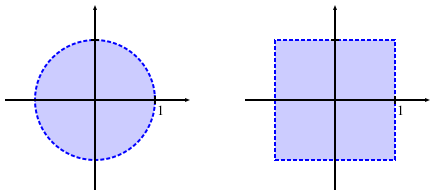
\includegraphics{Equivalence.eps}}
\caption{The open unit balls in $(\R^2, d_E)$ and $(\R^2, d_M)$.}
\label{F:Equivalence}
\end{center}
\end{figure}


\csection{Topological Equivalence}\label{sec_top_equiv}
 
When we can deform one set into another without poking holes in the set, we consider the two sets to be equivalent from a topological perspective. Such a deformation $f$ has to be a bijection to ensure that the two sets contain the same number of elements, continuous so that the inverse images of open sets are open, and $f^{-1}$ must be continuous so images of open sets are open. Such a function provides a one-to-one correspondence between open sets in the two spaces. This leads to the next definition.

\begin{definition} \label{def:MS_topological_equivalence} Two topological spaces $(X,d_X)$ and $(Y,d_Y)$ are \textbf{topologically equivalent}\index{topologically equivalent} if there is a continuous bijection $f : X \to Y$ such that $f^{-1}$ is also continuous.  
\end{definition}

Metric equivalence always implies topological equivalence (using the metric topologies), which is left for Exercise (\ref{ex:me_implies_te}). So metric equivalence is a stronger condition than topological equivalence.

The function $f$ (or $f^{-1}$) in Definition \ref{def:MS_topological_equivalence} is called a \emph{homeomorphism}.

\begin{definition} \label{def:Homeomorphism} Let $(X,\tau_X)$ and $(Y,\tau_Y)$ be topological spaces. A function $f: X \to Y$ is a \textbf{homeomorphism}\index{homeomorphism} if $f$ is a continuous bijection such that $f^{-1}$ is also continuous.  
\end{definition}

If there is a homeomorphism from $(X,\tau_X)$ to $(Y,\tau_Y)$ we say that the spaces $(X,\tau_X)$ to $(Y,\tau_Y)$ are \emph{homeomorphic}\index{homeomorphic spaces} topological spaces. 

It can be difficult to show directly that two metric spaces are homeomorphic, but there are ways to make the process easier in metric spaces. If $f$ is a homeomorphism from the metric space $(\R^2, d_E)$ to the metric space $(\R^2, d_M)$, the continuity of $f$ ensures a smooth deformation from $\R^2$ to $\R^2$. In terms of the metrics, this means that distances cannot get distorted too much -- in fact, the amount distances are distorted should be bounded. In other words, we might expect that there is a constant $K$ so that $d_E(x,y) \leq K d_M(f(x), f(y))$ for any $x, y \in \R^2$. The next theorem tells us that this is a sufficient condition for topological equivalence when we work in the same underlying space. 

\begin{theorem} Let $X$ be a set on which two metrics $d$ and $d'$ are defined. If there exist positive constants $K$ and $K'$ so that 
\begin{align*}
d'(x,y) &\leq K d(x,y) \\
d(x,y) &\leq K' d'(x,y)
\end{align*}
for all $x,y \in X$, then $(X,d)$ is topologically equivalent to $(X,d')$.  
\end{theorem}

\begin{proof} Let $X$ be a set on which two metrics $d$ and $d'$ are defined. Suppose there exist positive constants $K$ and $K'$ so that 
\begin{align*}
d'(x,y) &\leq K d(x,y) \\
d(x,y) &\leq K' d'(x,y)
\end{align*}
for all $x,y \in X$. Let $i_X : (X,d) \to (X,d')$ be the identity mapping. That is, $i_X(x)=x$ for all $x \in X$. We will prove that $i_X$ is a homeomorphism. We know that $i_X$ is a bijection, so we only need verify that $i_X$ and $i_X^{-1}$ are continuous. Let $\epsilon > 0$ be given, and let $a \in X$. Let $\delta = \frac{\epsilon}{K}$. Suppose $x \in X$ so that $d(x,a) < \delta$. Then 
\[d'(i_X(x), i_X(a)) = d'(x,a) \leq Kd(x,a) < K\delta = K\left(\frac{\epsilon}{K}\right) = \epsilon.\]
Thus, $i_X$ is continuous. The same argument shows that $i_X^{-1}$ is also continuous. Therefore, $i_X$ is a homeomorphism between $(X,d)$ and $(X,d')$. 
\end{proof}


\begin{activity} ~
\ba
\item Are $(\R^2,d_T)$ and $(\R^2, d_M)$ topologically equivalent? Explain.

\item Are $(\R^2,d_E)$ and $(\R^2, d_T)$ topologically equivalent? Explain.

\item Do you expect that $(\R^2,d_E)$ and $(\R^2, d_M)$ are topologically equivalent. Explain without doing any calculations or comparisons.

\ea

\end{activity}

\begin{comment}

\ActivitySolution

\ba
\item Let $x = (x_1,x_2)$ and $y=(y_1,y_2)$ be in $\R^2$. Notice that 
\[d_M(x,y) = \max\{| x_1-y_1 |, | x_2-y_2 |\} \leq | x_1-y_1 | + | x_2-y_2 | = d_T(x,y).\]
Also,
\[d_T(x,y) = | x_1-y_1 | + | x_2-y_2 | \leq 2\max\{| x_1-y_1 |, | x_2-y_2 |\} = 2d_M(x,y).\]
So $(\R^2,d_T)$ and $(\R^2, d_M)$ are topologically equivalent. 

\item Let $x = (x_1,x_2)$ and $y=(y_1,y_2)$ be in $\R^2$. Notice that 
\[d_E(x,y) = \sqrt{(x_1-y_1)^2 + (x_2-y_2)^2} \leq \sqrt{(x_1-y_1)^2} + \sqrt{(x_2-y_2)^2} =  | x_1-y_1 | + | x_2-y_2 | \leq d_T(x,y).\]
Also,
\[d_T(x,y) = | x_1-y_1 | + | x_2-y_2 | = \sqrt{(x_1-y_1)^2} + \sqrt{(x_2-y_2)^2} \leq \sqrt{(x_1-y_1)^2+(x_2-y_2)^2} + \sqrt{(x_1-y_1)^2+(x_2-y_2)^2} = 2d_E(x,y).\]
So $(\R^2,d_T)$ and $(\R^2, d_T)$ are topologically equivalent. 

\item If $f: (\R^2,d_T) \to (\R^2, d_M)$ and $g: (\R^2,d_E) \to (\R^2, d_T)$ are homeomorphisms, then we know that $f \circ g$ is a continuous bijection as is $(f \circ g)^{-1}$. So it must be the case that $(\R^2,d_E)$ and $(\R^2, d_M)$ are topologically equivalent. 
 
\ea

\end{comment}


\csection{Relations}\label{sec_relations}
We use the word ``equivalent" deliberately when talking about metric or topological equivalence. Recall that equivalence is a word used with relations, and that a relation is a way to compare two elements from a set. We are familiar with many relations on sets, ``$<$", ``$=$", ``$\geq$" on the integers, for example.  

\begin{definition} A \emph{relation}\index{relation} on a set $S$ is a subset $R$ of $S \times S$.
\end{definition}

For example, the subset $R = \{(a,a) \mid a \in \Z \}$ of $\Z \times \Z$ is the relation we call equals. If $R$ is a relation on a set $S$, we usually suppress the set notation and write $a \sim b$ if $(a,b) \in R$ and say that $a$ is related to $b$. In this case we often refer to $\sim$ as the relation instead of the set $R$. Sometimes we use familiar symbols for special relations. For example, we write $a = b$ if $(a,b) \in R = \{(a,a) \mid a \in \Z \}$.

When discussing relations, there are three specific properties that we consider.

\begin{itemize}
\item A relation $\sim$ on a set $S$ is \emph{reflexive} if $a \sim a$ for all $a \in S$.
\item A relation $\sim$ on a set $S$ is \emph{symmetric} if whenever $a \sim b$ in $S$ we also have $b \sim a$.
\item A relation $\sim$ on a set $S$ is \emph{transitive} if whenever $a \sim b$ and $b \sim c$ in $S$ we also have $a \sim c$.
\end{itemize}

When we use the word ``equivalence", we are referring to an equivalence relation.

\begin{definition} An \textbf{equivalence relation}\index{equivalence relation} is a relation on a set that is reflexive, symmetric, and transitive.  
\end{definition}


\begin{activity} ~
\ba
\item Explain why metric equivalence is an equivalence relation.

\item Explain why topological equivalence is an equivalence relation.

\ea

\end{activity}

\begin{comment}

\ActivitySolution

\ba
\item Let $(X, d_X)$, $(Y, d_Y)$, and $(Z, d_Z)$ be metric spaces. The identity function $id_X : X \to X$ is a bijection that satisfies 
\[d_X(x,y) = d_X(id_X(x), id_X(y)).\]
So $X$ is metrically equivalent to $X$ and metric equivalence is a reflexive relation. 

Suppose that there is a bijection $f: X \to Y$ such that 
\[d_X(x,y) = d_Y(f(x),f(y))\]
for all $x$ and $y$ in $X$. The fact that $f$ is a bijection means that $f^{-1}$ is a bijection from $Y$ to $X$. Let $u$ and $v$ be in $Y$. Then $x = f^{-1}(u)$ and $y = f^{-1}(v)$ are well defined in $X$. Then $f(x) = u$ and $f(y) = v$, and 
\[d_Y(u,v) = d_Y(f(x), f(y)) = d_X(x,y) = d_X(f^{-1}(u), f^{-1}(v)).\]
This makes $(Y, d_Y)$ metrically equivalent to $(X,d_X)$ and metric equivalence is a symmetric relation.

Finally, suppose that there is a bijection $f: X \to Y$ such that 
\[d_X(x,y) = d_Y(f(x),f(y))\]
for all $x$ and $y$ in $X$, and that there is a bijection $g: Y \to Z$ such that 
\[d_Y(u,v) = d_Z(g(u),g(v))\]
for all $u$ and $v$ in $Y$. Let $h = g \circ f$. We know that the composite of bijections is a bijection, so $h: X to Z$ is a bijection. Moreover, if $x$ and $y$ are in $X$, then 
\[d_X(x,y) = d_Y(f(x),f(y)) = d_Z(g(f(x)), g(f(y)) = d_Z(h(x), h(y)).\]
So $X$ is metrically equivalent to $Z$ and metric equivalence is a transitive relation. We conclude that metric equivalence is an equivalence relation. 

\item Let $(X, \tau_X)$, $(Y, \tau_Y)$, and $(Z, \tau_Z)$ be topological spaces. The identity function $id_X : X \to X$ is a continuous bijection whose inverse ($id_X$) is also a continuous bijection. So $X$ is topologically equivalent to $X$ and topological equivalence is a reflexive relation. 

Suppose that there is a continuous bijection $f: X \to Y$ such that $f^{-1}$ is also continuous. Then $f^{-1} : Y \to X$ is a continuous bijection whose inverse is also continuous. This makes $Y$ topologically equivalent to $X$ and topological equivalence is a symmetric relation.

Finally, suppose that there is a continuous bijection $f: X \to Y$ such that $f^{-1}$ is also continuous, and that there is a continuous bijection $g: Y \to Z$ such that $g^{-1}$ is also continuous. Let $h = g \circ f$. We know that the composite of bijections is a bijection, so $h: X to Z$ is a bijection. Moreover, the composite of continuous function is continuous. So $h$ is a continuous bijection from $X$ to $Z$ such that $h^{-1}$ is also continuous. Thus, 
So $X$ is topologically equivalent to $Z$ and topological equivalence is a transitive relation. We conclude that topological equivalence is an equivalence relation. 

\ea


\end{comment}

Equivalence relations are important because an equivalence relation on a set $S$ partitions the set into a disjoint union of equivalence classes. Since topological equivalence is an equivalence relation, we can treat the spaces that are topologically equivalent to each other as being essentially the same space from a topological perspective. Under the relation of homeomorphism we call the equivalence classes \emph{homeomorphism} classes. 


\csection{Topological Invariants}\label{sec_top_invar}
Homeomorphic topological spaces are essentially the same from a topological perspective, and they share many properties, but not all. The properties they share are called \textit{topological invariants} or \emph{topological properties}.

\begin{definition} A property of a topological space $X$ is a \textbf{topological property}\index{topological property} (or \textbf{topological invariant}\index{topological invariant}) if every topological space homeomorphic to $X$ has the same property. 
\end{definition}

\begin{activity} Which of the following are topological invariants? That is for topological spaces $(X, \tau_X)$ and $(Y, \tau_Y)$, if $X$ and $Y$ are homeomorphic space and $X$ has the property, does it follow that $Y$ must also have that property?
\ba
\item $X$ has the indiscrete topology
\item $X$ has the discrete topology
\item $X$ has the finite complement topology
\item $X$ contains the number 2
\item $X$ contains exactly 13 elements
\ea
\end{activity}


\begin{comment}

\ActivitySolution
\ba
\item If $O$ is an open set in $T$, then $f^{-1}(O)$ is open in $X$. This means that $f^{-1}(O)$ is either $\emptyset$ or $X$. It follows that $O$ is either $\emptyset$ or $O = Y$. Thus, having the indiscrete topology is a topological invariant. 

\item Since there is a homeomorphism $f$ from $X$ to $Y$, the image of any open set in $X$ is open in $Y$. The fact that $f$ is an injection means that $\{f(x) \mid x \in X\}$ runs over all single point sets in $Y$, and these sets must be open. So having the discrete topology is a topological property.

\item Let $f$ be a homeomorphism from $X$ to $Y$. Let $O$ be an open set in $Y$.  We know that $f^{-1}(Y \setminus O) = X \setminus f^{-1}(O)$. Since $X \setminus f^{-1}(O)$ is open, the set $X \setminus f^{-1}(O)$ is finite. So $f^{-1}(Y \setminus O)$ is finite. The fact that $f$ is an injection means that $Y \setminus (O)$ is finite.  So every open set $O$ in $Y$ satisfies $Y \setminus O$ is finite. Now we have to prove the converse.

Suppose $B$ is a subset of $Y$ such that $Y \setminus B$ is finite. Then $f^{-1}(Y \setminus B)$ is finite. This implies that $X \setminus f^{-1}(B)$ is finite and so $f^{-1}(B)$ is open in $X$. Since $f^{-1}$ is continuous and $f$ is a bijection, $f(f^{-1}(B)) = B$ is open in $Y$. So having the finite complement topology is a topological property.

\item Containing a specific element is not a topological property. For example, $X = \{1,2\}$ and $Y = \{a,b\}$, both with the discrete topology, are homeomorphic, but $2 \notin Y$. 

\item Since a homeomorphism $f$ is a bijection, the number of elements in a set is preserved under $f$. So the number of elements in a set is a topological invariant.
 
\ea

\end{comment}

\csection{Summary}\label{sec_cont_top_summ}
Important ideas that we discussed in this section include the following.
\begin{itemize}
\item A function $f$ from a topological space $X$ to a topological space $Y$ is continuous if $f^{-1}(O)$ is open in $X$ whenever $O$ is open in $Y$. 
\item Two metric spaces $(X,d_X)$ and $(Y,d_Y)$ are metrically equivalent if there is a bijection $f : X \to Y$ such that 
\begin{align*}
d_X(x,y) &= d_Y(f(x),f(y)) \\
d_Y(u,v) &= d_X(f^{-1}(u), f^{-1}(v))
\end{align*}
for all $x,y \in X$ and $u,v \in Y$. That is, $X$ and $Y$ are metrically equivalent if there is a isometry $f$ from $X$ to $Y$ such that $f^{-1}$ is also an isometry. Topological equivalence is a less stringent condition. Two topological spaces $X$ and $Y$ are topologically equivalent if there is a continuous function $f$ from $X$ to $Y$ such that $f^{-1}$ is also continuous. That is, $X$ and $Y$ are topologically equivalent if there is a homeomorphism between $X$ to $Y$. 
\item A homeomorphism between topological spaces $X$ and $Y$ is a continuous function $f$ from $X$ to $Y$ such that $f^{-1}$ is also continuous. Two topological spaces $X$ and $Y$ are homeomorphic if there is a homeomorphism $f : X \to Y$. 
\item A topological invariant is any property that topological space $X$ has that must also be a property of any topological space homeomorphic to $X$. We can sometimes use topological invariants to determine if two topological spaces are not homeomorphic.
\end{itemize}

\csection{Exercises}\label{sec_cont_top_exer}

\be

\item \label{ex:isometry_reverse} Let $(X,d_X)$ and $(Y,d_Y)$ be metrically equivalent metric spaces, and let $f:X \to Y$ be a bijection such that 
\[d_X(x,y) = d_Y(f(x),f(y))\]
for all $x,y \in X$. Prove that 
\[d_Y(u,v) = d_X(f^{-1}(u), f^{-1}(v))\]
for all $u$ and $v$ in $Y$. 

\begin{comment}

\ExerciseSolution Let $u,v$ be elements in $Y$. Since $f$ is a bijection, there exist $x$ and $y$ in $X$ such that $f(x) = u$ and $f(y) = b$, or $u = f^{-1}(x)$ and $b = f^{-1}(y)$. Then
\[d_Y(u,v) = d_Y(f(x),f(y)) = d_X(x,y) = d_X(f^{-1}(u), f^{-1}(v)).\]

\end{comment}

\item Let $(X, \tau_X)$ and $(Y, \tau_Y)$ be topological spaces, and let $f : X \to Y$ be a homeomorphism. Let $A$ be a subset of $X$.
\ba
\item If $x$ is a limit point of $A$, must $f(x)$ be a limit point of $f(A)$? Prove your answer.

\item If $x$ is an interior point of $A$, must $f(x)$ be an interior point of $f(A)$? Prove your answer.

\item If $x$ is a boundary point of $A$, must $f(x)$ be a boundary point of $f(A)$? Prove your answer.

\ea

\begin{comment}

\ExerciseSolution

\ba
\item Let $x$ be a limit point of $A$ and let $O$ be an open set containing $f(x)$ in $Y$. Since $f$ is continuous, we know that $f^{-1}(O)$ is an open set in $X$ that contains $x$. Thus, $f^{-1}(O)$ contains a point $a$ in $A$ different from $x$. Since $a \in f^{-1}(O)$ we know that $f(a) \in O$. Also, $a \in A$ implies that $f(a) \in f(A)$. The fact that $f$ is a bijection means that $f(a) \neq f(x)$. But then $O$ contains the element $f(a)$ in $f(A)$ that is different from $f(x)$, so $f(x)$ is a limit point of $f(A)$. 

\item Let $x$ be an interior point of $A$. Then there is an open set $O$ with $x \in O \subseteq A$. The fact that $f^{-1}$ is continuous means that $f(O)$ is an open subset of $Y$. Since $O \subseteq A$, we also have $f(x) \in f(O) \subseteq f(A)$. So $f(A)$ is a neighborhood of $f(x)$ and $f(x)$ is an interior point of $f(A)$. 

\item Let $x$ be a boundary point of $A$, and let $O$ be an open set that contains $f(x)$. Since $f$ is continuous, we know that $f^{-1}(O)$ is an open set in $X$ that contains $x$. Thus, $f^{-1}(O)$ contains a point $a$ in $A$ and a point $c$ in $X \setminus A$. Then $f(a) \in f(A)$ and $f(x) \in f(X \setminus A) = Y \setminus f(A)$. Thus, $f(x)$ is a boundary point of $f(A)$. 

\ea


\end{comment}

\item \label{ex:me_implies_te} Let $(X, d_X)$ and $(Y, d_Y)$ be metrically equivalent metric spaces. Show that $X$ and $Y$ are topologically equivalent using the metric topologies. 

\begin{comment}

\ExerciseSolution Let $f : X \to Y$ be a bijection such that $d_X(x,y) = d_Y(f(x),f(y))$ for all $x, y \in X$. To show that $f$ is continuous in the metric topology, we will show that the inverse of any open ball in $Y$ is an open set in $X$. Let $B_Y = B(z,\delta)$ be an open ball in $Y$. Let $B_X = f^{-1}(B_Y)$. We will show that $B_X = B(f^{-1}(z), \delta)$ in $X$, which will verify that the inverse image of $B_Y$ under $f$ is an open set in $X$. 

Let $x \in B_X$. Then $x = f^{-1}(t)$ for some $t \in B_Y$, or $t = f(x)$. It follows that 
\[d_X(x,f^{-1}(z)) = d_Y(f(x),f(f^{-1}(z))) = d_Y(t,z) < \delta.\]
Thus, $x \in B(f^{-1}(z), \delta)$ and $B_X \subseteq B(f^{-1}(z), \delta)$. 

Now let $x \in B(f^{-1}(z), \delta)$. Then $d_X(x, f^{-1}(z)) < \delta$. Let $t = f(x)$. It follows that 
\[d_Y(t,z) = d_X(f^{-1}(t), f^{-1}(z)) = d_X(x, f^{-1}(z)) < \delta.\]
Thus, $t \in B_Y$ and $x \in f^{-1}(B_Y)$ or $x \in B_X$.  This shows that $B(f^{-1}(z), \delta) \subseteq B_X$, which allows us to conclude that $B_X = B(f^{-1}(z), \delta)$. Therefore, $f$ is continuous. The same argument applied to $f^{-1}$ shows that $f^{-1}$ is also continuous. So $X$ and $Y$ are topologically equivalent. 

\end{comment}

\item \label{ex:closed_sets_continuity_TS} Prove theorem \ref{thm:closed_sets_continuity_TS} that if $(X,\tau_X)$ and $(Y, \tau_Y)$ are topological spaces, and $f: X \to Y$ is a function, then $f$ is continuous if and only if $f^{-1}(C)$ is a closed set in $X$ whenever $C$ is a closed set in $Y$. 

\begin{comment}

\ExerciseSolution Assume that $f$ is a continuous function, and let $C$ be a closed set in $Y$. Since $C$ is closed, we know that $Y \setminus C$ is open. The continuity of $f$ means that $f^{-1}(Y \setminus C)$ is also open. Activity \ref{act:CS_1} tell us that $f^{-1}(Y \setminus B) = X \setminus f^{-1}(C)$. The fact that $X \setminus f^{-1}(C)$ is open implies that $f^{-1}(C)$ is closed. 

Now we assume that inverse images of closes sets are closed, and show that $f$ is a continuous function. Let $O$ be an open set in $Y$. Then $Y \setminus O$ is a closed set. Activity \ref{act:CS_1} tells us that $f^{-1}(Y \setminus O) = X \setminus f^{-1}(O)$. That $X \setminus f^{-1}(O)$ is closed means that $f^{-1}(O)$ is open. Thus, $f$ is a continuous function. 

\end{comment}



\item Let $(X, \tau_X)$, $(Y, \tau_Y)$, and $(Z, \tau_Z)$ be topological spaces.
\ba
\item Let $f: X \to Y$ and $g : Y \to Z$ be continuous functions. Prove that $g \circ f : X \to Z$ is a continuous function. (Hint: Exercise (\ref{ex:inverse_composite_sets}) on page \pageref{ex:inverse_composite_sets} could be helpful here.)

\item Let $f: (X, \tau_X) \to (Y, \tau_Y)$ be a homeomorphism. Let $h$ be a function from $(Y, \tau_Y)$ to $(Z, \tau_Z)$ and let $k$ be a function from $(Z, \tau_Z)$ to $(X, \tau_X)$ . 
	\begin{enumerate}[i.]
	\item Prove that $h$ is continuous if and only if $h \circ f$ is continuous. 
	
	\item Prove that $k$ is continuous if and only if $f \circ k$ is continuous. 

	\end{enumerate}
\ea

\begin{comment}

\ExerciseSolution 

\ba

\item  Let $(X, \tau_X)$, $(Y, \tau_Y)$, and $(Z, \tau_Z')$ be topological spaces, and let $f: X \to Y$ and $g : Y \to Z$ be continuous functions. To prove that $g \circ f$ is a continuous function, let $O$ be an open set in $Z$. Since $g$ is continuous, we know that $g^{-1}(O)$ is an open set in $Y$. The fact that $f$ is continuous implies that $f^{-1}(g^{-1}(O))$ is an open set in $X$. Exercise (\ref{ex:inverse_composite_sets}) on page \pageref{ex:inverse_composite_sets} shows that $(g \circ f)^{-1}(O) = f^{-1}(g^{-1}(O))$. We conclude that $(g \circ f)^{-1}(O)$ is an open set in $X$ whenever $O$ is an open set in $Z$. %To demonstrate that $g \circ f$ is continuous, we will prove that $(g \circ f)^{-1}(O) = f^{-1}(g^{-1}(O))$. This will show that $(g \circ f)^{-1}(O)$ is an open set in $X$ whenever $O$ is an open set in $Z$. 

%To prove the set equality $(g \circ f)^{-1}(O) = f^{-1}(g^{-1}(O))$, we verify the containment in both directions. Let $x \in (g \circ f)^{-1}(O)$. Then $(g \circ f)(x) = g(f(x)) \in O$. So $f(x) \in g^{-1}(O)$ and $x \in f^{-1}(g^{-1}(O))$. Thus, $(g \circ f)^{-1}(O) \subseteq  f^{-1}(g^{-1}(O))$. For the reverse containment, let $x \in  f^{-1}(g^{-1}(O))$. Then $f(x) \in g^{-1}(O)$ and $(g \circ f)(x) = g(f(x)) \in O$. Thus, $x \in (g \circ f)^{-1}(O)$ and $f^{-1}(g^{-1}(O)) \subseteq (g \circ f)^{-1}(O)$. The two containments verify that $(g \circ f)^{-1}(O) = f^{-1}(g^{-1}(O))$, and so $g \circ f$ is a continuous function. 

\item
	\begin{enumerate}[i.]
	\item We will demonstrate that $h$ is continuous if and only if $h \circ f$ is continuous. If $h$ is continuous and any composite of continuous functions is continuous, we know that $h \circ f$ is continuous. To prove the reverse implication, assume that $h \circ f$ is continuous. Since $f$ is a homeomorphism, we know that $f^{-1}$ is a continuous function. Part (a) then implies that $(h \circ f)(f^{-1})$ is continuous. But $(h \circ f)(f^{-1}) = h(f \circ f^{-1}) = h$, and so $h$ is continuous. 

	\item We will demonstrate that $k$ is continuous if and only if $f \circ k$ is continuous. If $k$ is continuous, part(a) shows that $f \circ k$ is continuous. To prove the reverse implication, assume that $f \circ k$ is continuous. Since $f$ is a homeomorphism, we know that $f^{-1}$ is a continuous function. Part (a) then implies that $(f^{-1})(f \circ k)$ is continuous. But $(f^{-1})(f \circ k) = (f^{-1}f)k = k$, and so $k$ is continuous. 

	\end{enumerate}

\ea

\end{comment}

\item Let $X = \{a,b,c,d\}$ with topology $\tau = \{\emptyset, \{a\}, \{b\}, \{a,b\}, \{b,d\}, \{a,b,d\}, X\}$. 

\ba

\item Find a function $f: X \to X$ that is continuous at exactly one point, or show that no such function exists.

\item Find a function $f: X \to X$ that is continuous at exactly two points, or show that no such function exists.

\item Find a function $f: X \to X$ that is continuous at exactly three points, or show that no such function exists.

\ea

\begin{comment}

\ExerciseSolution Since the only open set in $X$ that contains $c$ is $X$, any function $f: X \to X$ will be continuous at $c$. 

\ba

\item We are looking for a function that is not continuous at any other point other than $c$.

Let $f: X \to X$ be defined by $f(a) = f(b) = c$, $f(c) = a$, and $f(d) = b$. 
\begin{itemize}
\item Since $f^{-1}(\{a\}) = \{c\}$ is not open in $X$, we notice that $f$ is not continuous at $a$.

\item Since $f^{-1}(\{b\}) = \{d\}$ is not open in $X$, we notice that $f$ is not continuous at $b$.

\item Since $f^{-1}(\{b,d\}) = \{d\}$ is not open in $X$, we notice that $f$ is not continuous at $d$.

\end{itemize}

So $f$ is continuous only at $c$.

\item Let $f: X \to X$ be defined by $f(a) = a$, $f(b) = b$, and $f(c) = d = f(d)$. 
\begin{itemize}
\item Since $f^{-1}(\{a\}) = \{a\}$,  $f^{-1}(\{a,b\}) = \{a,b\}$, and $f^{-1}(\{a,b,d\}) = X$, we notice that $f$ is continuous at $a$.

\item Since $f^{-1}(\{b,d\}) = \{b,c,d\}$ is not open in $X$, we notice that $f$ is not continuous at $b$ or $d$.

\end{itemize}

So $f$ is continuous only at $a$ and $c$.

\item Let $f: X \to X$ be defined by $f(a) = b$, $f(b) = b$, and $f(c) = c$, and $f(d) = a$. 

\begin{itemize}
\item Since $f^{-1}(\{a\}) = \{d\}$, which is not an open set, we notice that $f$ is not continuous at $a$.

\item Since $f^{-1}(\{b\}) = \{a,b\}$,  $f^{-1}(\{a,b\}) = \{a,b,d\}$, $f^{-1}(\{b,d\}) = \{a,b\}$, and $f^{-1}(\{a,b,d\}) = \{a,b,d\}$, we notice that $f$ is continuous at $b$.

\item Since the only open sets that contain $d$ also contain $b$, if $f$ is continuous at $b$ then $f$ is continuous at $d$.

\end{itemize}

So $f$ is continuous only at $b$, $c$, and $d$.


\ea



\end{comment}

\item Consider $\R$ and $\R^2$ equipped with the Euclidean topology. Let $f : \R \to \R$ be a function and let 
\[\Gamma_f = \{(x,f(x)) \mid x \in \R\}\]
be the graph of $f$. Note that $\Gamma_f$ is a subspace of $\R^2$ and is a topological space using the subspace topology. 
	\ba
	\item Show that if $f$ is a continuous function, then $\Gamma_f$ is homeomorphic to $\R$. 
	
	\item If we remove the condition that $f$ is continuous, must it still be the case that $\Gamma_f$ is homeomorphic to $\R$? Prove your conjecture.
	
	\ea

\begin{comment}

\ExerciseSolution
	\ba
	\item Define $g: \R \to \Gamma_f$ by $g(x) = (x,f(x))$. Clearly, $g$ is a surjection. If $x \neq y$ in $\R$, then $(x,f(x)) \neq (y,f(y))$ and so $g$ is also an injection. Note that $g^{-1} : \Gamma_f \to R$ is defied by $g^{-1}((x,f(x)) = x = p_1|_{\Gamma_f}$, the restriction of the projection function to $\Gamma_f$. So $g^{-1}$ is continuous. It remains to show that $g$ is continuous. Recall that a basis for the open sets in $\R^2$ is the set $U \times V$, where $U$ and $V$ are open sets in $\R$. Let $O = \Gamma_f \cap (U \times V)$ for some open sets $U$ and $V$ in $\R$. Then $O =  \{(x,f(x)) \mid x \in U\}$. It follows that $g^{-1}(O) =U$, which is an open set in $\R$.  Since $g$ is a continuous bijection whose inverse is continuous, we conclude that $g$ is a homeomorphism, and that $\Gamma_f$ is homeomorphic to $\R$.  
 
	\item Consider the function $f: \R \to \R$ defined by $f(x) = \begin{cases} 1&\text{ if } x \geq 0 \\ -1 &\text{ if } x < 0.\end{cases}$ Then the graph of $f$ has two connected components, while $\R$ has only one. So $\Gamma_f$ is not homeomorphic to $\R$. 
	
	\ea	
	
\end{comment}	


\item Let $X$ be a nonempty set and let $p$ be a fixed element in $X$. Let $\tau_p$ be the particular point topology and $\tau_{\overline{p}}$ the excluded point topology on $X$. That is
\begin{itemize}
\item $\tau_{p}$ is the collection of subsets of $X$ consisting of $\emptyset$, $X$, and all of the subsets of $X$ that contain $p$.  
\item $\tau_{\overline{p}}$ is the collection of subsets of $X$ consisting of $\emptyset$, $X$, and all of the subsets of $X$ that do not contain $p$.
\end{itemize}
That the particular point and excluded point topologies are topologies is the subject of Exercises (\ref{ex:particular_point_topology}) and (\ref{ex:excluded_point_topology}) on page \pageref{ex:particular_point_topology}. 

	\ba
	\item Let $p$ be a fixed point in $\R$. Is the identity function $i: \R \to \R$ defined by $i(x) = x$ for all $x \in \R$ a homeomorphism from $(\R, \tau_p)$ to $(\R, \tau_{\overline{p}})$? Prove your answer.
	
	\item Is $(\R, \tau_{p})$ homeomorphic to $(\R, \tau_{\overline{p}})$ with the specific point $p=0$? Prove your answer. 

	\ea
	
\begin{comment}

\ExerciseSolution

\ba
\item The answer is no because the inverse image of the open set $\{q\}$, where $q \neq p$ in $(\R, \tau_{\overline{p}})$ is not open in $(\R, \tau_p)$. 

\item Suppose $f$ is a bijection from $(\R, \tau_0)$ to $(\R, \tau_{\overline{0}})$.  We consider the cases $f(0) = 0$ and $f(0) \neq 0$. 
\begin{itemize}
\item Suppose $f(0) = 0$. Let $O = \{1\}$. Since $0 \notin O$, we know that $O$ is an open set in $(\R, \tau_{\overline{0}})$. The fact that $f$ is a bijection, $f^{-1}(O) = \{b\}$, where $b \in \R$ and $f(b) = 1$. The fact that $f(0) = 0$ implies that $b \neq 0$. So $0 \notin f^{-1}(O)$ and $f^{-1}(O)$ is not open. We conclude that $f$ is not a continuous function.
\item Suppose $f(0) \neq 0$. Let $b = f(0)$. Let $c \in \R$ with $c \neq 0$ and $c \neq b$, and let $O = \{c\}$. Since $0 \notin O$, we know that $O$ is an open set in $(\R, \tau_{\overline{0}})$. Then $f^{-1}(O) = \{d\}$ where $d \in \R$ and $f(d) = c$. The fact that $f(0) =b \neq c$ implies that $d \neq 0$. So $0 \notin f^{-1}(O)$ and $f^{-1}(O)$ is not open. We conclude that $f$ is not a continuous function.
\end{itemize}
So there can be no continuous bijection from $(\R, \tau_{p})$ to $(\R, \tau_{\overline{p}})$, we conclude that these two spaces are not homeomorphic. 
\ea

\end{comment}

\item A topological space $X$ is \emph{embedded} in a topological space $Y$ if there is a homeomorphism from $X$ to some subspace of $Y$. The homeomorphism is called an \emph{embedding}.
	\ba
	\item Show that if $X$ is the open interval $(0,1)$ with the Euclidean metric topology, then $X$ can be embedded in the topological space $\R$ with the Euclidean metric topology.
	
	\item  Show that there exist non-homeomorphic topological spaces $A$ and $B$ for which $A$ can be embedded in $B$ and $B$ can be embedded in $A$. 
	
	\ea

\begin{comment}

\ExerciseSolution 

\ba
\item Define $f: X \to \R$ by $f(x) = x$. It is clear that $f$ is a bijection. If $O$ is an open set in $\R$, then $f^{-1}(O) = O \cap (0,1)$, which is a relatively open set. So $f$ is continuous. Now let $U$ be an open subset of $(0,1)$. Then $f(U) = U$, which is open in $\R$. 

\item Let $A = (u,v)$ and $B = (a,b) \cup (c,d)$, with $u<v$ and $a<b<c<d$. We will first show that $A$ can be embedded in $B$ and $B$ can be embedded in $A$.

Define $f: A \to B$ by $f(x) = a + \frac{b-a}{v-u}(x-u)$. Since $f$ is a linear function, we know that $f$ is an injection. Also, $f((u,v)) = (a,b)$, so $f$ maps $A$ into $B$. All that remains is to show that $f$ and $f^{-1}$ are continuous. Note that $f^{-1}(x) = u + \frac{v-u}{b-a}(x-a)$ and so $f$ and $f^{-1}$ are both linear functions. Their continuity was established in Exercise \ref{ex:linear_continuous} on page \pageref{ex:linear_continuous}. Thus, $A$ can be embedded into $B$.

Now define $g: B \to A$ by $g(x) = u + \frac{v-u}{d-a}(x-a)$. As in the previous case, $g$ and $g^{-1}$ are linear functions, and $g$ maps $B$ onto $\left(u,u+\frac{v-u}{d-a}(b-a)\right) \cup \left( u+\frac{v-u}{d-a}(c-a), v\right)$. So $B$ can be embedded into $A$. 

It remains to show that $A$ and $B$ are not homeomorphic spaces. To do so, we will use the following result. \\

\noindent \textbf{Claim:} The only subsets of $A$ that are both open and closed are $\emptyset$ and $A$ itself. \\

\noindent \emph{Proof:} We know that $\emptyset$ and $A$ are both open and closed. It remains to show that these are the only such sets. 

Suppose $P$ is a subset of $A$ that is both open and closed. We will show that $P$ is either empty or all of $A$. 

If $P = \emptyset$, we are done. Suppose $P$ is non-empty. We must show that $P = A$. We proceed by contradiction. Suppose $P \neq A$. Then there is an element $x \in A-P$. Let $P_x$ be the set of all points in $P$ that are greater than $x$, that is $$P_x = \{p \in P \mid p>x\}.$$ Since $x$ is a lower bound for $P_x$, the set $P_x$ has a greatest lower bound. Let $$l = \text{glb}=(P_x).$$ We will show that $l$ is a limit point of $P$. To this end, we will show that every open ball centered at $l$ contains a point of $P$ different from $l$. 

Let $\epsilon$ be greater than 0 and consider the open ball $B(l,\epsilon)$. Suppose $$B(l,\epsilon) \cap P_x = \emptyset.$$ Let $m = \frac{l+\epsilon}{2}$. Then there are no elements of $P_x$ between $l$ and $m$. This makes $m$ a lower bound of $P_x$. But  $m > l$. This contradicts the fact that $l$ is the greatest lower bound for $P_x$. We must therefore have that every open ball around $l$ intersects $P_x$. Since $l$ is not in $P$, $l$ cannot be in $P_x$. So every open ball around $l$ contains a point of $P_x \subset P$ different from $l$. This shows that $l \in P'$, the set of limit points of $P$. Recall that $P$ is closed. This means that $P$ contains its limit points. Thus $l \in P$, a contradiction. Q.E.D. \\

To complete the problem, we must show that $A$ and $B$ cannot be homeomorphic. If there is a homeomorphism $f:A \to B$, then $f$ is continuous. Since $S = (c,d)$ is both open and closed in $B$, then $f^{-1}(S)$ is both open and closed in $A$. Therefore, $f^{-1}(S) = \emptyset$ or $f^{-1}(S) = A$. In the former case, there are no elements in $A$ that map to $S$. In the latter case, everything in $A$ maps to $S$. In neither case would $f$ be a surjection, and thus not a homeomorphism. 

\ea

\end{comment}

\item Let $X = \{a,b\}$ be a two element set. 
\ba

\item Find all of the distinct topologies on $X$. Be sure to explain how you know you have identified all of the topologies. 

\item Determine the distinct homeomorphism classes of topological spaces on two elements. Justify your response.

\ea

\begin{comment}

\ExerciseSolution

\ba

\item The indiscrete topology is $\{\emptyset, X\}$ and the discrete topology is $\{\emptyset, \{a\}, \{b\}, X\}$. The only possibilities for a topology that contains $\{a\}$, is the discrete topology or $\tau_a = \{\emptyset, \{a\}, X\}$. Similarly, the remaining topology on $X$ is $\tau_b = \{\emptyset, \{b\}, X\}$. 

\item Since homeomorphisms preserve open sets, and since the indiscrete topology has only two open sets, none of the other topological spaces are homeomorphic to $X$ with the indiscrete topology. Similarly, the discrete topology is the only topology on $X$ with four open sets, so $X$ with the discrete topology forms its own homeomorphism class. 

We will now show that $(X, \tau_a)$ and $(X, \tau_b)$ are in the same homeomorphism class. Let $f : (X, \tau_1) \to (X, \tau_2)$ by $f(a) = b$ and $f(b) = a$. By definition, $f$ is a bijection. Since $f^{-1}(\emptyset) = \emptyset)$, $f^{-1}(\{b\}) - \{a\}$, and $f^{-1}(X) = X$, we conclude that $f$ is a continuous function. The fact that Since $f(\emptyset) = \emptyset)$, $f(\{a\}) - \{b\}$, and $f(X) = X$ means that $f$ is an open function. We conclude that $f$ is a homeomorphism and that $(X, \tau_1)$ and $(X, \tau_2)$ are in the same homeomorphism class. 

To summarize, the homeomorphism classes of topological spaces $X = \{a, b\}$ with two elements are 
\begin{itemize}
\item $X$ with the indiscrete topology,
\item $(X, \{\emptyset, \{a\}, X\})$,
\item $X$ with the discrete topology.
\end{itemize}


\ea


\end{comment}





\item Let $X = \{a,b,c\}$. There are 29 distinct topologies on $X$, shown below. Determine the number of distinct homeomorphism classes for these 29 topologies and identify the elements of each homeomorphism class. Justify your answers. 

\begin{multicols}{2}
\begin{enumerate}[1.]

\item $\{\emptyset, X\}$

\item $\{\emptyset, \{a,b\}, X\}$

\item $\{\emptyset, \{a,c\}, X\}$

\item $\{\emptyset, \{b,c\}, X\}$

\item $\{\emptyset, \{a\}, X\}$

\item $\{\emptyset, \{b\}, X\}$

\item $\{\emptyset, \{c\}, X\}$

\item $\{\emptyset, \{a\}, \{a,b\}, X\}$

\item $\{\emptyset, \{a\}, \{a,c\}, X\}$

\item $\{\emptyset, \{a\}, \{b,c\}, X\}$

\item $\{\emptyset, \{b\}, \{a,b\}, X\}$

\item $\{\emptyset, \{b\}, \{a,c\}, X\}$

\item $\{\emptyset, \{b\}, \{b,c\}, X\}$

\item $\{\emptyset, \{c\}, \{a,b\}, X\}$

\item $\{\emptyset, \{c\}, \{a,c\}, X\}$

\item $\{\emptyset, \{c\}, \{b,c\}, X\}$

\item $\{\emptyset, \{a\}, \{a,b\}, \{a,c\}, X\}$

\item $\{\emptyset, \{b\}, \{a,b\}, \{b,c\}, X\}$

\item $\{\emptyset, \{c\}, \{a,c\}, \{b,c\}, X\}$

\item $\{\emptyset, \{a\}, \{b\}, \{a,b\}, X\}$

\item $\{\emptyset, \{a\}, \{c\}, \{a,c\}, X\}$

\item $\{\emptyset, \{b\}, \{c\}, \{b,c\}, X\}$

\item $\{\emptyset, \{a\}, \{b\}, \{a,b\}, \{a,c\}, X\}$

\item $\{\emptyset, \{a\}, \{b\}, \{a,b\}, \{b,c\}, X\}$

\item $\{\emptyset, \{a\}, \{c\}, \{a,c\}, \{a,b\}, X\}$

\item $\{\emptyset, \{a\}, \{c\}, \{a,c\}, \{b,c\}, X\}$

\item $\{\emptyset, \{b\}, \{c\}, \{b,c\}, \{a,b\}, X\}$

\item $\{\emptyset, \{b\}, \{c\}, \{b,c\}, \{a,c\}, X\}$

\item the discrete topology

\end{enumerate}

\end{multicols}

\begin{comment}

\ExerciseSolution The only topology on which there are exactly two open sets is the indiscrete topology, so that topology forms its own class. Similarly, the only topology for which all subsets are open is the discrete topology, so that topology forms its own class. We can further sort topologies by counting the types of open sets. If a space has $n$ open sets with $m$ elements, then so does any space homeomorphic to it. This reduces us to consider the following groups:
\begin{description}
\item[Group 1.] $\{\emptyset, \{a,b\}, X\}$,  $\{\emptyset, \{a,c\}, X\}$, and $\{\emptyset, \{b,c\}, X\}$

\item[Group 2.] $\{\emptyset, \{a\}, X\}$, $\{\emptyset, \{b\}, X\}$, and $\{\emptyset, \{c\}, X\}$

\item[Group 3.] $\{\emptyset, \{a\}, \{a,b\}, X\}$, $\{\emptyset, \{a\}, \{a,c\}, X\}$, $\{\emptyset, \{a\}, \{b,c\}, X\}$, $\{\emptyset, \{b\}, \{a,b\}, X\}$, $\{\emptyset, \{b\}, \{a,c\}, X\}$, $\{\emptyset, \{b\}, \{b,c\}, X\}$, $\{\emptyset, \{c\}, \{a,b\}, X\}$, $\{\emptyset, \{c\}, \{a,c\}, X\}$, \\ $\{\emptyset, \{c\}, \{b,c\}, X\}$

\item[Group 4.] $\{\emptyset, \{a\}, \{a,b\}, \{a,c\}, X\}$, $\{\emptyset, \{b\}, \{a,b\}, \{b,c\}, X\}$, $\{\emptyset, \{c\}, \{a,c\}, \{b,c\}, X\}$

\item[Group 5.] $\{\emptyset, \{a\}, \{b\}, \{a,b\}, X\}$, $\{\emptyset, \{a\}, \{c\}, \{a,c\}, X\}$, $\{\emptyset, \{b\}, \{c\}, \{b,c\}, X\}$

\item[Group 6.] $\{\emptyset, \{a\}, \{b\}, \{a,b\}, \{a,c\}, X\}$, $\{\emptyset, \{a\}, \{b\}, \{a,b\}, \{b,c\}, X\}$, \\ $\{\emptyset, \{a\}, \{c\}, \{a,c\}, \{a,b\}, X\}$, $\{\emptyset, \{a\}, \{c\}, \{a,c\}, \{b,c\}, X\}$, \\ $\{\emptyset, \{b\}, \{c\}, \{b,c\}, \{a,b\}, X\}$, $\{\emptyset, \{b\}, \{c\}, \{b,c\}, \{a,c\}, X\}$

\end{description}

We analyze each group. Throughout, let $\{r, s, t\} = X = \{u,v,w\}$ and let $f$ be defined by $f(r) = u$, $f(s) = v$, and $f(t) = w$.
\begin{itemize}
\item In group 1, the function $f$ is a homeomorphism from $(X, \{\emptyset, \{r,s\}, X\})$ to \\ $(X, \{\emptyset, \{u,v\}, X\})$. So all topological spaces in group 1 are homeomorphic. 

\item In group 2, the function $f$ is a homeomorphism from $(X, \{\emptyset, \{r\}, X\})$ to \\ $(X, \{\emptyset, \{u\}, X\})$. So all topological spaces in group 2 are homeomorphic. 

\item If $g: X_1 \to X_2$ is  homeomorphism, then $g$ is one-to-one and so $g(U \cap V) = g(U) \cap g(V)$ for any subsets $U$ and $V$ of $X_1$. So if $U \cap V$ is not empty, then $g(U) \cap g(V)$ is not empty. This splits group 3 into two sets 
\begin{description}
\item[Group 3a.] $\{\emptyset, \{a\}, \{a,b\}, X\}$, $\{\emptyset, \{a\}, \{a,c\}, X\}$, $\{\emptyset, \{b\}, \{a,b\}, X\}$, \\ $\{\emptyset, \{b\}, \{b,c\}, X\}$, $\{\emptyset, \{c\}, \{a,c\}, X\}$, and $\{\emptyset, \{c\}, \{b,c\}, X\}$
\item[Group 3b.] $\{\emptyset, \{a\}, \{b,c\}, X\}$, $\{\emptyset, \{b\}, \{a,c\}, X\}$, and $\{\emptyset, \{c\}, \{a,b\}, X\}$,
\end{description}
where $X$ with any topology in group 3a cannot be homeomorphic to $X$ with any topology in group 3b. 

Regarding the spaces in group 3a, the function $f$ from $(X, \{\emptyset, \{r\}, \{r,s\}, X\})$ to \\ $(X, \{\emptyset, \{u\}, \{u,v\}, X\})$ is a homeomorphism. Thus, $(X, \tau_1)$ and $(X, \tau_2)$ are homeomorphic if $\tau_1$ and $\tau_2$ are any topologies in group 3a. 

Similarly, for group 3b, the function $f$ from $(X, \{\emptyset, \{r\}, \{s,t\}, X\})$ to \\ $(X, \{\emptyset, \{u\}, \{v,w\}, X\})$ is a homeomorphism. Thus, $(X, \tau_1)$ and $(X, \tau_2)$ are homeomorphic if $\tau_1$ and $\tau_2$ are any topologies in group 3b.  

\item The function $f$ from $(X, \{\emptyset, \{r\}, \{r,s\}, \{r,t\},X\})$ to $(X, \{\emptyset, \{u\}, \{u,v\}, \{u,w\}, X\})$ is a homeomorphism. Thus, $(X, \tau_1)$ and $(X, \tau_2)$ are homeomorphic if $\tau_1$ and $\tau_2$ are any topologies in group 4.  

\item The function $f$ from $(X, \{\emptyset, \{r\}, \{s\}, \{r,s\},X\})$ to $(X, \{\emptyset, \{u\}, \{v\}, \{u,v\}, X\})$ is a homeomorphism. Thus, $(X, \tau_1)$ and $(X, \tau_2)$ are homeomorphic if $\tau_1$ and $\tau_2$ are any topologies in group 5.  

\item The function $f$ from $(X, \{\emptyset, \{r\}, \{s\}, \{r,s\}, \{r,t\}, X\})$ to \\ $(X, \{\emptyset, \{u\}, \{v\}, \{u,v\}, \{u,w\}, X\})$ is a homeomorphism. Thus, $(X, \tau_1)$ and $(X, \tau_2)$ are homeomorphic if $\tau_1$ and $\tau_2$ are any topologies in group 6. 

\end{itemize}

This produces 9 homeomorphism classes, one with the indiscrete topology, the group 1 topologies, the group 2 topologies, the group 3a and 3b topologies, the group 4 topologies, the group 5 topologies, the group 6 topologies, and the discrete topology. The topologies for the distinct homeomorphism classes are shown in the table below. 

\begin{multicols}{2}
\begin{enumerate}[1.]

\item $\{\emptyset, X\}$

\item $\{\emptyset, \{a,b\}, X\}$

\item $\{\emptyset, \{a\}, X\}$

\item $\{\emptyset, \{a\}, \{a,b\}, X\}$

\item $\{\emptyset, \{a\}, \{b,c\}, X\}$

\item $\{\emptyset, \{a\}, \{a,b\}, \{a,c\}, X\}$

\item $\{\emptyset, \{a\}, \{b\}, \{a,b\}, X\}$

\item $\{\emptyset, \{a\}, \{b\}, \{a,c\}, \{b,c\}, X\}$

\item the discrete topology

\end{enumerate}

\end{multicols}

\end{comment}

\item Show that property $T_i$ is a topological property for each $i$. (See Section \ref{sec:Closed_sets_topology} for definitions of the separation axioms.) 

\begin{comment}

\ExerciseSolution Let $X$ and $Y$ be homeomorphic topological spaces with $f: X \to Y$ a homeomorphism. We take each case in turn.
	\begin{itemize}
	\item Assume that $X$ is $T_1$. To show that $Y$ is $T_1$, let $y_1$ and $y_2$ be distinct points in $Y$. Since $f$ is a bijection, there are distinct points $x_1, x_2 \in X$ with $f(x_1) = y_1$ and $f(x_2) = y_2$. Since $X$ is $T_1$, there is an open set $O$ in $X$ such that $x_2 \in O$ and $x_1 \notin O$. Since $f$ is an open mapping, the set $U = f(O)$ is open in $Y$. Now $y_2 = f(x_2) \in U$ but $y_1 = f(x_1) \notin U$. Therefore, $Y$ is $T_1$.
	
	\item Assume that $X$ is $T_2$. To show that $Y$ is $T_2$, let $y_1$ and $y_2$ be distinct points in $Y$. Since $f$ is a bijection, there are distinct points $x_1, x_2 \in X$ with $f(x_1) = y_1$ and $f(x_2) = y_2$. Since $X$ is $T_2$, there exist disjoint open sets $O$ and $P$ in $X$ such that $x_1 \in O$ and $x_2 \in P$. Since $f$ is an open mapping, the sets $U = f(O)$ and $V = f(P)$ are open in $Y$. Also, $y_1 = f(x_1) \in U$ and $y_2 = f(x_2) \in V$. It remains to show that $U \cap V = \emptyset$. Suppose to the contrary that there is an element $z$ in $U \cap V$. Then $z= f(r) = f(s)$ for some $r \in O$ and $s \in P$. But $O \cap P = \emptyset$, so $r \neq s$. This violates the fact that $f$ is an injection. We conclude that $Y$ is $T_2$.
	
	\item Assume that $X$ is $T_3$. Then $X$ is also $T_1$, and we have already shown that $Y$ must be $T_1$. To show that $Y$ is $T_3$, we need to demonstrate that $Y$ is regular. Let $D$ be a closed set in $Y$ and let $y \in Y \setminus D$. Let $x \in X$ such that $f(x) = y$, and let $C = f^{-1}(D)$. Since $f$ is continuous, we know that $C$ is a closed set in $X$. The fact that $f(x) \notin D$ means that $x \notin C$. Because $X$ is regular, there exist disjoint open sets $O$ and $P$ in $X$ such that $C \subseteq O$ and $x \in P$. Let $U = f(O)$ and $V = f(P)$. Then $U$ and $V$ are open in $Y$. The fact that $f$ is a bijection means that $f(C) = D$, and the fact that $C \subseteq O$ implies that $D = f(C) \subseteq f(O) = U$. Also, $y = f(x) \in f(P) = V$. That $U$ and $V$ are disjoint is the same argument as in the previous case. We conclude that $Y$ is also $T_3$. 

	\item Assume that $X$ is $T_4$. Then $X$ is also $T_1$, and we have already shown that $Y$ must be $T_1$. To show that $Y$ is $T_4$, we need to demonstrate that $Y$ is normal. Let $H$ and $K$ be disjoint closed sets in $Y$. Let  $C = f^{-1}(H)$ and $D = f^{-1}(K)$. Since $f$ is continuous, we know that $C$ and $D$ closed sets in $X$. Since $X$ is normal there exist disjoint open sets $O$ and $P$ in $X$ such that $C \subseteq O$ and $D \subseteq P$. Let $U = f(O)$ and $V = f(P)$. Then $U$ and $V$ are open in $Y$. The fact that $f$ is a bijection means that $f(C) = H$ and $f(D) = K$. It follows that $H = f(C) \subseteq f(O) = U$ and $K = f(D) \subseteq f(P) = V$. That $U$ and $V$ are disjoint is the same argument as in the previous case. We conclude that $Y$ is also $T_4$. 	
	
	\end{itemize}

\end{comment}

\item For each of the following, answer true if the statement is always true. If the statement is only sometimes true or never true, answer false and provide a concrete example to illustrate that the statement is false. If a statement is true, explain why. 
	\ba
	\item If $f : X \to Y$ is a continuous function between topological spaces $X$ and $Y$, then for every open subset $U$ of $X$, $f(U)$ is open in $Y$.
	
	\item If $\tau_{FC}$ is the finite complement topology, then $f(x) = x^2$ mapping $(\R, \tau_{FC})$ to $(\R, \tau_{FC})$ is continuous.

	\item If $f : X \to Y$ is a bijective function between topological spaces $X$ and $Y$, and for every open subset $U$ of $X$, $f(U)$ is open in $Y$, then $f$ is a homeomorphism. 

	\item If $X$ and $Y$ are topological space with the discrete topologies, and if $f: X \to Y$ is a bijection, then the spaces $X$ and $Y$ are homeomorphic.

\item Let $S$ be a set and let $R_1$ and $R_2$ be equivalence relations on $S$. Then $R = R_1 \cap R_2$ is also an equivalence relation on $S$.
	
	\item Let $S$ be a set and let $R_1$ and $R_2$ be equivalence relations on $S$. Then $R = R_1 \cup R_2$ is also an equivalence relation on $S$.
		
	\ea

\begin{comment}

\ExerciseSolution

\ba

\item This statement is false. Let $(X, \tau_X) = (\{a,b\}, \{\emptyset, \{a\}, X\})$, \\ $(Y, \tau_Y) = (\{r,s,t\}, \{\emptyset, \{r\}, \{s,t\}, Y\})$, and $f: X \to Y$ defined by $f(a)=s$, $f(b) = t$. Since $f^{-1}(\{r\}) = \emptyset$, $f^{-1}(\{s,t\}) = X$, and $f^{-1}(Y) = X$, we see that the inverse image of every open set is open. So $f$ is continuous. However, $f(\{a\}) = \{s\}$ is not an open set. 

	\item  This statement is true. Let $a \in \R$ and let $O$ be an open set that contains $f(a)=a^2$. We know that $\R \setminus O$ is finite. For each $y \in \R$, the definition of $f$ implies that $f^{-1}\{y\})$ contains at most two elements. So the fact that $\R \setminus O$ is finite implies that $f^{-1}(\R \setminus O)$ is also finite. Since $f^{-1}(\R \setminus O) = \R \setminus f^{-1}(O)$, we have that $\R \setminus f^{-1}(O)$ is finite and $f^{-1}(O)$ is open. We conclude that $f$ is continuous. 
	
	\item This statement is false. Let $X = \{a,b\}$ with $\tau_X = \{\emptyset, \{a\}, X\}$ and $Y = \{1,2\}$ with $\tau_Y = \{\emptyset, \{1\}, \{2\}, Y\}$. Define $f: X \to Y$ by $f(a) = 1$, $f(b) = 2$. Then $f(\emptyset) = \emptyset$, $f(X) = Y$, and $f(\{a\}) = \{1\}$, all of which are open in $Y$. But $f^{-1}(\{2\}) = \{b\}$ is not open in $X$, so $f$ is not continuous. 
	
	\item This statement is true. Since every subset of $X$ is open, $f^{-1}(O)$ will be open whenever $O$ is open in $Y$. Similarly, every subset of $Y$ is open so $f(U)$ is open whenever $U$ is open in $X$. It follows that $f$ is a homeomorphism and $X$ is homeomorphic to $Y$. 
	
	\item This statement is false. Let $S = \R$ and let $R_1 = \{(x,y) \mid x \equiv y \pmod{4}\}$ and $R_2 = \{(x,y) \mid x \equiv y \pmod{5}\}$. Then $(6,2)$ and $(2,7)$ are in $R$, but $(6,7)$ is not. 
	
	\item This statement is true. If $s \in S$, then $(s,s) \in R_1$ and $(s,s) \in R_2$, so $(s,s) \in R$. Suppose $(s,t) \in R$. Then $(s,t) \in R_1$ and $(s,t) \in R_2$. The fact that $R_1$ and $R_2$ are symmetric means that $(t,s) \in R_1$ and $(t,s) \in R_2$. So $(t,s) \in R$. Finally, suppose $(r,s)$ and $(s,t)$ are in $R$. Then $(r,s)$ and $(s,t)$ are in both $R_1$ and $R_2$. The transitivity of $R_1$ and $R_2$ implies that $(r,t) \in R_1$ and $(r,t) \in R_2$. So $(r,t) \in R$. Thus, $R$ is an equivalence relation. 

\ea



\end{comment}

\ee  %14
\achapter{15}{Subspaces}\label{chap:subspaces}


\vspace*{-17 pt}
\framebox{
\parbox{\dimexpr\linewidth-3\fboxsep-3\fboxrule}
{\begin{fqs}
\item What is a subspace of a topological space?
\item How do we define the subspace topology?
\item What are relatively open and closed sets?
\item To what kind of spaces is $\R$ with the standard topology homeomorphic?
\end{fqs}}}

\vspace*{13 pt}

\csection{Introduction}\label{sec_sub}

We have seen that a subset $A$ of a metric space $(X,d_X)$ is a subspace of $X$ using the restriction of the metric $d_X$ to $A$. We do not have a metric in general topological spaces, so that approach can't be duplicated. But, we proved that the open sets in a subspace $A$ of a metric space $(X,d_X)$ are exactly the intersections of open sets in $X$ with $A$. That idea can be transferred to topological spaces. 

To make a subspace $A$ of a topological space $(X,\tau)$ into a topological space, we need to define a topology on $A$.

\begin{pa} Let $(X, \tau)$ be a topological space and $A$ a nonempty subset of $X$. It is reasonable to use the open sets in $X$ to define open sets in $A$. More specifically, we might consider a subset $O_A$ of $A$ to be open in $A$ if $O_A$ is the intersection of $A$ with some open set in $X$, as illustrated in Figure \ref{F:Subspace_open}. With this in mind we define $\tau_A$ as 
\[\tau_A = \{O \cap A \mid O \in \tau\}.\]
\begin{figure}[h]
\begin{center}
\resizebox{!}{1.5in}{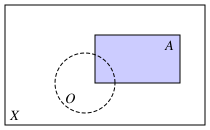
\includegraphics{Subspace_open}}
\caption{A potentially open subset in a subspace.} 
\label{F:Subspace_open}
\end{center}
\end{figure}


\be
\item \label{act:TS_subspace} Show that $\tau_A$ is a topology on $A$.

\vspace{0.1in}

The result of item (1) is that any subset of a topological space $(X,\tau)$ is also a topological space with topology $\tau_A$. 

\begin{definition} \label{def:TS_subspace} Let $(X,\tau)$ be a topological space. A \textbf{subspace}\index{subspace of a topological space} of $(X,\tau)$ is a nonempty subset $A$ of $X$ together with the topology 
\[\tau_A = \{O \cap A \mid O \in \tau\}.\]
\end{definition}

\vspace{0.1in}

\item For each of the following, $X$ is a topological space and $\tau$ is a topology on $X$.
	\ba
	\item Let $X= \{a,b,c,d\}$ and $\tau = \{\emptyset, \{a\}, \{b\}, \{a,b\}, X \}$. Consider the subset $A=\{b,c\}$ and list the open sets in the subspace topology $\tau_A$. Now consider $Z = \{a,b\}$. What is the name of the subspace topology $\tau_Z$ on this subset of $X$?  

	\item  Consider $X=\R$ with $\tau$ the indiscrete topology.  What are the open sets in the subspace topology on $[1,2]$? Now generalize to any nonempty set in the indiscrete topology.

	\item Let $X = \{a,b,c,d,e,f,g,h,i\}$ with $\tau$ the discrete topology. What are the open sets in the subspace topology on $\{a,b,d\}$.  Now generalize to any nonempty set in the discrete topology.

	\item Let $X= \{a,b,c,d,e,f\}$ with $\tau = \{\emptyset,\{a\}, \{c,d\}, \{a,c,d\}, \{b,c,d,e,f\}, X\}$. What are the open sets in the subspace $A = \{a, b, e\}$? Is every open set in $A$ an open set in $X$? Explain.

	\item Let $X=\Z$ with $\tau = \tau_{FC}$ the finite complement topology. What are the open sets in the subspace topology on $A = \{0,19, 37, 5284\}$? Can you generalize this to the subspace topology on any finite subset of $\Z$? 

\item Let $X=\Z$ with $\tau = \tau_{FC}$ the finite complement topology. What are the open sets in the subspace topology on the even integers?  Can you generalize this to the subspace topology on any infinite subset of $\Z$? 

\ea

\ee

\end{pa}


\begin{comment}

\ActivitySolution

\be
\item Since $X \in \tau$ and $X \cap A = A$, we have that $A \in \tau_A$. Also, $\emptyset \in \tau$ and $\emptyset \cap A = \emptyset$. Thus, $\emptyset \in \tau_A$. Now let $U_{\alpha} \in \tau_A$ for all $\alpha$ in some indexing set $I$. For each $\alpha$ there exists $O_{\alpha} \in \tau$ such that $U_{\alpha} = O_{\alpha} \cap A$. Then 
\[\bigcup_{\alpha \in I} U_{\alpha} = \bigcup_{\alpha \in I} A \cap O_{\alpha} = A \cap  \bigcup_{\alpha \in I} O_{\alpha}.\]
But $\bigcup_{\alpha \in I} O_{\alpha} \in \tau$, so it follows that $\bigcup_{\alpha \in I} U_{\alpha} \in \tau_A$. Thus, $\tau_A$ is closed under arbitrary unions. Now let $U_1$, $U_2$, $\ldots$, $U_n$ be in $\tau_A$ for some positive integer $n$. For each $k$ there exists $O_k \in \tau$ such that $U_k = A \cap O_k$. Then
Then 
\[\bigcap_{k=1}^n U_{k} = \bigcap_{k=1}^n A \cap O_{k} = A \cap  \bigcap_{k = 1}^n O_{k}.\]
But $\bigcap_{k=1}^n O_{k} \in \tau$, so it follows that $\bigcap_{k=1}^n U_{k} \in \tau_A$. Thus, $\tau_A$ is closed under finite intersections. We conclude that $\tau_A$ is a topology on $A$. 

\item For each of the following, $X$ is a topological space and $\tau$ is a topology on $X$.
	\ba
	\item  The elements of $\tau_A$ are the intersections of the sets in $\tau$ with $A$. So 
\[\tau_A = \{ \emptyset, \{b\}, A\}.\]
The elements of $\tau_Z$ are the intersections of the sets in $\tau$ with $Z$. So 
\[\tau_Z = \{ \emptyset, \{a\}, \{b\}, \{a,b\}, Z\}.\]
So $\tau_Z$ is the discrete topology on $Z$. 


	\item  The only open sets in the indiscrete topology on a set $X$ are $\emptyset$ and $X$. So if $A$ is a subset of a topological space $X$ with the indiscrete topology, then the induced topology on $A$ is also the indiscrete topology. 


	\item  If $X$ is a topological space with the discrete topology, then every subset of $X$ is open. Thus, if $A$ is a subset of $X$, then $\tau_A = 2^A$. 


	\item  The elements of $\tau_A$ are the intersections of the sets in $\tau$ with $A$. So 
\[\tau_A = \{ \emptyset, \{a\}, \{b,e\}, A\}.\]
The set $\{b,e\}$ is relatively open, but not open in $X$. 

	\item  Recall that the nonempty open sets in $\Z$ are those sets whose complements are finite. Note that the $\Z \setminus \{5\}$ is in $\tau_{FC}$. So if $n \in A$, then $(\Z \setminus \{5\}) \cap \{n\} = \{n\}$. So every subset of $A$ is open and $\tau_{A}$ is the discrete topology. The same argument shows that if $A$ is any finite subset of $\Z$, then the induced topology is the discrete topology. 

\item  Let $\E$ be the set of even integers. We claim that the induced topology is again the finite complement topology. Let $U$ be a subset of $\E$ with $\E \setminus U$ a finite subset of $\E$. Let $O$ be the union of $U$ with the set of odd integers. That is, $O = U \cup (\Z \setminus \E)$. Then $\Z \setminus O = \E \setminus U$ is finite and $O$ is in $\tau_{FC}$. Since $U = \E \cap O$, we have that $U$ is in the subspace topology. Conversely, if $O \in \tau_{FC}$, then $\Z \setminus O$ is finite. Since $\E \subset \Z$, we have $(\E \setminus O) \subseteq (\Z \setminus O)$ and 
\[\E \setminus (\E \cap O) = \E \setminus O\]
 is a finite set. So the only elements in the subspace topology are those whose complements in $\E$ are finite.  
 
 The same argument will show that if $X$ is an infinite topological space with the finite complement topology, then the induced topology on any infinite subset is the finite complement topology. 

\ea

\ee

\end{comment}

\csection{The Subspace Topology}\label{sec_subspace_top}

In our preview activity, we saw that the intersection of the open sets in a topological space $X$ with any nonempty subset $A$ of $X$ forms a topology for $A$. We then have $A$ as a subspace of $X$.  

The topology $\tau_A$ in Definition \ref{def:TS_subspace} is called the \emph{subspace topology}\index{subspace topology}, the \emph{induced topology}\index{induced topology}, or the \emph{relative topology}\index{relative topology}. In our preview activity we saw that sets that are open in a subspace $A$ of a topological space $X$ need not be open in $X$. So we call the sets in $\tau_A$ \emph{relatively open}\index{relatively open set}.  

Once we have defined relatively open sets, we can then consider how to define relatively closed sets. 

\begin{activity} Let $(X, \tau)$ be a topological space, and let $A$ be a subset of $X$.
\ba
\item Recall that a subset of a topological space is closed if its complement is open. Given that $(A, \tau_A)$ is a topological space, how is a closed set in $A$ defined? Such a set will be called \emph{relatively closed}\index{relatively closed set}.

\item Recall that a subset $U$ of $A$ is relatively open if and only if $U = A \cap O$ for some open subset of $X$. With this in mind, how might we expect a relatively closed set in $A$ to be related to a closed set in $X$? State and prove a theorem for this result.  

\ea

\end{activity}

\begin{comment}

\ActivitySolution

\ba
\item A relatively closed set is the complement in $A$ of a relatively open set.

\item
\begin{theorem} Let $(X, \tau)$ be a topological space, and let $A$ be a subset of $X$. A set $C_A \in A$ is relatively closed if and only if $C_A = C \cap A$ for some closed set $C$ in $X$.  
\end{theorem}

\begin{proof} Let $(X, \tau)$ be a topological space, and let $A$ be a subset of $X$. Let $C_A$ be a relatively closed set in $A$. Then $A \setminus C_A$ is a relatively open set in $A$. Thus, $A \setminus C_A = A \cap O$ for some open set $O$ in $X$. Let $C = X \setminus O$. Since $O$ is open in $X$ we know that $C$ is closed in $X$. We will show that $C_A = A \cap C$. Now 
\[C_A = A \setminus (A \setminus C_A) = A \setminus (A \cap O) = A \setminus O = A \cap (X \setminus O) = A \cap C\]
as desired.

For the converse, let $C$ be a closed set in $X$ and suppose $C_A = C \cap A$. To show that $C_A$ is relatively closed, notice that 
\[A \setminus C_A = A \setminus (C \cap A) = A \setminus C = A \cap (X \setminus C).\]
Now $X \setminus C$ is an open set, so $A \setminus C_A$ is a relatively open set. We conclude that $C_A$ is a relatively closed set. 
\end{proof}


\ea

\end{comment}

\csection{Bases for Subspaces}\label{sec_base_sub}

Recall that a basis $\B$ for a topological space is a collection of sets that generate all of the open sets through unions. If we have a basis $\B$ for a topological space $(X, \tau)$, and if $A$ is a subspace of $X$, we might ask if we can find a basis $\B_A$ from $\B$ in a natural way.

\begin{activity} Let $(X, \tau)$ be a topological space with basis $\B$, and let $A$ be a subspace of $X$.
\ba
\item There is a natural candidate to consider as a basis $\B_A$ for $A$. How do you think we should define the elements in $\B_A$?

\item Recall that a set $\B$ is a basis for a topological space $X$ if
\begin{enumerate}
\item For each $x \in X$, there is a set in $\B$ that contains $x$.
\item If $x \in X$ is an element of $B_1 \cap B_2$ for some $B_1, B_2 \in B$, then there is a set $B_3 \in \B$ such that $x \in B_3 \subseteq B_1 \cap B_2$. 
\end{enumerate}
Show that your set from (a) is a basis for the induced topology on $A$.

\ea

\end{activity}

\begin{comment}

\ActivitySolution

\ba
\item It is reasonable to define $\B_A$ as 
\[\B_A = \{B \cap A \mid B \in \B\}.\]

\item Let $a \in A$. Then $a \in X$ so there is a set $B \in \B$ such that $a \in B$. Then $a \in B \cap A$, so $\B_A$ satisfies the first condition of a basis. 

Now suppose $a \in A$ and that $a \in B_1 \cap B_2$ for some $B_1$ and $B_2$ in $\B_A$. By definition of $\B_A$, there are sets $C_1$ and $C_2$ in $\B$ such that $B_1 = A \cap C_1$ and $B_2 = A \cap C_2$. The fact that $\B$ is a basis for $X$ means that there is a set $C_3 \in \B$ such that $a \in C_3 \subseteq C_1 \cap C_2$.   Let $B_3 = A \cap C_3$. Then $a \in B_3$ and 
\[B_3 = A \cap C_3 \subseteq A \cap (C_1 \cap C_2) = (A \cap C_1) \cap (A \cap C_2) = B_1 \cap B_2.\]
It follows that $\B_A$ is a basis for the relative topology on $A$. 

\ea

\end{comment}
 

\csection{Open Intervals and $\R$}\label{sec_open_int_rn}

If we think of a homeomorphism as allowing us to stretch or bend a space, it is reasonable to think that we could stretch an open interval of the form $(a,b)$ infinitely in both directions without altering the nature of the open sets. That is, we should expect that $\R$ with the standard topology is homeomorphic to $(a,b)$ with the subspace topology.   

\begin{activity} Let $a$ and $b$ be real numbers with $a < b$. To show that $(\R, d_E)$ is homeomorphic to $(a,b)$, we need a continuous bijection from $\R$ to $(a,b)$ whose inverse is also continuous. 
\ba
\item First we demonstrate that $(0,1)$ and $\R$ are homeomorphic using the Euclidean metric topology. Let $f : (0,1) \to \R$ be defined by 
\[f(x) = \tan\left(\pi\left(x-\frac{1}{2}\right)\right).\]
	\begin{enumerate}[i.]
	\item Explain why $f$ maps $(0,1)$ to $\R$.
	
	\item Explain why $f$ is an injection.
	
	\item Explain why $f$ is a surjection.
	
	\item Explain why $f$ and $f^{-1}$ are continuous. (Hint: Use a result from calculus.) 
	
	\end{enumerate}

\item The result of (a) is that $\R$ and $(0,1)$ are homeomorphic spaces. To complete the argument that $\R$ is homeomorphic to $(a,b)$, define a function $g: (0,1) \to (a,b)$ and explain why your $g$ is a homeomorphism.

\ea

\end{activity}

\begin{comment}

\ActivitySolution

\ba
\item Let $f(x) = \tan\left(\pi\left(x-\frac{1}{2}\right)\right)$.
	\begin{enumerate}[i.]
	\item Since $\tan(x)$ is defined on $\left(-\frac{\pi}{2}, \frac{\pi}{2}\right)$, we have that $f$ is defined for 
	\[\begin{array}{c}
	-\frac{\pi}{2} < \pi\left(x-\frac{1}{2}\right) < \frac{\pi}{2} \\
	-\frac{1}{2} < x-\frac{1}{2} < \frac{1}{2} \\
	0 < x < 1.
	\end{array}\]
	The output of the tangent function is always a real number, so $f$ maps $(0,1)$ into $\R$. 
	
	\item If $f(a) = f(b)$, then 
	\begin{align*}
	\tan\left(\pi\left(a-\frac{1}{2}\right)\right) &= \tan\left(\pi\left(b-\frac{1}{2}\right)\right) \\
	\tan^{-1}\left(\tan\left(\pi\left(a-\frac{1}{2}\right)\right)\right) &= \tan^{-1}\left(\tan\left(\pi\left(b-\frac{1}{2}\right)\right)\right)  \\
	\pi\left(a-\frac{1}{2}\right) &= \pi\left(b-\frac{1}{2}\right) \\
	a &= b.
	\end{align*}
	Thus, $f$ is an injection. 
	
	\item If $y \in \R$, then 
	\[f\left(\frac{1}{2} + \frac{1}{\pi}\arctan(y)\right) = y,\]
	so $f$ maps $(0,1)$ onto $\R$.
	
	\item Results from calculus apply to $\R$ using the standard metric. Since $f$ is a composite of differentiable functions, we know that $f$ is continuous. Note also that $f$ is invertible with 
	\[f^{-1}(x) = \frac{1}{2} + \frac{1}{\pi}\arctan(x).\]
	We see that $f^{-1}$ is also a differentiable function, therefore continuous. We conclude that $\R$ is homeomorphic to $(0,1)$. 
	 	
	\end{enumerate}

\item Define $g: (0,1) \to (a,b)$ by $g(x) = a+(b-a)x$. As a linear function we know that $g$ is continuous. The fact that $a < b$ implies that $g$ is increasing and invertible. Since $a+(b-a)(0) = a$ and $a+(b-a)(1) = b$, the increasing continuous nature of $g$ shows that $g$ maps $(0,1)$ onto $(a,b)$. The inverse of $g$ is also linear, so $g^{-1}$ is continuous. We conclude that $g$ is a homeomorphism. The transitivity of begin homeomorphic shows that $\R$ is homeomorphic to any open interval of the form $(a,b)$. 

\ea

\end{comment}

It is left to Exercise (\ref{ex:R_intervals}) to show that $\R$ is also homeomorphic to any interval of the form $(a,\infty)$ or $(-\infty,b)$. Later we will determine if $\R$ is homeomorphic to intervals of the form $[a,b)$, $(a,b]$, $[a, \infty)$ or $(-\infty, b]$. 


\csection{Summary}\label{sec_sub_summ}
Important ideas that we discussed in this section include the following.
\begin{itemize}
\item A subspace of a topological space is any nonempty subset of the topological space endowed with the subspace topology. 
\item An open subset in the subspace topology for a subset $A$ of a topological space $X$ is any set of the form $O \cap A$, where $O$ is an open set in $X$. 
\item The relatively open sets are the open sets in a subspace topology. The relatively closed sets are complements of the relatively open sets in a subspace topology. That is, a relatively closed set in the subspace $A$ of a topological space $X$ are the sets of the form $A \cap C$, where $C$ is a closed set in $X$.  
\item The topological space $\R$ with the standard topology is homeomorphic to any open interval as well as open intervals of the form $(a,\infty)$ or $(-\infty,b)$ for any real numbers $a$ and $b$. 
\end{itemize}

\csection{Exercises}\label{sec_sub_exer}

\be


\item Let $X$ and $Y$ be topological spaces and $f: X \to Y$ be a continuous function. If $A$ is a subspace of $X$, prove that $f|_A : A \to Y$ is also continuous.

\begin{comment}

\ExerciseSolution Let $A$ be a subspace of $X$. To show that $f|_A$ is continuous, let $O$ be an open subset of $Y$. Then $f^{-1}(O)$ is open in $X$. So $f^{-1}(O) \cap A$ is open in $A$. We will demonstrate that $f^{-1}(O) \cap A = (f|_A)^{-1}(O)$, which will show that $f|_A$ is continuous. 

Let $x \in f^{-1}(O) \cap A$. Then $x \in f^{-1}(O)$ and $x \in A$. Since $f(x) \in O$ and $x \in A$, it follows that $f|_A(x) \in O$ and $x \in (f|_A)^{-1}(O)$. So $f^{-1}(O) \cap A \subseteq (f|_A)^{-1}(O)$.

Now let $x \in (f|_A)^{-1}(O)$. Then $x$ must be in $A$ and $f|_A(x) \in O$. So $f(x) \in O$ and $x \in f^{-1}(O) \cap A$. We conclude that $(f|_A)^{-1}(O) \subseteq f^{-1}(O) \cap A$ and, consequently, that $f^{-1}(O) \cap A = (f|_A)^{-1}(O)$.

\end{comment}

\item Let $X$ be a topological space, let $A$ be a subspace of $X$, and let $B$ be a subspace of $A$. Show that the subspace topology that $B$ inherits from $A$ is the same as the subspace topology that $B$ inherits from $X$.

\begin{comment}

\ExerciseSolution Let $O$ be an open set in $B$ considered as a subspace of $A$. Then $O = B \cap O_A$ for some set $O_A$ that is open in $A$. Since $O_A$ is open in $A$, there exists an open set $O_X$ in $X$ such that $O_A = A \cap O_X$. But then $O = B \cap O_A = B \cap (A \cap O_X) = B \cap O_X$. So every open set in $B$ as a subspace of $A$ has the form $B \cap O_X$ for some open set $O_X$ in $X$. 

Similarly, if $O_X$ is an open set in $X$, then $A \cap O_X$ is an open set in the subspace $A$. From this it follows that $B \cap (A \cap O_X) = B \cap O_X$ is an open set in $B$ considered as a subspace of $A$. So the subspace topology that $B$ inherits from $A$ is the same as the subspace topology that $B$ inherits from $X$.


\end{comment}

\item Let $A$ be a subspace of a topological space $X$ and let $B$ be a subset of $A$.

\ba

\item Prove that a point $x$ in $A$ is a limit point of $B$ in the subspace topology for $A$ if and only if $x$ is a limit point of $B$ in the topology on $X$.

\item Prove that the closure of $B$ in the subspace topology for $A$ is equal to $\overline{B} \cap A$, where $\overline{B}$ is the closure of $B$ in $X$.

\ea

\begin{comment}

\ExerciseSolution

\ba

\item Suppose $x$ is a limit point of $B$ in the subspace topology for $A$. To show that $x$ is a limit point of $B$ in $X$, let $N$ be a neighborhood of $x$ in $X$. Then $N$ contains an open set $O$ that contains $x$. It follows that $O \cap A$ is a neighborhood of $x$ in $A$. Since $x$ is a limit point of $B$ in $A$, the set $O \cap A$ must contain a point in $B$ different fro $x$. But then $N$ contains a point in $B$ different from $x$ and so $x$ is a limit point of $B$ in $X$.

Conversely, suppose that $x$ is a limit point of $B$ in $X$. To show that $x$ is a limit point of $B$ in $A$, let $N$ be a neighborhood of $x$ in $A$. Then $N$ contains an open set $O$ in $A$ that contains $x$. Since $O$ is open in $A$, there exists an open set $U$ in $X$ such that $O = U \cap A$. But then $U$ is a neighborhood of $x$ in $X$ and so must contain a point in $B$ different from $x$. It follows that $O$ contains a point in $B$ different from $x$, and so does $N$. Therefore, $x$ is a limit point of $B$ in the subspace topology for $A$.

\item The closure of $B$ in $A$ is equal to $B \cup B''$, where $B''$ is the set of limit points of $B$ in $A$, while $\overline{B} = B \cup B'$. So to prove the equality we want, we only need to demonstrate that $B'' = B'$. Part (a) shows exactly this equality. 

\ea

\end{comment}

\item \label{ex:R_intervals} Show that $\R$ is homeomorphic, with the standard topology, to any interval of the form $(a,\infty)$ or $(-\infty,b)$.

\begin{comment}

\ExerciseSolution Let $a \in \R$ and let $f: \R \to (a, \infty)$ be defined by $f(x) = a+e^x$. To show that $f$ is a surjection, let $y \in (a,\infty)$. Then $y = a + z$ for some positive real number $z$. So $f(\ln(z)) = a+e^{\ln(z)} = a+z = a + (y-a) = y$. 

To verify that $f$ is an injection, suppose that $f(x_1) = f(x_2)$ for some real numbers $x_1$ and $x_2$. Then $a+e^{x_1} = a+e^{x_2}$ or $e^{x_1} = e^{x_2}$. Applying the natural log to both sides shows that $x_1 = x_2$. 

Now we need to verify that $f$ and $f^{-1}$ are continuous. Let $(r,s)$ be a basic open set in $\R$. The fact that the exponential function is increasing means that $f((r,s)) = \left(a+e^r, a+e^s\right)$, which is an open set. Thus, $f^{-1}$ is continuous. Now let $(r,s)$ be a basic open set in $(a, \infty)$. Note that $f^{-1}(x) = \ln(x-a)$. The fact that the natural log is increasing shows that $f^{-1}((r,s)) =  (\ln(r-a), \ln(s-a))$ which is an open set. Thus, $f$ is continuous. It follows that $f$ is a homeomorphism and $\R$ is homeomorphic to $(a,\infty)$. 

A similar argument shows that if $b \in \R$, then $g: \R \to (-\infty, b)$ defined by $g(x) = b-e^{x}$ is a homeomorphism. 

\end{comment}

\item Let $X$ be a topological space.
\ba

\item Let $O$ be an open subset of $X$. Prove that a subset $A$ of $O$ is open in $O$ if and only if $A$ is open in $X$. 

\item Let $C$ be a closed subset of $X$. Prove that a subset $B$ of $C$ is closed in $C$ if and only if $B$ is closed in $X$. 

\ea

\begin{comment}

\ExerciseSolution

\ba

\item Let $O$ be an open subset of $X$. Let $A$ be an open subset of $O$. Then there is an open set $U$ in $X$ such that $A = U \cap O$. As the intersection of two open subsets, we conclude that $A$ is open in $X$.

Conversely, let $A$ be a subset of $O$ that is open in $X$. Since $A$ is open in $X$, the set $A \cap O = A$ is open in $A$. 

\item Let $C$ be a closed subset of $X$. Let $B$ be a closed subset of $C$. Then there is a closed set $V$ in $X$ such that $B = V \cap C$. As the intersection of two closed subsets, we conclude that $B$ is closed in $X$.

Conversely, let $B$ be a subset of $C$ that is closed in $X$. Since $B$ is closed in $X$, the set $B \cap C = B$ is closed in $C$. 

\ea

\end{comment}


\item A property of a topological space is said to be hereditary if that property is inherited by every subspace. We state this more  formally in the following definition.

\begin{definition} A property $P$ of a topological space $X$ is \textbf{hereditary}\index{hereditary property} if every subspace of $X$ also has property $P$.
\end{definition}

Show that properties $T_1$, $T_2$, and $T_3$ are hereditary. (The separation axioms $T_i$ are found on page \pageref{sec:Closed_sets_topology}.) The fact that $T_4$ is not hereditary is somewhat difficult. One example is the Tychonoff plank (which is normal) with the Deleted Tychonoff plank (which is not normal) as subspace. An interested reader can consult \emph{Counterexamples in Topology (2nd ed.)}, Lynn Arthur Steen and J. Arthur Seebach, Jr., Dover Publications, 1978.

\begin{comment}

\ExerciseSolution \item Let $X$ be a topological space and $Y$ a subspace of $X$. We consider each property in turn.

	\begin{itemize}
	
	\item Suppose that $X$ is $T_1$. To show that $Y$ is $T_1$, let $y_1$ and $y_2$ be distinct points in $Y$. Then $y_1$ and $y_2$ are distinct points in $X$. The fact that $X$ is $T_1$ implies that there is an open set $O$ in $X$ that contains $y_2$ but not $y_1$. The set $U = O \cap Y$ is open in $Y$ and $y_2 \in U$ but $y_1 \notin U$. We conclude that $Y$ is also $T_1$.
	
	\item This is done in Exercise \ref{ex:Closed_sets:Hausdorff_subspace} on page \pageref{ex:Closed_sets:Hausdorff_subspace}.
	
	\item Suppose that $X$ is $T_3$. Then $X$ is $T_1$ and part (a) shows that $Y$ is $T_1$. So we need to show that $Y$ is regular (this argument also shows that being regular is hereditary). Let $C$ be a closed subset of $Y$ and let $y \in Y \setminus C$. There is a closed subset $D$ of $X$ such that $C = D \cap Y$. Since $y \notin C$ and $y \in Y$, it follows that $y \notin D$. So there exists an open set $O$ in $X$ such that $D \subseteq O$ and $y \notin O$. Let $U = O \cap Y$. Then $U$ is open in $Y$ and 
	\[C = D \cap Y \subseteq O \cap Y = U.\]
Finally, $y \notin O$ so $y \notin U$. We conclude that $Y$ is $T_3$.  
	
	
	\end{itemize}

\end{comment}

\item Suppose that $f : X \to Y$ is a homeomorphism from a topological space $X$ to a topological space $Y$. Let $a \in X$. Must the subspace $X' = X \setminus \{a\}$ of $X$ be homeomorphic to the subspace $Y' = Y \setminus \{f(a)\}$ of $Y$? Prove your conjecture. 

\begin{comment}

\ExerciseSolution The answer is yes. Assume that $f : X \to Y$ is a homeomorphism from a topological space $X$ to a topological space $Y$. Let $a \in X$, and let $X' = X \setminus \{a\}$ and $Y' = Y \setminus \{f(a)\}$. Define $g$ by $g(x) = f(x)$ for all $x \in X'$. Note that the fact that $f$ is an injection shows that $g(x) \neq f(a)$ for any $x \in X'$. Thus, $g : X' \to Y'$. We will prove that $g$ is a homeomorphism, which will imply that $X'$ and $Y'$ are homeomorphic spaces. First we show that $g$ is an injection. 

Let $x_1, x_2 \in X'$ such that $g(x_1) = g(x_2)$. Then $f(x_1) = f(x_2)$. The fact that $f$ is an injection means that $x_1 = x_2$ and so $g$ is an injection. Next we demonstrate that $g$ is a surjection.

Let $y \in Y'$. The fact that $f$ is a surjection implies that there is an $x \in X$ such that $f(x) = y$. Now $y \neq f(a)$, so the fact that $f$ is an injection means that $x \neq a$. Thus, $x \in X'$ and $g$ is a surjection. So $g$ is a bijection from $X'$ to $Y'$. 

Now we need to prove that $g$ and $g^{-1}$ are homeomorphisms. Since $g^{-1}$ is defined by $g^{-1}(y) = f^{-1}(y)$ for all $y \in Y'$, the same argument will work for either $g$ or $g^{-1}$. We demonstrate that $g$ is continuous. Let $O'$ be an open set in $Y'$. Then $O' = O \cap Y'$ for some open set $O$ in $Y$. We know that $f$ is continuous, so $f^{-1}(O)$ is an open set in $X$. Thus, $f^{-1}(O) \cap X'$ is an open set in $X'$. All that remains to do is show that $g^{-1}(O') = f^{-1}(O) \cap X'$. 

Let $x \in g^{-1}(O')$. Then $g(x) \in O' \subseteq O$ and $g(x) \neq f(a)$. Thus, $x \in f^{-1}(O) \cap X'$. Now let $x \in f^{-1}(O) \cap X'$. Then $x \in X'$ and $f(x) = g(x) \in O$. But $x \in X'$ implies $x \neq a$ and so $f(x) = g(x) \in Y'$. So $g(x) \in O \cap Y' = O'$ and so $x \in g^{-1}(O')$. Thus, $g^{-1}(O')$ is an open set in $X$ and $g$ is a continuous function. 

\end{comment}



\item For each of the following, answer true if the statement is always true. If the statement is only sometimes true or never true, answer false and provide a concrete example to illustrate that the statement is false. If a statement is true, explain why. 
	\ba
	\item If $X$ has the discrete topology, then every subspace of $X$ has the discrete topology. 
		
	\item If $X$ is a topological space that does not have the discrete topology, then no subspace of $X$ has the discrete topology.

	\item If $f : X \to Y$ is a continuous function between topological spaces $X$ and $Y$, and $X$ is Hausdorff, then the subspace $f(X)$ of $Y$ is Hausdorff.

	\item If $A$ is a subspace of a topological space $X$ and $B$ is a subset of $X$, then the closure of $B \cap A$ in the subspace topology for $A$ equals $\overline{B} \cap A$, where $\overline{B}$ is the closure of $B$ in $X$. 
	
	\item If $A$ is a subspace of a topological space $X$ and $C$ is a subset of $X$, then the interior of $C \cap A$ in the subspace topology for $A$ equals $\Int(C) \cap A$, where $\Int(C)$ is the interior of $C$ in $X$. 
		
	\ea

\begin{comment}

\ExerciseSolution

\ba

\item This statement is true. Let $A$ be a subset of $X$ and let $B$ be a subset of $A$. Since $A$ is open in $X$, then $A \cap B = B$ is open in $A$. So every subset of $A$ is open and $A$ has the discrete topology. 
		
	\item This statement is false. Let $X = \{a,b,c\}$ with topology $\tau = \{\emptyset, \{a\}, \{b\}, \{a,b\}, X\}$. The subspace topology of the subset $A = \{a,b\}$ of $X$ is the discrete topology. 

\item This statement is false. Let $X = \{a,b,c\}$ with $\tau_X$ the discrete metric, and let $Y = \{a,b,c\}$ with $\tau_Y = \{\emptyset, \{a,b\}, Y\}$. Note that any topological space with the discrete metric is Hausdorff since we can separate points $x$ and $y$ by the open sets $\{x\}$ and $\{y\}$. Let $f : X \to Y$ be the identity map. The inverse image of any open set in $Y$ is open in $X$, so $f$ is continuous. However, $f(X) = Y$ is not Hausdorff because there are no disjoint open sets that separate $a$ and $b$. 

	\item This statement is false. Let $X = \R$ and let $A = \Z$. Let $B$ be the set of irrationals in $X$. Then $A \cap B = \emptyset$ and so the closure of $A \cap B$ in $A$ is empty. Every rational number is a limit of a sequence of irrational numbers, so $\overline{B} = \R$. But this makes $\overline{B} \cap A = A$. 
	
	\item This statement is false. Let $X = \R$ and let $A = \Z$. Let $B$ be the set of rationals in $X$. Then $A \cap B = A$. The subspace topology on $A$ is the discrete topology, so the interior of $A \cap B$ in $A$ is $A$. Every open interval that contains a rational number also contains an irrational number. So $\Int(B) = \emptyset$. But this makes $\Int(B) \cap A = \emptyset$. 	
	
\ea


\end{comment}

\ee
  %15
\achapter{16}{Quotient Spaces}\label{chap:quotients}


\vspace*{-17 pt}
\framebox{
\parbox{\dimexpr\linewidth-3\fboxsep-3\fboxrule}
{\begin{fqs}
\item What is a quotient topology?
\item What is a quotient space?
\item What are two examples of familiar quotient spaces?
\end{fqs}}}

\vspace*{13 pt}

\csection{Introduction}\label{sec_quotients}

We are familiar with the word \emph{quotient} when working with rational numbers. That is, the fraction $\frac{1}{2}$ is the quotient of $1$ by $2$, and the set of rational numbers is the collection of all defined quotients of integers. The word quotient seems to have come from the latin word ``quotiens", which can be translated as ``how often" or ``how many times". We can think of the fraction $\frac{1}{2}$ as dividing a unit ($1)$ into two pieces. So we often apply the word quotient to any kind of construction that divides a set into pieces. Another familiar quotient construction is the set $\Z_n$, the set of quotients of integers after we divide by $n$. Another way to think of $\Z_n$ is as a quotient $\Z/n\Z$, where $n\Z$ is the set of multiples of $n$ and two integers $a$ and $b$ are equal if $b-a \in n\Z$. This defines the relation of congruence module $n$ on $\Z$, and the elements of $\Z/n\Z$ are the equivalence classes for this relation. We make similar constructions in many branches of mathematics by defining an equivalence relation on a set, and we then divide the set into pieces (the equivalence classes) and call the set of equivalence classes a \emph{quotient space}. We explore the concept of quotient spaces of topological spaces in this section.

As an example, take the interval $X = [0,1]$ in $\R$ and bend it to be able to glue the endpoints together. The resulting object is a circle. By identifying the endpoints $0$ and $1$ of the interval, we are able to create a new topological space. We can view this gluing or identifying of points in the space $X$ in a formal way that allows us to recognize the resulting space as a quotient space. 

\csection{The Quotient Topology}\label{sec_quotient_top}

Given a topological space $X$ and a surjection $f$ from $X$ to a set $Y$, we can use the topology on $X$ to define a topology on $Y$. This topology on $Y$ identifies points in $X$ through the function $f$. The resulting topology on $Y$ is called a \emph{quotient} topology. The quotient topology gives us a way of creating a topological space which models gluing and collapsing parts of a topological space.

\begin{pa} Let $X = \{1,2,3,4,5,6\}$ and let $\tau = \{\emptyset, \{1,2\},\{4,6\}, \{1,2,4,6\},X\}$. Let $Y = \{a,b,c,d\}$ and define $p: X \to Y$ by 
\[p(1) = b, \ p(2) = a, \ p(3) = c, \ p(4) = d, \ p(5) = c, \ \text{ and } \ p(6) = a.\] 
Our goal in this activity is to define a topology on $Y$ that is related to the topology on $X$ via $p$. 
\be
\item We know the sets in $X$ that are open. So let us consider the sets $U$ in $Y$ such that $p^{-1}(U)$ is open in $X$. Define $\sigma$ to be this set. That is
\[\sigma = \{U \subseteq Y \mid p^{-1}(U) \in \tau\}.\]
Find all of the sets in $\sigma$. 

\item Show that $\sigma$ is a topology on $Y$.

\item Explain why $p : (X, \tau) \to (Y, \sigma)$ is continuous.

\item Show that $\sigma$ is the largest topology on $Y$ for which $p$ is continuous. That is, if $\sigma'$ is a topology on $Y$ with $\sigma \subsetneqq \sigma'$, then $p: (X,\tau) \to (Y, \sigma')$ is not continuous.

\ee

\end{pa}

\begin{comment}

\ActivitySolution

\be
\item The only possibilities for sets $U$ are those with $p^{-1}(U)$ being $\emptyset$, $\{1,2\}$, $\{4,6\}$, $\{1,2,4,6\}$, and $X$. Since $p$ is a surjection, the only time $p^{-1}(U) = \emptyset$ is when $U = \emptyset$. Also, $p^{-1}(U) = X$ when $X = Y$. We consider the remaining cases in turn. 

\begin{itemize}
\item Since $p(1) = p(6) = b$ and $p(2) = a$, $p^{-1}(U)$ can never be  $\{1,2\}$.
\item Since $p(4) = d$, and $p(2) = p(6) = a$, $p^{-1}(U)$ can never be $\{4,6\}$. 
\item Since $p(1) = b$, $p(2) = p(6) = a$, and $p(4) = d$, $p^{-1}(U) = \{1,2,4,6\}$ when $U = \{a,b,d\}$. 
\end{itemize}
Thus, 
\[\sigma = \{\emptyset, \{a,b,d\}, Y\}.\]

\item By inspection we can see that unions and intersections of sets in $\sigma$ remain in $\sigma$, so $\sigma$ is a topology on $Y$.  

\item By definition, if $U$ is in $\sigma$, then $p^{-1}(U)$ is in $\tau$. So the inverse image of any open set is open under $p$ and $p$ is continuous.

\item Suppose $\sigma'$ is a topology on $Y$ with $\sigma \subset \sigma'$. Then there exists $O \in \sigma' \setminus \sigma$. If $p^{-1}(O)$ were open, then we would have $O \in \sigma$ be definition. But this is a contradiction. So $p^{-1}(O)$ is not open and $p$ is not continuous from $(X \tau)$ to $(Y, \sigma')$. 

\ea

\end{comment}

\csection{Quotient Spaces}\label{sec_quotient_space}

As we saw in our preview activity, if we have a surjection $p$ from a topological space $(X,\tau)$ to a set $Y$, we were able to define a topology on $Y$ by making the open sets the sets $U \subseteq Y$ such that $p^{-1}(U)$ is open in $X$. This is how we will create what is called the \emph{quotient topology}.  Before we can define the quotient topology, we need to know that this construction always makes a topology.

\begin{activity} \label{act:quot_topology} Let $(X,\tau_X)$ be a topological space, let $Y$ be a set, and let $p: X \to Y$ be a surjection. Let 
\[\tau_Y = \{U \subseteq Y \mid p^{-1}(U) \in \tau_X\}.\]
\ba
\item Why are $\emptyset$ and $Y$ in $\tau_Y$?

\item Let $\left\{U_{\beta}\right\}$ be a collection of sets in $\tau_Y$ for $\beta$ in some indexing set $J$. 
	\begin{enumerate}[i.]
	\item Show that $\bigcup_{\beta \in J} U_{\beta}$ is in $\tau_Y$.
	
	\item If $J$ is finite, show that $\bigcap_{\beta \in J} U_{\beta}$ is in $\tau_Y$.
	
	\end{enumerate}
	
\item What conclusion can we draw about $\tau_Y$? 

\ea

\end{activity}

\begin{comment}

\ActivitySolution

\ba
\item Since $p^{-1}(\emptyset) = \emptyset \in \tau_X$ we have that $\emptyset \in \tau_Y$. The fact that $p$ is a surjection means that $p^{-1}(Y) = X \in \tau_X$. So $Y \in \tau_Y$.

\item Let $\left\{U_{\beta}\right\}$ be a collection of sets in $\tau_Y$ for $\beta$ in some indexing set $J$. 
	\begin{enumerate}[i.]
	\item By definition, $p^{-1}(U_{\beta} \in \tau_X$ for every $\beta \in J$. Since $p^{-1}\left(\bigcup_{\beta \in J} U_{\beta}\right) = \bigcup_{\beta \in J} p^{-1}\left(U_{\alpha}\right)$ is in $\tau_X$ it follows that $\bigcup_{\beta \in J} U_{\beta}$ is in $\tau_Y$.
	
	\item Since $p^{-1}\left(\bigcap_{\beta \in J} U_{\beta}\right) = \bigcap_{\beta \in J} p^{-1}\left(U_{\alpha}\right)$ is in $\tau_X$ it follows that $\bigcap_{\beta \in J} U_{\beta}$ is in $\tau_Y$.
	
	\end{enumerate}
	
\item We can conclude that $\tau_Y$ is a topology on $Y$. 

\ea

\end{comment}

Activity \ref{act:quot_topology} allows us to define the quotient topology.

\begin{definition} Let $(X,\tau_X)$ be a topological space, let $Y$ be a set, and let $p: X \to Y$ be a surjection. 
\begin{enumerate}
\item The \textbf{quotient topology}\index{quotient topology} on $Y$ is the set
\[\{U \subseteq Y \mid p^{-1}(U) \in \tau_X\}.\]
\item Any function $p: X \to Y$ is a \textbf{quotient map}\index{quotient map} if $p$ is surjective and for $U \subseteq Y$,  $U$ is open in $Y$ if and only if $p^{-1}(U)$ is open in $X$. 
\item If $p: X \to Y$ is a quotient map, then the space $Y$ is the \textbf{quotient space}\index{quotient space} of $X$ determined by $p$. 
\end{enumerate}
\end{definition}


\begin{activity} ~
\ba
\item Let $X=\R$ with standard topology, let $Y=\{-1,0,1\}$, and define $p:X \to Y$ by 
\[p(x) = \begin{cases} 1&\text{if } x>0 \\ 0 &\text{if } x=0 \\ -1 &\text{if } x<0. \end{cases}\]
Find all of the open sets in the quotient topology. 

\item Let $X=\R$ with standard topology, let $Y=[0,1)$, and define $p:X \to Y$ by 
\[p(x) = x-\lfloor x\rfloor,\]
where $\lfloor x\rfloor$ is the largest integer less than or equal to $x$, (For example $\lfloor 1.2 \rfloor = 1$, and so $p(1.2) = 1.2 - 1 = 0.2$. The function defined by $\lfloor x\rfloor$ is also called the \emph{floor} function. Be careful, note that $\lfloor -0.7 \rfloor = -1$.)  Determine the sets in the quotient topology.  (Hint: The graph of $p$ on $[-2,2]$ is shown in Figure \ref{F:floor}.)
\begin{figure}[h]
\begin{center}
\resizebox{!}{1.0in}{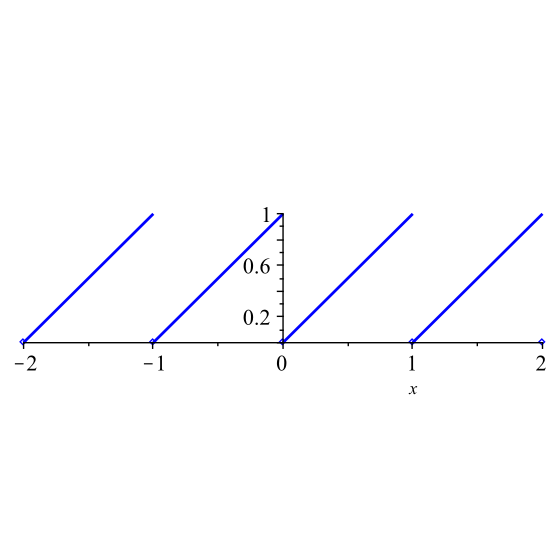
\includegraphics[trim=0.75cm 6.5cm 0.75cm 6.75cm, clip]{floor.eps}}
\caption{The graph of $p(x) = x - \lfloor x\rfloor$.} 
\label{F:floor}
\end{center}
\end{figure}
%\includegraphics[trim=left bottom right top, clip]{file}


\ea

\end{activity}

\begin{comment}

\ActivitySolution
\ba
\item We know that $\emptyset$ and $Y$ are open. We consider all of the remaining subsets of $Y$. Note that 
\begin{align*}
p^{-1}(\{-1\}) &= (-\infty, 0), \\
p^{-1}(\{0\}) &= \{0\}, \\
p^{-1}(\{1\}) &= (0,\infty, 0), \\
p^{-1}(\{-1,0\}) &= (-\infty, 0], \\
p^{-1}(\{-1,1\}) &= (-\infty, 0) \cup (0, \infty), \text{ and } \\
p^{-1}(\{0,1\}) &= [0,\infty).
\end{align*}
The only subsets of $Y$ that have open inverse images are $\{-1\}$, $\{1\}$, and $\{-1,1\}$. So the quotient topology is
\[\{\emptyset, \{-1\}, \{1\}, \{-1,1\}, Y\}.\]

\item The graph shows that for $y$ in $Y$, we have 
\[p^{-1}(y) = \{k+y \mid k \in \Z\}.\]
So $p^{-1}(B) = \{k+b \mid k \in \Z \text{ and } b \in B\}$. The only way for $p^{-1}(B)$ to be open in $X$ is for $p^{-1}(B)$ to be a union of open intervals. This will happen only when $B$ is a union of open intervals in $Y$. Since $p^{-1}((a,b)) = \bigcup_{k \in \Z} (k+a, k+b)$ when $0 \leq a < b < 1$, the quotient topology is 
\[\{\emptyset,Y\} \cup \{(a,b) \mid 0 \leq a < b < 1\}.\]


\ea

\end{comment}

Another perspective of the quotient topology utilizes the fact that any equivalence relation on a set $X$ partitions $X$ into a union of disjoint equivalence classes $[x] = \{y \in X \mid y \sim x\}$. There is a natural surjection $q$ from $X$ to the space of equivalence classes given by $q(x) = [x]$. We investigate this perspective in the next activity.

\begin{activity} \label{act:quotient_er} Let $X = \{a,b,c,d,e,f\}$ and let $\tau = \{\emptyset, \{a\}, \{b\}, \{a, b\}, \{a, b, c\}, \{a, b, c, d\}, X\}$. Then $(X, \tau)$ is a topological space. Let $A = \{a, b, c\}$ and $B = \{d,e,f\}$. Define a relation $\sim$ on $X$ such that $x \sim y$ if $x$ and $y$ are both in $A$ or both in $B$. Assume that $\sim$ is an equivalence relation. The sets $A$ and $B$ are the equivalence classes for this relation. That is $A = [a] = [b] = [c]$ and $B = [d] = [e] = [f]$. Let $X^* = \{A,B\}$. Then we can define $p : X \to X^*$ by sending $x \in X$ to the set to which it belongs. That is, $p(x) = [x]$ for $x \in X$, or 
\[p(a) = A, p(b) = A, p(c) = A, p(d) = B, p(e) = B, \text{ and } p(f) = B.\]
Determine the sets in the quotient topology on $X^*$. 
\end{activity}

\begin{comment}

\ActivitySolution Since $X^{*} = \{A,B\}$, there are only limited possibilities for open sets. We consider each in turn: 
\begin{align*}
p^{-1}(\emptyset) &= \emptyset \\
p^{-1}(\{A\}) &= \{a,b,c\} \\
p^{-1}(\{B\}) &= \{d,e,f\} \\
p^{-1}(X^{*}) &= X.
\end{align*}
From this list we see that the quotient topology on $X^{*}$ is $\{\emptyset, \{A\}, X^{*}\}$. 

\end{comment}

The partition of $X$ in Activity \ref{act:quotient_er} into the disjoint union of sets $A$ and $B$ defines an equivalence relation on $X$ where $x \sim y$ if $x$ and $y$ are both in the same set $A$ or $B$. That is, $a \sim b \sim c$ and $d \sim e \sim f$. In this context, the sets $A$ and $B$ are equivalence classes -- $A = [a]$ and $B = [d]$, where $[x]$ is the equivalence class of $x$. This leads to a general construction.

If $(X, \tau)$ is a topological space and $\sim$ is an equivalence relation on $X$, we can let $X/\ssim$ be the set of distinct equivalence classes of $X$ under $\sim$. Then $p: X \to X/\ssim$ defined by $p(x) = [x]$ is a surjection and $X/\ssim$ has the quotient topology. The space $X/\ssim$ is called a \emph{quotient space}\index{quotient space}. The space $X/\ssim$ is also called an \emph{identification} space\index{identification space} because the equivalence relation identifies points in the set to be thought of as the same. This allows us to visualize quotient spaces as resulting from gluing or collapsing parts of the space $X$.

\begin{figure}[h]
\begin{center}
\resizebox{!}{0.75in}{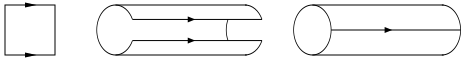
\includegraphics{Cylinder_identification.eps}} 
\caption{A tube as the identification space $X/\ssim$.} 
\label{F:Quotient_tube}
\end{center}
\end{figure}
%\includegraphics[trim=left bottom right top, clip]{file}

\begin{example} Let $I = [0,1]$ and let $X = I \times I$ with standard topology. Define a relation $\sim$ on $X$ by $(x,y) \sim (x,y)$ if $0 < y < 1$ and $0 \leq x \leq 1$, $(x,0) \sim (x,1)$ if $0 \leq x \leq 1$. It is straightforward to show that $\sim$ is an equivalence relation. Let us consider what the identification space $X/\ssim$ looks like. The space $I \times I$ is the unit square as shown in Figure \ref{F:Quotient_tube}. All points in the interior of the square are identified only with themselves. However, the top side and bottom side are identified with each other in the same direction. Think of $X$ as a piece of paper. We roll up the sides of the square to make the top and bottom sides coincide. The result is that $X/\ssim$ is the cylinder as shown in Figure \ref{F:Quotient_tube}. 

\end{example}

\begin{activity} Quotient spaces can be difficult to describe. This activity presents a few more examples. 
\ba
\item Let $X = [0, 1]$ with standard topology and define an equivalence relation $\sim$ on $X$ by $0 \sim 1$ and $x \sim x$ for all $x$ not equal to $0$ or $1$. What does the quotient space $X/\ssim$ look like? (Hint: Think about the relation $\sim$ as gluing the points $0$ and $1$ together.)

\begin{figure}[h]
\begin{center}
\resizebox{!}{1.0in}{\includegraphics{Mobius_identification.eps}} \hspace{0.5in} \resizebox{!}{1.0in}{\includegraphics{Torus_identification.eps}} \hspace{0.5in} \resizebox{!}{1.0in}{\includegraphics[trim=1.8cm 4.0cm 1.25cm 4.7cm, clip]{Quotient_sphere_1.png}} 
\caption{From left to right: the identifications for parts i., ii., and iii.} 
\label{F:Quotients_activity}
\end{center}
\end{figure}

\item Describe quotient spaces of $X = I \times I$ with standard topology given by the following equivalence relations $\sim$. Depictions of the identifications are shown in Figure \ref{F:Quotients_activity}. (Here $I$ is the closed interval $[0,1]$.)
	\begin{enumerate}[i.]
	\item $(x, y) \sim (x,y)$ if $0 < y < 1$ and $0 \leq x \leq 1$ and $(x,0) \sim (1-x,0)$ when $0 \leq x \leq 1$. 
	
	\item $(x, y) \sim (x,y)$ if $0 < x < 1$ and $0 < y < 1$, $(x,0) \sim (x,1)$ for $0 < x < 1$, $(0,y) \sim (1,y)$ for $0 < y < 1$, and $(0,0) \sim (0,1) \sim (1,0) \sim(1,1)$
	
	\item  $(x, y) \sim (x,y)$ if $0 < x < 1$ and $0 < y < 1$ and $(x,y) \sim (u,v)$ if $(x,y)$ and $(u,v)$ are boundary points.
	
	\end{enumerate}
	
\ea

\end{activity}

\begin{comment}

\ActivitySolution

\ba
\item If we take the unit interval $X$ and glue the points $0$ and $1$ together, we obtain a circle, that is the space $S^1$. 

\item Describe quotient spaces of $X = I \times I$ with standard topology given by the following equivalence relations $\sim$. (Here $I$ is the closed interval $[0,1]$.)
	\begin{enumerate}[i.]	
	\item All points in the interior of the square are identified only with themselves. However, the top side and bottom side are identified with each other -- but in the opposite direction as indicated at left in Figure \ref{F:Quotient_Mobius}. So if we roll up and twist the square to make the top and bottom sides coincide in the opposite direction, we obtain the M\"{o}bius strip as shown at right in Figure \ref{F:Quotient_Mobius}.
\begin{figure}[h]
\begin{center}
\resizebox{!}{1.25in}{\includegraphics{Mobius_identification.eps}} \hspace{0.75in} \resizebox{!}{1.25in}{\includegraphics[trim=10.75cm 9.05cm 9.9cm 16.25cm, clip]{Mobius.png}} 
\caption{A M\"{o}bius strip as the identification space $X/\ssim$.} 
\label{F:Quotient_Mobius}
\end{center}
\end{figure}
%\includegraphics[trim=left bottom right top, clip]{file}	

	
	\item All points in the interior of the square are identified only with themselves. However, the left side and right side are identified with each other, as are the top and bottom -- both in the same direction as indicated in Figure \ref{F:Quotient_tube}. So if we first roll up the square to identify the left and right sides, we obtain a cylinder. The top and bottom of the square become the top and bottom of the cylinder. Now bend the cylinder around to identify the top and bottom, resulting in the torus as shown at right in Figure \ref{F:Quotient_torus} (image copied from \url{http://i.stack.imgur.com/FJaFe.png}). . 
\begin{figure}[h]
\begin{center}
\resizebox{!}{0.75in}{\includegraphics{Quotient_torus_2.pdf}} 
\caption{A torus as the identification space $X/\ssim$.} 
\label{F:Quotient_torus}
\end{center}
\end{figure}
%\includegraphics[trim=left bottom right top, clip]{file}	

	\item  All points in the interior of the square are identified only with themselves, but the boundaries points are all identified together as indicated at left in Figure \ref{F:Quotient_sphere}. So the boundary collapses to a point. Think of taking the square and pinching all of the sides together. What is left looks like a sphere, with the sides all identified with a single point on the sphere as shown at right in Figure \ref{F:Quotient_sphere}. %Note: An illustration of this can be seen at \url{https://upload.wikimedia.org/wikipedia/commons/4/44/Disk_to_Sphere_using_Quotient_Space.gif}.
\begin{figure}[h]
\begin{center}
\resizebox{!}{1.25in}{\includegraphics[trim=1.8cm 4.0cm 1.25cm 4.7cm, clip]{Quotient_sphere_1.png}} \hspace{0.75in} \resizebox{!}{1.25in}{\includegraphics[trim=3.2cm 2.3cm 3.0cm 3.1cm, clip]{Quotient_sphere_2.png}} 
\caption{A sphere as the identification space $X/\ssim$.} 
\label{F:Quotient_sphere}
\end{center}
\end{figure}
%\includegraphics[trim=left bottom right top, clip]{file}	

	\end{enumerate}
	
\ea

\end{comment}

Many other interesting identification spaces can be made. For example, let $X = I \times I$ and define $\sim$ by $(x, y) \sim (x,y)$ if $0 < x < 1$ and $0 < y < 1$, $(0, y) \sim (1, y)$ for $0 < y < 1$, $(x,0) \sim (1-x,1)$ for $0 < x < 1$. This identification is illustrated in Figure \ref{F:Klein_bottle}. The resulting identification space $X/\ssim$ is a Klein bottle. A nice illustration of this can be seen at 
\url{https://plus.maths.org/content/introducing-klein-bottle}.
\begin{figure}[h]
\begin{center}
\resizebox{!}{1.25in}{\includegraphics{Klein_identification.eps}} 
\caption{Identifications for the Klein Bottle.} 
\label{F:Klein_bottle}
\end{center}
\end{figure}

\csection{Identifying Quotient Spaces}\label{sec_find_quotient_space}

Suppose $X$ is a topological space and $Y$ is a set, and let $p: X \to Y$ be a surjection. We can define a relation $\sim_p$ on $X$ by $x \sim_P y$ if and only if $p(x) = p(y)$. It is straightforward to show that $\sim_p$ is an equivalence relation. From this we can see that our two approaches to defining the quotient topology and quotient spaces are really the same. 

Oftentimes we have a topological space $X$ and a relation $\sim$ on $X$, and we would like to have an effective way to be able to identify the quotient space $X/\ssim$ as homeomorphic to some familiar topological space $Y$. That is, we want to be able to show that there is a homeomorphism $f$ from $X/\ssim$ to $Y$. 

\begin{example} \label{exp:R_Z_quotient} Consider the following situation. Let $X = \R$ with the standard topology and define the relation $\sim$ on $\R$ by $x \sim y$ if $x - y \in \Z$. It is straightforward to show that $\sim$ is an equivalence relation. By this equivalence relation, we have $x-1 \sim x$ for every real number $x$. This identifies $\R$ with the interval $[0,1]$, where $0$ and $1$ are identified under the relation. So we might expect that $\R/\ssim$ is homeomorphic to the circle $S^1 = \{(x,y) \in \R^2 \mid x^2+y^2 = 1\}$ as a subspace of $\R^2$ with the standard topology. Now the objective is to find a homeomorphism between $S_1$ and $\R/\ssim$. Since every point on the unit circle has the form $(\cos(t), \sin(t))$ for some real number $t$, we might try defining $f: (\R/\ssim) \to S^1$ by $f([t]) = (\cos(t), \sin(t))$. However, we have that $0 \sim 1$, which means that $[0] = [1]$, but $f([0]) \neq f([1])$ and so $f$ is not well-defined. Another option might be $f([t]) = (\cos(2 \pi t), \sin(2 \pi t))$. In this case, if $x \sim y$, then $2 \pi x$ and $2 \pi y$ differ by a multiple of $2 \pi$ and so $f([x]) = f([y])$. We could then show that $f$ is a homeomorphism. We will continue this example shortly.

\end{example}

The following theorem encapsulates the above example.

\begin{theorem} \label{thm:quotient_1} Let $X$ and $Y$ be sets and let $\sim$ be an equivalence relation on $X$. Let $f$ be a function from $X$ to $Y$ such that $f(x_1) = f(x_2)$ whenever $x_1 \sim x_2$ in $X$. Let $X/\ssim$ be the set of equivalence classes of $X$ under the relation $\sim$, and let $p: X \to (X/\ssim)$ be the standard map defined by $p(x) = [x]$.  The function $\overline{f}$ mapping $X/\ssim$ to $Y$ defined by $\overline{f}([x]) = f(x)$ for every $x \in X$ is the unique function that satisfies 
\[f = \overline{f} \circ p.\]
\end{theorem}


\begin{activity} Theorem \ref{thm:quotient_1} is a statement about sets and functions, and there is no topology involved. We prove the theorem in this activity. Use the conditions stated in Theorem \ref{thm:quotient_1}.
\ba
\item Show that $\overline{f}$ is well-defined. That is, show that whenever $[x_1] = [x_2]$ in $X/\ssim$, then $\overline{f}([x_1]) =\overline{f}([x_2])$.

\item Prove that $f = \overline{f} \circ p$. 

\item Show that the uniqueness of $\overline{f}$ comes from the equation $f = \overline{f} \circ p$.

\ea

\end{activity}

\begin{comment}

\ActivitySolution

\ba
\item The fact that $f(x_1) = f(x_2)$ whenever $x_1 \sim x_2$ in $X$ makes $\overline{f}$ well-defined. That is, if $[x_1] = [x_2]$ in $X/\ssim$, then $x_1 \sim x_2$ and so 
\[\overline{f}([x_1]) = f(x_1) = f(x_2) = \overline{f}([x_2]).\]

\item To demonstrate that $f = \overline{f} \circ p$, let $x \in  X$. Then 
\[(\overline{f} \circ p)(x) = \overline{f}(p(x)) = \overline{f}([x]) = f(x).\]

\item For uniqueness, if $g : (X/\ssim) \to Y$ satisfies $g \circ p = f$, then $g(p(x)) = g([x]) = f(x)$ for every $x \in X$ and $g = \overline{f}$.

\ea

\end{comment}

Now we present a final result that can be very helpful when working with quotient spaces.

\begin{theorem} \label{thm:quotient_2} Let $X$ be a topological space and let $\sim$ be an equivalence relation on $X$. Consider the set $X/\ssim$ to be a topological space with the quotient topology, and let $p: X \to (X/\ssim)$ be the standard surjection defined by $p(x) = [x]$. Let $Y$ be a topological space with $f: X \to Y$ a continuous function such that $f(x_1) = f(x_2)$ whenever $x_1 \sim x_2$ in $X$. Then $\overline{f} : (X/\ssim) \to Y$ defined by $\overline{f}([x]) = f(x)$ is the unique continuous function satisfying $f = \overline{f} \circ p$.
\end{theorem}

\begin{proof} The existence of $\overline{f}$ as the unique function satisfying $f = \overline{f} \circ p$ was established in Theorem \ref{thm:quotient_1}. All that remains is to show that $\overline{f}$ is continuous. Let $O$ be an open set in $Y$. Since $f$ is continuous, we know that $f^{-1}(O)$ is open in $X$. If $x_1 \in f^{-1}(O)$ and $x_1 \sim x_2$, then $x_2 \in f^{-1}(O)$ as well. Thus, we can write $f^{-1}(O)$ as
\[f^{-1}(O) = \bigcup_{x \in f^{-1}(O)} [x].\]
That is, $f^{-1}(O)$ is a union of equivalence classes. Now $\overline{f}([x]) = f(x)$, so if $x \in f^{-1}(O)$, then $[x] \in \overline{f}^{-1}(O)$. Thus,
\[f^{-1}(O) = \bigcup_{x \in f^{-1}(O)} [x] = \bigcup_{[x] \in \overline{f}^{-1}(O)} [x] = \overline{f}^{-1}(O).\]
We conclude that $\overline{f}^{-1}(O)$ is open in $X$ and $\overline{f}$ is continuous. 
\end{proof}

Now we will see how to use Theorem \ref{thm:quotient_2} to establish a homeomorphism from a quotient space of a given topological space to another topological space

\begin{example} We return to the situation from Example \ref{exp:R_Z_quotient} with $X = \R$ under the standard topology and equivalence relation $\sim$ defined by $x \sim y$ if $x - y \in \Z$. We will use Theorem \ref{thm:quotient_2} to show that $\R/\ssim$ is homeomorphic to the circle $Y = S^1$. 

\begin{figure}[h]
\begin{center}
\resizebox{!}{1.5in}{\includegraphics{S_1_basis.eps}} 
\caption{A basis element for $S^1$.} 
\label{F:S_1_basis}
\end{center}
\end{figure}
%\includegraphics[trim=left bottom right top, clip]{file}


\begin{description}
\item[Step 1.] Define a continuous surjection $f: X \to Y$ that respects the relation. That is, we need to ensure that $f(x_1) = f(x_2)$ whenever $x_1 \sim x_2$ in $X$. We saw earlier that the function $f$ defined by $f(t) = (\cos(2 \pi t), \sin(2 \pi t))$ respects the relation. Since every point on the unit circle is of the form $(\cos(\theta), \sin(\theta))$ for some real number $\theta$, choosing $t = \frac{\theta}{2 \pi}$ makes $f(t) = (\cos(\theta), \sin(\theta))$ and $f$ is a surjection. Now we need to demonstrate that $f$ is continuous. A collection of basic open sets in $S^1$ can be found by intersecting $S^1$ with open balls in $\R^2$ as illustrated in Figure \ref{F:S_1_basis}. We can see that the basic open sets are arcs of the form $\wideparen{ab}$ for $a$ and $b$ in $S^1$. Suppose $a = (\cos(2 \pi A), \sin(2 \pi A))$ and $b = (\cos(2 \pi B), \sin(2 \pi B))$ for angles $A$ and $B$. Then $f^{-1}(\wideparen{ab})$ is the union of intervals $(A+2\pi k, B+2 \pi k)$ for $k \in \Z$. As a union of open intervals, we have that $f^{-1}(\wideparen{ab})$ is open in $X$. We have now found a continuous surjection from $X$ to $Y$ that respects the relation. 

\item[Step 2.] Find a continuous function from $X/\ssim$ to $Y$. Theorem \ref{thm:quotient_2} tells us that the function $\overline{f} : (X/\ssim) \to Y$ defined by $\overline{f}([t]) = f(t)$ is continuous. So $\overline{f}$ is our candidate to be a homeomorphism. 

\item[Step 3.] Show that $\overline{f}$ is a bijection. Let $y \in Y$. The fact that $f$ is a surjection means that there is a $t \in \R$ such that $f(t) = y$. It follows that $\overline{f}([t]) = f(t) = y$ and $\overline{f}$ is a surjection. To demonstrate that $\overline{f}$ is an injection, suppose $\overline{f}([s]) = \overline{f}([t])$ for some $s, t \in \R$.  Then $(\cos(2 \pi s), \sin(2 \pi s)) = f(s) = f(t) = (\cos(2\pi t), \sin(2 \pi t))$. It must be the case then that $2 \pi s$ and $2 \pi t$ differ by a multiple of $2 \pi$. That is, $2 \pi s - 2 \pi t = 2 \pi k$ for some integer $k$. From this we have $s - t = k \in \Z$, and so $s \sim t$. This makes $[s] = [t]$ and we conclude that $\overline{f}$ is an injection. 

\item[Step 4.] Show that $\overline{f}$ is a homeomorphism. At this point we already know that $\overline{f}$ is a continuous bijection, so the only item that remains is to show that $\overline{f}(\overline{O})$ is open whenever $\overline{O}$ is open in $X/\ssim$. Let $p: X \to (X/\ssim)$ be the standard map. Let $\overline{O}$ be a nonempty open set in $X/\ssim$. Then $O = p^{-1}(\overline{O})$ is open in $X$. Thus, $O$ is a union of open intervals. Let $(a,b)$ be an interval contained in $O$. From the definition of $f$ we have that $f(a,b)$ is the open arc $\wideparen{f(a)f(b)}$, which is open in $Y$. So $f(O)$ is a union of open arcs in $Y$, which makes $f(O)$ open in $Y$. Now $f(O) = (\overline{f} \circ p)(O) = \overline{f}(p(O)) = \overline{f}(\overline{O})$, and $\overline{f}(\overline{O})$ is open in $Y$. We conclude that $\overline{f}$ is a homeomorphism from $X/\ssim$ to $S^1$, and so $S^1$ is a quotient space of $\R$. 
\end{description}

\end{example}





\csection{Summary}\label{sec_quotients_summ}
Important ideas that we discussed in this section include the following.
\begin{itemize}
\item Let $(X,\tau_X)$ be a topological space, let $Y$ be a set, and let $p: X \to Y$ be a surjection. The quotient topology on $Y$ is the set
\[\{U \subseteq Y \mid p^{-1}(U) \in \tau_X\}.\]
\item The function $p$ is a quotient topology as in the previous bullet is called a quotient map and the space $Y$ is a quotient space. 
\item A circle, a M\"{o}bius strip, a torus, and a sphere can all be realized as quotient spaces. 
\end{itemize}

\csection{Exercises}\label{sec_quotients_exer}

\be

\item Let $X$ be the real numbers with the standard topology and let $p: X \to \{a,b,c\}$ be defined by 
\[p(x) = \begin{cases} a &\text{ if } x < 0 \\ b &\text{ if } x = 0 \\ c &\text{ if } x > 0. \end{cases}\]
What is the quotient topology? 

\begin{comment}

\ExerciseSolution A subset $U$ of $\{a,b,c\}$ is in the quotient topology if and only if $p^{-1}(U)$ is open in $X$. Now 
\begin{align*}
p^{-1}(\{a\}) &= (-\infty, 0) \\
p^{-1}(\{b\}) &= \{0\} \\
p^{-1}(\{c\}) &= (0, \infty) \\
p^{-1}(\{a,b\}) &= (-\infty, 0] \\
p^{-1}(\{a,c\}) &= (-\infty, 0) \cup (0, \infty) \\
p^{-1}(\{b,c\}) &= [0,\infty),
\end{align*}
so the quotient topology is $\{\emptyset, \{a\}, \{c\}, \{a,c\}, \{a,b,c\}\}$.  

\end{comment}

\item Define an equivalence relation $\sim$ on $\R^2$ by $(x_1,y_1) \sim (x_2,y_2)$ whenever $x_2 - x_1 \in \Z$ and $y_2 - y_1 \in \Z$. 

\ba

\item Prove that $\sim$ is an equivalence relation on $\R^2$.

\item The quotient space is a familiar space. Find that space and explain why it is the quotient space.

\ea

\begin{comment}

\ExerciseSolution 

\ba

\item Let $(x_1,y_1)$, $(x_2, y_2)$, and $(x_3,y_3)$ be in $\R^2$. Since $x_1 - x_1 = 0 = y_1 - y_1$ we see that $(x_1,y_1) \sim (x_1, y_1)$ and $\sim$ is reflexive.

Now suppose that $(x_1,y_1) \sim (x_2,y_2)$. Then $x_2 - x_1 \in \Z$ and $y_2 - y_1 \in \Z$. So $x_1 - x_2 = -(x_2-x_1) \in \Z$ and $y_1-y_2 = -(y_2 - y_1) \in \Z$. Thus, $(x_2, y_2) \sim (x_1,y_1)$ and $\sim$ is symmetric.

Finally, suppose that $(x_1,y_1) \sim (x_2,y_2)$ and $(x_2,y_2) \sim (x_3,y_3)$. Then $x_3-x_1 = (x_3-x_2) + (x_2-x_1) \in \Z$ and $(y_3-y_1) = (y_3-y_2) + (y_2-y_1) \in \Z$ and $\sim$ is transitive. Therefore, $\sim$ is an equivalence relation. 

\item Let $A = \{(x,y) \mid 0 \leq x < 1, 0 \leq y < 1\}$. If $u \in \R$, then $u$ has a decimal expansion $u = u_0.u_1u_2 \ldots$, where $u_0 \in \Z$. Let $u' = 0.u_1u_2 \ldots$. Then $u - u' \ldots = u_0$. So $u \sim u'$ and $0 \leq u' < 1$. From this we can say that any $(u,v) \in \R^2$ is equivalent to a point $(u',v') \in A$. Now if $(x,y)$ and $(r,s)$ are points in $A$, then $0 \leq |x-r| < 1$ and $0 \leq |y-s| < 1$. So $(x,y) \not\sim (r,s)$ if $(x,y) \neq (r,s)$. Therefore, the set $A$ contains representatives of all of the distinct equivalence classes, with one representative for each point. Because $(1,y) \sim (0,y)$ for each $y$ and $(x,1) \sim (x,0)$ for each $x$, the opposite boundaries of $A$ are identified. So the quotient space is the torus. 

\ea

\end{comment}

\item Find an example of a continuous surjection that is not a quotient map.

\begin{comment}

\ExerciseSolution Let $X$ be the reals with the discrete topology and $Y$ the reals with the standard Euclidean topology. Define $p : X \to Y$ by $p(x) = x$. Then $p$ is a continuous surjection, but $\{0\} = p^{-1}(\{0\})$ is open in $X$ even though $\{0\}$ is not open in $Y$.  

\end{comment}


\item Let $X$ be a topological space and let $A$ be a subspace of $X$. Define a relation $\sim$ on $X$ whose equivalence classes are $A$ and $\{x\}$ if $x \notin A$. In this case the quotient space is denoted as $X/A$ (think of this space as obtained by crushing $A$ to a point and leaving everything else alone). Describe each of the following quotient spaces.
\ba

\item  $X$ is the closed interval $[0,1]$ in $\R$ and $A = \{0,1\}$

\item $X = \{(x,y) \mid x^2+y^2 = 1\}$, $A = \{(-1,0), (1,0)\}$

\item If $X= \{(x,y) \mid x^2+y^2 \leq 1\}$ and $A = \{(x,y) \mid x^2+y^2 = 1\}$

\ea


\begin{comment}

\ExerciseSolution

\ba

\item This space identifies the endpoints of the unit interval and we have seen that this quotient space is a circle.

\item Take a circle and smash two antipodal points together and we get a figure eight.

\item If we identify all of the points on the boundary of a disk we end up with the surface of a sphere. 

\ea

\end{comment}

\item Let $(X, \tau)$ be the topological space where $X = \{1, 2, 3, 4\}$ and 
\[\tau = \{\emptyset, \{1\}, \{2\}, \{1, 2\}, \{3, 4\}, \{2, 3, 4\}, \{1, 3, 4\}, \{1, 2, 3, 4\}\}.\]
Let $Y = \{a, b, c\}$.
\ba
\item Let $p: X \to Y$ be defined by $p(1)=a$, $p(2) = a$, $p(3)=b$, and $p(4) = c$. Find the quotient topology $\tau_p$ on $Y$ defined by the function $p$.

\item Let $q : X \to Y$ be defined by $q(1)=c$, $q(2) = c$, $q(3) = b$, and $q(4) = a$. Find the quotient topology $\tau_q$ on $Y$ defined by the function $q$.

\item Are the spaces $(Y, \tau_p)$ and $(Y, \tau_q)$ homeomorphic? If yes, write down a specific homeomorphism and explain why your mapping is a homeomorphism. If not, explain why not.

\ea

\begin{comment}

\ExerciseSolution

\ba
\item Since 
\begin{align*}
p^{-1}(\{a\}) &= \{1,2\} \in \tau \\
p^{-1}(\{b\}) &= \{3\} \notin \tau \\
p^{-1}(\{c\}) &= \{4\} \notin \tau \\
p^{-1}(\{a,b\}) &= \{1,2,3\} \notin \tau \\
p^{-1}(\{a,c\}) &= \{1,2,4\} \notin \tau \\
p^{-1}(\{b,c\}) &= \{3,4\} \in \tau,
\end{align*}
we have that $\tau_p = \{\emptyset, \{a\}, \{b,c\}, Y\}$. 

\[\tau = \{\emptyset, \{1\}, \{2\}, \{1, 2\}, \{3, 4\}, \{2, 3, 4\}, \{1, 3, 4\}, \{1, 2, 3, 4\}\}.\]
Let $Y = \{a, b, c\}$.
\item Since 
\begin{align*}
q^{-1}(\{a\}) &= \{4\} \notin \tau \\
q^{-1}(\{b\}) &= \{3\} \notin \tau \\
q^{-1}(\{c\}) &= \{1,2\} \in \tau \\
q^{-1}(\{a,b\}) &= \{3,4\} \in \tau \\
q^{-1}(\{a,c\}) &= \{1,2,4\} \notin \tau \\
q^{-1}(\{b,c\}) &= \{1,2,3\} \notin \tau,
\end{align*}
we have that $\tau_q = \{\emptyset, \{c\}, \{a,b\}, Y\}$. 

\item Define $f : Y \to Y$ by $f(a) = c$, $f(b) = a$, and $f(c) = b$. Note that $f$ is a bijection by construction. Since 
\[f^{-1}(\{c\}) = \{a\} \ \text{ and } \ f^{-1}(\{a,b\}) = \{b,c\}\]
we see that the inverse image of every open set is an open set. So $f$ is continuous. Also,
\[f(\{a\}) = \{c\} \ \text{ and } \ f(\{b,c\}) = \{a,b\},\]
and the image of every open set is open. So $f^{-1}$ is continuous. We conclude that $f$ is a homeomorphism and that $(Y, \tau_p)$ and $(Y, \tau_q)$ are homeomorphic spaces. 

\ea


\end{comment}

\item Let $D^2 = \{(x,y) \in \R^2 \mid x^2+y^2 \leq 1\}$ be the unit disk in $\R^2$ with the standard topology, and let $S^1 = \{(x,y) \mid x^2+y^2 = 1\}$ be the boundary of $D^2$. Describe the quotient spaces $D^2/\ssim$ for each equivalence relation (assume that points are similar to themselves). Let $x = (s_1,t_1)$ and $y = (s_2,t_2)$. 

\ba
\item $x \sim y$ if $s_1=s_2$ for $x, y$ in $D^2$

\item $x \sim y$ if $s_1=s_2$ for $x, y$ in $S^1$

\item $x \sim y$ if $x$ and $y$ are diagonally opposite each other for $x, y$ in $D^2$

\ea


\begin{comment}

\ExerciseSolution

\ba

\item This is the line segment $[-1,1]$.

\item This is like a cylinder, but with closed ends. Think of a calzone that has no filling.

\item Every line through the origin has two equivalent parts - the points on the line above the $y$-axis are equivalent to the corresponding points on the line below the $y$-axis. So we can think of the space $D^2/\ssim$ as the upper half disk consisting of the line segments from the origin to points on $S^1$. 


\ea

\end{comment}

\item Let $X = I \times I$ where $I$ is the interval $[0,1]$ with the standard metric topology, and define an equivalence relation on $X$ by $(s_1, t_1) \sim (s_2,t_2)$ when $t_1 = t_2 > 0$ and $x \sim x$ for all other $x \in X$. 
\ba
\item Describe the quotient space $X/\ssim$, and describe the quotient topology.

\item Show that $X/\ssim$ is not Hausdorff.

\ea

\begin{comment}

\ExerciseSolution

\ba

\item The identification $(s_1, t_1) \sim (s_2,t_2)$ when $t_1 = t_2 > 0$ collapses all bu the bottom edge of $X$ to a half open line segment of the form $(0,1]$. So $X/\ssim$ can be thought of as a horizontal line segment $K = [0,1]$ with a line segment $J = (0,1]$ attached vertically. The subsets of $J$ whose inverse images are open sets are the open subintervals of $J$. The subsets of $K$ whose inverse images are open sets are the open intervals in $K$ along with open intervals in $J$ of the form $(0,r)$, where $r$ is the radius of the given interval, as illustrated in Figure \ref{F:Quotient_Homework_Segments}.  
\begin{figure}[h]
\begin{center}
\resizebox{!}{1.0in}{\includegraphics{Quotient_Homework_Segments.eps}}
\caption{The quotient space.} 
\label{F:Quotient_Homework_Segments}
\end{center}
\end{figure}
%\includegraphics[trim=left bottom right top, clip]{file}

\item If $a$ and $b$ are points in $K$, then any open sets $O_a$ and $O_b$ containing $a$ and $b$ also contain an open interval in $J$. So it is impossible to separate two points in $K$ with open sets in $X/\ssim$ and so $X/\ssim$ is not Hausdorff. 

\ea

\end{comment}

\item Let $X$ be a nonempty set and let $p$ be a fixed element in $X$. Let $\tau_p$ be the particular point topology and $\tau_{\overline{p}}$ the excluded point topology on $X$. That is
\begin{itemize}
\item $\tau_{p}$ is the collection of subsets of $X$ consisting of $\emptyset$, $X$, and all of the subsets of $X$ that contain $p$.  
\item $\tau_{\overline{p}}$ is the collection of subsets of $X$ consisting of $\emptyset$, $X$, and all of the subsets of $X$ that do not contain $p$.
\end{itemize}
That the particular point and excluded point topologies are topologies is the subject of Exercises (\ref{ex:particular_point_topology}) and (\ref{ex:excluded_point_topology}) on page \pageref{ex:particular_point_topology}. 

Let $\sim$ be the equivalence relation on $\Z$ defined by $x \sim y$ if $x \equiv y \pmod{3}$. Describe the quotient space $\Z/\ssim$ and then determine, with justification, the quotient topology on $\Z/\ssim$ when
	\ba
		
	\item $\Z$ has the topology $\tau_{p}$ with $p = 1$
	
	\item $\Z$ has the topology $\tau_{\tau_{\overline{p}}}$ with $p = 1$.		
	
	\ea
	
\begin{comment}

\ExerciseSolution The quotient space $\Z/\ssim$ is the set of congruence classes in $\Z_3$. That is, $(\Z/\ssim) = \{[0], [1], [2]\}$. Let $f: \Z \to \Z/\ssim$ be defined by $f(n) = [n]$.
	\ba
	\item We find the inverse images of all subsets of $\Z/\ssim$:
		\begin{itemize}
		\item $f^{-1}(\emptyset) = \emptyset$
		\item $f^{-1}(\{[0]\}) = \{n \in \Z \mid n = 3k \text{ for some } k \in \Z\}$
		\item $f^{-1}(\{[1]\}) = \{n \in \Z \mid n = 3k+1 \text{ for some } k \in \Z\}$
		\item $f^{-1}(\{[2]\}) = \{n \in \Z \mid n = 3k+2 \text{ for some } k \in \Z\}$
		\item $f^{-1}(\{[0],[1]\}) = \{n \in \Z \mid n = 3k \text{ or } n = 3k+1 \text{ for some } k \in \Z\}$
		\item $f^{-1}(\{[0],[2]\}) = \{n \in \Z \mid n = 3k \text{ or } n = 3k+2 \text{ for some } k \in \Z\}$
		\item $f^{-1}(\{[1],[2]\}) = \{n \in \Z \mid n = 3k+1 \text{ or } n = 3k+2 \text{ for some } k \in \Z\}$
		\item $f^{-1}(\Z/\ssim) = \Z$.
		\end{itemize}
The inverse images that are open are the empty set and the sets that contain $p=1$. So the quotient topology is 
\[\{\emptyset, \{[1]\}, \{[0], [1]\}, \{[1], [2]\}, \Z/\ssim\}.\]

	\item We have the same quotient space and the same inverse images. The inverse images that are open sets now are the empty set and the sets that don't contain $p=1$. So the quotient topology is
\[\{\emptyset, \{[0]\}, \{[2]\}, \{[0], [2]\},  \Z/\ssim\}.\]
	
	\ea


\end{comment}


\item In the process of developing techniques of drawing in perspective, renaissance artists found it necessary to consider a point at infinity where all lines intersect. This creates a geometry that extends the concept of the real plane. This new geometry is the real projective plane $\mathbb{R}P^2$\index{real projective plane}, which can be thought of as the quotient space of $\R^3 \setminus \{(0,0,0)\}$ with the relation $\sim_P$ such that $(x_1,x_2,x_3) \sim_P (y_1,y_2,y_3)$ in $\R^3 \setminus \{(0,0,0)\}$ if and only if there is a nonzero real number $k$ such that $y_1 = kx_1$, $y_2 = kx_2$, and $y_3 = kx_3$.  In the projective plane, parallel lines intersect at a point at infinity, just as they seem to with our human vision. 

\ba

\item Show that $\sim_P$ is an equivalence relation.

\item Give a geometric description of the elements in the quotient space $\mathbb{R}P^2$.  

\item There are other ways to visualize $\mathbb{R}P^2$. For example, explain why the real projective plane $\mathbb{R}P^2$ is homeomorphic to the quotient space $S^2/\ssim$ of $S^2 = \{(x,y,z) \in \R^3 \mid x^2+y^2+z^2 = 1\}$, where $\sim$ identifies antipodal points on $S^2$. No formal proofs are necessary, but a convincing explanation is in order.

\item Since we identify antipodal points on $S^2$ in the space $S^2/\sim$, we can think of this space in another way. If $P$ is a point on $S^2$ not on the equator, then its antipodal point is also not on the equator. So we can think of $S^2/\ssim$ as the top hemisphere, along with the equator on which antipodal points are identified, as illustrated at left in Figure \ref{F:projective_1}. 
\begin{center}
\begin{figure}[h]
\begin{center}
\resizebox{!}{1.25in}{\includegraphics[trim=3.55cm 3.75cm 3.55cm 3.0cm, clip]{projective_1.png}} \hspace{0.25in} \resizebox{!}{1.25in}{\includegraphics{Projective_disk.eps}} \hspace{0.25in} \resizebox{!}{1.25in}{\includegraphics{Projective_square.eps}}
\caption{Three perspectives of $\mathbb{R}P^2$.} 
\label{F:projective_1}
\end{center}
\end{figure}
\end{center}
%\includegraphics[trim=left bottom right top, clip]{file}
By projecting the points on the hemisphere down to the $xy$-plane, we can represent $S^2/\ssim$ as a disk whose antipodal points are identified, as seen in the middle in Figure \ref{F:projective_1}. Use this last perspective to explain why $\mathbb{R}P^2$ can be realized as a square where opposite sides are identified in opposite directions as shown at right in Figure \ref{F:projective_1}.

\item The projective plane $\mathbb{R}P^2$ is a complicated object -- it cannot be embedded in $\R^3$ and so it is not something that can be easily visualized. The projective plane is a non-orientable surface and is also important in classifying surfaces -- basically, every closed surface is made up of spheres, tori, and/or projective planes. In this part of the exercise we see how the projective plane itself is made by adjoining a M{\"o}bius strip to a disk (think of sewing the boundary of M{\"o}bius strip to the perimeter of a disk). 
	\begin{enumerate}[i.]
	
	\item Start with the model of $\mathbb{R}P^2$ shown at left in Figure \ref{F:projective_2}. Partition this object into three pieces as shown at right in Figure \ref{F:projective_2}. Explain why the shaded region in the middle figure, separated out at right in Figure \ref{F:projective_2}, is a M{\"o}bius strip. 

\begin{center}
\begin{figure}[h]
\begin{center}
\resizebox{!}{1.25in}{\includegraphics{Projective_square.eps}} \hspace{0.25in} \resizebox{!}{1.25in}{\includegraphics{Projective_Mobius.eps}} \hspace{0.25in} \begin{minipage}{0.75in} {\vspace{-1.0in} \resizebox{!}{0.75in}{\includegraphics{Projective_Mobius_split.eps}}} \end{minipage}
\caption{Splitting the real projective plane.} 
\label{F:projective_2}
\end{center}
\end{figure}
\end{center}

	\item The space $S$ that remains after we remove the M{\"o}bius strip from $\mathbb{R}P^2$ is shown at left in Figure \ref{F:projective_3}. The two spaces that follow are homeomorphic to $S$. Describe the homeomorphisms that produce the spaces from $S$. Then explain how $\mathbf{R}P^2$ is obtained by attaching a M{\"o}bius strip to a disk along its boundary. 
\begin{center}
\begin{figure}
\begin{center}
\resizebox{!}{1.25in}{\includegraphics{Projective_Disk_split.eps}} \hspace{0.1in} \begin{minipage}[c]{0.25in}{\vspace{-1.25in} $\xrightarrow{f}$}\end{minipage} \hspace{0.1in} \resizebox{!}{1.25in} {\includegraphics{Projective_Disk_hom_1.eps}} \hspace{0.1in} \begin{minipage}[c]{0.25in}{\vspace{-1.25in} $\xrightarrow{g}$}\end{minipage} \hspace{0.1in} \resizebox{!}{1.25in}{\includegraphics{Projective_Disk_hom_2.eps}}
\caption{Recognizing the space $S$.} 
\label{F:projective_3}
\end{center}
\end{figure}
\end{center}
	\end{enumerate}

\ea

\begin{comment}

\ExerciseSolution

\ba

\item Let $x = (x_1,x_2,x_3)$, $y = (y_1,y_2,y_3)$, and $z = (z_1,z_2, z_3)$ be in $\R^3 \setminus \{(0,0,0)\}$. Since $x_i = x_i$ for each $i$, we see that $x \sim_P x$ and so $\sim_P$ is reflexive.

Suppose that $x \sim_P y$. Then $y_1 = kx_1$, $y_2 = kx_2$, and $y_3 = kx_3$ for some nonzero constant $k$. Then $x_i = \frac{1}{k} y_i$ for each $i$ and $y \sim_P x$. So $\sim_P$ is symmetric. 

Finally, suppose that $x \sim_P y$ and $y \sim_P z$. Then $y_i = kx_i$ and $z_i = my_i$ for nonzero constants $k$ and $m$ for each $i$. Thus, $z_i = my_i = (mk) x_i$ for each $i$ and $x \sim_P z$. Thus, $\sim_P$ is transitive and is an equivalence relation.

\item The graph of the set of equations $y_1 = kx_1$, $y_2 = kx_2$, and $y_3 = kx_3$ is the line in $\R^3$ through the origin and the point $(x_1, x_2, x_3)$. So these lines minus the origin form the elements of $\mathbb{R}P^2$.

\item Let $P$ be a point on $S^2$ and let $\ell_P$ be the line through the origin and $P$. If we let $[P]$ denote the equivalence class of point $P$ under $\sim$ that identifies antipodal points, then the mapping $f: S_2/\ssim \to \mathbb{R}P^2$ defined by $f([P]) = \ell_P$ is a bijection and, ultimately, a homeomorphism.

\item Starting with the disk, we can stretch the points on the disk out toward the square as illustrated in Figure \ref{F:disk_to_square}. This stretching provides a homeomorphism from the disk to the square.
\begin{center}
\begin{figure}[h]
\begin{center}
\resizebox{!}{0.75in}{\includegraphics{Disk_to_square_1.eps}} \hspace{0.2in} \resizebox{!}{0.75in} {\includegraphics{Disk_to_square_2.eps}} \hspace{0.2in} \resizebox{!}{0.75in} {\includegraphics{Disk_to_square_3.eps}} \hspace{0.2in} \resizebox{!}{0.75in} {\includegraphics{Disk_to_square_4.eps}}
\caption{Stretching the disk to the square.} 
\label{F:disk_to_square}
\end{center}
\end{figure}
\end{center}

\item Reflect the bottom figure about the $c$-axis. Then reflect the top figure about its $c$-axis, and reflect again around its $b$-axis. Finally translate the two figures so that their $c$-axes coincide. This provides the homeomorphism $f$. The homeomorphism $g$ is the identification mapping which identifies the two segments $a$ and the two segments $b$. The mapping $g$ also rotates the identified segments $a$ and $b$ to align them with segment $c$, then stretches segments $x$ and $y$ to semicircles. The result is that $S$ is homeomorphic to a disk. Notice that the boundary of the disk matches the boundary of the M{\"o}bius strip that was removed. So if we sew the M{\"o}bius strip on to the disk along the boundary, we will return to $\mathbb{R}P^2$. 

\ea

\end{comment}

\item Let $X = \R^2$ with the standard topology, and let $Y = \{x \in \R \mid x \geq 0\}$ with the standard topology. Let $f: X \to Y$ be defined by $f((x,y)) = x^2+y^2$. 
\ba
\item Show that $f$ is a continuous surjective function.

\item Prove that the quotient space $X^{*}$ of $X$ defined by $f$ is homeomorphic to $Y$.

\ea


\begin{comment}

\ExerciseSolution 

\ba

\item First notice that if $r$ is greater than or equal to $0$, $f$ maps the circle of radius $r$ onto $r$. So $f$ is a surjection. Also, if $r^2 \in Y$, then $f^{-1}(r^2) = \{(x,y) \mid x^2+y^2 = r^2\}$. So $f^{-1}(r^2)$ is the circle centered at the origin with radius $r$. Let $a$ and $b$ be in $Y$ with $a < b$. Then $f^{-1}((a,b))$ is the open region between the circles of radii $\sqrt{a}$ and $\sqrt{b}$. So $(a,b)$ is open in $Y$. It is also the case that $f^{-1}([0,b))$ is the open ball centered at $0$ of radius $\sqrt{b}$. So $f^{-1}([0,b))$ is open in $Y$. So $f$ is continuous.  

\item If $(x,y)$ is in $\R^2$ with $x^2+y^2 = r^2$, the equivalence class $[(x,y)]$ is the set $\{(u,v) \in \R^2 \mid u^2+v^2 = r^2\}$. That is, $(u,v) \in [(x,y)]$ if $(u,v)$ lies on the circle of radius $r$ centered at the origin. So if $(x,y) \sim (u,v)$, then $f(x,y) = f(u,v)$.   Thus, $f$ is a continuous function from $X$ to $Y$ that respects the relation. It follows from Theorem \ref{thm:quotient_2} that the function $\overline{f}: X^* \to Y$ that satisfies $f = \overline{f} \circ p$, where $p$ is the projection map from $X$ to $X^*$ is continuous. Note that $\overline{f}([(x,y)]) = x^2+y^2$.  Now we show that $\overline{f}$ is a bijection.

Since $f$ maps the circle of radius $r$ onto $r$, it follows that $\overline{f}$ maps the class of the circle of radius $r$ onto $r$. So $\overline{f}$ is a surjection. Suppose that $[(x,y)]$ and $[(u,v)]$ are in $X^*$ with $\overline{f}([(x,y)]) = \overline{f}([(u,v)]) = r$. Then $[(x,y)]$ and $[(u,v)]$ are both the class of the circle of radius $r$. Thus, $[(x,y)] = [(u,v)]$ and $\overline{f}$ is an injection.

Finally, we need to demonstrate that $\overline{f}$ is an open map. Let $\overline{O}$ be an open set in $X^*$. Then $O = p^{-1}(\overline{O})$ is an open set in $X$. So $O$ is a union of open balls. Let $B = B(a,r)$ be an open ball in $O$. Then $f(B)$ is a union of circles whose radii cover the open interval $(|a|-r, |a|+r)$. Hence, $f(B)$ is open and so $f(O)$ is open. It follows that $f(O) = \overline{f}(p(O)) = \overline{f}(\overline{O})$ is open. Therefore $\overline{f}$ is a homeomorphism from $X^*$ to $Y$. 
\begin{center}
\begin{figure}[h]
\begin{center}
\resizebox{!}{0.75in}{\includegraphics{Circle_map.eps}} 
\caption{The ball $B(a,r)$.} 
\label{F:Circle_map}
\end{center}
\end{figure}
\end{center}

\ea

\end{comment}

\item Let $(X,\tau)$ be a topological space. A subspace $A$ of $X$ is a \emph{retract}\index{retract} of $X$ (or that $X$ retracts onto $A$) if there is a continuous function $r : X \to A$ such that $r(a) = a$ for all $a \in A$. Such a map $r$ is called a \emph{retraction}\index{retraction}. Intuitively, a subspace $A$ of $X$ is a retract of $X$ if we can continually collapse (or retract) $X$ onto $A$ without moving any of the points in $A$. Certain types of retracts, namely deformation retracts, are important in algebraic topology.
\ba

\item Show that every nonempty space can retract to a point. 

\item Show that $\{-1,1\}$ is a retract of $\R \setminus \{0\}$. 

\item Show that every retraction is a quotient map.

\item Show that if $X$ is Hausdorff and $A$ is a retract of $X$, then $A$ must be a closed subset of $X$. 

\ea


\begin{comment}

\ExerciseSolution

\ba

\item Let $a \in X$, let $A = \{a\}$, and define $r : X \to A$ by $r(x) = a$. Since constant functions are continuous and $r(a) = a$, we see that $r$ is a retraction and $A$ is a retract of $X$. 

\item Let $A = \{-1,1\}$. Since $\left| \frac{x}{|x|} \right| = 1$ when $x \neq 0$, we define $r: \R \setminus \{0\} \to A$ by $r(x) = \frac{x}{|x|}$. Note that $r(-1) = -1$ and $r(1) = 1$, so $r(a) = a$ for every $a \in A$. To conclude that $r$ is a retraction, we need to know if $r$ is continuous. Since $A$ is finite, the subspace topology on $A$ is the discrete topology. We can see that $r^{-1}(\{1\}) = (0,\infty)$ and $r^{-1}(\{-1\}) = (-\infty, 0)$, both of which are open in $\R \setminus \{0\}$. So $r$ is continuous and $A$ is a retract of $\R \setminus \{0\}$. 

\item If $r$ is a retraction from $X$ to $A$, and if $a \in A$, then $r(a) = a$. So $r$ is a surjection. Suppose $U$ is an open set in $A$. Since $r$ is continuous, $r^{-1}(U)$ is open in $X$.  Now suppose that $U \subseteq A$ and $r^{-1}(U)$ is open in $X$. Then $U = r^{-1}(U) \cap A$ is open in $A$. This makes $r$ a quotient map and $A$ a quotient space of $X$.

\item Let $X$ be a Hausdorff space and let $A$ be a retract of $X$. Let $x \in X \setminus A$. Since $r$ maps $X$ to $A$, we know that $a = r(x)$ is in $A$. The fact that $x \notin A$ means that $x \neq a$. The fact that $X$ is Hausdorff implies that there exist open sets $O_x$ and $O_a$ with $x \in O_x$, $a \in O_a$, and $O_x \cap O_a = \emptyset$. Since $r$ is continuous and $O_a \cap A$ is open in $A$, the set $r^{-1}(O_a \cap A) \cap O_x$ is open in $X$. We will show that $r^{-1}(O_a \cap A) \cap O_x$ is a subset of $X \setminus A$ that contains $x$, which will prove that $X \setminus A$ is open and $A$ is closed. That $r(x) = a \in O_a \cap A$ implies that $x \in r^{-1}(O_a \cap A)$. By definition, $x \in O_x$, so $x \in r^{-1}(O_a \cap A) \cap O_x$. Suppose $y \in r^{-1}(O_a \cap A) \cap O_x$ and $y \in A$. Then $r(y) = y \in O_a \cap O_x$, which is a contradiction. 

\ea


\end{comment}

\item For each of the following, answer true if the statement is always true. If the statement is only sometimes true or never true, answer false and provide a concrete example to illustrate that the statement is false. If a statement is true, explain why. 
	\ba
	\item Let $p$ be a surjection from a topological space $X$ to a nonempty set $Y$. The quotient topology on $Y$ is the largest topology on $Y$ such that $p$ is continuous. 
	
	\item Let $X = [0,1]$ with the Euclidean metric topology and define the relation $\sim$ on $X$ as $x \sim y$ if $x$ and $y$ are either both rational or both irrational. Then the quotient space $X/\ssim$ is a two point space with the indiscrete topology. 

\item Let $p$ be a surjection from a topological space $X$ to a nonempty set $Y$. The quotient topology on $Y$ is the largest topology on $Y$ such that $p$ is continuous. 
	
	\item Let $X = [0,1]$ with the Euclidean metric topology and define the relation $\sim$ on $X$ as $x \sim y$ if $x$ and $y$ are either both rational or both irrational. Then the quotient space $X/\ssim$ is a two point space with the indiscrete topology. 

	\item If $X$ is a topological space, $Y$ is a set, and $p: X \to Y$ is a surjection, then $p(U)$ is open in the quotient topology whenever $U$ is open in $X$.

	\item If $\sim$ is an equivalence relation on a topological space $X$, then the quotient space $X/\ssim$ is the set of all equivalence classes of $X$ with the quotient topology. 
		
	\ea

\begin{comment}

\ExerciseSolution

\ba

\item This statement is true. Recall that the quotient topology $\tau_Y$ on $Y$ consists of all sets of the form $U$ such that $p^{-1}(U)$ is open in $X$.  Bu definition, $p$ is then continuous from $X$ to $Y$. Suppose there is another topology $\tau'$ on $Y$ for which $p$ is continuous. If $U \in \tau'$, then $p^{-1}(U)$ is open in $X$. But then $U \in \tau_Y$ and so $\tau' \subseteq \tau_Y$. 
	
	\item The equivalence classes are $[0]$ and $[\pi]$. Let $p: X \to \{[0], [\pi]\}$ by $p(x) = [x]$. Now $p^{-1}([0])$ is the set of rational numbers in $[0,1]$. There is an irrational number between any two distinct rational numbers, so $p^{-1}([0])$ is not open since it it not a union of open balls. Similarly, there is a rational number between any two distinct irrational numbers, so the set $p^{-1}([\pi])$ is not open. So the only open sets in the quotient topology for $(X/\ssim) = \{[0], [\pi]\}$ are $\emptyset$ and $X/\ssim$.

\item This statement is true. Recall that the quotient topology $\tau_Y$ on $Y$ consists of all sets of the form $U$ such that $p^{-1}(U)$ is open in $X$.  By definition, $p$ is then continuous from $X$ to $Y$. Suppose there is another topology $\tau'$ on $Y$ for which $p$ is continuous. If $U \in \tau'$, then $p^{-1}(U)$ is open in $X$. But then $U \in \tau_Y$ and so $\tau' \subseteq \tau_Y$. 
	
	\item This statement is true. The equivalence classes are $[0]$ and $[\pi/4]$. Let $p: X \to \{[0], [\pi/4]\}$ by $p(x) = [x]$. Now $p^{-1}([0])$ is the set of rational numbers in $[0,1]$. There is an irrational number between any two distinct rational numbers, so $p^{-1}([0])$ is not open since it is not a union of open balls. Similarly, there is a rational number between any two distinct irrational numbers, so the set $p^{-1}([\pi/4])$ is not open. So the only open sets in the quotient topology for $(X/\ssim) = \{[0], [\pi/4]\}$ are $\emptyset$ and $X/\ssim$. 
	
	\item This statement is false. Let $X = \{1,2,3,4,5,6\}$ and let $\tau$ be defined as $\tau = \{\emptyset, \{1,2\},\{4,6\}, \{1,2,4,6\},X\}$. Let $Y = \{a,b,c,d\}$ and define $p: X \to Y$ by 
\[p(1) = b, \ p(2) = a, \ p(3) = c, \ p(4) = d, \ p(5) = c, \ \text{ and } \ p(6) = a.\] 
The quotient topology is $\{\emptyset, \{a,b,d\}, Y\}$. This means that $p(\{1,2\}) = \{a,b\}$ is not open in the quotient topology. 

	\item This statement is true by the definition of $X/\ssim$. 

\ea



\end{comment}


\ee




  %16
\achapter{17}{Compact Spaces}\label{chap:Compact_topology}


\vspace*{-17 pt}
\framebox{
\parbox{\dimexpr\linewidth-3\fboxsep-3\fboxrule}
{\begin{fqs}
\item What is a cover of a subset of a topological space? What is an open cover?
\item What is a subcover of a cover?
\item What is a compact subset of a topological space?
\item What is one application of compactness?
\item How do we characterize the compact subsets of $\R^n$? What theorem provides this characterization? 
\end{fqs}}}

\vspace*{13 pt}

\csection{Introduction}\label{sec_compact_top_intro}

Closed and bounded intervals have important properties in calculus. Recall, for example, that every real-valued function that is continuous on a closed interval $[a, b]$ attains a maximum and minimum value on that interval. The question we want to address in this section is if there is a corresponding characterization for subsets of topological spaces that ensure that continuous real-valued functions with domains in topological spaces attain maximum and minimum values. The property that we will develop is called compactness.

The word ``compact" might bring to mind a notion of smallness, but we need to be careful with the term. We might think that the interval $(0, 0.5)$ is small, but $(0, 0.5)$ is homeomorphic to $\R$, which is not small. Similarly, we might think that the interval $[-10000, 10000]$ is large, but this interval is homeomorphic to the ``small" interval $[-0.00001, 0.000001]$. As a result, the concept of compactness does not correspond to size, but rather structure, in a way. We will expand on this idea in this section. 

Since a topology defines open sets, topological properties are often defined in terms of open sets. Let us consider an example to see if we can tease out some of the details we will need to get a useful notion of compactness. Consider the open interval $(0, 1)$ in $\R$. Suppose we write $(0, 1)$ as a union of open balls. For example, let $O_n = \left(\frac{1}{n}, 1-\frac{1}{n}\right)$ for $n \in \Z^+$ and $n \geq 3$. Notice that $(0, 1) \subseteq \bigcup_{n \geq 3} O_n$. Any collection of open sets whose union contains $(0, 1)$ is called an \emph{open cover} of $(0, 1)$. Working with a larger number of sets is generally more complicated than working with a smaller number, so it is reasonable to ask if we can reduce the number of sets in our open cover of $(0, 1)$ and still cover $(0, 1)$. In particular, working with a finite collection of sets is preferable to working with an infinite number of sets (we can exhaustively check all of the possibilities in a finite setting if necessary). Notice that $O_n \subset O_{n+1}$ for each $n$, so we can eliminate many of the sets in this cover. However, if we eliminate enough sets so that we are left with only finitely many, then there will be a maximum value of $n$ so that $O_n$ remains in our collection. But then $\frac{1}{2n}$ will not be in the union of our remaining collection of sets. As a result, we cannot find a finite collection of the $O_n$ whose union contains $(0, 1)$. Note that there may be some collections of open sets that cover of $(0,1)$ for which there is a finite subcollection of sets that also cover $(0,1)$. For example, if we let $U_n = \left(n-\frac{3}{4}, n+\frac{3}{4}\right)$, then $(0,1) \subseteq \bigcup_{n \in \Z} U_n$, and $(0,1) \subseteq U_{0} \cup U_1$. The main point is that there is at least one collection of open sets that covers $(0,1)$ for which there is no finite subcollection of sets that covers $(0,1)$. 
 
Let's apply the same idea now to the set $[0, 1]$. Suppose we extend our open cover $\{O_n\}$ to be an open cover of the closed interval $[0, 1]$ by including two additional open balls in $\R$: $O_0 = B(0, 0.5)$ and $O_1 = B(1, 0.5)$. Now the sets $O_0$, $O_1$, and $O_4$ form a finite collection of sets that covers $[0, 1]$. So even though the interval $[0, 1]$ is ``larger" than $(0, 1)$ in the sense that $(0, 1) \subset [0, 1]$ we can represent $[0, 1]$ in a more efficient (that is finite) way in terms of open sets than we can the interval $(0, 1)$. This is the basic idea behind compactness. 

\begin{definition} \label{def:compact} A subset $A$ of a topological space $X$ is \textbf{compact}\index{compact subset} if for every set $I$ and \emph{every} family of open sets $\{O_{\alpha}\}$ with $\alpha \in I$ such that $A \subseteq \bigcup_{\alpha \in I} O_{\alpha}$, there exists a finite subfamily $\{O_{\alpha_1}, O_{\alpha_2}, \ldots, O_{\alpha_n}\}$ such that $A \subseteq \bigcup_{i = 1}^n O_{\alpha_i}$. 
\end{definition}

If $(X,\tau)$ is a topological space and $X$ is a compact subset of $X$, then we say that $X$ is a \emph{compact topological space}. There is some terminology associated with Definition \ref{def:compact}.

\begin{definition} A \textbf{cover}\index{cover} of a subset $A$ of a topological space $X$ is a collection $\{S_{\alpha}\}$  of subsets of $X$ for $\alpha$ in some indexing set $I$ so that $A \subseteq \bigcup_{\alpha \in I} S_{\alpha}$. In addition, if each set $S_{\alpha}$ is an open set, then the collection $\{S_{\alpha}\}$ is an \textbf{open cover}\index{cover!open} for $A$.
\end{definition}

\begin{definition} A \textbf{subcover}\index{subcover} of a cover $\{S_{\alpha}\}_{\alpha \in I}$ of a subset $A$ of a topological space $X$ is a collection $\{S_{\beta}\}$ for $\beta \in J$, where $J$ is a subset of $I$ such that $A \subseteq \bigcup_{\beta \in J} S_{\beta}$. In addition, if $J$ is a finite set, the subcover $\{S_{\beta}\}_{\beta \in J}$ is a \textbf{finite subcover}\index{subcover!finite} of $\{S_{\alpha}\}_{\alpha \in I}$.
\end{definition}

So the sets $O_0$, $O_1$, and $O_4$ in our previous example form a finite subcover of the open cover $\{O_n\}_{n \geq 3}$. 

Using the terminology we have now established, we can restate the definition of compactness in the following way: a subset $A$ of a topological space $X$ is compact if every open cover of $A$ has a finite subcover of $A$.

\begin{pa} Determine if the subset $A$ of the topological space $X$ is compact. Either prove $A$ is compact by starting with an arbitrary infinite cover and demonstrating that there is a finite subcover, or find a specific infinite cover and prove that there is no finite subcover.
\be
\item $A = \{-2, 3, e, \pi, 456875\}$ in $X = \R$ with the Euclidean topology. Generalize this example.

\item $A = (0, 1]$ in $X = \R$ with the Euclidean topology.

\item $A = \left\{\frac{1}{n} \mid n \in \Z^+\right\}$ in $X = \R$ with the Euclidean topology.

\item $A = \Z^+$ in $X = \R$ with the Euclidean topology.

\item $A = \Z^+$ in $X = \R$ with the finite complement topology.

\item $A = \R$ in $X = \R$ with the Euclidean topology.

\ee

\end{pa}

\begin{comment}

\ActivitySolution

\be
\item  Let $X$ be a topological space and let $A$ be a finite subset of $X$. We will demonstrate that $A$ is compact. Suppose $\CC = \{O_{\alpha}\}_{\alpha \in I}$ is an open cover of $A$ with indexing set $I$. For each $a \in A$, let $O_a$ be an element of $\CC$ with $a \in O_a$. Then $\{O_a\}_{a \in A}$ is a finite subset of $\CC$ that covers $A$.

\item  For each $n \in Z^+$, let $O_n = \left(\frac{1}{n}, 1+\frac{1}{n}\right)$. Then $\CC = \{O_n\}_{n \in \Z^+}$ is an open cover of $A$. To show that $\CC$ contains no finite subcover of $A$, proceed by contradiction and assume that there is a positive integer $k$ and a finite collection $U_1$, $U_2$, $\ldots$, $U_k$ of sets in $\CC$ such that $A \subseteq \cup_{i=1}^k U_i$. For each $i$ let $U_i = (a_i, b_i)$, and let $m = \min\{a_i \ \mid| \ 1 \leq i \leq k\}$. Then $\frac{1}{2a_m}$ is in $A$, but not in $\cup_{i=1}^k U_i$. So $\CC$ contains no finite subcover of $A$ and $A$ is not compact.

\item  The set $A$ is not compact, with an argument just like the one in part 2.

\item  The set A is not compact. For each $n \in \Z^+$, let $O_n = \left(n-\frac{1}{2}, n+\frac{1}{2} \right)$. Then $\CC = \{O_n\}_{n \in \Z^+}$ is an open cover of $\Z^+$. If $n \in Z^+$ and we remove the set $O_n$ from the collection $\CC$, then the union of the remaining sets in $\CC$ will not contain $n$. So $\CC$ contains no finite cover of $A$.

\item  We show that $A$ is compact. Let $\CC = \{O_{\alpha}\}_{\alpha \in I}$ be an open cover of $A$ with indexing set $I$. Choose an $\alpha \in I$ and let $U_0 = O_{\alpha}$. We know that $\R \setminus U_0$ is finite. Let $\{x_1, x_2, \ldots, x_k\} = \R \setminus U_0$. For each $i$ there is a set $U_i$ in $\CC$ such that $x_i \in U_i$. Then $A \subseteq \R = \cup_{i=0}^k U_i$ and so $\CC$ contains a finite subcover of $A$. Therefore, $A$ is compact. This argument shows that any nonempty subset of any space with the finite complement topology is compact.

\item  The set $\R$ is not compact. Let $x \in \R$ and let $O_x = (-x, x)$ (with $O_0 = \emptyset$). Then $\CC = \{O_x\}_{x \in \R}$ is an open cover of $\R$. If $\CC$ contains a finite subcover $\{U_i\}_{1 \leq i \leq k}$ with $U_i = (-x_i, x_i)$, then the set $\{x_i\}_{1 \leq i \leq k}$ has an upper bound $M$. But then $M + 1$ is not in $\cup_{1 \leq i \leq k} U_i$. So $\CC$ contains no finite subcover of $\R$ and $\R$ is not compact.

\ee

\end{comment}
There are two perspectives by which we can look at compactness. If $(X,\tau_X)$ is a topological space and $A$ is a subset of $X$, then Definition \ref{def:compact} tells us what it means for $A$ to be compact as a subset of $X$. From this perspective, we use open sets in $X$ to make open covers of $A$. We can also consider $A$ as a subspace of $X$ using the subspace topology $\tau_A$. From this perspective we can examine the compactness of $A$ using relatively open sets for open covers. Exercise (\ref{ex:subspace_compact}) tells us that these two perspectives are equivalent, so we will use whatever perspective is appropriate for a given situation. 


\csection{Compactness and Continuity}\label{sec_compact_cont}

In our preview activity we learned about compactness -- the analog of closed intervals from $\R$ in topological spaces. Recall that a subset $A$ of a topological space $X$ is compact if every open cover of $A$ has a finite sub-cover. As we will see, the definition of compactness is exactly what we need to ensure results of the type that continuous real-valued functions with domains in topological spaces attain maximum and minimum values on compact sets. 

We might expect that compact sets have certain properties, but we must be careful which ones we assume.

\begin{activity} \label{act:compact_clopen} Let $X = \{a,b,c,d\}$ and give $X$ the topology $\tau = \{\emptyset, \{a\}, \{b,c\}, \{a,b,c\}, X\}$. 
\ba
\item Explain why every finite subset of a topological space must be compact. 

\item Find, if possible, a subset of $X$ that is compact and open. If no such subset exists, explain why.

\item If $A$ is a compact subset of $X$, must $A$ be open? Explain.

\item Find, if possible, a subset of $X$ that is compact and closed. If no such subset exists, explain why.

\item If $A$ is a compact subset of $X$, must $A$ be closed? Explain.

\ea

\end{activity}

\begin{comment}

\ActivitySolution

\ba
\item Suppose that $X$ is a topological space and $A = \{a_1, a_2, \ldots, a_n\}$ is a finite subset of $X$. If $\mathcal{O} = \{O_{\alpha}\}_{\alpha \in I}$ is an open cover of $A$, then for each $1 \leq k \leq n$ there is an $\alpha_k$ such that $a_k \in O_{\alpha_k}$. So $\{O_{\alpha_k}\}_{1 \leq k \leq n}$ is a finite subcover of $\mathcal{O}$. So every finite subset of a topological space is compact. 

\item The set $\{a\}$ is both open and compact in $X$.

\item The set $\{c\}$ is compact but not open in $X$.

\item The set $\{d\}$ is closed and compact in $X$.

\item The set $\{a\}$ is compact, but not closed because $\{a\}^c$ is not open. 


\ea

\end{comment}


The message of Activity \ref{act:compact_clopen} is that compactness by itself is not related to closed or open sets. We will see later, though, that in some reasonable circumstances, compact sets and closed sets are related. For the moment, we take a short detour and ask if compactness is a topological property. 

\begin{activity} \label{act:compact_invariant} Let $(X, \tau_X)$ and $(Y, \tau_Y)$ be topological spaces, and let $f: X \to Y$ be continuous. Assume that $A$ is a compact subset of $X$. In this activity we want to determine if $f(A)$ must be a compact subset of $Y$. 
\ba 
\item What do we need to show to prove that $f(A)$ is a compact subset of $Y$? Where do we start?

\item If we have an open cover of $f(A)$ in $Y$, how can we find an open cover $\{U_{\alpha}\}$ for $A$? Be sure to verify that what you claim is actually an open cover of $A$. 

\item What do we know about any open cover of $A$? 

\item Complete the proof of the following theorem.

\begin{theorem} Let $(X, \tau_X)$ and $(Y, \tau_Y)$ be topological spaces, and let $f: X \to Y$ be continuous. If $A$ is a compact subset of $X$, then $f(A)$ is a compact subset of $Y$. 
\end{theorem}

\ea

\end{activity}

\begin{comment}

\ActivitySolution

\ba 
\item To prove that $f(A)$ is a compact subset of $Y$, let $\{O_{\alpha}\}$ be a collection of open subsets of $Y$ for $\alpha$ in some indexing set $I$ such that $f(A) \subseteq \bigcup_{\alpha \in I} O_{\alpha}$. We will show that there is a positive integer $n$ and a finite collection $O_{\alpha_1}$, $O_{\alpha_2}$, $\ldots$, $O_{\alpha_n}$, of sets in $\{O_{\alpha}\}_{\alpha \in I}$ that cover $f(A)$. 

\item Since $f$ is continuous, the sets $U_{\alpha} = f^{-1}(O_{\alpha})$ are open in $X$ for each $\alpha \in I$. Also, if $a \in A$, then $f(a) \in \bigcup_{\alpha \in I} O_{\alpha}$. So $f(a) \in O_{\beta}$ for some $\beta \in I$. Then $a \in f^{-1}(O_{\beta}) = U_{\beta} \subseteq \bigcup_{\alpha \in I} U_{\alpha}$. So $A \subseteq \bigcup_{\alpha \in I} U_{\alpha}$. Thus, the sets $U_{\alpha}$ for $\alpha \in I$ form an open cover of $A$.

\item The fact that $A$ is compact means that there is a positive integer $n$ and a finite collection $U_{\alpha_1}$, $U_{\alpha_2}$, $\ldots$, $U_{\alpha_n}$, of sets in $\{U_{\alpha}\}_{\alpha \in I}$ that cover $A$.

\item We will prove that $f(A) \subseteq \bigcup_{i=1}^n O_{\alpha_i}$, which will complete our proof that every open cover of  $f(A)$ in $Y$ has a finite sub-cover. 

Let $b \in f(A)$. Then $f^{-1}(b) \in A \subseteq \bigcup_{i=1}^n U_{\alpha_i}$. It follows that $f^{-1}(b) \in U_{\alpha_i}$ for some $1 \leq i \leq n$. Then $b \in f\left(U_{\alpha_i}\right) \subseteq O_{\alpha_i}$. Therefore, 
\[f(A) \subseteq \bigcup_{i=1}^n O_{\alpha_i}.\]
This verifies that every open cover of $f(A)$ has a finite subcover.  

\ea

\end{comment}

A consequence of Activity \ref{act:compact_invariant} is that compactness is a topological property. 

\begin{corollary} Let $(X, \tau_X)$ and $(Y, \tau_Y)$ be homeomorphic topological spaces. Then a subset $A$ of $X$ is compact if and only if $f(A)$ is compact in $Y$. 
\end{corollary}

\csection{Compact Subsets of $\R^n$}\label{sec_compact_rn}

The metric space $(\R^n,d_E)$ is not compact since the open cover $\{B(0, n)\}_{n \in \Z^+}$ has no finite sub-cover.  Since we have already shown that $(\R,d_E)$ is homeomorphic to the topological subspaces $(a,b)$, $(-\infty, b)$, and $(a,\infty)$ for any $a, b \in \R$, we conclude that no open intervals are compact. Similarly, no half-closed intervals are compact. In fact, we will demonstrate in this section that the compact subsets of $(\R^n, d_E)$ are exactly the subsets that are closed and bounded. The first step is contained in the next activity.

\begin{activity} \label{act:metric_compact_closed} We have seen that compact sets can be either open or closed. However, in certain situations compact sets must be closed. We investigate that idea in this activity. Let $A$ be a compact subset of a Hausdorff topological space $X$. We will examine why $A$ must be a closed set.
\ba
\item To prove that $A$ is a closed set, we consider the set $X \setminus A$. What property of $X \setminus A$ will ensure that $A$ is closed? How do we prove that $X \setminus A$ has this property?

\item Let $x \in X \setminus A$. Assume that $A$ is a nonempty set (why can we make this assumption)? For each $a \in A$, why must there exist disjoint open sets $O_{xa}$ and $O_a$ with $x \in O_{xa}$ and $a \in O_a$? 

\item Why must there exist a positive integer $n$ and elements $a_1$, $a_2$, $\ldots$, $a_n$ in $A$ such that the sets $O_{a_1}$, $O_{a_2}$, $\ldots$, $O_{a_n}$ form an open cover of $A$?

\item Now find an open subset of $X \setminus A$ that has $x$ as an element. What does this tell us about $A$?

\ea

\end{activity}

\begin{comment}

\ActivitySolution

\ba
\item To show that $A$ is closed, we need to show that $X \setminus A$ is open. To show that $X \setminus A$ is open, we can demonstrate that $X \setminus A$ is a neighborhood of each of its points.

\item Since $\emptyset$ is always closed, if $A = \emptyset$ we are done. So we can assume that $A \neq \emptyset$. Let $x \in X \setminus A$. Since $X$ is Hausdorff, we can separate points by disjoint open sets. So for each $a \in A$, there exist disjoint open sets $O_{xa}$ and $O_a$ with $x \in O_{xa}$ and $a \in O_a$. 

\item The collection $\{O_a \mid a \in A\}$ is an open cover of $A$. The fact that $A$ is compact means that there is a finite subcover for this cover. That is, there exist a positive integer $n$ and elements $a_1$, $a_2$, $\ldots$, $a_n$ in $A$ such that the sets $O_{a_1}$, $O_{a_2}$, $\ldots$, $O_{a_n}$ form an open cover of $A$.

\item Let $O = \bigcap_{k=1}^n O_{xa_k}$. Note that if $a \in A$, then $a \in O_{a_k}$ for some $k$. But $O_{xa_k} \cap O_{a_k} = \emptyset$, so $a \notin O_{xa_k}$. Since $O \subseteq O_{xa_k}$, it is the case that $a \notin O$. Thus, $O \cap A = \emptyset$ and $O \subseteq X \setminus A$. We know that $x \in O_{xa_k}$ for every $k$, so $x \in O$. A finite union of open sets is open, so $O$ is open. This means that $X \setminus A$ is a neighborhood of each of its points and is therefore open. So $A$ is closed. 

\ea

\end{comment}


The result of Activity \ref{act:metric_compact_closed} is summarized in Theorem \ref{thm:metric_compact_closed}.

\begin{theorem} \label{thm:metric_compact_closed} If $A$ is a compact subset of a Hausdorff topological space, then $A$ is closed. 
\end{theorem}

Theorem \ref{thm:metric_compact_closed} tells us something about compact subsets of $(\R^n, d_E)$. Since every metric space is Hausdorff, we can conclude the following corollary.

\begin{corollary} If $A$ is a compact subset of $(\R^n, d_E)$, then $A$ is closed.
\end{corollary}


To classify the compact subsets of $(\R^n, d_E)$ as closed and bounded, we need to discuss what it means for a set in $\R^n$ to be bounded. The basic idea is straightforward -- a subset of $\R^n$ is bounded if it doesn't go off to infinity in any direction. In other words, a subset $A$ of $\R^n$ is bounded if we can construct a box in $\R^n$ that is large enough to contain it. Thus, the following definition.

\begin{definition} \label{def:n_cube} A subset $A$ of $\R^n$ is \textbf{bounded}\index{bounded subset of $\R^n$} if there exists $M > 0$ such that $A \subseteq Q^n_M$, where 
\[Q^n_M = \{(x_1,x_2, \ldots, x_n) \mid -M \leq x_i \leq M \text{ for every } 1 \leq i \leq n\}.\]
\end{definition}

The set $Q^n_M$ in Definition \ref{def:n_cube} is called the \emph{standard} $n$\emph{-dimensional cube of size M}.  A standard 3-dimensional cube of size $M$ is shown in Figure \ref{F:M_cube}.
\begin{figure}[h]
\begin{center}
\resizebox{!}{1.5in}{\includegraphics[trim=0.65cm 0.7cm 0.55cm 1.85cm, clip]{M_cube.png}} 
\caption{A standard 3-cube $Q^3_M$.} 
\label{F:M_cube}
\end{center}
\end{figure}
%\includegraphics[trim=left bottom right top, clip]{file}


An important fact about standard $n$-cubes is that they are compact subsets of $\R^n$. Compactness is a complicated property -- it is difficult to prove a result that is true about every open cover. As a result, the proof of Theorem \ref{thm:Compact_cubes} is quite technical, but it is a critical step to classifying the compact subsets of $\R^n$. 

\begin{theorem} \label{thm:Compact_cubes} Let $n \in \Z^+$. The standard $n$-dimensional cube of size $M$ is a compact subset of $\R^n$ for any $M > 0$. 
\end{theorem}

\begin{proof} We proceed by contradiction and assume that there is an $n \in \Z^+$ and a positive real number $M$ such that $Q^n_M$ is not compact. So there exists an open cover $\{O_{\alpha}\}$ with $\alpha$ in some indexing set $I$ of $Q^n_M$ that has no finite sub-cover. Let $Q_0 =  Q^n_M$ so that $Q_0$ is an $n$-cube with side length $2M$. Partition $Q_0$ into $2^n$ uniform sub-cubes of side length $M = \frac{2M}{2}$ (a picture for $n=2$ is shown at left in Figure \ref{F:Cubes}). 
\begin{figure}[t]
\begin{center}
\resizebox{!}{1.25in}{\includegraphics{HB_cube}} \hspace{0.5in} \resizebox{!}{1.25in}{\includegraphics{HB_cube_2}} \hspace{0.5in}  \resizebox{!}{1.5in}{\includegraphics{HB_cube_3}}
\end{center}
\caption{Left : $Q_1$. Middle: $Q_2$. Right: Labeling the corners.}
\label{F:Cubes}
\end{figure}
Let $Q'_0$ be one of these sub-cubes. The collection $\{O_{\alpha} \cap Q'_0\}_{\alpha \in I}$ is an open cover of $Q'_0$ in the subspace topology. If each of these open covers has a finite sub-cover, then we can take the union of all of the $O_{\alpha}$s over all of the finite sub-covers to obtain a finite sub-cover of $\{O_{\alpha}\}_{\alpha \in I}$ for $Q_0$. Since our cover $\{O_{\alpha}\}_{\alpha \in I}$ for $Q_0$ has no finite sub-cover, we conclude that there is one sub-cube, $Q_1$, for which the open cover $\{O_{\alpha} \cap Q_1\}_{\alpha \in I}$ has no finite sub-cover. Now we repeat the process and partition $Q_1$ into $2^n$ uniform sub-cubes of side length $\frac{M}{2}= \frac{2M}{2^2}$. The same argument we just made tells us that there is a sub-cube $Q_2$ of $Q_1$ for which the open cover  $\{O_{\alpha} \cap Q_2\}_{\alpha \in I}$ has no finite sub-cover (an illustration for the $n=2$ case is shown at middle in Figure \ref{F:Cubes}). We proceed inductively to obtain an infinite nested sequence 
\[Q_0 \supset Q_1 \supset Q_2 \supset Q_3 \supset \cdots \supset Q_k \supset \cdots \]
of cubes such that for each $k \in \Z$, the lengths of the sides of cube $Q_k$ are $\frac{M}{2^{k-1}} = \frac{2M}{2^{k}}$ and the open cover $\{O_{\alpha} \cap Q_k\}_{\alpha \in I}$ of $Q_k$ has no finite sub-cover. Now we show that $\bigcap_{k=1}^{\infty} Q_k \neq \emptyset$.

For $i \in \Z^+$, let $Q_i = [a_{i,1}, b_{i,1}] \times [a_{i,2}, b_{i,2}] \times \cdots [a_{i,n}, b_{i,n}]$. That is, think of the point $(a_{i,1}, a_{i,2}, \ldots, a_{i,n})$ as a lower corner of the cube and the point $(b_{i,1}, b_{i,2}, \ldots, b_{i,n})$ as an upper corner of the $n$-cube $Q_i$ (a labeling for $n=2$ and $i$ from 1 to 3 is shown at right in Figure \ref{F:Cubes}).  Let $q = (\sup\{a_{i,1}\}, \sup\{a_{i,2}\}, \ldots, \sup\{a_{i,n}\})$. We will show that $q \in \bigcap_{k=1}^{\infty} Q_k$. Fix $r \in \Z^+$. We need to demonstrate that 
\[q \in Q_r = \{(x_1, x_2, \ldots, x_n) \mid a_{r,s} \leq x_s \leq b_{r,s} \text{ for each } 1 \leq s \leq n\}.\]
For each $s$ between 1 and $n$ we have 
\begin{equation} \label{eq:cube_a}
a_{r,s} \leq \sup\{a_{i,s}\}
\end{equation}
because $\sup\{a_{i,s}\}$ is an upper bound for all of the $a_{i,s}$.  The fact that our cubes are nested means that
\begin{align}
a_{1,s} &\leq a_{2,s} \leq \cdots, \notag \\
b_{1,s} &\geq b_{2,s} \geq \cdots, \notag \\
a_{i,s} &\leq b_{i,s} \label{eq:cube_b}
\end{align}
for every $i$ and $s$. Since $\sup\{a_{i,s}\}$ is the least upper bound of all of the $a_{i,s}$, property (\ref{eq:cube_b}) shows that $\sup\{a_{i,s}\} \leq b_{i,s}$ for every $i$. Thus, $\sup\{a_{i,s}\} \leq b_{r,s}$ and so $a_{r,s} \leq \sup\{a_{i,s}\} \leq b_{r,s}$. This shows that $q \in Q_k$ for every $k$. Consequently, $q \in \bigcap_{k=1}^{\infty} Q_k$ and $\bigcap_{k=1}^{\infty} Q_k$ is not empty. (The fact that the  side lengths of our cubes are converging to 0 implies that $\bigcap_{k=1}^{\infty} Q_k = \{q\}$, but we only need to know that $\bigcap_{k=1}^{\infty} Q_k$ is not empty for our proof.)

Since $\{O_{\alpha}\}_{\alpha \in I}$ is a cover for $Q_0$, there must exist an $\alpha_q \in I$ such that $q \in O_{\alpha_q}$. The set $O_{\alpha_q}$ is open, so there exists $\epsilon_q > 0$ such that $B(q, \epsilon_q) \subseteq O_{\alpha_q}$. The maximum distance between points in $Q_k$ is the distance between the corner points $(a_{k,1}, a_{k,2}, \ldots, a_{k,n})$ and $(b_{k,1}, b_{k,2}, \ldots, b_{k,n})$, where each length $b_{k,s} - a_{k,s}$ is $\frac{M}{2^{k-1}}$. The distance formula tells us that this maximum distance between points in $Q_k$ is 
\[D_k = \sqrt{ \sum_{s=1}^n \left(\frac{M}{2^{k-1}}\right)^2} =  \sqrt{ n \left(\frac{M}{2^{k-1}}\right)^2} = \frac{M}{2^{k-1}} \sqrt{n}.\]
Now choose $K \in \Z^+$ such that $D_K < \epsilon_q$.  Then if $x \in Q_K$ we have $d_E(q,x)< D_K$ and $x \in B(q, \epsilon_q)$. So $Q_K \subseteq B(q, \epsilon_q)$. But $B(q, \epsilon_q) \subseteq O_{\alpha_q}$. So the collection $\{O_{\alpha_q} \cap Q_K\}$ is a sub-cover of $\{O_{\alpha} \cap Q_K\}_{\alpha \in I}$ for $Q_K$. But this contradicts the fact this open cover has no finite sub-cover. The assumption that led us to this contradiction was that $Q_0$ was not compact, so we conclude that the standard $n$-dimensional cube of size $M$ is a compact subset of $\R^n$ for any $M > 0$.  
\end{proof} 


One consequence of Theorem \ref{thm:Compact_cubes} is that any closed interval $[a,b]$ in $\R$ is a compact set. But we can say even more -- that the compact subsets of $\R^n$ are the closed and bounded subsets. This will require one more intermediate result about closed subsets of compact topological spaces. 


\begin{activity} Let $X$ be a compact topological space and $C$ a closed subset of $X$. In this activity we will prove that $C$ is compact. 
\ba
\item What does it take to prove that $C$ is compact? 

\item Use an open cover for $C$ and the fact that $C$ is closed to make an open cover for $X$.

\item Use the fact that $X$ is compact to complete the proof of the following theorem.

\begin{theorem} \label{thm:closed_compact} Let $X$ be a compact topological space. Then any closed subset of $X$ is compact. 
\end{theorem}

\ea

\end{activity}

\begin{comment}

\ActivitySolution

\ba
\item We need to show that every open cover of $C$ has a finite subcover. 

\item Let $\{O_{\alpha}\}$ be an open cover of $C$ for $\alpha$ in some indexing set $I$. Since $C$ is closed, the set $X \setminus C$ is an open set. Then $\{O_{\alpha}\} \cup (X \setminus C)$ is an open cover of $X$.

\item Since $X$ is compact, this open cover has a finite sub-cover. In other words, there are sets $O_{\alpha_1}$, $O_{\alpha_2}$, $\ldots$, $O_{\alpha_n}$ for some positive integer $n$ such that $\alpha_i \in I$ for each $i$ and 
\[X \subseteq O_{\alpha_1} \cup O_{\alpha_2} \cup \cdots \cup O_{\alpha_n} \cup (X \setminus C).\]
But then we must have
\[C \subseteq O_{\alpha_1} \cup O_{\alpha_2} \cup \cdots \cup O_{\alpha_n}\]
and we have found a finite sub-cover of the open cover $\{O_{\alpha}\}$. We conclude that $C$ is compact.

\ea

\end{comment}

Now we can prove a major result, that the compact subsets of $(\R^n, d_E)$ are the closed and bounded subsets. This result is important enough that it is given a name. 

\begin{theorem}[The Heine-Borel Theorem] A subset $A$ of $(\R^n, d_E)$ is compact if and only if $A$ is closed and bounded. 
\end{theorem}

\begin{proof} Let $A$ be a subset of $(\R^n, d_E)$. Assume that $A$ is closed and bounded. Since $A$ is bounded, there is a positive number $M$ such that $A \subseteq Q^n_M$. Theorem \ref{thm:Compact_cubes} shows that $ Q^n_M$ is compact, and then Theorem \ref{thm:closed_compact} shows that $A$ is compact. 

For the converse, assume that $A$ is a compact subset of $\R^n$. We must show that $A$ is closed and bounded. Now $(\R^n, d_E)$ is a metric space, and so Hausdorff. Theorem \ref{thm:metric_compact_closed} then shows that $A$ is closed. To conclude our proof, we need to demonstrate that $A$ is bounded. For each $k > 0$, let 
\[O_k = \{ (x_1,x_2, \ldots, x_n) \mid -k < x_i < k \text{ for every } 1 \leq i \leq n\}.\]
That is, $O_k$ is the open $k$-cube in $\R^n$. Next let 
\[U_k = O_k \cap A\]
for each $k$. Since $\bigcup_{k > 0} O_k = \R^n$, it follows that $\{U_k\}_{k > 0}$ is an open cover of $A$. The fact that $A$ is compact means that there is a finite collection $U_{k_1}$, $U_{k_2}$, $\ldots$, $U_{k_m}$ of sets in $\{U_k\}_{k > 0}$ that cover $A$. Let $K = \max\{k_i \mid 1 \leq i \leq m\}$. Then $U_{k_i} \subseteq U_K$ for each $i$, and so $A \subseteq U_K \subset Q^m_K$. Thus, $A$ is bounded. This completes the proof that if $A$ is compact in $\R^n$, then $A$ is closed and bounded. 
\end{proof}

You might wonder whether the Heine-Borel Theorem is true in any metric space.

\begin{activity} A subset $A$ of a metric space $(X, d)$ is bounded if there exists a real number $M$ such that $d(a_1,a_2) \leq M$ for all $a_1, a_2 \in A$. (This is equivalent to our definition of a bounded subset of $\R^n$ given earlier, but works in any metric space.) Explain why $\Z$ as a subset of $(\R,d)$, where $d$ is the discrete metric, is closed and bounded but not compact.  

\end{activity}

\begin{comment}

\ActivitySolution Let $M = 1$. For any $a_1, a_2 \in \Z$, we have that $d(a_1,a_2) \leq 1$. So $\Z$ is bounded. Every subset of a metric space with the discrete metric is closed, so $\Z$ is closed.  But $\Z$ is not compact since open cover with no finite sub-cover is $\{\{n\}\}_{n \in \Z}$. 

\end{comment}
 

\csection{An Application of Compactness}\label{sec_compact_app}

As mentioned at the beginning of this section, compactness is the quality we need to ensure that continuous functions from topological spaces to $\R$ attain their maximum and minimum values.


\begin{activity} In this activity we prove the following theorem. 

\begin{theorem} \label{thm:max_min} A continuous function from a compact topological space to the real numbers assumes a maximum and minimum value. 
\end{theorem}

\ba
\item Let $X$ be a compact topological space and $f: X \to \R$ a continuous function. What does the continuity of $f$ tell us about $f(X)$ in $\R$? 

\item Why can we conclude that the set $f(X)$ has a least upper bound $M$? Why must $M$ be an element of $f(X)$?

\item Complete the proof of Theorem \ref{thm:max_min}.

\ea

\end{activity}

\begin{comment}

\ActivitySolution

\ba
\item Since $f$ is continuous, we know that $f(X)$ is compact in $\R$ by Activity 16.2. 

\item By the Heine-Borel Theorem, it follows that $f(X)$ is closed and bounded. Since $f(X)$ is bounded, there is a least upper bound $M$ for $f(X)$. Now $M$ is a limit point of $f(X)$ and $f(X)$ is closed, so $M \in f(X)$.

\item Similarly, $f(X)$ contains its greatest lower bound $m$. Thus, $f$ assumes a maximum value $M$ and a minimum value $m$ in $\R$.

\ea


\end{comment}


\csection{Summary}\label{sec_compact_top_summ}
Important ideas that we discussed in this section include the following.
\begin{itemize}
\item A cover of a subset $A$ of a topological space $X$ is any collection of subsets of $X$ whose union contains $A$. An open cover is a cover consisting of open sets. 
\item A subcover of a cover of a set $A$ is a subset of the cover such that the union of the sets in the subcover also contains $A$.
\item A subset $A$ of a topological space is compact if every open cover of $A$ has a finite subcover. 
\item A continuous function from a compact topological space to the real numbers must attain a maximum and minimum value. 
\item The Heine-Borel Theorem states that the compact subsets of $\R^n$ are exactly the subsets that are closed and bounded. 
\end{itemize}


\csection{Exercises}\label{sec_compact_top_exer}

\be

\item 
	\ba
	\item Determine the compact subsets of a topological space $X$ with the indiscrete topology.
	
	\item Determine the compact subsets of a topological space $X$ with the indiscrete topology.
	
	\ea

\begin{comment}
	
\ExerciseSolution

\ba

\item Let $X$ be a topological space with the discrete topology, and let $A$ be a nonempty subset of $X$. If $\{O_{\alpha}\}_{\alpha \in I}$ is an open cover of $A$, then at least one of the open sets must be $X$. So $\{X\}$ is a finite subcover of $A$. This shows that every subset of $X$ is compact. 

\item Let $X$ be a topological space with the discrete topology. We know that finite sets are compact, so suppose that $A$ is an infinite subset of $X$. Every subset of $X$ is open, so the collection $\{\{a\}\}_{a \in A}$ is an open cover of $A$. But if we eliminate any set from this open cover, the resulting collection won't cover $A$. So we have found an open cover of $A$ with no finite subcover. We conclude that the only compact subsets of $X$ are the finite subsets. 

\ea

\end{comment}


\item Recall from Definition \ref{def:weaker_topologies} on page \pageref{def:weaker_topologies} that if $\tau_1$ and $\tau_2$ are two topologies on a set $X$ such that $\tau_1 \subseteq \tau_2$, then $\tau_1$ is said to be a \emph{coarser} (or \emph{weaker}) topology than $\tau_2$, or $\tau_2$ is a \emph{finer} (or \emph{stronger}) topology than $\tau_1$. In this exercise we explore the question of whether compactness is a property that is passed from weaker to stronger topologies or from stronger to weaker. 

Let $\tau_1$ and $\tau_2$ be two topologies on a set $X$. If $\tau_1 \subseteq \tau_2$, what does compactness under $\tau_1$ or $\tau_2$ imply, if anything, about compactness under the other topology? Justify your answers.


\begin{comment}

\ExerciseSolution Let $A$ be a subset of $X$ and suppose $A$ is compact in $(X, \tau_2)$. If $\{O_{\alpha}\}_{\alpha \in I}$ is an open cover of $A$ in $(X, \tau_1)$, then $\{O_{\alpha}\}_{\alpha \in I}$ is also an open cover of $A$ in $(X, \tau_2)$. Since $A$ is compact in $(X, \tau_2)$, there is a finite subcover $\{O_{\alpha_k}\}_{1 \leq k \leq n}$ of  $\{O_{\alpha}\}_{\alpha \in I}$. Thus, $A$ is also compact in $(X, \tau_1)$. 

However, if $A$ is compact in $(X, \tau_1)$, it does not follow that $A$ is compact in $(X,\tau_2)$. For example, consider $X = \R$ with $\tau_1$ the Euclidean metric topology and $\tau_2$ the discrete topology. We know that $[0,1]$ is compact in $(X, \tau_1)$, but the open cover $\{n\}_{n \in [0,1]}$ for $[0,1]$ in $(X, \tau_2)$ has no finite subcover. 


\end{comment}

\item \label{ex:intersection_not_compact} Let $\E$ be the set of even integers, and let $\tau = \{\Z\} \cup \{O \subseteq \E\}$. That is, $\tau$ is the collection of all subsets of $\E$ along with $\Z$. 
\ba
\item Prove that $\tau$ is a topology on $\Z$.

\item Find all compact subsets of $(\Z, \tau)$. Verify your answer.

\item Prove or disprove: If $A$ and $B$ are compact subsets of a topological space $X$, then $A \cap B$ is also a compact subset of $X$.

\ea

\begin{comment}

\ExerciseSolution

\ba

\item By definition, $\Z \in \tau$. Since $\emptyset \subset \E$ it is also the case that $\emptyset \in \tau$. Now let $O_{\alpha}$ be elements of $\tau$ for $\alpha$ in some indexing set $I$. If $O_{\beta} = \Z$ for some $\beta \in I$, then $\bigcup_{\alpha \in I} O_{\alpha} = \Z \in \tau$. So assume that $O_{\alpha} \neq \Z$ for all $\alpha \in I$. Suppose $x \in \bigcup_{\alpha \in I} O_{\alpha}$. Then $x \in O_{\beta}$ for some $\beta \in I$. This means that $x \in O_{\beta} \subseteq \E$ and $x$ is even. Thus,  $\bigcup_{\alpha \in I} O_{\alpha} \subseteq \E$ and so $\bigcup_{\alpha \in I} O_{\alpha}$ is in $\tau$. Now suppose that $I$ is finite. If $O_{\alpha} = \Z$ for every $\alpha \in I$, then $\bigcap_{\alpha \in I} O_{\alpha} = \Z \in \tau$. Assume $O_{\alpha} \neq \Z$, for some $\alpha \in I$. Suppose that $x \in \bigcap_{\alpha \in I} O_{\alpha}$. Then $x \in O_{\alpha}$ for every $\alpha \in I$.   But this again means that $x$ is even and $\bigcap_{\alpha \in I} O_{\alpha} \subseteq \E$. We conclude that $\tau$ is a topology on $\Z$. 

\item We will show that a set $C$ in $(\Z, \tau)$ is compact if and only if $C$ is a finite set of even integers or $C$ contains at least one odd integer. 

First assume that $C$ is a compact subset of $(\Z, \tau)$. We proceed by contradiction and assume that $|C|$ is infinite and that $C \subseteq \E$. For each $m \in C$, let $O_m = \{m\}$. Since the elements of $C$ are even, every $O_m$ is in $\tau$. Thus, $\{O_m\}_{m \in C}$ is an open cover of $C$. If $m\in C$ and we removing $O_m$ from this cover, then the resulting union does not contain $m$. So the open cover $\{O_m\}_{m \in C}$ has no finite subcover and $C$ is not compact.

We know that every finite set is compact, so to prove the reverse implication assume that $C$ is a subset of $\Z$ that contains an odd integer $n$. Let $\{O_{\alpha}\}_{\alpha \in I}$ be an open cover of $C$ for $\alpha$ in some indexing set $I$. Thus, $n \in \bigcup_{\alpha \in I} O_{\alpha}$. But the only open set that contains $n$ is $\Z$ itself, so there exists $\beta \in I$ such that $O_{\beta} = \Z$. But then $\{\Z\}$ is a finite subcover of $\{O_{\alpha}\}_{\alpha \in I}$. We conclude that $C$ is compact. 

\item It is not true that if $A$ and $B$ are compact subsets of a topological space $X$, then $A \cap B$ is compact. Consider $A = \{1\} \cup \E$ and $B = \{3\} \cup \E$ in $(\Z, \tau)$. Both $A$ and $B$ are compact by part (b) of this problem, but $A \cap B = \E$ is not compact. 


\ea


\end{comment}


\item Let $(X,\tau)$ be a topological space

\ba

\item Prove that the union of any finite number of compact subsets of $X$ is a compact subset of $X$.

\item In Exercise (\ref{ex:intersection_not_compact}) we should have seen that the intersection of compact sets is not necessarily compact. If $X$ is Hausdorff, prove that the intersection of any finite number of compact subsets of $X$ is a compact subset of $X$.

\ea

\begin{comment}

\ExerciseSolution

\ba

\item Let $n$ be a positive integer and let $C_1$, $C_2$, $\ldots$, $C_n$ be compact subsets of $X$. Suppose $\{O_{\alpha}\}_{\alpha \in I}$ is an open cover of $\bigcup_{1 \leq k \leq n} C_k$. Let $k$ be between $1$ and $n$. Then $\{O_{\alpha}\}_{\alpha \in I}$ is an open cover of $C_k$. Since $C_k$ is compact, there is an open subcover $\{O_{\gamma}\}_{\gamma \in J_k}$ of $C_k$ for some finite set $J_k$. Thus, $\{O_{\delta}\}_{\delta \in \cup_{1 \leq i \leq n} J_k}$ is a finite subcover of $\bigcup_{1 \leq k \leq n} C_k$. 

\item Assume that $X$ is Hausdorff, let $n$ be a positive integer, and let $C_1$, $C_2$, $\ldots$, $C_n$ be compact subsets of $X$. Suppose $\{O_{\alpha}\}_{\alpha \in I}$ is an open cover of $\bigcap_{1 \leq k \leq n} C_k$. Let $m$ be between $1$ and $n$. Since $C_m$ is a compact subset of a Hausdorff space, we know that $C_m$ is closed. Thus, $X \setminus C_m$ is open. Recall that $X \setminus \bigcap_{1 \leq k \leq n} C_k = \bigcup_{1 \leq k \leq n} (X \setminus C_k)$, so $O = X \setminus \bigcap_{1 \leq k \leq n} C_k$ is open. Since $\bigcap_{1 \leq K \leq N} C_k \subseteq \bigcup_{\alpha \in I} O_{\alpha}$, it follows that $X = O \cup \left(\bigcup_{\alpha \in I} O_{\alpha} \right)$ and so $\{O\} \cup \{O_{\alpha}\}_{\alpha \in I} $ is an open cover for $C_m$. Since $C_m$ is compact, this open cover has a finite subcover. Let $\{O_{i}\}_{i \in J_m}$ be the finite collection of the $O_{\alpha}$ in this subcover. The fact that $O \bigcap \bigcap_{1 \leq k \leq n} C_k = \emptyset$ implies that $\bigcap_{1 \leq k \leq n} C_k \subseteq \bigcup_{i \in J_m} O_{i}$. Thus, $\{O_{i}\}_{i \in J_m}$ is a finite subcover of $\{O_{\alpha}\}_{\alpha \in I}$ and $\bigcap_{1 \leq k \leq n} C_k$ is a compact set. 


\ea

\end{comment}

\item Consider $\Z$ with the digital line topology (see Exercise (\ref{ex:digital_line_topology}) on page \pageref{ex:digital_line_topology}). Determine the compact subsets of $\Z$. 

\begin{comment}

\ExerciseSolution We will show that the only compact subsets of $\Z$ are the finite subsets. Since we know that finite sets are compact, we only need to verify that no infinite subset of $\Z$ is compact. Let $A$ be an infinite subset of $\Z$. Recall that a basis for the digital line topology on $\Z$ is the collection $\{B(n)\}$, where $B(n) = \{n\}$ if $n$ is odd and $B(n) = \{n-1,n,n+1\}$ if $n$ is even. So $\{B(n)\}_{n \in A}$ is an open cover of $A$. Since each $B(n)$ is finite, any finite subcollection of sets in $\{B(n)\}_{n \in A}$ will have a finite union and can't form a cover of $A$. We conclude that $A$ is not compact. 

\end{comment}

\item For each $n \in \Z^+$, let $(-n,n)$ be the set of integers in the interval $(-n,n)$ (see Exercise (\ref{ex:coarse_topology_example}) on \pageref{ex:coarse_topology_example}.)  
	\ba
	\item Show that $\B = \{(-n,n)\}_{n \in \Z^+}$ is a basis for a topology $\tau$ on $\Z$
	
	\item Is the subset $(-2,2)$ compact in this topology?
	
	\item Determine all of the compact subsets of $\Z$.
	
	\ea

\begin{comment}

\ExerciseSolution

	\ba
	\item First, $0 \in (-1,1)$. If $n \in \Z$ is not zero, then $n \in (-|n|+1, |n|+1)$. 
	
	Now suppose that $B_1$ and $B_2$ are basis sets and $n \in B_1 \cap B_2$. As basis sets, we know that $B_1 = (-k,k)$ and $B_2 = (-m,m)$ for some $k, mm \in \Z^+$. Without loss of generality, assume that $k \leq m$. Then $B_1 \subseteq B_2$ and $n \in B_1 = B_1 \cap B_2$. 
So $\B$ is a basis for a topology on $\Z$.	

	\item Let $\{O_{\alpha}\}_{\alpha \in I}$ for $\alpha$ in some indexing set $I$ be an open cover of $(2,2)$. Each $O_{\alpha}$ is a union of basis sets, so the open cover $\{O_{\alpha}\}_{\alpha \in I}$ also has the form $\{(-n,n)\}_{n \in J}$ for some subset $J$ of $\Z^+$. Since the sets $(-n,n)$ for $n \in J$ cover $(-2,2)$, there is an integer $m \in J$ such that $m > 2$. Thus, $\{(-m,m)\}$ is a finite subcover of $(-2,2)$ in $\{(-n,n)\}_{n \in J}$. We conclude that $(-2,2)$ is a compact subset of $\Z$. 
		
	\item We will show that the subsets of $\Z$ that are compact are finite subsets. It suffices to show that no infinite subset of $\Z$ is compact. Let $A$ be an infinite subset of $\Z$ and let $\{O_{\alpha}\}_{\alpha \in I}$ for $\alpha$ in some indexing set $I$ be an open cover of $A$. Each $O_{\alpha}$ is a union of basis sets, so the open cover $\{O_{\alpha}\}_{\alpha \in I}$ also has the form $\{(-n,n)\}_{n \in J}$ for some subset $J$ of $\Z^+$. Suppose there is a finite subcover $\{(-n,n)\}_{n \in K}$ of $A$ in $\{(-n,n)\}_{n \in J}$. Let $m = \max\{n \mid n \in K\}$. Then $(-n,n) \subseteq (-m,m)$ for every $n \in K$. But $(-m,m)$ is a finite set of integers, and so can't cover the infinite set $A$. We conclude that $A$ is not compact. 
	
	\ea

\end{comment}

\item Let $X$ and $Y$ be topological spaces, and let $f: X \to Y$ be a function.

\ba

\item Suppose that $f$ is a continuous function, and that $X$ is compact and $Y$ is Hausdorff. Prove that if $C$ is a closed subset of $X$, then $f(C)$ is a closed subset of $Y$. (Thus, $f$ is a \emph{closed} function.) (Hint: Use Activity 17.3, Activity 17.4, and Theorem 17.6.)

\item Suppose that $f$ is a continuous bijection. Prove that if $X$ is compact and $Y$ is Hausdorff, then $f$ is a homeomorphism.

\item Give an example where $f$ is a continuous bijection and $X$ is compact, but $f$ is not a homeomorphism.

\item Give an example where $f$ is a continuous bijection and $Y$ is Hausdorff, but $f$ is not a homeomorphism.

\ea

\begin{comment}

\ExerciseSolution

\ba

\item Let $C$ be a closed subset of $X$. Activity 17.4 shows that closed subsets of a compact space are compact, so we know that $C$ is compact. Activity 17.2 shows that $f(C)$ is compact. Since $Y$ is Hausdorff, Theorem 17.6 allows us to conclude that that $f(C)$ is closed. So $f$ sends closed sets to closed sets. 

\item To show that $f^{-1}$ is continuous, we use the result of Exercise \ref{ex:continuity_closed_topology} on page \pageref{ex:continuity_closed_topology} and show that $(f^{-1})^{-1}(C)$ is closed in $Y$ whenever $C$ is closed in $X$. Let $C$ be a closed set in $X$. Part (a) shows that $f(C)$ is also closed. But $f$ is a bijection, so $C = (f^{-1})^{-1}(C)$. 

\item Let $X = \{a,b,c,d\} = Y$, let $\tau_X$ be the discrete topology on $X$ and $\tau_Y = \{\emptyset, \{a\}, \{b,c\}, \{a,b,c\}, Y\}$ the topology on $Y$. As a finite space, we know that $X$ is compact. Since $\{b\}$ is not a closed set, we know that $Y$ is not a Hausdorff space. Define $f: X \to Y$ by $f(x) = x$ for all $x \in X$. Then $f$ is the identity function, so is a bijection. The fact that every subset of $X$ is open means that $f$ is continuous. But $\{b\}$ is an open set in $X$ while $f(\{b\} = \{b\}$ is not an open set in $Y$. Thus, $f$ is not an open function and not a homeomorphism.

\item Let $X = \R = Y$, let $\tau_X$ be the discrete topology on $X$ and $\tau_Y$ the Euclidean topology on $Y$. As an infinite space with the discrete metric, we know that $X$ is not compact. Since $Y$ is a metric space we know that $Y$ is Hausdorff. Define $f: X \to Y$ by $f(x) = x$ for all $x \in X$. Then $f$ is the identity function, so is a bijection. The fact that every subset of $X$ is open means that $f$ is continuous. But the set $\{0\}$ is an open set in $X$ while $f(\{0\} = \{0\}$ is not an open set in $Y$. Thus, $f$ is not an open function and not a homeomorphism.

\ea

\end{comment}


\item The Either-Or topology on the interval $X = [-1,1]$ has as its open sets all subsets of $X$ that contain $(-1,1)$ and any subset of $X$ that doesn't contain $0$. 
\ba

\item Describe the non-trivial closed subsets of $X$.

\item Is $X$ a Hausdorff topological space? Explain.

\item Is $X$ compact? Prove your answer.

\item Are there any subsets of $\Z$ that are not compact? Justify your answer. 

\ea

\begin{comment}

\ExerciseSolution

\ba

\item If $A$ is a subset of $X$ that contains $0$, then $X \setminus A$ doesn't contain $0$ and is therefore open. The complement of $\{-1,1\}$ is $(-1,1)$, which is open. The complement of $\{-1\}$ is $(-1,1] = (-1,1) \cup \{1\}$, which is open. The complement of $\{1\}$ is $[-1,1) = \{-1\} \cup (-1,1)$, which is open. To show that these are the only non-trivial closed sets, suppose that $A$ is a closed subset of $X$ that doesn't contain $0$. Then $X \setminus A$ contains $0$. The only open set that contains $0$ is $(-1,1)$, and so $X \setminus A$ must be equal to $(-1,1) \cup O$ for some open set $O$. This implies that $A$ is a subset of $\{-1,1\}$. 

\item Since not all single point sets are closed in $X$, we conclude that $X$ is not a Hausdorff space. 

\item Suppose $\{O_{\alpha}\}_{\alpha \in I}$ is an open cover of $\Z$. Let $O_1$ be one of the $O_{\alpha}$ that contains $0$. It follows that $(-1,1) \subseteq O_1$.  Now let $O_2$ be one of the $O_{\alpha}$ that contains $-1$ and $O_3$ one of the $O_{\alpha}$ that contains $1$. Then $\{O_1, O_2, O_3\}$ is a finite subcover of $\{O_{\alpha}\}_{\alpha \in I}$. We conclude that $\Z$ is compact. 

\item Recall that closed subsets of compact spaces are compact. So we look for a subset of $X$ that is not closed. Let $A = X \setminus \{0\}$. If $a \in A$, we know that $\{a\}$ is an open set. Then $\{\{a\}\}_{a \in A}$ is an open cover of $A$ with no finite subcover. So $A$ is not compact.  

\ea

\end{comment}


\item \label{ex:Compact_normal} Let $X$ be a topological space.

\ba

\item Prove that if $X$ is Hausdorff and $C$ is a compact subset of $X$, then for each $x \in X \setminus C$ there exist disjoint open sets $U$ and $V$ such that $x \in U$ and $C \subseteq V$. 

\item Prove that if $X$ is a compact Hausdorff space, then $X$ is normal.

\ea

\begin{comment}

\ExerciseSolution 

\ba

\item Assume that $X$ is Hausdorff and let $C$ be a compact subset of $X$. Let $x \in X \setminus C$. As a compact subset of a Hausdorff space, $C$ is closed. So $X \setminus C$ is open. Let $y \in C$. Then there exist disjoint open sets $U_y$ and $V_y$ such that $x \in U_y$ and $y \in V_y$. So $\{V_y\}_{y \in C}$ is an open cover of $C$. Since $C$ is compact, there exist $y_1$, $y_2$, $\ldots$, $y_n$ in $Y$ such that $\{V_{y_i}\}_{1 \leq i \leq n}$ is a finite subcover of $\{V_y\}_{y \in C}$. Let $V = \bigcup_{1 \leq i \leq n} V_{y_i}$ and let $U = \bigcap_{1 \leq i \leq n} U_{y_i}$. Since $U \cap V_{y_i} \subseteq U_{y_i} \cap V_{y_i} = \emptyset$ for each $i$, it follows that $U \cap V = \emptyset$. Also, $x \in U_{y_i}$ for each $i$ implies that $x \in U$. So $U$ and $V$ are the desired sets.  

\item Let $X$ be a compact Hausdorff space, and let $C$ and $D$ be closed subsets of $X$. Every closed subset of a compact space is compact, so both $C$ and $D$ are compact. For each $x \in C$, part (a) provides disjoint open sets $U_x$ and $V_x$ such that $x \in U_x$ and $D \subseteq V_x$. Thus, $C \subseteq \bigcup_{x \in C} U_x$. Since $C$ is compact, there exist $x_1$, $x_2$, $\ldots$, $x_n$ in $C$ such that $C \subseteq \bigcup_{1 \leq i \leq n} U_{x_i}$. Let $U = \bigcup_{1 \leq i \leq n} U_{x_i}$ and $V = \bigcap_{1 \leq i \leq n} V_{x_i}$. Since $D \subseteq V_{x_i}$ for each $i$, $D \subseteq V$. The fact that $U \cap V_{x_i} \subseteq U_{x_i} \cap V_{x_i} = \emptyset$ for each $i$ implies that $U \cap V = \emptyset$. Thus, the open sets $U$ and $V$ separate the closed sets $C$ and $D$. We conclude that $X$ is normal. 

\ea

\end{comment}


\item Let $X$ be a nonempty set and let $p$ be a fixed element in $X$. Let $\tau_p$ be the particular point topology and $\tau_{\overline{p}}$ the excluded point topology on $X$. That is
\begin{itemize}
\item $\tau_{p}$ is the collection of subsets of $X$ consisting of $\emptyset$, $X$, and all of the subsets of $X$ that contain $p$.  
\item $\tau_{\overline{p}}$ is the collection of subsets of $X$ consisting of $\emptyset$, $X$, and all of the subsets of $X$ that do not contain $p$.
\end{itemize}
That the particular point and excluded point topologies are topologies is the subject of Exercises (\ref{ex:particular_point_topology}) and (\ref{ex:excluded_point_topology}) on page \pageref{ex:particular_point_topology}. 

Determine, with proof, the compact subsets of $X$ when 
\ba
\item $X$ has the particular point topology $\tau_p$

\item $X$ has the excluded point topology $\tau_{\overline{p}}$. 

\ea

\begin{comment}

\ExerciseSolution We know that any finite set is compact, so assume from this point on that $X$ is an infinite set.

\ba
	\item If $C$ is a finite subset of $X$, then $C$ is compact. We claim that no infinite subset $C$ of $X$ is compact. Assume that $C$ is an infinite subset of $X$. For each $c$ in $C$, let $O_c = \{p,c\}$.  Since $p \in O_c$ for each $c$, we conclude that $O_c$ is an open set. Thus, $\mathcal{O} = \{O_c \mid c \in C\}$ is an open cover for $C$. If $\{O_{\alpha}\}$ is a finite subset of $\mathcal{O}$, then $\bigcup O_{\alpha}$ is finite set and cannot cover the infinite set $C$. Thus, the open cover $\mathcal{O}$ of $C$ has no finite subcover and $C$ is not a compact subset of $(X \tau_p)$. Therefore, the only compact subsets of $(X, \tau_p)$ are the finite subsets.
	
	\item If $C$ is a finite subset of $X$, then $C$ is compact. Assume that $C$ is an infinite subset of $X$. We will show that $C$ is compact if and only if $p \in C$. 
	
	First assume that $p \in C$. Let $\{O_{\alpha}\}_{\alpha \in I}$ be an open cover of $C$. Then $p \in O_{\alpha}$ for some $\alpha \in I$. The only open set that contains $p$ is $X$, so $O_{\alpha} = X$. Then $\{X\}$ is an open subcover of the open cover $\{O_{\alpha}\}_{\alpha \in I}$. Thus, $C$ is compact in $(X, \tau_{\overline{p}})$. 
	
	Now assume that $p \notin C$. Let $O_c = \{c\}$ for every $c \in C$. Since $p \notin C$ we know that $O_c$ is in $\tau_{\overline{p}}$. Let $\mathcal{O} = \{O_c\}_{c \in C}$. Then $\mathcal{O}$ is an open cover of $C$ that has no finite subcover. Thus $C$ is not compact. 
	
	We conclude that the compact subsets of $(X, \tau_{\overline{p}})$ are the finite sets and the infinite sets that contain $p$.  
	
	\ea



\end{comment}

\item In this exercise we encounter a non-Hausdorff topological space in which single points sets are closed, and in which compact subsets need not be closed. Consider the set $\Z$ with the finite complement topology $\tau_{FC}$.  

\ba

\item Show that every single point set is closed.

\item Explain why $(\Z, \tau_{FC})$ is not a Hausdorff space. 

\item Let $U$ be an open set in $(\Z, \tau_{FC})$ that contains $0$ and $V$ an open set in $(\Z, \tau_{FC})$ that contains $1$. Explain why it cannot be the case that $U$ and $V$ are disjoint -- that is, $U \cap V$ must be non-empty.

\item Show that the subset $\E$ of even integers is a compact subset of $(\Z, \tau_{FC})$ that is not closed. Verify your result.

\ea


\begin{comment}

\ExerciseSolution 

\ba

\item Let $n \in \Z$. Since the complement of $\Z \setminus \{n\}$ is just the finite set $\{n\}$, we see that $\Z \setminus \{n\}$ is an open set. We conclude that $\{n\}$ is a closed set.

\item Let $x$ and $y$ be distinct points in $\Z$. Let $O_x$ be an open set containing $x$ and  $O_y$ an open set containing $y$. Then $\Z \setminus O_x$ and $\Z \setminus O_y$ are both finite. Let $\Z \setminus O_x = \{r_1, r_2, \ldots, r_k\}$ and let $\Z \setminus O_y = \{s_1, s_2, \ldots, s_m}$. So if $z \notin \{r_1, r_2, \ldots, r_k, s_1, s_2, \ldots, s_m\}$, then $z \in O_x \cap O_y$. Thus, it is impossible to find two disjoint open sets that separate $x$ and $y$, and $(\Z, \tau_{FC})$ is not Hausdorff.  

\item Since $U$ and $V$ are open, we know that $U$ and $V$ each contain all but a finite number of elements in $\Z$. That is, $\Z \setminus U = \{u_1, u_2, \ldots, u_m\}$ and $\Z \setminus V = \{v_1, v_2, \ldots, v_n\}$ for some integers $u_i$ and $v_j$. So if $x \notin \{u_1,u_2, \ldots, u_m, v_1, v_2, \ldots, v_n\}$, then $x \in U \cap V$. So $U$ and $V$ can't be disjoint.

\item Let $\E$ be the set of even integers. The complement of $\E$ is the set $\Odd$ of odd integers, and $\Z \setminus \Odd = \E$ is not finite, so $\Odd$ isn't an open set. Thus, $\E$ is not a closed set.

Now we show that $\E$ is compact. Let $\{O_{\alpha}\}_{\alpha \in I}$ be a collection of open sets for $\alpha$ in some indexing set $I$ whose union contains $\E$. Choose as set in $\{O_{\alpha}\}_{\alpha \in I}$ and label it as $O_1$. The fact that $O_1$ is open means that $\E \setminus O_1 \subseteq \Z \setminus O_1$ is finite. Let $\E \setminus O_1 = \{a_2, a_3, \ldots, a_n\}$. For each $i$ from $2$ to $n$, let $O_i be in $\{O_{\alpha}\}_{\alpha \in I}$ such that $a_i \in O_i$. It follows that $\E \subseteq \bigcup_{i=1}^n O_i$ and the set $\{O_i}_{i=1}^n$ is a finite subcover of $\E$ in $\{O_{\alpha}\}_{\alpha \in I}$. We conclude that $\E$ is compact. 

\ea


\end{comment}

\item Let $(X, \tau)$ be a Hausdorff topological space.

\ba

\item Let $x \in X$ and let $A$ be a compact subset of $X$. Prove that there exist disjoint open subsets $U$ and $V$ of $X$ such that $x \in U$ and $A \subseteq V$. 

\item Let $A$ and $B$ be disjoint compact subsets of $X$. Prove that there exist disjoint open sets $U$ and $V$ such that $A \subseteq U$ and $B \subseteq V$. 

\ea

\begin{comment}

\ExerciseSolution 

\ba

\item Let $a \in A$. Since $X$ is Hausdorff, there exist disjoint open sets $O_{x_a}$ and $O_a$ such that $x \in O_{x_a}$ and $a \in O_a$. Now $\{O_a\}_{a \in A}$ is an open cover of $A$. Since $A$ is compact, there is a finite subcover $\{O_{a_i}\}_{1 \leq i \leq n}$ for $A$ of $\{O_a\}_{a \in A}$. Let $V = \bigcup_{i=1}^n O_{a_i}$. Then $V$ is an open set and $A \subseteq V$. Now let $U = \bigcap_{i=1}^n O_{x_{a_i}}$. As a finite intersection of open sets, we know that $U$ is an open set. The fact that $x \in O_{a_i}$ for each $i$ means that $x \in U$. To complete our proof, we will demonstrate that $U \cap V = \emptyset$. Suppose $z \in U \cap V$. Since $z \in V$, there is an integer $k$ such that $z \in O_{a_k}$. Because $z in U$, we know that $z \in O_{x_{a_k}}$, But $O_{x_{a_k}} \cap O_{a_k} = \emptyset$. We conclude that $U \cap V = \emptyset$.  


\item By part (a), for each $b \in B$ there exists open sets $U_b$ and $V_b$ such that $A \subseteq U_b$ and $b \in V_b$. The collection $\{V_b\}_{b \in B}$ is an open cover of $B$. Because $B$ is compact, there is a finite subcover $\{V_{b_i}\}{1 \leq i \leq n}$ for $B$. As in part (a) the sets $V = \bigcup_{i=1}^n V_{b_i}$ and $U = \bigcap_{i=1}^n U_{b_i}$ are disjoint, and $A \subseteq U$ and $B \subseteq V$.  

\ea

\end{comment}

\item \label{ex:subspace_compact} Let $(X,\tau_X)$ be a topological space and let $A$ be a subset of $X$. Let $\tau_A$ be the subspace topology on $A$. Prove that $A$ is a compact subset of $X$ if and only if $(A, \tau_A)$ is a compact topological space. 

\begin{comment}

\ExerciseSolution First, suppose that $A$ is a compact subset of $X$. To show that $(A, \tau_A)$ is a compact space, let $\{O_{\alpha}\}$, for $\alpha$ in some indexing set $I$, be an open cover of $A$ in the subspace topology. Then, for each $\alpha \in I$ there exists an open set $U_{\alpha}$ of $X$ such that $O_{\alpha} = U_{\alpha} \cap A$. Since $A \subseteq \bigcap_{\alpha \in I} O_{\alpha}$ it follows that $A \subseteq \bigcap_{\alpha \in I} U_{\alpha}$. The fact that $A$ is a compact subset of $X$ implies that there is a finite subcover $\{U_i\}_{i = 1|^n$ for $A$ of the open cover $\{U_{\alpha}\}_{\alpha \in I}$. So $A \subseteq \bigcap_{1 \leq i \leq n} U_{i}$. From this we have $A =  \bigcap_{1 \leq i \leq n} (U_{i} \cap A) = \bigcap_{1 \leq i \leq n} O_{i}$ and we have found a finite subcover for $A$ of the open cover $\{O_{\alpha}\}$. We conclude that $(A, \tau_A)$ is a compact topological space. 

For the reverse implication, assume that $A$ is a compact topological space. To prove that $A$ is a compact subset of $X$, let $\{U_{\alpha}\}$, for $\alpha$ in some indexing set $I$, be an open cover of $A$ in $(X, \tau_X)$. For each $\alpha \in I$, let $O_{\alpha} = U_{\alpha} \cap A$. Then $O_{\alpha$ \in \tau_A$ for each $\alpha in I$ and $A = \bigcup_{\alpha in I} O_{\alpha}$. But $(A, \tau_A)$ is a compact topological space, so there is a finite subcover $\{O_i\}_{1 \leq i \leq n}$ for $A$ of $\{O_{\alpha}\}_{\alpha \in I}$. That is, $A = \bigcup_{1 \leq i \leq n} O_i = \bigcup_{1 \leq i \leq n} (U_i \cap A)$. so $A \subseteq \bigcup_{1 \leq i \leq n} U_i$, and there is a finite subcover for $A$ of the open cover $\{U_{\alpha}\}$. We conclude that $A$ is a compact subset of $X$. 

\end{comment}


\item Let $X$ be a topological space. A family $\{F_{\alpha}\}_{\alpha \in I}$ of subsets of $X$ is said to have the \emph{finite intersection property} if for each finite subset $J$ of $I$, $\bigcap_{\alpha \in J} F_{\alpha} \neq \emptyset$. Prove that $X$ is compact if and only if for each family $\{F_{\alpha}\}_{\alpha \in I}$ of closed subsets of $X$ that has the finite intersection property, we have $\bigcap_{\alpha \in I} F_{\alpha} \neq \emptyset$. 

\begin{comment}

\ExerciseSolution Let $X$ be a topological space. Suppose that $X$ is compact, and let $\{F_{\alpha}\}_{\alpha \in I}$ for some indexing set $I$ be a family of closed subsets of $X$ with the finite intersection property. To prove that $\bigcap_{\alpha \in I} F_{\alpha} \neq \emptyset$ we proceed by contradiction and assume that $\bigcap_{\alpha \in I} F_{\alpha} = \emptyset$. For each $\alpha \in I$ let $O_{\alpha} = X \setminus F_{\alpha}$. Since $F_{\alpha}$ is closed, we know that $O_{\alpha}$ is open for each $\alpha \in I$. Also, 
\[\bigcup_{\alpha \in I} O_{\alpha} = \bigcup_{\alpha \in I} (X \setminus F_{\alpha}) = X \setminus \bigcap_{\alpha \in I} F_{\alpha} = X,\]
so the collection $\C = \{O_{\alpha}\}_{\alpha \in I}$ is an open cover of $X$. Since $X$ is compact, there is a finite collection $O_{\alpha_1}$, $O_{\alpha_2}$, $\ldots$, $O_{\alpha_n}$ of sets in $\C$ such that $X = \bigcup_{1 \leq i \leq n} O_{\alpha_i}$. But then 
\[\bigcap_{1 \leq i \leq n} F_{\alpha_i} = \bigcap_{1 \leq i \leq n} X \setminus F_{\alpha_i} = X \setminus \bigcup_{1 \leq i \leq n} O_{\alpha_i} = \emptyset.\]
This contradicts our assumption that the collection $\{F_{\alpha}\}_{\alpha \in I}$ has the finite intersection property. We conclude that $\bigcap_{\alpha \in I} F_{\alpha} \neq \emptyset$. 

For the reverse implication, assume that for any family $\{F_{\alpha}\}_{\alpha \in I}$ of closed subsets of $X$ that has the finite intersection property, we have $\bigcap_{\alpha \in I} F_{\alpha} \neq \emptyset$. To prove that $X$ is compact, we proceed by contradiction and assume that there is an open cover $\C = \{O_{\alpha}\}_{\alpha \in I}$ of $X$ for $\alpha$ in some indexing set $I$ that contains no finite subcover. For each $\alpha \in I$, let $F_{\alpha} = X \setminus O_{\alpha}$. Then $\{F_{\alpha}\}_{\alpha \in I}$ is a family of closed sets in $X$. We will show that $\{F_{\alpha}\}_{\alpha \in I}$ has the finite intersection property. Let $J$ be a finite subset of $I$. If $\bigcap_{\alpha \in J} F_{\alpha} = \emptyset$, then 
\[\bigcup_{\alpha \in J} O_{\alpha} = \bigcup_{\alpha \in J} X \setminus F_{\alpha} = X \setminus \bigcap_{\alpha \in J} F_{\alpha_i} = X\]
and the collection $\{O_{\alpha}\}_{\alpha \in J}$ is a finite subcover of $X$ in $\C$. Since this cannot happen, we conclude that $\bigcap_{\alpha \in J} F_{\alpha} \neq \emptyset$ and $\{F_{\alpha}\}_{\alpha \in I}$ has the finite intersection property.  Thus, we can say that $\bigcap_{\alpha \in I} F_{\alpha} \neq \emptyset$. But then
\[\bigcup_{\alpha \in I} O_{\alpha} = \bigcup_{\alpha \in I} X \setminus F_{\alpha} = X \setminus \bigcap_{\alpha \in I} F_{\alpha_i} \neq X,\]
which contradicts the fact that $\C$ is an open cover for $X$. We conclude that $X$ is compact. 

\end{comment}

\item Even though $\R$ is not a compact space, if $x \in \R$, then $x \in [x-1, x+1]$ and so every point in $\R$ is contained in a compact subset of $\R$. So if we view $\R$ from the perspective of a point in $\R$, the space $\R$ looks compact around that point. This is the idea of local compactness. Locally compact spaces are important in the general topology of function spaces.

\begin{definition} A topological space $X$ is \textbf{locally compact}\index{locally compact} if for each $x \in X$ there is an open set $O$ such that $p \in O$ and $\overline{O}$ is compact. 
\end{definition}

\ba

\item Explain why $\R^n$ is locally compact for each $n \in \Z^+$. 

\item Show that any compact space is locally compact.

\item Consider the Sorgenfrey line from Exercise \ref{ex:Closed_Sets_Sorgenfrey} on page \pageref{ex:Closed_Sets_Sorgenfrey}. Recall that the Sorgenfrey line is the space $\R$ with a basis $\B =  \{[a,b) \mid a < b \text{ in } \R\}$ for its topology. Show that the Sorgenfrey line is Hausdorff but not locally compact. 

\ea

\begin{comment}

\ExerciseSolution

\ba

\item Let $x \in \R^n$. Then $x \in B(x,1)$. Since $\overline{B(x,1)}$ is closed and bounded, the Henie-Borel Theorem tells us that $\overline{B(x,1)}$ is compact. Thus, $\R^n$ is locally compact. 

\item Suppose $X$ is a compact space and let $x \in X$. Then $x \in X = \overline{X}$ where $\overline{X}$ is compact. So $X$ is locally compact. 

\item Let $X$ denote the Sorgenfrey line. Let $x$ and $y$ be distinct points in $X$. Without loss of generality, assume $x < y$.  Let $U = [x-d, x+d)$ and $V = [y-d, y+d)$ where $d = \frac{|x - y|}{2}$. Then $x \in U$ and $y \in V$ and $U \cap V = \emptyset$. So $X$ is Hausdorff.

To show that $X$ is not locally compact, consider $0 \in X$. Let $O$ be an open subset of $X$ such that $0 \in O$ and $\overline{O}$ is compact. Since $O$ is open, there is a basis element $B = [a,b)$ that is a subset of $O$ that contains $0$. But then $[0,b)$ is a subset of $O$. Note that $X \setminus [0, b) = (-\infty, 0) \cup [b, \infty)$ is open in $X$, so $[0,b)$ is closed in $X$. Thus $[0,b)$ is a closed subset of the compact space $\overline{O}$, and so $[0,b)$ is compact. Let $n \in \Z^+$ such that $ \frac{1}{n} < b$. Then $\{\left[0, b - \frac{1}{k}\right)\}_{k \geq n}$ is an open cover of $[0,b)$ with no finite subcover. This is a contradiction and so $X$ must not be locally compact. 

\ea

\end{comment}



\item For each of the following, answer true if the statement is always true. If the statement is only sometimes true or never true, answer false and provide a concrete example to illustrate that the statement is false. If a statement is true, explain why. 
	\ba
	\item  If $X$ and $Y$ are compact topological spaces and $f: X \to Y$ is a continuous bijection, then $f$ is a homeomorphism.
	
	\item If $X$ is a compact topological space, then any closed subspace of $X$ is compact. 

	\item If $X$ is a Hausdorff space, $Y$ is a compact space, and $f : X \to Y$ is a continuous and bijective function, then $f$ is a homeomorphism. 
	
	\item If $X$ is a compact space, $Y$ is a Hausdorff space, and $f : X \to Y$ is a continuous bijection, then $f$ is a homeomorphism. 
	
	\item Let $C$ be a closed subset of a metric space $(X, d)$ with the metric topology. Then $C$ is compact.
	
	\item If $A$ is a compact subset of a topological space $X$, then $A$ is a closed subset of $X$.
	
	\item Let $(X,\tau)$ be a topological space with $\tau$ the discrete topology. Then $X$ is compact if and only if $X$ is finite. 
	
		
	\ea

\begin{comment}

\ExerciseSolution

\ba

	\item This statement is false. Let $X = Y = \{a,b\}$ with $\tau_X$ the discrete topology and $\tau_Y = \{\emptyset, \{a\}, Y\}$. Both $X$ and $Y$ are finite, so compact. If $f(x) = x$ for every $x \in X$, then $f$ is a bijection. Since $\tau_X$ is the discrete topology, we know that $f$ is continuous. But $f(\{b\}) = \{b\}$ is not open in $Y$ and $f$ is not a homeomorphism. 
		
	\item This statement is false. Let $X = \R$ with the discrete topology. Then every subset of $X$ is closed. An open cover of $\Z$ is $\{\{n\}\}_{n \in \Z}$. But this cover has no finite subcover. 
	
	\item This statement is false. Let $X = [0,1]$ with the discrete topology and let $Y = [0,1]$ as a subspace of $\R$ with the standard metric topology. Let $f : X \to Y$ be the identity function. That is, $f(x) = x$ for every $x \in X$. Then $f$ is bijection, and since $X$ has the discrete topology we know that $f$ is continuous. However, $f(\{0\}) = \{0\}$ is not open in $Y$, so $f^{-1}$ is not continuous. 

	\item This statement is true. To verify this statement, we need to show that $f^{-1}$ is continuous. That is, we need to show that $f(U)$ is open in $Y$ if $U$ is open in $X$. Let $U$ be an open set in $X$. Since $C = X \setminus U$ is a closed subset of a compact space, we know that $C$ is compact. Now a continuous image of a compact set is compact, so $f(X \setminus U) = f(X) \setminus f(U) = Y \setminus f(U)$ is compact. Every compact subset of a Hausdorff space is closed, so $Y \setminus f(U)$ is closed and $f(U)$ is open. 
			
	\item This statement is false. Let $X = \R$ and $d$ be the discrete metric. Then every subset of $X$ is closed. But the set $\Z$ has an open cover $\{n\}_{n \in \Z}$ with no finite subcover. 			

	\item This statement is false. Consider $X = \{a,b,c\}$ with topology $\tau = \{\emptyset, \{a\}, \{b\}, \{a,b\}, X\}$. Since $X$ is finite, every subset of $X$ is compact. However, the set $\{a\}$ is not closed because $X \setminus \{a\} = \{b,c\}$ is not open. 

	\item This statement is true. Every finite set is compact, so we only need to show that if $X$ is compact, then $X$ is finite. Suppose $X$ is compact and infinite. Let $x_{\alpha} \in X$ for $\alpha$ in some infinite indexing set $I$. Then $\bigcup_{\alpha \in I} \{x_{\alpha}$ is an open cover of $X$ with no finite subcover. This contradicts the assumption that $X$ is compact, so it follows that $X$ is finite. 
	
	\ea
	


\end{comment}

\ee

\csection{An Application of Compactness: Fractals}\label{sec_fractals}

Introduced by Felix Hausdorff in the early 20th century as a way to measure the distance between sets, the Hausdorff metric  (also called the Pompeiu-Hausdorff metric) has since been widely studied and has many applications. For example, the United States military has used the Hausdorff distance in target recognition procedures. In addition, the Hausdorff metric has been used in image matching and visual recognition by robots, medicine, image analysis, and astronomy.

The basic idea in these applications is that we need a way to compare two shapes. For example, if a manufacturer needs to mill a specific product based on a template, there is usually some tolerance that is allowed. So the manufacturer needs a way to compare the milled parts to the template to determine if the tolerance has been met or exceeded.  
 
The Hausdorff metric is also familiar to fractal aficionados for describing the convergence of sequences of compact sets to their attractors in iterated function systems. The variety of applications of this metric make it one that is worth studying. 

To define the Hausdorff metric, we begin with the distance from a point $x$ in a metric space $X$ to a subset $A$ of $X$ as 
\[d(x,A) = \inf\{d(x,a) \mid a \in A\}.\]
Since images will be represented as compact sets, we restrict ourselves to compact subsets of a metric space. In this case the infimum becomes a minimum and we have 
\[d(x,A) = \min\{d(x,a) \mid a \in A\}.\]
We now extend that idea to define the distance from one subset of $X$ to another. Let $A$ and $B$ be nonempty compact subsets of $X$. To find the distance from the set $A$ to the set $B$, it seems reasonable to consider how far each point in $A$ is from the set $B$. Then the distance from $A$ to $B$ should measure how far we have to travel to get from \emph{any} point in $A$ to $B$. 


\begin{definition} \label{def:AtoB} Let $(X,d)$ be a metric space and let $A$ and $B$ be nonempty compact subsets of $X$. Then \textbf{distance $d(A,B)$ from $A$ to $B$} is 
\[d(A,B) = \max_{a \in A} \left\{ \min_{b \in B} \{d(a,b)\} \right\}.\]
\end{definition}
Note: since $A$ and $B$ are compact, $d(A,B)$ is guaranteed to exist.  

\begin{activity} ~
\ba

\item A problem with $d$ as in Definition \ref{def:AtoB} is that $d$ is not symmetric. Find examples of compact subsets $A$ and $B$ of $\R^n$ with the Euclidean metric such that $d(A,B) \neq d(B,A)$. 

\item Even though the function $d$ in Definition \ref{def:AtoB} is not a metric, we can define the Hausdorff distance  in terms of $d$ as follows. 

\begin{definition} \label{def:Hausdorff_distance} Let $(X,d)$ be a metric space and $A$ and $B$ nonempty compact subsets of $X$. Then \textbf{Hausdorff distance between $A$ and $B$}\index{metric!Hausdorff} is 
\[h(A,B) = \max\{d(A,B), d(B,A)\}.\]
\end{definition}

Let $A$ be the circle in $\R^2$ centered at the origin with radius 1, let $B$ be the inscribed square, and let $C = \{(1,0), (-1,0)\}$ as shown in Figure \ref{F:Hausdorff_Example}.
\begin{figure}[t]
\begin{center}
\resizebox{!}{2.0in}{\includegraphics{HM_Example}}
\caption{Sets $A$, $B$, and $C$.}
\label{F:Hausdorff_Example}
\end{center}
\end{figure}

Determine $h(A,B)$, $h(A,C)$, and $h(B,C)$, and verify that $h(A,C) \leq h(A,B) + h(B,C)$. 
	
\item It may be surprising that $h$ as in Definition \ref{def:Hausdorff_distance} is actually a metric, but it is. The underlying space is the collection of nonempty compact subsets of $X$ which we denote at $\mathcal{H}(X)$. Prove the following theorem.

\begin{theorem} Let $X$ be a metric space. The Hausdorff distance function is a metric on $\mathcal{H}(X)$.
\end{theorem}

\item One fun application of the Hausdorff metric is in fractal geometry. You may be familiar with objects like the Sierpinski triangle or the Koch curve. These objects are limits of sequences of sets in $\mathcal{H}(\R^2)$. We illustrate with the Sierpinski triangle. Start with three points $v_1$, $v_2$, and $v_3$ that form the vertices of an equilateral triangle  $S_0$. For $i$=1,2, or 3, let $v_i = \begin{bmatrix} a_i \\ b_i \end{bmatrix}$. For $i$=1,2, or 3, we define $\omega_i : \R^2 \to \R^2$ by 
\[\omega_i\left(\begin{bmatrix} x \\ y \end{bmatrix}\right) = \begin{bmatrix} \frac{1}{2} & 0 \\ 0 & \frac{1}{2} \end{bmatrix}\begin{bmatrix} x \\ y \end{bmatrix} + \begin{bmatrix} a_i \\ b_i \end{bmatrix}.\]  
Then $\omega_i$, when applied to $S_0$, contracts $S_0$ by a factor of 2 and then translates the image of $S_0$ so that the $i^{\text{th}}$ vertex of $S_0$ and the $i$th vertex of the image of $S_0$ coincide. Such a map is called a \emph{contraction mapping} with \emph{contraction factor} equal to $\frac{1}{2}$.  Define $S_{1,i}$ to be $\omega_i(S_0)$. Then $S_{1,i}$  is the set of all points half way between any point in $S_0$  and  $v_i$, or $S_{1,i}$ is a triangle half the size of the original translated to the $i^{\text{th}}$ vertex of the original. Let $S_1 = \bigcup_{i=1}^3 S_{1,i}$. Both $S_0$ and $S_1$ are shown in figure \ref{F:Sierpinski}. We can continue this procedure replacing $S_0$ with $S_1$. In other words, for $i$ = 1, 2, and 3, let $S_{2,i} = \omega_i(S_1)$. Then let $S_2 = \bigcup_{i=1}^3 S_{2,i}$. A picture of $S_2$ is shown in figure \ref{F:Sierpinski}. We can continue this procedure, each time replacing $S_{j-1}$ with $S_j$. A picture of $S_8$ is shown in figure \ref{F:Sierpinski}.  

\begin{figure}[h]
\begin{center}
\begin{tabular}{cc}
\resizebox{!}{2.0in}{\includegraphics{S0.eps}}
&\resizebox{!}{2.0in}{\includegraphics{S1.eps}} \\
$S_0$	&$S_1$ \\
\resizebox{!}{2.0in}{\includegraphics{S2.eps}}
&\resizebox{!}{2.0in}{\includegraphics{S8.eps}} \\
$S_2$	&$S_8$ 
\end{tabular}
\caption{$S_i$ for $i$ equal to 0, 1, 2, and 8.}
\label{F:Sierpinski}
\end{center}
\end{figure}


To continue this process, we need to take a limit. But the $S_i$ are sets in $\mathcal{H}(\R^2)$, so the limit is taken with respect to the Hausdorff metric. 

	\begin{enumerate}[i.]
	
	\item Assume that the length of a side of $S_0$ is $1$. Determine $h(S_0,S_1)$. Then find $h(S_k, S_{k+1})$ for an arbitrary positive integer $k$. 
	
	\item The Sierpinski triangle will exist if the sequence $(S_n)$ converges to a set $S$ (which would be the Sierpinski triangle). The question of convergence is not a trivial one. 
	
		\begin{enumerate}[A.]
		
		\item Consider the sequence $(a_n)$, where $a_n = \left(1+\frac{1}{n}\right)^n$ for $n \in \Z^+$. Note that each $a_n$ is a rational number. Explain why the terms in this sequence get arbitrarily close together, but the sequence does not converge in $\Q$. Explain why the sequence $(a_n)$ converges in $\R$. 
		
	\item A sequence $(x_n)$ in a metric space $(X,d)$ is a \emph{Cauchy sequence}\index{Cauchy sequence} if given $\epsilon > 0$ there exists $N \in \Z^+$ such that $d(x_n, x_m) < \epsilon$ whenever $n, m \geq N$. Every convergent sequence is a Cauchy sequence. A metric space $X$ is said to be \emph{complete}\index{metric space!complete} if every Cauchy sequence in $X$ converges to an element in $X$. For example, $(\R, d_E)$ is complete while $(\Q, d_E)$ is not. Although we will not prove it, the metric space $(\mathcal{H}(\R^2), h)$ is complete. Show that the sequence $(S_n)$ is a Cauchy sequence in $\mathcal{H}(\R^2)$. The limit of this sequence is the famous Sierpinski triangle. The picture of $S_8$ in figure \ref{F:Sierpinski} is a close approximation of the Sierpinski triangle.
		
		\end{enumerate}
	
	\end{enumerate}

	\ea

\end{activity}

\begin{comment}

\ActivitySolution

\ba

\item Let $A = (0,1)$ and $B = (0,2)$ in $(\R,d_E)$. Then $d(A,B) = 0$ while $d(B,A) = d_E(2,1) = 1$.

\item Since $d(A,B) = d_E\left((0,1),\left(0, \frac{1}{\sqrt{2}}\right)\right) = \frac{1}{\sqrt{2}} = d(B,A)$, it follows that $h(A,B) = \frac{1}{\sqrt{2}}$. Now $d(C,A) = 0$ since $C \subset A$. However, $d(A,C) = d_E\left((0,1),(1,0)\right) = \sqrt{2}$. So $h(A,C) = \sqrt{2}$.  Since $d(C,B) = d_E\left((1,0), \left(\frac{1}{\sqrt{2}}, 0\right) \right) = 1-\frac{1}{\sqrt{2}}$ and $d(B,C) = d_E\left(\left(0, \frac{1}{\sqrt{2}}\right), (1,0)\right) = \frac{\sqrt{3}}{2}$, it follows that $h(B,C) = \frac{\sqrt{3}}{2}$. 

Then
\[h(A,C) = \sqrt{2} \leq \frac{\sqrt{2}}{2} + \frac{\sqrt{3}}{2} = h(A,B) + h(B,C).\]


\item  Let $X$ be a metric space and let $A$, $B$, and $C$ be in $\mathcal{H}(X)$. Since $d(A,B)$ is never negative, it follows that $h(A,B) \geq 0$. If $A \subseteq B$, then $d(a,B) = \min_{b \in B} \{d(a,B)\} = 0$ for every $a \in A$. So $d(A,A) = 0$. Also, if $h(A,B) = 0$, then both $d(A,B)$ and $d(B,A) = 0$. Since $d(A,B) = 0$, $\min_{b \in B} \{d(a,B)\}$ must be $0$ for every $a \in A$. But if $d(a,B) = 0$, the fact that $B$ is closed implies that $a \in B$. So $A \subseteq B$. Interchanging $A$ and $B$ shows that $B \subseteq A$ and $A  = B$. 

Finally, we verify the triangle inequality.  We know that either $h(A,C) = d(A,C)$ or $h(A,C) = d(C,A)$. Without loss of generality, assume $h(A,C) = d(A,C)$. Choose $a \in A$ such that $d(a,C) = d(A,C) = h(A,C)$. Now choose $c \in C$ such that $d_E(a,c) = d(a,C) = h(A,C)$.  

Let $b_a \in B$ and $c_a \in C$ such that $d_E(a,b_a) = d(a,B)$ and $d_E(b_a, c_a) = d(b_a,C)$. Since $d_E(a,c) = \min_{c' \in C} \{d_E(a,c')\}$, we know $d_E(a,c) \leq d_E(a,c_a)$. The triangle inequality for the metric $d$ gives us 
\[h(A,C) = d(A,C) = d_E(a,c) \leq d_E(a,c_a) \leq d_E(a,b_a) + d_E(b_a,c_a) = d(a,B) + d(b_a,C).\]
Since $d(a,B) \leq d(A,B)$ and $d(b_a,C) \leq d(B,C)$, we have 
\[h(A,C) \leq d(A,B) + d(B,C) \leq h(A,B) + h(A,C).\] 

	\begin{enumerate}[i.]
	
	\item Since $S_0 \subseteq S_1$, we have that $d(S_0,S_1) = 0$. The distance from $S_1$ to $S_0$ is the length of the line segment shown in Figure \ref{F:Sierpinski_2}. The length of the hypotenuse of the small triangle is $\frac{1}{4}$. By similar triangles, $d(S_1,S_0) = \frac{\sqrt{3}}{8} = h(S_0,S_1)$. Since the triangles shrink by a factor of $\frac{1}{2}$ every step, we can conclude that $h(S_k, S_{k+1}) = \frac{\sqrt{3}}{2^{k+3}}$ for $k \in \Z^+$. 
	\begin{figure}[h]
\begin{center}
\resizebox{!}{2.0in}{\includegraphics{dS1_S0.eps}}
\caption{$d(S_1,S_0)$.}
\label{F:Sierpinski_2}
\end{center}
\end{figure}
	
		\begin{enumerate}[A.]
		
		\item The sequence $(a_n)$ is a well-known sequence that converges to the real number $e$. Since the sequence $(a_n)$ converges in $\R$, the terms in this sequence get arbitrarily close together. However, because $e$ is not in $\Q$, the sequence $(a_n)$ does not converge in $\Q$.
				
	\item We know that $h(S_k, S_{k+1}) = \frac{\sqrt{3}}{2^{k+3}}$. Now, if $n$ and $m$ are positive integers with $n \leq m$ we have 
	\begin{align*}
	h(S_n,S_m) &\leq h(S_n, S_{n+1}) + h(S_{n+1}, S_{n+2}) + \cdots + h(S_{m-1}, S_{m}) \\
		&= \frac{\sqrt{3}}{2^{n+3}} + \frac{\sqrt{3}}{2^{n+4}} + \cdots + \frac{\sqrt{3}}{2^{m+2}} \\
		&= \frac{\sqrt{3}}{2^{n+3}}\left(1+\frac{1}{2} +  \cdots + \frac{1}{2^{m-n-1}}\right) \\
		&= \frac{\sqrt{3}}{2^{n+3}} \left(\frac{1 - \frac{1}{2^{m-n}}}{1-\frac{1}{2}} \right) \\
		&= \frac{\sqrt{3}}{2^{n+3}} \left(\frac{1 - \frac{1}{2^{m-n}}}{1-\frac{1}{2}} \right) \\
		&= \frac{\sqrt{3}}{2^{n+2}} \left(1 - \frac{1}{2^{m-n}}\right) \\
		&\leq  \frac{\sqrt{3}}{2^{n+2}}.
	\end{align*}
Let $\epsilon$ be a positive real number and choose $N$ such that $\frac{\sqrt{3}}{2^{N+2}} < \epsilon$. Then if $n,m < N$ with $n \leq m$ we have 
\[h(S_n,S_m) \leq \frac{\sqrt{3}}{2^{n+2}} \leq \frac{\sqrt{3}}{2^{N+2}} < \epsilon.\]
So $(S_n)$ is a Cauchy sequence. 
		
		\end{enumerate}
	
	\end{enumerate}


\ea

\end{comment}

  %17
\achapter{18}{Connected Spaces}\label{sec:Connected_topology}


\vspace*{-17 pt}
\framebox{
\parbox{\dimexpr\linewidth-3\fboxsep-3\fboxrule}
{\begin{fqs}
\item What is a connected subset of a topological space?
\item What is a separation of a subset of a topological space? Why are separations useful?
\item What are the connected subsets of $\R$?
\item What is a connected component of a topological space?
\item What is an application of connectedness?
\item What is a cut set of a topological space? Why are cut sets useful?
\end{fqs}}}

\vspace*{13 pt}

\csection{Introduction}

The term ``connected" should bring up images of something that is one piece, not separated. There is more than one way we can interpret the notion of connectedness in topological spaces. For example, we might consider a topological space to be connected if we can't separate it into disjoint pieces in any non-trivial way. As another possibility, we might consider a topological space to be connected if there is always a path from one point in the spaced to another, provided we define what ``path' means. These are different notions of connectedness, and we focus on the first notion in this section.

Connectedness is an important property, and one that we encounter in the calculus. For example, we will see in this section that the Intermediate Value Theorem relies on connected subsets of $\R$. To define a connected set, we will need to have a way to understand when and how a set can be separated into different pieces. Since a topology is defined by open sets, when we want to separate objects we will do so with open sets. This is similar to the idea behind Hausdorff spaces, except that we now want to know if a set can be separated in some way rather than separating points.

As an example to motivate the definition, consider the sets $X = (0,1) \cup (1,2)$ and $Y = [1,2]$ in $\R$ with the Euclidean topology. Notice that we can write $X$ as the union of two disjoint open sets $X_1 = (0,1)$ and $X_2 = (1,2)$. So we shouldn't think of $X$ as being connected. However, if we attempt to write $Y$ as a union of two subsets, say $Y_1 = [1,1.5)$ and $Y_2 = [1.5,2]$, it is impossible for both of these subsets to be open and disjoint. So $Y$ is a set we should consider to be connected. This is the notion of connectedness that we wish to investigate. 

\begin{definition}  A topological space $(X,\tau)$ is \textbf{connected}\index{connected space} if $X$ cannot be written as the union of two disjoint, nonempty, open subsets. A subset $A$ of a topological space topological space $(X,\tau)$ is connected if $A$ is connected in the subspace topology. 
\end{definition}

%\begin{definition}  A subset $A$ of a topological space $(X,\tau)$ is \textbf{connected}\index{connected space} if $A$ cannot be written as the union of two disjoint, nonempty, relatively open subsets in the subspace topology. A topological space $X$ is connected if $X$ is a connected subset of $X$.
%\end{definition}

If a set $X$ is not connected, we say that $X$ is disconnected. If $X$ is a disconnected topological space, then there exist disjoint nonempty open sets $U$ and $V$ such that $X = U \cup V$. %Such a pair of sets $U$ and $V$ is called a \emph{separation}\index{separation} of $X$. 

\begin{pa} Can the subset $A$ of the topological space $X$ be written as the union of two disjoint nonempty relatively open sets?
\be
\item The set $A = \{a, b\}$ in $(X, \tau)$ with $X = \{a, b, c, d\}$ and $\tau = \{\emptyset, \{a\}, \{b\}, \{a, b\}, X\}$.

\item The set $A = \{a, b, c\}$ in $(X, \tau)$ with $X = \{a,b,c,d,e,f\}$ and 
\[\tau = \{\emptyset, \{a\}, \{c,d\}, \{a, c, d\}, \{b,c,d,e,f\}, X\}.\]

\item  The set $A = X$ with $X = \{a,b,c,d\}$ and 
\[\tau = \{\emptyset, \{b\}, \{c\}, \{a,b\}, \{b,c\}, \{a,b,c\}, \{b,c,d\}, X\}.\]

\item The set $A = \{d, f\}$ in $X = \{a, b, c, d, e, f\}$ with the discrete topology. Generalize your findings.

\item The set $A = \{a, c, d\}$ in $X = \{a, b, c, d, e\}$ with the indiscrete topology. Generalize your findings.

\item The set $A = \Z$ in $X = \R$ with the finite complement topology. Generalize your findings.

\item The set $A = X$ in $X = \{x \in \R \ \mid \ 1 \leq x \leq 2 \text{ or }  3 < x < 4\}$ with the subspace metric topology from $(\R, d_E)$.

\item The set $A = X$ in $X = \left\{(x, y) \in \R^2 \ \mid \  y = \frac{1}{x} \text{ or } y = 0\right\}$ with open sets 
\[\tau = \{U  \cap X \ \mid \ U \text{ is open in the Euclidean Topology on } \R^2\}.\]

\ee

\end{pa}

\begin{comment}

\ActivitySolution

\be
\item The answer is yes. Note that $A = \{a\} \cup \{b\}$, where $\{a\} = A \cap \{a\}$ and $\{b\} = A \cap \{b\}$ are relatively open sets.

\item  The answer is yes. Both $\{a\} = A \cap \{a\}$ and $\{b, c\} = A \cap  \{b, c, d, e, f\}$ are relatively open sets and $A = \{a\} \cup \{b, c\}$.

\item  The answer is no. The only disjoint open sets of $X$ are $\{b\}$ and $\{c\}$ and their union is not $X$. 

\item  The answer is yes. Since every subset of $X$ is open, we can write $A$ as a disjoint union of the open sets $\{d\}$ and $\{f\}$. This argument can be applied to any subset of $X$ containing two or more elements. To see why, let $(X, \tau)$ be a topological space where $\tau$ is the discrete topology, and let $A$ be a subset of $X$ with two or more elements. Let $a \in A$ and let $O = \cup_{\substack{x \in A}\\{x \neq a}}$. Note that $O$ is open and $A$ is the disjoint union of $\{a\}$ with $O$.

\item  The are no proper open sets in $X$, so no proper relatively open sets. Thus, $A$ cannot be written as a disjoint union of nonempty proper open sets. This applies to any space with the indiscrete topology.

\item We have seen that the subspace topology of an infinite subset of a topological space with the finite complement topology is the finite complement topology. Let $U$ and $V$ be relatively open sets in $\Z$. Then $\Z \setminus (U \cap V )$ is a finite set. This means that $U \cap V$ is an infinite set. So either $U$ is infinite or $V$ is infinite, and there are no disjoint relatively open sets in $\Z$. Thus $\Z$ cannot be written as a disjoint union of nonempty proper open sets.

Recall that if $X$ is a finite set, the finite complement topology on $X$ is just the discrete topology. We discussed the discrete topology in problem 3. If $X$ is an infinite set with the finite complement topology, then the same argument as above shows that no subset of $X$ can be written as a disjoint union of nonempty proper relatively open sets.

\item Notice that $[1, 2] = (0, 2.5) \cap X$ and $(3, 4) = (3, 4) \cap X$, so both $[1, 2]$ and $(3, 4)$ are open in $X$. Then $X$ can be written as a disjoint union of nonempty proper open sets as $X = [1, 2] \cup (3, 4)$.

\begin{figure}[h]
\begin{center}
\resizebox{!}{2.5in}{\includegraphics{PA_18_1.eps}}
\caption{The set $O$.} 
\label{F:PA_18_1}
\end{center}
\end{figure}

\item  Let $Q_1 = \{(x, y) \ \mid| \  x > 0 \text{ and } y > 0\}$ and let $Q_4 = \{(x, y) \ \mid| \  x < 0 \text{ and } y < 0\}$. Then $Q_1$ and $Q_4$ are open sets in $\R^2$, so $O_1 = Q_1 \cap A$ and $O_2 = Q_4 \cap A$ are relatively open in $A$. Note that $O_1$ is the portion of the graph of $y = \frac{1}{x}$ in the first quadrant and $O_2$ is the portion of the graph of $y = \frac{1}{x}$ in the fourth quadrant. Now let 
\[O = \left\{(x,y) \mid |x| < 1 \text{ and } |y| < \frac{1}{4}, |x| \geq 1 \text{ and } y < \frac{1}{x^2}\right\}\]
as illustrated in Figure \ref{F:PA_18_1}. Note that $O \cap A$ is the line $y=0$. 

Now let $U = O_1 \cup O_2$ and $V = O \cap A$. Then $U$ and $V$ are nonempty open sets in $A$. Since all of the points in $V$ satisfy $y = 0$ and none of the points in $U$ have $y = 0$, we see that $U \cap V = \emptyset$. So $A$ is disconnected.


\ee

\end{comment}


\csection{Connected Sets}

As we learned in our preview activity, connected sets are those sets that cannot be separated into a union of disjoint open sets. Another characterization of connectedness is established in the next activity.

\begin{activity} Let $(X, \tau)$ be a topological space.
\ba
\item Assume that $X$ is a connected space, and let $A$ be a subset of $X$ that is both open and closed. What happens if we combine $A$ and $X \setminus A$? What does the fact that $X$ is connected tell us about $A$?  

\item Now assume that the only subsets of $X$ that are both open and closed are $\emptyset$ and $X$. Must it follow that $X$ is connected? Prove your assertion. 

\item Summarize the result of this activity into a theorem of the form ``A topological space $(X, \tau)$ is connected if and only if ... ".

\ea
\end{activity} 

\begin{comment}

\ActivitySolution

\ba
\item The set $X = A \cup (X \setminus A)$ expresses $X$ as a disjoint union of two subsets. Since $X$ is connected, $A$ cannot be a proper subset of $X$, so $A = \emptyset$ or $A = X$.

\item Suppose that $A$ and $B$ are disjoint open subsets of $X$ such that $X = A \cup B$. It follows that $B = X \setminus A$ and so $A$ is closed. Since $A$ is both open and closed, we can conclude that $A = \emptyset$ or $A = X$. This implies that there are no proper disjoint open subsets of $X$ whose union is $X$. Therefore, $X$ is connected. 

\item The appropriate theorem is

\noindent \textbf{Theorem.} A topological space $(X, \tau)$ is connected if and only if the only sets that are both open and closed in $X$ are $\emptyset$ and $X$. 

\ea

\end{comment}

A standard example of a connected topological space is the metric space $(\R, d_E)$. 

\begin{theorem} \label{thm:R_connected} The metric space $(\R, d_E)$ is a connected topological space.
\end{theorem}

\begin{proof} We proceed by contradiction and assume that there are nonempty open sets $U$ and $V$ such that $\R = U \cup V$ and $U \cap V = \emptyset$. Let $a \in U$ and $b \in V$. Since $U \cap V = \emptyset$, we know that $a \neq b$. Without loss of generality we can assume $a < b$. Let $U' = U \cap [a,b]$ and let $V' = V \cap [a,b]$. The set $V'$ is bounded below by $a$, so $x = \inf\{v \mid v \in V'\}$ exists. Since $\R = U \cup V$ it must be the case that $x \in U$ or $x \in V$. 

Suppose $x \in U$. The fact that $U$ is an open set implies that there exists $\epsilon > 0$ such that $B(x, \epsilon) \subseteq U$. But then $B(x, \epsilon) \cap V = \emptyset$ and so $d(x,v) \geq \epsilon$ for every $v \in V$. This means that $x+\epsilon < v$ for every $v \in V'$, contradicting the fact that $x$ is the greatest lower bound. We conclude that $x \notin U$.

It follows that $x \in V$. Since $a \in U$, we know that $x \neq a$. The fact that $V$ is an open set tells us that there exists $\delta > 0$ such that $B(x, \delta) \subseteq V$. We can choose $\delta$ to ensure that $\delta < x-a$. Since $x > a$, the interval $(x-\delta, x)$ is a subset of $V'$, and so $x$ is not a lower bound for $V$. 

Each possibility leads to a contradiction, so we conclude that the sets $U$ and $V$ cannot exist. Therefore, $(\R, d_E)$ is a connected topological space. 
\end{proof}

As you might expect, connectedness is a topological property. 

\begin{activity} Let $(X, \tau_X)$ and $(Y, \tau_Y)$ be topological spaces, and let $f : X \to Y$ be a continuous function. Assume that $X$ is a connected subset of $X$. Our goal is to prove that $f(X)$ is a connected subspace of $Y$. 

Let $Z = f(X)$ and define $g: X \to Z$ by $g(x) = f(x)$. Then $g$ is a continuous function that maps $X$ onto $Z$. So we consider $g$ instead of $f$. 

\ba
\item Assume to the contrary that $Z$ is not connected. What do we then assume about $Z$?

\item Suppose that $U$ and $V$ are disjoint nonempty open sets in $Z$ such that $U \cup V = Z$. Let $R = g^{-1}(U)$ and $S = g^{-1}(V)$. 
	\begin{enumerate}[(i)]
	\item Explain why $R$ and $S$ are open sets in $X$.
	
	\item Show that $R \cup S = X$. (Hint: $X = g^{-1}(Z)$.)
	
	\item Show $R$ and $S$ are nonempty sets. (Hint: Use the fact that $g$ is a surjection.)
	
	\item Now show that $R \cap S = \emptyset$. (Hint: $R \cap S = g^{-1}(U) \cap g^{-1}(V)$.)
	
	\end{enumerate}

\item Explain how we have proved the following.

\begin{theorem} \label{thm:connected_invariant} Let $(X, \tau_X)$ and $(Y, \tau_Y)$ be topological spaces, and let $f : X \to Y$ be a continuous function. If $X$ is connected, then $f(X)$ is connected.  
\end{theorem}

\ea

\end{activity}

\begin{comment}

\ActivitySolution

\ba
\item Assuming that $Z$ is not connected, it follows that there are disjoint open sets $U$ and $V$ in $Z$ such that $Z = UK \cup V$.

\begin{enumerate}[(i)]
	\item Since $g$ is continuous, the inverse image of any open set in $Z$ under $g$ is open in $X$. Since $U$ and $V$ are open in $Z$, it follows that $R = g^{-1}(U)$ and $S = g^{-1}(V)$ are open sets in $X$.
	
	\item Since $X = g^{-1}(Z)$ we have
\[X = g^{-1}(Z) =\subseteq g^{-1}(U \cup V) = g^{-1}(U) \cup g^{-1}(V) = R \cup S.\]
	
	\item Since $U$ is not empty, there is an element $u \in U$. The fact that $g$ is a surjection implies that there is an element $r \in X$ such that $g(r) = u$. Then $r \in g^{-1}(U) = R$ and $R$ isn't empty. Similarly, $S$ isn't empty. 
	
	\item Here we have 
\[R \cap S = g^{-1}(U) \cap g^{-1}(V) = g^{-1}(U \cap V) = g^{-1}(\emptyset) = \emptyset.\]
	
	\end{enumerate}
	
\item The fact that $X$ is connected means that these sets $R$ and $S$ can't exist. This contradiction proves that $Z = f(Y)$ is connected. 

\ea

\end{comment}


%\begin{activity} Let $(X, \tau_X)$ and $(Y, \tau_Y)$ be topological spaces, and let $f : X \to Y$ be a continuous function. Assume that $A$ is a connected subset of $X$. Our goal is to prove that $f(A)$ is a connected subset of $Y$. 
%\ba
%\item Assume to the contrary that $f(A)$ is not connected. What do we then assume about $f(A)$?

%\item Suppose that $U$ and $V$ form a separation of $f(A)$ in $Y$.  Show that $R = f^{-1}(U)$ and $S = f^{-1}(V)$ form a separation of $A$ in $X$. Explain how we have proved the following.


%\begin{theorem} \label{thm:connected_invariant} Let $(X, \tau_X)$ and $(Y, \tau_Y)$ be topological spaces, and let $f : X \to Y$ be a continuous function. If $A$ is a connected subset of $X$, then $f(A)$ is a connected subset of $Y$. 
%\end{theorem}

%\ea

%\end{activity}

%\begin{comment}

%\ActivitySolution

%\ba
%\item Assuming that $f(A)$ is not connected, it follows that there is a separation $U$ and $V$ of $f(A)$ in $Y$.

%\item Since $f$ is continuous, we know that $R = f^{-1}(U)$ and $S = f^{-1}(V)$ are open in $X$. First note that 
%\[A =\subseteq f^{-1}(U \cup V) = f^{-1}(U) \cup f^{-1}(V) = R \cup S.\]
%The fact that $U \cap f(A) \neq \emptyset$ implies that there is an element $y \in U \cap f(A)$. Thus, $y \in f(A)$ and there is an $x \in A$ with $f(x) = y$. So $x \in f^{-1}(U)$ and $x \in A$. Thus, $x \in R \cap A$. Similarly, $S \cap A \neq \emptyset$. Finally, 
%\[R \cap S \cap A = f^{-1}(U) \cap f^{-1}(V) \cap A = f^{-1}(U \cap V) \cap A.\]
%So if $x \in R \cap S \cap A$, then $x \in f^{-1}(U \cap V)$ and $x \in A$. So $f(x) \in U \cap V \cap f(A) = \emptyset$. It follows that 
%$R \cap S \cap A = \emptyset$.

%We have then found a separation of $A$, which contradicts the fact that $A$ is connected. So we conclude that $f(A)$ is connected. The theorem is just the contrapositive of the result we proved. 

%\ea

%\end{comment}

The fact that connectedness is preserved by continuous functions means that connectedness is a property that is shared by any homeomorphic topological spaces, as the next corollary indicates. 

\begin{corollary} Let $(X, \tau_X)$ and $(Y, \tau_Y)$ be homeomorphic topological spaces. Then $X$ is connected if and only if $Y$ is connected. 
\end{corollary}

\begin{proof} Let $(X, \tau_X)$ and $(Y, \tau_Y)$ be topological spaces and let $f: X \to Y$ be a homeomorphism. Assume that $X$ is connected. Since $f$ is continuous, Theorem \ref{thm:connected_invariant} shows that $f(X) = Y$ is connected. The reverse implication follows from the fact that $f^{-1}$ is a homeomorphism. 
\end{proof}

Recall that $(\R,d_E)$ is homeomorphic to the topological subspaces $(a,b)$, $(-\infty, b)$, and $(a,\infty)$ for any $a, b \in \R$. The fact that $(\R, d_E)$ is connected (Theorem \ref{thm:R_connected}) allows us to conclude that all open intervals are connected. It would seem natural that all closed (or half-closed) intervals should also be connected. We address this question next. Before we get to this result, we consider an alternate formulation of connected subsets. 

Consider the set $A = (-1,0) \cup (4,5)$ in $\R$. Let $U = (-2,3)$ and $V=(2,6)$ in $\R$. Note that $U' = U \cap A = (-1,0)$ and $V' = V \cap A = (4,5)$, and so $U$ and $V$ are open sets in $\R$ that separate the set $A$ into two disjoint pieces. We know that $U'$ and $V'$ are open in $A$ and $A = U' \cup V'$ with $U' \cap V' = \emptyset$. So to show that a subset of a topological space $X$ is not connected, this example suggests that it suffices to find nonempty open sets $U$ and $V$ in $X$ with $U \cap V \cap A = \emptyset$ and $A \subseteq (U \cup V)$. Note that it is not necessary to have $U \cap V = \emptyset$.  That this works in general is the result of the next theorem. 

\begin{theorem} \label{thm:conn_subset} Let $X$ be a topological space. A subset $A$ of $X$ is disconnected if and only if there exist open sets $U$ and $V$ in $X$ with 
\begin{itemize}
\item $A \subseteq (U \cup V)$,
\item $U \cap A \neq \emptyset$, 
\item $V \cap A \neq \emptyset$, and
\item $U \cap V \cap A = \emptyset$.
\end{itemize}
\end{theorem}

\begin{proof} Let $X$ be a topological space, and let $A$ be a subset of $X$. We first assume that $A$ is disconnected and show that there are open sets $U$ and $V$ in $X$ that satisfy the given conditions. Since $A$ is disconnected, there are nonempty open sets $U'$ and $V'$ in $A$ such that $U' \cup V' = A$ and $U' \cap V' = \emptyset$. Since $U'$ and $V'$ are open in $A$, there exist open sets $U$ and $V$ in $X$ so that $U' = U \cap A$ and $V' = V \cap A$. Now 
\[A = U' \cup V' = (U \cap A) \cup (V \cap A) = (U \cup V) \cap A,\]
and so $A \subseteq U \cup V$. By construction, $U \cap A = U'$ and $V \cap A = V'$ are not empty. Finally, 
\[U \cap V \cap A = (U \cap A) \cap (V \cap A) = U' \cap V' = \emptyset.\]
So we have found sets $U$ and $V$ that satisfy the conditions of our theorem.

The proof of the reverse implication is left to the next activity.

\end{proof} 



\begin{activity} Let $X$ be a topological space, and let $A$ be a subset of $X$. Assume that there exist  open sets $U$ and $V$ in $X$ with $A \subseteq U \cup V$, $U \cap A \neq \emptyset$,  $V \cap A \neq \emptyset$, and $U \cap V \cap A = \emptyset$. Prove that $A$ is disconnected. 

\end{activity}

\begin{comment}

\ActivitySolution For the reverse implication, assume that there exist open sets $U$ and $V$ in $X$ with $A \subseteq U \cup V$, $U \cap A \neq \emptyset$,  $V \cap A \neq \emptyset$, and $U \cap V \cap A = \emptyset$. Let $U' = U \cap A$ and $V' = V \cap A$. By construction, $U' \neq \emptyset$ and $V' \neq \emptyset$. Also,
\[U' \cap V' = (U \cap A) \cap (V \cap A) = U \cap V \cap A = \emptyset.\]
Since $U$ and $V$ are open in $X$, we know that $U'$ and $V'$ are open in $A$. To complete the proof that $A$ is disconnected, it remains to show that $A = U' \cup V'$. Since $A \subseteq U \cup V$, it follows that 
\[A = (U \cup V) \cap A = (U \cap A) \cup (V \cap A) = U' \cup V'.\]
Therefore, $A$ is a disconnected set.

\end{comment}

The conditions in Theorem \ref{thm:conn_subset} provide a convenient way to show that a set is disconnected, and so any pair of sets $U$ and $V$ that satisfy the conditions of Theorem \ref{thm:conn_subset} is given a special name.

\begin{definition} Let $X$ be a topological space, and let $A$ be a subset of $X$. A \textbf{separation}\index{separation} of $A$ is a pair of nonempty open subsets $U$ and $V$ of $X$ such that 
\begin{itemize}
\item $A \subseteq (U \cup V)$,
\item $U \cap A \neq \emptyset$, 
\item $V \cap A \neq \emptyset$, and
\item $U \cap V \cap A = \emptyset$.
\end{itemize}
\end{definition}

If $X$ is a disconnected topological space, then a separation of $X$ is a pair $U$, $V$ of disjoint nonempty open sets such that $U \cup V = X$. 

\csection{Connected Subsets of $\R$}

With Theorem \ref{thm:conn_subset} in hand, we are just about ready to show that any interval in $\R$ is connected. Let us return for a moment to our example of $A = (-1,0) \cup (4,5)$ in $\R$. It is not difficult to see that if $U$ and $V$ are a separation of $A$, then the subset $(-1,0)$ must be entirely contained in either $U$ or in $V$. The reason for this is that $(-1,0)$ is a connected subset of $A$. This result is true in general.

\begin{activity} Let $X$ be a topological space, and let $A$ be a subset of $X$. Assume that $U$ and $V$ form a separation of $A$. Let $C$ be a connected subset of $A$. In this activity we want to prove that $C \subseteq U$ or $C \subseteq V$. 
\ba

\item Use the fact that $U$ and $V$ form a separation to $A$ to wxplain why $C \subseteq U \cup V$ and $C \cap U \cap V = \emptyset$. 

\item Given that $C$ is connected, what conclusion can we draw about the sets $U' = U \cap C$ and $V' = V \cap C$?

\item Complete the proof of the following lemma.

\begin{lemma} \label{lem:separation_subset} Let $X$ be a topological space, and let $A$ be a subset of $X$. Assume that $U$ and $V$ form a separation of $A$. If $C$ is a connected subset of $A$, then $C \subseteq U$ or $C \subseteq V$. 
\end{lemma}

\ea

\end{activity}

\begin{comment}

\ActivitySolution

\ba
\item Since $U$ and $V$ form a separation of $A$, we know that $A \subseteq U \cup V$ and $U \cap V \cap A = \emptyset$. Then $C \subseteq A \subseteq U \cup V$ and $U \cap V \cap C \subseteq U \cap V \cap A = \emptyset$.

\item If $U' = U \cap C \neq \emptyset$ and $V' = V \cap C \neq \emptyset$, then $U$ and $V$ form a separation of $C$. But $C$ is connected, so this is impossible. We conclude that either $U' = \emptyset$ or $V' = \emptyset$

\item If $U' = U \cap C= \emptyset$, the fact that $C \subseteq U \cup V$ implies that $C \subseteq V$. Similarly, if $V' = V \cap C = \emptyset$, then $C \subseteq U$. We conclude that $C \subseteq U$ or $C \subseteq V$.

\ea

\end{comment}

Now we can prove that any interval in $\R$ is connected. Since $[a,b]$, $[a,b)$, and $(a,b]$ are all sets that lie between $(a,b)$ and $\overline{(a,b)}$, we can address their connectedness all at once with the next result. 

\begin{theorem} \label{thm:connected_limitpoints} Let $X$ be a topological space and $C$ a connected subset of $X$. If $A$ is a subset of $X$ and $C \subseteq A \subseteq \overline{C}$, then $A$ is connected in $X$. 
\end{theorem}

\begin{proof} Let $X$ be a topological space and $C$ a connected subset of $X$. Let $A$ be a subset of $X$ such that $C \subseteq A \subseteq \overline{C}$. To show that $A$ is connected, assume to the contrary that $A$ is disconnected. Then there are nonempty open subsets $U$ and $V$ of $X$ that form a separation of $A$. Lemma \ref{lem:separation_subset} shows that $C \subseteq U$ or $C \subseteq V$.  Without loss of generality we assume that $C \subseteq U$. Since $U \cap V \cap A = \emptyset$, it follows that 
\[C \cap V = (C \cap A) \cap V = C \cap (A \cap V)  \subseteq U \cap A \cap V = \emptyset.\]
Since $A \cap V \neq \emptyset$, there is an element $x \in A \cap V$.  Since $x \notin C$ and $x \in A \subseteq \overline{C}$, it must be the case that $x$ is a limit point of $C$. Since $V$ is an open neighborhood of $x$, it follows that $V \cap C \neq \emptyset$. This contradiction allows us to conclude that $A$ is connected. 
\end{proof}



One consequence of Theorem \ref{thm:connected_limitpoints} is that any interval of the form $[a,b)$, $(a,b]$, $[a,b]$, $(-\infty, b]$, or $[a, \infty)$ in $\R$ is connected. This prompts the question, are there any other subsets of $\R$ that are connected? 


\begin{activity} \label{act:connected_subsets_R}  Let $A$ be a subset of $\R$. 
\ba
\item Let $A = \{a\}$ be a single point subset of $\R$. Is $A$ connected? Explain.

\item Now suppose that $A$ is a subset of $\R$ that contains two or more points. Assume that $A$ is not an interval. Then there must exist points $a$ and $b$ in $A$ and a point $c$ in $\R \setminus A$ between $a$ and $b$. Use this idea to find a separation of $A$. What can we conclude about $A$? 

\item Explicitly describe the connected subsets of $(\R, d_E)$. 

\ea

\end{activity}

\begin{comment}

\ActivitySolution

\ba
\item Suppose $U$ and $V$ form a separation of $A$. Then $U \cap A $ is not empty, so $ U \cap A = \{a\}$. Similarly, $V \cap A = \{a\}$. So $U \cap V \cap A = \{a\}$ isn't empty. This contradicts the assumption that $U$ and $V$ form a separation of $A$. We conclude that $A$ is connected.  

\item Let $U = (-\infty, c)$ and $V = (c, \infty)$. Since $c \notin A$, $A \subseteq (U \cup V)$. By definition, $A \cap U \cap V = \emptyset$, $A \cap U \neq \emptyset$, and $A \cap V \neq \emptyset$. So $U$ and $V$ form a separation of $A$ and $A$ is not connected. 

\item The connected subsets of $\R$ are the intervals and the single point sets. 

\ea

\end{comment}

\csection{Components}

As Activity \ref{act:connected_subsets_R} demonstrates, spaces like $A = (1,2) \cup (3,4)$ are not connected. Even so, $A$ is made of two connected subsets $(1,2)$ and $(3,4)$. These connected subsets are called \emph{components}.

\begin{definition} A subspace $C$ of a topological space $X$ is a \textbf{component}\index{component} (or \textbf{connected component}) of $X$ if $C$ is connected and there is no larger connected subspace of $X$ that contains $C$.
\end{definition}

As an example, if $X = (1,2) \cup [4,10) \cup \{-1,15\}$, then the components of $X$ are $(1,2)$, $[4,10)$, $\{-1\}$ and $\{15\}$. As the next activity shows, we can always partition a topological space into a disjoint union of compenents.

\begin{activity} \label{act:connected_compenent} Let $(X, \tau)$ be a nonempty topological space. %We can isolate the connected subsets of $A = (1,2) \cup (3,4)$ by identifying points that lie in the same connected subset. In other words, define a relation $\sim$ on $A = (1,2) \cup (3,4)$ as follows: $a \sim b$ if $a$ and $b$ are elements of the same connected subset of $A$. 
\ba
\item Show that if $x \in X$, then $\{x\}$ is connected. 

\item Suppose that $X$ is a topological space and $\{A_{\alpha}\}$ for $\alpha$ in some indexing set $I$ is a collection of connected subsets of $X$. Let $A = \bigcup_{\alpha \in I} A_{\alpha}$. Suppose that $\bigcap_{\alpha \in I} A_{\alpha} \neq \emptyset$. Show that $A$ is a connected subset of $X$. (Hint: Assume a separation and use Lemma \ref{lem:separation_subset}.)

\item Part (a) shows that every element in $x$ belongs to some connected subset of $X$. So we can write $X$ as a union of connected subsets. But there is probably overlap. To remove the overlap, we define the following relation $\sim$ on $X$:
\begin{center} For $x$ and $y$ in $X$,  $x \sim y$ if $x$ and $y$ are contained in the same connected subset of $X$. \end{center}
As with any relation, we ask if $\sim$ is an equivalence relation.
	\begin{enumerate}[i.]
	\item Is $\sim$ a reflexive relation? Why or why not?

	\item Is $\sim$ a symmetric relation? Why or why not?
	
	\item  Is $\sim$ a transitive relation? Why or why not?

	\end{enumerate}
\ea

\end{activity}

\begin{comment}

\ActivitySolution

\ba
\item Suppose $\{x\} = U \cup V$ with $U$ and $V$ nonempty relatively open sets and $U \cap V = \emptyset$. Since $\{x\} = U \cup V$, it is the case that $x \in U$ or $x \in V$. But if $x \in U$, then $V = \emptyset$, and if $x \in V$, then $U = \emptyset$. Either contradicts the assumption that $U$ and $V$ are nonempty.

\item Suppose $U$ and $V$ form a separation of $A$. Let $a \in \bigcap_{\alpha \in I} A_{\alpha}$. Let $U' = U \cap A$ and $V' = V \cap A$. The fact that $U' \cap V' = \emptyset$ means that $a \in U$ or $a \in V$, but not both. Without loss of generality, assume that $a \in U$. Let $\alpha \in I$. Since $A_{\alpha}$ is connected, Lemma \ref{lem:separation_subset} tells us that $A_{\alpha}$ is a subset of $U$ or a subset of $V$. But $a \in U$ and $a \in A_{\alpha}$, so it must be that $A_{\alpha} \subseteq U$. But $\alpha$ was an arbitrary element of $I$, so we can conclude that $A \subseteq U$. But then $V \cap A = \emptyset$, a contradiction. Therefore, $A$ must be a connected subset of $X$. 

	\begin{enumerate}[i.]
	
	\item Let $x \in X$. Since $\{x\}$ is connected, we have $x \sim x$. 

	\item Let $x$ and $y$ be in $X$ with $x \sim y$. Then $x$ and $y$ both lie in some connected subset $C$. Thus $y$ and $x$ are both in $C$ and so $y \sim x$. 
	
	\item  Suppose $x \sim y$ and $y \sim z$ for some $x$, $y$, and $z$ in $X$. Then $x$ and $y$ are in some connected subset $C_1$ of $X$. Similarly, $y$ and $z$ are in some connected subset $C_2$ of $X$. But $C_1$ and $C_2$ share the point $y$, so $C_1 \cup C_2$ is connected by part (b). Thus, $x$ and $z$ are elements of the same connected subset of $X$ and $x \sim z$. 

	\end{enumerate}

\ea

\end{comment}

Activity \ref{act:connected_compenent} shows that the relation $\sim$ is an equivalence relation, and so partitions the underlying topological space $X$ into disjoint sets. If $x \in X$, then the equivalence class of $x$ is a connected subset of $X$. There can be no larger connected subset of $X$ that contains $x$, since equivalence classes are disjoint or the same. So the equivalence classes are exactly the connected components of $X$. The components of a topological space $X$ satisfy several properties.

\begin{itemize}
\item Each $a \in X$ is an element of exactly one connected component $C_a$ of $X$.
\item A component $C_a$ contains all connected subsets of $X$ that contain $a$. Thus, $C_a$ is the union of all connected subsets of $X$ that contain $a$. 
\item If $a$ and $b$ are in $X$, then either $C_a = C_b$ or $C_a \cap C_b = \emptyset$. 
\item Every connected subset of $X$ is a subset of a connected component.
\item Every connected component of $X$ is a closed subset of $X$. %$C$ a connected component implies $\overline{C}$ is also connected. So $C = \overline{C}$. 
\item The space $X$ is connected if and only if $X$ has exactly one connected component.
\end{itemize}
 


\csection{Cut Sets}

It can be difficult to determine if two topological spaces are homeomorphic. We can sometimes use topological invariants to determine if spaces are not homeomorphic. For example, if $X$ is connected and $Y$ is not, then $X$ and $Y$ are not homeomorphic. But just because two spaces are connected, it does not automatically follow that the spaces are homeomorphic. For example consider the spaces $(0,2)$ and $[0,2)$. Both are connected subsets of $\R$. If we remove a point, say 1, from the set $(0,2)$ the resulting space $(0,1) \cup (1,2)$ is no longer connected. The same result is true if we remove any point from $(0,2)$. However, if we remove the point $0$ from $[0,2)$ the resulting space $(0,2)$ is connected. So the spaces $(0,2)$ and $[0,2)$ are fundamentally different in this respect, and so are not homeomorphic. Any set that we can remove from a connected set to obtain a disconnected set is called a \emph{cut set}.

\begin{definition} A subset $S$ of a connected topological space $X$ is a \textbf{cut set}\index{cut set} of $X$ if the set $X \setminus S$ is disconnected. A point $p$ in a connected topological space $X$ is a \textbf{cut point}\index{cut point} if $X \setminus \{p\}$ is disconnected.
\end{definition}

\begin{example}
\be
\item The point $1$ is a cut point of the space $(0,2)$. In fact, every point in $(0,2)$ is a cut point of $(0,2)$. 

\item Let $D = \{(x,y) \mid x^2+y^2 \leq 4\}$ in $(\R^2, d_E)$. That is, $D$ is the closed disk of radius $2$ in the plane. The set $D$ has no cut points. However, if $S = \{(x,y) \mid x^2+y^2 = 1\}$, then $D \setminus S$ consists of two connected components: the open ball $B((0,0),1)$ and the annulus $\{(x,y) \mid 1 < x^2+y^2 \leq 4\}$ as illustrated in Figure \ref{F:Cut_set_disk}. So $S$ is a cut set of $D$. 
\begin{figure}[h]
\begin{center}
\resizebox{!}{2.0in}{\includegraphics{Cut_set_disk.eps}}
\caption{The disk $D$ and cut set $S$.} 
\label{F:Cut_set_disk}
\end{center}
\end{figure}

\end{enumerate}
\end{example}

Once we have a new property, we then ask if that property is a topological invariant.

\begin{theorem} Let $X$ and $Y$ be connected topological spaces and let $f:X \to Y$ be a homeomorphism. If $S \subset X$ is a cut set, then $f(S)$ is a cut set of $Y$. 
\end{theorem}

\begin{proof} Let $X$ and $Y$ be topological spaces with $f : X \to Y$ a homeomorphism. Let $S$ be a cut set of $X$. Let $U$ and $V$ form a separation of $X \setminus S$. We will demonstrate that $f(U)$ and $f(V)$ form a separation of $Y \setminus f(S)$, which will prove that $f(S)$ is a cut set of $Y$. Since $f^{-1}$ is continuous, the sets $f(U)$ and $f(V)$ are open sets in $Y$. Next we prove that $(Y \setminus f(S)) \subseteq (f(U) \cup f(V))$. Let $y \in Y \setminus f(S)$. Since $f$ is a surjection, there exists an $x \in X$ with $f(x) = y$. The fact that $y \notin f(S)$ means that $x \notin S$. So $x \in (X \setminus S) \subseteq (U \cup V)$. If $x \in U$, then $f(x) = y \in f(U)$ and if $x \in V$, then $x = f(y) \in f(V)$. So $(Y \setminus f(S)) \subseteq (f(U) \cup f(V))$. 

Now we demonstrate that $f(U) \cap (Y \setminus f(S)) \neq \emptyset$ and $f(V) \cap (Y \setminus f(S)) \neq \emptyset$. Since $U$ and $V$ form a separation of $X \setminus S$, we know that $U \cap (X \setminus S) \neq \emptyset$ and $V \cap (X \setminus S) \neq \emptyset$. Let $x \in U \cap (X \setminus S)$. Then $x \in U$ and $x \notin S$. So $f(x) \in f(U)$ and the fact that $f$ is an injection implies that $f(x) \notin f(S)$. Thus, $f(x) \in f(U) \cap (Y \setminus f(S))$. The same argument shows that $x \in V \cap (X \setminus S)$ implies that $f(x) \in f(V) \cap (Y \setminus f(S))$. So $f(U) \cap (Y \setminus f(S)) \neq \emptyset$ and $f(V) \cap (Y \setminus f(S)) \neq \emptyset$. 

Finally, we show that $f(U) \cap f(V) \cap (Y \setminus f(S)) = \emptyset$. Suppose $y \in f(U) \cap f(V) \cap (Y \setminus f(S))$. Let $x \in X$ such that $f(x) = y$. Since $f$ is an injection, we know that $f(x) \in f(U)$ means $x \in U$. so $x \in U \cap V$. The fact that $y \in Y \setminus f(S)$ means that $y \notin f(S)$. Thus, $x \notin S$. So $x \in X \setminus S$. We then have $x \in U \cap V \cap (X \setminus S) = \emptyset$. It follows that $f(U) \cap f(V) \cap (Y \setminus f(S)) = \emptyset$. Therefore, $f(U)$ and $f(V)$ form a separation of $Y \setminus f(S)$ and $f(S)$ is a cut set of $Y$. 

\end{proof}


\begin{activity} ~
\ba
	\item Use the idea of cut sets/points to explain why the unit circle in $\R^2$ is not homeomorphic to the interval $[0,1]$ in $\R$. Note: the unit circle is the set $\{(x,y) \mid x^2+y^2 = 1\}$. Draw pictures to illustrate your explanation. (A formal proof is not necessary, but you need to provide a convincing justification.)

	\item Consider the following subsets of $\R^2$ in the subspace topology: 
\[A = \{ (x,y) \mid x^2+y^2 =1\} \ \ \ \text{ and } \ \ \ B = \{ (x,0) \mid -1 \leq x \leq 1\}.\]
Is $A \cup B$ homeomorphic to $A$? (A formal proof is not necessary, but you need to provide a convincing justification.)
 
\ea

\end{activity}

\begin{comment}

\ActivitySolution

\ba

	\item  Every interior point of the interval $[0,1]$ is a cut point, but the unit circle has no cut points. 

	\item  The answer is no. Any set of two distinct points is a cut set of $A$, but $A \cup B$ has only one set of two points that is a cut set.  
 
\ea

\end{comment}

We have seen that topological equivalence is an equivalence relation, which partitions the collection of all topological spaces into disjoint homeomorphism classes. Topological invariants can then help us identify the classes to which different spaces belong. In general, though, it can be more difficult to prove that two spaces are homeomorphic than not homeomorphic. 

\begin{activity} Consider the spaces $S_1 = \R$, $S_2 = (0,1)$ in $\R$, $S_3 = [-1,1]$ in $\R$, the line segment $S_4$ in $\R^2$ between the points $(0,0)$ and $(2,2)$, the space $S_5$ determined by the letter {\fontfamily{cmss}\selectfont{X}}, and the space $S_6$ determined by the letter {\fontfamily{cmss}\selectfont{Y}} in $\R^2$. Identify the distinct homeomorphism classes determined by these six spaces. No formal proofs are necessary, but you need to give convincing arguments. 

\end{activity}

\begin{comment}

\ActivitySolution We have already shown that $\R$ and $(0,1)$ are homeomorphic spaces. Thus, $[\R] =[(0,1)]$. Since $S_3$ and $S_4$ contain points that are not cut points, we conclude that neither space is in $[\R]$. Removing the center point in $S_5$ cuts $S_5$ into four connected components, and no point in $\R$ does the same. So $S_5 \notin [\R]$. Similarly, removing the middle point from $S_6$ cuts $S_6$ into three connected components. So $S_6 \notin [\R]$. Therefore, only $S_1$ and $S_2$ belong to $[\R]$. 

The function $f: S_3 \to S_4$ defined by $f(x) = (x+1, x+1)$ is linear in both components, so is a homeomorphism. Thus, $[S_3]= [S_4]$. For the same reason as above, neither $S_5$ nor $S_6$ is in $[S_3]$. Therefore, only $S_3$ and $S_4$ are in $[S_3]$. 

Finally, there is no point in $S_5$ that cuts $S_5$ into three connected components, so $[S_5] \neq [S_6]$. We conclude that the distinct classes are $[S_1]$, $[S_3]$, $[S_5]$, and $[S_6]$. 

\end{comment}

\csection{The Intermediate Value Theorem and a Fixed Point Theorem}

In this section we present two important consequences of connectedness. The first consequence is the Intermediate Value Theorem. In calculus, the Intermediate Value Theorem tells us that if $f$ is a continuous function on a closed interval $[a,b]$, then $f$ assumes all values between $f(a)$ and $f(b)$. This result seems straightforward if one just draws a graph of a continuous function on a closed interval. But a picture is not a proof. We state and then prove a more general version of the Intermediate Value Theorem. 

\begin{theorem}[The Intermediate Value Theorem] Let $X$ be a topological space and $A$ a connected subset of $X$. If $f : A \to \R$ is a continuous function, then for any $a,b \in A$ and any $y \in \R$ between $f(a)$ and $f(b)$, there is a point $x \in A$ such that $f(x) = y$. 
\end{theorem}

\begin{activity} In this activity we prove the Intermediate Value Theorem. Let $X$ be a topological space and $A$ a connected subset of $X$. Assume that $f : A \to \R$ is a continuous function, and let $a,b \in A$. \ba
\item Explain why we can assume that $a \neq b$.
  
\item Explain what happens if $y = f(a)$ or $y=f(b)$.

\item Now assume that $f(a) \neq f(b)$. Without loss of generality, assume that $f(a) < f(b)$. Why can we say that $f(A)$ is an interval? 

\item How does the fact that $f(A)$ is an interval complete the proof?

\ea

\end{activity}

\begin{comment}

\ActivitySolution

\ba
\item If $a=b$, then the only $y$ between $f(a)$ and $f(b)$ is $f(a)$, which is a value attained by $f$ on $[a,b]$.
  
\item If $y = f(a)$, then we take $c = a$. If $y = f(b)$, then we take $c=b$. 

\item Since $A$ is connected in $X$, Theorem \ref{thm:connected_invariant} shows that $f(A)$ is a connected subset of $\R$. We proved that the connected subsets of $\R$ are single point sets or intervals. Since $f(a) < f(b)$, we know that $f(A)$ is not a single point set, so $f(A)$ is an interval. 

\item Since $f(A)$ is an interval, it contains all values between $f(a)$ and $f(b)$. So if $f(a) < y < f(b)$, then $y \in f(A)$. 

\ea

\end{comment}


Our second consequence of connectedness involves a fixed point theorem. Fixed point theorems are important in mathematics. A fixed point of a function $f$ is an input $c$ so that $f(c) = c$. There are many fixed point theorems -- one of the most well-known is the Brouwer Fixed Point Theorem that shows that every continuous function from a closed ball $B$ in $\R^n$ to itself must have a fixed point. We can use the Intermediate Value Theorem to prove this result in $\R$. 

\begin{activity} In this activity we prove the following theorem.

\begin{theorem} Let $a,b \in \R$ with $a < b$, and let $f : [a,b] \to [a,b]$ be a continuous function. Then there is a number $c \in [a,b]$ such that $f(c) = c$. 
\end{theorem}

So let $a,b \in \R$ with $a < b$, and let $f : [a,b] \to [a,b]$ be a continuous function.
\ba
\item Explain why we can assume that $a < f(a)$ and $f(b) < b$. 

\item  Define $g : [a,b] \to \R$ by $g(x) = x-f(x)$.
	\begin{enumerate}[i.]
	\item Why is $g$ a continuous function?
	
	\item What can we say about $g(a)$ and $g(b)$? Use the Intermediate Value Theorem to complete the proof.
	
	\end{enumerate}

\item Let $f(x) = \frac{1}{6}x^3+\frac{1}{4}x$.
	\begin{enumerate}[i.]
	\item Show that $f$ maps the interval $[-1,2]$ into the interval $[-1,2]$. (Hint: Use Theorem \ref{thm:max_min} on page \pageref{thm:max_min} that a continuous function from a compact topological space to $\R$ assumes a maximum and minimum value.)
	
	\item Find all values of $c$ in $[-1,2]$ such that $f(c) = c$. 
	
	\end{enumerate}
	
\ea

\end{activity}

\begin{comment}

\ActivitySolution

\ba
\item If $f(a) = a$ or $f(b) = b$, then $f$ has a fixed point and we are done. So we can assume that $f(a) \neq a$ and $f(b) \neq b$. Since $f(a)$ and $f(b)$ are in $[a,b]$, it follows that $a < f(a)$ and $f(b) < b$. 

\item  Define $g : [a,b] \to \R$ by $g(x) = x-f(x)$.
	\begin{enumerate}[i.]
	\item The fact that $g$ is a difference of two continuous functions implies that $g$ is a continuous function. 
	
	\item Now $f(a) > a$ implies $g(a) = a - f(a) < 0$ and $f(b)< b$ implies that $g(b) = b - f(b) > 0$. The Intermediate Value Theorem then tells us that there is a number $c \in [a,b]$ such that $g(c) = 0$. But then 
\[0 = g(c) = c - f(c)\]
and $f(c) = c$. Thus we demonstrated that $f$ must have a fixed point.	

	\end{enumerate}

\item Let $f(x) = \frac{1}{6}x^3+\frac{1}{4}x$.
	\begin{enumerate}[i.]
	\item From calculus, the maximum and minimum values of $f$ occur at an endpoint or at a critical point. The derivative of $f$ is $f'(x) = \frac{1}{2}x^2 + \frac{1}{4}$. Since $f'(x) > 0$ for every $x$, the function $f$ is increasing. That means that the minimum value of $f$ on $[-1,2]$ is $f(-1) = -\frac{5}{12} > -1$ and the maximum value of $f$ on $[-1,2]$ is $f(2) = \frac{11}{6} < 2$.so $f$ maps the interval $[-1,2]$ into the interval $[-1,2]$. 
		
	\item To find such a value for $c$, we solve the equation $f(c) = c$:
	\begin{align*}
	\frac{1}{6}c^3+\frac{1}{4}c &= c \\
	\frac{1}{6}c^3-\frac{3}{4}c &= 0 \\ 
	\frac{1}{2}c\left(\frac{1}{3}c^2-\frac{3}{2}\right).
	\end{align*}
	 
	 So $c = 0$ or $c^2 = \frac{9}{2}$. In the interval $[-1,2]$ we then have $c = 0$ or $c = \frac{3}{\sqrt{2}}$. 
	
	\end{enumerate}
	
\ea


\end{comment}


\csection{Summary}
Important ideas that we discussed in this section include the following.
\begin{itemize}
\item A topological space $(X,\tau)$ is \textbf{connected}\index{connected space} if $X$ cannot be written as the union of two disjoint, nonempty, open subsets. A subset $A$ of a topological space topological space $(X,\tau)$ is connected if $A$ is connected in the subspace topology. 
\item A separation of a subset $A$ of a topological space $X$ is a pair of nonempty open subsets $U$ and $V$ of $X$ such that 
\begin{itemize}
\item $A \subseteq (U \cup V)$,
\item $U \cap A \neq \emptyset$, 
\item $V \cap A \neq \emptyset$, and
\item $U \cap V \cap A = \emptyset$.
\end{itemize}
Showing that a set has a separation can be a convenient way to show that the set is disconnected.
\item The connected subsets of $\R$ are the intervals and the single point sets.
\item A subspace $C$ of a topological space $X$ is a connected component of $X$ if $C$ is connected and there is no larger connected subspace of $X$ that contains $C$.
\item One application of connectedness is the Intermediate Value Theorem that tells us that if $A$ is a connected subset of a topological space $X$ and if $f : A \to \R$ is a continuous function, then for any $a,b \in A$ and any $y \in \R$ between $f(a)$ and $f(b)$, there is a point $x \in A$ such that $f(x) = y$. 
\item A subset $S$ of a connected topological space $X$ is a cut set of $X$ if the set $X \setminus S$ is disconnected, while a .point $p$ in $X$ is a cut point if $X \setminus \{p\}$ is disconnected. The property of being a cut set or a cut point is a topological invariant, so we can sometimes use cut sets and cut points to show that topological spaces are not homeomorphic.
\end{itemize}

\csection{Exercises}

\be

\item Recall from Definition \ref{def:weaker_topologies} on page \pageref{def:weaker_topologies} that if $\tau_1$ and $\tau_2$ are two topologies on a set $X$ such that $\tau_1 \subseteq \tau_2$, then $\tau_1$ is said to be a \emph{coarser} (or \emph{weaker}) topology than $\tau_2$, or $\tau_2$ is a \emph{finer} (or \emph{stronger}) topology than $\tau_1$. In this exercise we explore the question of whether compactness is a property that is passed from weaker to stronger topologies or from stronger to weaker. 

Let $\tau_1$ and $\tau_2$ be two topologies on a set $X$. If $\tau_1 \subseteq \tau_2$, what does connectedness under $\tau_1$ or $\tau_2$ imply, if anything, about compactness under the other topology? Justify your answers.

\begin{comment}

\ExerciseSolution Let $A$ be a subset of $X$.  If $U$ and $V$ form a separation of $A$ in $(X, \tau_1)$, then $U$ and $V$ also form a separation of $A$ in $(X, \tau_2)$. So if $A$ is disconnected in $(X, \tau_1)$, then $A$ is disconnected in $(X, \tau_2)$. In other words, if $A$ is connected in $(X, \tau_2)$, then $A$ is connected in $(X, \tau_1)$. 

However, if $A$ is connected in $(X, \tau_1)$ it does not follow that $A$ is connected in $(X, \tau_2)$. For example, let $X = \R$ with $\tau_1$ the Euclidean metric topology and $\tau_2$ the discrete topology. We know that $A = (0,2)$ is connected in $(X, \tau_1)$. But $U = (0,1]$ and $V = (1,2)$ form a separation of $A$ in $(X, \tau_2)$ and so $A$ is not connected in $(X, \tau_2)$. 

\end{comment}


\item Let $f: [a,b] \to \R$ be a continuous function from a closed interval into the reals. Let $U = f(u)$ and $V = f(v)$ be such that $U \leq f(x) \leq V$ for all $x \in [a,b]$. Prove that there is a $w$ between $u$ and $v$ such that $f(w)(b-a) = \int_a^b f(t) \, dt$. 

\begin{comment}

\ExerciseSolution The Intermediate Value Theorem shows that for any value $t$ between $U$ and $V$ there is a number $s \in [a,b]$ such that $f(s) = t$. From calculus we know that $f(x) \leq V$ on $[a,b]$ implies that 
\[\int_a^b f(t) \, dt \leq \int_a^b V \, dt  = V(b-a)\]
and $U \leq f(x)$ on $[a,b]$ implies that 
\[\int_a^b f(t) \, dt \geq \int_a^b U \, dt  = U(b-a).\]
So 
\[U(b-a) \leq \int_a^b f(t) \, dt \leq V(b-a)\]
or
\[U \leq \frac{1}{b-a} \int_a^b f(t) \, dt \leq V.\]
Therefore, there exists $w \in [a,b]$ such that 
\[f(w) = \frac{1}{b-a} \int_a^b f(t) \, dt\]
or
\[f(w)(b-a) = \int_a^b f(t) \, dt.\]
You may recognize this result from calculus that the area between the graph of $f$ and the $x$-axis on $[a,b]$ can be realized as the area of a rectangle with height $f(w)$ and base $[a,b]$. The value $f(w)$ is the \emph{average value} of $f$ on $[a,b]$. 

\end{comment}

\item Let $A$ be a connected subset of a topological space $X$. Prove or disprove:
\ba
\item $\Int(A)$ is connected

\item $\overline{A}$ is connected

\item $\Bdry(A)$ is connected


\ea

\begin{comment}

\ExerciseSolution

\ba

\item Let $X = \{a,b,c,d,e,f\}$ with topology $\{\emptyset, \{a,b\}, \{c,d\}, \{a,b,e\}, \{c,d,e\}, \{a,b,c,d\}, X\}$. Let $A = \{a,b,c,d,f\}$. The only open set that contains $A$ is $X$, so $A$ is connected. The open sets $\{a,b\}$ and $\{c,d\}$ are contained in $A$, so $a$, $b$, $c$, and $d$ are interior points of $A$.  However, the only open set containing $f$ is $X$, so $f$ is not an interior point of $A$. Thus, $\Int(A) = \{a,b,c,d\} = \{a,b\} \cup \{c,d\}$ and $\Int(A)$ is disconnected.

\item This statement is true by the theorem that states that if $C$ is a subset of $X$ and $A \subseteq C \subseteq \overline{A}$, then $C$ is connected. 

\item Let $A = [0,1]$ in $\R$ with the Euclidean topology. Then $\Bdry(A) = \{0,1\}$ is disconnected.

\ea

\end{comment}


\item Let $X = \R$ with the finite complement topology. We have shown that every subset of any topological space with the finite complement topology is compact. Now find all of the connected subsets of $X$. Prove your result.

\begin{comment}

\ExerciseSolution We know that all single point sets are connected. We will show that a subset $A$ of $\R$ with the finite complement topology is connected if and only if $A$ is a single point set or an infinite set. 

First we demonstrate that every finite subset of $\R$ with two or more points is disconnected under the finite complement topology. Let $A$ be a finite subset of $\R$ containing at least two points $a$ and $b$. Let $U = \R \setminus \{a\}$ and let $V = \R \setminus (A \setminus \{a\})$. Then $U$ and $V$ are open, $A \subseteq U \cup V$, $U \cap A = (A \setminus \{a\}) \neq \emptyset$, $V \cap A = \{a\} \neq \emptyset$, and $U \cap V \cap A = \emptyset$. Thus there exists a separation $U$ and $V$ of $A$ and $A$ is disconnected. 

Now we prove that every infinite set of $\R$ under the finite complement topology is connected. Let $A$ be an infinite subset of $\R$. Proceed by contradiction and assume that $A$ is disconnected. Thus, there exists a separation $U$ and $V$ of $A$. Since $\R \setminus U$ and $\R \setminus V$ are both finite, $U$ and $V$ each contain all but a finite number of elements of the set $A$.  So $U \cap V$ must contain an infinite number of elements of $A$, which makes $U \cap V \cap A$ nonempty. Thus, $A$ is connected. 

\end{comment}

\item Give examples, with justification, of subsets $A$ and $B$ of a topological space to illustrate each of the following, or explain why no such example exists:
\ba
\item $A$ and $B$ are connected, but $A \cap B$ is disconnected

\item $A$ and $B$ are connected, but $A \setminus B$ is disconnected

\item $A$ and $B$ are disconnected, but $A \cup B$ is connected

\item $A$ and $B$ are connected and $A \cap B \neq \emptyset$, but $A \cup B$ is disconnected.

\item $A$ and $B$ are connected and $\overline{A} \cap \overline{B} \neq \emptyset$, but $A \cup B$ is disconnected.

\ea

\begin{comment}

\ExerciseSolution

\ba
\item Let $X = \R^2$ with the Euclidean topology, let $A$ be the line $y=x$, and let $B$ be the parabola $y = x^2$. Both $A$ and $B$ are images of $\R$ via continuous functions and so are connected. However, $A \cap B = \{(0,0), (1,1)\}$, which can be separated by the open balls $B((0,0),1)$ and $B((1,1),1)$. Thus, $A \cap B$ is disconnected.

\item Let $X = \R$ with the Euclidean topology, let $A = [-1,1]$, and let $B = \{0\}$. Then $A \setminus B = [-1,0) \cup (0,1]$ is disconnected. 

\item Let $X = \R$ with the Euclidean topology, let $A = (-1,0] \cup [1,2) \cup [3,4)$, and let $B = (0,1) \cup [2,3)$. Then $A$ and $B$ are disconnected, but $A \cup B = (-1,4)$ is connected. 

\item This is not possible. Suppose $A$ and $B$ are connected, $A \cap B \neq \emptyset$, and suppose that $A \cup B$ is disconnected. Then there is a separation $U$ and $V$ of $A \cup B$. That is, $U$ and $V$ are open sets in $X$ with $U \cap V \cap (A \cup B) = \emptyset$, $U \cap (A \cup B) \neq \emptyset$, $V \cap (A \cup B) \neq \emptyset$, and $A \cup B \subseteq U \cup V$. Let $x \in A \cap B$. Then $x \in U$ or $x \in V$. Without loss of generality assume that $x \in U$. Then $U_A = U \cap A$ is nonempty. We know that $U_A$ is open in $A$. If $V_A = V \cap A$ is also nonempty, then $A \subseteq (U \cup V)$ and $(U \cap V) \cap A \subseteq (U \cap V) \cap (A \cup B) = \emptyset$. So $U$ and $V$ form a separation of $A$. But this is not possible because $A$ is connected. Thus, $V_A = \emptyset$. From this we must have that $U_A = A$. A similar argument shows that $U_B = U \cap B$ is equal to $B$ and $V_B = V \cap B = \emptyset$. Thus, $V \cap (A \cup B) = \emptyset$. We can only conclude that $A \cup B$ is connected. 

\item Let $X = \R$ with the Euclidean topology, let $A = (0,1)$ and $B = (1,2)$. Then $A$ and $B$ are connected intervals with $\overline{A} \cap \overline{B} = [0,1] \cap [1,2] = \{1\}$. But $A \cup B = (0,1) \cup (1,2)$ is disconnected. 
\ea

\end{comment}

\item Let $f: S^1 \to \R$ be a continuous function. Show that there is a point $x \in S^1$ with $f(x) = f(-x)$. 

\begin{comment}

\ExerciseSolution If $f = 0$, then any $x \in S^1$ will do. Suppose $f \neq 0$. Let $g:S^1 \to \R$ be defined by $g(x) = f(x) - f(-x)$. Since $-x$ is a scalar multiple of a continuous function and $g$ is a sum of continuous functions, $g$ is continuous. Let $a \in S_1$ such that $f(a) \neq 0$. If $f(a) = f(-a)$, we are done. So suppose $f(a) \neq f(-a)$. Without loss of generality, assume that $f(a) < f(-a)$. Then $g(a) = f(a) - f(-a) < 0$ and $g(-a) = f(-a) - f(a) > 0$. Since $S^1$ is connected, the Intermediate Value Theorem shows that there is a $y \in S^1$ with $g(y) = 0$. Thus, $f(y) = f(-y)$. 

\end{comment}

\item Let $a, b \in \R$ with $a < b$. Explain why no two of the sets $(a,b)$, $(a,b]$, and $[a,b]$ homeomorphic. 

\begin{comment}

\ExerciseSolution Notice that every point of $(0,1)$ is a cut point, while the point $b$ is not a cut point of $(a,b]$ or $[a,b]$. So $(a,b)$ is not homeomorphic to either $(a,b]$ or $[a,b]$. The set $(a,b]$ has only one point that is not a cut point while $[a,b]$ has two ($a$ and $b$). So $(a,b]$ is not homeomorphic to $[a,b]$. 

\end{comment}

\item Even though $X = (0,1) \cup (1,2)$ is not a connected space, if $x$ is any element in $X$ then we can surround $x$ with a connected subset of $X$.  This is the idea of local connectedness. 

\begin{definition} A topological space $X$ is \textbf{locally connected at a point} $x \in X$ if every neighborhood $U$ of $x$ contains an open connected neighborhood of $x$. A topological space $X$ is \textbf{locally connected}\index{locally connected} if $X$ is locally connected at each point in $X$. 
\end{definition}

\ba

\item Give an example of a locally connected space that is not connected. 

\item It would be reasonable to believe that a connected space is locally connected. However, that is not the case. Consider the space $X = A \cup B$ as a subspace of $\R^2$ with the standard Euclidean metric topology, where $A = \{(x,y) \mid x \text{ is irrational and } 0 \leq y \leq 1\}$ and $B = \{(x,y) \mid x \text{ is rational and } -1 \leq y \leq 0\}$.  
	\begin{enumerate}[i.]
	\item Explain why $X$ is connected.
	
	\item Show that $X$ is not locally connected. (Hint: Let $x$ be a point not on the $x$-axis and find an open ball around $x$ that doesn't intersect the $x$-axis.)
	
	\end{enumerate}
	

\item Prove that a topological space $X$ is locally connected if and only if for every open set $O$ in $X$, the connected components of $O$ are open in $X$.  

\ea

\begin{comment}

\ExerciseSolution

\ba

\item The subspace $X = (0,1) \cup (1,2)$ of $(\R, d_E)$ is not connected, but if $x \in X$ and $O$ is an open set containing $x$, then there is a connected open interval $B(x, r)$  that is contained in $O$. So $X$ is locally connected. 

\item 
	\begin{enumerate}[i.]
	\item The space $X$ consists of vertical line segments with irrational $x$ coordinates when $0 \leq y \leq 1$ and rational $x$ coordinates when $-1 \leq y \leq 0$. These line segments are all connected subsets. Each of these line segments is connected to the entire $x$-axis, which we will label as $L$. So the connected components of $X$ are the sets $\{(x,y) \mid x \text{ is irrational and } 0 \leq y \leq 1\} \cup L$ and $\{(x,y) \mid x \text{ is rational and } -1 \leq y \leq 0\} \cup L$. These sets all contain the line $L$ and the union of these components is $X$. Thus, $X$ is connected. 
	
	\item Consider the point $x = \left(0,\frac{1}{2}\right)$, and let $O = B\left(x,\frac{1}{4}\right)$. Then $O \cap L = \emptyset$. So $O$ is a union of vertical line segments that do not connect with the $x$-axis. Let $U$ be a neighborhood of $x$ in $O$. Then there is real number $r > 0$ such that $B(x,r) \subseteq U$. But $B(x,r)$ contains points $(a,0)$ and $(-a,0)$ with $a$ irrational. But the connected components of these two points form a disconnected set. So $U$ cannot be connected. We conclude that $X$ is not locally connected. 
	
	\end{enumerate}
	
\item Let $X$ be a locally connected topological space and let $O$ be an open set in $X$. Let $C$ be a connected component of $O$. Since $X$ is locally connected and $O$ is a neighborhood of $x$, there is a connected open neighborhood $U$ of $x$ contained in $O$. Since $C$ is a connected component, it follows that $U \subseteq C$. So $C$ contains a neighborhood of $x$ and is therefore a neighborhood of each of its points. We conclude that $C$ is open.

Conversely, assume that for each open set $O$, the connected components of $O$ are open in $X$. To show that $X$ is locally  connected, let $x \in X$ and let $N$ be a neighborhood of $x$. Let $O$ be an open set in $N$ that contains $x$ and let $C$ be the connected component of $O$ containing $x$. By hypothesis, $C$ is open in $X$. Thus, $C$ is a connected open neighborhood of $x$ in $X$. So $X$ is locally connected at each point and is therefore locally connected. 


\ea



\end{comment}

\item Let $A$ and $B$ be nonempty subsets of a topological space $X$. 
\ba
\item Prove that $A \cup B$ is disconnected if $(\overline{A} \cap B ) \cup (A \cap \overline{B}) = \emptyset$. 
\item Prove that $X$ is connected if and only if for every pair of nonempty subsets $A$ and $B$ of $X$ such that $X = A \cup B$ we have $(\overline{A} \cap B ) \cup (A \cap \overline{B}) \neq \emptyset$.

\ea

\begin{comment}

\ExerciseSolution 
\ba
\item Let $A$ and $B$ be nonempty subsets of a space $X$. Assume that $(\overline{A} \cap B ) \cup (A \cap \overline{B}) = \emptyset$. Then  $\overline{A} \cap B  = \emptyset$ and $A \cap \overline{B} = \emptyset$. Note that 
\[(A \cap B) \subseteq (\overline{A} \cap B) = \emptyset,\]
so $A$ and $B$ must be disjoint. Let $U = X \setminus \overline{A}$ and $V = X \setminus \overline{B}$. We will show that $U$ and $V$ form a separation of $A$ and $B$. Since closures are closed sets, we know that $U$ and $V$ are open sets. We know that $B$ is nonempty, and $\overline{A} \cap B = \emptyset$, so $B \subseteq U$. Similarly, $A \subseteq V$. So $(A \cup B) \subseteq (U \cup V)$. To complete the proof, we see that $A \subseteq \overline{A}$, so $A \cap U = \emptyset$. Similarly, $B \cap V = \emptyset$. So
\[U \cap V \cap (A \cup B) = (U \cap V \cap A) \cup (U \cap V \cap B) = \emptyset.\]
Therefore, $A$ and $B$ are disconnected. 

\item Assume that $X$ is a connected topological space, and let $A$ and $B$ be nonempty subsets of $X$ with $A \cup B = X$. By the first part of the problem, if $(\overline{A} \cap B ) \cup (A \cap \overline{B}) = \emptyset$, then $A \cup B = X$ is disconnected. We conclude that $(\overline{A} \cap B ) \cup (A \cap \overline{B}) \neq \emptyset$.

Finally, assume that for any nonempty subsets $A$ and $B$ of $X$ such that $X = A \cup B$ we have $(\overline{A} \cap B ) \cup (A \cap \overline{B}) \neq \emptyset$. To prove that $X$ is connected, we will show that $X$ contains no non-trivial subset that is both open and closed. We proceed by contradiction and assume that there is a nonempty proper subset $A$ of $X$ that is both open and closed. Then $X \setminus A$ is also open and closed. Since $A$ and $X \setminus A$ are not empty and $X = A \cup (X \setminus A)$, our hypothesis tells us that $(\overline{A} \cap (X \setminus A) ) \cup (A \cap \overline{X \setminus A}) \neq \emptyset$.  But $A$ and $X \setminus A$ are closed, so we have $(A \cap (X \setminus A)) \neq \emptyset$, which cannot happen. We conclude that $X$ contains no non-trivial subset that is both open and closed, or that $X$ is connected. 

\ea

\end{comment}

\item Give examples of the following.
\ba
\item A topological space with exactly one cut point.

\item A topological space with exactly two cut points.

\item A topological space with infinitely many cut points.
 
\item A topological space with no cut points.

\ea

\begin{comment}

\ExerciseSolution

\ba
\item Consider $X$ as a subset of $\R^2$ to be the set consisting of two loops that are tangent at point $a$. No point on either loop, except $a$ is a cut point. However, $X \setminus \{a\}$ is a disconnected union of two circles minus a point. 

\item Consider $X$ as a collection of three loops $L_1$, $L_2$, and $L_3$ such that $L_1$ and $L_2$ are tangent at point $a$, $L_2$ and $L_3$ are tangent at point $b$, and $L_1$ and $L_3$ do not intersect. As in part (a), the only cut points are the points of tangency.

\item Consider a line segment. Every point, except the endpoints, is a cut point. 
 
\item A circle has no cut points. 

\ea

\end{comment}


\item Let $a, b \in \R$ with $a < b$. Prove that a homeomorphism $f: [a,b] \to [a,b]$ carries end points into end points. 

\begin{comment}

\ExerciseSolution Let $a,b \in \R$ with $a < b$. Let $A = [a,b]$, and let $f: A to A$ be a homeomorphism. Notice that if $a < c < b$ for some real number $c$, then $A \setminus \{c\} = [a,c) \cup (c,b]$ and $A \setminus \{c\}$ is disconnected. Thus, every $c$ strictly between $a$ and $b$ is a cut point of $A$. Note also that $A \setminus \{a\} = (a,b]$ and $A \setminus \{b\} = [a,b)$, and $A \setminus \{a\}$ and $A \setminus \{b\}$ are intervals. So  $A \setminus \{a\}$ and $A \setminus \{b\}$ are connected. Thus, $a$ and $b$ are not cut points of $A$. Since a homeomorphism must preserve cut points, it follows that $f(a)$ must be either $a$ or $b$ and $f(b)$ must be either $a$ or $b$. Thus, $f$ sends endpoints to endpoints. 


\end{comment}


\item Let $X$ and $Y$ be a topological spaces.
\ba
\item Assume that $X$ and $Y$ homeomorphic spaces. Prove that there is a one-to-one correspondence between the connected components of $X$ and the connected components of $Y$. 

\item Assume that $X$ and $Y$ homeomorphic spaces. Prove that there is a one-to-one correspondence between the set of cut points of $X$ and the set of cut points of $Y$. 

\item Consider each letter in the statement as a topological space with the standard Euclidean metric topology.
\begin{center} {\fontfamily{cmss}\selectfont TOPOLOGY IS NEAT} \end{center}
Group the letters in the statement into disjoint homeomorphism classes. Explain in detail the reasons for your groupings. 
\ea

\begin{comment}

\ExerciseSolution

\ba

\item Let $f: X \to Y$ be a homeomorphism. Let $C(X)$ be the set of connected components of $X$ and $C(Y)$ the set of connected components of $Y$. Since $f$ is continuous, we know that $f(A)$ is connected in $Y$ whenever $A$ is connected in $X$. Define $g: C(X) \to C(Y)$ by $g(A) = f(A)$. We will show that $g$ is a bijection. 

Suppose $A$ and $B$ are in $C(X)$ and that $g(A) = g(B)$. Then $f(A) = f(B)$. Since $f$ is a bijection we know that $f$ is invertible. Then $f^{-1}(f(A)) = f^{-1}(f(B))$ implies that $A = B$. So $g$ is an injection. 

Now let $D \in C(Y)$. The fact that $f^{-1}$ is continuous shows that $f^{-1}(D)$ is connected in $X$. Thus, $f^{-1}(D) \in C(X)$ and $f(f^{-1}(D)) = D$. So $g$ is a surjection.

\item Let $f: X \to Y$ be a homeomorphism. Let $C(X)$ be the set of cut points of $X$ and $C(Y)$ the set of cut points of $Y$. Since $f$ is continuous, we know that $f(c)$ is a cut point in $Y$ whenever $c$ is a cut point in $X$. Define $g: C(X) \to C(Y)$ by $g(c) = f(c)$. We will show that $g$ is a bijection. 

Suppose $a$ and $b$ are in $C(X)$ and that $g(a) = g(b)$. Then $f(a) = f(b)$. Since $f$ is an injection, it follows that $a = b$. So $g$ is an injection. 

Now let $d \in C(Y)$. The fact that $f^{-1}$ is continuous shows that $f^{-1}(d)$ is a cut point in $X$. Thus, $f^{-1}(d) \in C(X)$ and $f(f^{-1}(d)) = d$. So $g$ is a surjection.

 \begin{itemize}
\item The letter O is the only letter in our list with no cut points. So O forms its own class.

\item The letters P and A are the only letters that have points that are not end points and not cut points. However, if we remove the point joining the leg of P to its head, as shown here \raisebox{-0.085cm}{\includegraphics[height=12pt]{Letter_P.eps}}, one of the resulting connected components (the head) has no cut points. There is no way we can remove only one point from A and have a component with no cut points. So P and A form two separate classes. 
	

\item From part (a), any two homeomorphic spaces will have the same number of connected components. Now each cut point cuts  L, G, I, S, and N into 2 connected components. But in T, Y, or E we can find cut points that cut the sets into more than 2 connected components. So these two groups form at least two different homeomorphism classes. 

	\begin{itemize}
	\item Any one of L, G, S, or N can be continuously deformed into I by pulling on the endpoints. So these letters all fit into the same class.

	\item We can get any one of T, Y, or E from any other by bending, stretching and contracting, so these letters all fit into the same class. For example, to get from E to T  we unfold the top and bottom arms of the letter E. This makes a T that is stretched horizontally and compressed vertically. By stretching and compressing we can get to the letter T.
	\end{itemize}

\end{itemize}

So the the distinct homeomorphism classes are  $\{O\}$, $\{P\}$, $\{A\}$, $\{L, G, I, S, N\}$, and $\{T, Y, E\}$.  

%\ea

\end{comment}

\item Let $(X, \tau)$ be a topological space.
\ba
\item Prove that $X$ is disconnected if and only if $X$ has a proper subset that is both open and closed.
\item Prove that $X$ is disconnected if and only if there is a continuous function from $X$ onto a discrete two-point topological space. 
\ea

\begin{comment}

\ExerciseSolution

\ba

\item  First suppose that $X$ is disconnected. Then there are nonempty disjoint open sets $A$ and $B$ such that $X = A \cup B$. This implies that $X \setminus A = B$ and so $A$ is also closed. Thus, $A$ is both open and closed. 

Now suppose that $A$ is a proper subset of $X$ that is both open and closed. Then $B = X \setminus A$ is open and $X$ is the disjoint union of $A$ and $B$. Thus, $X$ is disconnected. 

\item First suppose that $X$ is disconnected. Then there are nonempty disjoint open sets $A$ and $B$ such that $X = A \cup B$. Let $Y = \{a,b\}$ with the discrete topology. Define $f: X \to Y$ by 
\[f(x) = \begin{cases} a &\text{ if } x \in A \\ b & \text{ if } x \in B.\end{cases}\]
 By definition, $f$ is a surjection. Note that $f^{-1}(\{a\}) = A$ and $f^{-1}(\{b\}) = B$, so $f^{-1}$ of any open set in $Y$ is open in $X$ and $f$ is continuous. 

Now suppose that there is a continuous surjection $f$ from $X$ to a two-point topological space $Y = \{a,b\}$ with the discrete topology. Let $A = f^{-1}(\{a\})$ and $B = f^{-1}(\{b\}$. Since $f$ is continuous, we know that $A$ and $B$ are open in $X$. The fact that $f$ is a surjection means that $A$ and $B$ are nonempty. Since every $x \in X$ maps to either $a$ or $b$, we conclude that $X = A \cup B$. Finally, we show that $A \cap B = \emptyset$. Suppose $x \in A \cap B$. Then $f(x) \in A$ and $f(x) \in B$. This implies that $f(x) = a$ and $f(x) = b$, and $a=b$.  This is impossible because $f$ is a function. Therefore, $X$ is disconnected. 

\ea

\end{comment}


\item Let $X$ be the set of real numbers. 
\ba
\item Consider $X$ with the topology $\tau_1 = \{\emptyset, [0,1], X\}$. Prove or disprove: $X$ is connected.

\item Consider $X$ with the topology $\tau_2 = \{U \subseteq X \mid 0 \in U\} \cup \{\emptyset\}$. 
	\begin{enumerate}[i.]
	\item Prove or disprove: $X$ is connected.
	
	\item Prove or disprove: $X \setminus \{0\}$ is connected.
	
	\end{enumerate}

\ea

\begin{comment}

\ExerciseSolution

\ba

\item The only open set that contains $X$ is $X$ itself, so there is no separation of $X$. Thus, $X$ is connected.

\item Consider $X$ with the topology $\tau_2 = \{U \subseteq X \mid 0 \in U\} \cup \{\emptyset\}$. 
	\begin{enumerate}[i.]
	\item If $U$ and $V$ are open sets, then $0 \in U$ and $0 \in V$. So $0 \in U \cap Y \cap X$. Thus, there is no separation of $X$ and $X$ is connected. 
	
	\item Let $Y = X \setminus \{0\}$, and let $U = \R^+ \cup \{0\}$ and $V = \R^- \cup \{0\}$. Then $U \cap Y \neq \emptyset$, $V \cap Y \neq \emptyset$, $Y \subseteq U \cup V$, and $U \cap V \cap Y = \emptyset$. So $U$ and $V$ form a separation of $Y$ and $Y$ is disconnected. 
	
	\end{enumerate}

\ea

\end{comment}

\item \label{ex:particular_point_connected} Let $X$ be a nonempty set and let $p$ be a fixed element in $X$. Let $\tau_p$ be the particular point topology and $\tau_{\overline{p}}$ the excluded point topology on $X$. That is
\begin{itemize}
\item $\tau_{p}$ is the collection of subsets of $X$ consisting of $\emptyset$, $X$, and all of the subsets of $X$ that contain $p$.  
\item $\tau_{\overline{p}}$ is the collection of subsets of $X$ consisting of $\emptyset$, $X$, and all of the subsets of $X$ that do not contain $p$.
\end{itemize}
That the particular point and excluded point topologies are topologies is the subject of Exercises (\ref{ex:particular_point_topology}) and (\ref{ex:excluded_point_topology}) on page \pageref{ex:particular_point_topology}. 

Determine, with proof, the connected subsets of $X$ when 
\ba
\item $X$ has the particular point topology $\tau_p$

\item $X$ has the excluded point topology $\tau_{\overline{p}}$. 

\ea

\begin{comment}

\ExerciseSolution

	\ba
	\item Let $C$ be a nonempty subset of $X$. We show that $C$ is connected if and only if $p \in C$. Suppose $p \notin C$. Suppose $C_0$ is a subset of $C$. Then $C_0 \cup \{p\}$ is an open set in $X$ and $C \cap (C_0 \cup \{p\}) = C_0$. So the subspace topology on $C$ is the discrete topology. It follows that $C$ is disconnected. 
	
Now suppose that $p \in C$. To show that $C$ is connected, assume that $U$ and $V$ are open sets with $C \subset (U \cup V)$. Since $U$ and $V$ are open, they both contain $p$. From this it follows that $p \in U \cap V \cap C$. So $U$ and $V$ cannot form a separation of $C$ and $C$ is connected.  
		
	\item Let $C$ be a nonempty subset of $X$. We show that $C$ is connected if and only if $p \in C$. Suppose $p \notin C$. Then every subset of $C$ is an open set and the subspace topology on $C$ is the discrete topology. It follows that $C$ is disconnected.
	
Now suppose that $p \in C$. If $U$ and $V$ are open sets in $X$ with $C \subseteq (U \cup V)$, then $p \in (U \cup V)$. But this implies that $p \in U$ or $p \in V$, which is impossible. So $U$ and $V$ cannot form a separation of $C$ and $C$ is connected.  

	
	\ea	

\end{comment}

\item Let $(X, \tau)$ be a topological space and $A$ a connected subset of $X$.

\ba

\item Show that if $X$ is Hausdorff, then $A'$ is connected.

\item Let $(X, \tau) = (\R, \tau_0)$, where $\tau_0$ is the particular point topology on $X$. Explain why $A = \Z$ is a connected subset of $X$. Find $\Z'$ in $(\R, \tau_0)$. Is it true that in any topological space, if $A$ is connected, then so is $A'$? Explain. (See Exercise \ref{ex:particular_point_connected}.) 

\ea


\begin{comment}

\ExerciseSolution

\ba

\item If $A$ is a single point set, then $A' = \emptyset$, which is connected. So assume that $A$ contains more than just one point. First we demonstrate that every point of $A$ is a limit point of $A$. Let $a \in A$. Proceed by contradiction and assume that $a$ is not a limit point of $A$. Then there is an open set $U$ containing $a$ with $U \cap A = \{a\}$. Let $V = X \setminus \{a\}$. Since $X$ is Hausdorff, $\{a\}$ is closed. So $V$ is open. Also, $V \cap A \neq \emptyset$, $U \cap A \neq \emptyset$, and $U \cap V \cap A = \emptyset$. So $U$ and $V$ form a separation of $A$. But this is impossible if $A$ is connected. We conclude that every point of $A$ is a limit point of $A$. Then $\overline{A} = A \cup A' = A'$, which is connected.


\item Exercise \ref{ex:particular_point_connected} shows that the nonempty connected subsets of $(\R, \tau_0)$ are the subsets that contain $0$. So $\Z$ is connected. Now we determine $\Z'$. Let $x \in \R$ with $x \neq 0$. Every open set in $(\R, \tau_0)$ contains $0$, so every open set that contains $x$ also contains a point in $\Z$ that is different from $x$. Thus, every number except $0$ is in $\Z'$. However, the open set $\{0\}$ does not contain any points in $\Z$ different from $0$, so $0 \notin \Z'$. Since $\Z'$ does not contain $0$, we conclude that $\Z'$ is not connected. 

\ea

\end{comment}



\item Let $X$ be a topological space. Prove each of the following.
\ba
\item Each $a \in X$ is an element of exactly one connected component $C_a$ of $X$.
\item A component $C_a$ contains all connected subsets of $X$ that contain $a$. Thus, $C_a$ is the union of all connected subsets of $X$ that contain $a$. 
\item If $a$ and $b$ are in $X$, then either $C_a = C_b$ or $C_a \cap C_b = \emptyset$. 
\item Every connected subset of $X$ is a subset of a connected component.
\item Every connected component of $X$ is a closed subset of $X$.
\item The space $X$ is connected if and only if $X$ has exactly one connected component.
\ea

\begin{comment}

\ExerciseSolution

\ba
\item Let $a \in X$. We know that $\{a\}$ is closed, so there is a largest connected set $C_a$ that contains $a$. Thus, $C_a$ is a connected component. The fact that components are either equal or disjoint implies that $a$ is in exactly one connected component.
\item Since $C_a$ is the largest connected set that contains $a$, every connected set that contains $a$ is a subset of $C_a$. Let $\{K_{\alpha}\}_{\alpha \in I}$ be the collection of connected sets that contain $a$. We know that $K_{\alpha} \subseteq C_a$, so $\bigcup_{\alpha \in I} K_{\alpha} \subseteq C_a$. Now let $x \in C_a$. Let $C_x$ be the connected component of $x$. Since $x \in C_a$, it must be the case that $x \in C_a$. So $C_x = K_{\beta}$ for some $\beta$ and so $C_a \subseteq \bigcup_{\alpha \in I} K_{\alpha}$. Thus, $C_a$ is the union of all connected subsets of $X$ that contain $a$. 
\item Let $a, b \in X$. If $b \in C_a$, then the fact that equivalence classes are either equal or disjoint implies that $C_a = C_b$. If $b \notin C_a$, then the same fact shows that $C_a \cap C_b = \emptyset$. 
\item Let $C$ be a connected subset of $X$. If $C = \emptyset$, then $C$ is itself a connected component. If $a \in C$, then $C$ must be contained in $C_a$ by part (b). 
\item Let $C$ be a connected component of $X$. We know that $\overline{C}$ is also connected. The fact that $C$ is a connected component means that $\overline{C} \subseteq C$. Thus, $C = \overline{C}$ and $C$ is closed.  
\item If $X = \emptyset$, then $X$ is connected and has only one connected component. Suppose $X$ is not empty and connected. Let $x \in X$. Since $X$ is the largest connected set containing $x$, it follows that $C_x = X$. Since connected components are either equal or disjoint, we conclude that $C_x = X$ is the only connected component of $X$. 

Now suppose that $X$ has only one connected component $C$. Then for every $x \in X$ we have that $C_x = C$. Thus, $X \subseteq C$ and so $X = C$ and $X$ is connected. 

\ea

\end{comment}

\item Let $X$ be a topological space with only a finite number of connected components. Show that each component of $X$ is open. 

\begin{comment}

\ExerciseSolution Let $C_1$, $C_2$, $\ldots$, $C_n$ be the distinct components of $X$. We know that each connected component is closed since $\overline{C_i}$ is connected and so $\overline{C_i} \subseteq C_i$. Let $i$ be between $1$ and $n$, and let $K_i = \bigcup_{j \neq i} C_j$. We know that $K_i$ is a closed set. Since $X$ is the disjoint union of the $C_i$, it follows that $C_i = X \setminus K_i$, and so $C_i$ is open. 

\end{comment}


\item Let $X$ and $Y$ be connected spaces with $f : X \to Y$ a continuous function. Is it the case that if $S$ is a cut set of $X$, then $f(S)$ is a cut set of $Y$? Prove your answer.

\begin{comment}

\ExerciseSolution The answer is no. Let $X = [0,1]$ in $\R$ and $Y = \{(x,y) \in \R^2 \mid x^2+y^2 = 1\}$. Define $f: X \to Y$ by $f(t) = (\cos(2 \pi t), \sin(2 \pi t))$. The inverse image of a basic open arc not containing $(1,0)$ in $Y$ is an open interval in $X$, while the inverse image of an open arc that contains $(1,0)$ in $Y$ is a set of the form $[0,s) \cup (t,1]$, which is open in $X$. So $f$ is a continuous function. However, $0.5$ is a cut point of $X$ while $f(0.5)$ is not a cut point of $Y$. 


\end{comment}


\item Let $X = \{a,b,c,d\}$. There are 355 distinct topologies on $X$, but they fit into the 33 distinct homeomorphism classes listed below. The list is ordered by decreasing number of singleton sets in the topology, and, when that is fixed, by increasing number of two-point subsets and then by increasing number of three-point subsets. Under which topologies is $X$ connected? Prove your answer. 

\begin{enumerate}[1.]
\item the discrete topology
\item $\{\emptyset, \{a\}, \{b\}, \{c\}, \{a,b\}, \{a,c\}, \{b,c\}, \{a,b,c\}, X\}$
\item $\{\emptyset, \{a\}, \{b\}, \{c\}, \{a,b\}, \{a,c\}, \{b,c\}, \{a,b,c\}, \{a,b,d\}, X\}$
\item $\{\emptyset, \{a\}, \{b\}, \{c\}, \{a,b\}, \{a,c\}, \{b,c\}, \{a,d\}, \{a,b,c\}, \{a,b,d\}, \{a,c,d\}, X\}$
\item $\{\emptyset, \{a\}, \{b\}, \{a,b\}, X\}$
\item $\{\emptyset, \{a\}, \{b\}, \{a,b\}, \{a,b,c\}, X\}$
\item $\{\emptyset, \{a\}, \{b\}, \{a,b\}, \{a,c,d\}, X\}$
\item $\{\emptyset, \{a\}, \{b\}, \{a,b\}, \{a,b,c\}, \{a,b,d\}, X\}$
\item $\{\emptyset, \{a\}, \{b\}, \{a,b\}, \{a,c\}, \{a,b,c\}, X\}$
\item $\{\emptyset, \{a\}, \{b\}, \{a,b\}, \{a,c\}, \{a,b,c\}, \{a,c,d\}, X\}$
\item $\{\emptyset, \{a\}, \{b\}, \{a,b\}, \{a,c\}, \{a,b,c\}, \{a,b,d\}, X\}$
\item $\{\emptyset, \{a\}, \{b\}, \{a,b\}, \{c,d\}, \{a,c,d\}, \{b,c,d\}, X\}$
\item $\{\emptyset, \{a\}, \{b\}, \{a,b\}, \{a,c\}, \{a,d\}, \{a,b,c\}, \{a,b,d\}, X\}$
\item $\{\emptyset, \{a\}, \{b\}, \{a,b\}, \{a,c\}, \{a,d\}, \{a,b,c\}, \{a,b,d\}, \{a,c,d\}, X\}$
\item $\{\emptyset, \{a\}, X\}$
\item $\{\emptyset, \{a\}, \{a,b\}, X\}$
\item $\{\emptyset, \{a\}, \{a,b\}, \{a,b,c\}, X\}$
\item $\{\emptyset, \{a\}, \{b,c\}, \{a,b,c\}, X\}$
\item $\{\emptyset, \{a\}, \{a,b\}, \{a,c,d\}, X\}$
\item $\{\emptyset, \{a\}, \{a,b\}, \{a,b,c\}, \{a,b,d\}, X\}$
\item $\{\emptyset, \{a\}, \{b,c\}, \{a,b,c\}, \{b,c,d\}, X\}$
\item $\{\emptyset, \{a\}, \{a,b\}, \{a,c\}, \{a,b,c\}, X\}$
\item $\{\emptyset, \{a\}, \{a,b\}, \{a,c\}, \{a,b,c\}, \{a,b,d\}, X\}$
\item $\{\emptyset, \{a\}, \{c,d\}, \{a,b\}, \{a,c,d\}, X\}$
\item $\{\emptyset, \{a\}, \{a,b\}, \{a,c\}, \{a,d\}, \{a,b,c\}, \{a,b,d\}, \{a,c,d\}, X\}$
\item $\{\emptyset, \{a\}, \{a,b,c\}, X\}$
\item $\{\emptyset, \{a\}, \{b,c,d\}, X\}$
\item $\{\emptyset, \{a,b\}, X\}$
\item $\{\emptyset, \{a,b\}, \{c,d\}, X\}$
\item $\{\emptyset, \{a,b\}, \{a,b,c\}, X\}$
\item $\{\emptyset, \{a,b\}, \{a,b,c\}, \{a,b,d\}, X\}$
\item $\{\emptyset, \{a,b,c\}, X\}$
\item $\{\emptyset, X\}$
\end{enumerate}

\begin{comment}

\ExerciseSolution In 2,5,6,9,15,16,17,18,22,26,28,30,32, and 33, the only open set that contains $d$ is $X$, so $X$ cannot be written as a union of disjoint open sets and $X$ is connected under these topologies. We consider the remaining topologies in turn.
\begin{enumerate}
\item[1.] Since $X = \{a,b\} \cup \{c,d\}$, it follows that $X$ is disconnected.

\item[3.] In this case $X = \{c\} \cup \{a,b,d\}$ and so $X$ is disconnected. 

\item[4.] In this case $X = \{b\} \cup \{a,c,d\}$ and so $X$ is disconnected. 

\item[7.]  In this case $X = \{b\} \cup \{a,c,d\}$ and so $X$ is disconnected. 

\item[8.] The only open sets that contains $d$ are $\{a,b,d\}$ and $X$, and each of these sets has a nontrivial intersection with every other open set. So $X$ cannot be written as a union of disjoint open sets and so $X$ is connected. 

\item[10.] In this case $X = \{b\} \cup \{a,c,d\}$ and so $X$ is disconnected.  

\item[11.] The only open sets that contains $d$ are $\{a,b,d\}$ and $X$, and each of these sets has a nontrivial intersection with every other open set. So $X$ cannot be written as a union of disjoint open sets and so $X$ is connected. 

\item[12.] In this case $X = \{b\} \cup \{a,c,d\}$ and so $X$ is disconnected.  

\item[13.] The only pairs of nontrivial disjoint open sets are $\{a\}$ and $\{b\}$, $\{b\}$ and $\{a,c\}$, and $\{b\}$ and $\{a,d\}$. Since no unions of these pairs of disjoint open sets equals $X$, we conclude that $X$ is connected. 

\item[14.] In this case $X = \{b\} \cup \{a,c,d\}$ and $X$ is disconnected. 

\item[19.] Every nonempty open set contains $a$, and so $X$ cannot be written as a disjoint union of open sets. Thus, $X$ is connected. 

\item[20.] Every nonempty open set contains $a$, and so $X$ cannot be written as a disjoint union of open sets. Thus, $X$ is connected. 

\item[21.] In this case $X = \{a\} \cup \{b,c,d\}$ and $X$ is disconnected. 

\item[23.] Every nonempty open set contains $a$, and so $X$ cannot be written as a disjoint union of open sets. Thus, $X$ is connected.  

\item[24.] In this case $X = \{a,b\} \cup \{c,d\}$ and $X$ is disconnected. 

\item[25.] Every nonempty open set contains $a$, and so $X$ cannot be written as a disjoint union of open sets. Thus, $X$ is connected. 

\item[27.] In this case $X = \{a\} \cup \{b,c,d\}$ and $X$ is disconnected. 

\item[29.] In this case $X = \{a,b\} \cup \{c,d\}$ and $X$ is disconnected. 

\item[31.] The only open sets that contains $d$ are $\{a,b,d\}$ and $X$, and each of these sets has a nontrivial intersection with every other open set. So $X$ cannot be written as a union of disjoint open sets and $X$ is connected. 

\end{enumerate}

\end{comment}


\item For each of the following, answer true if the statement is always true. If the statement is only sometimes true or never true, answer false and provide a concrete example to illustrate that the statement is false. If a statement is true, explain why. 
	\ba
	\item If $A$ is a connected subset of a topological space $X$ with $|A| \geq 2$, then every point of $A$ is a limit point of $A$.

\item If $A$ is a compact subspace of a Hausdorff space, then $A$ is connected.

\item If $A$ is a connected subspace of a Hausdorff space, then $A$ is compact.

\item Every subset of a topological space with the discrete topology is disconnected. 

\item The set $\{a,b\}$ is a connected component of the topological space $X = \{a,b,c,d\}$ with topology 
\[\tau = \{\emptyset, \{a\}, \{a,b\}, \{c\}, \{d\}, \{c,d\}, \{a,c,d\}, \{a,c\}, \{a,d\}, \{a,b,c\}, \{a,b,d\}, X\}.\]

\item The sets $U = \{a,c,d\}$ and $V = \{a,b,c\}$ form a separation of the set $A = \{c,d\}$ in the topological space $X = \{a,b,c,d\}$ with topology 
\[\tau = \{\emptyset, \{a\}, \{a,b\}, \{c\}, \{d\}, \{c,d\}, \{a,c,d\}, \{a,c\}, \{a,d\}, \{a,b,c,\}, \{a,b,d\}, X\}.\]

\item The connected topological space $X = \{a,b,c,d\}$ with topology 
\[\tau = \{\emptyset, \{a\}, \{b,c\}, \{a,b,c\}, X\}\]
has no cut points. 
		
	\ea

\begin{comment}

\ExerciseSolution

\ba

\item This statement is true. Let $a \in A$. Proceed by contradiction and assume that $a$ is not a limit point of $A$. Then there is an open set $U$ containing $a$ with $U \cap A = \{a\}$. Let $V = X \setminus \{a\}$. Since $\{a\}$ is closed, $V$ is open. Also, $V \cap A \neq \emptyset$, $U \cap A \neq \emptyset$, and $U \cap V \cap A = \emptyset$. So $U$ and $V$ form a separation of $A$. But this is impossible if $A$ is connected. 

\item This statement is false. Let $X = \R$ with the Euclidean metric topology. Then $X$ is Hausdorff. Let $A = \{0,1\}$. Since $A$ is closed and bounded, $A$ is compact. However, $A$ is not connected because $B(0,1)$ and $B(1,1)$ form a separation of $A$. 

\item This statement is false. Let $X = \R$ with the Euclidean metric topology. Then $X$ is Hausdorff. Let $A = (0,1)$. Then $A$ is connected, but not closed. So $A$ is not compact. 

\item This statement is false, since single point sets are connected. However, every subset having at least two element in a topological space with the discrete topology is disconnected. To see why, let $A$ be a subset of a topological space $X$ such that $|A| \geq 2$. Let $a \in A$. Then $U = \{a\}$ and $V = X \setminus \{a\}$ form a separation of $A$. 	

\item This statement is true. The set $\{a,b\}$ is connected, and $\{a,b,c\} = \{a,b\} \cup \{c\}$, $\{a,b,d\} = \{a,b\} \cup \{d\}$, and $X = \{a,b,c\} \cup \{d\}$ are all disconnected.

\item This statement is false since $U \cap V \cap A = \{c\} \neq \emptyset$. 

\item This statement is false. Notice that $X \setminus \{d\} = \{a,b,c\} = \{a,b\} \cup \{c\}$ and so $X \setminus \{d\}$ is disconnected. 

\ea



\end{comment}

\ee
  %18
\achapter{19}{Path Connected Spaces}\label{sec:Path_connected_topology}


\vspace*{-17 pt}
\framebox{
\parbox{\dimexpr\linewidth-3\fboxsep-3\fboxrule}
{\begin{fqs}
\item What is a path in a topological space?
\item What is a path connected subset of a topological space?
\item What is a path connected component of a topological space?
\item What is a locally path connected space?
\item What connections are there between connected spaces and path connected spaces?
\end{fqs}}}

\vspace*{13 pt}

\csection{Introduction}

We defined connectedness in terms of separability by open sets. There are other ways to look at connectedness. For example, the subset $(0,1)$ is connected in $\R$ because we can draw a line segment (which we will call a \emph{path}) between any two points in $(0,1)$ and remain in the set $(0,1)$. So we might alternatively consider a topological space to be connected if there is always a path from one point in the spaced to another. Although this is a new notion of connectedness, we will see that path connectedness and connectedness are related.
 
Intuitively, a space is path connected if there is a path in the space between any two points in the space. To formalize this idea, we need to define what we mean by a path. Simply put, a path is a continuous curve between two points. We can therefore define a path as a continuous function.

\begin{definition} Let $X$ be a topological space. A \textbf{path}\index{path} from point $a$ to point $b$ in $X$ is a continuous function $p: [0,1] \to X$ such that $p(0) = a$ and $p(1)=b$. 
\end{definition}

With the notion of path, we can now define path connectedness.

\begin{definition} A subspace $A$ of a topological space $X$ is \textbf{path connected}\index{path connected} if, given any $a, b \in A$ there is a path in $A$ from $a$ to $b$.
\end{definition}

\begin{pa} ~
\be
\item Is $\R$ with the Euclidean metric topology path connected? Explain.

\item Is $\R$ with the finite complement topology path connected? Explain.

\item Let $A = \{b,c\}$ in $(X, \tau)$ with $X= \{a,b,c,d,e,f\}$ and 
\[\tau = \{\emptyset,\{a\}, \{c,d\}, \{a,c,d\}, \{b,c,d,e,f\}, X\}.\]
Is $A$ connected? Is $A$ path connected? Explain. 

\ee

\end{pa}

\begin{comment}

\ActivitySolution

\be
\item The answer is yes. Let $a, b \in \R$, and define $p:[0,1] \to \R$ by $p(x) = a+(b-a)x$. Since $p$ is a linear function, we have shown in previous work that $p$ is continuous. Note that $p(0) = a$ and $p(1) = b$. So $\R$ is path connected. 

\item  Let $a, b \in \R$. Define $p:[0,1] \to \R$ by $p(0) = a + (b-a)x$. Then $p(0) = a$ and $p(1) = b$. We consider the cases $a = b$ and $a \neq b$.

If $a = b$, then $p$ is the constant function $p(x) = a$. Let $O$ be an open set in $\R$. If $a \in O$, then $p^{-1}(O) = [0,1]$. If $a \notin O$, then $p^{-1}(O) = \emptyset$. In any case, $p^{-1}(O)$ is open and so $p$ is a continuous function.

Now assume $a \neq b$. Then $p$ is an injection. To demonstrate that $p$ is continuous, let $O$ be an open set in $\R$. So $\R \setminus O$ is finite. This implies that $p^{-1}(\R \setminus O)$ is finite. But $p^{-1}(\R \setminus O) = [0,1] \setminus p^{-1}(O)$. Any finite set is closed in $[0,1]$, so $p^{-1}(O)$ is open and $p$ is continuous. Therefore, $\R$ with the finite complement topology is path connected. 

\item  The only open sets that contain $b$ are $\{b,c,d,e,f\}$ and $X$. But these two sets do not form a separation of $A$, so $A$ is connected. 
It is also true that $A$ is path connected. The constant function $p: [0,1] \to A$ defined by $p(x)=b$ is a path from $b$ to $b$.  Similarly, there is a constant path from $c$ to $c$. So the only question is whether there is a path from $b$ to $c$. The open sets in $A$ are $\emptyset$, $\{c\}$, and $A$. Let $p: [0,1] \to A$ be defined by $p(0)=b$, and $p(x) = c$ for all $x \neq 0$. Since $p^{-1}(\emptyset) = \emptyset$, $p^{-1}(\{c\}) = (0,1]$ and $p^{-1}(A) = [0,1]$, all of which are open in $[0,1]$, we see that $p$ is a continuous function. Therefore, $A$ is also path connected. 

\ee

\end{comment}

\csection{Path Connectedness}

As with every new property we define, it is natural to ask if path connectedness is a topological property.

\begin{activity} In this activity we prove Theorem \ref{thm:path_connected}.

\begin{theorem} \label{thm:path_connected} Let $X$ and $Y$ be topological spaces and let $f : X \to Y$ be a continuous function. If $A$ is a path connected subspace of $X$, then $f(A)$ is a path connected subspace of $Y$. 
\end{theorem}

Assume that $X$ and $Y$ are topological spaces, $f : X \to Y$ is a continuous function, and $A \subseteq X$ is path connected. To prove that $f(A)$ is path connected, we choose two elements $u$ and $v$ in $f(A)$. It follows that there exist elements $a$ and $b$ in $A$ such that $f(a) = u$ and $f(b) = v$. 

\ba

\item Explain why there is a continuous function $p: [0,1] \to A$ such that $p(0) = a$ and $p(1) = b$. 

\item Determine how $p$ and $f$ can be used to define a path $q: [0,1] \to f(A)$ from $u$ to $v$. Be sure to explain why $q$ is a  path. Conclude that $f(A)$ is path connected. 

\ea

\end{activity}

\begin{comment}

\ActivitySolution

\ba

\item Since $A$ is path connected, there is a path $p$ in $A$ from $a$ to $b$. That is, $p: [0,1] \to A$ is a continuous function such that $p(0) = a$ and $p(1) = b$. 

\item Let $q : [0,1] \to f(A)$ be defined by $q= f \circ p$. As a composite of continuous functions we know that $q$ is a continuous function. Also, $q(0) = (fp)(0) = f(a) = u$ and $q(1) = (fp)(1) = f(b) = v$. Thus, $q$ is a path in $f(A)$ from $u$ to $v$ and $f(A)$ is path connected.

\ea

\end{comment}


A consequence of Theorem \ref{thm:path_connected} is the following.

\begin{corollary} Path connectedness is a topological property.
\end{corollary}


\csection{Path Connectedness as an Equivalence Relation}

We saw that we could define an equivalence relation using connected subsets of a topological space, which partitions the space into a disjoint union of connected components. We might expect to be able to do something similar with path connectedness. The main difficulty will be transitivity. As illustrated in Figure \ref{F:path_transitive}, if we have a path $p$ from $a$ to $b$ and a path $q$ from $b$ to $c$, it appears that we can just follow the path $p$ from $a$ to $b$, then path $q$ from $b$ to $c$ to have a path from $a$ to $c$. But there are two problems to consider: how do we define this path as a function from $[0,1]$ into our space, and how do we know the resulting function is continuous. The next lemma will help.
\begin{figure}[h]
\begin{center}
\resizebox{!}{1.25in}{\includegraphics[trim=0.4cm 1.9cm 0.5cm 2.1cm, clip]{path_transitive}}
\end{center}
\caption{A path from $a$ to $c$.}
\label{F:path_transitive}
\end{figure}
%\includegraphics[trim=left bottom right top, clip]{file}

\begin{lemma}[The Gluing Lemma]\index{Gluing Lemma}  Let $A$ and $B$ be closed subsets of a space $X = A \cup B$, and let $f:A \to Y$ and $g: B \to Y$ be continuous functions into a space $Y$ such that $f(x)=g(x)$ for all $x \in (A \cap B)$. Then the function $h:X \to Y$ defined by 
\[h(x) = \begin{cases} f(x) &\text{ if } x \in A \\ g(x) &\text{ if } x \in B \end{cases}\]
is continuous. 
\end{lemma}

\begin{figure}[h]
\begin{center}
\resizebox{!}{2.0in}{\includegraphics{Gluing_Lemma.eps}}
\end{center}
\caption{The Gluing Lemma.}
\label{F:Gluing_Lemma}
\end{figure}
%\includegraphics[trim=left bottom right top, clip]{file}

\begin{proof} Let $A$ and $B$ be closed subsets of a space $X = A \cup B$, and let $f:A \to Y$ and $g: B \to Y$ be continuous functions into a space $Y$ such that $f(x)=g(x)$ for all $x \in (A \cap B)$ as illustrated in Figure \ref{F:Gluing_Lemma}. Define $h: X \to Y$ by
\[h(x) = \begin{cases} f(x) &\text{ if } x \in A \\ g(x) &\text{ if } x \in B. \end{cases}\] 
To show that $h$ is continuous, let $C$ be a closed subset of $Y$. Then 
\[h^{-1}(C) = \{x \in X \mid h(x) \in C\} = \{x \in A \mid f(x) \in C\} \cup \{x \in B \mid g(x) \in C\} = f^{-1}(C) \cup g^{-1}(C).\]
Since $f$ is continuous, $f^{-1}(C)$ is closed in the subspace topology on $A$ and since $g$ is continuous $g^{-1}(C)$ is closed in the subspace topology on $B$. So $f^{-1}(C) = A \cap D$ and $g^{-1}(C) = B \cap E$ for some closed sets $D$ and $E$ of $X$. The fact that $A$ is closed in $X$ implies that $A \cap D$ is closed in $X$. Similarly, the fact that $B$ is closed in $X$ implies that $B \cap E$ is closed in $X$. Thus,
\[h^{-1}(C) = f^{-1}(C) \cup g^{-1}(C) = (A \cap D) \cup (B \cap E)\]
is a  finite union of closed sets in $X$ and so is closed in $X$. Since $h^{-1}(C)$ is closed for every closed set in $Y$, it follows that $h$ is continuous.
\end{proof}

We can use the Gluing Lemma to create a path from $a$ to $c$ given a path from $a$ to $b$ and a path from $b$ to $c$.

\begin{activity} Use the Gluing Lemma to explain why the path product given in the following definition is actually a path from $p(0)$ to $q(1)$. 

\begin{definition} Let $p$ be a path from $a$ to $b$ and $q$ a path from $b$ to $c$ in a space $X$. The \textbf{path product}\index{path product} $q*p$ is the path in $X$ defined by 
\[(q*p)(x) = \begin{cases} p(2x) &\text{ for } 0 \leq x \leq \frac{1}{2} \\ q(2x-1) &\text{ for } \frac{1}{2} \leq x \leq 1. \end{cases}\]
\end{definition}

\end{activity}

\begin{comment}

\ActivitySolution The Gluing Lemma allows us to piece together the paths $p$ and $q$. Let $A = \left[0 \frac{1}{2}\right]$, $B = \left[\frac{1}{2}, 1\right]$, $f(x) = p(2x)$, and $g(x) = q(2x-1)$. Then $A \cap B = \left\{\frac{1}{2} \right\}$. Note that $f\left(\frac{1}{2}\right) = p(1) = b = q(0) = g\left(\frac{1}{2}\right)$. It follows that $h$ as in the Gluing Lemma is a path from $a$ to $c$. 

\end{comment}

Now we can show that path connectedness defines an equivalence relation on a topological space. 

\begin{activity} Let $(X,\tau)$ be a topological space. Define a relation on $X$ as follows:
\begin{equation} \label{eq:path_equivalence}
a \sim b \text{ if there is a path in } X \text{ from } a \text{ to } b. 
\end{equation}
\ba
\item Explain why $\sim$ is a reflexive relation.

\item Explain why $\sim$ is a symmetric relation.

\item Explain why $\sim$ is a transitive relation.

\ea

\end{activity}

\begin{comment}

\ActivitySolution

\ba
\item Let $a \in X$. The constant function $p : [0,1] \to X$ defined by $p(x) = a$ for all $x in X$ is a path from $a$ to $a$. So $a \sim a$ and $\sim$ is a reflexive relation.

\item Let $b \in X$ such that $a \sim b$. Then there is a path $p:[0,1] \to X$ from $a$ to $b$. The function $q : [0,1] \to X$ defined by $q(x) = p(1-x)$ is a path from $b$ to $a$. So $b \sim a$ and $\sim$ is symmetric.

\item Assume $a \sim b$ and let $c \in X$ such that $b \sim c$. So there is a path $p$ from $a$ to $b$ and a path $q$ from $b$ to $c$. The path product $q*p$ is a path from $a$ to $c$, which makes $a \sim c$. We conclude that $\sim$ is transitive and an equivalence relation.

\ea

\end{comment}
 
Since $\sim$ as defined in (\ref{eq:path_equivalence}) is an equivalence relation, the relation partitions $X$ into a union of disjoint equivalence classes. The equivalence class of an element $[a]$ is called a \emph{path component} of $X$, and is the largest path connected subset of $X$ that contains $a$. 

\begin{definition} The \textbf{path component}\index{path component} of an element $a$ in a topological space $(X, \tau)$ is the largest path connected subset of $X$ that contains $a$. 
\end{definition}
 
\csection{Path Connectedness and Connectedness}

Path connectedness and connectedness are different concepts, but they are related. In this section we will show that any path connected space must also be connected. We will see later that the converse is not true except in finite topological spaces. 

\begin{theorem} \label{thm:pctoc} If a topological space $X$ is path connected, then $X$ is connected.
\end{theorem}
 
\begin{proof} Suppose that $X$ is path connected. Let $a \in X$ and for any $x \in X$ let $p_x$ be a path from $a$ to $x$. Let $C_x = p_x([0,1])$. Now $C_x$ is the continuous image of the connected set $[0,1]$ in $\R$, so $C_x$ is connected. Also, $p_x(0) = a \in C_x$ and $p_x(1) = x \in C_x$. Thus, every set $C_x$ contains $a$ and so $\bigcap_{x \in X} C_x$ is not empty. Therefore, 
\[C = \bigcup_{x \in X} C_x\]
is a connected subset of $X$. But every $x \in X$ is in a $C_x$, so $C = X$. We conclude that $X$ is connected. 
\end{proof}

In the following sections we explore the reverse implication in Theorem \ref{thm:pctoc} -- that is, does connectedness imply path connectedness. 

\csection{Path Connectedness and Connectedness in Finite Topological Spaces}

In this section we will demonstrate that connectedness and path connectedness are equivalent concepts in finite topological spaces. In the following section, we prove that path connectedness and connectedness are not equivalent in infinite topological spaces. Throughout this section, we assume that $X$ is a finite topological space. We begin with an example to motivate the main ideas. 

\begin{activity} \label{act:minimal_nbhds} Let $X = \{a,b,c,d\}$ and $\tau = \{\emptyset, \{b\}, \{c\}, \{a,b\}, \{b,c\}, \{a,b,c\}, \{b,c,d\}, X\}$. Assume that $\tau$ is a topology on $X$. 
\ba
\item Is $X$ connected? Explain.

\item For each $x \in X$, let $U_x$ be the intersection of all open sets that contain $x$ (we call $U_x$ a \emph{minimal neighborhood} of $x$). 

\begin{definition} \label{def:min_nghb} For $x \in X$, the \textbf{minimal neighborhood}\index{minimal neighborhood} $U_x$ of $x$ is the intersection of all open sets that contain $x$. 
\end{definition}

Find $U_x$ for each $x \in X$. 

\item We will see that the minimal neighborhoods of $X$ are path connected. Here we will illustrate with $U_d$. 

	\begin{enumerate}[i.] 
	\item Let $p : [0,1] \to X$ be defined by 
\[p(t) = \begin{cases} b &\text{if } 0 \leq t < \frac{1}{2} \\ d &\text{if } \frac{1}{2} \leq t \leq 1. \end{cases}\]
Show that $p$ is a path in $U_d$ from $b$ to $d$.

	\item Let $p : [0,1] \to X$ be defined by 
\[p(t) = \begin{cases} c &\text{if } 0 \leq t < \frac{1}{2} \\ d &\text{if } \frac{1}{2} \leq t \leq 1. \end{cases}\]
Show that $p$ is a path in $U_d$ from $c$ to $d$.

	\item Explain why $U_d$ is path connected.
	
	\end{enumerate} 

\ea

\end{activity}

\begin{comment}

\ActivitySolution

\ba
\item  The answer is yes. The only proper open set that contains $d$ is $\{b,c,d\}$, and $\{a\}$ is not an open set, so there is no pair of disjoint, non-empty open subsets of $X$ whose union is $X$. 

\item  The singleton sets $\{b\}$ and $\{c\}$ are open, so $U_b = \{b\}$ and $U_c = \{c\}$. We take each other element in turn:
\begin{itemize}
\item $U_a = \{a,b\} \cap \{a,b,c\} \cap X = \{a,b\}$,
\item $U_d = \{b,c,d\} \cap X = \{b,c, d\}$.
\end{itemize}
	\begin{enumerate}[i.] 	
	\item  We check the inverse images of each open set in $X$:
\begin{itemize}
\item $p^{-1}(\emptyset) = \emptyset$
\item $p^{-1}(\{b\}) = \left[0, \frac{1}{2}\right)$
\item $p^{-1}(\{c\}) \emptyset$
\item $p^{-1}(\{a,b\}) = \left[0, \frac{1}{2}\right)$
\item $p^{-1}(\{b,c\} = \left[0, \frac{1}{2}\right)$
\item $p^{-1}(\{a,b,c\}) = \left[0, \frac{1}{2}\right)$
\item $p^{-1}(\{b,c,d\}) = [0,1]$
\item $p^{-1}(X) = [0,1]$.
\end{itemize}
So $p^{-1}(O)$ is open for every open set $O$ in $X$. Therefore, $p$ is continuous. 

	\item  We check the inverse images of each open set in $X$:
\begin{itemize}
\item $p^{-1}(\emptyset) = \emptyset$
\item $p^{-1}(\{b\}) = \emptyset$
\item $p^{-1}(\{c\}) \left[0, \frac{1}{2}\right)$
\item $p^{-1}(\{a,b\}) = \emptyset$
\item $p^{-1}(\{b,c\} = \left[0, \frac{1}{2}\right)$
\item $p^{-1}(\{a,b,c\}) = \left[0, \frac{1}{2}\right)$
\item $p^{-1}(\{b,c,d\}) = [0,1]$
\item $p^{-1}(X) = [0,1]$.
\end{itemize}
So $p^{-1}(O)$ is open for every open set $O$ in $X$. Therefore, $p$ is continuous. 

	\item The answer is yes. The constant function from $[0,1]$ to $U_d$ defined by $p(x) = d$ for all $x \in [0,1]$ is a path from $d$ to $d$. There is a path $p_{bd}$ from $b$ to $d$ and a path $p_{cd}$ from $c$ to $d$. The function $p_{db}$ defined by $p_{db}(t) = p_{bd}(1-t)$ is a path from $d$ to $b$. The composite, $p_{db}p_{cd}$ is then a path from $c$ to $b$ and there is a path between any two points in $U_d$. We conclude that $U_d$ is path connected.  

	\end{enumerate}
\ea

\end{comment}

The terminology in Definition \ref{def:min_nghb} is apt. Since every neighborhood $N$ of a point $x \in X$ must contain an open set $O$ with $x \in O$, it follows that $U_x \subseteq O \subseteq N$. So every neighborhood of $x \in X$ has $U_x$ as a subset. In addition, when $X$ is finite, the set $U_x$ is a finite intersection of open sets, so the sets $U_x$ are open sets (this is not true in general in infinite topological spaces -- you should find an example where $U_x$ is not open). In Activity \ref{act:minimal_nbhds} we saw that $U_x$ was path connected for a particular $x$ in one example. The next activity shows that this result is true in general in finite topological spaces.

\begin{activity} Let $X$ be a finite topological space, and let $x \in X$. In this activity we demonstrate that $U_x$ is path connected. Let $y \in U_x$ and define $p : [0,1] \to X$ by 
\[p(t) = \begin{cases} y &\text{if } 0 \leq t < \frac{1}{2} \\ x &\text{if } \frac{1}{2} \leq t \leq 1. \end{cases}\]
To prove that $p$ is continuous, let $O$ be an open set in $X$. We either have $x \in O$ or $x \notin O$. 
\ba
\item Suppose $x \in O$. Why must $y$ also be in $O$? What, then, is $p^{-1}(O)$? 

\item Now suppose $x \notin O$. There are two cases to consider.
	\begin{enumerate}[i.]
	\item What is $p^{-1}(O)$ if $y \in O$?
		
	\item What is $p^{-1}(O)$ if $y \notin O$?
		
	\end{enumerate}

\item Explain why $p$ is a path from $y$ to $x$. 

\item Show that we can find a path between any two points in $U_x$. Conclude that $U_x$ is path connected.

\ea

\end{activity}

\begin{comment}

\ActivitySolution

\ba
\item Every open set containing $x$ contains $U_x$. Since $y \in U_x$, it follows that $y \in O$. Suppose $x \in O$. Why must $y$ also be in $O$? Since $p(t) \in O$ for every $t$ in $[0,1]$, we conclude that $p^{-1}(O) = [0,1]$.  

\item Now suppose $x \notin O$. 
	\begin{enumerate}[i.]
	\item If $y \in O$, then $p^{-1}(O) =  \left[0, \frac{1}{2}\right)$.
		
	\item If $y \notin O$, then $p^{-1}{O} =  \emptyset$.
		
	\end{enumerate}

\item So $p^{-1}(O)$ is open in $[0,1]$ for every open set $O$ in $X$. Therefore, $p$ is continuous and is a path from $y$ to $x$. 

\item We have seen that there is a path $p_{yx}$ from $y$ to $x$ for any $y \in U_x$. Let $a$ and $b$ be points  in $U_x$. There is a path $p_{ax}$ from $a$ to $x$ and a path $p_{bx}$ from $b$ to $x$. Since points being path connected is a symmetric relation, there is a path $p_{xb}$ from $x$ to $b$. Then path product $p_{xb}*p_{ax}$ is then a path from $a$ to $b$ in $U_x$. Since path-connectedness is reflexive and symmetric, we conclude that there is a path between any two points in $U_x$, so $U_x$ is a path connected set. 

\ea

\end{comment}

The sets $U_x$ collectively form the space $X$, and each of the $U_x$ is a path connected subspace. So every point in $X$ is contained in some neighborhood with a path connected subset containing $x$. Spaces with this property are called \emph{locally path connected}.

\begin{definition} A topological space $(X, \tau)$ is \textbf{locally path connected at } $x$ if every neighborhood of $x$ contains a path connected open neighborhood with $x$ as an element. The space $(X, \tau)$ is \textbf{locally path connected}\index{path connected!locally} if $X$ is locally path connected at every point.
\end{definition}

If $X$ is a finite topological space, for any $x \in X$ the set $U_x$ is the smallest open set containing $x$. This means that any neighborhood of $N$ of $x$ will contain $U_x$ as a subset. Thus, a finite topological space is locally path connected (this is not true in general of infinite topological spaces). One consequence of a locally path connected space is the following.

\begin{lemma} \label{lem:open_PC} A space $X$ is locally path connected if and only if for every open set $O$ of $X$, each path component of $O$ is open in $X$.
\end{lemma}

\begin{proof} Let $X$ be a locally path connected topological space. We first show that for every open set $O$ in $X$, every path component of $O$ is open in $X$. Let $O$ be an open set in $X$ and let $P$ be a path component of $O$. Let $p \in P$. Since $X$ is locally path connected, the neighborhood $O$ of $x$ contains an open path connected neighborhood $Q$ of $p$. The fact that $p \in Q$ and $P$ is a path component of $O$ implies that $Q \subseteq P$. Thus, $P$ contains a neighborhood of $p$ and $P$ is open. 

Now we show that if for every open set $O$ in $X$ the path components of $O$ are open in $X$, then $X$ is locally path connected. Let $x \in X$ and let $N$ be a neighborhood of $x$. Then $N$ contains an open set $U$ with $x \in U$. Let $P$ be the path component in $U$ that contains $x$. Now $P$ is path connected and, by hypothesis, $P$ is open in $X$ and so is an open path connected neighborhood of $x$. Thus, $N$ contains a path connected neighborhood of $x$ and $X$ is locally path connected at every point.

\end{proof}

Since $X$ is open in $X$ whenever $X$ is a topological space, a natural corollary of Lemma \ref{lem:open_PC} is the following.

\begin{corollary} Let $X$ be a locally path connected topological space. Then every path component of $X$ is open in $X$. 
\end{corollary}
 
Since there are only finitely many open sets in the finite space $X$, any arbitrary intersection of open sets in $X$ just reduces to a finite intersection. So the intersection of any collection of open sets in $X$ is again an open set in $X$. We will show that $X$ is a union of path connected components, which will ultimately allow us to prove that if $X$ is connected, then $X$ is also path connected. 

\begin{activity} Let $X$ be a locally path connected topological space. In this activity we will prove that the components and path components of $X$ are the same.
\ba
\item Let $x \in X$, and let $C$ be the component of $X$ containing $x$ and $P$ be the path component of $X$ containing $x$. Show that $P \subseteq C$. 

\item To complete the proof that $P = C$, proceed by contradiction and assume that $C \neq P$. Let $Q$ be the union of all path components of $X$ that are different from $P$ and that intersect $C$. Each such path component is connected, and is therefore a subset of $C$. So $C = P \cup Q$. Explain why $P$ and $Q$ form a separation of $C$. (Hint: How do we use the fact that $X$ is locally path connected?)

\ea

\end{activity}


\begin{comment}

\ActivitySolution

\ba
\item Since $P$ is path connected, Theorem \ref{thm:pctoc} shows that $P$ is connected. The fact that $C$ is the largest connected subset of $X$ containing $x$ implies that $P \subseteq C$.  

\item  Lemma \ref{lem:open_PC} shows that $P$ is an open set, and that $Q$ is an open set. Since path components are either equal or disjoint, we have that $P \cap Q = \emptyset$. Therefore, if $C \neq P$, then $P$ and $Q$ form a separation of $C$. This contradicts the fact that $C$ is connected. We conclude that $C = P$ and that the components and path components of $X$ are the same. 

\ea

\end{comment}

We can now complete our main result of this section.

\begin{theorem} Let $X$ be a finite topological space. Then $X$ is connected if and only if $X$ is path connected. 
\end{theorem}

\begin{proof} Let $X$ be a finite topological space. Theorem \ref{thm:pctoc} demonstrates that if $X$ is path connected, then $X$ is connected. For the reverse implication, assume that $X$ is path connected. Then $X$ is composed of a single path component, $P=X$. Since the path components and components of $X$ are the same, we conclude that $P= X$ is a component of $X$ and that $X$ is connected. 
\end{proof}


\csection{Path Connectedness and Connectedness in Infinite Topological Spaces}

Given that connectedness and path connectedness are equivalent in finite topological spaces, a reasonable question now is whether the converse of Theorem \ref{thm:pctoc} is true in arbitrary topological spaces. As we will see, the answer is no. To find a counterexample, we need to look in an infinite topological space. There are many examples, but a standard example to consider is the \emph{topologist's sine curve}\index{topologist's sine curve}. This curve $S$ is defined as the union of the sets
\[S_1 = \{(0,y) \mid -1 \leq y \leq 1\}  \ \text{ and } \ S_2 = \left\{ \left(x,\sin\left(\frac{1}{x}\right)\right) \Big| \ 0 < x \leq 1\right\}.\]
A picture of $S$ is shown in Figure \ref{F:T_sin}.  
\begin{figure}[h]
\begin{center}
\resizebox{!}{1.75in}{\includegraphics{T_sin}}
\end{center}
\caption{The topologist's sine curve.}
\label{F:T_sin}
\end{figure}



To understand if $S$ is connected, let us consider the relationship between $S$ and $S_2$. Figure \ref{F:T_sin} seems to indicate that $S = \overline{S_2}$. To see if this is true, let $q=(0,y) \in S_1$, and let $N$ be a neighborhood of $q$. Then there is an $\epsilon > 0$ such that $B = B(q, \epsilon) \subseteq N$. Choose $K \in \Z^+$ such that $\frac{1}{\arcsin(y)+2 \pi K} < \epsilon$, and let $z = \frac{1}{\arcsin(y)+2 \pi K}$. Then
\begin{align*}
d_E\left(q,\left(z, \sin\left(\frac{1}{z}\right)\right)\right) &=  d_E\left((0,y),(z, \sin(\arcsin(y)+2 \pi K)\right) \\
	&= d_E((0,y), (z,\sin(\arcsin(y)))) \\
	&= d_E((0,y), (z,y)) \\
	&= \la z \ra \\
	&< \epsilon,
	\end{align*}
and so $\left(z, \arcsin(z)\right) \in B(q, \epsilon)$ and every neighborhood of $q$ contains a point in $S_2$. Therefore, $S_1 \subseteq S_2' \subseteq \overline{S_2}$ and $\overline{S_2} = S$ in $S$.  The fact that $S$ is connected follows from Theorem \ref{thm:connected_limitpoints}. 

Now that we know that $S$ is connected, the following theorem demonstrates that $S$ is a connected space that is not path connected. 

\begin{theorem} The topologist's sine curve is connected but not path connected. 
\end{theorem}

\begin{proof} We know that $S$ is connected, so it remains to show that $S$ is not path connected. The sets $S_1$ and $S_2$ are connected (as continuous images of the interval $[0,1]$ and $(0,1]$, respectively). We will prove that there is no path $p$ in $S$ from $p(0) = (0,0)$ to $p(1) =  b$ for any point $b \in S_2$ by contradiction. Assume the existence of such a path $p$. Let $U = p^{-1}(S_1)$ and $V = p^{-1}(S_2)$. Then
\begin{equation} \label{eq:TSC_1}
[0,1] = p^{-1}(S) = p^{-1}(S_1 \cup S_2) = p^{-1}(S_1) \cup p^{-1}(S_2) = U \cup V.
\end{equation}
Note that $S_2$ is an open subset of $S$, since $S_2 = \left( \bigcup_{z = (x,y) \in S_2} B\left(z, \frac{x}{2}\right)\right) \cap S$. So the continuity of $p$ implies that $V$ is an open subset of $[0,1]$. Also, the fact that $p(0) \in S_1$ means that $U \neq \emptyset$, and the fact that $p(1) \in S_2$ means that $V \neq \emptyset$. If we demonstrate that $U$ is an open subset of $[0,1]$, then Equation (\ref{eq:TSC_1}) will imply that $[0,1]$ is not connected, a contradiction. So we proceed to prove that $U$ is open in $[0,1]$.

Let $x \in U$, and so $p(x)$ in $S_1$. The set $O = B_S\left(p(x), \frac{1}{2}\right) \cap S$ is open in $S$. The continuity of $p$ then tells us that $p^{-1}(O)$ is open in $[0,1]$. So there is a $\delta > 0$ such that the open ball $B=B_{[0,1]}(x, \delta)$ is a subset of $p^{-1}(O)$. We will prove that $p(B) \subseteq S_1$. This will imply that $B \subseteq U$ and so $U$ is a neighborhood of each of its points, and $U$ is therefore an open set. 

\begin{figure}[h]
\begin{center}
\resizebox{!}{2.25in}{\includegraphics{O_set}}
\end{center}
\caption{The set $O$.}
\label{F:TSC_O}
\end{figure}
Every element in $B$ is mapped into $O$ by the path $p$. The set $O$ is complicated, consisting of infinitely many sub-curves of the curve $S_2$, along with points in $S_1$, as illustrated in Figure \ref{F:TSC_O}. To simplify our analysis, let us consider the projection onto the $x$-axis. The function $P_x : \R^2 \to \R$ defined by $P_x(x,y) = x$ is a continuous function. Let $I = P_x(p(B))$. Since $p(B) \subseteq O$, we know that $I \subseteq P_x(O)$. Let $Z = P_x(O)$. So $I \subseteq Z$. Since $B$ is a connected set ($B$ is an interval), we know that $p(B)$ is a connected set. The fact that $P_x$ is continuous means that $I = P_x(p(B))$ is connected as well. Now $I$ is a bounded subset of $\R$, so $I$ must be a bounded interval. Recall that $x \in B$ and so $p(x) \in p(B)$. The fact that $p(x) \in S_1$ tells us that $0 = P_x(p(x)) \in P_x(p(B)) = I$. So $I \neq \emptyset$. There are two possibilities for $I$: either $I = \{0\}$, or $I$ is an interval of positive length. We consider the cases.

Suppose $I = \{0\}$. Then the projection of $p(B)$ onto the $x$-axis is the single point $0$ and $p(B) \subseteq S_1$ as desired. Suppose that $I$ is an interval of the form $[0,d]$ or $[0,d)$ for some positive number $d$. The structure of $O$ would indicate that there must be some gaps in the set $Z$, the projection of $O$ onto the $x$-axis. This implies that $I$ cannot be a connected interval. We proceed to show this. In other words, we will prove that $I \setminus Z \neq \emptyset$ (which is impossible since $I \subseteq Z$). Remember that $p(x) \in S_1$, so let $p(x) = (0, q)$. We consider what happens if $q < \frac{1}{2}$ and when $q \geq \frac{1}{2}$.  

Suppose $q < \frac{1}{2}$. Then the ball $B_S\left(p(x), \frac{1}{2}\right)$ contains only points with $y$ value less than 1. Let $N \in \Z^+$ so that $t=\frac{1}{\pi/2+2N\pi} < d$. Then $t \in I$. But $\sin\left(\frac{1}{t}\right) = \sin(\pi/2 + 2N\pi) = \sin(\pi/2) = 1$, and so $\left(t,\sin\left(\frac{1}{t}\right)\right)$ is not in $O$. Thus, $t \notin Z$. Thus we have found a point in $I \setminus Z$. 

Finally, suppose $q \geq \frac{1}{2}$. Then the ball $B_S\left(p(x), \frac{1}{2}\right)$ contains only points with $y$ value greater than $-1$. Let $N \in \Z^+$ so that $t=\frac{1}{3\pi/2+2N\pi} < d$. Then $t \in I$. But $\sin\left(\frac{1}{t}\right) = \sin(3\pi/2 + 2N\pi) = \sin(3\pi/2) = -1$, and so $t \notin Z$. Thus we have found a point in $I \setminus Z$. 

We conclude that there can be no path in $S$ from $(0,0)$ to any point in $S_2$, completing our proof that $S$ is not path connected. (In fact, the  argument given shows that there is no path in $S$ from any point in $S_1$ to any point in $S_2$. 
\end{proof}

\csection{Summary}
Important ideas that we discussed in this section include the following.
\begin{itemize}
\item A path in a topological space $X$ is a continuous function $p$ from the interval $[0,1]$ to $X$. If $p(0) = a$ and $p(1) = b$, then $p$ is a path from $a$ to $b$. 
\item A subspace $A$ of a topological space $X$ is path connected if, given any $a, b \in A$ there is a path in $A$ from $a$ to $b$.
\item The path component of an element $a$ in a topological space $(X, \tau)$ is the largest path connected subset of $X$ that contains $a$. 
\item A topological space $(X, \tau)$ is locally path connected at $x$ if every neighborhood of $x$ contains a path connected subset with $x$ as an element. The space $(X, \tau)$ is locally path connected if $X$ is locally path connected at every point.
\item Connectedness and path connectedness are equivalent in finite topological spaces, and path connectedness implies connectedness in general. However, there are topological spaces that are connected but not path connected. One example is the topologist's sine curve. 
\end{itemize}


\csection{Exercises}

\be

\item Let $X$ be a topological space and for each $x \in X$ let $PC(x)$ denote the path component of $x$. Prove the following.

\ba

\item If $A$ is a path connected subset of $X$, then $A \subseteq PC(x)$ for some $x \in X$.

\item The space $X$ is path connected if and only if $X = PC(x)$ for some $x \in X$.

\ea

\begin{comment}

\ExerciseSolution

\ba

\item Let $A$ be a path connected subset of $X$, and let $x \in A$. Since $PC(x)$ is the largest path connected subset of $X$ that contains $x$, it follows that $A \subseteq PC(x)$.

\item Suppose that $X$ is path connected. Then $X$ is a path connected subset of $X$, so part (a) shows that $X = PC(x)$ for some $x \in X$. Conversely, if $X = PC(x)$ for some $x \in X$, then $X$ is path connected since $PC(x)$ is path connected.

\ea


\end{comment}

\item In Activity \ref{act:connected_compenent} of Section \ref{sec:Connected_topology} we showed that an arbitrary union of connected sets is connected provided the intersection of those sets is not empty. Is the same result true for path connected sets. That is, if $X$ is a topological space and $\{A_{\alpha}\}$ for $\alpha$ in some indexing set $I$ is a collection of path connected subsets of $X$ and $\bigcap_{\alpha \in I} A_{\alpha} \neq \emptyset$, must it be the case that $A = \bigcup_{\alpha \in I} A_{\alpha}$ is path connected? Prove your answer. 

\begin{comment}

\ExerciseSolution Suppose $\{A_{\alpha}\}$ for $\alpha$ in some indexing set $I$ is a collection of path connected subsets of $X$ such that $\bigcap_{\alpha \in I} A_{\alpha} \neq \emptyset$. Let $A = \bigcup_{\alpha \in I} A_{\alpha}$ and let $x, y \in A$. If $x$ and $y$ are both in $A_{\alpha}$ for some $\alpha \in I$, then the fact that $A_{\alpha}$ is path connected implies that there is a path between $x$ and $y$. So suppose, without loss of generality, that $x \in A_{\beta}$ and $y \in A_{\gamma}$ for some $\beta \neq \gamma$ in $I$. Let $z \in \bigcap_{\alpha \in I} A_{\alpha}$. The fact that $z \in A_{\beta}$ implies that there is a path in $A_{\beta}$ from $x$ to $z$. Also, $z \in A_{\gamma}$ so there is a path in $A_{\gamma}$ from $z$ to $y$. By transitivity, there is a path in $A$ from $x$ to $y$ and so $A$ is path connected. 

\end{comment}


\item \label{ex:PC_harmonic_broom} Let $X$ be the subspace of $(\R^2, d_E)$ consisting of the line segments joining the point $(0,1)$ to every point in the set $\left\{\left(\frac{1}{n}, 0\right) \mid n \in \Z^+\right\}$ as illustrated in Figure \ref{F:harmonic_broom}. This space is called the \emph{harmonic broom}.  
\begin{figure}[h]
\begin{center}
\resizebox{!}{1.75in}{\includegraphics{Harmonic_broom.eps}}
\end{center}
\caption{The harmonic broom.}
\label{F:harmonic_broom}
\end{figure}
\ba

\item Show that the harmonic broom is connected.

\item Show that the harmonic broom is path connected.

\item Show that the harmonic broom is not locally connected. 

\item Show that the harmonic broom is not locally path connected. So path connectedness does not imply local path connectedness. 

\ea

\begin{comment}

\ExerciseSolution

\ba

\item We will show that the harmonic broom is path connected in part (b), and every path connected space is connected.

\item Let $p$ be a point in $X$, then the line segment containing the origin $o$ an $p$ provides a path from $o$ to $p$. So if $p$ and $q$ are in $X$, there is a path from $p$ to $o$, and a path from $o$ to $q$. The path product then gives a path from $p$ to $q$. So $X$ is path connected. 

\item Let $o = (0,0)$ and let $B = B(o,0.5) \cap X$. Then $B$ is an open set in $X$ that contains $o$, but $B$ does not contain $(0,1)$. Note that any open subset of $B$ will contain infinitely many portions of segments from the point $(1,0)$ to points of the form $(a,0)$ for small enough values of $a$. These segments are not connected, and so $X$ is not locally connected. 

\item Again let $o = (0,0)$ and consider $V = B(o,0.5)$ as an open subset of $X$. Any open subset $U$ of $V$ that contains $o$ must contain an open ball of the form $B(o,r)$ for some $r > 0$. Let $n \in \Z^+$ such that $\frac{1}{n} < r$. Then $p = \left(\frac{1}{n}, 0\right)$ is in $B(o,r)$, but since $(0,1)$ is not in $V$ there is no path in $V$ from $p$ to $o$. So $X$ is not locally path connected. 

\ea

\end{comment}

\item In Exercise \ref{ex:PC_harmonic_broom} we see an example of a space that is path connected but not locally path connected. Is it possible to find a space that is locally path connected but not path connected? Verify your answer.

\begin{comment}

\ExerciseSolution The answer is yes. Let $X = (0,1) \cup (1,2)$ in $(\R^2, d_E)$. Since there is no path in $X$ from $0.5$ to $1.5)$, we see that $X$ is not path connected. However, if $x \in X$, then $x \in (0,1)$ or $x \in (1,2)$. But both $(0,1)$ and $(1,2)$ are path connected, so $X$ is locally path connected.

\end{comment}


\item We know that a space can be connected but not path connected. We also know that local path connectedness does not imply connectedness. However, if we combine these conditions then a space must be path connected. That is, show that if a topological space $X$ is connected and locally path connected, then $X$ is path connected. 

\begin{comment}

\ExerciseSolution Let $X$ be a topological space that is connected and locally path connected. We know that $X$ can be written as a disjoint union of path components. That is $X = \bigcup_{\alpha \in I} P_{\alpha}$, where $P_{\alpha}$ are the distinct path components in $X$ for $\alpha$ in some indexing set $I$. Since $X$ is locally path connected, we know that each $P_{\alpha}$ is and open set. So if there is more than one path component, say $P_{\alpha}$ and $P_{\beta}$, then $P_{\alpha}$ and $\bigcup_{\substack{\gamma \in I \\ \gamma \neq \alpha}} P_{\gamma}$ form a separation of $X$. But this is impossible if $X$ is connected, so we conclude that there is only one path component in $X$ and $X$ is path connected. 

\end{comment}


\item Let $X$ be a nonempty set and let $p$ be a fixed element in $X$. Let $\tau_p$ be the particular point topology and $\tau_{\overline{p}}$ the excluded point topology on $X$. That is
\begin{itemize}
\item $\tau_{p}$ is the collection of subsets of $X$ consisting of $\emptyset$, $X$, and all of the subsets of $X$ that contain $p$.  
\item $\tau_{\overline{p}}$ is the collection of subsets of $X$ consisting of $\emptyset$, $X$, and all of the subsets of $X$ that do not contain $p$. 
\end{itemize}
That the particular point and excluded point topologies are topologies is the subject of Exercises (\ref{ex:particular_point_topology}) and (\ref{ex:excluded_point_topology}) on page \pageref{ex:particular_point_topology}. 

Determine, with proof, the path connected subsets of $X$ when 
\ba
\item $X$ has the particular point topology $\tau_p$

\item $X$ has the excluded point topology $\tau_{\overline{p}}$. 

\ea

\begin{comment}

\ExerciseSolution

 	\ba
	\item Let $C$ be a subset of $X$. We will show that $C$ is path connected if and only if $p \in C$. First we show that for any $y \in X$ there is a path in $X$ from $p$ to $y$. Let $y \in X$. Define $q: [0,1] \to X$ by 
	\[q(x) = \begin{cases} p &\text{ if } 0 \leq x < 1 \\ y & \text{ if } x = 1. \end{cases}\]
	Let $O$ be an open set in $(X, \tau_{p})$. If $O = \emptyset$, then $q^{-1}(O) = \emptyset$, which is open. If $O \neq \emptyset$, then $O$ contains $p$. We consider the cases where $y \in O$ or $y \notin O$. 
	\begin{itemize}
	\item If $y \in O$, then $q^{-1}(O) = [0,1]$, which is open in $[0,1]$. 
	\item If $y \notin O$, then $q^{-1}(O) = [0,1)$, which is also open in $[0,1]$. 
	\end{itemize}
In either case, $q^{-1}(O)$ is open and so there is a path from $p$ to $y$ for any $y \in X$. 

Now let $b, c \in C$. We just showed that there is a path from $p$ to $c$ and a path from $p$ to $b$. Path connectedness is symmetric and transitive, so there is a path from $c$ to $b$. Thus, $C$ is path connected. 

Finally, suppose $p \notin C$. Let $C_0$ be a subset of $C$. Then $C_0 \cup \{p\}$ is an open set in $X$ and $C \cap (C_0 \cup \{p\}) = C_0$. So the subspace topology on $C$ is the discrete topology. It follows that $C$ is disconnected. Since path connectedness implies connectedness, we conclude that $C$ is not path connected. 
	
	\item  We make a similar argument as in part (a). Let $y \in X$. and define $q:[0,1] \to X$ by 
\[q(x) = \begin{cases} p &\text{ if } x=0 \\ y & \text{ if } 0 < x \leq 1. \end{cases}\]
	Let $O$ be an open set in $(X, \tau_{\overline{p}})$. If $O = \emptyset$, then $q^{-1}(O) = \emptyset$ which is open. Suppose $O \neq \emptyset$. Since $O$ is open, we know that $O$ does not contain $p$. We consider the cases where $y \in O$ or $y \notin O$. 
	\begin{itemize}
	\item If $y \in O$, then $q^{-1}(O) = (0,1]$, which is open in $[0,1]$. 
	\item If $b \notin O$, then $q^{-1}(O) = \emptyset$, which is also open in $[0,1]$. 
	\end{itemize}
In either case, $q^{-1}(O)$ is open and so there is a path from $p$ to $y$ for any $y \in X$. Again, by symmetry, there is also a path from $z$ to $p$ for any $z \in X$.  Thus, given any elements $a$ and $b$ in $X$, there is a path from $a$ to $b$. 

Let $C$ be a nonempty subset of $X$ with $p \in C$. The previous argument shows that $C$ is path connected. 

Now suppose $p \notin C$. Then every subset of $C$ is an open set and the subspace topology on $C$ is the discrete topology. It follows that $C$ is disconnected and is not path connected. 
	
	\ea


\end{comment}


\item For each of the following, answer true if the statement is always true. If the statement is only sometimes true or never true, answer false and provide a concrete example to illustrate that the statement is false. If a statement is true, explain why. 
\ba

\item If $X$ is a path connected topological space, then any subspace of $X$ is path connected. 
	
\item If $A$ and $B$ are path connected subspaces of a topological space $X$, then $A \cap B$ is path connected. 

\item There is no path from $a$ to $b$ in $(X, \tau)$, where $\tau$ is the discrete topology.

\item If $X$ is a compact locally path connected topological space, then $X$ has only finitely many path components. 

\item Every locally path connected space is locally connected. 


	\ea

\begin{comment}

\ExerciseSolution

\ba

\item This statement is false. Let $X = (0,2)$ with the Euclidean metric topology. Then $X$ is path connected. However, there is no path between $0.5$ and $0.75$ in the subspace $(0,0.5] \cup [0.75, 2)$. 

\item This statement is false. Let $A$ be the top half of the circle $x^2+y^2 = 1$ and $B = \{(x,0) \mid -1 \leq x \leq 1\}$ in $\R^2$ with the Euclidean metric topology. Then any two points in $A$ can be connected with an arc, and $B$ is an interval, so both $A$ and $B$ are connected. However, $A \cap B = \{(-1,0), (1,0)\}$ and there is no path between $(-1,0)$ and $(1,0)$ in $A \cap B$. 

\item This statement is false. Suppose $p$ is a path from $a$ to $b$ in $(X, \tau)$, where $\tau$ is the discrete topology. Then $p^{-1}(\{a\})$ and $p^{-1}(\{b\})$ must be non-empty and open in $[0,1]$. It follows that 
\[[0,1] = p^{-1}(X) = p^{-1}(\{a\} \cup \{b\}) = p^{-1}(\{a\}) \cup p^{-1}(\{b\}).\]
Since no element in $[0,1]$ can map to both $a$ and $b$, the fact that $p^{-1}(\{a\}) \cap p^{-1}(\{b\}) = \emptyset$ implies that $[0,1]$ is disconnected. So there is no path from $a$ to $b$ in $X$ with the discrete topology.

\item This statement is true. Let $\{P_{\alpha}\}_{\alpha \in I}$ be the collection of distinct path components in $X$. Since $X$ is locally path connected, each path component is open in $X$. So $\bigcup_{\alpha \in I} P_{\alpha}$ is an open cover of $X$ and so has a finite subcover $\{P_{\alpha_1}, P_{\alpha_2}, \ldots, P_{\alpha_m}\}$. But the $P_{\alpha_i}$ are disjoint, so no set can be removed from this collection and still have a cover. So $X$ has exactly $m$ path components. 

\item This statement is true. Let $X$ be a locally path connected space. We will show that $X$ is locally connected. Let $x \in X$ and let $N$ be a neighborhood of $x$. Since $X$ is locally path connected, there exists an open path connected neighborhood $U$ of $x$ contained in $N$. But path connectedness implies connectedness, so $U$ is an open connected neighborhood of $x$. It follows that $X$ is locally connected. 


\ea


\end{comment}

\ee

  %19
\achapter{20}{Products of Topological Spaces}\label{sec:Product_topology}


\vspace*{-17 pt}
\framebox{
\parbox{\dimexpr\linewidth-3\fboxsep-3\fboxrule}
{\begin{fqs}
\item What is the product of a finite number of topological spaces?
\item How do we define a topology on the product of a finite number of topological spaces?
\item What is a projection map from a product of a finite number of topological spaces? 
\item How can we use projection maps to determine the continuity of a function to a product of a finite number of topological spaces?
\item What is a subbasis of a topological space?
\item What properties do product spaces inherit from their factors?
\end{fqs}}}

\vspace*{13 pt}

\csection{Introduction}
In Section \ref{sec:metric_subspaces} we saw how we can make a Cartesian product of two metric spaces into a metric space. This is exactly the construction that allows us to work with the Cartesian plane $\R^2$ as a metric space with the usual metric. As we discussed in Section \ref{sec:top_spaces}, every metric space is a topological space, but not every topological space is metrizable. So knowing how to make a product of metric spaces into a metric space still leaves open the question of how we can make the product of topological spaces into a topological space. If we have two topological spaces $(X, \tau_X)$ and $(Y , \tau_Y)$, a natural approach to this problem might be to take as the open sets in $X \times Y$ the sets of the form $U \times V$ where $U \in \tau_X$  and $V \in \tau_Y$. We investigate this idea in Preview Activity \ref{PA:pd_top_1}.

\begin{pa} \label{PA:pd_top_1} Let $X = \{a,b,c\}$ with $\tau_X = \{\emptyset, \{a\}, \{b\}, \{a,b\}, \{a,c\}, X\}$, and let $Y = \{1,2\}$ with $\tau_Y = \{\emptyset, \{1\}, Y\}$. 
\be
\item Let 
\begin{equation} \label{eq:prod_basis}
\CB = \{U \times V \mid U \in \tau_X \text{ and } V \in \tau_Y\}.
\end{equation}
List all of the sets in $\CB$ along with their elements. 
 
\item Assume that all of the sets in $\CB$ are open sets in $X \times Y$. Should the set $A = \{(a,1), (a,2), (b,1)\}$ be an open set in $X \times Y$? Is the set $A$ of the form $U \times V$ for some open sets $U$ in $X$ and $V$ in $Y$? Explain. Is $\CB$ a topology on $X \times Y$? 

\item If $\CB$ is not a topology on $X \times Y$, what is the smallest collection of sets would we need to add to $\CB$ to make a topology on $X \times Y$? Explain your process. 

\ee

\end{pa}

\begin{comment}

\ActivitySolution

\be
\item  We take all products of open sets in $X$ and $Y$ to obtain the basis elements
\begin{align*}
\emptyset & \\
\{a\} \times \{1\} &= \{(a,1)\} \\
\{a\} \times Y &= \{(a,1), (a,2)\} \\
\{b\} \times \{1\} &= \{(b,1)\} \\
\{b\} \times Y &= \{(b,1), (b,2)\} \\
\{a,b\} \times \{1\} &= \{(a,1), (b,1)\} \\
\{a,b\} \times Y &= \{(a,1), (a,2), (b,1), (b,2)\} \\
\{a,c\} \times \{1\} &= \{(a,1), (c,1)\} \\
\{a,c\} \times Y &= \{(a,1), (a,2), (c,1), (c,2)\} \\
X \times \{1\} &= \{(a,1), (b,1), (c,1)\} \\
X \times Y &= \{(a,1), (a,2), (b,1), (b,2), (c,1), (c,2)\}.
\end{align*}

 
\item  We have $A = (\{a\} \times Y) \cup (\{b\} \times \{1\})$, so $A$ is a union of open sets in $X \times Y$ and should be open. But $A$ is not of the form $U \times V$ for some open sets $U$ in $X$ and $V$ in $Y$, as it is not in the list of those sets in part (a). 


\item Since $\CB$ is not closed under unions, $\CB$ is not a topology on $X \times Y$. However, if we consider all of the unions and finite intersections of sets in $\CB$ we create the topology 
\[\begin{array}{cccc}
\emptyset & \{(a,1)\} &\{(b,1)\} & \{(a,1), (a,2)\} \\
 \{(b,1), (b,2)\} & \{(a,1), (b,1)\} & \{(a,1), (c,1)\} & \{(a,1), (b,1), (b,2)\} \\
 \{(a,1), (a,2), (b,1)\} &\{(a,1), (a,2), (c,1)\} &  \{(a,1), (b,1), (c,1)\} & \{(a,1), (a,2), (b,1), (c,1)\} \\
 \{(a,1), (b,1), (b,2), (c,1)\} & \{(a,1), (a,2), (b,1), (b,2)\} & \{(a,1), (a,2), (b,1), (b,2), (c,1)\} & X \times Y  \end{array}\]
on $X \times Y$. In other words, we consider $\CB$ a basis for a topology of $X \times Y$. 

\ee

\end{comment}


\csection{The Topology on a Product of Topological Spaces} 

In our preview activity we learned that we cannot make a topology on a product $X \times Y$ of topological spaces $(X, \tau_X)$ and $(Y , \tau_Y)$ with just the sets of the form $U \times V$ where $U \in \tau_X$ and $V \in \tau_Y$ as the open sets since the collection of these sets is not closed under arbitrary unions. What we can do instead is consider these unions of all of the sets of the form $U \times V$, where $U$ is open in $X$ and $V$ is open in $Y$. In other words, consider these sets to be a basis for the topology on $X \times Y$. 

\begin{activity} \label{act:box_topology} Let $(X, \tau)$ and $(Y, \tau_Y)$ be topological spaces, and let $\CB$ be as defined in (\ref{eq:prod_basis}). Prove that $\CB$ is a basis for a topology on $X \times Y$.

\end{activity}

\begin{comment}

\ActivitySolution Since $X \in \tau_X$ and $Y \in \tau_Y$, every point in $X \times Y$ is in a set in $\CB$. So $\CB$ satisfies condition 1 of a basis. Suppose $(x,y) \in (U_1 \times V_1) \cap (U_2 \times V_2)$. Then $x \in U_1 \cap U_2$ and $y \in V_1 \cap V_2$, and 
\[(x,y) \in (U_1 \cap U_2) \times (V_1 \cap V_2) \subseteq (U_1 \times V_1) \cap (U_2 \times V_2).\]
So $\CB$ is a basis for a topology on $X \times Y$. 

\end{comment}

The argument from Activity \ref{act:box_topology} can be extended to a product of any finite number of topological spaces. Let $n$ be a positive integer and let $(X_i, \tau_i)$ be topological spaces for $i$ from $1$ to $n$. Let 
\[\CB = \left\{ \Pi_{i=1}^n O_i \mid O_i \text{ is open in } X_i\right\}.\]
 Since $X_i \in \tau_i$ for every $i$, every point in $\Pi_{i=1}^n X_i$ is in a set in $\CB$. So $\CB$ satisfies condition 1 of a basis. Now we show that $\CB$ satisfies the second condition of a basis.  Let $B_1 = \Pi_{i=1}^n U_i$ and $B_2 = \Pi_{i=1}^n V_i$ for some open sets $U_i$, $V_i$ in $X_i$. Suppose $(x_i) \in (B_1 \cap B_2)$. Then for each $j$ we have $x_j \in U_j \cap V_j$ and so
\[(x_i) \in \Pi_{i=1}^n (U_i \cap V_i).\]
Since $U_i \cap V_i$ is an open set in $X_i$, it follows that $\Pi_{i=1}^n (U_i \cap V_i)$ is in $\CB$. Thus, $\CB$ is a basis for a topology on $X \times Y$. 

This topology generated by products of open sets is called the \emph{box} or \emph{product} topology.

\begin{definition} \label{def:box_topology} Let $(X_{\alpha}, \tau_{\alpha})$ be a collection of topological spaces for $\alpha$ in some finite indexing set $I$. The \textbf{box topology}\index{box topology} or \textbf{product topology}\index{product topology} on the product $\Pi_{\alpha \in I} X_{\alpha}$ is the topology with basis
\[\CB = \left\{ \Pi_{\alpha \in I} U_{\alpha} \mid U_{\alpha} \in \tau_{\alpha}  \text{ for each } \alpha \in I \right\}.\]
\end{definition}

So we can always make the product of topological spaces into a topological space using the box topology. 

\csection{Three Examples}

In this section we consider three specific examples of a product of topological spaces. 

\begin{activity} Let $X = [1,2]$ and $Y = [3,4]$ as subspaces of $\R^2$. 
\ba
\item Explain in detail what the product space $X \times Y$ looks like. 

\item Find, if possible, an open subset of $X \times Y$ that is not of the form $U \times V$ where $U$ is open in $X$ and $V$ is open in $Y$.

\ea

\end{activity}

\begin{comment}

\ActivitySolution

\ba
\item The product space $X \times Y$ contains all points of the form $(x,y)$ with $1 \leq x \leq 2$ and $3 \leq y \leq 4$ in $\R^2$. This set of points is the rectangle in $\R^2$ with vertices $(1,3)$, $(2,3)$, $(1,4)$ and $(2,4)$. 

\item The set $O = \{(x,y) \mid 1.1 < x < 1.3, 3.1 < y < 3.3\} \cup \{(x,y) \mid 1.7< x < 1.9, 3.7 < y < 3.9\}$ is equal to $(B(1.2,0.1) \times B(3.2,0.1)) \cup ((B(1.8,0.1) \times B(3.8,0.1))$ and so is open in $X \times Y$. However, $O$ is not of the form $U \times V$ where $U$ is open in $X$ and $V$ is open in $Y$. To see why, suppose to the contrary that $O = U \times V$ for some $U$ open in $X$ and $V$ open in $Y$. Since the points $(x,y)$ in $O$ only have $x \in (1.1,1.3) \cup (1.7,1.9)$ and $y \in (3.1,3.3) \cup (3.7,3.9)$, it follows that $U = (1,1,1.3) \cup (1.7,1.9)$ and $V = (3.1,3.3) \cup (3.7,3.9)$. But then $(1.8, 3.2)$ is in $U \times V$. Since $(1.8, 3.2)$ is not in $O$, we conclude that $O$ is not of the for $U \times V$ with $U$ open in $X$ and $V$ open in $Y$.  

\ea


\end{comment}


\begin{activity} Let $X = \R$ and $Y = S^1 = \{(x,y) \mid x^2 + y^2 = 1\}$, the unit circle as a subset of $\R^2$.  
\ba
\item Draw a picture of $\R$. For each $x \in \R$, the set $\R_x = \{(x, y) \mid y \in S^1\}$ is a subset of $\R \times S^1$. On your graph of $\R$, draw pictures of $\R_x$ for $x$ equal to $-1$, $0$, and $1$. Explain in detail what the product space $\R \times S^1$ looks like. 

\item Consider the sets of the form $B \cap S^1$, where $B$ is an open ball in $\R^2$ (relatively open sets in $S^1$). What do these sets look like?

\item Describe the shape of the basis elements for the product topology on $\R \times S^1$ that result from products of the form $U \times V$, where $U$ is an open interval in $\R$ and $V$ is the intersections of $S^1$ with an open ball in $\R^2$. 

\ea

\end{activity}

\begin{comment}

\ActivitySolution

\ba
\item We draw $\R$ as a horizontal line. At each point $x$ on the line, we draw a circle or radius 1 on the line as shown at left in Figure \ref{F:Product_example_tube} for $x=-1$, $x=0$, and $x=1$. The complete product space looks like an infinitely long tube as shown at right in Figure \ref{F:Product_example_tube} . 
\begin{figure}[h]
\begin{center}
\resizebox{!}{1.2in}{\includegraphics[trim=1.25cm 2.25cm 1.25cm 2.5cm, clip]{Product_example_tube_1.png}} \hspace{0.2in} \resizebox{!}{1.2in}{\includegraphics[trim=1.25cm 2.25cm 1.25cm 2.5cm, clip]{Product_example_tube_2.png}}
\caption{Left: $R_x$ for $x$ equal to $-1$, $0$, and $1$. Right: The product space.} 
\label{F:Product_example_tube}
\end{center}
\end{figure}
%\includegraphics[trim=left bottom right top, clip]{file}

\item When we intersect an open ball with a circle, we get an open arc on the circle. 

\item If we cross an open interval in $\R$ with an open arc on the circle, the resulting figure looks like a finite length trough as depicted in Figure \ref{F:Tube_open}. 
\begin{figure}[h]
\begin{center}
\resizebox{!}{1.2in}{\includegraphics[trim=1.25cm 2.25cm 1.25cm 3.0cm, clip]{Product_example_tube_3.png}} 
\caption{An example $U \times V$.} 
\label{F:Tube_open}
\end{center}
\end{figure}
%\includegraphics[trim=left bottom right top, clip]{file}
\ea

\end{comment}

\begin{activity} Let $2S^1 = \{(x,y) \mid x^2 + y^2 = 4\}$ be the circle of radius $2$ centered at the origin as a subset of $\R^2$. In this activity we investigate the space $2S^1 \times  S^1$.  
\ba
\item Draw a picture of $2S^1$ in the $xy$-plane. For each $p \in S^1$, the set $S^1_p = \{(p, y) \mid y \in S^1\}$ is a subset of $S^1 \times S^1$. On your graph of $S^1$, draw pictures of $S^1_p$ for $p$ equal to $(1,0)$, $\left(\frac{\sqrt{2}}{2}, \frac{\sqrt{2}}{2}\right)$, and $(0,1)$. Orient the graphs so that the copies of $S^1$ are perpendicular to $2S^1$. Explain in detail what the product space $2S^1 \times S^1$ looks like. 

\item Consider the sets of the form $B \cap S^1$, where $B$ is an open ball in $\R^2$. What do these sets look like?

\item Describe the shape of the basis elements for the product topology on $2S^1 \times S^1$ that result from products of the form $U \times V$, where $U$ and $V$ are intersections of $S^1$ with open balls in $\R^2$. 

\ea

\end{activity}

\begin{comment}

\ActivitySolution

\ba
\item A picture of $2S^1$ and $S^1_p = \{(p, y) \mid y \in S^1\}$ for $p$ equal to $(1,0)$, $\left(\frac{\sqrt{2}}{2}, \frac{\sqrt{2}}{2}\right)$, and $(0,1)$ are shown at left in Figure \ref{F:Product_example_torus}. The product space $2S^1 \times S^1$ looks like a torus as illustrated at right in Figure \ref{F:Product_example_torus}.
\begin{figure}[h]
\begin{center}
\resizebox{!}{1.0in}{\includegraphics[trim=1.25cm 2.0cm 1.25cm 2.0cm, clip]{Product_example_torus_1.png}} \hspace{0.5in} \resizebox{!}{1.0in}{\includegraphics[trim=1.25cm 2.0cm 1.25cm 2.0cm, clip]{Product_example_torus_2.png}}
\caption{Left: Cross sections of the product space. Right: The product space. $2S^1 \times S^1$.} 
\label{F:Product_example_torus}
\end{center}
\end{figure}
%\includegraphics[trim=left bottom right top, clip]{file}

\item When we intersect an open ball with a circle, we get an open arc on the circle. 

\item We cross an open arc on $2S^1$ with an open arc on $S^1$ and the result is a slice of the torus both horizontally and vertically as illustrated in Figure \ref{F:Torus_open}.
\begin{figure}[h]
\begin{center}
\resizebox{!}{1.0in}{\includegraphics[trim=1.25cm 1.25cm 1.25cm 2.0cm, clip]{Product_example_torus_3.png}}
\caption{An example $U \times V$ on $2S^1 \times S^1$.} 
\label{F:Torus_open}
\end{center}
\end{figure}
\ea

\end{comment}

\csection{Projections and Continuous Functions on Products}

Given topological spaces $(X_1, \tau_1)$ and $(X_2, \tau_2)$, we define $\pi_1: X_1 \times X_2 \to X_1$ and $\pi_2: X_1 \times X_2 \to X_2$  by $\pi_1((x,y)) = x$ and $\pi_2((x,y)) = y$. These functions $\pi_1$ and $\pi_2$ are the \emph{projections}\index{projection functions} of $X_1 \times X_2$ onto $X_1$ and $X_2$, respectively. These projection functions can help us determine when a function $f$ from a topological space $Y$ to $X_1 \times X_2$ is continuous.

\begin{activity} \label{act:projection_continuous} Let $(X_1, \tau_1)$ and $(X_2, \tau_2)$ be topological spaces and let $O_1$ be an open set in $X_1$. 
\ba
\item Determine which set is $\pi_1^{-1}(O_1)$. Verify your conjecture.

\item Explain why $\pi_1$ is continuous.

\ea

\end{activity}

\begin{comment}

\ActivitySolution

\ba
\item We will demonstrate that $\pi_1^{-1}(O_1) = O_1 \times X_2$. Let $(s,t) \in \pi_1^{-1}(O_1)$. Then $\pi_1((s,t)) = s \in O_1$. So $(s,t) \in O_1 \times X_2$ and $\pi_1^{-1}(O_1) \subseteq O_1 \times X_2$. Now let $(s,t) \in O_1 \times X_2$. Then $\pi_1((s,t)) = s \in O_1$ and $(s,t) \in \pi_1^{-1}(O_1)$. 

\item Recall that the sets $O_1 \times O_2$ with $O_1 \in \tau_1$ and $O_2 \in \tau_2$ form a basis for the product topology. Part (a) shows that the inverse image of an open set in $X_1$ under $\pi_1$ is open in $X_1 \times X_2$, so we conclude that $\pi_1$ is a continuous function.

\ea

\end{comment}

The same argument as in Activity \ref{act:projection_continuous} shows that $\pi_2$ is also a continuous function. In general, if $X = \Pi_{i=1}^n X_{i}$ is a finite product of topological spaces, then the projection $\pi_{k}: X \to X_{k}$ is a continuous function for each $k$, where $\pi_k((x_1,x_2, \ldots, x_n)) = x_k$. %We note here that there is another topology, called the \emph{product topology}\index{product topology}) on $X$ with subbasis $S = \bigcup S_{\alpha \in I} S_{\alpha}$, where 
%\[S_{\alpha} = \{\pi_{\alpha}^{-1}(U_{\alpha}) \mid U_{\alpha} \text{ is open in } X_{\alpha}\}.\] 
%For reasons we won't go into, the product topology is preferred to the box topology for infinite products (many important theorems that hold for finite products will not hold for infinite products using the box topology, but will hold using the product topology). However, the product topology and the box topology are the same for finite products, and since we won't consider infinite products here we will not worry about the distinction. For our purposes we will use the terms ``box topology" and ``product topology" interchangeably.

Let $O = \Pi_{i=1}^n O_i$ be a basic open set in $X = \Pi_{i=1}^n X_i$, where $X_i$ is a topological space for each $i$. We can extend the result of Activity \ref{act:projection_continuous} to see that
\[\pi_i^{-1}(O_i) = X_1 \times X_2 \times \cdots \times X_{i-1} \times O_i \times X_{i+1} \times \cdots \times X_n.\]
So 
\[\Pi_{i=1}^n O_i = \bigcap_{i=1}^n \pi_i^{-1}(O_i).\]
So each basic open set is a finite intersection of sets of the form $\pi_i^{-1}(O_i)$ where $O_i$ is open in $X_i$. When this happens, we call the collection of sets of the form $\pi_i^{-1}(O_i)$ a \emph{subbasis} of the topology. 

\begin{definition} \label{def:subbasis} Let $(X, \tau)$ be a topological space. A subset $\CS$ of $\tau$ is a \textbf{subbasis}\index{subbasis} or \textbf{subbase}\index{subbase} for $\tau$ if the set of all finite intersections of elements of $\CS$ is a basis for $\tau$. 
\end{definition}

As an example, since finite intersections of intervals of the form $(-\infty,b)$ and $(a, \infty)$ give all intervals of the form $(a,b)$, the collection $\CS = \{(-\infty,b), (a, \infty) \mid a, b \in \R\}$ is a subbasis for the standard topology on $\R$. Note that this collection itself is not a basis for the standard topology on $\R$. If $X = \Pi_{i=1}^n X_i$ is a product of topological space, then another example of a subbasis is the collection
\[\CS = \bigcup_{i=1}^n \{\pi_i^{-1}(O_i) \mid O_i \text{ is open in } X_i\}.\]
This set is a subbasis for the product topology on $X$ (the verification of this is left to Exercise (\ref{ex:subbasis})). 

We note here that there is another topology, called the \emph{product topology}\index{product topology}) on $X$ with subbasis $S = \bigcup S_{\alpha \in I} S_{\alpha}$, where 
\[S_{\alpha} = \{\pi_{\alpha}^{-1}(U_{\alpha}) \mid U_{\alpha} \text{ is open in } X_{\alpha}\}.\] 
For reasons we won't go into, the product topology is preferred to the box topology for infinite products (many important theorems that hold for finite products will not hold for infinite products using the box topology, but will hold using the product topology). However, the product topology and the box topology are the same for finite products, and since we won't consider infinite products here we will not worry about the distinction. For our purposes we will use the terms ``box topology" and ``product topology" interchangeably.

As we have discussed before, it can often be easier to define a topology using a basis or subbasis than it is to describe all of the sets in the topology. As we might expect, since the continuity of a function can be determined by the inverse image of basis elements, the continuity of a function can also be determined by the inverse image of subbasis elements.

\begin{activity} Prove Theorem \ref{thm:subbasis_continuous}. (Hint: Recall that $f$ is continuous if $f^{-1}(B)$ is open in $X$ for each basic open set $B$.)

\begin{theorem} \label{thm:subbasis_continuous} Let $(X, \tau_X)$ and $(Y, \tau_Y)$ be topological spaces, let $\CS$ be a subbasis for $\tau_Y$, and let $f: X \to Y$ be a function. If $f^{-1}(S)$ is open in $X$ for each $S \in \CS$, then $f$ is continuous.
\end{theorem}

 \end{activity}

\begin{comment}

\ActivitySolution Recall that $f$ is continuous if $f^{-1}(B)$ is open in $X$ for each basic open set $B$. Let $B$ be a basic open set. Since $\CS$ is a subbasis for $\tau_Y$, there are finitely many elements $S_1$, $S_2$, $\ldots$, $S_n$ in $\CS$ such that $B = \bigcap_{i=1}^n S_i$. Then
\[f^{-1}(B) = f^{-1}\left( \bigcap_{i=1}^n S_i \right) = \bigcap_{i=1}^n f^{-1}(S_i).\]
Because $f^{-1}(S_i)$ is open in $X$ for each $i$, and any finite intersection of open sets is open, we conclude that $f^{-1}(B)$ is open in $X$ and that $f$ is continuous.

\end{comment}

Now suppose that $X_1$, $X_2$, and $Y$ are topological spaces, and that $f: Y \to X_1 \times X_2$ is a function. Then $\pi_1 \circ f$ maps $Y$ to $X_1$ and $\pi_2 \circ f$ maps $Y$ to $X_2$. Since the composition of continuous functions is continuous, we can see that if $f$ is continuous so are $\pi_1\circ f$ and $\pi_2 \circ f$. To determine if $f$ is a continuous function, it would be useful to know if the converse is true. A key idea in the proof is the result of Exercise (\ref{ex:inverse_composite_sets}) on page \pageref{ex:inverse_composite_sets} that if $R$, $S$, and $T$ are sets, and $g: R \to S$ and $h : S \to T$ are functions, then $(h \circ g)^{-1}(O) = g^{-1}(h^{-1}(O)$ for any subset $O$ of $T$.  


%\begin{activity} Let $X_1$, $X_2$, and $Y$ be topological spaces, and let $f: Y \to X_1 \times X_2$ be a function.  Assume that $\pi_1\circ f$ is continuous. Let $O_1$ be an open set in $X_1$. Show that $(\pi_1\circ f)^{-1}(O_1) = f^{-1}(\pi_1^{-1}(O_1)$.  

%\end{activity}

%\begin{comment}

%\ActivitySolution First let $(x_1,x_2) \in (\pi_1\circ f)^{-1}(O_1)$. Then $(\pi_1 \circ f)((x_1,x_2)) \in O_1$. It follows that $\pi_1(f((x_1,x_2)) \in O_1$. So $f((x_1,x_2)) \in \pi_1^{-1}(O_1)$. From this we have $(x_1,x_2) \in f^{-1}(\pi_1^{-1}(O_1))$. We conclude that $(\pi_1\circ f)^{-1}(O_1) \subseteq f^{-1}(\pi_1^{-1}(O_1))$. 

%Now suppose that $(x_1,x_2) \in f^{-1}(\pi^{-1}(O_1))$. Then $f((x_1,x_2)) \in \pi_1^{-1}(O-1)$. From this we have that $\pi_1(f((x_1,x_2))) \in O_1$. Thus, $(\pi_1 \circ f)((x_1,x_2)) \in O_1$ and $(x_1,x_2) \in (\pi_1\circ f)^{-1}(O_1)$. We conclude that $f^{-1}(\pi_1^{-1}(O_1)) \subseteq (\pi_1\circ f)^{-1}(O_1) $. The two containments verify the equality $(\pi_1\circ f)^{-1}(O_1) = f^{-1}(\pi_1^{-1}(O_1))$.

%\end{comment}

Now we can use projections to determine when functions to product spaces are continuous.

\begin{theorem} \label{thm:prod_continuity} Let $X_i$ for $i$ from $1$ to $n$ and $Y$ be topological spaces, and let $f: Y \to \Pi_{i=1}^n X_i$ be a function. Then $f$ is continuous if and only if $\pi_i \circ f$ is continuous for each $i$. 
\end{theorem}

\begin{proof} Let $X_i$ for $i$ from $1$ to $n$ and $Y$ be topological spaces, and let $f: Y \to \Pi X_i$ be a function. If $f$ is continuous, the facts that each $\pi_i$ is continuous and that composites of continuous functions are continuous show  that $\pi_i \circ f$ is continuous for each $i$. 

Now suppose that $\pi_i \circ f$ is continuous for each $i$. Recall that 
\[\CS = \{\pi_i^{-1}(O_i) \mid O_i \text{ is open in } X_i\}\]
is a subbasis for the product topology on $\Pi_{i=1}^n X_i$. To prove that $f$ is continuous, Theorem \ref{thm:subbasis_continuous} tells us that it is enough to show that $f^{-1}(S)$ is open for each $S$ in $\CS$. Let $O_i$ be an open set in $X_i$. Exercise (\ref{ex:inverse_composite_sets}) on page \pageref{ex:inverse_composite_sets} tells us that 
\[f^{-1}(\pi_i^{-1}(O_i)) = (\pi_i \circ f)^{-1}(O_i),\]
which is open in $Y$ because $\pi_i \circ f$ is continuous. Therefore, $f$ is continuous.  
\end{proof}
 
\csection{Properties of Products of Topological Spaces}

It is natural to ask what topological properties of the topological spaces $(X, \tau_X)$ and $(Y, \tau_Y)$ are inherited by the product $X \times Y$. We have studied Hausdorff, connected, and compact spaces, and we now consider those properties. 

\begin{activity} Let $(X, \tau_X)$ and $(Y, \tau_Y)$ be Hausdorff spaces.
\ba
\item What will it take to prove that the space $X \times Y$ with the product topology is Hausdorff?

\item Suppose that $(x_1,y_1), (x_2, y_2) \in X \times Y$. What does the fact that $X$ is Hausdorff tell us about $x_1$ and $x_2$? What can we say about $y_1$ and $y_2$?

\item Complete the proof of the following theorem.

\begin{theorem} If $(X, \tau_X)$ and $(Y, \tau_Y)$ are Hausdorff spaces, then $X \times Y$ with the product topology is a Hausdorff space. 
\end{theorem}

\ea

\end{activity}

\begin{comment}

\ActivitySolution

\ba
\item We need to show that if $a = (x_1,y_1)$ and $b = (x_2,y_2)$ are distinct points in $X \times Y$, then there are disjoint open sets $U$ and $V$ in $X \times Y$ such that $a \in U$ and $b \in V$. 

\item The fact that $X$ is Hausdorff tells us that there exist open sets $U_1$ and $U_2$ in $X$ such that $x_1 \in U_1$, $x_2 \in U_2$, and $U_1 \cap U_2 = \emptyset$. Similarly, the fact that $Y$ is Hausdorff tells us that there exist open sets $V_1$ and $V_2$ in $Y$ such that $y_1 \in V_1$, $y_2 \in V_2$, and $V_1 \cap V_2 = \emptyset$.

\item From part (b) we know that $(x_1,y_1) \in U_1 \times V_1$ and $(x_2, y_2) \in U_2 \times V_2$, and 
\[(U_1 \times V_1) \cap (U_2 \times V_2) = (U_1 \cap U_2) \times (V_1 \cap V_2) = \emptyset.\]
So the sets $U_1 \times V_1$ and $U_2 \times V_2$ separate $(x_1,y_1)$ and $(x_2, y_2)$ and $X \times Y$ is a Hausdorff space. 

\ea

\end{comment}

The proofs that a product of connected spaces is connected, that a product of path connected spaces is path connected, and that a product of compact spaces is compact are a bit more complicated. To prove that a product of two connected spaces is connected, we will use the result of Activity \ref{act:connected_compenent} in Section \ref{sec:Connected_topology} that the union of connected subsets is connected if the intersection of the subsets is nonempty. A consequence of this result is the following.
\label{cor:Connected_union}
\begin{lemma} \label{lem:Connected_union} Let $X$ be a topological space, and let $A_{\alpha}$ be a connected subset of $X$ for all $\alpha$ in some indexing set $I$. Let $B$ be a connected subset of $X$ such that $A_{\alpha} \cap B \neq \emptyset$ for every $\alpha \in I$. Then $B \cup \left(\bigcup_{\alpha \in I} A_{\alpha} \right)$ is connected. 
\end{lemma}

\begin{proof} Let $X$ be a topological space, and let $A_{\alpha}$ be a connected subset of $X$ for all $\alpha$ in some indexing set $I$. Let $B$ be a connected subset of $X$ such that $A_{\alpha} \cap B \neq \emptyset$ for every $\alpha \in I$. For each $\alpha \in I$ let $B_{\alpha} = B \cup A_{\alpha}$. Let $\beta \in I$. Since $B \cap A_{\beta} \neq \emptyset$, Lemma \ref{lem:Connected_union} shows that $B_{\beta}$ is connected. Given that $B$ is not empty, and $B \subseteq \bigcap_{\alpha \in I} B_{\alpha}$, we see that $\bigcap_{\alpha \in I} B_{\alpha} \neq \emptyset$. Lemma \ref{lem:Connected_union} allows us to conclude that $\bigcup_{\alpha \in I} B_{\alpha}$ is connected. But 
\[\bigcup_{\alpha \in I} B_{\alpha} = \bigcup_{\alpha \in I} (B \cup A_{\alpha}) = B \cup \left(\bigcup_{\alpha \in I} A_{\alpha}\right),\]
and so $B \cup \left(\bigcup_{\alpha \in I} A_{\alpha}\right)$ is connected. 
\end{proof}

We will use Lemma \ref{lem:Connected_union} to show that a product of connected spaces is connected. 
 
\begin{theorem} \label{thm:connected_product} If $(X, \tau_X)$ and $(Y, \tau_Y)$ are connected topological spaces, then $X \times Y$ with the product topology is a connected topological space.  
\end{theorem}

\begin{proof} Assume $(X, \tau_X)$ and $(Y, \tau_Y)$ are connected topological spaces. Our approach to proving that $X \times Y$ is connected is to write $X \times Y$ as a union of two connected subspaces whose intersection is not empty. Let $a \in X$. The space $X_a = \{a\} \times Y$ is homeomorphic to $Y$ via the inclusion map $i$ which sends $(a,t) \in \{a\} \times Y$ to the point $t \in Y$. Since $Y$ is connected, so is $X'$. Let $b \in Y$. The space $Y_b = X \times \{b\}$ is homeomorphic to $X$ via the inclusion map $i$ which sends $(s,b) \in X \times \{b\}$ to the point $s \in X$. Since $X$ is connected, so is $Y_b$. (The verification of these homeomorphisms is left to the reader.) The point $(a,b)$ is in $X_a \cap Y_b$, so $X_a \cap Y_b \neq \emptyset$ for every $b \in Y$. It follows that $X_a \cup \left( \bigcup_{t \in Y} Y_t \right)$ is connected by Lemma \ref{lem:Connected_union}. All that remains is to prove that $X_a \cup \left( \bigcup_{t \in Y} Y_t \right) = X \times Y$ and we will have demonstrated that $X \times Y$ is connected.  The fact that $X_a \subseteq X \times Y$ and $Y_t \subseteq X \times Y$ for every $t \in Y$ implies that $X_a \cup \left( \bigcup_{t \in Y} Y_t \right) \subseteq X \times Y$. It then remains to show that $X \times Y \subseteq X_a \cup \left( \bigcup_{t \in Y} Y_t \right)$. Let $(u,v) \in X \times Y$. Then $u \in X$ and $v \in Y$ and $(u,v) \in Y_v$. Thus, $X \times Y \subseteq X_a \cup \left( \bigcup_{t \in Y} Y_t \right)$ and so $X \times Y = X_a \cup \left( \bigcup_{t \in Y} Y_t \right)$. Therefore, $X \times Y$ is connected.  
\end{proof}

Once we know that a product of connected topological spaces is connected, we can extend that result to any finite number of connected spaces by induction.

\begin{corollary} Let $X_{k}$ be a connected topological space for $k$ from 1 to $n$. Then the product $\Pi_{k=1}^n X_k$ is connected.
\end{corollary}

The proof is left to Exercise (\ref{ex:connected_product}). 

We conclude this section by demonstrating that a product of compact topological spaces is compact. It is also true that finite products of path connected and compact spaces are path connected and compact. The proofs are left to Exercises (\ref{ex:compact_product}) and (\ref{ex:path_connected_product}). 
 
\begin{theorem} \label{thm:compact_product} If $X$ and $Y$ are compact topological spaces, then $X \times Y$ is a compact topological space under the product topology.
\end{theorem}
 
\begin{proof} Let $(X, \tau_X)$ and $(Y, \tau_Y)$ be compact topological spaces. Let $\CC = \{O_{\alpha}\}$ be an open cover of $X \times Y$ for $\alpha$ in some indexing set $I$. Let $a \in X$ and let $Y_a = \{a\} \times Y$. Since $Y_a$ is homeomorphic to $Y$, we know that $Y_a$ is compact. The collection $\{O_{\alpha} \cap Y_a\}$ is an open cover of $Y_a$, and so has a finite sub-cover $\{O_{\alpha_i}\}_{1 \leq i \leq n}$. The set $N_a = \bigcup_{1 \leq i \leq n} O_{\alpha_i}$ is an open set that contains $Y_a$. We will show that there is a neighborhood $W_a$ of $a$ that $N_a$ contains the entire set $W_a \times Y$. 

Cover the set $Y_a$ with open sets that are contained in $N_a$ (since $N_a$ is open, we can intersect any open set with $N_a$ and still have an open set). Each open set is a union of basis elements, so we can cover $Y_a$ with basis elements $U \times V$ that are contained in $N_a$. Since $Y_a$ is compact, there is a finite collection $U_1 \times V_1$, $U_2 \times V_2$, $\ldots$, $U_m \times V_m$ of basis elements contained in $N_a$ that cover $Y_a$. Assume that each $U_i \times V_i$ intersects $Y_a$ (otherwise, we can remove that set and still have a cover). Let $W_a = U_1 \cap U_2 \cap \cdots \cap U_m$.  Since $a \in U_i$ for each $i$, we know that $W_a$ is not empty. Each $U_i$ is open in $X$ and so $W_a$ is open in $X$. Thus, $W_a$ is a neighborhood of $a$ in $X$. Now we demonstrate that $W_a \times Y \subseteq \bigcup_{1 \leq i \leq m} U_i \times V_i$. Let $(x,y) \in W_a \times Y$. Since the collection $\{U_i \times V_i\}_{1 \leq i \leq m}$ covers $Y_a$, the point $(a,y)$ is in $U_k \times V_k$ for some $k$ between $1$ and $m$. So $y \in Y_k$.  But $x \in W_a = \bigcap_{1 \leq i \leq m} U_i$, so $x \in U_k$. Thus, $(x,y) \in U_k \times V_k$ and we conclude that $W_a \times Y \subseteq \bigcup_{1 \leq i \leq m} U_i \times V_i$.

So for each $a \in X$, the set $N_a$ contains a set of the form $W_a \times Y$, where $W_a$ is a neighborhood of $a$ in $X$. So $W_a \times Y$ is covered by a finite sub-cover of our open cover $\CC$ of $X \times Y$. The collection $\{W_a \times Y\}_{a \in X}$ is an open cover of $X \times Y$. Since $X$ is compact, the is a finite sub-cover $W_1$, $W_2$, $\ldots$, $W_r$ of the open cover $\{W_a\}_{a \in X}$ of $X$. is an open cover of $X$. It follows that the sets $W_1 \times Y$, $W_2 \times Y$, $\ldots$, $W_r \times Y$ is a cover of $X \times Y$. For each $i$, the set $W_i \times Y$ is covered by finitely many of the sets in $\CC$, and so the collection of these sets forms a finite sub-cover of $X \times Y$ in $\CC$. Therefore, $X \times Y$ is compact. 
\end{proof}

\csection{Summary}
Important ideas that we discussed in this section include the following. Throughout, let $(X_i, \tau_i)$ be topological spaces for $i$ from $1$ to some integer $n$
\begin{itemize}
\item The product of the $X_i$ is the Cartesian product $\Pi_{i=1}^n X_i$. 
\item The set 
\[\CB = \left\{ \Pi_{i=1}^n O_i \mid O_i \text{ is open in } X_i\right\}\]
 is a basis for the box topology on $\Pi_{i=1}^n X_i$. 
\item The mapping $\pi_j : \Pi_{i=1}^n X_i \to X_j$ defined by $\pi_j((x_i)) = x_j$ is the projection map onto $X_j$ for $j$ from 1 to $n$. 
\item A function $f$ mapping a topological space $Y$ to $\Pi_{i=1}^n X_i$ is continuous if and only if $\pi_j \circ f$ is continuous for every $j$ from $1$ to $n$. 
\item Let $(X, \tau)$ be a topological space. A subset $\CS$ of $\tau$ is a subbasis for $\tau$ if the set $\CS$ of all finite intersections of elements of $\CS$ is a basis for $\tau$. 
\item If each $X_i$ is (a) connected, (b) path connected, (c) compact, then $\Pi_{i=1}^n X_i$ is (a) connected, (b) path connected, (c) compact with respect to the product topology.
\end{itemize}

\csection{Exercises}

\be

\item \label{ex:subbasis}
\ba

\item Let $(Y_1, \tau_1)$ and $(Y_2, \tau_2)$ be topological spaces, where $Y_1 = \{a,b,c\}$ with $\tau_1 = \{\emptyset, \{a\}, \{b,c\}, Y_1\}$ and $Y_2 = \{1,2\}$ with $\tau_2 = \{\emptyset, \{1\}, Y_2\}$. Find all of the sets of the form 
\[\CS = \{\pi_1^{-1}(O_1) \mid O_1 \text{ is open in } Y_1\} \cup \{\pi_2^{-1}(O_2) \mid O_2 \text{ is open in } Y_2\}\]
and verify that these sets generate the product topology on $Y_1 \times Y_2$. 

\item Let $X_{i}$ for $i$ from $1$ to $n$ be topological spaces and let $X = \Pi_{i=1}^n X_i$. Show that the collection
\[\CS = \bigcup_{i=1}^n \{\pi_i^{-1}(O_i) \mid O_i \text{ is open in } X_i\}\]
is a subbasis for the box topology on $X$. 

\ea

\begin{comment}

\ExerciseSolution 

\ba

\item The product topology on $Y_1 \times Y_2$ is 
\[\{\emptyset, \{a\} \times \{1\}, \{b,c\} \times \{1\}, Y_1 \times \{1\}, \{a\} \times Y_2, \{b,c\} \times Y_2, Y_1 \times Y_2\}.\]

Now 
\begin{align*}
\pi_1^{-1}(\{a\}) &= \{(a,1), (a,2)\} = \{a\} \times Y_2 \\
\pi_1^{-1}(\{b,c\}) &= \{(b,1), (b,2), (c,1), (c,2)\} = \{b,c\} \times Y_2 \\ 
\pi_1^{-1}(Y_1) &= Y_1 \times Y_2 \\
\pi_2^{-1}(\{1\}) &= \{(a,1), (b,1), (c,1)\} = Y_1 \times \{1\},
\end{align*}
and so $\CS = \{\emptyset, \{a\} \times Y_2, \{b,c\} \times Y_2, Y_1 \times \{1\}, Y_1 \times Y_2\}$. The collection of finite intersections of elements of $\CS$ is $\{\emptyset, \{a\} \times \{1\}, \{a\} \times Y_2, \{b,c\} \times \{1\}, \{b,c\} \times Y_2, Y_1 \times \{1\}\}$. Since $(\{a\} \times Y_2) \cup (\{b,c\} \times Y_2) = Y_1 \times Y_2$, we see that $\CS$ is a subbasis for the product topology on $Y_1 \times Y_2$.  

\item Let $\tau$ be the box topology on $X$ and $\tau'$ the topology generated by the elements in $\CS$. Because each $\pi_i$ is continuous, the elements $\pi_i^{-1}(O_i)$ where $O_i$ is open in $X_i$ are all open sets, So every element in $\CS$ is in $\tau$ and $\tau' \subseteq \tau$. We will next demonstrate that $\Pi_{i=1}^n O_i = \bigcap_{i = 1}^n \pi_i^{-1}(O_i)$. This will show that every set in $\tau$ is also in $\tau'$ and so $\tau = \tau'$. 

Let $x = (x_i) \in \Pi_{i=1}^n O_i$. So $x_i \in O_i$ for each $i$ and $x \in \pi_i^{-1}(O_i)$ for each $i$. It follows that $\Pi_{i=1}^n O_i \subseteq \bigcap_{i = 1}^n \pi_i^{-1}(O_i)$. Now let $(x_i) \in \bigcap_{i = 1}^n \pi_i^{-1}(O_i)$. Then $x_i = \pi_i(x) \in O_i$ for each $i$. So $x \in \Pi_{i=1}^n O_i$. Thus, $\bigcap_{i = 1}^n \pi_i^{-1}(O_i) \subseteq \Pi_{i=1}^n O_i$ and we conclude that $\Pi_{i=1}^n O_i \subseteq \bigcap_{i = 1}^n \pi_i^{-1}(O_i)$. So the collection of finite intersections of elements of $\CS$ forms the product topology and we conclude that $\CS$ is a subbasis for the product topology. 

\ea

\end{comment}


\item Let $X$ be the set of real numbers with the standard Euclidean metric topology and let $Y$ be the real numbers with the discrete topology. 

	\ba
	\item Explain why the set of all ``horizontal intervals" of the form 
	\[I= (a,b) \times \{c\} = \{(x,c) \mid a < x < b\}\]
	is a base for the product topology on $X \times Y$.
	
	\item Find the interior and closure of each of the following subsets of $X \times Y$.
	
		\begin{enumerate}
		\item $A = \{(x,0) \mid 0 \leq x < 1\}$
		
		\item $B = \{(0,y) \mid 0 \leq y < 1\}$ 
		
		\item $C = \{(x,y) \mid 0 \leq x < 1, 0 \leq y < 1\}$
		
		\end{enumerate}
	
	\ea
	
\begin{comment}

\ExerciseSolution

\ba

\item The open sets in $X$ are generated by the open intervals $(a,b)$ with $a < b$ while the open sets in $Y$ are generated by the singleton sets. Thus, the basic open sets in $X \times Y$ have the form $(a,b) \times \{c\}$ for some $a < b$ in $\R$ and some $c \in \R$. This gives the set $I = \{(x,c) \mid a < x < b\}$. 

\item 
	\begin{enumerate}[i.]
	\item There is no open interval of the form $(a,b)$ that contains $0$ without having $a < 0$. So $(0,0)$ cannot be contained in an open set entirely contained in $A$. If $0 < x < 1$, then $(x,0) \in (0,x+0.5|1-x|) \times \{0\} \subseteq A$. So every point except $(0,0)$ is an interior point of $A$ and $\Int(A) = \{(x,0) \mid 0 < x < 1\}$. 
	
	We know that $\overline{A} = A \cup A'$, so it suffices to find the limit points of $A$ that are not in $A$. The neighborhood $(x-1,x+1) \times \{y\}$ does not intersect $A$ if $y \neq 0$, so no points of the form $(x,y)$ with $y \neq 0$ are in $A'$. Similarly, the neighborhood $(x-r,x+r) \times \{0\}$ with $r = 0.5\min\{|x|, |1-x|\}$ does not intersect $A$ if $x > 1$ or $x < 0$. Finally, the neighborhoods of the point $(1,0)$ all contain a basic open set of the form $(a,b) \times \{0\}$ with $a < 0 < b$, and each of these basic open sets contains a point in $A$. Thus, $(1,0) \in A'$. We conclude that $\overline{A} = \{(x,0) \mid 0 \leq x \leq 1\}$.
	
	\item There is no basic open set $I = (a,b) \times \{c\}$ that is entirely contained in $B$, so $\Int(B) = \emptyset$.  
	
The neighborhood $(x-r, x+r) \times \{0\}$ where $r = 0.5|x|$ does not intersect $B$ if $x \neq 0$, so no points of the form $(x,y)$ with $x \neq 0$ are in $B'$. Similarly, the neighborhood $(x-1,x+1) \times \{y\}$ of the point $(x,y)$ does not intersect $B$ if $y \geq 1$ or $y < 0$. We conclude that $\overline{B} = B$. 
	
	\item If $0 < x,y < 1$, then the basic open set $(x-r, x+r) \times \{y\}$ with $r = \min\{|x|, |1-x|\}$ is entirely contained in $C$, so every point of the form $(x,y)$ with $0 < x,y < 1$ is in the interior of $C$. Every open set that contains a point of the form $(0,y)$ for $0 \leq y < 1$ must contain a basic open set $(a,b) \times \{y\}$ with $a < 0 < b$. But none of these neighborhoods is contained in $C$, so $\Int(C)$ contains no points $(x,y)$ with $x = 0$. Finally, if $0 < x < 1$, then the neighborhood $(x-r, x+r) \times \{y\}$ with $r = \min\{|x|, |1-x|\}$ is entirely contained in $C$ and so these points are in the interior of $C$. We conclude that $\Int(C) = \{(x,y) \mid 0 < x < 1, 0 \leq y < 1\}$. 
	
The neighborhood $(x-1,x+1) \times \{y\}$ of the point $(x,y)$ does not intersect $C$ if $y \geq 1$ or $y < 0$, so points of this form are not in $C'$. Similarly, the neighborhood $(x-r,x+r) \times \{y\}$ with $r = 0.5\min\{|x|, |1-x|\}$ does not intersect $C$ for any value of $y$ if $x > 1$ or $x < 0$. So points of this form are not in $C'$. Any neighborhood of the point $(0,y)$ for $0 \leq y < 1$ contains a basic open set of the form $(a,b) \times \{y\}$ with $a < 0 < b$, and each of these basic open sets contains a point in $C$. So these points are all limit points of $C$. Along those same lines, any neighborhood of the point $(1,y)$ for $0 \leq y < 1$ contains a basic open set of the form $(a,b) \times \{y\}$ with $a < 1 < b$, and each of these basic open sets contains a point in $C$. So these points are all limit points of $C$. We conclude that $\overline{C} = \{(x,y) \mid 0 \leq x \leq 1, 0  \leq y < 1\}$. 
	
	\end{enumerate}

\ea

\end{comment}

\item \label{ex:product_closure} Let $X_1$ and $X_2$ be topological space and let $A_1$ be a subset of $X_1$ and $A_2$ a subset of $X_2$. Assume the product topology on $X_1 \times X_2$. Prove each of the following.

\ba

\item $\overline{A_1 \times A_2} = \overline{A_1} \times \overline{A_2}$

\item $\Int(A_1 \times A_2) \subseteq \Int{A_1} \times \Int{A_2}$

\ea

\begin{comment}

\ExerciseSolution

\ba

	\item  Let $x = (x_1, x_2) \in \overline{A_1 \times A_2}$. We demonstrate that $x_i \in \overline{A_i}$ for each $i$.  Let $O_i$ be an open set in $X_i$ that contains $x_i$. The projection map $\pi_i$ is continuous, so $\pi_i^{-1}(O_i)$ is open in $X_1 \times X_2$. Since $x \in \overline{A_1 \times A_2}$, every open set that contains $x$ contains a point in $A_1 \times A_2$. So $\pi_i^{-1}(O_i)$ contains a point $t = (t_1,t_2)$ in $A_1 \times A_2$. But then $\pi_i(t) = t_i$ is in $O_i$ and $t_i \in A_i$. Thus every open neighborhood of $x_i$ contains a point in $A_i$. We conclude that $x_i \in \overline{A_i}$ and $\overline{A_1 \times A_2} \subseteq \overline{A_1} \times \overline{A_2}$. 	
	
Now suppose that $x = (x_1,x_2) \in \overline{A_1} \times \overline{A_2}$. Let $U$ be an open set that contains $x$ in $X_1 \times X_2$. Then $U$ contains a basis element $U_1 \times U_2$ that contains $x$. The fact that $x_1 \in \overline{A_1}$ and $x_2 \in \overline{A_2}$ implies that there is an element $x_1' \in U_1 \cap A_1$ and an element $y_1' \in U_2 \cap A_2$. Then $(x_1',y_1') \in U$ and $(x_1', y_1') \in A_1 \times A_2$. Thus, every open set that contains $x$ also contains a point $(x_1',y_1')$ in $A_1 \times A_2$. So $x \in \overline{A_1 \times A_2}$.  
	
		
	\item  Suppose $x = (x_1,x_2) \in \Int(A_1 \times A_2)$. Then there is an open set $U$ in $A_1 \times A_2$ such that $x \in U$. The fact that $U$ is open means that $U$ is a union of basic open sets, so there is a basic open set $U_1 \times U_2$ that is contained in $A_1 \times A_2$ that contains $x$. So $x_1 \in U_1$ and $x_2 \in U_2$. But $U_i \subset A_1$, so each $x_i$ is in $\Int(A_i)$. It follows that $x \in \Int(A_1) \times \Int(A_2)$. 
	
Now suppose that $x = (x_1,x_2) \in \Int{A_1} \times \Int{A_2}$. Then there are open sets $U_i \subseteq A_i$ such that $x_i \in U_i$ for each $i$. But then $U = U_1 \times U_2$ is open in $X_1 \times X_2$ and $x \in U$. Also, $U_i \subseteq A_i$ means that $U_1 \times U_2 \subseteq A_1 \times A_2$. We conclude that $x \in \Int(A_1 \times A_2)$. 


\ea

\end{comment}

\item \label{ex:unions_cross_products} Let $X$ and $Y$ be topological spaces and let $\{U_{\alpha}\}_{\alpha \in I}$ and $\{V_{\beta}\}_{\beta \in J}$ be collections of open sets in $X$ and $Y$, respectively, for some indexing sets $I$ and $J$. Show that 
\[\bigcup_{\substack{\alpha \in I \\ \beta \in J}} (U_{\alpha} \times V_{\beta}) = \left(\bigcup_{\alpha \in I} U_{\alpha} \right) \times  \left(\bigcup_{\beta \in J} V_{\beta} \right).\]

\begin{comment}

\ExerciseSolution Let $(x,y) \in \bigcup_{\substack{\alpha \in I \\ \beta \in J}} (U_{\alpha} \times V_{\beta})$. Then there exist $\delta \in I$ and $\gamma \in J$ such that $(x,y) \in U_{\delta} \times V_{\gamma}$. But $U_{\delta} \subseteq \bigcup_{\alpha \in I} U_{\alpha}$ and $V_{\gamma} \subseteq \bigcup_{\beta \in J} V_{\beta} $, so 
\[(x,y) \in U_{\delta} \times V_{\gamma} \subseteq \left(\bigcup_{\alpha \in I} U_{\alpha} \right) \times  \left(\bigcup_{\beta \in J} V_{\beta} \right).\]

For the reverse containment, suppose that $(x,y) \in \left(\bigcup_{\alpha \in I} U_{\alpha} \right) \times  \left(\bigcup_{\beta \in J} V_{\beta} \right)$. Then $x \in \bigcup_{\alpha \in I} U_{\alpha}$ and $y \in \bigcup_{\beta \in J} V_{\beta}$. So there exist $\beta \in I$ and $\gamma \in J$ such that $x \in U_{\beta}$ and $y \in V_{\gamma}$. Thus, 
\[(x,y) \in U_{\beta} \times V_{\gamma} \subseteq \bigcup_{\substack{\alpha \in I \\ \beta \in J}} (U_{\alpha} \times V_{\beta}).\]

\end{comment}


\item 
\ba

\item If $S_1$, $S_2$, $T_1$, and $T_2$ are sets, show that 
\[(S_1 \times T_1) \cap (S_2 \times T_2) = (S_1 \cap S_2) \times (T_1 \cap T_2).\]

\item If $\CB_X$ is a base for a topology $\tau_X$ on a space $X$ and $\CB_Y$ is a base for a topology $\tau_Y$ on a space $Y$, show that $\CB_X \times \CB_Y$ is a base for the product topology on $X \times Y$. 

\ea

\begin{comment}

\ExerciseSolution 

\ba

\item Let $(x,y) \in (S_1 \times T_1) \cap (S_2 \times T_2)$. Then $(x,y) \in (S_1 \times T_1)$ and $(x,y) \in (S_2 \times T_2)$. So $x \in S_1 \cap S_2$ and $y \in T_1 \cap T_2$. Thus, $(x,y) \in (S_1 \cap S_2) \times (T_1 \cap T_2)$. We conclude that $(S_1 \times T_1) \cap (S_2 \times T_2) \subseteq (S_1 \cap S_2) \times (T_1 \cap T_2)$. 

Now suppose that $(x,y) \in (S_1 \cap S_2) \times (T_1 \cap T_2)$. Then $x \in S_1 \cap S_2$ and $y \in T_1 \cap T_2$. So $(x,y) \in S_1 \times T_1$ and $(x,y) \in S_2 \times T_2$. Thus, $(x,y) \in (S_1 \times T_1) \cap (S_2 \times T_2)$ and $(S_1 \cap S_2) \times (T_1 \cap T_2) \subseteq (S_1 \times T_1) \cap (S_2 \times T_2)$. The two containments establish the equality. 

\item Let $(x,y) \in X \times Y$. There is a basic open set $B_X \in \CB_X$ and a basic open set $B_Y \in \CB_Y$ such that $x \in B_X$ and $y \in B_Y$. So $(x,y) \in B_X \times B_Y$. Now suppose that $U_1 \times V_1$ and $U_2 \times V_2$ are in $X \times Y$ for some $U_1, U_2 \in \CB_X$ and $V_1, V_2 \in B_Y$, and suppose that $(x,y) \in (U_1 \times V_1) \cap (U_2 \times V_2)$. By part (a) we have that 
\[(U_1 \times V_1) \cap (U_2 \times V_2) = (U_1 \cap U_2) \times (V_1 \cap V_2)\]
which is a basic open set. Thus, $\CB_X \times \CB_Y$ is a base for the product topology on $X \times Y$.  

\ea

\end{comment}

\item \label{ex:connected_product} Prove that the product of any finite number of connected spaces is connected. 

\begin{comment}

\ExerciseSolution Let $X_1$, $X_2$, $\ldots$, $X_n$ be connected topological spaces and let $X = \Pi_{i=1}^n X_i$. We proceed by induction on $n$. For $n=1$, the statement is trivial. The $n=2$ case is proved in Theorem \ref{thm:connected_product}. Assume that for any collection $\{X_i\}_{i=1}^k$ of connected spaces $X_i$ for some natural number $k$, the product $\Pi_{i=1}^k X_i$ is connected. Let $X_1$, $X_2$, $\ldots$, $X_k$, $X_{k+1}$ be connected spaces and let $X = \Pi_{i=1}^{k+1} X_i$. By our induction hypothesis, we know that $\Pi_{i=1}^k X_i$ is connected. Then, by Theorem \ref{thm:connected_product} we have that $X = \Pi_{i=1}^{k+1} X_i = \Pi_{i=1}^k X_i \times X_{k+1}$ is connected. We conclude that any finite product of connected spaces is connected. 

\end{comment}

\item \label{ex:compact_product} Prove that the product of any finite number of compact spaces is compact.

\begin{comment}

\ExerciseSolution Let $X_1$, $X_2$, $\ldots$, $X_n$ be compact topological spaces and let $X = \Pi_{i=1}^n X_i$. We proceed by induction on $n$. For $n=1$, the statement is trivial. The $n=2$ case is proved in Theorem \ref{thm:compact_product}. Assume that for any collection $\{X_i\}_{i=1}^k$ of compact spaces $X_i$ for some natural number $k$, the product $\Pi_{i=1}^k X_i$ is compact . Let $X_1$, $X_2$, $\ldots$, $X_k$, $X_{k+1}$ be compact spaces and let $X = \Pi_{i=1}^{k+1} X_i$. By our induction hypothesis, we know that $\Pi_{i=1}^k X_i$ is compact. Then, by Theorem \ref{thm:compact_product} we have that $X = \Pi_{i=1}^{k+1} X_i = \Pi_{i=1}^k X_i \times X_{k+1}$ is compact . We conclude that any finite product of compact spaces is compact. 

\end{comment}

\item \label{ex:path_connected_product}

\ba

\item Prove that if $(X_1, \tau_1)$ and $(X_2, \tau_2)$ are path connected topological spaces, then $X_1 \times X_2$ with the product topology is a path connected topological space.  

\item Prove that the product of any finite number of path connected spaces is path connected. 

\ea

\begin{comment}

\ExerciseSolution

\ba

\item Let $(X_1, \tau_1)$ and $(X_2, \tau_2)$ be path connected topological spaces. Let $(a,b)$ and $(c,d)$ be in $X_1 \times X_2$. Since $X_1$ and $X_2$ are path connected, there are paths $p$ in $X_1$ from $a$ to $c$ and $q$ in $X_2$ from $b$ to $d$. Define $r: [0,1] \to X_1 \times X_2$ by 
\[r(t) = (p(t), q(t)).\]
Note that $r(0) = (p(0),q(0)) = (a,b)$ and $r(1) = (p(1),q(1)) = (c,d)$. To show that $r$ is a path, we need to show that $r$ is continuous. To do this we show that $\pi_1 \circ r$ and $\pi_2 \circ r$ are continuous, where $\pi_i$ is the projection of $X_1 \times X_2$ to $X_i$. 

For $t \in [0,1]$ we have 
\[(\pi_1 \circ r)(t) = \pi_1(r(t)) = \pi_1((p(t), q(t)) = p(t),\]
so $\pi_1 \circ r = p$, which is continuous. Also, $\pi_2 \circ r = q$, which is continuous. It follows from Theorem \ref{thm:prod_continuity} that $r$ is continuous. Therefore, $r$ is a path in $X_1 \times X_2$ from $(a,b)$ to $(c,d)$ and $X_! \times X_2$ is path connected. 

\item Let $X_1$, $X_2$, $\ldots$, $X_n$ be path connected topological spaces and let $X = \Pi_{i=1}^n X_i$. We proceed by induction on $n$. For $n=1$, the statement is trivial. The $n=2$ case is proved in (a). Assume that for any collection $\{X_i\}_{i=1}^k$ of path connected spaces $X_i$ for some natural number $k$, the product $\Pi_{i=1}^k X_i$ is path connected. Let $X_1$, $X_2$, $\ldots$, $X_k$, $X_{k+1}$ be path connected spaces and let $X = \Pi_{i=1}^{k+1} X_i$. By our induction hypothesis, we know that $\Pi_{i=1}^k X_i$ is path connected. Then, by part(a) we have that $X = \Pi_{i=1}^{k+1} X_i = \Pi_{i=1}^k X_i \times X_{k+1}$ is path connected. We conclude that any finite product of path connected spaces is path connected.

\ea

\end{comment}


\item Let $X_1$ and $X_2$ be topological spaces and $X = X_1 \times X_2$. Is it true that if $X$ is compact, then both $X_1$ and $X_2$ are compact. Prove your answer.

\begin{comment}

\ExerciseSolution Suppose $X$ is compact. Let $\{U_{\alpha}\}$ and $\{V_{\beta}\}$ be open covers of $X_1$ and $X_2$, respectively. If $(x_1,x_2) \in X_1 \times X_2$, then $x_1 \in X_1$ and $x_2 \in X_2$. So there exist $U_{\alpha}$ and $V_{\beta}$ such that $x_1 \in U_{\alpha}$ and $x_2 in V_{\beta}$. It follows that the collection $\{U_{\alpha} \times V_{\beta}\}$ is an open cover of $X$. Since $X$ is compact, there is a finite subcover $\{U_{\alpha_i} \times V_{\beta_j}\}$ for $1 \leq i \leq m$ and $1 \leq j \leq n$ for some positive integers $m$ and $n$. But then $\{U_{\alpha_i}\}_{1 \leq i \leq m}$ is a cover of $X_1$ and $\{V_{\beta_j}\}_{1 \leq j \leq n}$ is a cover of $X_2$. Therefore, $X_1$ and $X_2$ are compact. 

\end{comment}

\item \label{ex_projection_open} Let $X_1$ and $X_2$ be topological spaces and let $\pi_i : X_1 \times X_2 \to X_i$ be the projection mapping. We have shown that $\pi_i$ is continuous. Now show that $\pi_i$ is an open map for $i$ equal 1 and 2. Assume the standard product topology.

\begin{comment}

\ExerciseSolution Let $U$ be an open set in $X = X_1 \times X_2$. Then $U$ is a union of sets of the form $U_{\alpha} \times V_{\beta}$, where $U_{\alpha}$ is open in $X_1$ and $V_{\beta}$ is open in $X_2$. Exercise \ref{ex:unions_cross_products}  shows that 
\[\bigcup (U_{\alpha} \times V_{\beta}) = \left(\bigcup U_{\alpha}\right) \times \left(\bigcup V_{\beta} \right),\]
so $\pi_1(U) = \bigcup U_{\alpha}$ and $\pi_2(U) = \bigcup V_{\beta}$. In each case, $\pi_i$ maps $U$ to an open set. We conclude that $\pi_i$ is an open map for each $i$. 
 

\end{comment}

\item Let $X_1$ and $X_2$ be topological spaces with cardinalities at least 2. Let $X = X_1 \times X_2$. Prove that the product space topology on $X = X_1 \times X_2$ is the discrete topology if and only if the topologies on $X_1$ and $X_2$ are the discrete topologies. 

\begin{comment}

\ExerciseSolution First assume that the topologies on $X_1$ and $X_2$ are discrete. Let $(x_1, x_2)$ be in $X$. Since $\{x_1\}$ is open in $X_1$ and $\{x_2\}$ is open in $X_2$, the set $\{x_1\} \times \{x_2\} = \{(x_1,x_2)\}$ is open in $X$. When every single point set is open, the topology is the discrete topology.

Conversely, suppose that the topology on $X$ is the discrete topology. Let $x_1 \in X_1$ and $x_2 \in X_2$. The set $\{(x_1,x_2)\}$ is open in $X$. By Exercise \ref{ex_projection_open} we know that $\pi_i(\{(x_1,x_2\}) = \{x_i\}$ is open in $X_i$. Thus, the topology on $X_i$ is discrete for $i$ equal $1$ or $2$. 

\end{comment}


\item For each of the following, answer true if the statement is always true. If the statement is only sometimes true or never true, answer false and provide a concrete example to illustrate that the statement is false. If a statement is true, explain why. Throughout, let $X_1$ and $X_2$ be topological spaces and $X = X_1 \times X_2$ with the product topology. 
	\ba
	\item If $A_1 \subseteq X_1$ and $A_2 \subseteq X_2$, then $(X_1 \times X_2) \setminus (A_1 \times A_2) = (X_1 \setminus A_1) \times (X_2 \setminus A_2)$. 
	
	\item  If $A_1 \subseteq X_1$ and $A_2 \subseteq X_2$, then $\Bdry(A_1 \times A_2) \subseteq \Bdry{A_1} \times \Bdry{A_2}$. 
	
	\item  If $A_1 \subseteq X_1$ and $A_2 \subseteq X_2$, then $\Bdry{A_1} \times \Bdry{A_2} \subseteq \Bdry(A_1 \times A_2)$.
	
	\item If $O_1$ is an open subset of $X_1$ and $O_2$ is an open subset of $X_2$, then $O_1 \times O_2$ is an open subset of $X_1 \times X_2$.
	
	\item If $O_1$ is a subset of $X_1$ and $O_2$ is a subset of $X_2$ and $O_1 \times O_2$ is an open subset of $X_1 \times X_2$, then $O_1$ is an open subset of $X_1$ and $O_2$ is an open subset of  $X_2$.
	
	\item If $C_1$ is a closed subset of $X_1$ and $C_2$ is a closed subset of $X_2$, then $C_1 \times C_2$ is a closed subset of $X_1 \times X_2$.
	
	\item If $C_1$ is a subset of $X_1$ and $C_2$ is a subset of $X_2$ and $C_1 \times C_2$ is a closed subset of $X_1 \times X_2$, then $C_1$ is a closed subset of $X_1$ and $C_2$ is a closed subset of  $X_2$.
	
		
	\ea

\begin{comment}

\ExerciseSolution

	\ba
	\item This statement is false. Note that this is a statement purely about sets and does not depend on the topologies. Let $X_1 = X_2 = \{a,b,c\}$ and let $A_1 = \{a\}$ and $A_2 = \{b\}$. Now $|X_1 \times X_2| = 9$ and $|A_1 \times A_2| = 1$, so $|(X_1 \times X_2) \setminus (A_1 \times A_2)| = 8$. However, $|X_1 \setminus A_1| = 2$ and $|X_2 \setminus A_2| = 2$ so $|(X_1 \setminus A_1) \times (X_2 \setminus A_2)| = 4$.  
	
	\item  This statement is false. Let $X_1 = X_2 = \R$ with the standard Euclidean metric topology and let $A_1 = (0,1) = A_2$. Then $\Bdry(A_1) = \{0,1\} = \Bdry(A_2)$ and so $\Bdry(A_1) \times \Bdry(A_2) = \{(0,0), (0,1), (1,0), (1,1)\}$. However, $A_1 \times A_2 = \{(x,y) \mid 0<x,y < 1\}$ and the point $(0.5,0)$ is in $\Bdry(A_1 \times A_2)$. 
		
	\item This statement is true. Suppose $x = (x_1,x_2) \in \Bdry(A_1) \times \Bdry(A_2)$. Let $U$ be an open set in $X_1 \times X_2$ that contains $x$. Then there is a basic open set $U_1 \times U_2$ that is a subset of $U$ that also contains $x$. So $x_1 \in U_1$ and $x_2 \in U_2$. It follows that $U_1$ contains a point $x_A$ in $A_1$ and a point $x'$ not in $A_1$ and $U_2$ contains a point $y_A$ in $A_2$  and a point $y'$ not in $A_2$. So $(x_A ,y_A)$ is in $(U_1  \times U_2)$ and in $A_1 \times A_2$ while $(x',y')$ is in $U_1 \times U_2$ but not in $A_1 \times A_2$. This places $x$ in $\Bdry(A_1 \times A_2)$. 
			
	\item This statement is true. Since $O_1$ and $O_2$ are open, $O_1 = \Int(O_1)$ and $O_2 = \Int(O_2)$. The result of Exercise \ref{ex:product_closure} shows that $O_1 \times O_2 = \Int(O_1) \times \Int(O_2) = \Int(O_1 \times O_2)$, which is an open set in $X_1 \times X_2$.
	
	\item This statement is true. Let $x_1 \in O_1$ and $x_2 \in O_2$. Then $x = (x_1,x_2) \in O_1 \times O_2$. So there is an open set $U \subset O_1 \times O_2$ such that $x \in U$. Since $U$ is open there is a basic open set $U_1 \times U_2$ contained in $U$ that contains $x$. So $x_1 \in U_1 \subseteq O_1$ and $x_2 \in U_2 \subseteq O_2$. Thus, $O_1$ and $O_2$ are open sets. 
	
	\item This statement is true. Since $C_1$ and $C_2$ are closed, we know that $C_1 = \overline{C_1}$ and $C_2 = \overline{C_2}$. By Exercise \ref{ex:product_closure} we know that 
	\[C_1 \times C_2 = \overline{C_1} \times \overline{C_2} = \overline{C_1 \times C_2}.\]
	So $C_1 \times C_2$ is closed in $X_1 \times X_2$. 
		
	\item This statement is true. Since $C_1 \times C_2$ is closed, we know that $C_1 \times C_2 = \overline{C_1 \times C_2}$. By Exercise \ref{ex:product_closure} we know that 
	\[C_1 \times C_2 = \overline{C_1 \times C_2} = \overline{C_1} \times \overline{C_2}.\]
	So $C_1 = \overline{C_1}$ and $C_2 = \overline{C_2}$ and $C_1$ and $C_2$ are closed. 
			
	\ea

\end{comment}

\ee


\csection{Applications of Products of Topological Spaces}

Computers represent information from the real world digitally. That is, a computer screen consists of discrete pixels that are used to mimic the continuous information from the real world. So we exist in $\R^3$, but a computer screen represents information in $\Z^2$ as illustrated in Figure \ref{F:Digital_plane}. It is important to be able to accurately mimic the continuous information from digital data. One of the key ideas is to have a digital version of the Jordan curve theorem which states that a Jordan curve (a continuous loop that does not intersect itself) in the Euclidean plane separates the remainder of the  plane into two connected components (the inside and the outside of the curve). Additionally, if a single point is removed from a Jordan curve, the remainder of the plane becomes connected. The reason a digital Jordan curve theorem is important is that it is only necessary to save the Jordan curves which determine regions, along with the associated colors of the regions, rather than having to save the color of every single pixel in an image. 

\begin{figure}[t]
\begin{center}
\resizebox{!}{1.5in}{\includegraphics{digital_grid}} \hspace{0.25in} \resizebox{!}{1.5in}{\includegraphics{neighbors_4}} \hspace{0.25in} \resizebox{!}{1.5in}{\includegraphics{neighbors_8}}
\caption{Left: The digital plane. Middle: $4$-neighbors of a point. Right: $8$-neighbors of a point.}
\label{F:Digital_plane}
\end{center}
\end{figure}

A natural start to building a digital topology might be to identify neighborhoods. The idea of a neighborhood is to consider elements that are close to a point, and in the digital world there are different ways to do this. Given a point $(x,y)$ in $\Z^2$, the 4-neighbors of $(x,y)$ are the points vertically or horizontally adjacent to $(x,y)$: that is, the points $(x \pm 1, y)$ and $(x, y \pm 1)$. The 8-neighbors of $(x,y)$ are the 4-neighbors along with the points diagonally adjacent to $(x,y)$: that is, $(x \pm 1, y)$, $(x, y \pm 1)$, $(x \pm 1, y \pm 1)$. These neighbors are illustrated in Figure \ref{F:Digital_plane}, with the crosses indicating the neighbors of the highlighted point. 

In the continuous case, we define a path between points to be a continuous function from $[0,1]$ to the space. However, we cannot have continuity in the digital world. So we define paths by moving through neighbor points. That is, if $k$ is either $4$ or $8$, a $k$-path is a finite sequence $p_0$, $p_1$, $\ldots$, $p_m$ in $\Z^2$ such that $p_1$ is a $k$-neighbor of $p_2$, $p_2$ is a $k$-neighbor of $p_3$, $\ldots$, $p_{m-1}$ is a $k$-neighbor of $p_m$.  

\begin{activity} \label{act:digital_graph_theory} ~
\ba

\item Show that there is a $4$-path connecting any two points in $\Z^2$. Then explain why there is an $8$-path connecting any two points in $\Z^2$. 


\item In the continuous case, every Jordan curve separates $\R^2$ into two connected regions. To have a similar theorem in the discrete case, we need a notion of connectedness in $\Z^2$. Every image is made up of a finite number of pixels, and so we can think of a digital image as existing in a finite subspace of $\Z^2$. Since connectedness and path connectedness are equivalent in finite topological spaces, we us the idea of $k$-paths to define connectedness in $\Z^2$. We say that a subset $S$ of $\Z^2$ is $k-connected$ if if any two of its points can be joined by a $k$-path in $S$. 

Figure \ref{F:Digital_curves} show two sets (curves) in the digital plane indicated by the points that connect the line segments (examples taken from A Topological Approach to Digital Topology, T. Yung Kong,  R. Kopperman, and P. Meyer, \emph{American Mathematical Monthly}, 98 (1991), no. 10, 901-917). Let $S_1$ be the set illustrated at left in Figure \ref{F:Digital_curves} and $S_2$ the set at right. 
\begin{figure}[h]
\begin{center}
\resizebox{!}{2.0in}{\includegraphics{digital_curve_1}} \hspace{0.5in} \resizebox{!}{2.0in}{\includegraphics{digital_curve_2}}
\caption{Sets $S_1$ (left) and $S_2$ (right) in the digital plane.}
\label{F:Digital_curves}
\end{center}
\end{figure}

Is $S_1$ $4$ connected? Is $S_1$ $8$ connected? Verify your answer. Repeat with $S_2$. 

\item We can now define a Jordan $k$-curve to be a finite $k$-connected set which contains exactly two $k$-neighbors
for each of its points.

Is $S_1$ a Jordan $4$-curve? Is $S_1$ a Jordan $8$-curve? Verify your answer. Repeat with $S_2$. 

\item As usual, we define a component to be a maximal connected set. Explain why $S_1$ is a Jordan $8$-curve whose complement is connected and why $S_2$ is a Jordan $4$-curve whose complement consists of three connected $4$-components. This example shows that there is no Jordan curve theorem in digital topology using the standard notions of $k$-connectedness with $k$ either $4$ or $8$. So neither 4-adjacency nor 8-adjacency provides an analogue of the Jordan curve theorem and it is necessary to use a combination of both. That is, a Jordan $4$-curve with at least five points separates $\Z^2$ into exactly two $8$-components, and a Jordan $8$-curve with at least five points separates $\Z^2$ into exactly two $4$-components. 

\ea

\end{activity}

\begin{comment}

\ActivitySolution

\ba

\item Let $(a,b)$ and $(c,d)$ be points in $\Z^2$. Let $p_0 = (a,b)$. Let $p_i = (a \pm i,b)$ for $0 \leq i \leq |c-a|$, with a plus if $a \leq c$ and a minus if $a > c$. Then $p_t$ is a $4$-neighbor of $p_{t-1}$ for each $t$. Then let $p_{j+|c-a|} = (c, b \pm j)$ for $0 \leq j \leq |d-b|$ with a plus if $b \leq d$ and a minus if $b > d$. Then the sequence $p_s$ with $0 \leq s \leq |c-a| + |b-d|$ is a $4$-path from $(a,b)$ to $(c,d)$. The fact that every $4$-neighbor is an $8$-neighbor means that there is also an $8$-path between any two points in $\Z^2$. 

\item Notice that no two points in $S_1$ can be connected by a $4$-path in $S_1$. So $S_1$ is not $4$-connected. However, any two points in $S_1$ can be connected by an $8$-path, so $S_1$ is $8$-connected. Since any two points in $S_2$ are $4$ connected by a $4$-path in $S_2$ (and hence connected by an $8$-path in $S_2$), it follows that $S_2$ is both $4$ and $8$-connected. 

\item Since $S_1$ is not $4$-connected, $S_1$ in not a Jordan $4$-curve. Note that $S_1$ contains exactly two $8$-neighbors for each of its points and so $S_1$ is a Jordan $8$-curve. The set $S_2$ contains exactly two $4$-neighbors for each of its points and so $S_2$ is a Jordan $4$-curve. However, $S_2$ contains four $8$-neighbors of the point $p$, as illustrated in Figure \ref{F:Digital_curves_P}, so $S_2$ is not a Jordan $8$-curve.  
\begin{figure}[t]
\begin{center}
\resizebox{!}{2.0in}{\includegraphics{digital_curve_3}} 
\caption{The point $P$ in $S_2$.}
\label{F:Digital_curves_P}
\end{center}
\end{figure}


\item The single point set with the point $O$ at the center of $S_1$ contains no $4$-neighbors of that point, so that single point comprises a component. Any two points in the set $A = \Z^2 \setminus (S_1 \cup \{O\})$ are $4$-connected in $A$, so $\Z^2 \setminus S_1$ has two connected $4$-components. Notice that the point $O$ is $8$-connected to every point in $A$. So there is only one $8$-component of $\Z^2 \setminus S_1$. 

Let $Q_1$ and $Q_2$ be the two points in the ``interior" of $S_2$. Neither $Q_1$ nor $Q_2$ is $4$-connected to any other point in $\Z^2 \setminus S_2$, so $\{Q_1\}$ and $\{Q_2\}$ are two $4$-connected components of $\Z^2 \setminus S_2$. Let $B = \Z^2 \setminus (S_2 \cup \{Q_1\} \cup \{Q_2\})$. Any two points in $B$ are $4$-connected, so $B$ is also a $4$-component of $\Z^2 \setminus S_2$. 

Now $Q_1$ and $Q_2$ are $8$-connected, but neither is $8$-connected to any point in $B$. The set $B$ is $4$-connected, hence $8$-connected, and so $\Z^2 \setminus S_2$ has two $8$-components. 


\ea

\end{comment}

In Activity \ref{act:digital_graph_theory} we discussed the importance of a digital Jordan curve theorem. In the next activity we describe a topology in which such a theorem exists. 

\begin{activity} \label{act:digital_Jordan_curve} Consider $Z$ with the topology $\tau_1$ with basis $\{B(n)\}$, where 
\[B(n) = \begin{cases} \{n\}	&\text{if $n$ is odd}, \\ \{n-1,n,n+1\}	&\text{if $n$ is even}. \end{cases}\]
This topology is called the \emph{digital line topology} or the \emph{Khalimsky topology}\index{topology!Khalimsky} on $\Z$. Notice that all sets of the form $\{n\}$ are open when $n$ is odd. 

\ba

\item Show that any set of the form $\{n\}$ where $n$ is even is closed in the digital line topology. 

\item To define a \emph{Khalimsky topology} on $\Z^2$ we use the product topology.  Explain why the collection of sets $\{B(m,n)\}$ where 
\[B(m,n) = \begin{cases} \{(m,n)\}  & m \text{ and } n \text{ odd,} \\
\{(m-i,n-j) \mid -1 \leq i \leq 1, -1 \leq j \leq 1\} &m \text{ and } n \text{ even,} \\
\{(m,n-1), (m,n), (m,n+1)\} &m \text{ odd and } n \text{ even,} \\
\{(m-1,n), (m,n), (m+1,n)\} &m \text{ even and } n \text{ odd} 
\end{cases}\]
is a basis for the Khalimsky topology $\tau_2$ on $\Z^2$. (This topology was originally published by  E. Khalimsky in \emph{Applications of connected ordered topological spaces in topology}, Conference of math. departments of Povolsia, 1970.)

\item New we want to define a digital Jordan curve. Our first step is to define a \emph{digital path}. Recall that a path in a topological space is a homeomorphism from the interval $[0,1]$ into the space. So we need the concept of a digital interval. If $z_1 < z_2$ in $(\Z, \tau_1)$, the \emph{digital interval} $[z_1,z_2]$ is the set
\[[z_1, z_2] = \{z \in \Z \mid z_1 \leq z \leq z_2\}.\]
The integers $z_1$ and $z_2$ are called the \emph{endpoints} of the digital interval $[z_1,z_2]$.  

\begin{definition} Let $X$ be a topological space.
\begin{itemize}
\item A \textbf{digital path}\index{digital path} in $X$ is the range of a continuous function from a digital interval to $X$.
\item A \textbf{digital arc}\index{digital arc} in X is the range of a homeomorphism from a digital interval to $X$.
\end{itemize}
\end{definition}

Let 
\begin{align*}
S_1 &= \{(1,-1), (1,1), (-1,1), (-1,-1)\}, \\
S_2 &= \{(0,0), (1,-1), (2,0), (1,1)\}, \text{ and } \\
S_3 &= \{(1,-1), (1,0), (1,1), (0,1), (-1,1), (-1,0), (-1,-1), (0,-1)\}.
\end{align*}
Show that $S_1$ is not a digital path but $S_2$ and $S_3$ are digital paths.  

\item To produce a digital Jordan Curve Theorem, we need a definition of a digital Jordan curve. 

\begin{definition} A \textbf{digital Jordan curve}\index{digital Jordan curve} is a finite connected set $J$ with $|J| \geq 4$ such that $J \setminus \{j\}$ is a digital arc for each $j \in J$.
\end{definition}

So every digital Jordan curve is a connected set. Show that any finite digital path in $\Z^2$ is a connected set. (Hint: Is every digital interval connected?)

\item The upshot of all of this is the following theorem (a proof can be found in A Topological Approach to Digital Topology, T. Yung Kong,  R. Kopperman, and P. Meyer, \emph{American Mathematical Monthly}, 98 (1991), no. 10, 901-917).

\begin{theorem} \label{thm:digital_Jordan_curve} If $J$ is a digital Jordan curve in the digital plane $\Z^2$, then $\Z^2 \setminus J$ has exactly two components. 
\end{theorem}

The two components in Theorem \ref{thm:digital_Jordan_curve} split the digital plane into an infinite region (the outside) and a finite region (the inside). 

Show that $S_2$ is a digital Jordan curve (and thus splits $\Z^2$ into two connected components). 

\ea

\end{activity}

\begin{comment}

\ActivitySolution

\ba

\item Let $n$ be an even integer. Then 
\[\Z \setminus \{n\} = \bigcup_{m \neq n} B(m),\]
which is a union of open sets in the digital line topology.

\item A basis for the open sets in $\Z^2$ is found by taking the cross products of basis elements of the topology in $\Z$. 
\begin{itemize}
\item If $m$ and $n$ are both odd, then
\[B(m,n) = B(m) \times B(n) = \{m\} \times \{n\} = \{(m,n)\}.\]

\item If $m$ and $n$ are both even, then
\[B(m,n) = B(m) \times B(n) = \{m-1,m,m+1\} \times \{n-1, n, n+1\} = \{(m-i,n-j) \mid -1 \leq i \leq 1, -1 \leq j \leq 1\}.\]

\item If $m$ is odd and $n$ is even, then
\[B(m,n) = B(m) \times B(n) = \{m\} \times \{n-1, n, n+1\} = \{(m,n-1), (m,n), (m,n+1)\}.\]

\item If $m$ is even and $n$ is odd, then
\[B(m,n) = B(m) \times B(n) = \{m\} \times \{n-1, n, n+1\} = \{(m-1,n), (m,n), (m+1,n)\}.\]

\end{itemize}

This makes $\{B(m,n)\}$ a basis for the Khalimsky topology on $\Z^2$.

\item Suppose $I = [a_1,a_2,a_3, a_4]$ is a digital interval. The nontrivial open sets in the subspace topology on $I$ are the sets $\{a_1\}$, $\{a_3\}$, $\{a_1,a_2,a_3\}$, $\{a_3,a_4\}$, $\{a_1,a_3\}$, and $\{a_1,a_3,a_4\}$ if $a_1$ is odd and $\{a_2\}$, $\{a_3\}$, $\{a_1,a_2\}$, $\{a_2,a_3, a_4\}$, $\{a_2,a_3\}$, and $\{a_1,a_2,a_3\}$ if $a_1$ is even.  The single point sets $\{(1,-1)\}$, $\{(1,1)\}$, $\{(-1,1)\}$, and $\{(-1,-1)\}$ are all open in the subspace topology on $S_1$, so the subspace topology on $S_1$ is the discrete topology. Suppose there is a bijection $f: I \to S_1$, and let $x = f(a_2)$ if $a_1$ is odd and $x = f(a_1)$ if $a_1$ is even. Then $f^{-1}(\{x\})$ is not open in $I$ and $f$ is not continuous. Therefore, $S_1$ is not a digital path. 

Let $P_1 = (0,0)$, $P_2 = (1,-1)$, $P_3 = (2,0)$, and $P_4 = (1,1)$. Define $f: [0,3] \to S_2$ by $f(i) = P_{i+1}$. By construction, $f$ is a bijection. The nontrivial open sets in the subspace topology on $[0,3]$ are the sets $\{0,1\}$, $\{1\}$, $\{1,2,3\}$, $\{3\}$, $\{0,1,3\}$, and $\{1,3\}$. The nontrivial open sets in the subspace topology on $S_2$ are $\{P_1, P_2, P_4\}$, $\{P_2\}$, $\{P_2, P_3, P_4\}$, $\{P_4\}$, $\{P_2,P_4\}$. Since
\begin{align*}
f^{-1}(\{P_1,P_2,P_4\}) &= \{0,1,3\} \\
f^{-1}(\{P_2\}) &= \{1\} \\
f^{-1}(\{P_2,P_3,P_4\}) &= \{1,2,3\} \\
f^{-1}(\{P_4\}) &= \{3\} \\
f^{-1}(\{P_2,P_4\}) &= \{1,3\} 
\end{align*}
we conclude that $f$ is a continuous function. So $S_2$ is a digital path. 

Finally, we turn to $S_3$. Let $P_1 = (1,-1)$, $P_2 = (1,0)$, $P_3 = (1,1)$, $P_4 =  (0,1)$, $P_5 = (-1,1)$, $P_6 = (-1,0)$, $P_7 = (-1,-1)$, and $P_8 = (0,-1)$. A basis for the open sets in $S_3$ is 
\[\{\{P_1\}, \{P_1,P_2,P_3\}, \{P_3\}, \{P_3,P_4,P_5\}, \{P_5)\}, \{P_5,P_6,P_7\}, \{P_7\}, \{P_7,P_8,P_1\}\}.\]

Let $I = [1,2,3,4,5,6,7,8]$. A basis for the open sets in $I$ is 
\[\{\{1\}, \{1,2,3\}, \{3\}, \{3,4,5\}, \{5\}, \{5,6,7\}, \{7\}, \{7,8\}\}.\]

Define $f: I \to S_3$ by $f(i) = P_i$. Now
\begin{align*}
f^{-1}(\{P_1\}) &= \{1\} \\
f^{-1}(\{P_1,P_2,P_3\}) &= \{1,2,3\} \\
f^{-1}(\{P_3\}) &= \{3\} \\
f^{-1}(\{P_3,P_4,P_5\}) &= \{3,4,5\} \\
f^{-1}(\{P_5\}) &= \{5\} \\
f^{-1}(\{P_5,P_6,P_7\}) &= \{5,6,7\} \\
f^{-1}(\{P_7\}) &= \{7\} \\
f^{-1}(\{P_7,P_8,P_1\}) &= \{7,8,1\} 
\end{align*}
all of which are open in $S_2$. Thus, $f$ is a continuous function from $I$ to $S_2$. Also,
\begin{align*}
f(\{1\}) &= \{P_1\} \\
f(\{1,2,3\}) &= \{P_1,P_2,P_3\} \\
f(\{3\}) &= \{P_3\} \\
f(\{3,4,5\}) &= \{P_3,P_4,P_5\} \\
f(\{5\}) &= \{P_5\} \\
f(\{5,6,7\}) &= \{P_5,P_6,P_7\} \\
f(\{7\}) &= \{P_7\} \\
f(\{7,8\}) &= \{P_7,P_8\} 
\end{align*}

\item Let $I = [a_1,a_2, \ldots, a_n]$ with $n \geq 4$ be a digital interval and suppose that $I$ is disconnected. Then there is a separation $U$ and $V$ of $I$. Suppose $a_1 \in U$. Let $k$ be the smallest integer such that $a_k \notin U$. Then $a_k \in V$. We consider the cases $a_k$ odd and $a_k$ even.
\begin{itemize}
\item Suppose $a_k$ is odd. The only basic open set that contains $a_{k-1} \in U$ is the set $\{a_{k-2}, a_{k-1}, a_k\}$. Since $U$ is a union of basic open sets, it follows that $\{a_{k-2}, a_{k-1}, a_k\} \subseteq U$. But then $U \cap V \neq \emptyset$ and $U$ and $V$ do not form a separation of $I$.
\item Suppose $a_k$ is even. But then $\{a_{k-1}, a_{k}, a_{k+1}\} \subseteq V$ and again $U \cap V \neq \emptyset$.
\end{itemize}
We conclude that no separation of $I$ exists and so $I$ is connected. 

Since a digital path is the continuous image of a connected set, any digital path is connected. 

\item As a digital path, we know that $S_2$ is connected. 

\begin{itemize}
\item Consider $J_1 = S_2 \setminus \{(0,0)\} = \{(1,-1), (2,0), (1,1)\}$. Let $P_1 = (1,-1)$, $P_2 = (2,0)$, and $P_3 = (1,1)$. Let $I = [1,2,3]$ and define $f: I \to J_1$ by $f(i) = P_i$. The nontrivial open sets in $J_1$ are $\{P_1\}$,$\{P_3\}$, and $\{P_1, P_3\}$ while the nontrivial open sets in $I$ are $\{1\}$, $\{3\}$, and $\{1,3\}$. Now
\begin{align*}
f^{-1}(\{P_1\}) &= \{1\} \\
f^{-1}(\{P_3\}) &= \{3\} \\
f^{-1}(\{P_1,P_3\}) &= \{1,3\} 
\end{align*}
and
\begin{align*}
f(\{1\}) &= \{P_1\} \\
f^(\{3\}) &= \{P_3\} \\
f(\{1,3\}) &= \{P_1,P_3\}. 
\end{align*}
So $f$ is a homeomorphism and $J_1$ is a digital arc.

\item Consider $J_2 = S_2 \setminus \{(1,-1)\} = \{(0,0), (2,0), (1,1)\}$. Let $P_0 = (0,0)$, $P_1 = (1,1)$, and $P_2 = (2,0)$. Let $I = [0,1,2]$ and define $f: I \to J_2$ by $f(i) = P_i$. The nontrivial open sets in $J_2$ are $\{P_0,P_1\}$,$\{P_1\}$, and $\{P_1, P_2\}$ while the nontrivial open sets in $I$ are $\{0,1\}$, $\{1\}$, and $\{1,2\}$. Now
\begin{align*}
f^{-1}(\{P_0,P_1\}) &= \{0,1\} \\
f^{-1}(\{P_1\}) &= \{1\} \\
f^{-1}(\{P_1,P_2\}) &= \{1,2\} 
\end{align*}
and
\begin{align*}
f(\{0,1\}) &= \{P_0,P_1\} \\
f^(\{1\}) &= \{P_1\} \\
f(\{1,2\}) &= \{P_1,P_2\}. 
\end{align*}
So $f$ is a homeomorphism and $J_2$ is a digital arc.

\item Consider $J_3 = S_2 \setminus \{(2,0)\} = \{(0,0), (1,-1), (1,1)\}$. Let $P_1 = (1,-1)$, $P_2 = (0,0)$, and $P_3 = (1,1)$. Let $I = [1,2,3]$ and define $f: I \to J_1$ by $f(i) = P_i$. The nontrivial open sets in $J_1$ are $\{P_1\}$,$\{P_3\}$, and $\{P_1, P_3\}$. Now
\begin{align*}
f^{-1}(\{P_1\}) &= \{1\} \\
f^{-1}(\{P_3\}) &= \{3\} \\
f^{-1}(\{P_1,P_3\}) &= \{1,3\} 
\end{align*}
and
\begin{align*}
f(\{1\}) &= \{P_1\} \\
f^(\{3\}) &= \{P_3\} \\
f(\{1,3\}) &= \{P_1,P_3\}. 
\end{align*}
So $f$ is a homeomorphism and $J_3$ is a digital arc.

\item Finally, consider $J_4 = S_2 \setminus \{(1,1)\} = \{(0,0), (1,-1), (2,0)\}$. Let $P_0 = (0,0)$, $P_1 = (1,-1)$, and $P_2 = (2,0)$. Let $I = [0,1,2]$ and define $f: I \to J_4$ by $f(i) = P_i$. The nontrivial open sets in $J_4$ are $\{P_0,P_1\}$,$\{P_1\}$, and $\{P_1, P_2\}$. Now
\begin{align*}
f^{-1}(\{P_0,P_1\}) &= \{0,1\} \\
f^{-1}(\{P_1\}) &= \{1\} \\
f^{-1}(\{P_1,P_2\}) &= \{1,2\} 
\end{align*}
and
\begin{align*}
f(\{0,1\}) &= \{P_0,P_1\} \\
f^(\{1\}) &= \{P_1\} \\
f(\{1,2\}) &= \{P_1,P_2\}. 
\end{align*}
So $f$ is a homeomorphism and $J_4$ is a digital arc.

\end{itemize}

We conclude that $S_2$ is a digital Jordan curve. 


\ea

\end{comment}


Digital Jordan curves, as described in Activity \ref{act:digital_Jordan_curve}, are important in order to have a digital Jordan curve theorem. Christer O. Kiselman presents the following theorem to characterize digital Jordan curves in \emph{Discrete Geometry for Computer Imagery}, Springer-Verlag, 2000, p. 46-56. 

\begin{theorem} \label{thm:digital_curve} A subset $J$ of $\Z^2$ equipped with the Khalimsky topology is a digital Jordan curve if and only if $J = \{P_1, P_2, \ldots, P_m\}$ for some even integer $m \geq 4$ and for all $j$, $P_{j?1}$ and $P_{j+1}$ and no other points are adjacent to $P_j$; moreover each path consisting of three consecutive points $P_{i?1}$, $P_i$, $P_{i+1}$ turns at $P_i$ by $45^{\circ}$ or $90^{\circ}$ or not at all if $P_i$ is a pure point, and goes straight ahead if $P_i$ is mixed.
\end{theorem}

We investigate this theorem in the next activity.

\begin{activity} ~
\ba
\item We need to first define the appropriate terms. Let $X$ be a topological space. Two points $x$ and $y$ in $X$ are \emph{adjacent} if $x \neq y$ and the set $\{x, y\}$ is connected. Then let $N(x)$ to be the intersection of all neighborhoods of $x$. 

Show that distinct elements $x$ and $y$ in a topological space $X$ are adjacent if and only if $x \in N(y)$ or $y \in N(x)$. 

\item A point $(x_1,x_2)$ in $\Z^2$ is called \emph{pure} if $x_1$ and $x_2$ have the same parity. Otherwise, the point is \emph{mixed}. Find $N(P)$ if $P$ is a pure point or a mixed point.

\item In Activity \ref{act:digital_Jordan_curve} we show that the set $S_1 = \{(1,-1), (1,1), (-1,1), (-1,-1)\}$ is not a digital path and so not a digital Jordan curve. Which part of Theorem \ref{thm:digital_curve} does $S_1$ violate? 

\item In Activity \ref{act:digital_Jordan_curve} we show that the set $S_2 = \{(0,0), (1,-1), (2,0), (1,1)\}$ is a digital Jordan curve. Show that in $S_2$, the property from Theorem \ref{thm:digital_curve} that $x_{j-1}$ and $x_{j+1}$ and no other points are adjacent to $x_j$ is satisfied for each $j$.


\ea

\end{activity}

\begin{comment}

\ActivitySolution

\ba
\item Suppose $x$ and $y$ are adjacent. Then $\{x,y\}$ is connected. Suppose $x \notin N(y)$. We will show that $y \in N(x)$. There is a neighborhood $M$ of $y$ such that $x \notin M$. It follows that there is an open set $V$ in $M$ with $y \in V$ and $x \notin V$. Let $N$ be a neighborhood of $x$ and let $U \subset N$ with $x \in U$. Since $\{x,y\} \subseteq U \cup V$ and $\{x,y\}$ is connected, it must be the case that $U \cap V \neq \emptyset$. The fact that $x \notin V$ implies that $y \in U$. We conclude that $y \in N(x)$. 

Now suppose that $x \in N(y)$ or $y \in N(x)$. Without loss of generality, assume that $x \in N(y)$. To show that $\{x,y\}$ is connected, proceed by contradiction and assume that there is a separation $U$, $V$ of $\{x,y\}$ with $x \in U$ and $y \in V$. But $V$ is a neighborhood of $y$ and so $x \in N(y) \subseteq V$, a contradiction.

\item Let $P = (a,b)$. 
\begin{itemize}
\item Suppose $a$ and $b$ are both odd. Then $\{(a,b)\}$ is a neighborhood of $(a,b)$. It follows that $N((a,b)) = B(a,b)$. 
\item Suppose $a$ and $b$ are both even. Any neighborhood of $P$ must contain a basic open set that contains $P$, and the only such set is $B(a,b)$. So $N(P) = B(a,b)$. 
\item Suppose $a$ is odd and $b$ is even. Any neighborhood of $P$ must contain a basic open set that contains $P$, and the only such sets are $B(a,b)$, $B(a-1,b)$ and $B(a+1,b)$. The intersection of these sets is $B(a,b)$. A similar argument holds if $a$ is even and $b$ is odd. 
\end{itemize}

\item Let $P = (a,b)$ be an element in $S_1$. Then $P$ is pure with both components odd, so $N(P) = B(a,b) = \{P\}$. So none of the other elements in $S_1$ are adjacent to any other element in $S_1$. 

\item We know that $N((-1,1)) = \{(-1,1)\}$, $N((1,1)) = \{(1,1)\}$, $N((0,0)) = \{(-1,-1), (-1,0), (-1,1), (0,-1), (0,0), (0,1), (1,-1), (1,0), (1,1)\}$, and $N((2,0)) = \{(1,-1), (1,0), (1,1), (2,-1), (2,0), (2,1), (3,-1), (3,0), (3,1)\}$. We see therefore that $(0,0)$ and $(2,0)$ are adjacent to $(1,-1)$, but $(1,1)$ is not adjacent to $(1,-1)$. Also, $(1,-1)$ and $(1,1)$ are adjacent to $(2,0)$, but $(0,0)$ is not adjacent to $(2,0)$.  

\ea

\end{comment}



  %20


%\appendix
%\achapter{3}{Applications}\label{sec:metric_applications}


\vspace*{-17 pt}
\framebox{\hspace*{3 pt}
\parbox{4.7 in}{\begin{fqs}
\item 

\end{fqs}} \hspace*{3 pt}}

\vspace*{13 pt}

\csection{Introduction}       % Enter section title between curly braces

Although topology can be an abstract topic, it has many applications. Indeed, an Internet search on the topic of applications of topology turns up may examples. In this section we will discuss a few of these many examples in detail.

\csection{The Hamming Meteric}

 In our society, a great deal of information is communicated electronically. Bank transactions, television programs, military communications, cell phone calls, digital images, and almost any interchange one can think of either can be or is digitized and transmitted electronically. In many situations we need to compare one set of data to another (e.g., Internet searches for text strings or image matches, DNA strands), and metrics are often used for this purpose. 
 
Let us begin by discussing how information can be digitized. Computers work in a binary system, that is they recognize only zeros and ones. So to digitize a text message, the message must be converted into a string of zeros and ones. We can convert an alphabet into numbers by assigning a number to each letter, say A is assigned 1, B is assigned 2, and so on. We can also assign numbers to spaces and other characters. These numbers are then converted into binary. What results is that digitized messages are elements of the set $X^n$ for some positive integer $n$, where $X = \{0,1\}$. Often, instead of writing an element in $X^n$ as an ordered $n$-tuple, we just string the entries of an $n$-tuple together. So a short message (an element of $X^{27}$) might look like 
\[100010100100111010100111010.\]
We will call any string of zeros and ones like this a \emph{word}. Just like in the English language, where not every combination of letters corresponds to words that make sense, not every word is recognizable as part of an intelligible message. The collection of all intelligible words is called a \emph{code}. So a code is just some subset of $X^n$ that parties agree are sensible words. The words in a code are called \emph{code words}. 

When transmitting information through electronic media from one party to another there are three basic problems to be considered. If the information is important, the sending party must decide how to scramble, or \emph{encode}, the information to make it secure. A related problem is to ensure that the receiving party can unscramble, or \emph{decode}, the message. We won't address these two issues here, but rather focus on the third. Whether or not a message is encoded, there is always the possibility that the message may somehow be garbled during transmission. This can happen in several ways: operator error, noise can be introduced in a message, information can be lost during transmission, and data can be altered during transmission. Consequently, we need to be able to detect when an error has occurred, and we need to be able to correct any detected errors. We won't get into error detection, but will assume that if a message that has been received does not make sense, then an error has occurred. The problem, then, is how to correct the error. When an error has occurred, we will have received a word or words that are not code words. If we assume that the number of errors is small, then it makes sense to correct a received message by replacing any non-code words with the code words that are closest to them. To do this, we need a way to measure distance between words. One way is to use the Hamming metric. 

We will denote a word (a string of zeros and ones) in the form $(x_1, x_1, \ldots, x_n)$. If two words have a different number of characters (the value of $n$), we can pad the shorter word on the left with a string of zeros to make them have the same number of characters. So we can then consider all of our words as elements of $X^n$ for some fixed value of $n$. 



\begin{definition} Let $x = (x_1, x_2, \ldots, x_n)$ and $y = (y_1, y_2, \ldots, y_n)$ be words in $X^n$. The \textbf{Hamming distance} $d_H$ between $x$ and $y$ is 
\[d_H(x,y) = \sum_{i=1}^n \la x_i-y_i \ra.\]
\end{definition}



Recall that for each $i$ both $x_i$ and $y_i$ are either 0 or 1. So 
\[\la x_i-y_i \ra = \begin{cases} 0 &\text{if } x_i=y_i \\ 1 &\text{ if } x_i \neq y_i. \end{cases}\]
In other words, $d_H(x,y)$ counts the number of components at which $x$ and $y$ are different. Note also the $d_H$ is just the taxicab metric on $X^n$ and so is a metric. 



\begin{activity} Let 
\begin{center}
\begin{tabular}{llll}
$c_1 = (0,0,0,0,0,0)$, 	&$c_2=(0,0,0,0,1,1)$, 	&$c_3=(0,0,0,1,0,1)$, 	&$c_4=(0,0,1,0,0,1)$, \\
$c_5=(0,0,0,1,1,0)$, 		&$c_6=(0,0,1,0,1,0)$, 	&$c_7=(0,0,1,1,0,0)$, 	&$c_8=(0,0,1,1,1,1)$
\end{tabular}
\end{center}
and let 
\[C = \{c_1,c_2,c_3,c_4,c_5,c_6,c_7,c_8\}\]
be a code in $X^6$. 
\ba
\item Find $d_H(c_2, c_8)$.

\item Suppose we receive the message 
\begin{equation} \label{eq:message}
(0,0,0,1,1,1) \ (0,0,0,1,0,0) \ (0,0,1,1,1,0) \ (0,0,0,0,1,1) \ (0,0,1,0,0,1).
\end{equation} 
	\begin{enumerate}[i.]
	\item How do we know that an error has occurred in transmission?

\begin{comment}
Note that $(0,0,0,1,1,1)$, $(0,0,0,1,0,0)$, and $(0,0,1,1,1,0)$ are not in $C$. Since $C$ contains all of the possible words in our message, we know that there are errors in our message. 

\end{comment}

	\item To correct the errors in this message, we replace the incorrect words with the code word(s) in $C$ closest to them. Correct this message. (Note that there may be more than one possible substitution. Find all of the possibilities.)
	


	\end{enumerate}

\ea

\end{activity}

\begin{comment}

\ActivitySolution

\ba

\item Since $c_2$ and $c_8$ differ only in the third and fourth components, we have that $d_H(c_2,c_8) = 2$. 

\item Suppose we receive the message 
\begin{equation} \label{eq:message}
(0,0,0,1,1,1) \ (0,0,0,1,0,0) \ (0,0,1,1,1,0) \ (0,0,0,0,1,1) \ (0,0,1,0,0,1).
\end{equation} 
	\begin{enumerate}[i.]
	\item Note that $(0,0,0,1,1,1)$, $(0,0,0,1,0,0)$, and $(0,0,1,1,1,0)$ are not in $C$. Since $C$ contains all of the possible words in our message, we know that there are errors in our message. 

	\item 
	\begin{itemize}
	\item The code words closest to $(0,0,0,1,1,1)$ are $c_2$, $c_3$, $c_5$, and $c_8$, which are all a distance $1$ from $(0,0,0,1,1,1)$. 
	\item The code words closest to $(0,0,0,1,0,0)$ are $c_1$, $c_3$, $c_5$, and $c_7$, which are all a distance $1$ from $(0,0,0,1,0,0)$.
	\item The code words closest to $(0,0,1,1,1,0)$ are $c_6$, $c_7$, and $c_8$, which are all a distance $1$ from $(0,0,1,1,1,0)$.
	\end{itemize}
	


$c_1 = (0,0,0,0,0,0)$, 	&$c_2=(0,0,0,0,1,1)$, 	&$c_3=(0,0,0,1,0,1)$, 	&$c_4=(0,0,1,0,0,1)$, \\
$c_5=(0,0,0,1,1,0)$, 		&$c_6=(0,0,1,0,1,0)$, 	&$c_7=(0,0,1,1,0,0)$, 	&$c_8=(0,0,1,1,1,1)$

	\end{enumerate}

\ea

\end{comment}


\csection{The Levenshtein Metric}

Like the Hamming metric, the Levenshtein Metric is used for measuring the distance between strings of information. Unlike the Hamming distance, which only applies to strings of the same length, the Levenshtein distance does not have this restriction. The Levenshtein metric has applications in spell checkers, speech recognition, automated plagiarism detection, and genomics (useful in comparing DNA sequences). To understand how the Levenshtein metric is calculated, consider the question of how far apart the words ``green" and ``grease" are.

To compare these words, we have to be able to change letters, and add or delete letters. If $x = x_1x_2 \cdots x_n$ is a string of letters, we allow the following operations:
\begin{description}
\item[a deletion:] replace $x$ with $x_1 \cdots x_{i-1}x_{i+1} \cdots x_n$ for some $i$, 
\item[an insertion:] replace $x$ with $x_1 \cdots x_{i}yx_{i+1} \cdots x_n$, where $y$ is an allowable letter and $0 \leq i \leq n$, 
\item[a substitution:] replace $x$ with $x_1 \cdots x_{i-1}yx_{i+1} \cdots x_n$, where $y$ is an allowable letter and $1 \leq i \leq n$.
\end{description}



\begin{activity} Using the allowable operations, change the word ``green" into the word ``grease". Specifically identify each operation you use. (Note: the intermediate strings of letters do not have to form recognizable words.) How many operations did you use?



\begin{comment}
So to change ``green" into ``grease", we could proceed as follows:
\begin{center}
\begin{tabular}{lcl} 
$x$	&:	&green \\
replace e	&:	&grean \\
replace n	&:	&greas \\
insert e	&:	&grease
\end{tabular}
\end{center}

\end{comment}

\end{activity}



If it took three operations to transform ``green" into ``grease", we could say that the distance between ``green" and ``grease" is at most 3. However, it may be possible to transform ``green" into ``grease" in fewer than 3 operations, which might change our opinion of the distance between these words. 

In general, to define the Levenshtein distance $d_L$ between a sting $x$ and a string $y$, let $m_d$ denote the number of deletions, $m_i$ the number of insertions, and $m_s$ the number of substitutions we use to get from $x$ to $y$. There may be many different combinations of $m_d$, $m_i$, and $m_s$ that get us from $x$ to $y$, so we want the smallest number. 

\begin{definition} The \textbf{Levenshtein distance} $d_L(x,y)$ between strings $x$ and $y$ is 
\[d_L(x,y) = \min\{m_d+m_i+m_s\}.\]
\end{definition}

\begin{activity} A spell checker corrects the misspelled word ``tupotagry". Using the Levenshtein distance, which word would the spell checker use as the closest to ``tupotagry"?
\begin{center} ``topography" \hspace{0.25in} ``topology" \hspace{0.25in} ``tautology" \end{center}

\end{activity}

The Levenshtein metric is one measure of distance that researchers use to understand DNA. DNA is composed of double chains of nucleotides, which wind together to form a double helix. The nucleotides come four types: adenine (A), cytosine (C), guanine (G), and thymine (T). The nucleotides in the two chains of a DNA strand pair together, (A with T, and C with G), so the nucleotides in one chain determine the nucleotides in the other. Therefore, we can represent a DNA strand with a string of letters from the alphabet $\{A, C, G, T\}$. One problem DNA researchers have is how to compare two strands of DNA, and Levenshtein metric is one way that the distance between strands can be measured. While the Hamming distance could also be used, the Levenshtein metric seems more appropriate to the task for several reasons. During evolution, changes in DNA sequences arise due to nucleotide substitution, or the insertion or deletion of nucleotides. These evolutionary changes are better modeled by the operations that determine the Levenshtein distance than by the Hamming distance.  

\csection{The Hausdorff Metric}

Introduced by Felix Hausdorff in the early 20th century as a way to measure the distance between sets, the Hausdorff metric\footnote{Also called the Pompeiu-Hausdorff metric} has since been widely studied and has many applications. For example, the United States Army Research Office (ARO) Small Business Technology Transfer (STTR) Program \cite{USArmy} develops ``software for terrain representation by smooth (C1-smooth or more) piecewise polynomials on irregular triangulations using nontraditional metrics" and has used the  Hausdorff metric to ``increase the accuracy and/or efficiency of both piecewise planar surfaces and smooth piecewise polynomials on irregular triangulations."  The United States military has also used the Hausdorff distance in target recognition procedures \cite{Olsen}. 

In addition, the Hausdorff metric has been used in image matching and visual recognition by robots \cite{Ginchev,Goldberg}, medicine \cite{Lohmann}, image analysis \cite{Szatmari, Takacs}, astronomy \cite{Paumard}, and by the Computer Vision Group at Cornell University.\footnote{\url{http://www.cs.cornell.edu/vision/hausdorff/hausmatch.html}} Other applications can be found in \cite{Bouilott, Dougherty, Penkov}. 

The basic idea in these applications is that we need a way to compare two shapes. For example, if a manufacturer needs to mill a specific product based on a template, there is usually some tolerance that is allowed. So the manufacturer needs a way to compare the milled parts to the template to determine if the tolerance has been met or exceeded.  
 
The Hausdorff metric is also familiar to fractal aficionados for describing the convergence of sequences of compact sets to their attractors in iterated function systems. The variety of applications of this metric make it one that is worth studying. 

\subsection*{Defining the Hausdorff Metric}

Let $(X,d)$ be a metric space and $A$ a nonempty subset of $X$. We have already defined the distance from a point $x \in X$ to $A$ as 
\[\inf\{d(x,a) \mid a \in A\}.\]
We now extend that idea to define the distance from one subset of $X$ to another. Let $B$ be a nonempty subset of $X$. To find the distance from the set $A$ to the set $B$, it seems reasonable to consider how far each point in $A$ is from the set $B$. Then the distance from $A$ to $B$ should measure how far we have to travel to get from \emph{any} point in $A$ to $B$. 


\begin{definition} \label{def:AtoB} Let $(X,d)$ be a metric space and $A$ and $B$ nonempty subsets of $X$. Then \textbf{distance $d(A,B)$ from $A$ to $B$} is 
\[\sup_{a \in A} \left\{ \inf_{b \in B} \{d(a,b)\} \right\}\]
if this number exists. Otherwise, the distance from $A$ to $B$ is said to be infinite. 
\end{definition}



The function $d$ in Definition \ref{def:AtoB} is not a symmetric function and so is not a metric. However, the Hausdorff distance is defined in terms of this function.



\begin{definition} \label{def:Hausdorff_distance} Let $(X,d)$ be a metric space and $A$ and $B$ nonempty subsets of $X$. Then \textbf{Hausdorff distance between $A$ and $B$} is 
\[h(A,B) = \max\{d(A,B), d(B,A)\}\]
if this number exists. Otherwise, the distance between $A$ and $B$ is said to be infinite. 
\end{definition}

\begin{theorem} The Hausdorff distance function is a metric on the space of nonempty subsets of a metric space $X$.
\end{theorem}

\begin{proof} 
The complete proof that $h$ is a metric is well-known (see \cite{Barnsley, Edgar} for example). The verification of the first two properties of a metric are straightforward and we will omit their proofs. We verify the last condition, $h(A,C) \leq h(A,B) + h(B,C)$ called the \emph{triangle inequality}. First a little notation: for $A,B \in \hrn$ and $a \in A$, let $d(a,B) = \min_{b \in B} \{d_E(a,b)\}$. We then have $d(A,B) = \max_{a \in A} \{d(a,B)\}$. 

To prove the triangle inequality, let $A,B,C \in\hrn$. We know that either $h(A,C) = d(A,C)$ or $h(A,C) = d(C,A)$. Without loss of generality, assume $h(A,C) = d(A,C)$. Choose $a \in A$ such that $d(a,C) = d(A,C) = h(A,C)$. Now choose $c \in C$ such that $d_E(a,c) = d(a,C) = h(A,C)$.  

Let $b_a \in B$ and $c_a \in C$ such that $d_E(a,b_a) = d(a,B)$ and $d_E(b_a, c_a) = d(b_a,C)$. Since $d_E(a,c) = \min_{c' \in C} \{d_E(a,c')\}$, we know $d_E(a,c) \leq d_E(a,c_a)$. The triangle inequality for the Euclidean metric gives us 
\[h(A,C) = d(A,C) = d_E(a,c) \leq d_E(a,c_a) \leq d_E(a,b_a) + d_E(b_a,c_a) = d(a,B) + d(b_a,C).\]
Since $d(a,B) \leq d(A,B)$ and $d(b_a,C) \leq d(B,C)$, we have 
\[h(A,C) \leq d(A,B) + d(B,C) \leq h(A,B) + h(A,C).\] 

\end{proof}

This definition of the Hausdorff distance is somewhat counter-intuitive. For example, let $A = \{0\}$ and $B = \{0,1\}$ in $\R$ with the Euclidean metric. Since $A \subset B$, we might think that $h(A,B)$ should be 0. Although $d(A,B) = 0$, it is the case that $d(B,A) = d_E(1,0) = 1$, so $h(A,B)=1$. Thus, $A$ and $B$ are actually 1 unit apart under this metric. Note further that $d(A,B) \neq d(B,A)$ and so $d$ itself is not a metric, which is why we need to take the maximum of $d(A,B)$ and $d(B,A)$ in our definition. 



The function $h$ in Definition \ref{def:Hausdorff_distance} may still not be a metric. It is possible that $h(A,B)$ is infinite, and it is also possible that $h(A,B) = 0$ even if $A \neq B$. However, if we restrict ourselves to what are called \emph{compact}\footnote{We will encounter this idea later. In $\R^n$, the compact subsets are those that are closed and bounded.} subsets of a metric space, then $h$ is a metric. In the case where $A$ and $B$ are compact, we can replace all of the infimums with minimums and all of the supremums with maximums. 



\begin{activity} \label{act:Hausdorff_example} Let $A$ be the circle in $\R^2$ centered at the origin with radius 1, let $B$ be the inscribed square, and let $C = \{(1,0), (-1,0)\}$ as shown in Figure \ref{F:Hausdorff_Example}.
\begin{figure}[t]
\begin{center}
\resizebox{!}{2.0in}{\includegraphics{HM_Example}}
\caption{Sets $A$, $B$, and $C$.}
\label{F:Hausdorff_Example}
\end{center}
\end{figure}
	\ba
	\item Find $h(A,B)$. 
	
	

\begin{comment}

In this case, $d(A,B) = d_E\left((0,1),\left(0, \frac{1}{\sqrt{2}}\right) = \frac{1}{\sqrt{2}} = d(B,A)$. So $h(A,B) = \frac{1}{\sqrt{2}}$.

\end{comment}
 	
	\item Find $h(A,C)$.
	
	

\begin{comment}

In this case, $d(C,A) = 0$ since $C \subset A$. However, $d(A,C) = d_E\left((0,1),(1,0) = \sqrt{2}$. So $h(A,C) = \sqrt{2}$. 

\end{comment}
	
	\item Find $h(B,C)$. 
	
	

\begin{comment}

In this case, $d(C,B) = d_E\left((1,0), \left(\frac{1}{\sqrt{2}}, 0\right) \right) = 1-\frac[1}{\sqrt{2}}$ while $d(B,C) = d_E\left(\left(0, \frac{1}{\sqrt{2}}\right), (1,0)\right) = \sqrt{3}{2}$. So $h(B,C) = \sqrt{3}{2}$. 

\end{comment}
	
	\ea
\end{activity}



Activity \ref{act:Hausdorff_example} indicates that the fact that $A$ and $B$ are compact sets allows us to find specific elements $a \in A$ and $b \in B$ so that $d_E(a,b) = d(A,B)$ and thus achieve maximum and minimum values in our definition of the Hausdorff metric. The proof that $h$ is a metric is well-known (see \cite{Barnsley, Edgar} for example). 

\begin{comment}
The only property that requires significant work is the triangle inequality. 

To prove the triangle inequality, let $A,B,C$ be compact subsets of a metric space $(X,d)$. We know that either $h(A,C) = d(A,C)$ or $h(A,C) = d(C,A)$. Without loss of generality, assume $h(A,C) = d(A,C)$. Choose $a \in A$ such that $d(a,C) = d(A,C) = h(A,C)$. Now choose $c \in C$ such that $d_E(a,c) = d(a,C) = h(A,C)$.  

Let $b_a \in B$ and $c_a \in C$ such that $d_E(a,b_a) = d(a,B)$ and $d_E(b_a, c_a) = d(b_a,C)$. Since $d_E(a,c) = \min_{c' \in C} \{d_E(a,c')\}$, we know $d_E(a,c) \leq d_E(a,c_a)$. The triangle inequality for the Euclidean metric gives us 
\[h(A,C) = d(A,C) = d_E(a,c) \leq d_E(a,c_a) \leq d_E(a,b_a) + d_E(b_a,c_a) = d(a,B) + d(b_a,C).\]
Since $d(a,B) \leq d(A,B)$ and $d(b_a,C) \leq d(B,C)$, we have 
\[h(A,C) \leq d(A,B) + d(B,C) \leq h(A,B) + h(A,C).\] 
\end{comment}


\csection{The Digital Line Topology}

``The main purpose of Digital topology is the study of topological properties of discrete
objects which are obtained digitizing continuous objects. Digital topology plays a very
important role in computer vision, image processing and computer graphics. The ultimate
aim of this article is to analyze the behavior of various general topological concepts in the
Khalimsky topology. In this article, we provide some results and examples of topology on
Z, the set of all integers. Also, we explain the concepts of digital line and digital intervals
with illustrative counterexamples."

Digital topologies. Main idea is to mimic the continuous information from the digital data. We restrict our discussion to two dimensional space. A continuous image can be represented in $\R^2$, as the curve in Figure \ref{F:DT_cont}. However, if we only have digital information in a data set, say information that is sampled from the continuous image as in the points shown on the graph in Figure \ref{F:DT_cont}, then we work in a discrete space. Each point in our data set is called a \emph{pixel} and to each pixel we assign a point with integer coordinates. In this way our discrete space is represented as $\Z^2$. 

In the continuous case, any open ball $B(x,r)$ with positive radius in $\R^2$ contains 

Let  $\tau$ be the topology on $\Z$ with basis $\{B(n)\}$, where 
\[B(n) = \begin{cases} \{n\}	&\text{if $n$ is odd}, \\ \{n-1,n,n+1\}	&\text{if $n$ is even}. \end{cases}\]
This topology is called the \emph{digital line topology} and has applications in digital processing.\footnote{See \emph{Introduction to Topology: Pure and Applied} by Colin Adams and Robert Franzosa , Pearson Education, Inc., 2008,  Sections 1.4 and 11.3.} The set $\Z$ with the digital line topology is called the \emph{digital line}. 

%Remove from activity in Closed sets topology section

  %20
%\achapter{19}{Countable and Uncountable Sets}\label{sec:countable}


\vspace*{-17 pt}
\framebox{
\parbox{\dimexpr\linewidth-3\fboxsep-3\fboxrule}
{\begin{fqs}
\item What do we mean by the cardinality of a set?
\item What does it mean for a set to be countably infinite?
\item What does it mean for a set to be uncountable?

\item \end{fqs}}}% \hspace*{3 pt}}

\vspace*{13 pt}

\csection{Introduction}

How big is a set? When a set is finite, we can count the number of elements in the set and answer the question directly. When a set is infinite, the question is a little more complicated. For example, how big is $\Z$? How big is $\Q$? Since $\Z$ is a subset of $\Q$, we might think that $\Q$ contains more elements than $\Z$. But $\Z$ is infinite and how many more elements can we have than infinity? We will answer that question in this section.

If two finite sets have the same number of elements, then it should seem natural to say that the sets are of the same size. How do we extend this to infinite sets? If two finite sets have the same number of elements, then we can pair each element in one set with exactly one element in the other. This is exactly what a bijection does. So we will say that two sets $A$ and $B$ (either finite or infinite) have the same ``size" if there is a bijection between the sets.

\begin{definition} Two sets $A$ and $B$ have the same \textbf{cardinality}\index{cardinality of a set} if there is a bijection $f: A \to B$. 
\end{definition}

We use the word \emph{cardinality} instead of number of elements because we can't actually count the number of elements in an infinite set. We denote the cardinality of the set $A$ by $|A|$. We can then define a relation on the collection of sets as follows: two sets $A$ and $B$ are related if $|A| = |B|$. In other words, set $A$ is related to set $B$, denoted $A \simeq B$, if there is a bijection $f : A \to B$. 

\begin{pa} \label{pa:countability} Let $A$, $B$, and $C$ be sets. 
\be
\item Show that $A \simeq A$.

\item Show that if $A \simeq B$, then $B \simeq A$.

\item Show that if $A \simeq B$ and $B \simeq C$, then $A \simeq C$. 

\ee

\end{pa}

\begin{comment}

\ActivitySolution

\be
\item The function $id : A \to A$ defined by $id(a) = a$ for all $a \in A$ is clearly a bijection, so $A \simeq A$ and $\simeq$ is a reflexive relation.

\item Assume that $A \simeq B$. Then there is a bijection $f : A \to B$. To show that $B \simeq A$, we need to find a bijection from $B$ to $A$. Define $g : B \to A$ by 
\[g(b) = a \text{ when } f(a) = b.\]
First we show that $g$ is actually a function. If $b \in B$ so that $g(b) = a_1$ and $g(b) = a_2$, then $b = f(a_1) = f(a_2)$. Since $f$ is an injection, we know $a_1=a_2$. Thus, $g$ assigns exactly one output for each input and $g$ is a function. Next we show that $g$ is an injection. Suppose $b_1, b_2 \in B$ with $g(b_1) = g(b_2)$. Since $f$ is a surjection, there exist $a_1, a_2 \in A$ with $f(a_1) = b_1$ and $f(a_2) = b_2$. So 
\[a_1 = g(b_1) = g(b_2) = a_2\]
and since $f$ is a function we know $a_1=a_2$ implies $f(a_1)=f)a_2)$. Thus, $b_1 = f(a_1) = f(a_2) = b_2$ and $g$ is an injection. 
To complete our proof that $g$ is a bijection, we show that $g$ is a surjection. Let $a \in A$. Then $f(a) \in B$. Let $b = f(a)$. By definition, $g(b)=a$ and $g$ is a  surjection. Therefore, $g : B \to A$ is a bijection and $B \simeq A$. Thus, the relation $\simeq$ is a symmetric relation.

\item Assume that $A \simeq B$ and $B \simeq C$. Then we can find bijections $f : A \to B$ and $g : B \to C$. We need to show that there is a bijection from $A$ to $C$. The natural candidate is the composite $g \circ f$. To show that $g \circ f$ is an injection, suppose $a_1, a_2 \in A$ with $(g \circ f)(a_1) = (g \circ f)(a_2)$. Then $g(f(a_1)) = g(f(a_2))$. Since $g$ is an injection, we know $f(a_1) = f(a_2)$. Since $f$ is an injection, we can conclude $a_1=a_2$. Therefore, $g \circ f$ is an injection. To show $g \circ f$ is a surjection, choose an arbitrary $c \in C$. Since $g$ is a surjection, there is a $b \in B$ so that $g(b) = c$. Since $f$ is a surjection, there is an $a \in A$ so that $f(a)=b$. Then $(g \circ f)(a) = g(f(a)) = g(b) = c$ and $g \circ f$ is a surjection. Thus, $g \circ f : A \to C$ is a bijection and $A \simeq C$. 

\ee

\end{comment}


%\begin{theorem} The relation $\simeq$ is an equivalence relation.
%\end{theorem}

\csection{Countable Sets}

Preview Activity \ref{pa:countability} shows that the relation $\simeq$ is an equivalence relation. An equivalence class of the equivalence relation $\simeq$ is the collection of sets with the same cardinality. For example, $[\{1,2,3, \ldots, n\}]$ is the collection of sets with exactly $n$ elements, and there is one of these for each $n \in \N$. We call all of these sets \emph{finitely countable}. Note that $[\N]$ is disjoint from any $[\Z_n]$. We denote the cardinality of $\N$ by the symbol $\aleph_0$ (read ``aleph null" -- $\aleph$ is the first letter of the Hebrew alphabet). Any set in $[\N]$ is said to be \emph{infinitely countable}. A set is \emph{countable} if it is either finitely or infinitely countable. We have not yet seen an infinite set that is not in $[\N]$. Do any exist? In other words, is every set countable? We answer that question in the next sections. 

\csection{The Cardinality of the Set of Integers}
The set of natural numbers is a subset of the set of integers. Should we expect then that $|\Z|$ is greater than $|\N|$? In other words, is the set of integers really ``larger" that the set of natural numbers? The next theorem answers this question. 

\begin{theorem} The set $\Z$ of integers is countable.
\end{theorem}

\begin{proof} All we need do is illustrate a one-to-one correspondence between the elements of $\N$ and the integers. 
\begin{center}
\begin{tabular}{c c c c c c c} \\
$\N$ &1 &2 &3 &4 &5 &$\ldots$ \\
	&$\downarrow$ &$\downarrow$ &$\downarrow$ &$\downarrow$ &$\downarrow$ &$\ldots$ \\
$\Z$ &0 &1 &-1 &2 &-2 &$\ldots$
\end{tabular}
\end{center}
In other words, define $f : \N \to \Z$ by $f(n) = 
\begin{cases}
0, &\text{ if $n=1$}, \\
\frac{n}{2}, &\text{ if $n$ is even}, \\
-\frac{n-1}{2}, &\text{ if $n>1$ and $n$ is odd.}
\end{cases}$ \\

The table above shows that $f$ is a bijection. Therefore, $|\Z| = |\N|$. 
\end{proof}

So even though $\N$ is a proper subset of $\Z$, the two sets have the same cardinality. This idea can be used to actually define an infinite set.

\begin{definition} A set $A$ is \textbf{infinite}\index{infinite set} if there is a proper subset $B$ of $A$ and a bijection $f : A \to B$. 
\end{definition}

In other words, a set if infinite if it contains a proper subset with the same cardinality as the whole set. 

\csection{The Cardinality of the Set of Rational Numbers} 

Now we know $|\Z| = |\N|$, but $\Q$ is obtained from $\Z$ by including an infinite number of multiplicative inverses. So should we expect $|\Q| = |\Z| = |\N|$ or $|\Q| > |\Z|$? The next theorem answers this question. 

\begin{theorem} The set $\Q$ of rational numbers is countable.
\end{theorem}

\begin{proof} This proof is based on one in \emph{Fractals, Chaos, Power Laws}, by M. Schroeder, W.H.Freeman and Company, 1991. We first show that there is a one-to-one correspondence between the set $\Q^+$ of positive rationals and the set $\Z^+$. We will work with rational numbers $\frac{a}{b}$ with $a,b \in \Z^+$ and $\gcd(a,b)=1$. Define a function $K : \Q^+ \to \Z^+$ by 
\[K \left( \frac{a}{b} \right) = p_1^{2\alpha_1} p_2^{2\alpha_2} \cdots p_k^{2\alpha_k} q_1^{2\beta_1-1} q_2^{2\beta_2-1} \cdots q_m^{2\beta_m-1},\]
where $p_1^{\alpha_1} p_2^{\alpha_2} \cdots p_k^{\alpha_k}$ is the prime power decomposition of $a$ and $q_1^{\beta_1} q_2^{\beta_2} \cdots q_m^{\beta_m}$ is the prime power representation of $b$ (to avoid having to constantly consider 1 as a separate case, we call $1^1$ the prime power decomposition of 1). We claim that $K$ is a bijection. 

Suppose $K\left( \frac{a}{b} \right) = K\left( \frac{c}{d} \right)$ for some $a,b,c,d \in \Z^+$. Let $p_1^{\alpha_1} p_2^{\alpha_2} \cdots p_k^{\alpha_k}$ be the prime power decomposition of $a$, $q_1^{\beta_1} q_2^{\beta_2} \cdots q_m^{\beta_m}$ the prime power decomposition of $b$, $r_1^{\gamma_1} r_2^{\gamma_2} \cdots r_l^{\gamma_l}$ the prime power decomposition of $c$, and $s_1^{\delta_1} s_2^{\delta_2} \cdots s_n^{\delta_n}$ the prime power decomposition of $d$. Then 
\begin{equation} \label{Q_countable_1}
p_1^{2\alpha_1} p_2^{2\alpha_2} \cdots p_k^{2\alpha_k} q_1^{2\beta_1-1} q_2^{2\beta_2-1} \cdots q_m^{2\beta_m-1} = r_1^{2\gamma_1} r_2^{2\gamma_2} \cdots r_l^{2\gamma_l} s_1^{2\delta_1-1} s_2^{2\delta_2-1} \cdots s_n^{2\delta_n-1}.
\end{equation}
Since $\gcd(a,b) = \gcd(c,d)=1$, we know $p_i \neq q_j$ and $r_i \neq s_j$ for any $i,j$. For $1 \leq i \leq k$, we know $p_i$ appears an even number of times in the prime power factorization of $K\left( \frac{a}{b} \right)$. So $p_i$ must equal some prime in the prime power factorization of $K\left( \frac{c}{d} \right)$ and must appear an even number of times in this factorization. Since each $s_j$ appears an odd number of times in the prime power factorization of $K\left( \frac{c}{d} \right)$, it must be the case that, after suitable relabeling, $p_i = r_i$ and $2\alpha_i = 2\gamma_i$. Thus, $\alpha_i = \gamma_i$. If $k > l$, then $p_k$ will be a prime that appears an even number of times in the prime power factorization of $K\left( \frac{a}{b} \right)$, but with no corresponding prime appearing exactly an even number of times in the prime power factorization of $K\left( \frac{c}{d} \right)$. Therefore, $k \leq l$. Similarly, we have $l \leq k$, so $k=l$. Thus, $a = c$. Cancelling common factors from both sides of (\ref{Q_countable_1}) shows 
\begin{equation} \label{Q_countable_2}
q_1^{2\beta_1-1} q_2^{2\beta_2-1} \cdots q_m^{2\beta_m-1} = s_1^{2\delta_1-1} s_2^{2\delta_2-1} \cdots s_n^{2\delta_n-1}.
\end{equation}
The uniqueness of prime factorizations gives us $m=n$, $q_i=s_i$, and $2\beta_i-1 = 2\delta_i-1$ for each $i$ (after suitable relabeling). Therefore, $m=n, q_i=s_i$, and $\beta_i=\delta_i$ for each $i$. This shows $b=d$. Thus, $\frac{a}{b} = \frac{c}{d}$ and $K$ is an injection.

\begin{comment}
Now we need to show $K$ is a surjection. Let $c \in \Z^+$. If $c=1$, then $K\left( \frac{1}{1} \right) = c$. If $c > 1$, then $c$ has prime power factorization $r_1^{2\gamma_1} r_2^{2\gamma_2} \cdots r_l^{2\gamma_l}$ for distinct primes $r_1, r_2, \ldots r_l$, and positive integers $\gamma_1, \gamma_2, \ldots, \gamma_l$. Rearrange the primes $r_i$ so that $\gamma_1, \gamma_2, \ldots, \gamma_k$ are even and $\gamma_{k+1}, \gamma_{k+2}, \ldots, \gamma_{l}$ are odd. Define $p_1, p_2, \ldots, p_k$, $q_1, q_2, \ldots, q_m$, $\alpha_1, \alpha_2, \ldots, \alpha_k$, and $\beta_1, \beta_2, \ldots, \beta_m$ by 
\begin{itemize}
\item $p_1=r_1, p_2=r_2, \ldots, p_k=r_k$, 
\item $q_1 = r_{k+1}, q_2=r_{k+2}, \ldots, q_m=r_{l}$, 
\item $2\alpha_1 = \gamma_1, 2\alpha_2 = \gamma_2, \ldots, 2\alpha_k = \gamma_k$, and 
\item $2\beta_1-1 = \gamma_{k+1}, 2\beta_2-1 = \gamma_{k+2}, \ldots, 2\beta_m-1 = \gamma_{l}$. 
\end{itemize}
Then, if $a = p_1^{\alpha_1} p_2^{\alpha_2} \cdots p_k^{\alpha_k}$ and $b= q_1^{\beta_1} q_2^{\beta_2} \cdots q_m^{\beta_m}$, we have   
\[c = p_1^{2\alpha_1} p_2^{2\alpha_2} \cdots p_k^{2\alpha_k} q_1^{2\beta_1-1} q_2^{2\beta_2-1} \cdots q_m^{2\beta_m-1} = \frac{a}{b}.\]
Thus, $K$ is a surjection. Since $K$ is both an injection and surjection, we see that $K$ is a bijection.
\end{comment}

It is left to the reader to show that $K$ is a surjection and, consequently, a bijection. From here, we can easily see that the function $L : \Q \to \Z$ defined by $L(q) = 
\begin{cases}
K(q), &\text{ if $q>0$}, \\
0, 	&\text{ if $q=0$}, \\
-K(-q), &\text{ if $q<0$}
\end{cases}$
is a bijection. Thus, $|\Q| = |\Z| = |\N|$ and $\Q$ is a countable set. 
\end{proof}

\csection{The Cardinality of the Set of Real Numbers} 

Now that we know $|\Q| = |\Z| = |\N|$ we might expect that every infinite set is countable. Surprisingly enough, that is not true as the next theorem shows. 

\begin{theorem} \label{thm:R_uncountable} The set of real numbers $\R$ is not countable.
\end{theorem}

\begin{proof} We proceed by contradiction and assume $\R$ is a countable set. Then there is a bijection $f : \N \to \R$. Since every real number has a finite, repeating, or infinite and non-repeating decimal expansion, let the decimal expansions of the real numbers be given by  
\begin{align*}
f(1) &= a_1.a_{1,1} a_{1,2} a_{1,3} a_{1,4} \ldots \\
f(2) &= a_2.a_{2,1} a_{2,2} a_{2,3} a_{2,4} \ldots \\
f(3) &= a_2.a_{3,1} a_{3,2} a_{3,3} a_{3,4} \ldots \\
f(4) &= a_2.a_{4,1} a_{4,2} a_{4,3} a_{4,4} \ldots \\
&  \vdots  \\
f(n) &= a_n.a_{n,1} a_{n,2} a_{n,3} a_{n,4} \ldots \\
&  \vdots 
\end{align*}
Now we will construct a real number that is not equal to $f(k)$ for any natural number $k$. Let 
\[x = 0.x_1 x_2 x_3 x_4 \ldots\]
where $x_i = 
\begin{cases}
2, &\text{ if $a_{i,i} \neq 2$}, \\
3, &\text{ if $a_{i,i} = 2$}.
\end{cases}$
Then, for each $i \in \N$, the decimal expansion of $x$ differs from the decimal expansion of $f(i)$ at the $i^{\text{th}}$ position. Thus, $x \neq f(i)$ for each $i \in \N$. Since $x$ is a real number and all of the real numbers can be written as $f(i)$ for some $i \in \N$, we have a contradiction. Therefore, $\R$ cannot be countable. 
\end{proof}

The argument used in the proof of Theorem \ref{thm:R_uncountable} is an example of what is referred to as Cantor's diagonalization argument. Theorem \ref{thm:R_uncountable} shows that $\R$ is in some sense a ``bigger" set than $\Q$, or $|\R| > |\Q|$. Another way to put this is that $|\R|$ is a ``larger" infinity than $\aleph_0$. So there are different ``sizes" of infinity. An infinite set that is not countable is called \emph{uncountable}. 

\csection{More Uncountable Sets}

Now that we have different sizes of infinity, how many different sizes can there be? Is there a set $S$ so that $|S| > |\R|$? To answer this question, we consider the power set of a set. 

\begin{definition} Let $A$ be a set. The \textbf{power set}\index{power set} $2^A$ is the set of all subsets of $A$. 
\end{definition}

In other words, $2^A= \{ S \subseteq A\}$. The next theorem is an important result due to Georg Ferdinand Ludwig Philipp Cantor (March 3, 1845, St. Petersburg, Russia � January 6, 1918, Halle, Germany), a major figure in the development of formal set theory. 

\begin{theorem}[Cantor's Theorem] Let $A$ be a set. Then $|2^A| > |A|$. 
\end{theorem}

\begin{proof} Let $A$ be an arbitrary set. We proceed by contradiction and assume $|2^A| = |A|$. Let $f : A \to 2^A$ be a bijection. So for each $a \in A$, the image $f(a)$ is a subset of $A$. Now it will be the case that $a$ is either an element of the set $f(a)$ or $a$ is not an element of the set $f(a)$. Let 
\[S = \{a \in A : a \notin f(a)\}.\]
Note that $S$ is a subset of $A$. That means $S = f(x)$ for some $x \in A$. Now, either $x \in f(x)$ or $x \notin f(x)$. If $x \in f(x)$, then $x \notin S$ by the definition of $S$. But if $x \notin S$, then $x \notin f(x)$, a contradiction. So it must be the case that $x \notin f(x)$. But then $x \in S$ by the definition of $S$. However, $x \in S$ means $x \in f(x)$, again a contradiction. So we have found a subset $S$ of $A$ that is not the image of any element of $A$ under $f$. This cannot happen if $f$ is a bijection. We conclude that no such bijection exists and $|2^A| \neq |A|$. 

Now we must show $|2^A| > |A|$. We do so by finding a subset $A'$ of $2^A$ for which $|A| = |A'|$. Let 
\[A' = \{\{a\} : a \in A\}.\]
In other words, $A'$ is the collection of single elements subsets of $A$. Clearly, the function $g : A \to A'$ defined by $g(a) = \{a\}$ is a bijection. Thus, $|A| = |A'|$. Since $|2^A| \geq |A'| = |A|$ and $|2^A| \neq |A|$, we can only conclude $|2^A| > |A|$. 
\end{proof}
 
If we begin with $|\N|$, we can then construct countably many different ``sizes" of infinity:
\[|\N| < |2^{\N}| < |2^{2^{\N}}| < |2^{2^{2^{\N}}}| < \cdots \]

So the cardinality of the different sizes of infinity is at least countably infinite. A good question to ask is whether there are any more. The answer is that we don't know. In fact, there is a famous unsolved conjecture in mathematics, the \emph{Continuum Hypothesis} that says there is no set $S$ so that $\aleph_0 < |S| < |\R|$. 

\csection{Summary}
Important ideas that we discussed in this section include the following.

%Cocountable topology. The cocountable or countable complement topology on a set $X$ is the set consisting of the empty set and all subsets of $X$ whose complements are countable. This is simiilar to the cofinite topology. 

%A product of countable sets is countable. Any finite product of countable sets is countable.

% Every subset of a countable set is countable.

%Unions of countable sets are countable.

% The set of irrational numbers is uncountable.






  %21



\backmatter


\printindex
%

\end{document}
